%%%%%%%%%%%%%%%%%%%%%%%%%%%%%%%%%%%%%%%%%%%%%%%%%%%%%%%
% NOTAS TEORIA DE TRANSPORTE OPTIMO
% FCEN-UBA, segundo cuatrimestre de 2026. Fuente unica de las notas
% y de las guias de ejercicios (herramientas/generar_practicas.py).
%%%%%%%%%%%%%%%%%%%%%%%%%%%%%%%%%%%%%%%%%%%%%%%%%%%%%%%

\documentclass[12pt, a4paper]{amsbook}

\usepackage{amssymb}
\usepackage{hyperref}
\usepackage{listings}
\usepackage{mathtools}
\usepackage{enumitem}

% Fuzz -------------------------------------------------------------------
\hfuzz2pt % Don't bother to report over-full boxes if over-edge is < 2pt
% Line spacing -----------------------------------------------------------

%%%%%%%%%fin pegada%%%%%%%%%%%%%%%%%%5

\usepackage[T1]{fontenc}
\usepackage[spanish]{babel}
\usepackage{graphicx}
\usepackage{array}
\usepackage{tikz}

%% Colores del Instituto de Cálculo y del Departamento de Matemática (portada y enlaces)
\definecolor{icnavy}{HTML}{013274}
\definecolor{iccyan}{HTML}{029BDF}
\definecolor{icmag}{HTML}{E2017B}
\definecolor{dmred}{HTML}{A8000C}
\hypersetup{colorlinks=true,linkcolor=icnavy,citecolor=icnavy,urlcolor=icnavy}
\usetikzlibrary{babel}

%%%%%%%%%%%%%%%%%%%%%%%%%%%%%%%%%%%%%%%%%%%%%%%%%%%%%%%%%%%%%%%%%%%%%%%%%%
%% ESTILO COMÚN DE LAS FIGURAS TikZ
%% Todas las figuras se declaran con [fig] y no llevan scale=: el tamaño se
%% controla con las coordenadas, para que el texto de las etiquetas salga
%% siempre del mismo tamaño. La paleta deriva de los colores institucionales,
%% de modo que las figuras quedan en la misma gama que la portada y los
%% hipervínculos.
%%%%%%%%%%%%%%%%%%%%%%%%%%%%%%%%%%%%%%%%%%%%%%%%%%%%%%%%%%%%%%%%%%%%%%%%%%
\usetikzlibrary{arrows.meta,positioning,calc,patterns}

\colorlet{figmain}{icnavy}        % objeto principal (gráficos de funciones)
\colorlet{figacc}{icmag}          % objeto destacado (recta soporte, soporte del plan)
\colorlet{figalt}{iccyan}         % objeto secundario (pseudoinversa, segundo panel)
\colorlet{figwarn}{dmred}         % contraejemplos, lo que no puede pasar
\colorlet{figgrey}{black!55}      % anotaciones, construcciones auxiliares
\colorlet{figbg}{icnavy!6}        % fondo de las regiones X x Y
\colorlet{figfill}{iccyan!15}     % relleno de regiones destacadas

\tikzset{
  fig/.style={
    scale=1,
    line cap=round, line join=round,
    every node/.append style={font=\footnotesize},
    >={Stealth[length=5pt,width=4pt]},
  },
  eje/.style      ={->, thin, black!75},
  rotulo/.style   ={font=\footnotesize},
  anota/.style    ={font=\scriptsize, figgrey},
  graf/.style     ={very thick, figmain},
  grafalt/.style  ={very thick, figalt},
  soporte/.style  ={thick, figacc},
  destaca/.style  ={line width=3pt, figacc, line cap=round},
  aux/.style      ={dashed, thin, figgrey},
  grilla/.style   ={very thin, black!18},
  region/.style   ={fill=figbg},
  regionA/.style  ={fill=figfill},
  regionB/.style  ={fill=figwarn!12},
  prohibido/.style={thick, dotted, figwarn},
  pt/.style       ={circle, fill, inner sep=0pt, minimum size=3.6pt},
  ptvacio/.style  ={circle, draw, thick, fill=white, inner sep=0pt, minimum size=3.6pt},
  ptmasa/.style   ={circle, fill=figacc, inner sep=0pt},
}
\newcommand{\figpanelsep}{6cm}   % separación única entre paneles de una figura

\setlength{\textwidth}{15.5cm} 
\setlength{\textheight}{23cm}
\setlength{\oddsidemargin}{0cm}
\setlength{\evensidemargin}{0cm}


\parskip 3pt

%%
%% OPERADORES
%%
\renewcommand{\Re}{\operatorname{Re}}
\newcommand{\tr}{\operatorname{tr}}
\newcommand{\id}{\operatorname{id}}
\def\div{\operatorname {\mathrm{div}}}
\def\Dom{\operatorname {\mathrm{Dom}}}
\def\argmin{\operatorname {\mathrm{arg\, min}}}
\def\argmax{\operatorname {\mathrm{arg\, max}}}
\def\gen{\operatorname {\mathrm{gen}}}
\def\Im{\operatorname {\mathrm{Im}}}
\def\Nu{\operatorname {\mathrm{Nu}}}
\def\sop{\operatorname {\mathrm{sop}}}
\def\diam{\operatorname {\mathrm{diam}}}
\def\dist{\operatorname {\mathrm{dist}}}
\def\var{\operatorname {\mathrm{Var}}}
\def\codim{\operatorname {\mathrm{codim}}}
\def\pint{\operatorname {--\!\!\!\!\!\int\!\!\!\!\!--}}

%%
%% EPSILON
%%
\newcommand{\ve}{\varepsilon}

%%
%% LETRAS MATHBB
%%
\newcommand{\R}{{\mathbb R}}
\newcommand{\Z}{{\mathbb Z}}
\newcommand{\C}{{\mathbb C}}
\newcommand{\Q}{{\mathbb Q}}
\newcommand{\N}{{\mathbb N}}
\newcommand{\E}{{\mathbb E}}
\newcommand{\V}{{\mathbb V}}
\renewcommand{\P}{{\mathbb P}}
\newcommand{\II}{{\mathbb I}}
\newcommand{\OO}{{\mathbb O}}
\newcommand{\Sb}{{\mathbb S}}
\newcommand{\Tb}{{\mathbb T}}

%%
%% LETRAS CALIFGRAFICAS
%%
\newcommand{\F}{{\mathcal F}}
\newcommand{\Hc}{{\mathcal H}}
\newcommand{\Tc}{{\mathcal T}}
\newcommand{\Ec}{{\mathcal E}}
\newcommand{\Vc}{{\mathcal V}}
\newcommand{\A}{{\mathcal A}}
\newcommand{\J}{{\mathcal J}}
\newcommand{\G}{{\mathcal G}}
\newcommand{\U}{{\mathcal U}}
\newcommand{\B}{{\mathcal B}}
\newcommand{\Sw}{{\mathcal S}}
\newcommand{\D}{{\mathcal D}}
\newcommand{\M}{{\mathcal M}}
\newcommand{\LL}{{\mathcal L}}

%%
%% LETRAS MATHBF
%%
\newcommand{\ab}{{\mathbf a}}
\newcommand{\bb}{{\mathbf b}}
\newcommand{\cc}{{\mathbf c}}
\newcommand{\ee}{{\mathbf e}}
\newcommand{\ff}{{\mathbf f}}
\newcommand{\gb}{{\mathbf g}}
\newcommand{\hh}{{\mathbf h}}
\newcommand{\n}{{\mathbf n}}
\newcommand{\mm}{{\mathbf m}}
\newcommand{\pp}{{\mathbf p}}
\newcommand{\qq}{{\mathbf q}}
\newcommand{\sbf}{{\mathbf s}}
\newcommand{\tb}{{\mathbf t}}
\newcommand{\uu}{{\mathbf u}}
\newcommand{\vv}{{\mathbf v}}
\newcommand{\ww}{{\mathbf w}}
\newcommand{\xx}{{\mathbf x}}
\newcommand{\yy}{{\mathbf y}}
\newcommand{\zz}{{\mathbf z}}
\newcommand{\I}{{\mathbf 1}}
\newcommand{\Pb}{{\mathbf P}}
\newcommand{\XX}{{\mathbf X}}
\newcommand{\YY}{{\mathbf Y}}

%%
%% LETRAS MATHFRAK
%%

\newcommand{\Gk}{{\mathfrak G}}


%%
%% TEOREMAS
%%
\newtheorem{teo}{Teorema}[section]
\newtheorem{lema}[teo]{Lema}
\newtheorem{prop}[teo]{Proposición}
\newtheorem{cor}[teo]{Corolario}

%%
%% REMARK
%%
\theoremstyle{remark}
\newtheorem{obs}[teo]{Observación}

%%
%% DEFINICION
%%
\theoremstyle{definition}
\newtheorem{defi}[teo]{Definición}
\newtheorem{ejem}[teo]{Ejemplo}
\newtheorem{ejer}[teo]{Ejercicio}
\newtheorem{nota}[teo]{Notación}
\newtheorem{ejercicio}{Ejercicio}[chapter]


%%
%% NUMERACION
%%
\numberwithin{section}{chapter}
\numberwithin{subsection}{section}
\numberwithin{equation}{section}
\numberwithin{figure}{chapter}

%%
%% TITULO
%%


\begin{document}
%\frontmatter



%%
%% PORTADA (las ilustraciones las genera el script fig_portada.py)
%%
\thispagestyle{empty}
\begin{tikzpicture}[remember picture,overlay]
  % banda lateral: azul, cian, magenta
  \fill[icnavy] (current page.north west) rectangle ([xshift=0.95cm]current page.south west);
  \fill[iccyan] ([xshift=0.95cm]current page.north west) rectangle ([xshift=1.25cm]current page.south west);
  \fill[icmag]  ([xshift=1.25cm]current page.north west) rectangle ([xshift=1.45cm]current page.south west);
  % título
  \node[anchor=north west,align=left,text=icnavy,inner sep=0] at ([xshift=3.1cm,yshift=-3.0cm]current page.north west)
    {\fontsize{36}{44}\fontfamily{lmr}\selectfont\bfseries Teoría de\\[8pt]
     \fontsize{36}{44}\fontfamily{lmr}\selectfont\bfseries Transporte\\[2pt]
     \fontsize{36}{44}\fontfamily{lmr}\selectfont\bfseries Óptimo};
  % raya roja, autor
  \fill[dmred] ([xshift=3.05cm,yshift=-8.85cm]current page.north west) rectangle ([xshift=-2.05cm,yshift=-8.97cm]current page.north east);
  \node[anchor=north west,text=icnavy!75,inner sep=0] at ([xshift=3.1cm,yshift=-9.45cm]current page.north west)
    {\Large Julián Fernández Bonder};
  \node[anchor=north east,text=icnavy!60,inner sep=0] at ([xshift=-2.05cm,yshift=-9.55cm]current page.north east)
    {\normalsize Notas de clase};
  % una ilustración por bloque del curso, generadas con los cuadernos (POT)
  \node[anchor=north west,inner sep=0] at ([xshift=3.05cm,yshift=-12.2cm]current page.north west)
    {\begin{tabular}{@{}p{5.1cm}@{\hspace{0.3cm}}p{5.1cm}@{\hspace{0.3cm}}p{5.1cm}@{}}
      \centering{\small\color{dmred}$T=F_\nu^{[-1]}\circ F_\mu$} &
      \centering{\small\color{dmred}$\mu_t=\bigl((1-t)\id+tT\bigr)_\#\mu$} &
      \centering\arraybackslash{\small\color{dmred}$\min_a\sum_k\lambda_k\,\mathrm{OT}_\ve(a,b^k)$}\\[6pt]
      \centering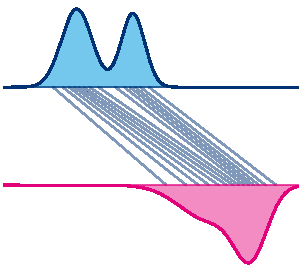
\includegraphics[height=4.6cm,width=5.1cm,keepaspectratio]{portada-I} &
      \centering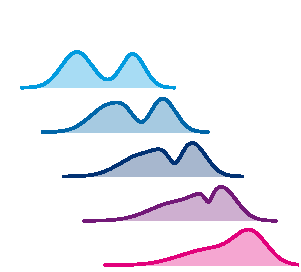
\includegraphics[height=4.6cm,width=5.1cm,keepaspectratio]{portada-II} &
      \centering\arraybackslash
\includegraphics[height=4.6cm,width=5.1cm,keepaspectratio]{portada-III}\\[6pt]
      \centering{\small\color{icnavy}\textsc{Capítulo 8}\newline Dimensión uno}\par\vspace{2pt}
        {\scriptsize\color{icnavy!70}El mapa monótono empareja los cuantiles de $\mu$ con los de $\nu$: las líneas no se cruzan} &
      \centering{\small\color{icnavy}\textsc{Capítulo 10}\newline Distancias de Wasserstein}\par\vspace{2pt}
        {\scriptsize\color{icnavy!70}La interpolación por desplazamiento: la geodésica de $W_2$ entre $\mu$ y $\nu$} &
      \centering\arraybackslash{\small\color{icnavy}\textsc{Capítulos 12--13}\newline Baricentros y Sinkhorn}\par\vspace{2pt}
        {\scriptsize\color{icnavy!70}Baricentro entrópico de un disco, un cuadrado y un triángulo}
    \end{tabular}};
  % logos
  \node[anchor=south] at ([xshift=-1.45cm,yshift=2.25cm]current page.south) {
\includegraphics[height=1.9cm]{IC.jpeg}};
  \node[anchor=south] at ([xshift=2.95cm,yshift=2.25cm]current page.south) {
\includegraphics[height=1.9cm]{DM.png}};
  \node[anchor=south,align=center,font=\small,text=icnavy!75] at ([xshift=0.75cm,yshift=1.15cm]current page.south)
    {Instituto de Cálculo, FCEN--CONICET \quad$\cdot$\quad Departamento de Matemática, FCEN--UBA};
\end{tikzpicture}
\null
\clearpage

%% REVERSO DE LA PORTADA
\thispagestyle{empty}
\null\vfill
\begin{flushleft}\small
Julián Fernández Bonder\\
Instituto de Cálculo, FCEN--CONICET\\
Departamento de Matemática, FCEN--UBA\\
Ciudad Universitaria, Pabellón 0+$\infty$ (1428), Buenos Aires, Argentina.\\[6pt]
{\it Correo:} \href{mailto:jfbonder@dm.uba.ar}{\texttt{jfbonder@dm.uba.ar}}\\
{\it URL:} \url{https://mate.dm.uba.ar/~jfbonder/}\\[12pt]
Notas del curso \emph{Teoría de Transporte Óptimo}, optativa para las Licenciaturas en
Matemática y en Ciencia de Datos y para el Doctorado en Matemática,
FCEN--UBA, 2do cuatrimestre de 2026.\\[12pt]
Sitio de la materia, con las guías de ejercicios y los cuadernos de cómputo:\\
\url{https://jfbonder.github.io/transporte-optimo/}\\[12pt]
Texto y figuras: licencia CC BY-NC-SA 4.0. Código: licencia MIT.
\end{flushleft}
\clearpage

\cleardoublepage
\chapter*{Prefacio}
{\renewcommand{\thefigure}{P.\arabic{figure}}%

Estas notas fueron escritas durante el dictado de la materia \emph{Teoría de
Transporte Óptimo}, curso optativo para las Licenciaturas en Matemática y en
Ciencia de Datos y para el Doctorado en Matemática de la Facultad de Ciencias
Exactas y Naturales de la Universidad de Buenos Aires, en el segundo
cuatrimestre de 2026. Nacieron como apuntes de clase que se fueron publicando
capítulo a capítulo a medida que avanzaba el curso, y conservan ese carácter:
son notas de un curso de un cuatrimestre, no un tratado, y su versión actual
es todavía preliminar. Las correcciones y sugerencias son bienvenidas.

\subsection*{De qué trata el tema}

El problema del transporte óptimo tiene un origen concreto. Supongamos que se
tiene un depósito de tierra y un pozo que se quiere llenar con ella; mover la
tierra cuesta un esfuerzo que depende de dónde se la toma y de dónde se la
deposita. ¿Cómo realizar el transporte a costo mínimo?
Modelando el depósito y el pozo como medidas de probabilidad $\mu$ y $\nu$, y
el esfuerzo como una función de costo $c(x,y)$ (Figura~\ref{fig.prefacio.monge}),
la pregunta se convierte en un problema variacional que Gaspard Monge planteó
en 1781 y que Leonid Kantorovich reformuló en la década de 1940, dando lugar a
la dualidad que hoy lleva su nombre. A partir del trabajo de Yann Brenier
sobre la factorización polar, anunciado en 1987~\cite{Brenier1987} y
publicado en detalle en 1991~\cite{Brenier1991}, la teoría experimentó un desarrollo extraordinario y se convirtió en un
punto de encuentro entre el análisis, la geometría, la probabilidad, las
ecuaciones en derivadas parciales y la optimización.

\begin{figure}[htbp]
\centering
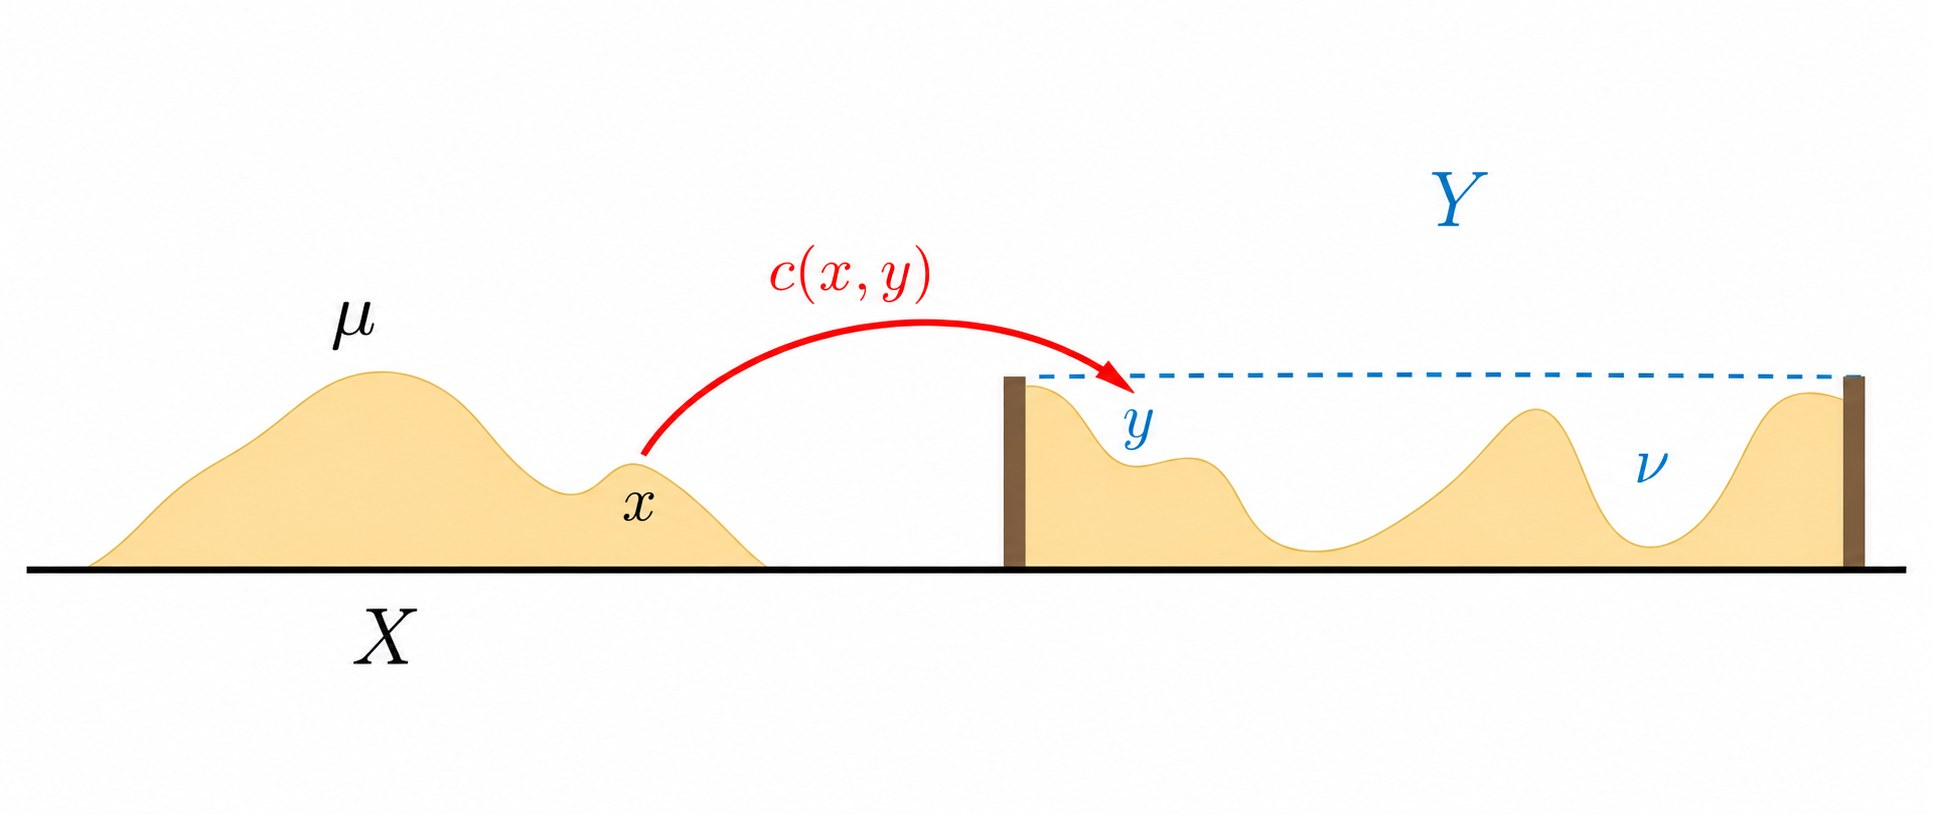
\includegraphics[width=0.75\textwidth]{fig-monge-arena.jpg}
\caption{El problema original de Monge: transportar una distribución de masa
$\mu$ sobre $X$ hacia otra distribución $\nu$ sobre $Y$, minimizando el costo
total de transporte.}
\label{fig.prefacio.monge}
\end{figure}

\begin{figure}[htbp]
\centering
\begin{minipage}[t]{0.3\textwidth}\centering
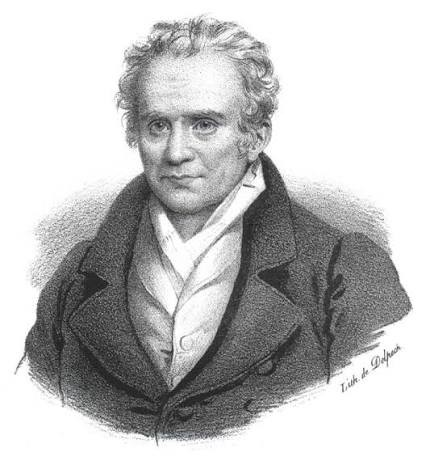
\includegraphics[height=3.6cm]{retrato-monge.jpg}\\[3pt]
{\small Gaspard Monge (1746--1818)\\ El problema del transporte (1781)}
\end{minipage}\hfill
\begin{minipage}[t]{0.3\textwidth}\centering
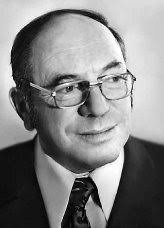
\includegraphics[height=3.6cm]{retrato-kantorovich.jpg}\\[3pt]
{\small Leonid Kantorovich (1912--1986)\\ Premio Nobel de Economía (1975)}
\end{minipage}\hfill
\begin{minipage}[t]{0.3\textwidth}\centering
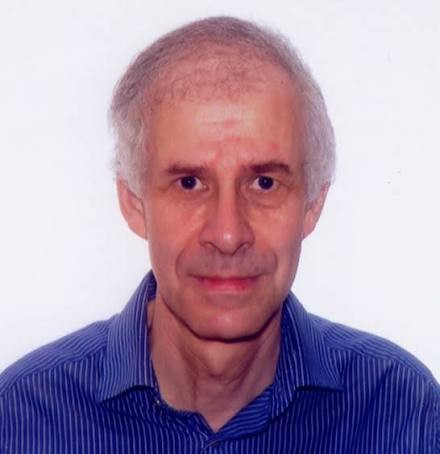
\includegraphics[height=3.6cm]{retrato-brenier.jpg}\\[3pt]
{\small Yann Brenier (1957--)\\ Teorema de factorización polar (1987)}
\end{minipage}
\caption{Tres nombres en la historia del transporte óptimo.}
\label{fig.prefacio.retratos}
\end{figure}

En las últimas dos décadas, además, el transporte óptimo pasó a ocupar un
lugar central en estadística, ciencia de datos y aprendizaje automático: la
distancia de Wasserstein se convirtió en una herramienta fundamental para
comparar distribuciones de probabilidad y aparece en problemas de inferencia
estadística, procesamiento de imágenes, visión por computadora, aprendizaje
profundo y modelos generativos (Figura~\ref{fig.prefacio.aplicaciones}).

\begin{figure}[htbp]
\centering
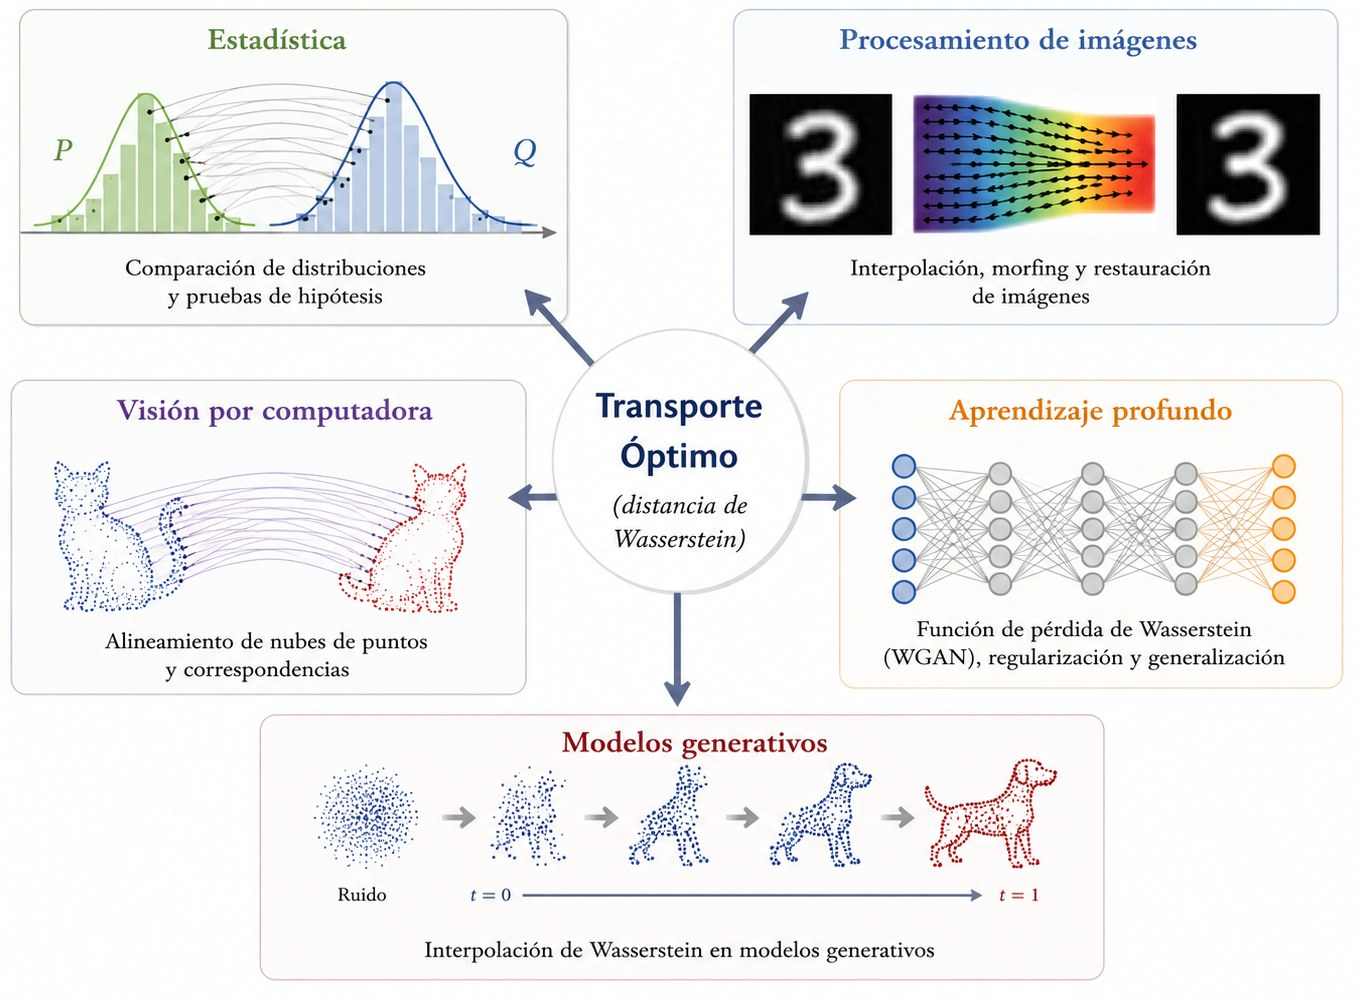
\includegraphics[width=0.9\textwidth]{fig-aplicaciones.jpg}
\caption{Algunas aplicaciones contemporáneas del transporte óptimo y de la
distancia de Wasserstein.}
\label{fig.prefacio.aplicaciones}
\end{figure}

\subsection*{Contenido y organización}

El objetivo del curso es presentar los fundamentos matemáticos de la teoría
moderna del transporte óptimo, con énfasis en sus aspectos analíticos y
geométricos, y una mirada a los aspectos computacionales. La primera parte
(Capítulos~\ref{cap.intro} a~\ref{cap.Brenier}) recorre el problema de Monge
y la relajación de Kantorovich, la existencia de planes óptimos, la dualidad
y los potenciales de Kantorovich, el caso unidimensional y el teorema de
factorización polar de Brenier. La segunda parte (Capítulos~\ref{cap.Wp}
a~\ref{cap.Sinkhorn}) estudia las distancias de Wasserstein y la geometría
del espacio de medidas de probabilidad, con una aplicación a la desigualdad
de Brunn--Minkowski, los baricentros de Wasserstein y la regularización
entrópica con el algoritmo de Sinkhorn. Cinco apéndices reúnen el material
auxiliar: complementos de teoría de la medida, el teorema de
Fenchel--Rockafellar, la factorización polar de matrices, el subdiferencial
de funciones convexas y una guía de los cuadernos de cómputo.

Se asume familiaridad con el análisis real y con los rudimentos de la teoría
de la medida, que se repasan en el Apéndice~\ref{ap.medida}. Cada capítulo
termina con una sección de ejercicios; en seis de ellos hay además ejercicios
computacionales, que se resuelven con cuadernos de Python que acompañan las
notas. El curso siguió principalmente los textos de Villani~\cite{Villani2003}
y Santambrogio~\cite{Santambrogio}; para los aspectos computacionales, el de
Peyré y Cuturi~\cite{PeyreCuturi2019}. Los ejercicios marcados con
($\bigstar$) son de mayor dificultad o exceden el programa del curso; pueden
omitirse en una primera lectura.

\subsection*{Convenciones}

Salvo indicación en contrario, los espacios $X$, $Y$ son \emph{espacios
polacos}, es decir, espacios métricos completos y separables (por ejemplo,
$\R^d$ o un subconjunto cerrado de $\R^d$), y todas las medidas son
borelianas. Un \emph{acoplamiento} de dos variables aleatorias, o de dos
medidas $\mu$ y $\nu$, es una medida en el producto con marginales $\mu$ y
$\nu$; en el lenguaje de estas notas, un plan de transporte
(Sección~\ref{sec.interp.prob}). Para dos medidas finitas $\mu$, $\nu$,
$\mu\wedge\nu$ denota la mayor medida que está por debajo de ambas
(si $\mu=f\lambda$ y $\nu=g\lambda$, es $\min\{f,g\}\lambda$), y
$(\mu-\nu)^\pm$ son las partes positiva y negativa de la medida signada
$\mu-\nu$; así, $\mu=\mu\wedge\nu+(\mu-\nu)^+$. Para $p\ge1$,
$\mathcal P_p(\R^d)$ es el conjunto de medidas de probabilidad con momento de
orden $p$ finito, $\int|x|^p\,d\mu<\infty$ (Definición~\ref{def.Pp}); lo
usamos en algunos ejercicios anteriores al Capítulo~\ref{cap.Brenier}, donde
se lo introduce formalmente.

\subsection*{El material del curso}

Todo el material está sistematizado en el sitio del curso,
\begin{center}
\url{https://jfbonder.github.io/transporte-optimo/}
\end{center}
donde se encuentran estas notas, las guías de ejercicios de cada capítulo
(que son exactamente las secciones de ejercicios de las notas, con la misma
numeración), un archivo de sugerencias para los ejercicios y los seis
cuadernos de Python, que pueden abrirse directamente en Google Colab. El
sitio y las fuentes de todo el material están en un repositorio público,
donde también pueden reportarse erratas.

\subsection*{Sobre la redacción}

En la confección de estas notas se utilizaron herramientas de inteligencia
artificial. La selección de los temas, el orden de la exposición, las
decisiones sobre qué demostrar y qué remitir a la bibliografía, y la revisión
final de cada capítulo son del autor; una parte sustancial de la redacción,
de las demostraciones detalladas, de los ejercicios y de los cuadernos de
cómputo fue producida en diálogo con asistentes de IA, a partir de
indicaciones del autor y sujeta a su revisión. Este modo de trabajo hizo
posible escribir, en un cuatrimestre, un material más completo del que
hubiera sido posible de otro modo; también obliga a una advertencia: la
responsabilidad por los errores que hayan quedado es exclusivamente del
autor, y agradeceré que me los señalen.
%% La firma cerraba el prefacio sola al principio de una página. La bajamos al
%% final de la anterior: \nobreak impide el corte en el salto vertical, y
%% \enlargethispage le da a esa página el espacio que falta.
\enlargethispage{3.2\baselineskip}
\par\nobreak
\medskip
\nobreak
\noindent Buenos Aires, septiembre de 2026.
\hfill Julián Fernández Bonder
}
\cleardoublepage
\tableofcontents 


%%%%%%%%%%%%%%%%%%%%%%%%%%%%%%%%%%%%%%%%
%% INTRODUCCION %%%%%%%%%%%%%%%%%%%%%%%%%%%%%
%%%%%%%%%%%%%%%%%%%%%%%%%%%%%%%%%%%%%%%%
\chapter{Introducción}\label{cap.intro}


El problema del transporte óptimo admite dos formulaciones clásicas, y la
paso de una a otra organiza buena parte de la teoría, que gira en torno a la
pregunta de cuándo la segunda recupera a la primera. La primera es la de
Monge: llevar una distribución de masa sobre otra mediante una aplicación que
asigna a cada punto de origen un único destino, de modo que el costo total del
traslado sea mínimo. La segunda es la de Kantorovich: en lugar de una
aplicación, un plan de transporte, que permite repartir la masa que hay en un
punto entre varios destinos. Este capítulo introduce ambas y explica por qué la
segunda es la formulación que admite un tratamiento riguroso.

La Sección~\ref{sec.monge} presenta el problema de Monge tal como él lo planteó
en 1781, primero en el caso discreto de depósitos y pozos con cantidades
finitas de material y después en el caso continuo, con densidades, y discute
qué funciones de costo son razonables y cuáles son las que aparecen en la
práctica.

La Sección~\ref{sec.monge.medidas} traduce las dos versiones a un lenguaje
común, el de las medidas de probabilidad, en el que la condición de que la
aplicación $T$ transporte la masa de $\mu$ sobre la de $\nu$ se escribe
$T_\#\mu=\nu$ mediante la medida imagen. Esa traducción deja a la vista las dos
dificultades del problema de Monge. Por un lado, puede no haber ninguna
aplicación admisible: si $\mu$ es una delta y $\nu$ tiene dos átomos, no hay
manera de partir la masa. Por otro, aun cuando las haya, la restricción
$T_\#\mu=\nu$ es no lineal en $T$ y el conjunto de aplicaciones admisibles no es
convexo, de modo que el método directo del cálculo de variaciones no se puede
aplicar: una sucesión minimizante no tiene por qué converger a una aplicación
admisible.

La Sección~\ref{sec.kantorovich} introduce la relajación que propuso
Kantorovich en la década de 1940. Un plan de transporte es una medida $\pi$
sobre el producto $X\times Y$ cuyas marginales son $\mu$ y $\nu$; el conjunto
$\Pi(\mu,\nu)$ de todos ellos nunca es vacío, porque contiene a
$\mu\otimes\nu$, es convexo, y el costo es lineal en $\pi$. Cada aplicación
admisible induce un plan concentrado en su gráfico, así que el problema de
Kantorovich es efectivamente una relajación del de Monge. El precio a pagar es
que el mínimo de Kantorovich no siempre proviene de una aplicación; decidir
cuándo sí lo hace es el contenido del teorema de Brenier
(Capítulo~\ref{cap.Brenier}).

La Sección~\ref{sec.interp.prob} reinterpreta los planes en términos
probabilísticos, como acoplamientos de variables aleatorias con distribuciones
dadas, que es el punto de vista natural cuando el transporte óptimo se usa en
estadística.

La Sección~\ref{sec.intro.discreto} vuelve al caso discreto, donde el problema
de Kantorovich es un problema de programación lineal en dimensión finita. El
teorema de Birkhoff--von Neumann identifica los puntos extremales del conjunto
de matrices biestocásticas con las permutaciones y permite deducir que, cuando
las dos medidas son sumas de la misma cantidad de deltas con pesos iguales, el
problema de Monge sí tiene solución. Este caso se retoma en los
Capítulos~\ref{cap.PL} y~\ref{cap.dual.discreto}.

\section{El problema de Monge}\label{sec.monge}

En 1781, Gaspard Monge estudió el problema de los desmontes y terraplenes: dada una región de la que debe extraerse cierta cantidad de tierra y otra que debe rellenarse con el mismo volumen, ¿cómo organizar el transporte minimizando el costo total?

\subsection{El caso discreto}

Supongamos que tenemos \(n\) depósitos de tierra, ubicados en los puntos
\[
x_1,\dots,x_n,
\]
y \(m\) pozos, ubicados en
\[
y_1,\dots,y_m.
\]
El depósito \(x_i\) contiene una cantidad \(a_i>0\) de tierra y el pozo \(y_j\) tiene capacidad \(b_j>0\), donde
\[
\sum_{i=1}^n a_i=\sum_{j=1}^m b_j.
\]

Transportar una unidad de tierra desde \(x_i\) hasta \(y_j\) tiene un costo
\[
c(x_i,y_j).
\]

Si cada depósito debe enviarse íntegramente a un único pozo, una estrategia de transporte está dada por una aplicación
\[
T\colon \{x_1,\dots,x_n\}\longrightarrow \{y_1,\dots,y_m\}.
\]

No toda aplicación es admisible. Para cada pozo \(y_j\), la cantidad total de tierra que recibe debe coincidir con su capacidad, es decir,
\[
\sum_{T(x_i)=y_j} a_i=b_j,
\qquad j=1,\dots,m.
\]

El costo total asociado a la aplicación \(T\) es
\[
C(T)=\sum_{i=1}^n c(x_i,T(x_i))\,a_i.
\]

El problema de Monge consiste en encontrar, entre todas las aplicaciones admisibles, aquella que minimiza el costo total de transporte.

\subsection{El caso continuo}

Supongamos ahora que la tierra ocupa una región \(X\subset\mathbb{R}^d\) con densidad \(\rho_0\), mientras que la excavación ocupa una región \(Y\subset\mathbb{R}^d\) con densidad objetivo \(\rho_1\). Supondremos que ambas contienen la misma cantidad total de masa,
\[
\int_X \rho_0(x)\,dx
=
\int_Y \rho_1(y)\,dy.
\]

Una estrategia de transporte consiste en una aplicación
\[
T\colon X\longrightarrow Y,
\]
que indica a qué punto de la excavación se traslada cada partícula de tierra.

Si transportar una unidad de masa desde \(x\) hasta \(T(x)\) tiene un costo
\[
c(x,T(x)),
\]
el costo total del transporte viene dado por
\[
C(T)=\int_X c(x,T(x))\,\rho_0(x)\,dx.
\]

La aplicación \(T\) debe preservar la masa. Es decir, para toda región medible \(B\subset Y\), la cantidad de tierra que llega a \(B\) debe coincidir con la capacidad de dicha región:
\[
\int_{T^{-1}(B)} \rho_0(x)\,dx
=
\int_B \rho_1(y)\,dy.
\]

El problema de Monge consiste entonces en minimizar el costo total entre todas las aplicaciones que satisfacen esta condición de preservación de la masa.

\subsection{Funciones de costo}
La función
\[
c:X\times Y\to[0,\infty]
\]
representa el costo de transportar una unidad de masa desde \(x\) hasta \(y\).

Entre los costos más utilizados se encuentran:

\begin{enumerate}
\item El costo lineal
\[
c(x,y)=|x-y|,
\]
que modela un costo proporcional a la distancia recorrida.

\item El costo cuadrático
\[
c(x,y)=|x-y|^2,
\]
que es el más estudiado en la teoría moderna del transporte óptimo.

\item Más generalmente,
\[
c(x,y)=|x-y|^p,
\qquad p\ge1,
\]
que conduce a las distancias de Wasserstein \(W_p\), que estudiaremos más adelante.
\end{enumerate}


\section{El problema de Monge en espacios de medida}\label{sec.monge.medidas}

La formulación de la sección anterior distingue entre el caso discreto y el
continuo. Ambos pueden tratarse dentro de un mismo marco utilizando la noción
de medida, que además permite considerar espacios mucho más generales que
$\mathbb R^d$. Las nociones de teoría de la medida que necesitamos
---$\sigma$-álgebras, medidas de probabilidad, funciones medibles, integral,
y los ejemplos básicos de medidas de Dirac, discretas y con densidad--- se
recuerdan en el Apéndice~\ref{ap.medida}, Sección~\ref{sec.ap.medida.repaso},
junto con la notación que usaremos: $\mathcal P(X)$ para las medidas de
probabilidad sobre $X$, $\mathcal B(X)$ para los borelianos de un espacio
métrico y $\mathcal L^d$ para la medida de Lebesgue en $\mathbb R^d$.


Hasta ahora hemos estudiado dos versiones del problema de transporte: una discreta, en la que la masa está concentrada en un número finito de puntos, y otra continua, en la que la distribución de masa está descripta mediante funciones de densidad. En esta sección veremos que ambas formulaciones pueden expresarse de una manera unificada utilizando medidas.

\subsection{El caso discreto}

Recordemos que el problema discreto consiste en transportar masas \(a_1,\dots,a_n\) ubicadas en los puntos \(x_1,\dots,x_n\) hacia masas \(b_1,\dots,b_m\) ubicadas en los puntos \(y_1,\dots,y_m\), satisfaciendo
\[
\sum_{i=1}^n a_i=\sum_{j=1}^m b_j.
\]

Estas distribuciones de masa pueden representarse mediante las medidas discretas
\[
\mu=\sum_{i=1}^n a_i\,\delta_{x_i},
\qquad
\nu=\sum_{j=1}^m b_j\,\delta_{y_j}.
\]

Si \(T\colon\{x_1,\dots,x_n\}\to\{y_1,\dots,y_m\}\) es una aplicación que transporta la masa inicial a la final, la condición de conservación de la masa puede escribirse como
\[
\nu(B)=\mu(T^{-1}(B))
\]
para todo subconjunto \(B\subset\{y_1,\dots,y_m\}\).

Por otra parte, el costo total del transporte puede escribirse como
\[
\sum_{i=1}^n c(x_i,T(x_i))\,a_i
=
\int c(x,T(x))\,d\mu(x).
\]

\subsection{El caso continuo}

Supongamos ahora que \(X=Y=\mathbb R^d\) y que las distribuciones inicial y final poseen densidades \(\rho_0\) y \(\rho_1\), respectivamente. Es decir,
\[
d\mu(x)=\rho_0(x)\,dx,
\qquad
d\nu(y)=\rho_1(y)\,dy.
\]

Recordemos que la condición de conservación de la masa puede expresarse como
\[
\int_{T^{-1}(B)} \rho_0(x)\,dx
=
\int_B \rho_1(y)\,dy
\]
para todo conjunto boreliano \(B\subset\mathbb R^d\).

Utilizando las medidas \(\mu\) y \(\nu\), esta condición puede reescribirse simplemente como
\[
\nu(B)=\mu(T^{-1}(B)).
\]

Asimismo, el costo del transporte
\[
\int_{\mathbb R^d} c(x,T(x))\,\rho_0(x)\,dx
\]
puede escribirse como
\[
\int_{\mathbb R^d} c(x,T(x))\,d\mu(x).
\]
Esto motiva la siguiente formulación general del problema de Monge.

\begin{defi}[Problema de Monge]
Sean \(X\) e \(Y\) espacios medibles, \(\mu\in\mathcal P(X)\) y
\(\nu\in\mathcal P(Y)\), y sea
\[
c\colon X\times Y\to[0,\infty]
\]
una función de costo.

El \emph{problema de Monge} consiste en encontrar una aplicación medible
\[
T\colon X\to Y
\]
que minimice el costo total de transporte
\[
\int_X c(x,T(x))\,d\mu(x),
\]
entre todas las aplicaciones $T$ que satisfacen la condición de conservación de la masa
\[
\nu(B)=\mu(T^{-1}(B))
\]
para todo conjunto medible \(B\subset Y\).

Equivalentemente,
\[
\min\left\{
\int_X c(x,T(x))\,d\mu(x)
:
\begin{array}{l}
T\colon X\to Y,\\[1mm]
\nu(B)=\mu(T^{-1}(B))
\quad\forall\,B\in\mathcal B(Y)
\end{array}
\right\}.
\]
\end{defi}

La condición de conservación de la masa
\[
\nu(B)=\mu(T^{-1}(B)),
\qquad
B\in\mathcal B(Y),
\]
aparece de manera recurrente en la teoría del transporte óptimo. Esto motiva introducir una notación específica para la medida obtenida al transportar una medida mediante una aplicación.
\begin{defi}[Medida imagen]
Sean \((X,\mathcal A)\) e \((Y,\mathcal B)\) espacios medibles,
\(\mu\in\mathcal M_+(X)\) y
\(T\colon X\to Y\) una aplicación medible.

La \emph{medida imagen} (o \emph{push-forward}) de \(\mu\) mediante \(T\) es la medida \(T_\#\mu\in\mathcal M_+(Y)\) definida por
\[
T_\#\mu(B)=\mu(T^{-1}(B))
\]
para todo \(B\in\mathcal B\).
\end{defi}

Con esta notación el Problema de Monge queda formulado como:
\begin{equation}\tag{PM}\label{PM}
\min\left\{
\int_X c(x,T(x))\,d\mu(x)
:
\begin{array}{l}
T\colon X\to Y\ \text{medible},\\
T_\#\mu=\nu.
\end{array}
\right\}.
\end{equation}

En general, la función
\[
c\colon X\times Y\to[0,\infty]
\]
representa el costo de transportar una unidad de masa desde \(x\in X\) hasta \(y\in Y\). La teoría que desarrollaremos es válida para funciones de costo bastante generales.

En muchos de los problemas que estudiaremos, el espacio de partida y de llegada coinciden y están provistos de una distancia \(d\). En ese caso, una familia natural de funciones de costo está dada por
\[
c(x,y)=d(x,y)^p,
\qquad p\ge1,
\]
que generaliza los costos $c(x,y)=|x-y|^p$ considerados en $\R^d$.

\section{La relajación de Kantorovich}\label{sec.kantorovich}

El problema de Monge \eqref{PM} presenta tres dificultades analíticas importantes.

En primer lugar, la condición de conservación de la masa impuesta sobre la aplicación \(T\) es muy restrictiva, por lo que el conjunto de aplicaciones admisibles puede ser vacío. En consecuencia, el problema puede no tener solución.

\begin{ejem}
Sea
\[
\mu=\delta_{x_0},
\]
y supongamos que \(\nu\) no es una medida de Dirac.

No existe ninguna aplicación \(T\colon X\to Y\) tal que
\[
T_\#\mu=\nu.
\]

En efecto, si existiera, la imagen de toda la masa concentrada en \(x_0\) debería enviarse a un único punto \(T(x_0)\), por lo que
\[
T_\#\mu=\delta_{T(x_0)},
\]
que sigue siendo una medida de Dirac.
\end{ejem}

Por otra parte, aun cuando exista una aplicación admisible, la restricción
\[
T_\#\mu=\nu
\]
es altamente no lineal. En el caso en que
\[
d\mu=\rho_0(x)\,dx,
\qquad
d\nu=\rho_1(y)\,dy,
\]
y \(T\) es suficientemente regular, dicha condición implica la ecuación
\[
\rho_1(T(x))\,|\det DT(x)|
=
\rho_0(x),
\]
que ya es una ecuación no lineal para \(T\). Precisamos esta afirmación
en la siguiente proposición.
\begin{prop}\label{prop.cambio.variables}
Sea $\Omega\subset\R^d$ abierto. Supongamos que $\mu=\rho_0\,dx$,
$\nu=\rho_1\,dx$ son medidas en $\Omega$ y que
$T:\Omega\to\Omega$ es un difeomorfismo de clase $C^1$ que satisface
$T_{\#}\mu=\nu$.

Entonces
\[
\rho_1(T(x))\,|\det DT(x)|
=
\rho_0(x)
\]
para casi todo $x\in\Omega$ (y para todo $x$ si $\rho_0$ y $\rho_1$ son continuas).
\end{prop}

\begin{proof}
Como $T_{\#}\mu=\nu$, para todo boreliano $B\subset\Omega$ se tiene
\[
\mu(T^{-1}(B))
=
\nu(B),
\]
es decir,
\[
\int_{T^{-1}(B)}
\rho_0(x)\,dx
=
\int_B
\rho_1(y)\,dy.
\]

Aplicando el teorema de cambio de variables con
$y=T(x)$ obtenemos
\[
\int_{T^{-1}(B)}
\rho_0(x)\,dx
=
\int_B
\rho_0(T^{-1}(y))
\,
\left|
\det DT^{-1}(y)
\right|
\,dy.
\]

Comparando con la identidad anterior, concluimos que
\[
\rho_1(y)
=
\rho_0(T^{-1}(y))
\,
\left|
\det DT^{-1}(y)
\right|
\]
para casi todo $y\in\Omega$.

Finalmente, sustituyendo $y=T(x)$ y usando la identidad
\[
DT^{-1}(T(x))
=
(DT(x))^{-1},
\]
obtenemos
\[
\left|
\det DT^{-1}(T(x))
\right|
=
\frac{1}{|\det DT(x)|},
\]
de donde
\[
\rho_1(T(x))
=
\frac{\rho_0(x)}
{|\det DT(x)|},
\]
o, equivalentemente,
\[
\rho_1(T(x))
\,|\det DT(x)|
=
\rho_0(x),
\]
como queríamos demostrar.
\end{proof}

\begin{obs}
La identidad
\[
\rho_1(T(x))\,|\det DT(x)|=\rho_0(x)
\]
es una consecuencia del teorema de cambio de variables y corresponde al caso en
que el dominio y el codominio tienen la misma dimensión.

Cuando $X=\mathbb{R}^d$ e $Y=\mathbb{R}^k$ con $k\neq d$, se obtienen relaciones
análogas entre las densidades mediante las fórmulas de área y de coárea, que
constituyen extensiones naturales del teorema de cambio de variables. Para una
presentación detallada de estos resultados remitimos al libro de
Evans y Gariepy~\cite{EvansGariepy}.
\end{obs}

Volvamos a la lista de dificultades del problema de Monge. La tercera es que, incluso cuando el conjunto de aplicaciones admisibles no es vacío, presenta serias dificultades analíticas: en general no es cerrado para topologías razonables sobre las aplicaciones, de modo que extraer límites de sucesiones minimizantes no es inmediato. Estas obstrucciones hacen que el método directo del cálculo de variaciones no sea directamente aplicable al problema de Monge.

Estas dificultades motivaron a Leonid Kantorovich a proponer una relajación del problema de Monge. La idea fundamental consiste en abandonar la búsqueda de una aplicación de transporte. En lugar de imponer que toda la masa situada en un punto \(x\in X\) deba enviarse a un único punto de destino, se permite dividir esa masa entre distintos puntos de llegada.

Para describir esta situación, en lugar de una aplicación se considera una medida de probabilidad
\[
\pi\in\mathcal P(X\times Y),
\]
llamada \emph{plan de transporte}. Intuitivamente,
\(
\pi(A\times B)
\)
representa la cantidad de masa que se transporta desde el conjunto \(A\subset X\) hasta el conjunto \(B\subset Y\).

En consecuencia,
\(
\pi(A\times Y)
\)
representa la masa total que sale de \(A\), mientras que
\(
\pi(X\times B)
\)
representa la masa total que llega a \(B\). La conservación de la masa exige entonces que
\[
\pi(A\times Y)=\mu(A),
\qquad
A\in\mathcal B(X),
\]
y
\[
\pi(X\times B)=\nu(B),
\qquad
B\in\mathcal B(Y).
\]

Si denotamos por
\[
\pp_1(x,y)=x,
\qquad
\pp_2(x,y)=y,
\]
las proyecciones canónicas sobre la primera y segunda componente, las condiciones anteriores pueden escribirse de forma más compacta como
\[
(\pp_1)_\#\pi=\mu,
\qquad
(\pp_2)_\#\pi=\nu.
\]

Esto motiva la siguiente definición.

\begin{defi}[Plan de transporte]
Sean \(\mu\in\mathcal P(X)\) y \(\nu\in\mathcal P(Y)\). Un \emph{plan de transporte} entre \(\mu\) y \(\nu\) es una medida
\[
\pi\in\mathcal P(X\times Y)
\]
cuyas marginales son \(\mu\) y \(\nu\), es decir,
\[
(\pp_1)_\#\pi=\mu,
\qquad
(\pp_2)_\#\pi=\nu.
\]

Denotaremos por
\[
\Pi(\mu,\nu)
\]
al conjunto de todos los planes de transporte entre \(\mu\) y \(\nu\).
\end{defi}

El costo asociado a un plan de transporte \(\pi\in\Pi(\mu,\nu)\) se define por
\[
\int_{X\times Y} c(x,y)\,d\pi(x,y),
\]
que representa el costo total de transportar la masa de acuerdo con el plan \(\pi\).

De esta manera, la relajación de Kantorovich del problema de Monge consiste en resolver
\begin{equation}\tag{PK}\label{PK}
\min\left\{
\int_{X\times Y} c(x,y)\,d\pi(x,y)
:
\pi\in\Pi(\mu,\nu)
\right\}.
\end{equation}

El problema de Kantorovich es efectivamente una relajación del problema de Monge. En efecto, dada una aplicación de transporte
\[
T\colon X\to Y,
\]
es posible asociarle el plan de transporte
\[
\pi_T=(\id,T)_\#\mu,
\]
donde
\[
(\id,T)\colon X\to X\times Y,
\qquad
x\mapsto (x,T(x)).
\]

Es inmediato verificar que
\[
\pi_T\in\Pi(\mu,\nu)
\]
si y solo si
\[
T_\#\mu=\nu,
\]
y además
\[
\int_{X\times Y}c(x,y)\,d\pi_T(x,y)
=
\int_X c(x,T(x))\,d\mu(x).
\]

Por lo tanto, toda aplicación admisible para el problema de Monge induce un plan admisible para el problema de Kantorovich con el mismo costo.

El problema de Kantorovich \eqref{PK} presenta ventajas importantes respecto del problema de Monge \eqref{PM}.

En primer lugar, el conjunto de planes admisibles nunca es vacío. En efecto, siempre contiene a la medida producto
\[
\mu\otimes\nu,
\]
ya que
\[
(\pp_1)_\#(\mu\otimes\nu)=\mu,
\qquad
(\pp_2)_\#(\mu\otimes\nu)=\nu.
\]

En segundo lugar, tanto la función de costo
\[
\pi\mapsto
\int_{X\times Y} c(x,y)\,d\pi(x,y)
\]
como las restricciones
\[
(\pp_1)_\#\pi=\mu,
\qquad
(\pp_2)_\#\pi=\nu,
\]
son lineales con respecto al plan de transporte \(\pi\). Por lo tanto, el problema de Kantorovich puede interpretarse como un problema de programación lineal en un espacio de dimensión infinita.

Estas dos propiedades hacen que el problema de Kantorovich sea mucho más tratable desde el punto de vista analítico y constituyen una de las principales razones de su enorme desarrollo.

Como veremos más adelante, el problema de Kantorovich admite, bajo hipótesis muy generales sobre el costo y las medidas, al menos un plan de transporte óptimo
\[
\pi^*\in\Pi(\mu,\nu).
\]

Sin embargo, dicho plan óptimo no tiene por qué estar inducido por una aplicación de transporte. Una de las cuestiones centrales de la teoría del transporte óptimo consiste precisamente en determinar bajo qué condiciones existe una aplicación
\[
T^*\colon X\to Y
\]
tal que
\[
\pi^*=\pi_{T^*}.
\]

Cuando esto ocurre, el plan óptimo de Kantorovich proporciona automáticamente una solución del problema original de Monge. En efecto, como ambos problemas tienen el mismo costo para los planes inducidos por aplicaciones de transporte, se concluye que \(T^*\) es un transporte óptimo para el problema de Monge.

\begin{figure}[ht]
\centering
\begin{tikzpicture}[fig]
  % ---------- panel izquierdo: plan inducido por un mapa ----------
  \begin{scope}
    \draw[eje] (-0.3,0) -- (3.6,0) node[rotulo,right] {$X$};
    \draw[eje] (0,-0.3) -- (0,3.1) node[rotulo,above] {$Y$};
    % átomos de mu en el eje X
    \foreach \x/\lbl in {0.7/x_1, 1.8/x_2, 2.9/x_3} {
      \node[pt,minimum size=3pt,black] at (\x,0) {}; \node[anota,below=2pt] at (\x,0) {$\lbl$};
    }
    % átomos de nu en el eje Y
    \foreach \y/\lbl in {0.9/y_1, 2.3/y_2} {
      \node[pt,minimum size=3pt,black] at (0,\y) {}; \node[anota,left=2pt] at (0,\y) {$\lbl$};
    }
    % grilla tenue
    \foreach \x in {0.7,1.8,2.9} \draw[grilla] (\x,0) -- (\x,3);
    \foreach \y in {0.9,2.3}     \draw[grilla] (0,\y) -- (3.5,\y);
    % plan de Monge: T(x1)=y1, T(x2)=y2, T(x3)=y1
    % masas a=(1/4,3/8,3/8); radios proporcionales a sqrt(a_i)
    \node[ptmasa,figmain,minimum size=7.44pt] at (0.7,0.9) {};
    \node[ptmasa,figmain,minimum size=9.10pt] at (1.8,2.3) {};
    \node[ptmasa,figmain,minimum size=9.10pt] at (2.9,0.9) {};
    \node[rotulo,below=6pt,align=center] at (1.75,-0.55)
      {plan inducido por un mapa\\ $\pi_T=(\id,T)_\#\mu$};
  \end{scope}
  % ---------- panel derecho: plan que divide masa ----------
  \begin{scope}[xshift=\figpanelsep]
    \draw[eje] (-0.3,0) -- (3.6,0) node[rotulo,right] {$X$};
    \draw[eje] (0,-0.3) -- (0,3.1) node[rotulo,above] {$Y$};
    \foreach \x/\lbl in {0.7/x_1, 1.8/x_2, 2.9/x_3} {
      \node[pt,minimum size=3pt,black] at (\x,0) {}; \node[anota,below=2pt] at (\x,0) {$\lbl$};
    }
    \foreach \y/\lbl in {0.9/y_1, 2.3/y_2} {
      \node[pt,minimum size=3pt,black] at (0,\y) {}; \node[anota,left=2pt] at (0,\y) {$\lbl$};
    }
    \foreach \x in {0.7,1.8,2.9} \draw[grilla] (\x,0) -- (\x,3);
    \foreach \y in {0.9,2.3}     \draw[grilla] (0,\y) -- (3.5,\y);
    % plan producto: masa a_i b_j, con a=(1/4,3/8,3/8) y b=(5/8,3/8)
    % (las mismas marginales que el panel izquierdo); radios ~ sqrt(masa)
    \node[ptmasa,minimum size=5.88pt] at (0.7,0.9) {};
    \node[ptmasa,minimum size=4.56pt] at (0.7,2.3) {};
    \node[ptmasa,minimum size=7.20pt] at (1.8,0.9) {};
    \node[ptmasa,minimum size=5.58pt] at (1.8,2.3) {};
    \node[ptmasa,minimum size=7.20pt] at (2.9,0.9) {};
    \node[ptmasa,minimum size=5.58pt] at (2.9,2.3) {};
    \node[rotulo,below=6pt,align=center] at (1.75,-0.55)
      {plan que divide la masa\\ (por ejemplo, $\mu\otimes\nu$)};
  \end{scope}
\end{tikzpicture}
\caption{Dos planes de transporte entre las \emph{mismas} medidas
$\mu=\sum_i a_i\delta_{x_i}$ y $\nu=\sum_j b_j\delta_{y_j}$, con
$a=(\frac14,\frac38,\frac38)$ y $b=(\frac58,\frac38)$, vistos como medidas en
$X\times Y$; el área de cada punto es proporcional a la masa
$\pi(\{(x_i,y_j)\})$. A la izquierda, un
plan inducido por un mapa: cada columna tiene un único punto, toda la masa de
$x_i$ va a $T(x_i)$. A la derecha, un plan genuinamente de Kantorovich: la masa
de cada $x_i$ se reparte entre varios destinos. Las marginales se leen sumando
la masa de cada columna (debe dar $a_i$) y de cada fila (debe dar $b_j$).}
\label{fig.planes}
\end{figure}
 


\section{Una interpretación probabilística del problema de Kantorovich}\label{sec.interp.prob}

Hasta ahora, hemos presentado el problema de Monge como la búsqueda de
una función $T$ que mueve puntos de manera determinista. La relajación de
Kantorovich permite una interpretación probabilística particularmente
natural, si traducimos el lenguaje de medidas al de variables
aleatorias definidas sobre un espacio de probabilidad común
$(\Omega,\mathcal F,\mathbb P)$.

En la formulación de Kantorovich, las variables aleatorias $\mathbf X$ y
$\mathbf Y$ no están fijadas conjuntamente. Lo que conocemos son
únicamente sus leyes marginales
\[
\mathbf X_\#\mathbb P=\mu,
\qquad
\mathbf Y_\#\mathbb P=\nu.
\]
Estas leyes no determinan, en general, la ley conjunta de
$(\mathbf X,\mathbf Y)$. Existen, por lo tanto, muchas maneras posibles
de establecer una dependencia entre ambas variables que sean
compatibles con las mismas leyes marginales. Cada una de ellas
determina un acoplamiento
\[
\pi=(\mathbf X,\mathbf Y)_\#\mathbb P\in\Pi(\mu,\nu).
\]

Así, podemos interpretar un plan de transporte como una elección de la
estructura de dependencia entre dos variables aleatorias cuyas leyes
marginales están fijadas. Para un acoplamiento particular
$\pi\in\Pi(\mu,\nu)$, el costo de transporte es el costo esperado
\[
\mathbb E_{\pi}[c(\mathbf X,\mathbf Y)].
\]
En efecto, si $(\mathbf X,\mathbf Y)$ tiene ley conjunta $\pi$, entonces
\[
(\mathbf X,\mathbf Y)_\#\mathbb P=\pi
\]
y, por el teorema de cambio de variables,
\[
\mathbb E_{\pi}[c(\mathbf X,\mathbf Y)]
=
\int_\Omega
c(\mathbf X(\omega),\mathbf Y(\omega))\,d\mathbb P(\omega)
=
\int_{X\times Y}c(x,y)\,d\pi(x,y).
\]

El problema de Kantorovich consiste, entonces, en elegir, entre todas
las posibles leyes conjuntas con marginales $\mu$ y $\nu$, aquella que
minimiza el costo esperado:
\[
\min_{\pi\in\Pi(\mu,\nu)}
\mathbb E_{\pi}[c(\mathbf X,\mathbf Y)].
\]

Esta libertad en la elección de la ley conjunta permite que, para un
origen $x$, la masa pueda distribuirse entre varios destinos $y$. Este
fenómeno, conocido como \emph{división de masa} o \emph{mass splitting},
no es posible en general en el problema de Monge, donde cada origen
$x$ tiene asociado un único destino $T(x)$.
%
%Hasta ahora, hemos presentado el problema de Monge como la búsqueda de una función $T$ que mueve puntos de manera determinista. La relajación de Kantorovich permite una interpretación más rica si traducimos el lenguaje de medidas al de \textbf{variables aleatorias} definidas sobre un espacio de probabilidad común $(\Omega, \mathcal{F}, \mathbb{P})$.
%
%En la formulación de Kantorovich, las variables aleatorias
%$\mathbf{X}$ y $\mathbf{Y}$ no están fijadas conjuntamente. Lo que
%conocemos son únicamente sus leyes marginales
%\[
%\mathbf{X}_\#\mathbb{P}=\mu,
%\qquad
%\mathbf{Y}_\#\mathbb{P}=\nu.
%\]
%Estas leyes no determinan, en general, la ley conjunta de
%$(\mathbf{X},\mathbf{Y})$. Existen muchas maneras posibles de establecer
%una dependencia entre ambas variables que sean compatibles con las
%mismas leyes marginales. Cada una de ellas determina un acoplamiento
%\[
%\pi=(\mathbf{X},\mathbf{Y})_\#\mathbb{P}\in\Pi(\mu,\nu).
%\]
%
%Desde esta perspectiva, el problema de Kantorovich puede interpretarse
%como la búsqueda, entre todas las posibles leyes conjuntas con
%marginales $\mu$ y $\nu$, de aquella que minimiza el costo esperado:
%\[
%\min_{\pi\in\Pi(\mu,\nu)}
%\mathbb{E}_{\pi}[c(\mathbf{X},\mathbf{Y})].
%\]
%En otras palabras, dadas las distribuciones marginales de
%$\mathbf{X}$ y $\mathbf{Y}$, buscamos la estructura de dependencia
%entre ambas variables que haga mínimo el costo esperado.
%
%%En la formulación de Monge, dado un origen $x$, el destino $T(x)$ está
%%completamente determinado. Al pasar a Kantorovich, el enfoque cambia:
%%ya no buscamos una función $T$, sino una \emph{ley conjunta} (o
%%\emph{acoplamiento}) de dos variables aleatorias $\mathbf{X}$ (con ley
%%$\mu$) e $\mathbf{Y}$ (con ley $\nu$). Las leyes marginales de estas
%%variables están fijadas, pero ellas no determinan su ley conjunta. Existe,
%%por lo tanto, una libertad en la manera en que podemos ``asociar'' los
%%valores de $\mathbf{X}$ con los de $\mathbf{Y}$. El plan de transporte
%%$\pi$ resulta ser, precisamente, la distribución conjunta que describe
%%esa estructura de dependencia en el espacio producto $X\times Y$. Así,
%%la condición $\pi\in\Pi(\mu,\nu)$ significa que las leyes marginales de
%%$\mathbf{X}$ e $\mathbf{Y}$ están fijadas, mientras que somos libres de
%%elegir su acoplamiento.
%%
%%En la formulación de Monge, dado un origen $x$, el destino $T(x)$ está completamente determinado. Al pasar a Kantorovich, el enfoque cambia: ya no buscamos una función $T$, sino una \emph{ley conjunta} (o acoplamiento) de dos variables aleatorias $\mathbf{X}$ (con ley $\mu$) e $\mathbf{Y}$ (con ley $\nu$). Es fundamental notar que, en este marco, no conocemos las realizaciones específicas $\mathbf{X}(\omega)$ e $\mathbf{Y}(\omega)$, sino únicamente sus distribuciones individuales. Como las variables son desconocidas en su punto a punto, existe una libertad total en cómo ``asociar'' los valores de una con los de la otra. El plan de transporte $\pi$ resulta ser, precisamente, la distribución conjunta que describe esa estructura de dependencia en el espacio producto $X \times Y$. Así, las condiciones sobre las marginales ($\pi \in \Pi(\mu, \nu)$) significan que las leyes de las variables están fijadas ($\mathbf{X} \sim \mu$ e $\mathbf{Y} \sim \nu$), pero somos libres de elegir el acoplamiento que mejor nos convenga.
%
%Esta libertad en la elección de la ley conjunta permite que, para un
%origen $x$, la masa se distribuya entre varios destinos $y$. Este
%fenómeno, conocido como \emph{división de masa} o \emph{mass splitting},
%no es posible en general en el problema de Monge, donde cada origen
%$x$ tiene asociado un único destino $T(x)$.
%
%Desde esta perspectiva, el costo asociado a un acoplamiento particular
%$\pi\in\Pi(\mu,\nu)$ es la esperanza matemática del costo de transporte:
%\begin{equation*}
%    \mathbb{E}_{\pi}[c(\mathbf{X},\mathbf{Y})]
%    =
%    \int_{X\times Y}c(x,y)\,d\pi(x,y).
%\end{equation*}
%En efecto, si $(\mathbf{X},\mathbf{Y})$ es un par de variables aleatorias
%con ley conjunta $\pi$, entonces
%\[
%(\mathbf{X},\mathbf{Y})_\#\mathbb{P}=\pi
%\]
%y, por el teorema de cambio de variables,
%\[
%\int_\Omega
%c(\mathbf{X}(\omega),\mathbf{Y}(\omega))\,d\mathbb{P}(\omega)
%=
%\int_{X\times Y}c(x,y)\,d\pi(x,y).
%\]
%
%El problema de Kantorovich puede interpretarse, entonces, como un
%problema de optimización sobre las posibles estructuras de dependencia
%entre dos variables aleatorias cuyas leyes marginales están fijadas:
%buscamos el acoplamiento $\pi\in\Pi(\mu,\nu)$ que minimiza el costo
%esperado,
%\[
%\min_{\pi\in\Pi(\mu,\nu)}
%\mathbb{E}_{\pi}[c(\mathbf{X},\mathbf{Y})].
%\]
%
%%La diferencia fundamental es que esta libertad permite que la masa en un punto $x$ se ``desintegre'' hacia múltiples destinos, un fenómeno conocido como \emph{división de masa o mass splitting} \cite{16, 190}. En términos probabilísticos, esto implica que, dado un origen $X=x$, el destino $Y$ no es un punto fijo sino una variable aleatoria condicional descrita por la medida $\pi_x$ (obtenida mediante la desintegración de $\pi$). 
%%
%%Bajo esta perspectiva, el costo asociado a un acoplamiento particular $\pi \in \Pi(\mu, \nu)$ es la esperanza matemática del costo de transporte. Es crucial observar que esta esperanza depende de $\pi$ porque, aunque las leyes individuales no cambien, la forma en que las variables están relacionadas (su correlación estadística) determina el valor esperado del costo:
%%\begin{equation*}
%%    \mathbb{E}_\pi[c(\mathbf{X}, \mathbf{Y})] = \int_\Omega c(\mathbf{X}(\omega), \mathbf{Y}(\omega))\, d\mathbb{P}(\omega) = \int_{X \times Y} c(x, y) d\pi(x, y),
%%\end{equation*}
%%donde hemos usado que $(\mathbf{X}, \mathbf{Y})_\#\mathbb{P} = \pi$.
%%
%%El problema de Kantorovich consiste, entonces, en buscar entre todas las leyes conjuntas posibles aquella que arroje la esperanza mínima.
%
%
%\section{Interpretación probabilística}
%
%Hasta ahora hemos estudiado el problema de transporte óptimo desde un punto de vista analítico. Sin embargo, existe una interpretación probabilística que resulta muy natural y que proporciona una intuición muy útil sobre el significado de los planes de transporte.
%
%Sean \(X\) e \(Y\) espacios métricos completos y separables, y sean
%\[
%\mu\in\mathcal P(X),
%\qquad
%\nu\in\mathcal P(Y).
%\]
%Supongamos que \(\XX\) e \(\YY\) son variables aleatorias definidas sobre un mismo espacio de probabilidad \((\Omega,\mathcal F,\mathbb P)\), con leyes
%\[
%\XX_\#\mathbb P=\mu,
%\qquad
%\YY_\#\mathbb P=\nu.
%\]
%
%Desde este punto de vista, el problema de Monge consiste en encontrar una aplicación medible
%\[
%T\colon X\to Y
%\]
%tal que \(T(\XX)\) tenga distribución \(\nu\), es decir,
%\[
%T_\#\mu=\nu,
%\]
%minimizando el costo esperado
%\[
%\mathbb E\bigl[c(\XX,T(\XX))\bigr].
%\]
%Equivalentemente,
%\[
%\mathbb E\bigl[c(\XX,T(\XX))\bigr]
%=
%\int_X c(x,T(x))\,d\mu(x).
%\]
%
%En cambio, el problema de Kantorovich no busca una transformación de la variable aleatoria \(\XX\), sino una ley conjunta para el par \((\XX,\YY)\) cuyas distribuciones marginales sean precisamente \(\mu\) y \(\nu\). Es decir, busca una medida
%\[
%\pi\in\Pi(\mu,\nu)
%\]
%que minimice
%\[
%\mathbb E_\pi[c(\XX,\YY)]
%=
%\int_{X\times Y} c(x,y)\,d\pi(x,y).
%\]
%
%\begin{defi}[Acoplamiento]
%Sean \(\mu\in\mathcal P(X)\) y \(\nu\in\mathcal P(Y)\). Un \emph{acoplamiento} (\emph{coupling}) entre \(\mu\) y \(\nu\) es una medida
%\[
%\pi\in\Pi(\mu,\nu).
%\]
%Es decir, un acoplamiento es una ley conjunta cuyas distribuciones marginales son \(\mu\) y \(\nu\).
%\end{defi}
%
%La interpretación probabilística permite entender la diferencia esencial entre los problemas de Monge y Kantorovich. En el problema de Monge, una vez conocido el valor de la variable aleatoria \(\XX=x\), el valor de \(\YY\) queda completamente determinado por la aplicación \(T\). En cambio, un acoplamiento permite que, condicionado a \(\XX=x\), la variable \(\YY\) siga siendo aleatoria. Dicho de otro modo, la masa ubicada en un punto puede distribuirse entre varios destinos, de acuerdo con una determinada distribución condicional.
%
%Esta última observación puede formalizarse mediante la desintegración de la medida \(\pi\). Bajo hipótesis generales, existen medidas de probabilidad \((\pi_x)_{x\in X}\) sobre \(Y\) tales que
%\[
%\pi(A\times B)
%=
%\int_A \pi_x(B)\,d\mu(x),
%\]
%para todo par de conjuntos borelianos \(A\subset X\) y \(B\subset Y\). La medida \(\pi_x\) representa la distribución condicional de \(\YY\) dado que \(\XX=x\). En el caso particular en que \(\pi\) proviene de un mapa de transporte \(T\), se tiene
%\[
%\pi_x=\delta_{T(x)},
%\]
%es decir, la distribución condicional está concentrada en un único punto.

\section{El caso discreto}\label{sec.intro.discreto}

En esta sección estudiaremos el problema de transporte óptimo cuando las medidas involucradas son discretas y asignan la misma masa a un número finito de puntos. Aunque se trata de un caso particular, resulta especialmente importante por varios motivos. En primer lugar, permite visualizar de manera muy concreta la diferencia entre los problemas de Monge y Kantorovich. Además, constituye un ejemplo elemental de programación lineal y servirá como motivación para la teoría de dualidad que desarrollaremos en los Capítulos~\ref{cap.PL} a~\ref{cap.dual.discreto}.

Supongamos entonces que
\[
\mu=\frac1n\sum_{i=1}^n\delta_{x_i},
\qquad
\nu=\frac1n\sum_{j=1}^n\delta_{y_j},
\]
donde \(x_1,\dots,x_n\in X\) e \(y_1,\dots,y_n\in Y\) son puntos distintos.

Un mapa de transporte
\[
T\colon X\to Y
\]
debe enviar cada uno de los puntos \(x_i\) sobre alguno de los puntos \(y_j\). Además, la condición
\[
T_\#\mu=\nu
\]
implica que cada punto \(y_j\) debe recibir exactamente una masa igual a \(1/n\). Como todas las masas son iguales, esto solo es posible si \(T\) establece una biyección entre los conjuntos
\[
\{x_1,\dots,x_n\}
\qquad\text{y}\qquad
\{y_1,\dots,y_n\}.
\]
En consecuencia, todo mapa de transporte está determinado por una permutación
\[
\sigma\in S_n,
\]
donde \(S_n\) denota el grupo de las permutaciones de \(\{1,\dots,n\}\), mediante la relación
\[
T(x_i)=y_{\sigma(i)}.
\]

Si definimos
\[
c_{ij}=c(x_i,y_j),
\]
el problema de Monge consiste entonces en encontrar la permutación que minimiza el costo
\[
C(\sigma)
=
\frac1n
\sum_{i=1}^n
c_{i\sigma(i)}.
\]

En el problema de Kantorovich, en cambio, un plan de transporte \(\pi\in\Pi(\mu,\nu)\) puede repartir la masa ubicada en cada punto \(x_i\) entre varios puntos \(y_j\). En este caso, el plan queda completamente determinado por los números
\[
M_{ij}=\pi(\{(x_i,y_j)\}),
\]
que representan la cantidad de masa transportada desde \(x_i\) hasta \(y_j\).

Para que \(\pi\) sea un plan de transporte, la matriz \(M=(M_{ij})\) debe satisfacer
\[
\sum_{j=1}^n M_{ij}=\frac1n,
\qquad
i=1,\dots,n,
\]
y
\[
\sum_{i=1}^n M_{ij}=\frac1n,
\qquad
j=1,\dots,n,
\]
además de
\[
M_{ij}\ge0.
\]
En otras palabras, la matriz \(nM\) es una matriz biestocástica. Denotaremos por
\(\mathcal B_n\) al conjunto de todas las matrices biestocásticas de orden \(n\), es decir,
\[
\mathcal B_n=
\left\{
A=(a_{ij})\in\mathbb R^{n\times n}\colon
a_{ij}\ge0,\;
\sum_{j=1}^n a_{ij}=1,\;
\sum_{i=1}^n a_{ij}=1
\right\}.
\]

El problema de Kantorovich puede escribirse entonces como
\[
\min_{M\in\mathcal B_n/n}
\sum_{i,j=1}^n c_{ij}M_{ij},
\]
es decir, como un problema de programación lineal.

Por otra parte, toda permutación \(\sigma\in S_n\) determina una matriz
\[
M(\sigma)_{ij}
=
\begin{cases}
\dfrac1n,&\text{si }j=\sigma(i),\\[1ex]
0,&\text{en otro caso},
\end{cases}
\]
que representa el plan de transporte inducido por el mapa correspondiente. Las matrices \(nM(\sigma)\) se denominan \emph{matrices de permutación}.

La relación entre los problemas de Monge y Kantorovich en este contexto está dada por el siguiente resultado.

\begin{teo}[Birkhoff]
Los puntos extremos del conjunto \(\mathcal B_n\) son precisamente las matrices de permutación.
\end{teo}

La demostración puede consultarse, por ejemplo, en \cite{Villani2003}.

Como consecuencia, el problema de programación lineal asociado a Kantorovich admite una solución óptima que corresponde a una matriz de permutación. En particular, en este caso el problema de Kantorovich posee una solución inducida por un mapa de transporte y, por lo tanto, los problemas de Monge y Kantorovich son equivalentes.


\section*{Ejercicios}

\begin{ejercicio}[Push-forward]\label{ejer.pushforward}
Sea $(X,\Sigma,\mu)$ un espacio de medida, $Y$ un conjunto y $T\colon X\to Y$
una aplicación.
\begin{enumerate}[label=(\alph*)]
\item Probar que $\Sigma'=\{B\subset Y: T^{-1}(B)\in\Sigma\}$ es la mayor
$\sigma$-álgebra en $Y$ que hace medible a $T$, y que
$\nu(B)=\mu(T^{-1}(B))$ define una medida en $(Y,\Sigma')$. Si $\mu$ es de
probabilidad, $\nu=T_\#\mu$ también lo es.
\item Si $S\colon Y\to Z$ es medible, $(S\circ T)_\#\mu=S_\#(T_\#\mu)$.
Deducir que si $T$ es biyectiva y bimedible, $\nu=T_\#\mu$ si y solo si
$\mu=(T^{-1})_\#\nu$.
\item Si $\mu=\sum_{i\ge1}m_i\delta_{x_i}$, escribir $T_\#\mu$ como una medida
de soporte numerable.
\item Dar un ejemplo de $\mu\in\mathcal P(X)$, $\nu\in\mathcal P(Y)$ y
$T\colon X\to Y$ medible tales que $\mu(\{x\})=\nu(\{T(x)\})$ para todo $x\in X$
pero $\nu\ne T_\#\mu$.
\end{enumerate}
\end{ejercicio}

\begin{ejercicio}[Caracterización integral del push-forward]\label{ejer.pushforward.integral}
Sean $X$, $Y$ espacios métricos, $\mu\in\mathcal P(X)$ y $T\colon X\to Y$
medible. Probar que $T_\#\mu=\nu$ si y solo si
\[
\int_X\phi(T(x))\,d\mu(x)=\int_Y\phi(y)\,d\nu(y)
\qquad\text{para toda }\phi\in L^1(\nu).
\]
\emph{Sugerencia:} empezar con $\phi=\I_B$, pasar a funciones simples, luego
a funciones no negativas por convergencia monótona, y finalmente a $L^1(\nu)$.
\end{ejercicio}

\begin{ejercicio}[Ejemplos de push-forward]\label{ejer.pushforward.ejemplos}
Calcular las siguientes medidas imagen, decidir si son absolutamente
continuas respecto de la medida de Lebesgue y, en ese caso, hallar su densidad.
\begin{enumerate}[label=(\alph*)]
\item $T(x)=2x+1$; $T_\#\delta_0$, $T_\#\bigl(\tfrac12\delta_0+\tfrac12\delta_1\bigr)$,
$T_\#\bigl(\LL^1\lfloor_{[0,1]}\bigr)$.
\item $T(x)=x^2$; $T_\#\bigl(\LL^1\lfloor_{[0,1]}\bigr)$ y
$T_\#\bigl(\tfrac12\LL^1\lfloor_{[-1,1]}\bigr)$.
\item $T(x)=x-\lfloor x\rfloor$ (parte fraccionaria); $T_\#\bigl(\tfrac12\LL^1\lfloor_{[0,2]}\bigr)$
y $T_\#\bigl(\tfrac23\LL^1\lfloor_{[0,3/2]}\bigr)$.
\end{enumerate}
\end{ejercicio}

\begin{ejercicio}[Cambio de variables: contraejemplos]\label{ejer.cambio.variables}
La Proposición~\ref{prop.cambio.variables} da la fórmula
$f(x)=g(T(x))\,|\det DT(x)|$ para $T$ de clase $C^1$ y biyectiva.
\begin{enumerate}[label=(\alph*)]
\item Verificar que la fórmula falla para $T(x)=x^2$ con
$\mu=\frac12\LL^1\lfloor_{[-1,1]}$ (comparar con el
Ejercicio~\ref{ejer.pushforward.ejemplos}) y para la «carpa»
$T(x)=\min\{2x,2-2x\}$ con $\mu=\LL^1\lfloor_{[0,1]}$, e identificar en cada
caso qué hipótesis no se cumple.
\item Probar la versión para $T$ de clase $C^1$ localmente inyectiva pero
no biyectiva: si $T_\#(f\,dx)=g\,dy$ entonces
$g(y)=\sum_{x\in T^{-1}(y)}f(x)/|\det DT(x)|$.
\item Probar que si $T\colon[0,1]\to[0,1]$ es continua, estrictamente
creciente y $T_\#\LL^1\lfloor_{[0,1]}=\LL^1\lfloor_{[0,1]}$, entonces $T=\id$.
\end{enumerate}
\end{ejercicio}

\begin{ejercicio}[Soporte del push-forward]\label{ejer.soporte.pushforward}
Sea $\mu\in\mathcal P(X)$ con $X$ métrico separable (de modo que
$\mu(\sop\mu)=1$) y $T\colon X\to Y$ continua.
\begin{enumerate}[label=(\alph*)]
\item Probar que $\sop(T_\#\mu)=\overline{T(\sop\mu)}$.
\item Dar un ejemplo en el que $T(\sop\mu)$ no sea cerrado y la inclusión
$\sop(T_\#\mu)\subset T(\sop\mu)$ sea falsa.
\item Determinar el soporte de $\LL^1\lfloor_{(0,1)}$, de
$e^{-x}\LL^1\lfloor_{[0,\infty)}$ y de $\LL^1\lfloor_{[0,1]\setminus\Q}$.
\end{enumerate}
\end{ejercicio}

\begin{ejercicio}[Planes inducidos por mapas]\label{ejer.plan.inducido}
Sean $\mu\in\mathcal P(X)$, $\nu\in\mathcal P(Y)$ y $T\colon X\to Y$ medible
con $T_\#\mu=\nu$.
\begin{enumerate}[label=(\alph*)]
\item Probar que $\pi=(\id,T)_\#\mu$ satisface $\pi(A\times Y)=\mu(A)$ y
$\pi(X\times B)=\nu(B)$, es decir, $\pi\in\Pi(\mu,\nu)$.
\item Probar que $\Pi(\mu,\nu)\ne\emptyset$ para cualesquiera $\mu,\nu$,
aunque no exista ningún $T$ con $T_\#\mu=\nu$.
\item Probar que $\pi\in\Pi(\mu,\nu)$ está inducido por un mapa si y solo si
$\pi$ está concentrado en el gráfico de una función medible $T\colon X\to Y$,
es decir, $\pi(\{(x,T(x)):x\in X\})=1$. (Compárese con el
Lema~\ref{lema.grafico}.)
\end{enumerate}
\end{ejercicio}

\begin{ejercicio}[Un plan que no proviene de un mapa]\label{ejer.plan.no.mapa}
Sean $\mu=\nu=\frac12\delta_0+\frac12\delta_1$ y
\[
\pi=\tfrac14\bigl(\delta_{(0,0)}+\delta_{(0,1)}+\delta_{(1,0)}+\delta_{(1,1)}\bigr).
\]
Verificar que $\pi\in\Pi(\mu,\nu)$ y que no existe $T$ con
$\pi=(\id,T)_\#\mu$. Describir todos los elementos de $\Pi(\mu,\nu)$ y
decidir cuáles provienen de un mapa.
\end{ejercicio}

\begin{ejercicio}[El conjunto de mapas de transporte no es convexo]\label{ejer.mapas.no.convexo}
Sean $\mu=\LL^1\lfloor_{[0,1]}$, $\nu=\LL^1\lfloor_{[1/4,5/4]}$,
\[
T_0(x)=x+\tfrac14,
\qquad
T_1(x)=\begin{cases}x+1,&x\in[0,\tfrac14),\\ x,&x\in[\tfrac14,1].\end{cases}
\]
\begin{enumerate}[label=(\alph*)]
\item Probar que $(T_i)_\#\mu=\nu$ y que $\int|T_i(x)-x|\,d\mu=\tfrac14$
para $i=0,1$.
\item Probar que para todo $\alpha\in(0,1)$, $(1-\alpha)T_0+\alpha T_1$ no
transporta $\mu$ en $\nu$. Concluir que
$\mathcal T(\mu,\nu)=\{T:T_\#\mu=\nu\}$ no es convexo.
\item Probar en cambio que $\Pi(\mu,\nu)$ es convexo y que el funcional de
Kantorovich $\pi\mapsto\int c\,d\pi$ es afín sobre $\Pi(\mu,\nu)$. Este es
uno de los motivos de la relajación de Kantorovich.
\end{enumerate}
\end{ejercicio}

\begin{ejercicio}[Caracterización de los planes por integrales]\label{ejer.planes.integrales}
Sean $\mu\in\mathcal P(X)$, $\nu\in\mathcal P(Y)$ y $\pi\in\mathcal P(X\times Y)$.
Probar que $\pi\in\Pi(\mu,\nu)$ si y solo si
\[
\int_{X\times Y}\bigl(\phi(x)+\psi(y)\bigr)\,d\pi(x,y)
=\int_X\phi\,d\mu+\int_Y\psi\,d\nu
\qquad\text{para todo }(\phi,\psi)\in L^1(\mu)\times L^1(\nu),
\]
verificando en particular que, para $\pi\in\Pi(\mu,\nu)$, la función
$\phi(x)+\psi(y)$ pertenece a $L^1(\pi)$.
\end{ejercicio}

\begin{ejercicio}[Mínimos de funcionales lineales y puntos extremales]\label{ejer.krein.milman}
Sea $E$ un espacio de Banach, $K\subset E$ compacto y convexo, y
$\ell\in E^*$. Se dice que $x\in K$ es \emph{extremal} si
$x\in[x_1,x_2]$ con $x_1,x_2\in K$ implica $x=x_1$ o $x=x_2$; denotamos
$\Ec(K)$ al conjunto de puntos extremales. El teorema de Krein--Milman
afirma que $K=\overline{\operatorname{co}}\,\Ec(K)$.
\begin{enumerate}[label=(\alph*)]
\item Probar que existe $x\in K$ con $\ell(x)=\min_K\ell$.
\item Probar que el conjunto de minimizadores es compacto, convexo y
\emph{extremal} en $K$ (si un segmento de $K$ tiene su punto medio en él,
todo el segmento está en él). Deducir, usando Krein--Milman, que existe un
minimizador $x_0\in\Ec(K)$.
\end{enumerate}
\end{ejercicio}

\begin{ejercicio}[Matrices biestocásticas]\label{ejer.biestocasticas}
Sea $\B_n$ el conjunto de matrices $\pi\in\R^{n\times n}$ con entradas no
negativas cuyas filas y columnas suman $1$.
\begin{enumerate}[label=(\alph*)]
\item Probar que
$\B_2=\bigl\{\bigl(\begin{smallmatrix}t&1-t\\1-t&t\end{smallmatrix}\bigr):t\in[0,1]\bigr\}$
y hallar sus puntos extremales.
\item Probar que $\B_n$ es compacto y convexo, y que toda matriz de
permutación $\pi^\sigma_{ij}=\delta_{j\sigma(i)}$ es un punto extremal.
\item Probar que si $\pi\in\B_n$ tiene una entrada $\pi_{i_0j_0}\in(0,1)$,
entonces $\pi$ no es extremal. \emph{Sugerencia:} construir una sucesión
$\pi_{i_0j_1},\pi_{i_1j_1},\pi_{i_1j_2},\dots$ de entradas en $(0,1)$,
alternando filas y columnas, hasta cerrar un ciclo; perturbar las entradas
del ciclo en $\pm\ve$ alternadamente y escribir $\pi$ como punto medio de dos
elementos distintos de $\B_n$.
\item Concluir el teorema de Birkhoff--von Neumann: $\Ec(\B_n)$ es el
conjunto de matrices de permutación y toda matriz biestocástica es
combinación convexa de matrices de permutación.
\end{enumerate}
\end{ejercicio}

\chapter{Existencia de planes óptimos}\label{cap.existencia}

En el capítulo anterior introdujimos el problema de Kantorovich como una relajación del problema de Monge. Vimos que esta formulación presenta ventajas importantes: el conjunto de planes de transporte admisibles nunca es vacío y el problema puede interpretarse como un problema de programación lineal en dimensión infinita.

El objetivo de este capítulo es demostrar que, bajo hipótesis muy generales sobre el costo, el problema de Kantorovich admite siempre una solución. Para ello utilizaremos el método directo del cálculo de variaciones, una herramienta fundamental para establecer resultados de existencia en problemas de minimización.

La aplicación del método directo requiere verificar dos propiedades esenciales: por un lado, que toda sucesión minimizante posea una subsucesión convergente y, por otro, que el funcional costo sea semicontinuo inferior respecto de esa noción de convergencia. Esto nos llevará a introducir la convergencia débil de medidas y a estudiar algunas de sus propiedades básicas, que constituyen una herramienta fundamental en la teoría del transporte óptimo.


\section{El método directo del cálculo de variaciones}

El método directo del cálculo de variaciones proporciona un criterio general para demostrar la existencia de minimizadores de un funcional. La idea consiste en construir una sucesión cuyos valores del funcional se aproximen al ínfimo, extraer de ella una subsucesión convergente y utilizar la semicontinuidad inferior del funcional para concluir que el límite es efectivamente un minimizador.

Más precisamente, se tiene el siguiente resultado.

\begin{teo}[Método directo]
Sea \(X\) un espacio topológico y sea
\[
F\colon X\to(-\infty,+\infty].
\]
Supongamos que

\begin{enumerate}
    \item existe una sucesión minimizante \((x_n)_{n\in\mathbb N}\subset X\), es decir,
    \[
    F(x_n)\longrightarrow \inf_{x\in X}F(x);
    \]

    \item toda sucesión minimizante posee una subsucesión convergente;

    \item \(F\) es semicontinua inferiormente, es decir, si
    \[
    x_n\longrightarrow x,
    \]
    entonces
    \[
    F(x)\le\liminf_{n\to\infty}F(x_n).
    \]
\end{enumerate}

Entonces \(F\) alcanza su mínimo en algún punto de \(X\).
\end{teo}

\begin{proof}
Sea \((x_n)\) una sucesión minimizante. Por hipótesis, existe una subsucesión, que seguimos denotando por \((x_n)\), tal que
\[
x_n\longrightarrow x.
\]
Como \(F\) es semicontinua inferiormente,
\[
F(x)\le\liminf_{n\to\infty}F(x_n).
\]
Por otra parte,
\[
\lim_{n\to\infty}F(x_n)=\inf_{y\in X}F(y),
\]
ya que \((x_n)\) es una sucesión minimizante. En consecuencia,
\[
F(x)\le\inf_{y\in X}F(y),
\]
lo que implica
\[
F(x)=\inf_{y\in X}F(y).
\]
Por lo tanto, \(x\) es un minimizador de \(F\).
\end{proof}

En nuestro contexto, el papel del espacio abstracto \(X\) del teorema anterior (que no debe confundirse con el espacio de partida \(X\) del problema de transporte) lo cumplirá el conjunto \(\Pi(\mu,\nu)\) de planes de transporte. Consideraremos el funcional de Kantorovich
\[
\mathcal K\colon\Pi(\mu,\nu)\to\mathbb R\cup\{+\infty\},
\]
definido por
\begin{equation}\label{Funcional.Kantorovich}
\mathcal K(\pi)=
\int_{X\times Y} c(x,y)\,d\pi(x,y).
\end{equation}

Por lo tanto, para demostrar la existencia de planes óptimos bastará establecer que las sucesiones minimizantes de planes de transporte son relativamente compactas (tienen subsucesiones convergentes) para una topología adecuada y que el funcional \(\mathcal K\) es semicontinuo inferior respecto de dicha topología.


\section{La topología débil}

Para aplicar el método directo al problema de Kantorovich es necesario introducir una noción de convergencia en el espacio de medidas de probabilidad. La topología más natural para este propósito es la topología débil, ya que permite establecer resultados de compacidad y es compatible con la semicontinuidad inferior del funcional de Kantorovich.

La idea es sencilla: una medida de probabilidad queda determinada por los valores de las integrales de funciones continuas acotadas. Esto conduce a la siguiente definición.

\begin{defi}[Convergencia débil]
Sea \((X,d)\) un espacio métrico y sean \((\mu_n)_{n\in\mathbb N}\) y \(\mu\) medidas de probabilidad sobre \(X\). Se dice que \((\mu_n)\) converge débilmente a \(\mu\), y se escribe
\[
\mu_n\rightharpoonup\mu,
\]
si
\[
\lim_{n\to\infty}\int_X\varphi\,d\mu_n
=
\int_X\varphi\,d\mu
\]
para toda función continua y acotada
\(
\varphi\in C_b(X).
\)
\end{defi}

Veamos algunos ejemplos.
\begin{ejem}
Supongamos que
\(
d\mu_n=f_n\,dx,
\
d\mu=f\,dx,
\)
donde \(\Omega\subset\mathbb R^d\) es abierto, \(f_n,f\in L^1(\Omega)\) y
\[
f_n\longrightarrow f
\quad\text{en }L^1(\Omega).
\]
Entonces
\[
\mu_n\rightharpoonup\mu.
\]

En efecto, si \(\varphi\in C_b(\Omega)\),
\[
\left|
\int_\Omega\varphi\,d\mu_n-
\int_\Omega\varphi\,d\mu
\right|
=
\left|
\int_\Omega\varphi(f_n-f)\,dx
\right|
\le
\|\varphi\|_\infty
\|f_n-f\|_{L^1(\Omega)},
\]
que converge a cero.
\end{ejem}

\begin{ejem}
Sea \((x_n)\subset X\) una sucesión tal que
\(
x_n\longrightarrow x.
\)
Entonces
\(
\delta_{x_n}\rightharpoonup\delta_x.
\)

En efecto, para toda \(\varphi\in C_b(X)\),
\[
\int_X\varphi\,d\delta_{x_n}
=
\varphi(x_n)
\longrightarrow
\varphi(x)
=
\int_X\varphi\,d\delta_x,
\]
por continuidad de \(\varphi\).
\end{ejem}

\begin{ejem}
Para cada \(n\in\mathbb N\), sea
\[
\mu_n=
\frac1n
\sum_{k=0}^{n-1}
\delta_{k/n}
\]
en el intervalo \([0,1]\).

Entonces
\[
\mu_n\rightharpoonup\mathcal L^1\lfloor_{[0,1]},
\]
donde \(\mathcal L^1\lfloor_{[0,1]}\) denota la medida de Lebesgue restringida al intervalo \([0,1]\).

En efecto, si \(\varphi\in C([0,1])\),
\[
\int_{[0,1]}\varphi\,d\mu_n
=
\frac1n
\sum_{k=0}^{n-1}
\varphi\!\left(\frac{k}{n}\right),
\]
que converge a
\[
\int_0^1\varphi(x)\,dx,
\]
por la convergencia de las sumas de Riemann.
\end{ejem}

Para aplicar el método directo es necesario determinar cuándo una sucesión de medidas de probabilidad posee una subsucesión débilmente convergente. El concepto fundamental para responder esta pregunta es el de familia ajustada de medidas, que expresa, en términos intuitivos, que la masa de las medidas no puede escapar hacia el infinito.

La importancia de esta noción radica en el siguiente resultado, debido a Prokhorov, que caracteriza la compacidad relativa para la topología débil.

\begin{defi}[Familia ajustada]
Sea \(X\) un espacio métrico y sea \(\mathcal F\subset\mathcal P(X)\). Se dice que \(\mathcal F\) es una familia ajustada si para todo \(\varepsilon>0\) existe un conjunto compacto \(K\subset X\) tal que
\[
\mu(K)\ge 1-\varepsilon
\]
para toda \(\mu\in\mathcal F\).
\end{defi}

Tenemos el siguiente resultado de compacidad debido a Prokhorov:
\begin{teo}[Prokhorov]\label{teo.Prokhorov}
Sea \(X\) un espacio métrico completo y separable. Una familia
\[
\mathcal F\subset\mathcal P(X)
\]
es relativamente compacta para la topología débil si y solo si es ajustada.
\end{teo}

\begin{proof}
La demostración de que toda familia ajustada es relativamente compacta para la topología débil, resultado que será el único utilizado en este curso, puede consultarse en \cite[Theorem 5.1]{Billingsley}.
\end{proof}

\section{Demostración de la existencia de planes óptimos}
Una vez establecidas las herramientas de compacidad y semicontinuidad, estamos en condiciones de demostrar el principal resultado de este capítulo: la existencia de planes de transporte óptimos. La demostración consiste simplemente en verificar las hipótesis del método directo del cálculo de variaciones.

El siguiente resultado muestra que el conjunto de planes admisibles posee precisamente la propiedad de compacidad requerida por el método directo. Su demostración consiste simplemente en verificar que \(\Pi(\mu,\nu)\) es una familia ajustada y aplicar el teorema de Prokhorov.

\begin{cor}\label{cor.Pi.compacto}
Sean \(X\) e \(Y\) espacios métricos completos y separables. Si
\[
\mu\in\mathcal P(X),
\qquad
\nu\in\mathcal P(Y),
\]
entonces el conjunto
\[
\Pi(\mu,\nu)
\]
es relativamente compacto para la topología débil de \(\mathcal P(X\times Y)\).
\end{cor}

\begin{proof}
Basta demostrar que \(\Pi(\mu,\nu)\) es una familia ajustada. Sea
\(\varepsilon>0\). Por el teorema de Ulam \cite[Theorem~1.3]{Billingsley},
toda medida de probabilidad boreliana en un espacio métrico completo y
separable es ajustada (es decir, la familia formada por esa única medida es
ajustada). Aplicándolo a \(\mu\) y a \(\nu\), existen compactos
\[
K_X\subset X,
\qquad
K_Y\subset Y,
\]
tales que
\[
\mu(K_X)\ge1-\frac{\varepsilon}{2},
\qquad
\nu(K_Y)\ge1-\frac{\varepsilon}{2}.
\]

Como el producto de compactos es compacto, el conjunto
\[
K_X\times K_Y\subset X\times Y
\]
es compacto.

Sea ahora \(\pi\in\Pi(\mu,\nu)\). Entonces
\begin{align*}
\pi\bigl((K_X\times K_Y)^c\bigr)
&\le
\pi(K_X^c\times Y)+
\pi(X\times K_Y^c)\\
&=
\mu(K_X^c)+\nu(K_Y^c)\\
&\le\varepsilon.
\end{align*}
En consecuencia,
\[
\pi(K_X\times K_Y)\ge1-\varepsilon
\]
para toda \(\pi\in\Pi(\mu,\nu)\). Esto prueba que \(\Pi(\mu,\nu)\) es una familia ajustada.

La conclusión se sigue del teorema de Prokhorov.
\end{proof}



Para completar la aplicación del método directo, resta verificar que el funcional de Kantorovich $\mathcal K$, dado por \eqref{Funcional.Kantorovich}, es semicontinuo inferior respecto de la convergencia débil. Comenzamos por el caso más sencillo, en que el costo es acotado y el funcional resulta de hecho continuo.

\begin{prop}
Sean \(X\) e \(Y\) espacios métricos completos y separables y sea
\[
c\colon X\times Y\to\mathbb R
\]
una función continua y acotada. Entonces el funcional
\[
\mathcal K(\pi)=\int_{X\times Y} c(x,y)\,d\pi(x,y)
\]
es continuo para la convergencia débil de medidas. Es decir, si
\[
\pi_n\rightharpoonup\pi,
\]
entonces
\[
\mathcal K(\pi_n)\longrightarrow\mathcal K(\pi).
\]
\end{prop}

\begin{proof}
Como \(c\) es continua y acotada, se tiene
\[
c\in C_b(X\times Y).
\]
La conclusión es entonces inmediata de la definición de convergencia débil.
\end{proof}

\begin{obs}
En la mayoría de las aplicaciones de transporte óptimo la función de costo no es acotada; por ejemplo,
\[
c(x,y)=|x-y|^p.
\]
En ese caso el resultado anterior deja de ser válido en general y será necesario imponer hipótesis adicionales para garantizar la semicontinuidad inferior del funcional. 
\end{obs}

\begin{teo}
Sean \(X\) e \(Y\) espacios métricos completos y separables, y sea
\[
c\colon X\times Y\to[0,\infty)
\]
una función continua. Entonces el funcional de Kantorovich
\[
\mathcal K(\pi)=\int_{X\times Y} c(x,y)\,d\pi(x,y)
\]
es semicontinuo inferior para la convergencia débil. Es decir, si
\[
\pi_n\rightharpoonup\pi,
\]
entonces
\[
\mathcal K(\pi)
\le
\liminf_{n\to\infty}\mathcal K(\pi_n).
\]
\end{teo}

\begin{proof}
Para cada \(m\in\mathbb N\), definimos
\[
c_m(x,y)=\min\{c(x,y),m\}.
\]
Como \(c\) es continua, cada \(c_m\) también lo es. Además, \(c_m\) es acotada, por lo que la convergencia débil implica
\[
\int_{X\times Y} c_m(x,y)\,d\pi_n(x,y)
\longrightarrow
\int_{X\times Y} c_m(x,y)\,d\pi(x,y).
\]
Por otra parte, como \(0\le c_m\uparrow c\), el teorema de convergencia monótona da
\[
\int_{X\times Y} c_m(x,y)\,d\pi(x,y)
\uparrow
\int_{X\times Y} c(x,y)\,d\pi(x,y),
\]
y, para cada \(n\),
\[
\int_{X\times Y} c_m(x,y)\,d\pi_n(x,y)
\uparrow
\int_{X\times Y} c(x,y)\,d\pi_n(x,y).
\]
Por lo tanto, para todo \(m\),
\[
\begin{aligned}
\liminf_{n\to\infty}\int_{X\times Y} c(x,y)\,d\pi_n(x,y)
&\ge\liminf_{n\to\infty}\int_{X\times Y} c_m(x,y)\,d\pi_n(x,y)\\
&=\int_{X\times Y} c_m(x,y)\,d\pi(x,y).
\end{aligned}
\]
Finalmente, haciendo \(m\to\infty\) y aplicando nuevamente el teorema de convergencia monótona, obtenemos
\[
\liminf_{n\to\infty}
\int_{X\times Y} c(x,y)\,d\pi_n(x,y)
\ge
\int_{X\times Y} c(x,y)\,d\pi(x,y),
\]
que es la tesis.
\end{proof}

Hasta ahora hemos supuesto que la función de costo \(c\) es continua. Esta
hipótesis garantiza que el funcional de Kantorovich sea continuo cuando el
costo es además acotado, y semicontinuo inferior cuando el costo es
no negativo y continuo. Podemos debilitar aún más estas condiciones.

En lo que sigue supondremos únicamente que
\[
c\colon X\times Y\longrightarrow[0,+\infty]
\]
es semicontinua inferior. Esta hipótesis resulta ser suficiente para
garantizar la semicontinuidad inferior del funcional de Kantorovich. La
herramienta principal será el siguiente resultado de aproximación de
funciones semicontinuas inferiores por funciones continuas.

\begin{lema}[Aproximación de funciones semicontinuas inferiores]
Sea \(X\) un espacio métrico y sea
\(
f\colon X\longrightarrow[0,+\infty]
\)
una función semicontinua inferior, no idénticamente igual a \(+\infty\) (si
\(f\equiv+\infty\) basta tomar \(f_k\equiv k\)). Entonces existe una sucesión de funciones
\(
f_k\colon X\longrightarrow[0,+\infty)
\)
continuas tal que
\(
f_k\uparrow f
\)
puntualmente en \(X\).

Más precisamente, podemos definir
\[
f_k(x)
=
\inf_{z\in X}
\bigl\{
f(z)+k\,d(x,z)
\bigr\}.
\]
Entonces cada \(f_k\) es \(k\)-Lipschitz y, para todo \(x\in X\),
\[
f_k(x)\leq f_{k+1}(x)\leq f(x)
\quad
\text{y}
\quad
\lim_{k\to\infty}f_k(x)=f(x).
\]
\end{lema}

\begin{proof}
Fijemos \(k\in\mathbb N\). Por definición,
\[
f_k(x)
=
\inf_{z\in X}
\bigl\{
f(z)+k\,d(x,z)
\bigr\}.
\]
Como existe \(z_0\) con \(f(z_0)<+\infty\), se tiene
\(0\le f_k(x)\le f(z_0)+k\,d(x,z_0)<+\infty\), de modo que \(f_k\) toma
valores en \([0,+\infty)\).

Veamos primero que \(f_k\) es \(k\)-Lipschitz. Sean \(x,x'\in X\).
Para todo \(z\in X\),
\[
f(z)+k\,d(x,z)
\leq
f(z)+k\,d(x',z)+k\,d(x,x'),
\]
donde hemos utilizado la desigualdad triangular. Tomando ínfimo respecto de
\(z\), obtenemos
\[
f_k(x)
\leq
f_k(x')+k\,d(x,x').
\]
Intercambiando los papeles de \(x\) y \(x'\), concluimos que
\[
|f_k(x)-f_k(x')|
\leq
k\,d(x,x').
\]
Por lo tanto, \(f_k\) es continua.

Además, tomando \(z=x\) en la definición de \(f_k\), obtenemos
\[
f_k(x)\leq f(x).
\]

Si \(k\leq\ell\), entonces, para todo \(z\in X\),
\[
f(z)+k\,d(x,z)
\leq
f(z)+\ell\,d(x,z).
\]
Por lo tanto,
\[
f_k(x)\leq f_\ell(x).
\]
En particular,
\[
f_k(x)\leq f_{k+1}(x)\leq f(x).
\]
Así, para cada \(x\in X\), existe
\[
\ell(x)=\lim_{k\to\infty}f_k(x)
\]
y
\[
\ell(x)\leq f(x).
\]

Resta demostrar que \(\ell(x)=f(x)\).

Fijemos \(x\in X\) y sea \(a<f(x)\). Como \(f\) es semicontinua inferior
en \(x\), existe \(r>0\) tal que
\[
d(x,z)<r
\quad\Longrightarrow\quad
f(z)>a.
\]

Consideremos ahora un \(z\in X\). Si \(d(x,z)<r\), entonces
\[
f(z)+k\,d(x,z)>a.
\]
Si, en cambio, \(d(x,z)\geq r\), entonces
\[
f(z)+k\,d(x,z)\geq kr.
\]

Por consiguiente,
\[
f_k(x)
=
\inf_{z\in X}
\bigl\{
f(z)+k\,d(x,z)
\bigr\}
\geq
\min\{a,kr\}.
\]

Para \(k\) suficientemente grande se tiene \(kr>a\), y por lo tanto
\[
f_k(x)\geq a.
\]
Pasando al límite,
\[
\ell(x)\geq a.
\]

Como \(a<f(x)\) era arbitrario,
\[
\ell(x)\geq f(x).
\]
Junto con \(\ell(x)\leq f(x)\), concluimos que
\[
\ell(x)=f(x).
\]

Por lo tanto,
\[
f_k\uparrow f
\]
puntualmente en \(X\).
\end{proof}

\begin{teo}\label{teo.K.sci}
Sean \(X\) e \(Y\) espacios métricos completos y separables, y sea
\[
c\colon X\times Y\longrightarrow[0,+\infty]
\]
una función semicontinua inferior. Entonces el funcional de Kantorovich
\[
\mathcal K(\pi)
=
\int_{X\times Y}c(x,y)\,d\pi(x,y)
\]
es semicontinuo inferior respecto de la convergencia débil. Es decir, si
\(
\pi_n\rightharpoonup\pi,
\)
entonces
\(
\mathcal K(\pi)
\leq
\liminf_{n\to\infty}\mathcal K(\pi_n).
\)
\end{teo}

\begin{proof}
Para cada \(m\in\mathbb N\), definimos
\[
c^m(x,y)=\min\{c(x,y),m\}.
\]
Como \(c\) es semicontinua inferior, \(c^m\) también lo es. Por el lema
anterior, existe una sucesión de funciones continuas
\[
c^m_k\colon X\times Y\longrightarrow[0,m]
\]
tal que
\(
c^m_k\uparrow c^m.
\)

Como \(c^m_k\) es continua y acotada, la convergencia débil
\(
\pi_n\rightharpoonup\pi
\)
implica
\[
\int_{X\times Y}c^m_k\,d\pi_n
\longrightarrow
\int_{X\times Y}c^m_k\,d\pi.
\]

Además,
\(
c^m_k\leq c^m\leq c,
\)
por lo que
\[
\int_{X\times Y}c\,d\pi_n
\geq
\int_{X\times Y}c^m_k\,d\pi_n.
\]
Por consiguiente,
\[
\liminf_{n\to\infty}
\int_{X\times Y}c\,d\pi_n
\geq
\int_{X\times Y}c^m_k\,d\pi.
\]

Esta desigualdad vale para todo \(k\). Como
\(
c^m_k\uparrow c^m,
\)
el teorema de convergencia monótona da
\[
\int_{X\times Y}c^m_k\,d\pi
\uparrow
\int_{X\times Y}c^m\,d\pi.
\]
Por lo tanto,
\[
\liminf_{n\to\infty}
\int_{X\times Y}c\,d\pi_n
\geq
\int_{X\times Y}c^m\,d\pi.
\]

Finalmente, como
\(
c^m\uparrow c,
\)
aplicando nuevamente el teorema de convergencia monótona y haciendo
\(m\to\infty\), obtenemos
\[
\liminf_{n\to\infty}
\int_{X\times Y}c\,d\pi_n
\geq
\int_{X\times Y}c\,d\pi.
\]
Es decir,
\[
\mathcal K(\pi)
\leq
\liminf_{n\to\infty}\mathcal K(\pi_n),
\]
como queríamos demostrar.
\end{proof}


El Corolario~\ref{cor.Pi.compacto} garantiza que toda sucesión en
$\Pi(\mu,\nu)$ tiene una subsucesión débilmente convergente, pero no dice
que el límite sea nuevamente un plan de transporte. Para eso necesitamos
saber que $\Pi(\mu,\nu)$ es débilmente cerrado, lo cual a su vez requiere el
siguiente hecho elemental.

\begin{lema}\label{lem.medidas}
Sea $X$ un espacio métrico y sean $\mu,\nu\in\mathcal P(X)$.
Si
\[
\int_X\varphi\,d\mu
=
\int_X\varphi\,d\nu
\]
para toda función $\varphi\in C_b(X)$, entonces
\[
\mu=\nu.
\]
Es decir, una medida de probabilidad sobre un espacio métrico queda
completamente determinada por sus integrales contra funciones continuas
y acotadas.
\end{lema}

\begin{proof}
Sea $G\subset X$ un abierto. Para cada $k\in\mathbb N$, definimos
\[
f_k(x)
=
\min\bigl\{1,k\,d(x,X\setminus G)\bigr\}.
\]
Como la función distancia es continua, tenemos
\[
f_k\in C_b(X),
\qquad
0\leq f_k\leq1.
\]
Además, la sucesión $(f_k)$ es creciente y
\[
f_k(x)\longrightarrow\mathbf 1_G(x)
\]
para todo $x\in X$. En efecto, si $x\notin G$, entonces
$d(x,X\setminus G)=0$, mientras que si $x\in G$, el hecho de que $G$ sea
abierto implica
\[
d(x,X\setminus G)>0,
\]
y por lo tanto $f_k(x)\to1$.

Por el teorema de convergencia monótona,
\[
\mu(G)
=
\int_X\mathbf 1_G\,d\mu
=
\lim_{k\to\infty}\int_X f_k\,d\mu.
\]
Por hipótesis,
\[
\int_X f_k\,d\mu
=
\int_X f_k\,d\nu,
\]
y nuevamente por convergencia monótona,
\[
\lim_{k\to\infty}\int_X f_k\,d\nu
=
\int_X\mathbf 1_G\,d\nu
=
\nu(G).
\]
Por lo tanto,
\[
\mu(G)=\nu(G)
\]
para todo abierto $G\subset X$.

Como los abiertos forman una familia cerrada por intersecciones finitas
(un $\pi$-sistema) que genera la $\sigma$-álgebra de Borel, el teorema
$\pi$--$\lambda$ de Dynkin implica que dos medidas de probabilidad que
coinciden sobre todos los abiertos coinciden sobre todos los borelianos. Se
concluye que
\(
\mu=\nu
\)
como queríamos ver.
\end{proof}

\begin{lema}\label{lema.Pi.cerrado}
Sean $X$ e $Y$ espacios métricos, $\mu\in\mathcal P(X)$ y $\nu\in\mathcal P(Y)$.
Si $(\pi_n)\subset\Pi(\mu,\nu)$ y $\pi_n\rightharpoonup\pi$ en
$\mathcal P(X\times Y)$, entonces $\pi\in\Pi(\mu,\nu)$.
\end{lema}

\begin{proof}
Sea $\varphi\in C_b(X)$. La función $(x,y)\mapsto\varphi(x)$ pertenece a
$C_b(X\times Y)$, de modo que, por la convergencia débil y la definición de
medida imagen,
\[
\begin{aligned}
\int_X\varphi\,d(\pp_1)_\#\pi
&=\int_{X\times Y}\varphi(x)\,d\pi(x,y)
=\lim_{n\to\infty}\int_{X\times Y}\varphi(x)\,d\pi_n(x,y)\\
&=\lim_{n\to\infty}\int_X\varphi\,d\mu
=\int_X\varphi\,d\mu.
\end{aligned}
\]
Como esto vale para toda $\varphi\in C_b(X)$, el Lema~\ref{lem.medidas} da
$(\pp_1)_\#\pi=\mu$. Análogamente, $(\pp_2)_\#\pi=\nu$.
\end{proof}

Llegamos finalmente al principal objetivo de este capítulo. Los resultados desarrollados en las secciones anteriores permiten aplicar el método directo del cálculo de variaciones al problema de Kantorovich. Como consecuencia, obtenemos el siguiente teorema de existencia, uno de los pilares fundamentales de la teoría del transporte óptimo.


\begin{teo}[Existencia de planes óptimos]\label{teo.existencia.planes}
Sean \(X\) e \(Y\) espacios métricos completos y separables, sean
\[
\mu\in\mathcal P(X),
\qquad
\nu\in\mathcal P(Y),
\]
y sea
\[
c\colon X\times Y\to[0,\infty)
\]
una función semicontinua inferior. Entonces existe un plan de transporte óptimo, es decir, existe
\[
\pi^*\in\Pi(\mu,\nu)
\]
tal que
\[
\mathcal K(\pi^*)
=
\min_{\pi\in\Pi(\mu,\nu)}
\mathcal K(\pi).
\]
\end{teo}

\begin{proof}
Como \(\Pi(\mu,\nu)\) es no vacío, existe una sucesión minimizante
\[
(\pi_n)_{n\in\mathbb N}\subset\Pi(\mu,\nu).
\]
Por el Corolario~\ref{cor.Pi.compacto}, existe una subsucesión, que denotaremos
nuevamente por \((\pi_n)\), y una medida $\pi^*\in\mathcal P(X\times Y)$ tales que
\[
\pi_n\rightharpoonup\pi^*,
\]
y por el Lema~\ref{lema.Pi.cerrado}, $\pi^*\in\Pi(\mu,\nu)$.
Finalmente, por la semicontinuidad inferior del funcional de Kantorovich,
\[
\mathcal K(\pi^*)
\le
\liminf_{n\to\infty}\mathcal K(\pi_n)
=
\inf_{\pi\in\Pi(\mu,\nu)}\mathcal K(\pi),
\]
lo que implica que \(\pi^*\) es un plan de transporte óptimo.
\end{proof}


\section*{Ejercicios}

\begin{ejercicio}[Convergencia débil: ejemplos]\label{ejer.debil.ejemplos}
Decidir si las siguientes sucesiones convergen débilmente en $\mathcal P(\R)$
y, en caso afirmativo, hallar el límite:
\[
\begin{aligned}
&\text{(a) }\delta_{1/n};\quad
\text{(b) }\delta_n;\quad
\text{(c) }\tfrac12\delta_0+\tfrac12\delta_{1/n};\\[2pt]
&\text{(d) }\tfrac{n}{n-1}\LL^1\lfloor_{[0,1-1/n]};\quad
\text{(e) }n\,\LL^1\lfloor_{[0,1/n]};\quad
\text{(f) }\tfrac1n\sum_{k=1}^n\delta_{k/n}.
\end{aligned}
\]
En (b), probar que ninguna subsucesión converge débilmente a una medida de
probabilidad, y relacionarlo con la falta de ajuste (\emph{tightness}).
\end{ejercicio}

\begin{ejercicio}[Continuidad del push-forward]\label{ejer.pushforward.continuo}
Sean $X$, $Y$ espacios métricos y $T\colon X\to Y$ continua.
\begin{enumerate}[label=(\alph*)]
\item Probar que si $\mu_n\rightharpoonup\mu$ en $\mathcal P(X)$ entonces
$T_\#\mu_n\rightharpoonup T_\#\mu$ en $\mathcal P(Y)$.
\item Concluir que si $\mu_m=\frac1m\sum_{j=1}^m\delta_{x_j}$ converge
débilmente a $\mu$ (por ejemplo, si los $x_j$ son muestras independientes de
$\mu$, por la ley de los grandes números), entonces
$\frac1m\sum_j\delta_{T(x_j)}\rightharpoonup T_\#\mu$: «los mapas de
transporte mandan muestras en muestras».
\item Mostrar con un ejemplo que (a) falla si $T$ es solo medible.
\end{enumerate}
\end{ejercicio}

\begin{ejercicio}[Los mapas no son compactos]\label{ejer.mapas.no.compactos}
\leavevmode
\begin{enumerate}[label=(\alph*)]
\item Construir una sucesión $f_n\colon[0,1]\to[0,1]$ tal que
$(f_n)_\#\LL^1\lfloor_{[0,1]}=\LL^1\lfloor_{[0,1]}$ para todo $n$ y
$f_n\rightharpoonup\frac12$ débilmente en $L^2(0,1)$, es decir,
$\int f_n g\to\frac12\int g$ para toda $g\in L^2(0,1)$.
\emph{Sugerencia:} funciones «diente de sierra» de período $1/n$.
\item Sea $\pi_n=(\id,f_n)_\#\LL^1\lfloor_{[0,1]}$. Probar que
$\pi_n\rightharpoonup\LL^1\lfloor_{[0,1]}\otimes\LL^1\lfloor_{[0,1]}$, que no
está inducido por ningún mapa. Concluir que el conjunto de planes inducidos
por mapas no es débilmente cerrado, y comentar por qué esto obstruye el
método directo para el problema de Monge.
\item Probar que si $f\colon[0,1]\to[0,1]$ es de clase $C^1$ y
$f_\#\LL^1\lfloor_{[0,1]}=\LL^1\lfloor_{[0,1]}$, entonces $f(x)=x$ o
$f(x)=1-x$. Deducir que en (a) no es posible elegir las $f_n$ de clase $C^1$
(aunque sí lipschitzianas).
\end{enumerate}
\end{ejercicio}

\begin{ejercicio}[La variación total no sirve]\label{ejer.variacion.total}
La distancia de variación total en $\mathcal P(Z)$ es
$\|\alpha-\beta\|_{TV}=\sup_{A}|\alpha(A)-\beta(A)|$. Sea
$\mu=\LL^1\lfloor_{[0,1]}$ y $\pi_n=(\id,T_n)_\#\mu$ con
$T_n(x)=x+\frac1n \pmod 1$. Probar que $\pi_n\in\Pi(\mu,\mu)$, que
$\|\pi_n-\pi_m\|_{TV}=1$ para $n\ne m$, y concluir que $\Pi(\mu,\mu)$ no es
compacto para la variación total, aunque sí lo es para la topología débil
(Corolario~\ref{cor.Pi.compacto}). ¿A qué converge débilmente $\pi_n$?
\end{ejercicio}

\begin{ejercicio}[Regularización de Moreau--Yosida]\label{ejer.moreau.yosida}
Sea $(X,d)$ un espacio métrico y $g\colon X\to\R\cup\{+\infty\}$ propia
(no idénticamente $+\infty$) y acotada inferiormente. Para $k\ge0$ se define
\[
g_k(x)=\inf_{y\in X}\bigl\{g(y)+k\,d(x,y)\bigr\}.
\]
\begin{enumerate}[label=(\alph*)]
\item Probar que $g_k$ es finita, $k$-Lipschitz, $g_k\le g$ y $g_k\ge\inf g$.
\item Si además $g$ es semicontinua inferiormente, probar que $g_k(x)\nearrow g(x)$
para todo $x$ cuando $k\to\infty$.
\item Deducir que toda función semicontinua inferiormente y acotada
inferiormente en un espacio métrico es límite puntual creciente de una
sucesión de funciones Lipschitz y acotadas ($\min\{g_k,k\}$).
\end{enumerate}
\end{ejercicio}

\begin{ejercicio}[Integrales de funciones semicontinuas]\label{ejer.sci.integral}
Sea $X$ un espacio métrico, $f\colon X\to\R\cup\{+\infty\}$ semicontinua
inferiormente y acotada inferiormente, y $\mu\in\mathcal P(X)$.
\begin{enumerate}[label=(\alph*)]
\item Probar que
$\int_Xf\,d\mu=\sup\bigl\{\int_Xg\,d\mu:\ g\in C_b(X),\ g\le f\bigr\}$.
\emph{Sugerencia:} Ejercicio~\ref{ejer.moreau.yosida} y convergencia
monótona.
\item Deducir de (a) el Teorema~\ref{teo.K.sci}: si $\pi_n\rightharpoonup\pi$
en $\mathcal P(X\times Y)$ y $c$ es semicontinua inferiormente y acotada
inferiormente, entonces $\int c\,d\pi\le\liminf_n\int c\,d\pi_n$.
\item Mostrar con un ejemplo que la semicontinuidad inferior del funcional
de Kantorovich falla si $c$ es solo medible y acotada.
\end{enumerate}
\end{ejercicio}

\begin{ejercicio}[Estabilidad de los planes óptimos]\label{ejer.estabilidad.costos}
Sean $X$, $Y$ compactos, $\mu\in\mathcal P(X)$, $\nu\in\mathcal P(Y)$, y
$c_n,c\colon X\times Y\to\R$ continuas con $c_n\to c$ uniformemente. Sea
$\gamma_n$ un plan óptimo para $c_n$.
\begin{enumerate}[label=(\alph*)]
\item Probar que toda subsucesión de $(\gamma_n)$ tiene una subsucesión que
converge débilmente a un plan $\gamma$ óptimo para $c$, y que
$\min_{\Pi(\mu,\nu)}\int c_n\,d\gamma\to\min_{\Pi(\mu,\nu)}\int c\,d\gamma$.
\item Aplicarlo a $c_\ve(x,y)=|x-y|^{1+\ve}$ y a
$c_\ve(x,y)=\sqrt{\ve^2+|x-y|^2}$ con $\ve\to0$: los planes óptimos
convergen, salvo subsucesión, a planes óptimos para $|x-y|$. Como para
$|x-y|$ el plan óptimo no es único en general, estos límites
\emph{seleccionan} planes óptimos particulares; ¿qué se puede decir del
límite $\ve\to\infty$ en el segundo caso, una vez normalizado el costo?
\item ($\bigstar$) Si $\mu$ y $\nu$ tienen soportes disjuntos y
$\mu\ll\LL^d$, el límite en (b) es único y es el plan «monótono a lo largo
de rayos»; ver \cite[Sec.~3.1]{Santambrogio}.
\end{enumerate}
\end{ejercicio}

\begin{ejercicio}[$\bigstar$ La convergencia débil es metrizable]\label{ejer.debil.metrizable}
Sea $X$ un espacio métrico completo y separable. Probar que existe una
métrica $d$ en $\mathcal P(X)$ tal que $\mu_n\rightharpoonup\mu$ si y solo
si $d(\mu_n,\mu)\to0$. \emph{Sugerencia:} tomar una sucesión
$(g_k)\subset C_b(X)$ densa en un sentido adecuado (por ejemplo, densa en
$\operatorname{Lip}_b(X)$ para la convergencia uniforme sobre compactos) y
definir $d(\mu,\nu)=\sum_k2^{-k}\min\{1,|\int g_k\,d\mu-\int g_k\,d\nu|\}$;
ver \cite[Sec.~5.1]{AGS2008}. Compárese con la métrica $W_p$ del
Capítulo~\ref{cap.Wp}, que metriza la convergencia débil junto con la de
los momentos.
\end{ejercicio}

\subsection*{Ejercicios computacionales}

Los ejercicios siguientes se resuelven con el cuaderno \emph{Monge y
Kantorovich}, que acompaña los Capítulos~\ref{cap.intro} y~\ref{cap.existencia}
(véase el Apéndice~\ref{ap.cuadernos}); los enunciados figuran también al
final del cuaderno. Las referencias a secciones son a las del cuaderno.

\begin{ejercicio}[Asignación y Kantorovich]\label{ejc.MK.asignacion}
Para $n$ puntos con masas uniformes, verificar que el método exacto
(\texttt{ot.emd}) devuelve siempre una matriz de permutación dividida por $n$
y que su costo coincide con el del problema de asignación resuelto con la
rutina de SciPy, como predice el teorema de Birkhoff
(Ejercicio~\ref{ejer.biestocasticas}). Para masas genéricas, contar las
entradas no nulas del plan óptimo y comprobar la cota $n+m-1$. Construir un
ejemplo con $n=m=3$ en el que el plan óptimo tenga exactamente $5$ entradas no
nulas, y otro en el que tenga menos.
\end{ejercicio}

\begin{ejercicio}[El segmento $\Pi(\mu,\nu)$]\label{ejc.MK.segmento}
Para $\mu=\nu=\frac12(\delta_0+\delta_1)$ y los costos $c=|x-y|^2$,
$c=\mathbf 1_{\{x\ne y\}}$ y $c=-|x-y|^2$, graficar el costo como función del
parámetro $t$ que recorre el segmento $\Pi(\mu,\nu)$ e identificar todos los
planes óptimos en cada caso. Comprobar que en los tres el costo es afín en
$t$ y no constante, de modo que el mínimo se alcanza en un extremo del
segmento. ¿Qué condición sobre la matriz $(c_{ij})$ hace que \emph{todos} los
planes sean óptimos? Exhibir un costo que la cumpla y que no sea constante.
\end{ejercicio}

\begin{ejercicio}[Birkhoff]\label{ejc.MK.birkhoff}
Generar una matriz biestocástica $M$ como combinación convexa aleatoria de
cinco matrices de permutación. Para un costo aleatorio $C$, comprobar que el
plan óptimo del programa lineal es una permutación y que $\langle C,M\rangle$
es estrictamente mayor que el óptimo (salvo coincidencias). Implementar la
descomposición de Birkhoff: encontrar una permutación $\sigma$ con
$M_{i\sigma(i)}>0$ para todo $i$ (resolver un problema de asignación con costo
$-\log M_{ij}$, reemplazando los ceros por un valor finito grande, por
ejemplo con
\texttt{np.where(M > 0, -np.log(np.maximum(M, 1e-300)), 1e6)}: así el óptimo
evita las entradas nulas siempre que exista una permutación admisible, cosa
que el teorema de Birkhoff garantiza; con \texttt{inf} en cambio
\texttt{scipy.optimize.linear\_sum\_assignment} falla), restar $t\,M(\sigma)$ con $t=\min_iM_{i\sigma(i)}$ y repetir hasta
llegar a cero. ¿Cuántas permutaciones aparecen?
\end{ejercicio}

\begin{ejercicio}[Costos cóncavos]\label{ejc.MK.concavos}
Con las dos densidades superpuestas de la Sección~5 del cuaderno, calcular la
masa que el plan óptimo de $|x-y|^p$ deja en la celda diagonal de la
discretización como función de $p$ y graficarla, para $p\in(0,1)\cup(1,2]$,
marcando $p=1$ aparte: allí hay muchos planes óptimos y el valor que devuelve
el método exacto no está determinado. Repetir con dos tamaños de grilla
($N=100$ y $N=200$) para ver qué valores son estables y cuáles no; comparar
con la masa común $\sum_i\min(a_i,b_i)$. Explicar el salto en $p=1$ usando la
Proposición~\ref{prop:convexo-no-estricto} y el
Ejercicio~\ref{ejer.1D.concavo}.
\end{ejercicio}

\begin{ejercicio}[Convergencia débil de planes]\label{ejc.MK.debil}
Con las funciones «diente de sierra» $f_n$ del
Ejercicio~\ref{ejer.mapas.no.compactos}, verificar numéricamente que
$\int_0^1\phi(x)\psi(f_n(x))\,dx\to\int_0^1\phi\int_0^1\psi$ para varias
$\phi,\psi$ continuas (por ejemplo, polinomios y senos). Repetir con
$f_n(x)=x+\frac1n \bmod 1$: ¿a qué plan convergen ahora los
$\pi_n=(\id,f_n)_\#\LL^1\lfloor_{[0,1]}$? ¿Está inducido por un mapa?
\end{ejercicio}

\chapter{Un breve repaso de dualidad en Programación Lineal}\label{cap.PL}
La noción de dualidad es uno de los conceptos fundamentales de la
programación lineal. A todo problema de programación lineal, llamado
\emph{problema primal}, se le puede asociar otro problema de programación
lineal, denominado \emph{problema dual}, cuya formulación está estrechamente
relacionada con la del problema original. La dualidad establece una profunda
relación entre ambos problemas: en particular, el valor de cualquier solución
del problema dual proporciona una cota para el valor óptimo del problema
primal y, bajo hipótesis adecuadas, ambos problemas tienen el mismo valor
óptimo.

En este capítulo repasaremos brevemente estas ideas, con el objetivo de
utilizarlas luego para comprender el origen de la dualidad de Kantorovich.
En particular, veremos cómo se construye el problema dual a partir del
primal y cómo las restricciones del problema dual surgen naturalmente de
las variables del problema original.

Finalmente, aplicaremos estas ideas al problema de transporte discreto.
Esto permitirá reconocer la formulación dual de Kantorovich como una
extensión natural de la dualidad de programación lineal al contexto del
transporte óptimo.

\section{El problema primal y el problema dual}

Un problema de programación lineal consiste en optimizar una función lineal
sujeta a restricciones lineales. En su forma estándar, podemos escribirlo
como
\[
\begin{aligned}
\text{minimizar}\quad & c^T x\\
\text{sujeto a}\quad & Ax=b,\\
& x\geq 0,
\end{aligned}
\]
donde $x\in\mathbb R^n$ es el vector de variables, $A\in\mathbb R^{m\times n}$,
$b\in\mathbb R^m$ y $c\in\mathbb R^n$.

A este problema se lo denomina \emph{problema primal}. El objetivo consiste
en encontrar, entre todos los vectores $x$ que satisfacen las restricciones,
aquel que minimiza el costo $c^Tx$.

A partir del problema primal se puede construir otro problema de programación
lineal, denominado \emph{problema dual}. Para el problema anterior, el dual
es
\[
\begin{aligned}
\text{maximizar}\quad & b^T y\\
\text{sujeto a}\quad & A^T y\leq c,
\end{aligned}
\]
donde $y\in\mathbb R^m$ es el vector de variables duales.

La correspondencia entre ambos problemas es particularmente significativa.
Cada una de las $m$ restricciones del problema primal da lugar a una
variable dual, mientras que cada una de las $n$ variables del problema
primal da lugar a una restricción del problema dual. De este modo, el
problema dual intercambia los papeles de las restricciones y las variables
del problema primal.

\section{Dualidad débil y dualidad fuerte}

La relación entre los problemas primal y dual no se limita a la forma en que
se construyen. Una de las propiedades básicas de la dualidad es que
toda solución factible del problema dual proporciona una cota para cualquier
solución factible del problema primal.

Consideremos nuevamente el problema primal
\[
\begin{aligned}
\text{minimizar}\quad & c^T x\\
\text{sujeto a}\quad & Ax=b,\\
&x\geq0,
\end{aligned}
\]
y su problema dual
\[
\begin{aligned}
\text{maximizar}\quad & b^T y\\
\text{sujeto a}\quad & A^T y\leq c.
\end{aligned}
\]

Supongamos que $x$ es una solución factible del problema primal y que $y$
es una solución factible del problema dual. Entonces
\[
A^T y\leq c.
\]
Como $x\geq0$, obtenemos
\[
x^T A^T y\leq x^T c.
\]
Por otra parte, como $Ax=b$,
\[
x^T A^T y=(Ax)^T y=b^T y.
\]
Por lo tanto,
\[
b^T y\leq c^T x.
\]

Hemos demostrado así que el valor de cualquier solución factible del
problema dual es menor o igual que el valor de cualquier solución factible
del problema primal. En particular,
\[
\sup\{b^T y:y\text{ es factible para el dual}\}
\leq
\inf\{c^T x:x\text{ es factible para el primal}\}.
\]
Este resultado se conoce como \emph{dualidad débil}.

La importancia de la dualidad de programación lineal se debe, en particular,
a que bajo hipótesis adecuadas esta desigualdad se convierte en una
igualdad. El resultado central es el siguiente.

\begin{teo}[Dualidad fuerte en programación lineal]\label{teo.PL.dualidad.fuerte}
Si el problema primal admite una solución óptima finita, entonces el problema
dual también admite una solución óptima y los valores óptimos coinciden.
Es decir,
\[
\min_{\substack{Ax=b\\x\geq0}}c^Tx
=
\max_{\substack{A^Ty\leq c}}b^Ty.
\]
\end{teo}

La demostración de este resultado requiere resultados propios de la teoría de
programación lineal y queda fuera del alcance de estas notas. Puede
consultarse, por ejemplo, \cite[Chapter 5]{Vanderbei2020}.

La dualidad débil tiene una interpretación particularmente útil: el problema
dual permite obtener cotas para el valor óptimo del problema primal. La
dualidad fuerte afirma que, al resolver el problema dual, estas cotas pueden
llegar a ser exactas.

Esta relación será clave en el problema de transporte óptimo. En
particular, veremos que el problema de Kantorovich discreto es un problema
de programación lineal, por lo que su formulación dual y la igualdad entre
los valores óptimos se obtienen directamente de estos resultados.


\section{Una ventaja del problema dual: reducción de la dimensión}

Una de las ventajas potenciales de considerar el problema dual es que puede
tener una dimensión considerablemente menor que la del problema primal. En
general, si el problema primal tiene $n$ variables y $m$ restricciones, el
problema dual tiene $m$ variables y $n$ restricciones. Por lo tanto, cuando
$m\ll n$, el problema dual puede resultar mucho más pequeño que el problema
original.

Consideremos el problema de programación lineal
\[
\begin{aligned}
\text{minimizar}\quad &
\sum_{i=1}^{100} c_i x_i\\
\text{sujeto a}\quad &
\sum_{i=1}^{100} a_i x_i=b,\\
&x_i\geq0,\qquad i=1,\ldots,100,
\end{aligned}
\]
donde $a_i>0$ para todo $i$ y $b>0$.

El problema primal tiene 100 variables y una única restricción de igualdad.
Su problema dual tiene, en cambio, una única variable $y$, asociada a la
única restricción del problema primal. El problema dual es
\[
\begin{aligned}
\text{maximizar}\quad &
by\\
\text{sujeto a}\quad &
a_i y\leq c_i,\qquad i=1,\ldots,100.
\end{aligned}
\]
Equivalentemente, las restricciones del problema dual pueden escribirse como
\[
y\leq\frac{c_i}{a_i},
\qquad i=1,\ldots,100,
\]
y, por lo tanto,
\[
y\leq\min_{1\leq i\leq100}\frac{c_i}{a_i}.
\]
Así, el problema dual se reduce a
\[
\text{maximizar}\quad by
\qquad\text{sujeto a}\qquad
y\leq\min_{1\leq i\leq100}\frac{c_i}{a_i}.
\]
Su solución óptima es entonces
\[
y^*=\min_{1\leq i\leq100}\frac{c_i}{a_i},
\]
y el valor óptimo del problema dual es
\[
b\min_{1\leq i\leq100}\frac{c_i}{a_i}.
\]

El problema primal también puede resolverse directamente. Sea $k$ un índice
para el cual
\[
\frac{c_k}{a_k}
=
\min_{1\leq i\leq100}\frac{c_i}{a_i}.
\]
Para toda solución factible $x$ se tiene
\[
c_i\geq
\left(\min_{1\leq j\leq100}\frac{c_j}{a_j}\right)a_i,
\]
por lo que
\[
\sum_{i=1}^{100}c_i x_i
\geq
\left(\min_{1\leq j\leq100}\frac{c_j}{a_j}\right)
\sum_{i=1}^{100}a_i x_i
=
b\min_{1\leq j\leq100}\frac{c_j}{a_j}.
\]
Esta cota se alcanza tomando
\[
x_k=\frac{b}{a_k},
\qquad
x_i=0\quad(i\neq k).
\]
En consecuencia, el valor óptimo del problema primal es
\[
b\min_{1\leq i\leq100}\frac{c_i}{a_i},
\]
que coincide con el valor óptimo del problema dual.

Este ejemplo muestra una situación en la que el problema dual tiene una
dimensión mucho menor que el problema primal: mientras que el primal tiene
100 variables, el dual tiene solamente una. En problemas de gran tamaño,
esta reducción puede resultar computacionalmente significativa.

\section{Vuelta al problema de Kantorovich: el caso discreto}\label{kant.discreto}

Veamos ahora cómo se aplica la discusión anterior al problema de transporte
óptimo cuando las medidas son discretas. Recordemos el planteo del
Capítulo~\ref{cap.intro} (aquí con $N$ y $M$ puntos
de origen y destino, respectivamente). Sean
\[
\mu=\sum_{i=1}^N a_i\delta_{x_i},
\qquad
\nu=\sum_{j=1}^M b_j\delta_{y_j},
\]
donde $a_i,b_j\geq0$ y
\[
\sum_{i=1}^N a_i=\sum_{j=1}^M b_j=1.
\]
Un plan de transporte $\pi\in\Pi(\mu,\nu)$ queda completamente determinado
por los números
\[
\pi_{ij}=\pi(\{(x_i,y_j)\}),
\qquad
i=1,\ldots,N,\quad j=1,\ldots,M.
\]
Las condiciones sobre las marginales se traducen en
\[
\sum_{j=1}^M\pi_{ij}=a_i,
\qquad i=1,\ldots,N,
\]
y
\[
\sum_{i=1}^N\pi_{ij}=b_j,
\qquad j=1,\ldots,M,
\]
junto con las condiciones
\(
\pi_{ij}\geq0.
\)

Si escribimos
\(
c_{ij}=c(x_i,y_j),
\)
el problema de Kantorovich se convierte entonces en el siguiente problema
de programación lineal:
\[
\begin{aligned}
\text{minimizar}\quad&
\sum_{i=1}^N\sum_{j=1}^M c_{ij}\pi_{ij}\\
\text{sujeto a}\quad&
\sum_{j=1}^M\pi_{ij}=a_i,
\qquad i=1,\ldots,N,\\
&
\sum_{i=1}^N\pi_{ij}=b_j,
\qquad j=1,\ldots,M,\\
&
\pi_{ij}\geq0.
\end{aligned}
\]

Por lo tanto, el problema de Kantorovich discreto es exactamente un
problema de programación lineal. Podemos aplicar entonces la construcción
del problema dual que vimos anteriormente.

Para cada una de las restricciones
\[
\sum_{j=1}^M\pi_{ij}=a_i
\]
introducimos una variable dual $\varphi_i$, y para cada una de las
restricciones
\[
\sum_{i=1}^N\pi_{ij}=b_j
\]
introducimos una variable dual $\psi_j$. El problema dual resulta ser
\[
\begin{aligned}
\text{maximizar}\quad&
\sum_{i=1}^N a_i\varphi_i
+
\sum_{j=1}^M b_j\psi_j\\
\text{sujeto a}\quad&
\varphi_i+\psi_j\leq c_{ij},
\qquad
i=1,\ldots,N,\quad j=1,\ldots,M.
\end{aligned}
\]

Observemos que, en este caso, el problema dual tiene $N+M$ variables,
mientras que el problema primal tiene $NM$ variables. Cuando $N$ y $M$ son
grandes, esta diferencia puede ser considerable:
\[
NM\gg N+M.
\]
La formulación dual permite así reemplazar las variables $\pi_{ij}$, que
describen cuánto se transporta entre cada par de puntos, por dos familias de
variables $\varphi_i$ y $\psi_j$, asociadas respectivamente a los puntos de
partida y de llegada.

Finalmente, podemos interpretar las variables duales como funciones
definidas sobre los soportes de las medidas:
\[
\varphi_i=\varphi(x_i),
\qquad
\psi_j=\psi(y_j).
\]
Con esta notación, el problema dual adopta la forma
\[
\begin{aligned}
\text{maximizar}\quad&
\int_X\varphi\,d\mu+\int_Y\psi\,d\nu\\
\text{sujeto a}\quad&
\varphi(x_i)+\psi(y_j)\leq c(x_i,y_j),
\qquad
i=1,\ldots,N,\quad j=1,\ldots,M.
\end{aligned}
\]

Esta última formulación es precisamente la versión discreta del problema
dual de Kantorovich. En el caso general, las familias finitas de variables
duales $\{\varphi_i\}$ y $\{\psi_j\}$ serán reemplazadas por funciones
definidas sobre $X$ e $Y$, y las restricciones
\[
\varphi(x_i)+\psi(y_j)\leq c(x_i,y_j)
\]
por la condición
\[
\varphi(x)+\psi(y)\leq c(x,y)
\qquad\text{para todo }(x,y)\in X\times Y.
\]

La discusión anterior servirá como motivación para la formulación dual del
problema de transporte óptimo que introduciremos a continuación. En
particular, la formulación discreta sugiere qué estructura cabe esperar en
el caso general: las variables duales estarán asociadas a los espacios de
partida y de llegada, y la restricción dual involucrará la función de costo.


\section*{Ejercicios}

\begin{ejercicio}[Duales de distintas formas]\label{ejer.PL.formas}
\leavevmode
\begin{enumerate}[label=(\alph*)]
\item Escribir el problema dual de $\min\{c^Tx:\ Ax\ge b,\ x\ge0\}$ y el de
$\min\{c^Tx:\ Ax=b\}$ (sin restricción de signo), reduciéndolos primero a la
forma estándar $\min\{c^Tx:Ax=b,\,x\ge0\}$ mediante variables de holgura y
la descomposición $x=x^+-x^-$.
\item Probar que el dual del dual es el primal.
\item Dar un ejemplo en $\R$ (una variable) en el que el primal no sea
factible y el dual no sea acotado, y otro en el que ninguno de los dos sea
factible. ¿Contradicen estos ejemplos el teorema de dualidad fuerte?
\end{enumerate}
\end{ejercicio}

\begin{ejercicio}[Holgura complementaria]\label{ejer.PL.holgura}
Sean $x$ factible para el primal $\min\{c^Tx:Ax=b,\,x\ge0\}$ e $y$ factible
para su dual $\max\{b^Ty:A^Ty\le c\}$.
\begin{enumerate}[label=(\alph*)]
\item Probar que $c^Tx-b^Ty=x^T(c-A^Ty)$ y que ambos son óptimos si y solo
si $x_j\,(c-A^Ty)_j=0$ para todo $j$.
\item Traducirlo al problema de transporte discreto de la
Sección~\ref{kant.discreto}: $\pi$ y $(\varphi,\psi)$ factibles son ambos
óptimos si y solo si
\[
\pi_{ij}>0\ \Longrightarrow\ \varphi_i+\psi_j=c_{ij}.
\]
Esta es la versión discreta de la \emph{condición de saturación} que
reaparecerá en los Capítulos~\ref{cap.dual.discreto} y~\ref{cap.dual}.
\end{enumerate}
\end{ejercicio}

\begin{ejercicio}[Un problema $2\times2$ a mano]\label{ejer.PL.2x2}
Sean $a=(0{,}4,\ 0{,}6)$, $b=(0{,}5,\ 0{,}5)$ y
$c=\bigl(\begin{smallmatrix}1&3\\2&1\end{smallmatrix}\bigr)$.
\begin{enumerate}[label=(\alph*)]
\item Describir $\Pi(a,b)$ como un segmento (tiene un solo grado de
libertad) y hallar el plan óptimo y el costo óptimo.
\item Resolver el problema dual y verificar la dualidad fuerte y la holgura
complementaria del Ejercicio~\ref{ejer.PL.holgura}.
\item Probar que el par óptimo $(\varphi,\psi)$ es único salvo la
transformación $(\varphi+s,\psi-s)$, $s\in\R$, e interpretar esta
invariancia.
\end{enumerate}
\end{ejercicio}

\begin{ejercicio}[Vértices del politopo de transporte]\label{ejer.PL.vertices}
Sean $a\in\R^N$, $b\in\R^M$ con entradas positivas y
$\sum a_i=\sum b_j=1$, y $\Pi(a,b)$ el politopo de planes discretos.
\begin{enumerate}[label=(\alph*)]
\item Probar que $\Pi(a,b)$ es un politopo compacto y convexo de dimensión
$(N-1)(M-1)$.
\item Probar que todo punto extremal $\pi$ de $\Pi(a,b)$ tiene a lo sumo
$N+M-1$ entradas positivas. \emph{Sugerencia:} el grafo bipartito con
aristas $\{(i,j):\pi_{ij}>0\}$ no puede contener ciclos (si los contiene,
perturbar como en el Ejercicio~\ref{ejer.biestocasticas}), y un bosque con
$N+M$ vértices tiene a lo sumo $N+M-1$ aristas.
\item Deducir que el problema de transporte discreto siempre admite un plan
óptimo con a lo sumo $N+M-1$ entradas positivas. (Esta cota se usa en el
Capítulo~\ref{cap.Sinkhorn} para contrastar con el plan entrópico, que
tiene todas sus entradas positivas.)
\end{enumerate}
\end{ejercicio}

\begin{ejercicio}[El problema de asignación]\label{ejer.PL.asignacion}
Sean $N=M$ y $a=b=\frac1N(1,\dots,1)$.
\begin{enumerate}[label=(\alph*)]
\item Probar, usando que un programa lineal alcanza su mínimo en un vértice
y el teorema de Birkhoff (Ejercicio~\ref{ejer.biestocasticas}), que
\[
\min_{\pi\in\Pi(a,b)}\sum_{ij}c_{ij}\pi_{ij}
=\frac1N\min_{\sigma\in S_N}\sum_ic_{i\sigma(i)}.
\]
Es decir: para pesos uniformes, el problema de Kantorovich discreto coincide
con el problema de Monge (una asignación óptima), aunque el primero tiene
$N^2$ variables continuas y el segundo $N!$ candidatos.
\item Escribir el dual del problema de asignación y probar que una
permutación $\sigma$ es óptima si y solo si existen $\varphi,\psi\in\R^N$
con $\varphi_i+\psi_j\le c_{ij}$ para todo $i,j$ y
$\varphi_i+\psi_{\sigma(i)}=c_{i\sigma(i)}$ para todo $i$. Interpretar
$\varphi_i$ y $\psi_j$ como precios que sostienen la asignación óptima (en
el sentido del trabajo de Koopmans y Beckmann de 1957; no confundir con el
\emph{problema cuadrático} de asignación, que también lleva su nombre).
\item Para $c_{ij}=|x_i-y_j|^2$ con $x_1<\dots<x_N$ e $y_1<\dots<y_N$ en
$\R$, probar directamente que $\sigma=\id$ es óptima (intercambiar dos
asignaciones cruzadas no aumenta el costo). Este es el germen del
Capítulo~\ref{cap.1D}.
\end{enumerate}
\end{ejercicio}

\chapter{Dualidad}\label{cap.dualidad}

Hasta ahora hemos estudiado el problema de Kantorovich desde el punto de vista del plan de transporte: hemos visto que, bajo hipótesis generales, existe un plan óptimo. Sin embargo, la formulación primal describe la solución mediante una medida sobre $X\times Y$, y no proporciona por sí misma una forma sencilla de caracterizar la estructura de dicho plan. La dualidad ofrece una perspectiva diferente: en lugar de buscar directamente una medida óptima, podemos estudiar funciones definidas sobre los espacios $X$ e $Y$.

Estas funciones duales no solo permiten obtener cotas inferiores para el costo de transporte, sino que, cuando se alcanza la igualdad, proporcionan información sobre la estructura de los planes óptimos.

Desde el punto de vista de la optimización, esta formulación dual surge naturalmente porque el problema de Kantorovich es un problema de programación lineal, en el que las restricciones que definen los planes de transporte son lineales.

El teorema de dualidad de Kantorovich constituye uno de los resultados
fundamentales de la teoría del transporte óptimo, ya que permite caracterizar el
valor óptimo del problema de transporte mediante un problema de maximización
sobre una familia adecuada de funciones.

En este capítulo introduciremos el problema dual y estudiaremos su interpretación.
Posteriormente demostraremos el teorema de dualidad y analizaremos algunas de sus
consecuencias más importantes.

\section{Dualidad de Kantorovich}

Necesitaremos la siguiente caracterización del conjunto de planes de transporte
que será utilizada repetidamente a lo largo de este capítulo.

Recordemos que, por el Lema~\ref{lem.medidas}, una medida de probabilidad
sobre un espacio métrico queda completamente determinada por sus integrales
contra funciones continuas y acotadas.

Con la ayuda del Lema \ref{lem.medidas} podemos obtener una caracterización del conjunto $\Pi(\mu, \nu)$.
\begin{prop}
Sean $X$ e $Y$ espacios métricos. Sean
$\mu\in\mathcal P(X)$, $\nu\in\mathcal P(Y)$, y 
$\pi\in\mathcal P(X\times Y)$. Entonces
\(
\pi\in\Pi(\mu,\nu)
\)
si y solo si
\[
\int_{X\times Y}
\bigl(\varphi(x)+\psi(y)\bigr)\,d\pi(x,y)
=
\int_X\varphi\,d\mu
+
\int_Y\psi\,d\nu,
\]
para todo par de funciones
\[
(\varphi,\psi)\in C_b(X)\times C_b(Y).
\]
\end{prop}

\begin{proof}
Supongamos primero que $\pi\in\Pi(\mu,\nu)$. Por definición,
\[
(\mathbf p_1)_\#\pi=\mu,
\qquad
(\mathbf p_2)_\#\pi=\nu.
\]
Por la definición de medida imagen,
\[
\int_{X\times Y}\varphi(x)\,d\pi(x,y)
=
\int_X\varphi\,d\mu
\quad
\text{y}
\quad
\int_{X\times Y}\psi(y)\,d\pi(x,y)
=
\int_Y\psi\,d\nu.
\]
Sumando ambas igualdades obtenemos la identidad buscada.

Recíprocamente, supongamos que la identidad vale para toda
$\varphi$ y $\psi$. Tomando $\psi\equiv0$, obtenemos
\[
\int_{X\times Y}\varphi(x)\,d\pi(x,y)
=
\int_X\varphi\,d\mu
\]
para toda función $\varphi\in C_b(X)$. Por la definición de medida
imagen,
\[
\int_X\varphi\,d(\mathbf p_1)_\#\pi
=
\int_X\varphi\,d\mu
\]
para toda función $\varphi\in C_b(X)$, y por lo tanto, por el Lema \ref{lem.medidas},
\[
(\mathbf p_1)_\#\pi=\mu.
\]
De manera análoga, tomando $\varphi\equiv0$ se obtiene
\[
(\mathbf p_2)_\#\pi=\nu.
\]
En consecuencia,
\(
\pi\in\Pi(\mu,\nu).
\)
\end{proof}

Para trabajar con la formulación dual del problema de transporte será útil
introducir una notación para la clase de pares de funciones que satisfacen
la restricción básica
\[
\varphi(x)+\psi(y)\leq c(x,y).
\]
Definimos
\[
\mathcal A_c
\coloneqq
\left\{
(\varphi,\psi):
\begin{array}{l}
\varphi\colon X\to\R\text{ y }\psi\colon Y\to\R\text{ borelianas},\\[2pt]
\varphi\in L^1(\mu),\ \psi\in L^1(\nu),\\[2pt]
\varphi(x)+\psi(y)\leq c(x,y)\ \text{ para todo }(x,y)\in X\times Y
\end{array}
\right\}.
\]
Llamaremos a $\mathcal A_c$ la \emph{clase admisible} asociada al costo $c$.
Insistimos en que los elementos de $\mathcal A_c$ son funciones concretas y no
clases de equivalencia módulo conjuntos nulos: la condición de integrabilidad
se pide sobre la clase de $\varphi$ en $L^1(\mu)$, pero la desigualdad de
admisibilidad se exige puntualmente. La observación que sigue explica por qué.

\begin{obs}
Es importante que la desigualdad de admisibilidad se exija en \emph{todo} punto
$(x,y)$, y no solamente $\mu\otimes\nu$-c.t.p. La razón es que un conjunto
$\mu\otimes\nu$-nulo no tiene por qué ser $\pi$-nulo para un plan
$\pi\in\Pi(\mu,\nu)$ arbitrario: por ejemplo, si $\mu=\nu$ es la medida de
Lebesgue en $[0,1]$, la diagonal $\{x=y\}$ es $\mu\otimes\nu$-nula pero tiene
medida uno para el plan $(\id,\id)_\#\mu$. Con una definición «c.t.p.» la
dualidad débil que demostramos a continuación sería falsa.
\end{obs}

Para $(\varphi,\psi)\in\mathcal A_c$, definimos el funcional
\[
\D(\varphi,\psi)
\coloneqq
\int_X\varphi\,d\mu
+
\int_Y\psi\,d\nu.
\]
Por otra parte, recordemos que el funcional de Kantorovich asociado a un
plan $\pi\in\Pi(\mu,\nu)$ es
\[
\mathcal K_c(\pi)
\coloneqq
\int_{X\times Y}c(x,y)\,d\pi(x,y).
\]

El siguiente resultado establece la relación básica entre ambos
funcionales.

\begin{teo}[Dualidad de Kantorovich]\label{teo.dualidad}
Sean $X$ e $Y$ espacios métricos completos y separables, sean $\mu\in \mathcal P(X)$ y $\nu\in \mathcal P(Y)$, y sea
\[
c:X\times Y\to[0,+\infty]
\]
una función semicontinua inferiormente.

Entonces
\[
\inf_{\pi\in\Pi(\mu,\nu)}
\mathcal K_c(\pi)
=
\sup_{(\varphi,\psi)\in\mathcal A_c}
\D(\varphi,\psi).
\]

Además, el ínfimo es alcanzado por algún plan de transporte
\[
\pi^*\in\Pi(\mu,\nu).
\]

Por otra parte, el valor del supremo no cambia si se restringe la clase admisible a pares de funciones continuas y acotadas. Es decir,
\[
\sup_{(\varphi,\psi)\in\mathcal A_c} \D(\varphi,\psi)
=
\sup_{(\varphi,\psi)\in
\mathcal A_c\cap C_b}
\D(\varphi,\psi),
\]
donde $\mathcal A_c\cap C_b = \mathcal A_c\cap(C_b(X)\times C_b(Y))$.
\end{teo}

\begin{obs}[Qué demostramos y qué enunciamos]\label{obs.alcance.pruebas}
El teorema está enunciado en la generalidad en que lo vamos a usar, pero la
demostración de la Sección~\ref{sec.demo.dualidad} cubre solamente el caso en
que $X$ e $Y$ son compactos y $c$ es continua; la existencia del mínimo es,
por su parte, el Teorema~\ref{teo.existencia.planes}, que se demuestra aparte.
Esto es deliberado y ocurrirá varias veces a lo largo de estas notas: cuando
la versión general requiere herramientas que exceden el programa del curso,
enunciamos el resultado como se usa y demostramos un caso particular que
contiene toda la idea, indicando siempre cuál es el caso demostrado y dónde
encontrar la prueba completa. Los otros lugares donde procedemos así son la
Proposición~\ref{prop.legendre.involucion} (caso $C^1$ del teorema de
Fenchel--Moreau), los Pasos 2 y 3 del Teorema~\ref{teo.Brenier} (caso
$u\in C^1$, cf.\ la Observación~\ref{obs.Brenier.general}) y la hipótesis de
regularidad~(R) del Capítulo~\ref{cap.BM} (cf.\ la
Observación~\ref{obs.BM.general}). El lector que quiera saber, al volver sobre
un enunciado, qué parte quedó demostrada aquí, encontrará siempre la
aclaración al comienzo de la demostración correspondiente.
\end{obs}

Antes de demostrar este resultado, resulta conveniente analizar sus consecuencias e interpretar el significado del problema dual. Esto permitirá comprender el papel de las funciones duales y motivará naturalmente la demostración que presentaremos más adelante.

En particular, el problema dual no debe entenderse simplemente como una reformulación alternativa del problema de transporte. Las funciones duales permiten obtener cotas inferiores para el costo de cualquier transporte y, cuando se alcanza la igualdad, proporcionan información sobre la estructura de los planes óptimos.

\begin{prop}[Dualidad débil]\label{prop.dualidad.debil}
Se tiene
\[
\sup_{(\varphi,\psi)\in\mathcal A_c}
\D(\varphi,\psi)
\le
\inf_{\pi\in\Pi(\mu,\nu)}
\mathcal K_c(\pi).
\]
\end{prop}

\begin{proof}
Sea $(\varphi,\psi)\in\mathcal A_c$ y sea
\(
\pi\in\Pi(\mu,\nu).
\)
Por definición de $\mathcal A_c$,
\[
\varphi(x)+\psi(y)\leq c(x,y)
\]
para todo $(x,y)\in X\times Y$. Observemos que las funciones
$(x,y)\mapsto\varphi(x)$ y $(x,y)\mapsto\psi(y)$ son $\pi$-integrables, pues
$\int|\varphi(x)|\,d\pi=\int_X|\varphi|\,d\mu<\infty$ y análogamente para
$\psi$. Integrando la desigualdad respecto de $\pi$ obtenemos
\[
\int_{X\times Y}
\bigl(\varphi(x)+\psi(y)\bigr)\,d\pi(x,y)
\leq
\int_{X\times Y}c(x,y)\,d\pi(x,y).
\]

Como $\pi$ tiene marginales $\mu$ y $\nu$,
\[
\int_{X\times Y}
\bigl(\varphi(x)+\psi(y)\bigr)\,d\pi(x,y)
=
\int_X\varphi\,d\mu
+
\int_Y\psi\,d\nu
=
\D(\varphi,\psi).
\]
Por lo tanto,
\[
\D(\varphi,\psi)\leq\mathcal K_c(\pi).
\]

Como la desigualdad vale para todo
$(\varphi,\psi)\in\mathcal A_c$ y todo
$\pi\in\Pi(\mu,\nu)$, podemos tomar primero el supremo respecto de
$(\varphi,\psi)$ y luego el ínfimo respecto de $\pi$, obteniendo
\[
\sup_{(\varphi,\psi)\in\mathcal A_c}
\D(\varphi,\psi)
\leq
\inf_{\pi\in\Pi(\mu,\nu)}
\mathcal K_c(\pi).
\]
\end{proof}

Esta desigualdad tiene una interpretación importante. Cada par admisible
$(\varphi,\psi)$ proporciona una cota inferior para el costo de cualquier
plan de transporte. En particular, si para algún plan $\pi^*$ y algún par
$(\varphi^*,\psi^*)$ admisible se alcanza la igualdad
\[
\int_{X\times Y} c\,d\pi^*
=
\int_X\varphi^*\,d\mu
+
\int_Y\psi^*\,d\nu,
\]
entonces $\pi^*$ es necesariamente un plan óptimo y $(\varphi^*,\psi^*)$ es un
par óptimo para el problema dual. En este sentido, las funciones duales
proporcionan un certificado de optimalidad.

\begin{defi}[Potenciales de Kantorovich]\label{def.potenciales}
Un par admisible $(\varphi^*,\psi^*)\in\mathcal A_c$ que alcanza el supremo
del problema dual,
\[
\int_X\varphi^*\,d\mu
+
\int_Y\psi^*\,d\nu
=
\sup_{(\varphi,\psi)\in\mathcal A_c}
\left\{
\int_X\varphi\,d\mu
+
\int_Y\psi\,d\nu
\right\},
\]
se llama un par de \emph{potenciales de Kantorovich} (o par óptimo para el
problema dual).
\end{defi}

El teorema de dualidad, por sí solo, no garantiza la existencia de
potenciales de Kantorovich. En el caso discreto,
sin embargo, como veremos más adelante (cf. Capítulo \ref{cap.dual.discreto}), su existencia se sigue de la
teoría de programación lineal. En el caso general, el problema de la
existencia de potenciales de Kantorovich será estudiado en el Capítulo \ref{cap.dual}.

\section{Una demostración formal}

Antes de presentar una demostración rigurosa del teorema de dualidad,
resulta ilustrativo realizar un cálculo formal que muestra cómo aparece
naturalmente la formulación dual.

La idea consiste en reescribir el problema de Kantorovich como un problema
de minimización sin restricciones y, posteriormente, intercambiar
formalmente las operaciones de ínfimo y supremo. Aunque este argumento no
constituye una demostración, permite comprender de manera transparente el
origen de la formulación dual y anticipa algunas de las ideas que
aparecerán en la demostración rigurosa.

Recordemos que
\[
\inf_{\pi\in\Pi(\mu,\nu)}
\mathcal K_c(\pi)
=
\inf_{\pi\in\mathcal P(X\times Y)}
\left\{
\mathcal K_c(\pi)
+
I_{\Pi(\mu,\nu)}(\pi)
\right\},
\]
donde
\[
I_{\Pi(\mu,\nu)}(\pi)
=
\begin{cases}
0,&\pi\in\Pi(\mu,\nu),\\
+\infty,&\pi\notin\Pi(\mu,\nu),
\end{cases}
\]
es la función característica de $\Pi(\mu,\nu)$.

Como las restricciones que definen el conjunto de planes de transporte son
lineales, la función característica puede escribirse formalmente como
\[
I_{\Pi(\mu,\nu)}(\pi)
=
\sup_{(\varphi,\psi)\in C_b(X)\times C_b(Y)}
\left\{
\int_X\varphi\,d\mu
+
\int_Y\psi\,d\nu
-
\int_{X\times Y}
(\varphi(x)+\psi(y))
\,d\pi
\right\}.
\]

En efecto, si $\pi\in\Pi(\mu,\nu)$, la expresión entre llaves es
idénticamente igual a cero para todo $(\varphi,\psi)$.

Si, en cambio, $\pi\notin\Pi(\mu,\nu)$, alguna de las dos marginales de
$\pi$ no coincide con la correspondiente medida prescrita. Por la
caracterización de las medidas mediante integrales de funciones continuas
acotadas, existe entonces un par
\[
(\varphi,\psi)\in C_b(X)\times C_b(Y)
\]
tal que
\[
\int_X\varphi\,d\mu
+
\int_Y\psi\,d\nu
-
\int_{X\times Y}
(\varphi(x)+\psi(y))
\,d\pi(x,y)
>0.
\]
Multiplicando ahora $\varphi$ y $\psi$ por una constante $t>0$, la
expresión anterior se multiplica por $t$. Por lo tanto, haciendo
$t\to+\infty$, el supremo es $+\infty$. Así,
\[
I_{\Pi(\mu,\nu)}(\pi)
=
\sup_{(\varphi,\psi)\in C_b(X)\times C_b(Y)}
\left\{
\int_X\varphi\,d\mu
+
\int_Y\psi\,d\nu
-
\int_{X\times Y}
(\varphi(x)+\psi(y))
\,d\pi(x,y)
\right\}.
\]

En consecuencia, podemos escribir formalmente
\[
\inf_{\pi\in\mathcal P(X\times Y)}
\sup_{(\varphi,\psi)\in C_b(X)\times C_b(Y)}
\left\{
\int c\,d\pi
+
\int_X\varphi\,d\mu
+
\int_Y\psi\,d\nu
-
\int_{X\times Y}
(\varphi+\psi)\,d\pi
\right\}.
\]

Suponiendo ahora que es posible intercambiar formalmente las operaciones de
ínfimo y supremo, obtenemos
\[
\sup_{(\varphi,\psi)\in C_b(X)\times C_b(Y)}
\left\{
\int_X\varphi\,d\mu
+
\int_Y\psi\,d\nu
+
\inf_{\pi\in\mathcal P(X\times Y)}
\int_{X\times Y}
\bigl(c(x,y)-\varphi(x)-\psi(y)\bigr)
\,d\pi
\right\}.
\]

Para calcular el ínfimo anterior, observemos que para toda medida de
probabilidad $\pi$ se tiene
\[
\int_{X\times Y}
\bigl(c-\varphi-\psi\bigr)\,d\pi
\geq
\inf_{(x,y)\in X\times Y}
\bigl\{c(x,y)-\varphi(x)-\psi(y)\bigr\}.
\]
Por otra parte, tomando como $\pi$ una medida de Dirac
$\delta_{(x,y)}$, obtenemos
\[
\int_{X\times Y}
\bigl(c-\varphi-\psi\bigr)\,d\delta_{(x,y)}
=
c(x,y)-\varphi(x)-\psi(y).
\]
Por lo tanto,
\[
\inf_{\pi\in\mathcal P(X\times Y)}
\int_{X\times Y}
\bigl(c-\varphi-\psi\bigr)\,d\pi
=
\inf_{(x,y)\in X\times Y}
\bigl\{c(x,y)-\varphi(x)-\psi(y)\bigr\}.
\]

Definamos, para cada par
$(\varphi,\psi)\in C_b(X)\times C_b(Y)$,
\[
m(\varphi,\psi)
=
\inf_{(x,y)\in X\times Y}
\bigl\{
c(x,y)-\varphi(x)-\psi(y)
\bigr\}.
\]
El cálculo formal obtenido hasta aquí es entonces
\[
\sup_{(\varphi,\psi)\in C_b(X)\times C_b(Y)}
\left\{
\int_X\varphi\,d\mu
+
\int_Y\psi\,d\nu
+
m(\varphi,\psi)
\right\}.
\]

Veamos ahora que, sin pérdida de generalidad, podemos asumir que
\[
m(\varphi,\psi)=0,
\]
de modo que, en particular, el par resultante pertenece a $\mathcal A_c\cap C_b$.

En efecto, dado
\[
m=m(\varphi,\psi)
=
\inf_{(x,y)\in X\times Y}
\{c(x,y)-\varphi(x)-\psi(y)\},
\]
—que es un número real: $m>-\infty$ porque $c\ge0$ y $\varphi,\psi$ son
acotadas, y $m<+\infty$ porque suponemos $c\not\equiv+\infty$—
consideremos
\[
\widetilde\varphi=\varphi+\frac m2,
\qquad
\widetilde\psi=\psi+\frac m2.
\]
Entonces
\[
c-\widetilde\varphi-\widetilde\psi
=
c-\varphi-\psi-m,
\]
y, por lo tanto,
\[
m(\widetilde\varphi,\widetilde\psi)
=
m-m=0.
\]
Al mismo tiempo,
\[
\int_X\widetilde\varphi\,d\mu
+
\int_Y\widetilde\psi\,d\nu
=
\int_X\varphi\,d\mu
+
\int_Y\psi\,d\nu+m.
\]
En consecuencia,
\[
\int_X\widetilde\varphi\,d\mu
+
\int_Y\widetilde\psi\,d\nu
+
m(\widetilde\varphi,\widetilde\psi)
=
\int_X\varphi\,d\mu
+
\int_Y\psi\,d\nu
+
m(\varphi,\psi).
\]
Es decir, el valor del funcional no cambia al realizar este desplazamiento,
independientemente del signo de $m$.

Así, el cálculo formal conduce a
\[
\sup_{(\varphi,\psi)\in \mathcal A_c\cap C_b}
\left\{
\int_X\varphi\,d\mu
+
\int_Y\psi\,d\nu
\right\}.
\]

Este es precisamente el problema dual de Kantorovich.

Observemos además que esta normalización muestra por qué, en el problema
dual, la restricción
\[
\varphi(x)+\psi(y)\leq c(x,y)
\]
debe entenderse como una restricción que se satura en el óptimo: si
\[
\inf_{(x,y)\in X\times Y}
\{c(x,y)-\varphi(x)-\psi(y)\}>0,
\]
podemos aumentar simultáneamente $\varphi$ y $\psi$ sin perder la
admisibilidad y mejorar estrictamente el valor del funcional. Por lo tanto,
en un par óptimo necesariamente se tiene
\[
\inf_{(x,y)\in X\times Y}
\{c(x,y)-\varphi(x)-\psi(y)\}=0.
\]
Cuando el ínfimo se alcanza, esto significa que existe algún
$(x_0,y_0)\in X\times Y$ tal que
\[
\varphi(x_0)+\psi(y_0)=c(x_0,y_0).
\]

\section{El problema del transportista}

La formulación dual admite una interpretación económica muy ilustrativa,
que se atribuye a Luis Caffarelli.

Supongamos que una empresa dispone de varias minas desde las cuales debe
transportar una cierta cantidad de mercancía hacia un conjunto de fábricas.
La cantidad disponible en cada mina y la demanda de cada fábrica están
fijadas. Si el costo de transportar una unidad de mercancía desde la mina
$x$ hasta la fábrica $y$ es $c(x,y)$, el problema consiste en organizar el
transporte de manera que el costo total sea mínimo. Este es precisamente el
problema de Monge--Kantorovich.

Supongamos ahora que un transportista propone hacerse cargo de toda la
distribución. En lugar de cobrar directamente el costo de cada envío,
establece un precio $\varphi(x)$ por retirar una unidad de mercancía de la
mina $x$ y un precio $\psi(y)$ por entregarla en la fábrica $y$.

Para que resulte conveniente contratar sus servicios, el costo total que
cobra por transportar una unidad desde $x$ hasta $y$ no puede exceder el
costo directo del transporte. Es decir, debe verificarse
\[
\varphi(x)+\psi(y)\le c(x,y),
\qquad
(x,y)\in X\times Y.
\]
Bajo esta restricción, el beneficio total del transportista viene dado por
\[
\int_X\varphi\,d\mu
+
\int_Y\psi\,d\nu,
\]
que coincide exactamente con el funcional que aparece en el problema dual.

El teorema de dualidad de Kantorovich afirma entonces que un transportista
que elige óptimamente los precios puede obtener un beneficio máximo igual al
mínimo costo necesario para realizar el transporte. En otras palabras, el
valor óptimo del problema dual coincide con el valor óptimo del problema de
transporte.

La demostración formal presentada en la sección anterior no es exclusiva del
problema de transporte óptimo. En realidad, constituye una manifestación de un
fenómeno mucho más general: la dualidad en programación lineal. El
Ejercicio~\ref{ejer.PL.minimax} propone leer la dualidad de programación
lineal del Capítulo~\ref{cap.PL} como un principio minimax, igual que aquí.

La analogía entre este resultado y la dualidad de Kantorovich no es casual.
De hecho, Kantorovich es considerado uno de los fundadores de la programación
lineal. El problema dual del transporte óptimo puede interpretarse como una
generalización a dimensión infinita de la dualidad clásica de programación
lineal.


\section{Demostración del teorema de dualidad}\label{sec.demo.dualidad}

Con el fin de simplificar la exposición, demostraremos el teorema bajo la
hipótesis adicional de que los espacios $X$ e $Y$ son compactos y que el costo
$c$ es continuo. La demostración general, válida para espacios métricos completos
separables y costo semicontinuo inferior, requiere argumentos de aproximación
adicionales: se aproxima el costo por costos continuos acotados, se obtiene la
dualidad para cada aproximación, y se pasa al límite. El detalle de este
argumento puede consultarse en \cite[Theorem~1.3]{Villani2003} o en
\cite[Theorem~1.39]{Santambrogio}. La estrategia es en todos los casos la misma.

La prueba se basa en un principio minimax proveniente del análisis convexo,
conocido como el teorema de dualidad de Fenchel--Rockafellar. La estructura
es la siguiente: en el \textbf{Paso~0} se arma el marco (el espacio $E$, su
dual $E^*$, los funcionales $\Theta$ y $\Xi$, y la verificación de las
hipótesis del teorema de Fenchel--Rockafellar); en el \textbf{Paso~1} se
calcula $\Theta^*$ y en el \textbf{Paso~2}, $\Xi^*$; en los
\textbf{Pasos~3 y~4} se identifica cada miembro de la igualdad que
proporciona el teorema con el problema de Kantorovich y con el dual
restringido a funciones continuas; y en el \textbf{Paso~5} se pasa de
$\mathcal A_c\cap C_b$ a $\mathcal A_c$.

Sea $E$ un espacio normado y sea
\[
\Theta:E\longrightarrow\mathbb R\cup\{+\infty\}
\]
una función convexa.

Recordemos que la convexidad significa que

\[
\Theta(\lambda z_1+(1-\lambda)z_2)
\le
\lambda\Theta(z_1)
+
(1-\lambda)\Theta(z_2),
\]

para todo $z_1,z_2\in E$ y todo $\lambda\in[0,1]$.

\begin{defi}
La transformada de Legendre--Fenchel de $\Theta$ es la función
\[
\Theta^*:E^*\longrightarrow\mathbb R\cup\{+\infty\},
\]
definida por
\[
\Theta^*(z^*)
=
\sup_{z\in E}
\left\{
\langle z^*,z\rangle-\Theta(z)
\right\}.
\]
\end{defi}

El resultado que utilizaremos es el siguiente.

\begin{teo}[Fenchel--Rockafellar]
Sean $\Theta,\Xi\colon E\to\mathbb R\cup\{+\infty\}$ funciones convexas. Supongamos que existe $z_0\in E$ tal que
\[
\Theta(z_0)<+\infty,
\qquad
\Xi(z_0)<+\infty,
\]
y además $\Theta$ es continua en $z_0$. Entonces
\[
\inf_{z\in E}
\bigl(\Theta(z)+\Xi(z)\bigr)
=
\max_{z^*\in E^*}
\Bigl(
-\Theta^*(-z^*)
-
\Xi^*(z^*)
\Bigr).
\]
\end{teo}

La demostración de este resultado puede verse en el Apéndice~\ref{ap.FR}.


Pasemos ahora a la demostración de la dualidad de Kantorovich en el caso
compacto.

Sea
\(
E=C(X\times Y),
\)
dotado de la norma del supremo. Como $X\times Y$ es compacto, por el teorema
de representación de Riesz el dual topológico de $E$ puede identificarse con
el espacio de las medidas de Radon con signo,
\(
E^*=\mathcal M(X\times Y).
\)

\medskip\noindent\textbf{Paso 0: el marco.}
Definimos ahora dos funcionales convexos sobre $E$.

En primer lugar,
\[
\Theta(u)
=
\begin{cases}
0,
&
u(x,y)\ge -c(x,y),
\\[1ex]
+\infty,
&
\text{en otro caso}.
\end{cases}
\]

En segundo lugar,
\[
\Xi(u)
=
\begin{cases}
\displaystyle
\int_X\varphi\,d\mu
+
\int_Y\psi\,d\nu,
&
u(x,y)=\varphi(x)+\psi(y),
\\[3ex]
+\infty,
&
\text{si }u
\text{ no puede escribirse de esa forma}.
\end{cases}
\]

Debe verificarse que $\Xi$ está bien definida. En efecto, si

\[
\varphi(x)+\psi(y)
=
\widetilde\varphi(x)+\widetilde\psi(y),
\]

para todo $(x,y)$, entonces existe una constante $s\in\mathbb R$ tal que
(basta fijar $y=y_0$ para obtener
$\widetilde\varphi-\varphi=\psi(y_0)-\widetilde\psi(y_0)=:s$)
\[
\widetilde\varphi=\varphi+s,
\qquad
\widetilde\psi=\psi-s,
\]
y por lo tanto
\[
\int_X\widetilde\varphi\,d\mu
+
\int_Y\widetilde\psi\,d\nu
=
\int_X\varphi\,d\mu
+
\int_Y\psi\,d\nu.
\]
Además, las hipótesis del teorema de Fenchel--Rockafellar se satisfacen
tomando, por ejemplo, $u\equiv1$. En efecto: $\Theta(1)=0$, porque
$1\ge0\ge-c$ (aquí se usa $c\ge0$); $\Xi(1)<\infty$, tomando $\varphi\equiv1$
y $\psi\equiv0$ en la definición de $\Xi$; y, lo que de verdad importa,
$\Theta$ es \emph{continua} en $u\equiv1$, porque $\Theta\equiv0$ en la bola
$\|u-1\|_\infty<\frac12$ (toda $u$ en esa bola verifica $u\ge\frac12>-c$). La
hipótesis esencial del Teorema~\ref{teo.FR} es la continuidad de $\Theta$ en
un punto donde ambas funciones son finitas, no sólo su finitud; aquí la
obtenemos gratis gracias a que $c\ge0$.
Por consiguiente,
\[
\inf_{u\in E}
\bigl(
\Theta(u)+\Xi(u)
\bigr)
=
\max_{\pi\in M(X\times Y)}
\Bigl(
-\Theta^*(-\pi)
-
\Xi^*(\pi)
\Bigr).
\]

Nuestro objetivo es calcular explícitamente las transformadas de
Legendre--Fenchel de los funcionales $\Theta$ y $\Xi$.

\medskip\noindent\textbf{Paso 1: cálculo de $\Theta^*$.}
Comencemos con $\Theta$.

Sea $\pi\in M(X\times Y)$. Entonces
\[
\Theta^*(-\pi)
=
\sup_{u\in C(X\times Y)}
\left\{
-\int_{X\times Y}u\,d\pi
:\ 
u\ge -c
\right\}.
\]
Equivalentemente,
\[
\Theta^*(-\pi)
=
\sup_{u\in C(X\times Y)}
\left\{
\int_{X\times Y}u\,d\pi
:\ 
u\le c
\right\}.
\]

Analicemos dos casos.

\medskip

\noindent
\textbf{Caso 1.} $\pi\notin \mathcal M_+(X\times Y)$.

Afirmamos que entonces existe una función continua $v\le0$ tal que
\[
\int_{X\times Y}v\,d\pi>0.
\]
Esto es el único paso no trivial del cálculo, y es donde se usa la
regularidad de las medidas de Radon. En efecto, sea $\pi=\pi^+-\pi^-$ la
descomposición de Jordan de $\pi$; como $\pi$ no es positiva, $\pi^-\neq0$.
Por regularidad existe un compacto $K$ con $\pi^-(K)>0$, y refinándolo (las
medidas $\pi^+$ y $\pi^-$ son mutuamente singulares) podemos suponer además
$\pi^+(K)<\pi^-(K)$, es decir $\pi(K)<0$. Por el lema de Urysohn hay
funciones continuas $v_n$ con $-1\le v_n\le0$ y $v_n\downarrow-\mathbf
1_K$ puntualmente; por convergencia dominada,
$\int v_n\,d\pi\to-\pi(K)>0$, de modo que $v=v_n$ sirve para $n$ grande.
Dicho de otro modo: $\mathcal M_+(X\times Y)$ es el cono dual del cono de las
funciones continuas no negativas, por el teorema de representación de
Riesz--Markov.
Como $v\le0$, para todo $\lambda>0$ se tiene
\[
\lambda v\le0\le c,
\]
y por lo tanto $\lambda v$ es admisible en el supremo anterior.

De aquí obtenemos
\[
\Theta^*(-\pi)
\ge
\lambda
\int_{X\times Y}v\,d\pi.
\]
Haciendo tender $\lambda\to+\infty$ concluimos que
\[
\Theta^*(-\pi)=+\infty.
\]

\medskip

\noindent
\textbf{Caso 2.} $\pi\in \mathcal M_+(X\times Y)$.

En este caso, para toda función continua $u\le c$ se verifica
\[
\int_{X\times Y}u\,d\pi
\le
\int_{X\times Y}c\,d\pi.
\]
Además, como $c$ es continua sobre el compacto $X\times Y$, podemos tomar
una sucesión de funciones continuas
\[
u_n=c-\frac1n,
\]
que satisfacen $u_n\le c$ y convergen uniformemente a $c$. En consecuencia,
\[
\lim_{n\to\infty}
\int_{X\times Y}u_n\,d\pi
=
\int_{X\times Y}c\,d\pi.
\]
Por lo tanto,
\[
\Theta^*(-\pi)
=
\int_{X\times Y}c(x,y)\,d\pi(x,y).
\]

Resumiendo,
\[
\Theta^*(-\pi)
=
\begin{cases}
\displaystyle
\int_{X\times Y}c\,d\pi,
&
\pi\in M_+(X\times Y),
\\[2ex]
+\infty,
&
\text{en otro caso}.
\end{cases}
\]

\medskip\noindent\textbf{Paso 2: cálculo de $\Xi^*$.}
Calculemos ahora la transformada de Legendre--Fenchel de $\Xi$.

Por definición,
\[
\Xi^*(\pi)
=
\sup_{u\in C(X\times Y)}
\left\{
\int_{X\times Y}u\,d\pi
-
\Xi(u)
\right\}.
\]

Como $\Xi(u)=+\infty$ salvo cuando
$u(x,y)=\varphi(x)+\psi(y)$, resulta
\[
\Xi^*(\pi)
=
\sup_{\varphi,\psi}
\left\{
\int_{X\times Y}
(\varphi(x)+\psi(y))
\,d\pi
-
\int_X\varphi\,d\mu
-
\int_Y\psi\,d\nu
\right\},
\]
donde el supremo se toma sobre todas las funciones continuas
\[
\varphi\in C(X),
\qquad
\psi\in C(Y).
\]

Si $\pi$ tiene marginales $\mu$ y $\nu$ —en particular, si
$\pi\in\Pi(\mu,\nu)$—, la definición de medida imagen (que vale palabra por
palabra para medidas con signo) implica que
\[
\int_{X\times Y}
(\varphi(x)+\psi(y))
\,d\pi
=
\int_X\varphi\,d\mu
+
\int_Y\psi\,d\nu,
\]
para todo par $(\varphi,\psi)$. En consecuencia,
\[
\Xi^*(\pi)=0.
\]

Por otra parte, si alguna de las marginales de $\pi$ no coincide con la
medida prescrita, el Lema~\ref{lem.medidas} (aplicado a las partes positiva
y negativa de la diferencia) muestra que existe un par
$(\varphi,\psi)$ para el cual
\[
\int_{X\times Y}
(\varphi+\psi)\,d\pi
-
\int_X\varphi\,d\mu
-
\int_Y\psi\,d\nu
\neq0.
\]
Multiplicando ese par por un escalar arbitrariamente grande concluimos que
\[
\Xi^*(\pi)=+\infty.
\]

Por lo tanto,
\[
\Xi^*(\pi)
=
\begin{cases}
0,
&
(\pp_1)_\#\pi=\mu,\ (\pp_2)_\#\pi=\nu,
\\
+\infty,
&
\text{en otro caso}.
\end{cases}
\]

Sustituyendo las expresiones obtenidas para las transformadas de
Legendre--Fenchel en el teorema de Fenchel--Rockafellar obtenemos
\[
\inf_{u\in E}
\bigl(
\Theta(u)+\Xi(u)
\bigr)
=
\max_{\pi\in M(X\times Y)}
\Bigl(
-\Theta^*(-\pi)
-
\Xi^*(\pi)
\Bigr).
\]

\medskip\noindent\textbf{Paso 3: el miembro izquierdo.}
Analicemos ambos miembros de esta igualdad.

Por definición de $\Theta$ y $\Xi$, el miembro izquierdo vale
\[
\inf
\left\{
\int_X\varphi\,d\mu
+
\int_Y\psi\,d\nu
\; ; \;
\varphi(x)+\psi(y)\ge -c(x,y)
\right\}.
\]
Multiplicando por $-1$ y sustituyendo
\[
\widetilde\varphi=-\varphi,
\qquad
\widetilde\psi=-\psi,
\]
obtenemos
\[
-\sup
\left\{
\int_X\widetilde\varphi\,d\mu
+
\int_Y\widetilde\psi\,d\nu
\; ; \;
\widetilde\varphi(x)+\widetilde\psi(y)
\le
c(x,y)
\right\}.
\]

\medskip\noindent\textbf{Paso 4: el miembro derecho.}
Por otra parte, el miembro derecho es
\[
\max_{\pi\in M(X\times Y)}
\Bigl(
-\Theta^*(-\pi)
-
\Xi^*(\pi)
\Bigr).
\]

Como
\[
\Theta^*(-\pi)
=
\begin{cases}
\displaystyle
\int_{X\times Y}c\,d\pi,
&
\pi\in M_+(X\times Y),
\\
+\infty,
&
\text{en otro caso},
\end{cases}
\]
y
\[
\Xi^*(\pi)
=
\begin{cases}
0,
&
(\pp_1)_\#\pi=\mu\ \text{ y }\ (\pp_2)_\#\pi=\nu,
\\
+\infty,
&
\text{en otro caso},
\end{cases}
\]
—nótese que aquí $\pi$ recorre $M(X\times Y)$, medidas con signo, de modo que
la condición sobre las marginales no equivale todavía a
$\pi\in\Pi(\mu,\nu)$: la positividad la aporta $\Theta^*$—, el máximo solo
puede alcanzarse sobre medidas \emph{positivas} con marginales $\mu$ y $\nu$,
es decir, sobre $\Pi(\mu,\nu)$, y resulta
\[
-\min_{\pi\in\Pi(\mu,\nu)}
\int_{X\times Y}
c(x,y)\,d\pi(x,y).
\]

Finalmente, multiplicando ambos miembros por $-1$ concluimos que
\[
\min_{\pi\in\Pi(\mu,\nu)}
\int_{X\times Y}
c(x,y)\,d\pi(x,y)
=
\sup_{\substack{
\varphi\in C(X),\;
\psi\in C(Y)\\
\varphi(x)+\psi(y)\le c(x,y)
}}
\left\{
\int_X\varphi\,d\mu
+
\int_Y\psi\,d\nu
\right\},
\]
es decir, el mínimo del problema de Kantorovich coincide con el supremo del
funcional dual sobre pares de funciones \emph{continuas} admisibles. Notemos
que el teorema de Fenchel--Rockafellar garantiza que se alcanza el óptimo del
lado de las medidas (de ahí el mínimo sobre $\Pi(\mu,\nu)$), pero no dice
nada sobre si el supremo del lado de las funciones se alcanza: esa es la
cuestión de la existencia de potenciales de Kantorovich, que se resuelve en
el Capítulo~\ref{cap.dual}.

\medskip\noindent\textbf{Paso 5: de $\mathcal A_c\cap C_b$ a $\mathcal A_c$.}
Para concluir, observemos que $\mathcal A_c\cap C_b\subset\mathcal A_c$,
de modo que $\sup_{\mathcal A_c}\D$ es mayor o igual que el supremo anterior;
y que, por la dualidad débil, $\sup_{\mathcal A_c}\D\le\min_{\Pi(\mu,\nu)}\mathcal K_c$.
Por lo tanto los tres valores coinciden, lo que prueba simultáneamente la
igualdad $\inf\mathcal K_c=\sup_{\mathcal A_c}\D$ y que el supremo no cambia
al restringirse a funciones continuas. Esto completa la demostración del
teorema de dualidad en el caso en que $X$ e $Y$ son compactos y el costo $c$
es continuo.
\qed

\begin{cor}[Condición de saturación]\label{cor:saturacion}
Supongamos que $\pi^*\in\Pi(\mu,\nu)$ es un plan óptimo y que
$(\varphi^*,\psi^*)$ es un par óptimo para el problema dual. Entonces
\[
\varphi^*(x)+\psi^*(y)=c(x,y)
\qquad \pi^*\text{-c.t.p.}
\]
Es decir, $\pi^*$ está concentrado en el conjunto donde se satura la
restricción dual,
\[
\bigl\{(x,y)\in X\times Y:\,
\varphi^*(x)+\psi^*(y)=c(x,y)\bigr\},
\]
que en el Capítulo~\ref{cap.dual} llamaremos \emph{conjunto de saturación}
(Definición~\ref{def.saturacion}).
\end{cor}

\begin{proof}
Por dualidad,
\[
\int_{X\times Y}c\,d\pi^*
=
\int_X\varphi^*\,d\mu
+
\int_Y\psi^*\,d\nu.
\]
Como $(\varphi^*,\psi^*)$ es admisible,
\[
\varphi^*(x)+\psi^*(y)\leq c(x,y).
\]
Usando la caracterización de los planes de transporte,
\[
\int_X\varphi^*\,d\mu+\int_Y\psi^*\,d\nu
=
\int_{X\times Y}
\bigl(\varphi^*(x)+\psi^*(y)\bigr)\,d\pi^*.
\]
Por lo tanto,
\[
\int_{X\times Y}
\bigl(c(x,y)-\varphi^*(x)-\psi^*(y)\bigr)
\,d\pi^*(x,y)
=0.
\]
Como el integrando es no negativo, debe ser nulo $\pi^*$-c.t.p., lo que da la conclusión.
\end{proof}

Esta condición de saturación es la clave para comprender la estructura de los
planes óptimos y el papel de los potenciales de Kantorovich; la utilizaremos
sistemáticamente a partir del Capítulo~\ref{cap.dual}.


\section*{Ejercicios}

\begin{ejercicio}[Desigualdades «casi en todo punto» y planes]\label{ejer.ctp.planes}
Sean $\pi\in\Pi(\mu,\nu)$ y $c$, $\phi$, $\psi$ funciones medibles.
\begin{enumerate}[label=(\alph*)]
\item Supongamos que existen $N\subset X$ y $M\subset Y$ con
$\mu(N)=\nu(M)=0$ tales que $\phi(x)+\psi(y)\le c(x,y)$ para todo $x\notin N$
y todo $y\notin M$. Probar que $\phi(x)+\psi(y)\le c(x,y)$ para
$\pi$-casi todo $(x,y)$.
\item Mostrar que la conclusión es \emph{falsa} si solo se supone que la
desigualdad vale $(\mu\otimes\nu)$-c.t.p.: tomar $X=Y=[0,1]$,
$\mu=\nu=\LL^1$, $c=\I_{\{x\ne y\}}$, $\phi=\psi=\tfrac12$ y
$\pi=(\id,\id)_\#\mu$.
\item Explicar por qué (b) obliga a definir la clase admisible
$\mathcal A_c$ con la desigualdad en \emph{todo} punto, y qué fallaría en la
dualidad débil (Proposición~\ref{prop.dualidad.debil}) con una definición
«c.t.p.».
\end{enumerate}
\end{ejercicio}

\begin{ejercicio}[Dualidad a mano]\label{ejer.dualidad.a.mano}
Sean $\mu=\LL^1\lfloor_{[0,1]}$ y $\nu=\LL^1\lfloor_{[1,2]}$.
\begin{enumerate}[label=(\alph*)]
\item Para $c(x,y)=|x-y|$, probar que $(\varphi,\psi)=(-x,y)$ es admisible
y que el plan $\pi=(\id,T)_\#\mu$ con $T(x)=x+1$ tiene costo igual a
$\D(\varphi,\psi)$. Concluir que ambos son óptimos y que el costo óptimo es
$1$. ¿Hay otros planes óptimos?
\item Para $c(x,y)=|x-y|^2$, hallar un par admisible $(\varphi,\psi)$ que
sature en el gráfico de $T$ (buscar $\psi$ afín) y concluir que $T$ es
óptimo también para el costo cuadrático. ¿Es único el plan óptimo en este
caso?
\item Interpretar $\varphi$ y $\psi$ en términos del problema del
transportista (precios de carga y descarga) de este capítulo. Observar que
en (a) \emph{todo} plan de $\Pi(\mu,\nu)$ es óptimo; explicar por qué.
\end{enumerate}
\end{ejercicio}

\begin{ejercicio}[Funciones semicontinuas y medidas signadas]\label{ejer.sci.signadas}
Sea $X$ un espacio métrico compacto y $f\colon X\to\R\cup\{+\infty\}$
semicontinua inferiormente y acotada inferiormente. Para una medida de
Borel signada finita $\mu$ probar que
\[
\sup\Bigl\{\int_Xg\,d\mu:\ g\in C_b(X),\ g\le f\Bigr\}
=\begin{cases}\displaystyle\int_Xf\,d\mu,&\text{si }\mu\ge0,\\[1ex]
+\infty,&\text{en otro caso.}\end{cases}
\]
\emph{Sugerencia:} para la primera alternativa usar el
Ejercicio~\ref{ejer.sci.integral}; para la segunda, la descomposición de
Hahn de $\mu$ y funciones continuas que aproximen a
$-k\,\I_{A}$ sobre un conjunto $A$ con $\mu(A)<0$. Este cálculo es el que
identifica la transformada de Legendre--Fenchel de la restricción
$\varphi\oplus\psi\le c$ en la demostración del Teorema~\ref{teo.dualidad}.
\end{ejercicio}

\begin{ejercicio}[$\bigstar$ Dualidad para costos semicontinuos inferiores]\label{ejer.dualidad.sci}
En la Sección~\ref{sec.demo.dualidad} se demuestra el Teorema~\ref{teo.dualidad}
para $X$, $Y$ compactos y $c$ continua. Extenderlo a $c\colon X\times Y\to[0,+\infty]$
semicontinua inferiormente, con $X$, $Y$ compactos, siguiendo estos pasos.
\begin{enumerate}[label=(\alph*)]
\item Por el Ejercicio~\ref{ejer.moreau.yosida}, existen $c_k\in C(X\times Y)$
con $c_k\nearrow c$. Sean $\pi_k$ planes óptimos para $c_k$. Probar que toda
subsucesión de $(\pi_k)$ tiene una subsucesión convergente a un plan $\pi$ y
que, para todo $k_0$ fijo,
$\int c_{k_0}\,d\pi\le\lim_k\min_{\Pi}\int c_k\,d\gamma$. Deducir, con
convergencia monótona, que $\int c\,d\pi\le\lim_k\min_\Pi\int c_k\,d\gamma$,
y por lo tanto que $\min_\Pi\int c_k\,d\gamma\nearrow\min_\Pi\int c\,d\gamma$.
\item Probar que $\mathcal A_{c_k}\subset\mathcal A_c$ y concluir
\[
\sup_{\mathcal A_c}\D\ \ge\ \sup_k\sup_{\mathcal A_{c_k}}\D
=\sup_k\min_\Pi\int c_k\,d\gamma=\min_\Pi\int c\,d\gamma\ \ge\ \sup_{\mathcal A_c}\D,
\]
donde la última desigualdad es la dualidad débil.
\item ¿Qué cambia si $X$, $Y$ son solo completos y separables? Consultar
\cite[Thm.~1.3]{Villani2003} o \cite[Thm.~1.39]{Santambrogio}.
\end{enumerate}
\end{ejercicio}

\begin{ejercicio}[La dualidad de programación lineal como principio minimax]\label{ejer.PL.minimax}
Sean $A\in\R^{m\times n}$, $b\in\R^m$ y $c\in\R^n$, y consideremos el par de
problemas
\[
\text{(P)}\quad\sup\{c^Tx:\ x\in\R^n,\ Ax\le b\},
\qquad
\text{(D)}\quad\inf\{b^Ty:\ y\in\R^m,\ y\ge0,\ A^Ty=c\}.
\]
\begin{enumerate}[label=(\alph*)]
\item Sea $L(x,y)=c^Tx+y^T(b-Ax)$ para $x\in\R^n$, $y\ge0$. Probar que
$\inf_{y\ge0}L(x,y)$ vale $c^Tx$ si $Ax\le b$ y $-\infty$ en otro caso, y que
$\sup_xL(x,y)$ vale $b^Ty$ si $A^Ty=c$ y $+\infty$ en otro caso. Deducir que
$\text{(P)}=\sup_x\inf_{y\ge0}L$ y $\text{(D)}=\inf_{y\ge0}\sup_xL$, y la
dualidad débil $\text{(P)}\le\text{(D)}$.
\item Supongamos que \emph{ambos} problemas son factibles. Probar que
$\text{(P)}=\text{(D)}$ y que ambos valores se alcanzan, es decir, que vale el
principio minimax
\[
\max_x\min_{y\ge0}L=\min_{y\ge0}\max_xL.
\]
\emph{Sugerencia:} escribir (D) en la forma estándar del
Capítulo~\ref{cap.PL}, comprobar que su dual es (P) (con $x=x^+-x^-$ si hace
falta) y aplicar el Teorema~\ref{teo.PL.dualidad.fuerte}; para ver que (D)
tiene solución óptima, usar que un programa lineal factible y acotado
alcanza su ínfimo.
\item Mostrar que sin la hipótesis de factibilidad la igualdad puede fallar:
con $m=n=1$, $A=0$, $b=-1$ y $c=1$, se tiene $\text{(P)}=-\infty$ y
$\text{(D)}=+\infty$.
\end{enumerate}
\end{ejercicio}

\chapter{Potenciales de Kantorovich en el caso discreto}\label{cap.dual.discreto}

El caso discreto permite ver con especial claridad la naturaleza y el papel de los potenciales de Kantorovich. Como vimos en el capítulo anterior, estos potenciales son las funciones que alcanzan el supremo en el problema dual de Kantorovich. En el caso general, la existencia de tales funciones no es inmediata; en cambio, cuando las medidas son discretas, el problema se reduce a un problema de programación lineal finito y la existencia de una solución óptima del problema dual está garantizada.

En el caso del transporte óptimo, esta relación tiene una interpretación particularmente transparente. Los potenciales de Kantorovich están asociados a los puntos de partida y de llegada, y permiten identificar los pares de puntos entre los cuales puede existir transporte en un plan óptimo.

En este capítulo estudiaremos con más detalle los potenciales de Kantorovich en el caso discreto y veremos qué información proporcionan sobre los planes de transporte óptimos.


\section{El problema de transporte discreto}
Comencemos recordando la formulación discreta del problema de Kantorovich. Consideremos dos medidas de probabilidad discretas
\(
\mu=\sum_{i=1}^N a_i\delta_{x_i}\) y \(
\nu=\sum_{j=1}^M b_j\delta_{y_j},
\)
donde $a_i,b_j>0$ y
\(
\sum_{i=1}^N a_i
=
\sum_{j=1}^M b_j
=1.
\)

Un plan de transporte $\pi\in\Pi(\mu,\nu)$ queda completamente determinado
por los números
\(
\pi_{ij}=\pi(\{(x_i,y_j)\})\),
\(i=1,\ldots,N\),\(j=1,\ldots,M.\)

Las condiciones sobre las marginales se traducen en
\(
\sum_{j=1}^M\pi_{ij}=a_i,
\ i=1,\ldots,N\) y
\(\sum_{i=1}^N\pi_{ij}=b_j,
\ j=1,\ldots,M,
\)
junto con las condiciones
\(
\pi_{ij}\geq0.
\)

Si escribimos
\(
c_{ij}=c(x_i,y_j),
\)
el problema de Kantorovich consiste en
\[
\begin{aligned}
\text{minimizar}\quad&
\sum_{i=1}^N\sum_{j=1}^M c_{ij}\pi_{ij}\\
\text{sujeto a}\quad&
\sum_{j=1}^M\pi_{ij}=a_i,
\qquad i=1,\ldots,N,\\
&
\sum_{i=1}^N\pi_{ij}=b_j,
\qquad j=1,\ldots,M,\\
&
\pi_{ij}\geq0.
\end{aligned}
\]

Como vimos en la Sección~\ref{kant.discreto}, se trata de un problema de programación lineal.
Su problema dual es
\[
\begin{aligned}
\text{maximizar}\quad&
\sum_{i=1}^N a_i\varphi_i
+
\sum_{j=1}^M b_j\psi_j\\
\text{sujeto a}\quad&
\varphi_i+\psi_j\leq c_{ij},
\qquad
i=1,\ldots,N,\quad j=1,\ldots,M.
\end{aligned}
\]

Recordemos (Definición~\ref{def.potenciales}) que los valores
$\varphi_i^*$ y $\psi_j^*$ que maximizan el problema dual son los
potenciales de Kantorovich, aquí en el caso discreto.

Podemos interpretar estos valores como los valores de dos funciones
$\varphi^*$ y $\psi^*$ definidas sobre los soportes de las medidas:
\[
\varphi_i^*=\varphi^*(x_i),
\qquad
\psi_j^*=\psi^*(y_j).
\]
En particular, en el caso discreto las funciones $\varphi^*$ y $\psi^*$
solo importan a través de sus valores en los puntos
\[
\{x_1,\ldots,x_N\}=\sop(\mu),
\qquad
\{y_1,\ldots,y_M\}=\sop(\nu).
\]


\section{Existencia de potenciales óptimos}

En el caso discreto, tanto el problema primal como el problema dual son
problemas de programación lineal. En particular, si el problema primal
admite una solución óptima, la dualidad fuerte en programación lineal
garantiza la existencia de una solución óptima del problema dual.

Por lo tanto, existe un par de potenciales
\[
(\varphi^*,\psi^*)
\]
que satisface
\[
\varphi_i^*+\psi_j^*\leq c_{ij},
\qquad
i=1,\ldots,N,\quad j=1,\ldots,M,
\]
y para el cual
\[
\sum_{i=1}^N a_i\varphi_i^*
+
\sum_{j=1}^M b_j\psi_j^*
=
\min_{\pi\in\Pi(\mu,\nu)}
\sum_{i,j}c_{ij}\pi_{ij}.
\]

Así, en el caso discreto los potenciales de Kantorovich óptimos existen
automáticamente como consecuencia de la teoría de programación lineal.

Esta observación contrasta con el caso general, donde la existencia de
potenciales óptimos requiere hipótesis y argumentos adicionales.

\section{Potenciales y planes óptimos}

Supongamos ahora que $\pi^*$ es un plan de transporte óptimo y que
$(\varphi^*,\psi^*)$ es un par de potenciales óptimos. Por dualidad fuerte,
\[
\sum_{i,j}c_{ij}\pi_{ij}^*
=
\sum_i a_i\varphi_i^*
+
\sum_j b_j\psi_j^*.
\]

Por otro lado, como $\pi^*$ es un plan de transporte, sus marginales son
$\mu$ y $\nu$, de modo que
\[
\sum_i a_i\varphi_i^*
+
\sum_j b_j\psi_j^*
=
\sum_{i,j}
\bigl(\varphi_i^*+\psi_j^*\bigr)\pi_{ij}^*.
\]
Por lo tanto,
\[
\sum_{i,j}
c_{ij}\pi_{ij}^*
=
\sum_{i,j}
\bigl(\varphi_i^*+\psi_j^*\bigr)\pi_{ij}^*,
\]
y obtenemos
\[
\sum_{i,j}
\bigl(c_{ij}-\varphi_i^*-\psi_j^*\bigr)
\pi_{ij}^*
=0.
\]

Ahora bien, cada término de esta suma es no negativo, pues
\(
\pi_{ij}^*\geq0
\)
y, por la admisibilidad del par dual,
\(
c_{ij}-\varphi_i^*-\psi_j^*\geq0.
\)
Por lo tanto, necesariamente
\[
\pi_{ij}^*
\bigl(c_{ij}-\varphi_i^*-\psi_j^*\bigr)=0
\]
para todo $i,j$.

Esta es precisamente la condición de holgura complementaria de la programación
lineal (Ejercicio~\ref{ejer.PL.holgura}); en el lenguaje del transporte la
llamamos \emph{condición de saturación}. Es el caso discreto del
Corolario~\ref{cor:saturacion}, que ya demostramos en general con el mismo
argumento —el integrando es no negativo y su integral es nula—; lo rehacemos
aquí porque en el caso discreto proviene directamente de la dualidad de la
programación lineal, sin pasar por el teorema de dualidad del
Capítulo~\ref{cap.dualidad}. Volveremos sobre ella, ya en términos del
soporte del plan, en la Proposición~\ref{prop.soporte}.

\subsection{El soporte de un plan óptimo}

La condición anterior tiene una consecuencia inmediata. Si
\[
\varphi_i^*+\psi_j^*<c_{ij},
\]
entonces
\[
\pi_{ij}^*=0.
\]

Por lo tanto, un plan óptimo solo puede transportar masa a través de los
pares $(i,j)$ para los cuales
\[
\varphi_i^*+\psi_j^*=c_{ij}.
\]

Definamos
\[
\Gamma^*
=
\left\{
(i,j):
\varphi_i^*+\psi_j^*=c_{ij}
\right\},
\qquad
\sop(\pi^*)
=
\left\{
(i,j):\pi^*_{ij}>0
\right\}.
\]
Aquí, y solo en este capítulo discreto, escribimos el soporte como un
conjunto de índices; coincide con el soporte topológico de $\pi^*$ como
medida en $X\times Y$ mediante la identificación
$(i,j)\leftrightarrow(x_i,y_j)$. Entonces
\[
\sop(\pi^*)\subseteq\Gamma^*.
\]

Es importante observar que, en general, no tenemos igualdad. Puede ocurrir
que
\[
\varphi_i^*+\psi_j^*=c_{ij}
\]
pero que
\[
\pi_{ij}^*=0.
\]
La condición de saturación afirma solamente que todo lugar donde
$\pi^*$ transporta masa debe corresponder a una restricción dual saturada.

Así, una solución óptima del problema dual permite identificar un conjunto
de pares de puntos que contiene el soporte de un plan óptimo. Las
restricciones marginales determinan luego cómo puede distribuirse la masa
sobre dicho conjunto.

En el caso general, la afirmación correspondiente es el
Corolario~\ref{cor:saturacion}: un plan óptimo está concentrado, en el sentido de medida, sobre el conjunto donde la
desigualdad dual se satura:
\[
\varphi^*(x)+\psi^*(y)=c(x,y).
\]

Esta relación entre los potenciales de Kantorovich y el soporte de los
planes óptimos es la clave para comprender la estructura del
transporte óptimo en el caso general (Sección~\ref{sec.soporte.planes}).


\section*{Ejercicios}

\begin{ejercicio}[Un problema $3\times3$ con potenciales no únicos]\label{ejer.discreto.3x3}
Sean $x_i=y_i=i-1$ para $i=1,2,3$, $a=(\tfrac12,\tfrac14,\tfrac14)$,
$b=(\tfrac14,\tfrac14,\tfrac12)$ y $c_{ij}=|x_i-y_j|^2$.
\begin{enumerate}[label=(\alph*)]
\item Hallar un plan óptimo $\pi$ y el costo óptimo. (Conviene «llenar»
la matriz de arriba a la izquierda hacia abajo a la derecha; en el
Capítulo~\ref{cap.1D} se verá por qué esto es óptimo.)
\item Escribir las condiciones de saturación $\varphi_i+\psi_j=c_{ij}$ en el
soporte de $\pi$ y las de admisibilidad fuera de él. Normalizando
$\varphi_1=0$, probar que los pares óptimos forman el segmento
\[
\varphi=(0,\,1-t,\,-t),\qquad\psi=(0,\,1,\,t),\qquad t\in[2,4].
\]
\item Verificar que $\sum_ia_i\varphi_i+\sum_jb_j\psi_j$ no depende de $t$ y
coincide con el costo óptimo.
\item Explicar la no unicidad en términos del grafo bipartito
$G_\pi=\{(i,j):\pi_{ij}>0\}$: ¿cuántas componentes conexas tiene?
\end{enumerate}
\end{ejercicio}

\begin{ejercicio}[Unicidad de los potenciales y conexión del soporte]\label{ejer.discreto.unicidad}
Sea $\pi$ un plan óptimo del problema discreto y $G_\pi$ su grafo bipartito
de soporte.
\begin{enumerate}[label=(\alph*)]
\item Probar que todo par óptimo $(\varphi,\psi)$ satura sobre $G_\pi$
(Ejercicio~\ref{ejer.PL.holgura}).
\item Probar que si $G_\pi$ es conexo, los pares óptimos son únicos salvo
$(\varphi+s,\psi-s)$, $s\in\R$.
\item Probar que si $G_\pi$ tiene $k$ componentes conexas, el conjunto de
pares óptimos tiene dimensión a lo sumo $k$, y dar un ejemplo en el que sea
exactamente $k$ (el Ejercicio~\ref{ejer.discreto.3x3} es el caso $k=2$).
\end{enumerate}
\end{ejercicio}

\begin{ejercicio}[Costo $0$--$1$ y variación total]\label{ejer.discreto.01}
Sean $x_1,\dots,x_N$ puntos distintos, $\mu=\sum a_i\delta_{x_i}$,
$\nu=\sum b_i\delta_{x_i}$ (mismo soporte, pesos distintos) y
$c(x,y)=\I_{\{x\ne y\}}$.
\begin{enumerate}[label=(\alph*)]
\item Probar que el costo óptimo es
$\sum_i(a_i-b_i)^+=\tfrac12\sum_i|a_i-b_i|=\|\mu-\nu\|_{TV}$, exhibiendo un
plan que lo alcanza (dejar quieta la masa $\min\{a_i,b_i\}$ en cada punto).
\item Hallar un par óptimo $(\varphi,\psi)$ del problema dual con
$\varphi_i\in\{0,1\}$ y $\psi_i\in\{-1,0\}$, y verificar la dualidad fuerte.
\item Generalizar: para $\mu,\nu\in\mathcal P(X)$ cualesquiera y
$c=\I_{\{x\ne y\}}$, probar que
\[
\min_{\pi\in\Pi(\mu,\nu)}\int c\,d\pi=\|\mu-\nu\|_{TV}.
\]
\end{enumerate}
\end{ejercicio}

\begin{ejercicio}[La cara óptima]\label{ejer.discreto.cara}
Sea $\Pi^0\subset\Pi(a,b)$ el conjunto de planes óptimos del problema
discreto.
\begin{enumerate}[label=(\alph*)]
\item Probar que $\Pi^0$ es un politopo convexo no vacío y que sus puntos
extremales son puntos extremales de $\Pi(a,b)$ (una \emph{cara} del
politopo).
\item Sean $a=b=\frac14(1,1,1,1)$, $x_i=i-1$, $y_j=j$ ($i,j=1,\dots,4$) y
$c_{ij}=|x_i-y_j|$. Probar que el costo óptimo es $1$, exhibir al menos tres
planes óptimos extremales distintos y describir $\Pi^0$.
\item Probar que en (b) todo par óptimo $(\varphi,\psi)$ satura sobre la
unión de los soportes de todos los planes óptimos, y hallar todos los pares
óptimos.
\end{enumerate}
\end{ejercicio}

\chapter{Potenciales de Kantorovich}\label{cap.dual}

El teorema de dualidad de Kantorovich, Teorema \ref{teo.dualidad}, permite
expresar el costo óptimo de transporte como el valor de un problema de
maximización sobre pares de funciones
\(
(\varphi,\psi)
\)
que satisfacen la restricción
\[
\varphi(x)+\psi(y)\le c(x,y),
\qquad
(x,y)\in X\times Y.
\]

Sin embargo, el conjunto de funciones admisibles no posee, en principio,
propiedades de compacidad que permitan obtener un resultado de existencia para
el problema dual.

El objetivo de este capítulo es introducir una transformación natural,
denominada \emph{\(c\)-transformada}, que permitirá reformular el problema dual
en términos de un único potencial y, bajo las hipótesis adecuadas, obtener la existencia de potenciales óptimos. Estudiaremos así los potenciales de Kantorovich (Definición~\ref{def.potenciales}) más allá del caso discreto del capítulo anterior; su existencia es una pieza central de la teoría del transporte óptimo.


\section{La \(c\)-transformada}

\begin{defi}
Sea
\(
\chi\colon X\longrightarrow\R\cup\{-\infty\}.
\)
La \emph{\(c\)-transformada} de $\chi$ es la función
\(
\chi^c\colon Y\longrightarrow\R\cup\{-\infty\},
\)
definida por
\[
\chi^c(y)
=
\inf_{x\in X}
\bigl\{
c(x,y)-\chi(x)
\bigr\}.
\]

Análogamente, si
\(
\zeta\colon Y\longrightarrow\R\cup\{-\infty\},
\)
definimos su \emph{\(\bar c\)-transformada} por
\[
\zeta^{\bar c}(x)
=
\inf_{y\in Y}
\bigl\{
c(x,y)-\zeta(y)
\bigr\}.
\]
\end{defi}

\begin{ejem}
Consideremos el caso $X=Y=\R$,
$c(x,y)=|x-y|^p$, $p>1$,
y tomemos la función lineal $\chi(x)=x$. Su $c$-transformada está dada por
\[
\chi^c(y)
=
\inf_{x\in\R}
\bigl\{
|x-y|^p-x
\bigr\}.
\]

Haciendo el cambio de variable $z=x-y$, obtenemos
\[
\chi^c(y)
=
-y+\inf_{z\in\R}
\bigl\{
|z|^p-z
\bigr\}.
\]

Como $p>1$, la función $z\mapsto|z|^p-z$ es convexa y tiende a $+\infty$
cuando $|z|\to\infty$, por lo que alcanza su mínimo global. Igualando la
derivada a cero, $p|z|^{p-2}z=1$, se obtiene que el mínimo se alcanza en
\[
z=p^{-1/(p-1)},
\]
y por lo tanto
\[
\chi^c(y)
=
-y-(p-1)p^{-p/(p-1)}.
\]

En particular, la $c$-transformada de una función lineal es nuevamente una
función lineal, aunque su término constante depende de la potencia $p$
elegida para el costo.
\end{ejem}

La definición de la $c$-transformada tiene además una interpretación directa
en términos del problema dual. Dada una función
$\varphi\colon X\to\R\cup\{-\infty\}$, queremos encontrar la mayor función
$\psi\colon Y\to\R\cup\{-\infty\}$ que, junto con $\varphi$, satisfaga la
condición de admisibilidad
\[
\varphi(x)+\psi(y)\leq c(x,y),
\qquad (x,y)\in X\times Y.
\]
Pero esta desigualdad es equivalente a
\[
\psi(y)\leq c(x,y)-\varphi(x),
\qquad x\in X.
\]
Por lo tanto, para cada $y\in Y$, el mayor valor posible de $\psi(y)$ es
\[
\inf_{x\in X}\{c(x,y)-\varphi(x)\}
=\varphi^c(y).
\]
Así, la $c$-transformada $\varphi^c$ es precisamente la función óptima que
podemos asociar a $\varphi$ para satisfacer la restricción de admisibilidad
del problema dual.

Una propiedad importante de la $c$-transformada es que la operación de tomar
el ínfimo preserva, bajo condiciones naturales, la regularidad de las
funciones involucradas. En particular, si el costo $c$ posee un módulo de
continuidad uniforme respecto de una de sus variables, entonces la
$c$-transformada hereda ese mismo módulo de continuidad en dicha variable.
Este hecho será útil más adelante para obtener regularidad de los potenciales
de Kantorovich.

\begin{prop}\label{prop.ctransf.modulo}
Supongamos que $X$ e $Y$ son espacios métricos y que
\(
c\colon X\times Y\longrightarrow\R
\)
admite un módulo de continuidad uniforme en la variable $y$, es decir,
existe una función monótona no decreciente
\(
\omega\colon[0,+\infty)\to[0,+\infty)
\),
con \(\omega(0)=\omega(0+)=0\)
tal que
\[
|c(x,y)-c(x,y')|
\leq
\omega\bigl(d_Y(y,y')\bigr)
\]
para todo $x\in X$ y todo $y,y'\in Y$.

Entonces, para toda función
\(
\chi\colon X\longrightarrow\R
\)
tal que $\chi^c(y)>-\infty$ para todo $y\in Y$ (lo cual ocurre, por ejemplo,
si $c$ está acotada inferiormente y $\chi$ está acotada superiormente),
su $c$-transformada
\[
\chi^c(y)
=
\inf_{x\in X}\{c(x,y)-\chi(x)\}
\]
admite el mismo módulo de continuidad:
\[
|\chi^c(y)-\chi^c(y')|
\leq
\omega\bigl(d_Y(y,y')\bigr).
\]

En particular, si $c$ es uniformemente continua en $X\times Y$, entonces
$\chi^c$ es uniformemente continua en $Y$.
\end{prop}

\begin{proof}
Para cada $x\in X$, definimos
\[
g_x(y)=c(x,y)-\chi(x).
\]
Como el segundo término es constante respecto de $y$, tenemos
\[
|g_x(y)-g_x(y')|
=
|c(x,y)-c(x,y')|
\leq
\omega(d_Y(y,y')).
\]
Es decir, todas las funciones $g_x$ poseen el mismo módulo de
continuidad.

Por definición,
\[
\chi^c(y)=\inf_{x\in X}g_x(y).
\]

Sean ahora $y,y'\in Y$. Para todo $x\in X$,
\[
g_x(y)
\leq
g_x(y')+\omega(d_Y(y,y')).
\]
Tomando ínfimo respecto de $x$ obtenemos
\[
\chi^c(y)
\leq
\chi^c(y')+\omega(d_Y(y,y')).
\]
Intercambiando los papeles de $y$ e $y'$ se obtiene
\[
\chi^c(y')
\leq
\chi^c(y)+\omega(d_Y(y,y')).
\]
Por lo tanto,
\[
|\chi^c(y)-\chi^c(y')|
\leq
\omega(d_Y(y,y')),
\]
como queríamos demostrar.
\end{proof}

La aplicación de la $c$-transformada permite distinguir una clase de
funciones que resulta especialmente relevante para el problema dual. En
efecto, las funciones obtenidas como $c$-transformada de otra función son,
por construcción, las que aparecen naturalmente al reemplazar uno de los
potenciales de un par admisible por el potencial que lo mejora. Esto motiva
la siguiente definición.

\begin{defi}\label{def.cconcava}
Una función $\chi\colon X\to\R\cup\{-\infty\}$ se dice
\emph{$c$-cóncava} si existe una función
$\zeta\colon Y\to\R\cup\{-\infty\}$, no idénticamente igual a $-\infty$, tal que
\[
\chi=\zeta^{\bar c}.
\]

Análogamente, una función $\zeta\colon Y\to\R\cup\{-\infty\}$ se dice
\emph{$\bar c$-cóncava} si existe una función
$\chi\colon X\to\R\cup\{-\infty\}$, no idénticamente igual a $-\infty$, tal que
\[
\zeta=\chi^c.
\]
(La condición de no ser idénticamente $-\infty$ evita el caso trivial
$\zeta\equiv-\infty$, para el cual $\zeta^{\bar c}\equiv+\infty$ no toma
valores en $\R\cup\{-\infty\}$.)
\end{defi}

\begin{figure}[ht]
\centering
\begin{tikzpicture}[fig]
  \draw[eje] (-4.3,0.05) -- (5.2,0.05) node[rotulo,right] {$x$};
  \begin{scope}
  \clip (-4.10,0.05) rectangle (4.85,2.75);
  %% la familia x -> c(x,y_k) - psi(y_k), con c(x,y)=(x-y)^2
    \draw[figgrey, thin, domain=-4.00:4.75, samples=70]
       plot (\x,{0.380*(\x/1.250 - (-2.100))^2 - (0.350) + 0.90});
    \draw[figgrey, thin, domain=-4.00:4.75, samples=70]
       plot (\x,{0.380*(\x/1.250 - (-0.900))^2 - (-0.550) + 0.90});
    \draw[figgrey, thin, domain=-4.00:4.75, samples=70]
       plot (\x,{0.380*(\x/1.250 - (0.400))^2 - (0.150) + 0.90});
    \draw[figgrey, thin, domain=-4.00:4.75, samples=70]
       plot (\x,{0.380*(\x/1.250 - (1.600))^2 - (-0.250) + 0.90});
    \draw[figgrey, thin, domain=-4.00:4.75, samples=70]
       plot (\x,{0.380*(\x/1.250 - (2.700))^2 - (0.450) + 0.90});
  \end{scope}
  %% la envolvente inferior, que es psi^{cbar}
  \draw[graf] plot coordinates {(-4.000,1.010) (-3.956,0.981) (-3.898,0.944) (-3.854,0.917) (-3.810,0.892) (-3.752,0.859) (-3.708,0.835) (-3.664,0.813) (-3.606,0.784) (-3.562,0.763) (-3.518,0.744) (-3.460,0.719) (-3.416,0.702) (-3.357,0.680) (-3.313,0.665) (-3.270,0.651) (-3.211,0.634) (-3.167,0.622) (-3.124,0.610) (-3.065,0.597) (-3.021,0.588) (-2.977,0.580) (-2.919,0.571) (-2.875,0.565) (-2.831,0.560) (-2.773,0.555) (-2.729,0.553) (-2.685,0.551) (-2.627,0.550) (-2.583,0.550) (-2.539,0.552) (-2.481,0.555) (-2.437,0.559) (-2.393,0.563) (-2.335,0.570) (-2.291,0.577) (-2.247,0.585) (-2.189,0.596) (-2.145,0.606) (-2.086,0.621) (-2.043,0.632) (-1.999,0.645) (-1.940,0.664) (-1.896,0.679) (-1.853,0.695) (-1.794,0.718) (-1.750,0.736) (-1.707,0.755) (-1.648,0.782) (-1.604,0.803) (-1.561,0.826) (-1.502,0.857) (-1.458,0.881) (-1.414,0.906) (-1.356,0.942) (-1.312,0.969) (-1.268,0.998) (-1.210,1.037) (-1.166,1.068) (-1.122,1.099) (-1.064,1.143) (-1.020,1.176) (-0.976,1.211) (-0.918,1.239) (-0.874,1.209) (-0.816,1.171) (-0.772,1.143) (-0.728,1.117) (-0.669,1.083) (-0.626,1.058) (-0.582,1.035) (-0.523,1.005) (-0.480,0.983) (-0.436,0.963) (-0.377,0.937) (-0.333,0.919) (-0.290,0.902) (-0.231,0.880) (-0.187,0.865) (-0.144,0.851) (-0.085,0.833) (-0.041,0.821) (0.003,0.810) (0.061,0.797) (0.105,0.788) (0.149,0.780) (0.207,0.771) (0.251,0.765) (0.295,0.760) (0.353,0.755) (0.397,0.753) (0.455,0.750) (0.499,0.750) (0.543,0.750) (0.601,0.753) (0.645,0.755) (0.689,0.759) (0.747,0.765) (0.791,0.771) (0.835,0.777) (0.894,0.788) (0.937,0.797) (0.981,0.806) (1.040,0.821) (1.083,0.833) (1.127,0.846) (1.186,0.864) (1.230,0.879) (1.273,0.895) (1.332,0.918) (1.376,0.936) (1.419,0.956) (1.478,0.983) (1.522,1.004) (1.566,1.026) (1.624,1.057) (1.668,1.082) (1.726,1.111) (1.770,1.076) (1.814,1.043) (1.872,0.999) (1.916,0.968) (1.960,0.937) (2.018,0.898) (2.062,0.869) (2.106,0.842) (2.164,0.806) (2.208,0.781) (2.252,0.757) (2.311,0.726) (2.354,0.703) (2.398,0.682) (2.457,0.655) (2.500,0.636) (2.544,0.618) (2.603,0.595) (2.646,0.579) (2.690,0.564) (2.749,0.545) (2.793,0.532) (2.836,0.521) (2.895,0.506) (2.939,0.496) (2.997,0.485) (3.041,0.477) (3.085,0.470) (3.143,0.463) (3.187,0.459) (3.231,0.455) (3.289,0.452) (3.333,0.450) (3.377,0.450) (3.435,0.451) (3.479,0.453) (3.523,0.455) (3.581,0.460) (3.625,0.465) (3.669,0.471) (3.727,0.480) (3.771,0.488) (3.815,0.497) (3.874,0.510) (3.917,0.522) (3.961,0.534) (4.020,0.551) (4.063,0.565) (4.107,0.580) (4.166,0.602) (4.210,0.619) (4.268,0.644) (4.312,0.663) (4.356,0.684) (4.414,0.713) (4.458,0.735) (4.502,0.759) (4.560,0.792) (4.604,0.817) (4.648,0.844) (4.706,0.881) (4.750,0.910)};
    \node[pt,figacc,minimum size=3pt] at (-2.625,0.550) {};
    \node[anota,figacc,below=2pt] at (-2.625,0.550) {$y_{1}$};
    \node[pt,figacc,minimum size=3pt] at (0.500,0.750) {};
    \node[anota,figacc,below=2pt] at (0.500,0.750) {$y_{3}$};
    \node[pt,figacc,minimum size=3pt] at (3.375,0.450) {};
    \node[anota,figacc,below=2pt] at (3.375,0.450) {$y_{5}$};  \node[figmain, anchor=south west, fill=white, inner sep=1pt] at (-4.15,1.90) {$\psi^{\bar c}$};
  \node[anota, figgrey, anchor=north east] at (5.1,-0.12)
       {una parábola $x\mapsto c(x,y)-\psi(y)$ por cada $y$};
\end{tikzpicture}
\caption{La $\bar c$-transformada como envolvente inferior, para
$c(x,y)=(x-y)^2$ en $\R$ y una $\psi$ concentrada en cinco puntos
$y_1,\dots,y_5$. Cada $y$ aporta una parábola
$x\mapsto c(x,y)-\psi(y)$ (en gris), que es la mayor función cuyo valor en
$x$, sumado a $\psi(y)$, no supera $c(x,y)$; la $\bar c$-transformada
$\psi^{\bar c}(x)=\inf_y\{c(x,y)-\psi(y)\}$ es la envolvente inferior de todas
ellas. De ahí que $(\psi^{\bar c},\psi)$ sea admisible, y que $\psi^{\bar c}$
sea la \emph{mayor} función que lo es junto con $\psi$. Obsérvese que no todas
las parábolas tocan la envolvente: las de $y_2$ e $y_4$ quedan estrictamente
por encima en todo punto, porque allí $\psi$ es demasiado chica. Ésos son los
índices que no realizan ningún mínimo, y bajar $\psi$ en ellos no cambia
$\psi^{\bar c}$ en absoluto (cf.\ el Ejercicio~\ref{ejc.dual.mejora}). La
misma imagen, con $c(x,y)=-x\cdot y$ y rectas en lugar de parábolas, es la de
la transformada de Legendre (Figura~\ref{fig.legendre}).}
\label{fig.ctransformada.envolvente}
\end{figure}

La importancia de la \(c\)-transformada se pone de manifiesto en el siguiente
resultado. Dado cualquier par admisible para el problema dual, es posible
reemplazar uno de los potenciales por la \(c\)-transformada del otro sin
violar las restricciones y sin disminuir el valor del funcional. En
particular, la búsqueda de potenciales óptimos puede restringirse, como
veremos más adelante, a funciones que sean \(c\)-cóncavas.

\begin{prop}\label{prop:mejora-potenciales}
Se verifican las siguientes propiedades.

\begin{enumerate}
\item\label{item:mejora.toda} Sea $\varphi\colon X\to\R\cup\{-\infty\}$ con
$\varphi\not\equiv-\infty$. Entonces los pares $(\varphi,\varphi^c)$ y
$(\varphi^{c\bar c},\varphi^c)$ son admisibles y
\[
\varphi^{c\bar c}\ge\varphi.
\]
En consecuencia,
\[
\int_X\varphi^{c\bar c}\,d\mu
\ge
\int_X\varphi\,d\mu.
\]

\item\label{item:mejora.par} Si además $(\varphi,\psi)$ es un par admisible
para el problema dual, es decir,
\[
\varphi(x)+\psi(y)\le c(x,y),
\qquad
(x,y)\in X\times Y,
\]
entonces
\[
\varphi^c\ge\psi,
\qquad\text{y por lo tanto}\qquad
\int_Y\varphi^c\,d\nu
\ge
\int_Y\psi\,d\nu,
\]
de modo que
$\D(\varphi^{c\bar c},\varphi^c)\ge\D(\varphi,\psi)$.
\end{enumerate}
\end{prop}

Obsérvese que el ítem~\ref{item:mejora.toda} vale para \emph{cualquier}
función $\varphi$, sin suponer que forme parte de un par admisible; es en esa
forma que lo usaremos la mayor parte de las veces. El ítem~\ref{item:mejora.par}
es el que compara con un par dado y el que da la mejora del funcional dual.

\begin{proof}
Demostremos primero el ítem~\ref{item:mejora.toda}, que no usa la existencia
de $\psi$. Por la definición de $\varphi^c$,
\[
\varphi(x)+\varphi^c(y)
=
\varphi(x)
+
\inf_{z\in X}
\{c(z,y)-\varphi(z)\}
\le
\varphi(x)
+
c(x,y)-\varphi(x)
=
c(x,y),
\]
para todo $(x,y)\in X\times Y$, por lo que $(\varphi,\varphi^c)$ es admisible.
Observamos ahora que
\[
\varphi^{c\bar c}(x)
=
\inf_{y\in Y}
\{c(x,y)-\varphi^c(y)\}.
\]
Como el par $(\varphi,\varphi^c)$ es admisible,
\[
\varphi(x)+\varphi^c(y)\le c(x,y),
\]
para todo $(x,y)\in X\times Y$, de donde
\[
\varphi(x)
\le
c(x,y)-\varphi^c(y).
\]
Tomando ínfimo respecto de $y$ concluimos que
\[
\varphi(x)
\le
\varphi^{c\bar c}(x).
\]

Finalmente,
\[
\varphi^{c\bar c}(x)+\varphi^c(y)
=
\inf_{z\in Y}
\{c(x,z)-\varphi^c(z)\}
+
\varphi^c(y)
\le
c(x,y),
\]
por lo que el par
$(\varphi^{c\bar c},\varphi^c)$
también es admisible.

La desigualdad entre las integrales se obtiene a partir de la desigualdad
puntual $\varphi^{c\bar c}\ge\varphi$. Esto prueba el
ítem~\ref{item:mejora.toda}.

Supongamos ahora que $(\varphi,\psi)$ es admisible. Entonces
\[
\psi(y)\le c(x,y)-\varphi(x),
\]
para todo $(x,y)\in X\times Y$ y, tomando ínfimo respecto de $x$,
\[
\psi(y)
\le
\inf_{x\in X}
\{c(x,y)-\varphi(x)\}
=
\varphi^c(y),
\]
es decir, $\psi\le\varphi^c$. Integrando respecto de $\nu$ y combinando con la
desigualdad del ítem~\ref{item:mejora.toda} se obtiene
$\D(\varphi^{c\bar c},\varphi^c)\ge\D(\varphi,\psi)$.
\end{proof}

La proposición anterior muestra que, dado un par admisible
$(\varphi,\psi)$, podemos mejorar el valor del funcional dual reemplazándolo
por el par
\[
\bigl(\varphi^{c\bar c},\varphi^c\bigr).
\]
En efecto, la nueva pareja sigue siendo admisible y, además,
\[
\varphi^{c\bar c}\geq\varphi,
\]
por lo que el valor del funcional dual no disminuye.

Cabe preguntarse entonces qué ocurre si continuamos aplicando este
procedimiento. A primera vista, podríamos reemplazar nuevamente
$\varphi^{c\bar c}$ por su doble transformada
$\varphi^{c\bar c c\bar c}$, obteniendo una nueva función que, en
principio, podría ser todavía mayor. Sin embargo, este proceso se detiene:
una vez que una función es $c$-cóncava, su doble transformación no la
modifica.

La siguiente proposición precisa esta observación y caracteriza
exactamente las funciones para las cuales la doble transformación no
produce ninguna mejora.

\begin{prop}\label{prop.cconcava.doble}
Supongamos que $c$ es acotada. Una función $\varphi\colon X\to\R$ es
$c$-cóncava si y solo si
\[
\varphi=\varphi^{c\bar c}.
\]
\end{prop}

\begin{obs}
La hipótesis de acotación de $c$ sirve únicamente para poder trabajar con
funciones a valores finitos: si $c$ es acotada y $\zeta\colon Y\to\R$ es
acotada, $\zeta^{\bar c}$ también lo es, de modo que en la
Definición~\ref{def.cconcava} podemos tomar $\zeta$ a valores reales. Es el
caso que usaremos siempre ($X$ e $Y$ compactos y $c$ continua). Sin esa
hipótesis el enunciado sigue valiendo, pero hay que admitir el valor
$-\infty$ en ambos lados, como en la Definición~\ref{def.cconcava}.
\end{obs}

\begin{proof}
Observemos primero dos hechos generales. En primer lugar, para toda función
$\zeta\colon Y\to\R$ el par $(\zeta^{\bar c},\zeta)$ es admisible, pues
$\zeta^{\bar c}(x)+\zeta(y)=\inf_{y'}\{c(x,y')-\zeta(y')\}+\zeta(y)\le c(x,y)$;
aplicando la Proposición~\ref{prop:mejora-potenciales} a este par (con los
roles de $X$ e $Y$ intercambiados) se obtiene $\zeta\le\zeta^{\bar cc}$.
En segundo lugar, la $\bar c$-transformada invierte las desigualdades: si
$\zeta_1\le\zeta_2$, entonces $c(x,y)-\zeta_1(y)\ge c(x,y)-\zeta_2(y)$ para todo
$(x,y)$ y, tomando ínfimo en $y$, $\zeta_1^{\bar c}\ge\zeta_2^{\bar c}$.

Si $\varphi$ es $c$-cóncava, existe una función
$\psi\colon Y\to\R$ tal que
\[
\varphi=\psi^{\bar c}.
\]
Por el primer hecho,
\[
\psi\leq\psi^{\bar c c}.
\]

Aplicando la $\bar c$-transformada y usando el segundo hecho, obtenemos
\[
\psi^{\bar c}\geq\psi^{\bar c c\bar c}.
\]
Por lo tanto,
\[
\varphi\geq\varphi^{c\bar c}.
\]

Por otra parte, por el ítem~\ref{item:mejora.toda} de la
Proposición~\ref{prop:mejora-potenciales}, toda función $\varphi$ satisface
\[
\varphi\leq\varphi^{c\bar c}.
\]
Luego
\[
\varphi=\varphi^{c\bar c}.
\]

Recíprocamente, si
\[
\varphi=\varphi^{c\bar c},
\]
entonces $\varphi$ es de la forma $\psi^{\bar c}$ tomando
\[
\psi=\varphi^c.
\]
Por definición, $\varphi$ es $c$-cóncava.
\end{proof}

\section{Existencia de potenciales de Kantorovich}

El resultado anterior muestra que, a la hora de maximizar el funcional dual,
no se pierde generalidad restringiendo la búsqueda a pares de la forma
$(\varphi,\varphi^c)$, donde $\varphi$ es una función \(c\)-cóncava.

Esta observación permite obtener un resultado de existencia para el problema
dual. En efecto, las \(c\)-transformadas heredan el módulo de continuidad del
costo y, por lo tanto, forman una familia equicontinua. Tras una adecuada
normalización, el teorema de Ascoli--Arzelà proporciona la compacidad
necesaria para extraer una subsucesión convergente de una sucesión
maximizante.

La equicontinuidad ya la tenemos: es la
Proposición~\ref{prop.ctransf.modulo}. Necesitaremos además que la operación
$\varphi\mapsto\varphi^c$ sea continua respecto de la norma uniforme, para
poder pasar al límite en la relación $\psi_n=\varphi_n^c$ una vez extraída la
subsucesión convergente. Ése es el contenido del lema siguiente, que es una
propiedad distinta de la equicontinuidad: ésta se refiere a las funciones
$\varphi^c$, y aquélla a la aplicación $\varphi\mapsto\varphi^c$.

\begin{lema}\label{lema.ctransf.contraccion}
Supongamos que $X$ e $Y$ son espacios compactos y que
$c\colon X\times Y\longrightarrow\R$ es continua.
Entonces la aplicación
\[
\begin{aligned}
C(X)&\longrightarrow C(Y),\\
\varphi&\longmapsto\varphi^c
\end{aligned}
\]
es $1$-Lipschitz respecto de la norma uniforme. Es decir,
\[
\|\varphi^c-\widetilde\varphi^c\|_\infty
\leq
\|\varphi-\widetilde\varphi\|_\infty
\]
para toda $\varphi,\widetilde\varphi\in C(X)$.
\end{lema}

\begin{proof}
Sea
\[
\delta=\|\varphi-\widetilde\varphi\|_\infty.
\]
Entonces, para todo $x\in X$,
\[
\varphi(x)\leq\widetilde\varphi(x)+\delta,
\]
y por lo tanto, para todo $y\in Y$,
\[
c(x,y)-\varphi(x)
\geq
c(x,y)-\widetilde\varphi(x)-\delta.
\]
Tomando ínfimos respecto de $x\in X$, obtenemos
\[
\varphi^c(y)
\geq
\widetilde\varphi^c(y)-\delta.
\]
Intercambiando $\varphi$ y $\widetilde\varphi$, se obtiene análogamente
\[
\widetilde\varphi^c(y)
\geq
\varphi^c(y)-\delta.
\]
En consecuencia,
\[
|\varphi^c(y)-\widetilde\varphi^c(y)|
\leq
\delta
\]
para todo $y\in Y$. Por lo tanto,
\[
\|\varphi^c-\widetilde\varphi^c\|_\infty
\leq
\|\varphi-\widetilde\varphi\|_\infty,
\]
como queríamos demostrar.
\end{proof}


El siguiente teorema muestra que, bajo hipótesis de compacidad y continuidad
del costo, el problema dual admite una solución que puede elegirse formada
por potenciales \(c\)-cóncavos.

\begin{teo}[Existencia de potenciales óptimos]\label{teo.existencia.potenciales}
Supongamos que \(X\) e \(Y\) son espacios métricos compactos y que
\[
c\colon X\times Y\longrightarrow\R
\]
es continua.

Entonces el problema dual admite solución. Más precisamente, existe un par
\[
(\varphi,\psi)\in C(X)\times C(Y)
\]
que maximiza el funcional dual y verifica
\[
\psi=\varphi^c,
\qquad
\varphi=\psi^{\bar c}.
\]

En particular, $\varphi$ es $c$-cóncava y $\psi$ es
$\bar c$-cóncava.
Consecuentemente,
\[
\sup_{\substack{\varphi,\psi\in C\\
\varphi+\psi\le c}}
\left\{
\int_X\varphi\,d\mu
+
\int_Y\psi\,d\nu
\right\}
=
\sup_{\substack{\varphi\in C(X)\\
\varphi\text{ $c$-cóncava}}}
\left\{
\int_X\varphi\,d\mu
+
\int_Y\varphi^c\,d\nu
\right\}.
\]
\end{teo}

\begin{proof}
Como $X\times Y$ es compacto y $c$ es continua, $c$ es uniformemente
continua; fijemos un módulo de continuidad $\omega$ común a ambas variables,
de modo que
\[
|c(x,y)-c(x',y')|\le\omega\bigl(d_X(x,x')+d_Y(y,y')\bigr).
\]
Esto es lo que permite aplicar la Proposición~\ref{prop.ctransf.modulo} tanto
a las $c$-transformadas como a las $\bar c$-transformadas.

\medskip\noindent\textbf{Paso 1: reducción a pares de la forma
$(\varphi^{c\bar c},\varphi^c)$.}
Sea
\[
(\varphi_n,\psi_n)\subset C_b(X)\times C_b(Y)
\]
una sucesión maximizante para el problema dual.

Gracias a la Proposición~\ref{prop:mejora-potenciales}, podemos reemplazar
cada uno de estos pares por
\[
(\varphi_n^{c\bar c},\varphi_n^c),
\]
sin disminuir el valor del funcional dual. Por simplicidad, seguiremos
denotando esta nueva sucesión por
\[
(\varphi_n,\psi_n).
\]

En consecuencia, podemos suponer que
\[
\psi_n=\varphi_n^c,
\qquad
\varphi_n=\psi_n^{\bar c},
\]
para todo \(n\). En particular, todas las funciones
\(\varphi_n\) y \(\psi_n\) admiten el módulo de continuidad $\omega$ fijado al
comienzo (Proposición~\ref{prop.ctransf.modulo}, aplicada en cada variable).

\medskip\noindent\textbf{Paso 2: normalización y cotas uniformes.}
Podemos normalizar las funciones suponiendo
\[
\min_X\varphi_n=0.
\]
En efecto, sumar una constante a $\varphi_n$ y restarla a $\psi_n$ no altera
el valor del funcional dual ni las relaciones anteriores, pues para toda
constante $a\in\R$ se tiene
\[
(\varphi_n+a)^c=\varphi_n^c-a,
\qquad
(\psi_n-a)^{\bar c}=\psi_n^{\bar c}+a.
\]

Como todas las $\varphi_n$ poseen el mismo módulo de continuidad
$\omega$, se sigue que
\[
0
\le
\varphi_n(x)
\leq
\omega(\operatorname{diam}(X)),
\]
para todo $x\in X$.

Por otra parte,
\[
\psi_n(y)
=
\inf_{x\in X}
\{c(x,y)-\varphi_n(x)\}.
\]
Como
\[
0\leq\varphi_n\leq\omega(\operatorname{diam}(X)),
\]
obtenemos
\[
\min_{X\times Y}c
-
\omega(\operatorname{diam}(X))
\leq
\psi_n(y)
\leq
\max_{X\times Y}c,
\]
para todo $y\in Y$.

\medskip\noindent\textbf{Paso 3: Ascoli--Arzelà y paso al límite.}
En consecuencia, las sucesiones
$(\varphi_n)$ y $(\psi_n)$
son uniformemente acotadas y equicontinuas. Por el teorema de
Ascoli--Arzelà, extrayendo una subsucesión si es necesario, podemos suponer
que
\[
\varphi_n\longrightarrow\varphi,
\qquad
\psi_n\longrightarrow\psi,
\]
uniformemente.

La convergencia uniforme implica
\[
\int_X\varphi_n\,d\mu
+
\int_Y\psi_n\,d\nu
\longrightarrow
\int_X\varphi\,d\mu
+
\int_Y\psi\,d\nu.
\]

Además, como
\[
\varphi_n(x)+\psi_n(y)\leq c(x,y),
\]
para todo \(n\), pasando al límite obtenemos
\[
\varphi(x)+\psi(y)\leq c(x,y),
\]
para todo $(x,y)\in X\times Y$.

Por lo tanto, el par $(\varphi,\psi)$ es admisible y, como es el límite de
una sucesión maximizante, resulta óptimo.

\medskip\noindent\textbf{Paso 4: el límite satisface $\psi=\varphi^c$ y
$\varphi=\psi^{\bar c}$.}
Hasta el momento hemos demostrado que $(\varphi,\psi)$ es un par óptimo para
el problema dual. Solo resta verificar que
\[
\psi=\varphi^c,
\qquad
\varphi=\psi^{\bar c}.
\]

Por el Lema \ref{lema.ctransf.contraccion}, la $c$-transformada es continua respecto de la norma
del supremo. Como
\[
\varphi_n\longrightarrow\varphi
\]
uniformemente, se sigue que
\[
\varphi_n^c
\longrightarrow
\varphi^c
\]
uniformemente. Pero
\[
\psi_n=\varphi_n^c
\]
para todo $n$ y, por otro lado,
\[
\psi_n\longrightarrow\psi
\]
uniformemente. Por unicidad del límite,
\[
\psi=\varphi^c.
\]

De manera completamente análoga, aplicando el lema a la
$\bar c$-transformada, obtenemos
\[
\varphi=\psi^{\bar c}.
\]
En particular, $\varphi$ es $c$-cóncava y $\psi$ es
$\bar c$-cóncava.
\end{proof}


\section{Soporte de los planes óptimos}\label{sec.soporte.planes}

Una vez establecida la existencia de potenciales de Kantorovich, podemos
estudiar su relación con los planes óptimos. Recordemos
(Corolario~\ref{cor:saturacion}) que un plan óptimo solo puede transportar
masa a través de puntos donde se satura la restricción del problema dual.
Para reformular este hecho y precisarlo en el caso compacto, introducimos el
siguiente conjunto.

\begin{defi}\label{def.saturacion}
Sea $(\varphi,\psi)$ un par admisible para el problema dual. Definimos el
\emph{conjunto de saturación} asociado a $(\varphi,\psi)$ como
\[
\Gamma_{\varphi,\psi}
=
\bigl\{
(x,y)\in X\times Y:
\varphi(x)+\psi(y)=c(x,y)
\bigr\}.
\]
\end{defi}

El siguiente resultado reformula el Corolario~\ref{cor:saturacion} en estos
términos: si un plan y un par de potenciales son óptimos para los problemas
primal y dual, respectivamente, entonces el plan está concentrado en el
conjunto de saturación; en el caso compacto y continuo, además, su soporte
está contenido en él.

 

\begin{figure}[ht]
\centering
\begin{tikzpicture}[fig]
  % región X x Y
  \draw[region] (0,0) rectangle (5.25,4.2);
  \draw[black!40] (0,0) rectangle (5.25,4.2);
  \draw[eje] (0,0) -- (5.55,0) node[rotulo,right] {$X$};
  \draw[eje] (0,0) -- (0,4.5) node[rotulo,above] {$Y$};
  \node[anota,anchor=north west] at (0.2,4.1)
       {$\varphi(x)+\psi(y)<c(x,y)$};
  % conjunto de saturación: una curva
  \draw[graf]
     plot[smooth, tension=0.8] coordinates {(0.3,0.5) (1.25,1.15) (2.3,1.7) (3.15,2.6) (4.0,3.25) (4.95,3.8)};
  \node[figmain, below right] at (2.35,1.6) {$\Gamma_{\varphi,\psi}$};
  % soporte del plan óptimo: apoyado sobre la curva
  \draw[destaca]
     plot[smooth, tension=0.8] coordinates {(0.6,0.75) (1.25,1.15) (1.8,1.42)};
  \draw[destaca]
     plot[smooth, tension=0.8] coordinates {(2.7,2.1) (3.15,2.6) (3.6,3.0)};
  \node[ptmasa,minimum size=6pt] at (4.5,3.57) {};
  \node[figacc, above left] at (1.3,1.25) {$\sop(\pi^*)$};
  % un punto fuera de Gamma, con su etiqueta
  \node[pt,figgrey,minimum size=3.6pt] at (3.8,1.05) {};
  \node[anota, right] at (3.9,1.05) {$\pi^*$ no carga masa aquí};
\end{tikzpicture}
\caption{La geometría de la condición de saturación. El par dual admisible
$(\varphi,\psi)$ verifica $\varphi(x)+\psi(y)\le c(x,y)$ en todo $X\times Y$;
el conjunto de saturación $\Gamma_{\varphi,\psi}$ es la curva azul donde vale la
igualdad. Si $\pi^*$ y $(\varphi,\psi)$ son ambos óptimos, la
Proposición~\ref{prop.soporte} afirma que $\pi^*$ está concentrado en
$\Gamma_{\varphi,\psi}$: su soporte, en trazo grueso rosado, se apoya sobre la
curva y no
carga masa fuera de ella. Esta imagen reaparecerá con $\Gamma$ igual al
gráfico de un mapa $T$: en el Capítulo~\ref{cap.1D} un mapa monótono, y en el
Capítulo~\ref{cap.Brenier} el gradiente de una función convexa.}
\label{fig.saturacion}
\end{figure}
 

\begin{prop}\label{prop.soporte}
Supongamos que vale la dualidad fuerte —es decir, que no hay brecha entre los
valores óptimos del problema de Kantorovich y del dual, por ejemplo bajo las
hipótesis del Teorema~\ref{teo.dualidad}— y sean $\pi^*$ un plan óptimo para
el problema de Kantorovich y $(\varphi^*,\psi^*)$ un par óptimo para el
problema dual. Entonces
\[
\varphi^*(x)+\psi^*(y)=c(x,y)
\qquad
\pi^*\text{-c.t.p.}
\]
Es decir,
\[
\pi^*(\Gamma_{\varphi^*,\psi^*})=1.
\]

Si, además, $X$ e $Y$ son compactos y las funciones $c$, $\varphi^*$ y
$\psi^*$ son continuas, entonces
\[
\operatorname{sop}(\pi^*)
\subset
\Gamma_{\varphi^*,\psi^*}.
\]
\end{prop}

\begin{proof}
La primera afirmación es el Corolario~\ref{cor:saturacion}: la función
$c(x,y)-\varphi^*(x)-\psi^*(y)$ es no negativa por la admisibilidad del par,
y su integral respecto de $\pi^*$ es nula por la dualidad, de modo que se
anula $\pi^*$-c.t.p.; equivalentemente, $\pi^*(\Gamma_{\varphi^*,\psi^*})=1$.

Supongamos ahora que $X$ e $Y$ son compactos y que $c$, $\varphi^*$ y
$\psi^*$ son continuas (recordemos que el teorema de existencia de potenciales
provee, en el caso compacto, un par óptimo continuo). Entonces la función
\[
(x,y)\longmapsto
c(x,y)-\varphi^*(x)-\psi^*(y)
\]
es continua y el conjunto de saturación
$\Gamma_{\varphi^*,\psi^*}$ es cerrado.

Supongamos que existiera
\[
(x_0,y_0)\in\operatorname{sop}(\pi^*)
\setminus
\Gamma_{\varphi^*,\psi^*}.
\]
Por ser $\Gamma_{\varphi^*,\psi^*}$ cerrado, existe un entorno abierto
$U$ de $(x_0,y_0)$ que no intersecta a
$\Gamma_{\varphi^*,\psi^*}$. Como $(x_0,y_0)$ pertenece al soporte de
$\pi^*$, se tiene
\[
\pi^*(U)>0.
\]
Pero en $U$,
\[
c(x,y)-\varphi^*(x)-\psi^*(y)>0,
\]
lo cual contradice que esta función sea nula $\pi^*$-c.t.p. Por lo tanto,
\[
\operatorname{sop}(\pi^*)
\subset
\Gamma_{\varphi^*,\psi^*}.
\]
\end{proof}

\begin{prop}[Criterio de optimalidad]\label{prop.criterio.optimalidad}
Sea $\pi$ un plan admisible para el problema de Kantorovich y sea
$(\varphi,\psi)$ un par admisible para el problema dual. Si
\[
\varphi(x)+\psi(y)=c(x,y)
\qquad
\pi\text{-c.t.p.},
\]
entonces $\pi$ es un plan óptimo y $(\varphi,\psi)$ es un par óptimo para
el problema dual.
\end{prop}

\begin{proof}
Por la condición de saturación y el hecho de que $\pi$ tiene marginales
$\mu$ y $\nu$, tenemos
\[
\begin{aligned}
\int_{X\times Y}c\,d\pi
&=
\int_{X\times Y}
\bigl(\varphi(x)+\psi(y)\bigr)\,d\pi(x,y)\\
&=
\int_X\varphi\,d\mu
+
\int_Y\psi\,d\nu.
\end{aligned}
\]
Pero, por dualidad débil, para todo plan admisible $\widetilde\pi$ y todo
par dual admisible $(\widetilde\varphi,\widetilde\psi)$ se tiene
\[
\int_X\widetilde\varphi\,d\mu
+
\int_Y\widetilde\psi\,d\nu
\leq
\int_{X\times Y}c\,d\widetilde\pi.
\]
Por lo tanto, la igualdad anterior implica que ambos valores coinciden
con el valor óptimo. En consecuencia, $\pi$ es óptimo y
$(\varphi,\psi)$ es un par óptimo para el problema dual.
\end{proof}

En particular, si $(\varphi^*,\psi^*)$ es un par de potenciales óptimos,
entonces cualquier plan admisible $\pi$ que esté concentrado en el conjunto
de saturación
\[
\Gamma_{\varphi^*,\psi^*}
=
\bigl\{
(x,y)\in X\times Y:
\varphi^*(x)+\psi^*(y)=c(x,y)
\bigr\}
\]
es necesariamente un plan óptimo. Es decir, una vez conocidos los
potenciales óptimos, la búsqueda de un plan óptimo puede reducirse a
buscar un plan con marginales $\mu$ y $\nu$ concentrado en
$\Gamma_{\varphi^*,\psi^*}$.

\section{El costo cuadrático y la transformada de Legendre}\label{sec.costo.cuadratico}

Veamos cómo la condición de saturación de los potenciales de Kantorovich
adquiere una forma particularmente interesante para el costo cuadrático
\[
c(x,y)=|x-y|^2.
\]

Supongamos que $\mu,\nu\in\mathcal P(\mathbb R^d)$ y que $\pi^*$ es un
plan óptimo. Sean $\varphi,\psi$ potenciales de Kantorovich con
$\psi=\varphi^c$ y $\varphi=\psi^{\bar c}$. Recordemos que la existencia de
tales potenciales la hemos demostrado únicamente cuando los soportes de las
medidas son compactos; en esta sección la damos por supuesta, y volveremos
sobre este punto en el Capítulo~\ref{cap.Brenier}. Tenemos entonces que
\[
\varphi(x)+\psi(y)\leq |x-y|^2
\]
para todo $(x,y)\in\mathbb R^d\times\mathbb R^d$, y
\[
\varphi(x)+\psi(y)=|x-y|^2
\qquad \pi^*\text{-c.t.p.}
\]

Definamos
\[
u(x)\coloneqq\frac{|x|^2-\varphi(x)}{2},
\qquad
v(y)\coloneqq\frac{|y|^2-\psi(y)}{2}.
\]

Como
\[
|x-y|^2=|x|^2+|y|^2-2x\cdot y,
\]
la desigualdad dual se puede escribir como
\[
x\cdot y\leq u(x)+v(y).
\]
Por otra parte, la igualdad de saturación se puede escribir como
\[
x\cdot y=u(x)+v(y)
\qquad \pi^*\text{-c.t.p.}
\]

Definamos
\[
\bar u(y)\coloneqq
\sup_{z\in\mathbb R^d}
\{z\cdot y-u(z)\}.
\]
Entonces, la desigualdad
\[
x\cdot y\leq u(x)+v(y)
\]
implica
\[
x\cdot y-u(x)\leq v(y)
\]
para todo $x,y\in\mathbb R^d$. Tomando supremo respecto de $x$, obtenemos
\[
\bar u(y)\leq v(y).
\]

Esta expresión motiva la siguiente definición.

\begin{defi}
Sea $u\colon\mathbb R^d\to\mathbb R\cup\{+\infty\}$. La \emph{transformada
de Legendre} de $u$ es la función $\bar u\colon\mathbb R^d\to
\mathbb R\cup\{+\infty\}$ definida por
\[
\bar u(y)
=
\sup_{x\in\mathbb R^d}
\bigl\{
x\cdot y-u(x)
\bigr\}.
\]
\end{defi}

Es el caso $E=\R^d$ (identificando $E^*$ con $\R^d$ mediante el producto
escalar) de la transformada de Legendre--Fenchel que usamos en la
Sección~\ref{sec.demo.dualidad} y que se estudia en el
Apéndice~\ref{ap.FR}; en este contexto escribimos $\bar u$ en lugar de $u^*$.
Veamos algunas propiedades básicas de esta transformación.

\begin{prop}\label{prop.legendre.involucion}
Sea $u\colon\mathbb R^d\to\mathbb R\cup\{+\infty\}$ propia, es decir, no
idénticamente $+\infty$. Entonces $\bar u$ es convexa y toma valores en
$\mathbb R\cup\{+\infty\}$ (si $u\equiv+\infty$, en cambio,
$\bar u\equiv-\infty$). Además, si $u$ es convexa, semicontinua inferiormente
y propia, entonces
\[
\bar{\bar u}=u.
\]
(Demostramos aquí solamente el caso $u\in C^1(\R^d)$, suficiente para
nuestros fines; el caso general es el teorema de Fenchel--Moreau,
cf.~\cite{Rockafellar1970} y la Observación~\ref{obs.alcance.pruebas}.)
\end{prop}

\begin{proof}
La primera afirmación se obtiene inmediatamente de la definición, pues
$\bar u$ es el supremo de funciones afines.

Para la segunda afirmación, demostramos aquí el caso particular en que
$u\in C^1(\mathbb R^d)$, que será suficiente para nuestros propósitos. Por
definición de la transformada de Legendre,
\[
x\cdot y-u(x)\leq \bar u(y)
\]
para todo $x,y\in\mathbb R^d$. Por lo tanto,
\[
x\cdot y-\bar u(y)\leq u(x),
\]
y tomando supremo respecto de $y$ obtenemos
\[
\bar{\bar u}(x)\leq u(x).
\]

Supongamos ahora que $u$ es convexa y $C^1$. La convexidad implica que la
función $u$ está por encima de todos sus hiperplanos tangentes: para todo
$x,z\in\mathbb R^d$,
\[
u(z)\geq u(x)+\nabla u(x)\cdot(z-x).
\]
En efecto, esto se deduce directamente de la desigualdad de convexidad
$u(\lambda z+(1-\lambda)x)\leq\lambda u(z)+(1-\lambda)u(x)$
dividiendo por $\lambda>0$ y haciendo $\lambda\to0$.
En consecuencia,
\[
z\cdot\nabla u(x)-u(z)
\leq
x\cdot\nabla u(x)-u(x).
\]
La igualdad se alcanza para $z=x$, por lo que
\[
\bar u(\nabla u(x))
=
x\cdot\nabla u(x)-u(x).
\]
Luego,
\[
\begin{aligned}
\bar{\bar u}(x)
&\geq
x\cdot\nabla u(x)-\bar u(\nabla u(x))\\
&=u(x).
\end{aligned}
\]
Junto con la desigualdad anterior, concluimos que
\[
\bar{\bar u}(x)=u(x).
\]
Como $x$ es arbitrario, $\bar{\bar u}=u$.

El resultado general es el conocido teorema de Fenchel--Moreau; puede
consultarse, por ejemplo, en~\cite{Rockafellar1970}.
\end{proof}

Volvamos ahora a las funciones $u$ y $v$ asociadas a los potenciales de
Kantorovich. Como $\psi=\varphi^c$, tenemos
\[
\begin{aligned}
\bar u(y)
&=
\sup_{x\in\mathbb R^d}
\left\{
x\cdot y-\frac{|x|^2-\varphi(x)}{2}
\right\}\\
&=
\frac{|y|^2}{2}
-
\inf_{x\in\mathbb R^d}
\left\{
\frac{|x-y|^2-\varphi(x)}{2}
\right\}\\
&=
\frac{|y|^2-\psi(y)}{2}\\
&=v(y).
\end{aligned}
\]
Por lo tanto,
\[
v=\bar u.
\]

De manera completamente análoga, como $\varphi=\psi^{\bar c}$, obtenemos
\[
u=\bar v.
\]
En particular,
\[
u=\bar v,
\qquad
v=\bar u.
\]

Como toda transformada de Legendre es convexa, concluimos que $u$ y $v$
son funciones convexas. Así, los potenciales de Kantorovich para el costo
cuadrático pueden expresarse, mediante una modificación cuadrática, en
términos de funciones convexas.

Además, la igualdad de saturación
\[
x\cdot y=u(x)+v(y)
\]
y la identidad $v=\bar u$ implican
\[
u(x)+\bar u(y)=x\cdot y
\qquad \pi^*\text{-c.t.p.}
\]


\begin{figure}[ht]
\centering
\begin{tikzpicture}[fig, declare function={u(\z)=0.35*\z*\z+0.4;}]
  % ejes
  \draw[eje] (-2.9,0) -- (3.5,0) node[rotulo,right] {$z$};
  \draw[eje] (0,-1.8) -- (0,3.7) node[rotulo,above] {$u(z)$};
  % gráfico de u
  \draw[graf, domain=-2.65:3.1, samples=80] plot (\x,{u(\x)});
  \node[figmain,left=2pt] at (2.55,3.1) {$u$};
  % punto x y recta soporte de pendiente y = u'(x) = 0.7 x  (x=1.5 -> y=1.05)
  \pgfmathsetmacro{\px}{1.5}
  \pgfmathsetmacro{\py}{0.7*\px}
  \pgfmathsetmacro{\pu}{u(\px)}
  \pgfmathsetmacro{\ubar}{\px*\py-\pu}   % \bar u(y) = x y - u(x)
  \draw[soporte, domain=-1.5:2.75] plot (\x,{\py*\x-\ubar});
  \node[pt,figacc] at (\px,\pu) {};
  \draw[aux] (\px,0) -- (\px,\pu);
  \node[rotulo,below] at (\px,0) {$x$};
  \node[figacc, anchor=north west, align=left, fill=white, inner sep=1pt]
       at (0.15,0.95) {$z\mapsto z\cdot y-\bar u(y)$};
  % ordenada al origen = -\bar u(y)
  \node[pt,figacc] at (0,{-\ubar}) {};
  \node[rotulo,left, figacc] at (-0.1,{-\ubar}) {$-\bar u(y)$};
  % indicación de la pendiente
  \draw[figacc, thin] (\px-1.3,{\py*(\px-1.3)-\ubar}) -- ++(0.7,0)
        -- ++(0,{0.7*\py});
  \node[anota, figacc, below right] at (\px-1.3,{\py*(\px-1.3)-\ubar})
       {pendiente $y$};
\end{tikzpicture}
\caption{Interpretación geométrica de la transformada de Legendre en
dimensión uno. Para una pendiente $y$ fija, $\bar u(y)=\sup_z\{z\cdot y-u(z)\}$
es el menor desplazamiento hacia abajo que hay que dar a la recta
$z\mapsto z\cdot y$ para que quede por debajo del gráfico de $u$: la recta
$z\mapsto z\cdot y-\bar u(y)$ es la \emph{recta soporte} de pendiente
$y$. La igualdad $u(x)+\bar u(y)=x\cdot y$ dice exactamente que esa recta toca
al gráfico de $u$ en el punto $x$. Cuando $u$ es diferenciable en $x$ hay una
única recta soporte que pasa por $(x,u(x))$, la tangente, y por lo tanto
$y=u'(x)$; esta es la observación que conduce a $T=\nabla u$.}
\label{fig.legendre}
\end{figure}
 
Supongamos ahora, además, que $u$ es de clase $C^1$. La igualdad anterior
tiene una consecuencia muy importante. Por definición de la transformada
de Legendre,
\[
z\cdot y-u(z)\leq \bar u(y)
\]
para todo $z\in\mathbb R^d$. Si
\[
u(x)+\bar u(y)=x\cdot y,
\]
entonces
\[
z\cdot y-u(z)\leq x\cdot y-u(x),
\]
y, por lo tanto,
\[
u(z)\geq u(x)+y\cdot(z-x)
\qquad\text{para todo }z\in\mathbb R^d.
\]

Como $u$ es diferenciable en $x$, podemos comparar esta desigualdad con la
expansión de primer orden
\[
u(x+h)=u(x)+\nabla u(x)\cdot h+o(|h|).
\]
Tomando $z=x+h$ obtenemos
\[
(\nabla u(x)-y)\cdot h+o(|h|)\geq0
\qquad\text{para todo }h.
\]
Aplicando esta desigualdad a $h$ y a $-h$, y haciendo $h\to0$, concluimos
que
\[
(\nabla u(x)-y)\cdot h=0
\qquad\text{para todo }h\in\mathbb R^d.
\]
Así, hemos demostrado que
\[
y=\nabla u(x)
\qquad
\pi^*\text{-c.t.p.}
\]

Supongamos ahora, además, que el plan óptimo está concentrado en el gráfico de un mapa $T\colon\mathbb{R}^d\to\mathbb{R}^d$, es decir,
\[
\pi^*=(\operatorname{id},T)_\#\mu.
\]
Esto equivale a decir que $\pi^*$ asigna masa uno al conjunto $\{(x,T(x)):x\in\mathbb{R}^d\}$, de modo que
\[
y=T(x)
\qquad
\pi^*\text{-c.t.p.}
\]
Combinando con la igualdad anterior, obtenemos $T(x)=\nabla u(x)$ para $\pi^*$-c.t.p.\ par $(x,y)$.

Para concluir que esta igualdad vale $\mu$-c.t.p., usamos que la primera marginal de $\pi^*$ es $\mu$. En efecto, como $\pi^*=(\operatorname{id},T)_\#\mu$, para todo conjunto medible $B\subset\mathbb{R}^d$ se tiene
\[
\pi^*(B\times\mathbb{R}^d)=\mu(B).
\]
En particular, tomando $B=\{x:T(x)\neq\nabla u(x)\}$ —que es boreliano,
porque $T$ lo es por hipótesis y $\nabla u$ es continua, al ser $u$ de clase
$C^1$—,
\[
\mu\bigl(\{x:T(x)\neq\nabla u(x)\}\bigr)
=
\pi^*\bigl(\{(x,y):T(x)\neq\nabla u(x)\}\bigr)
=0,
\]
donde la última igualdad se sigue de que $T(x)=\nabla u(x)$ para $\pi^*$-c.t.p.\ $(x,y)$. Por lo tanto,
\[
T(x)=\nabla u(x)
\qquad
\mu\text{-c.t.p.}
\]

Observemos que este argumento es condicional en \emph{dos} hipótesis. La
primera, que acabamos de usar, es que el plan óptimo tiene la forma de un
mapa de transporte determinista: la existencia de tal mapa, y su unicidad, no
están garantizadas por lo desarrollado hasta aquí. La segunda, introducida
antes sin mayor comentario, es que $u$ sea de clase $C^1$, que es lo que
permitió identificar $y=\nabla u(x)$. Las dos están relacionadas: la
Observación~\ref{obs.ac.necesaria} explica por qué hace falta una hipótesis
sobre $\mu$ para la primera, y la Observación~\ref{obs.Brenier.general}
muestra cómo se elimina la segunda reemplazando el gradiente por el
subdiferencial (Apéndice~\ref{ap.subdiferencial}), que es exactamente lo que hará
el Capítulo~\ref{cap.Brenier}.

Este fenómeno no es accidental. El teorema de Brenier~\cite{Brenier1991}
mostrará que, bajo hipótesis adecuadas sobre las medidas (en particular, si
$\mu$ es absolutamente continua respecto de la medida de Lebesgue), existe
un único mapa de transporte óptimo y que dicho mapa es necesariamente de la
forma
\[
T=\nabla u,
\]
para alguna función convexa $u$. El argumento que acabamos de presentar
constituye una primera aproximación a esta estructura: muestra que \emph{si}
existe tal mapa, entonces debe ser el gradiente de una función convexa.



\section*{Ejercicios}

\begin{ejercicio}[Propiedades de la $c$-transformada]\label{ejer.ctransf.propiedades}
Sea $c\colon X\times Y\to\R$ acotada y sea $\chi\colon X\to\R$ acotada.
\begin{enumerate}[label=(\alph*)]
\item Probar que $\chi^{c\bar c}\ge\chi$ y que $\chi^{c\bar cc}=\chi^c$.
Deducir que la operación $\chi\mapsto\chi^{c\bar c}$ es idempotente.
\item Recordemos (Definición~\ref{def.cconcava}) que $\varphi\colon X\to\R$
es $c$-cóncava si $\varphi=\zeta^{\bar c}$ para alguna
$\zeta\colon Y\to\R\cup\{-\infty\}$ no idénticamente $-\infty$. Probar que $\varphi$ es $c$-cóncava si y solo si $\varphi=\varphi^{c\bar c}$.
\item Probar que $(\chi+s)^c=\chi^c-s$ para $s\in\R$, y que
$\chi\le\tilde\chi$ implica $\chi^c\ge\tilde\chi^c$.
\item Probar que el ínfimo puntual de una familia de funciones
$c$-cóncavas es $c$-cóncava (o idénticamente $-\infty$).
\end{enumerate}
\end{ejercicio}

\begin{ejercicio}[Equicontinuidad del ínfimo]\label{ejer.equicontinuidad.inf}
Sea $(X,d)$ un espacio métrico, $A$ un conjunto y $\mathcal F$ una familia de
funciones $f\colon X\times A\to\R$ tal que
$\{f(\cdot,\alpha):f\in\mathcal F,\ \alpha\in A\}$ es equicontinua (con un
módulo de continuidad $\omega$ común). Probar que la familia
$\{x\mapsto\inf_{\alpha\in A}f(x,\alpha):f\in\mathcal F\}$ es equicontinua
con el mismo módulo $\omega$, siempre que los ínfimos sean finitos. Explicar
en qué punto de la demostración del Teorema~\ref{teo.existencia.potenciales}
se usa este hecho (Proposición~\ref{prop.ctransf.modulo}).
\end{ejercicio}

\begin{ejercicio}[Costos que son distancias]\label{ejer.ctransf.distancia}
Sea $X=Y$ y $c=d$ una distancia en $X$ (acotada, para simplificar).
\begin{enumerate}[label=(\alph*)]
\item Probar que $\varphi\colon X\to\R$ es $c$-cóncava si y solo si es
$1$-Lipschitz respecto de $d$, y que en ese caso $\varphi^c=-\varphi$.
\item Deducir que, para este costo, el problema dual se escribe
\[
\sup\Bigl\{\int\varphi\,d(\mu-\nu):\ \varphi\ \text{$1$-Lipschitz}\Bigr\}.
\]
(Este es el contenido del Lema~\ref{lema.KR.ctransformada} y del
Teorema~\ref{teo.KR} para $d(x,y)=|x-y|$.)
\item Aplicarlo a $c(x,y)=|x-y|^\alpha$ en $\R^d$ con $0<\alpha<1$: probar
que es una distancia y que
\[
\min_{\Pi(\mu,\nu)}\int|x-y|^\alpha\,d\pi
=\sup\Bigl\{\int u\,d(\mu-\nu):\ [u]_{0,\alpha}\le1\Bigr\},
\qquad
[u]_{0,\alpha}=\sup_{x\ne y}\frac{|u(x)-u(y)|}{|x-y|^\alpha},
\]
para $\mu,\nu$ con soporte compacto.
\end{enumerate}
\end{ejercicio}

\begin{ejercicio}[$c$-transformadas para el costo cuadrático]\label{ejer.ctransf.cuadratico}
Sea $c(x,y)=|x-y|^2$ en $\R^d$.
\begin{enumerate}[label=(\alph*)]
\item Para $\chi(x)=\lambda|x|^2$, calcular $\chi^c$ y mostrar que es finita
si y solo si $\lambda<1$; en ese caso $\chi^c(y)=-\frac{\lambda}{1-\lambda}|y|^2$.
\item Para $\chi(x)=a\cdot x+b$, calcular $\chi^c$ y $\chi^{c\bar c}$.
\item Probar que $\varphi$ es $c$-cóncava si y solo si
$u(x)=\frac12\bigl(|x|^2-\varphi(x)\bigr)$ es convexa y semicontinua
inferiormente (la normalización de la Sección~\ref{sec.costo.cuadratico}), y
probar que $\varphi^c(y)=|y|^2-2\bar u(y)$, donde $\bar u$ es la
transformada de Legendre de $u$.
\end{enumerate}
\end{ejercicio}

\begin{ejercicio}[La mejora de potenciales se estaciona en el caso discreto]\label{ejer.mejora.discreta}
En el problema discreto (Capítulo~\ref{cap.dual.discreto}), la
Proposición~\ref{prop:mejora-potenciales} dice que $(\varphi,\psi)\mapsto
(\varphi^{c\bar c},\varphi^c)$ no empeora el funcional dual.
\begin{enumerate}[label=(\alph*)]
\item Probar que, partiendo de cualquier $\varphi\in\R^N$, la iteración
$\varphi\mapsto\varphi^{c\bar c}$ se detiene en un paso: $\varphi^{c\bar c}$
ya es $c$-cóncava (Ejercicio~\ref{ejer.ctransf.propiedades}).
\item Mostrar con el ejemplo del Ejercicio~\ref{ejer.PL.2x2} que un par
$(\varphi^{c\bar c},\varphi^c)$ no tiene por qué ser óptimo: la mejora de
potenciales produce pares admisibles «ajustados» pero no resuelve el
problema dual. (En el Capítulo~\ref{cap.Sinkhorn} se verá que la versión
\emph{suavizada} de esta iteración sí converge al óptimo del problema
regularizado.)
\end{enumerate}
\end{ejercicio}

\subsection*{Ejercicios computacionales}

Los ejercicios siguientes se resuelven con el cuaderno \emph{Dualidad}, que
acompaña los Capítulos~\ref{cap.PL} a~\ref{cap.dual} (véase el
Apéndice~\ref{ap.cuadernos}); los enunciados figuran también al final del
cuaderno. Las referencias a secciones son a las del cuaderno.

\begin{ejercicio}[El $2\times2$ y su degeneración]\label{ejc.dual.2x2}
En el ejemplo $2\times2$ de la Sección~8 del cuaderno, reemplazar
$c_{11}=1$ por un parámetro $s$ y calcular el plan óptimo para $s\in[0,6]$.
Hallar el valor de $s$ en el que cambia el vértice óptimo y verificar que allí
todo el segmento $\Pi(a,b)$ es óptimo y los potenciales pierden unicidad (más
allá de la constante aditiva).
\end{ejercicio}

\begin{ejercicio}[Potenciales únicos y grafo conexo]\label{ejc.dual.conexo}
En el ejemplo $3\times3$ del Ejercicio~\ref{ejer.discreto.3x3} (Sección~9
del cuaderno), modificar las masas $a$ manteniendo $b$ hasta que el grafo de
soporte $G_\pi$ del plan óptimo sea conexo, y verificar que entonces $\psi_3$
queda determinado ($t_{\min}=t_{\max}$). Formular la conjetura general y
compararla con el Ejercicio~\ref{ejer.discreto.unicidad}.
\end{ejercicio}

\begin{ejercicio}[Holgura complementaria y saturación espuria]\label{ejc.dual.holgura}
En el ejemplo aleatorio de la Sección~1 del cuaderno, contar los pares $(i,j)$
con $\pi_{ij}>0$ y los pares con holgura $c_{ij}-\varphi_i-\psi_j<10^{-9}$; el
segundo conjunto contiene al primero (Ejercicio~\ref{ejer.PL.holgura}).
Repetir para $50$ instancias aleatorias y estimar con qué frecuencia hay
saturación sin masa. ¿Qué ocurre si los puntos $x_i$, $y_j$ se toman en una
grilla regular en lugar de al azar?
\end{ejercicio}

\begin{ejercicio}[Mejora de potenciales]\label{ejc.dual.mejora}
Sea $\mathcal D^*=\max\mathcal D$ el valor óptimo del problema dual discreto
(que coincide con el costo óptimo). Para $100$ vectores $\varphi$ aleatorios,
calcular la fracción de la brecha
dual $\mathcal D^*-\mathcal D(\varphi,\varphi^c)$ que cierra un paso de mejora
$\varphi\mapsto\varphi^{c\bar c}$ (Proposición~\ref{prop:mejora-potenciales})
y graficar su histograma. ¿Hay algún $\varphi$ inicial para el cual un solo
paso alcance el óptimo? (\emph{Sugerencia:} un paso alcanza el óptimo
exactamente cuando $\varphi^c$ ya es un $\psi$ óptimo. Partir de un
$\varphi^*$ óptimo y \emph{bajar} su valor en un índice $i$ que no realice
ningún mínimo $\min_i(c_{ij}-\varphi^*_i)$. Comprobar, en cambio, que un
$\varphi^*$ perturbado al azar no alcanza el óptimo ni con perturbaciones de
tamaño $10^{-6}$: la mejora no es continua.) Comparar con el
Ejercicio~\ref{ejer.mejora.discreta}.
\end{ejercicio}

\begin{ejercicio}[Costo $0$--$1$]\label{ejc.dual.01}
Verificar la fórmula $\min_{\Pi(a,b)}\langle C,\pi\rangle=\frac12\|a-b\|_1$
del Ejercicio~\ref{ejer.discreto.01} para $200$ pares $(a,b)$ aleatorios
sobre los mismos puntos. Tomar después soportes \emph{distintos} para $\mu$ y
$\nu$ (ningún $x_i$ coincide con un $y_j$) y observar que el costo óptimo es
siempre $1$: explicar por qué y qué relación tiene con la variación total de
$\mu-\nu$.
\end{ejercicio}

\chapter{Algunas interpretaciones y extensiones}\label{cap.interpretaciones}


El problema de transporte óptimo admite interpretaciones que van más allá de
la formulación original como un problema de transporte de masa. La estructura
matemática desarrollada en los capítulos anteriores permite describir
situaciones en las que las medidas representan distribuciones de variables
aleatorias, poblaciones de agentes o diferentes estados de un sistema.
 
En este capítulo exploraremos algunas de estas interpretaciones y extensiones.
Comenzaremos revisitando la interpretación probabilística del problema,
que permite entender el transporte óptimo para el costo cuadrático como la
búsqueda del acoplamiento que maximiza la covarianza entre dos variables
aleatorias. Veremos luego cómo la factorización polar de matrices proporciona
una primera motivación geométrica para los resultados de Brenier que
estudiaremos más adelante. A continuación presentaremos dos interpretaciones
económicas de los potenciales de Kantorovich: como excedentes en problemas de
\emph{matching} y como precios de equilibrio. Continuaremos extendiendo la
formulación del problema al caso de más de dos marginales. Finalizaremos con
una discusión sobre el rol de la teoría continua frente a la discretización:
¿por qué no basta con reducir todo al caso finito y aplicar directamente
programación lineal?
 
El objetivo del capítulo no es desarrollar en profundidad estas teorías, sino
mostrar la amplitud del marco del transporte óptimo y algunas de las
situaciones en las que las ideas estudiadas hasta ahora aparecen de manera
natural.

\section{Interpretación probabilística revisitada}

En la Sección~\ref{sec.interp.prob} presentamos una interpretación probabilística del problema
de Kantorovich. Recordemos que, dadas dos medidas de probabilidad $\mu$ y
$\nu$, podemos interpretarlas como las leyes marginales de dos variables
aleatorias $\mathbf{X}$ e $\mathbf{Y}$. El problema de Kantorovich consiste
entonces en elegir, entre todas las posibles leyes conjuntas de
$(\mathbf{X},\mathbf{Y})$ con marginales fijadas, aquella que minimiza el
costo esperado.

Esta interpretación adquiere un significado particularmente interesante para
el costo cuadrático $c(x,y)=|x-y|^2$. Sean $\mathbf{X}\sim\mu$ e
$\mathbf{Y}\sim\nu$, y denotemos por
\[
x_0=\mathbb{E}[\mathbf{X}]=\int x\,d\mu(x),
\qquad
y_0=\mathbb{E}[\mathbf{Y}]=\int y\,d\nu(y)
\]
sus valores medios. Escribiendo
$\mathbf{X}-\mathbf{Y}=(\mathbf{X}-x_0)-(\mathbf{Y}-y_0)+(x_0-y_0)$
y desarrollando el cuadrado obtenemos
\begin{align*}
\mathbb{E}[|\mathbf{X}-\mathbf{Y}|^2]
={}&
\mathbb{E}[|\mathbf{X}-x_0|^2]
+\mathbb{E}[|\mathbf{Y}-y_0|^2]
+|x_0-y_0|^2\\
&\quad
-2\,\mathbb{E}\bigl[(\mathbf{X}-x_0)\cdot(\mathbf{Y}-y_0)\bigr].
\end{align*}
Los tres primeros términos dependen únicamente de las leyes marginales $\mu$
y $\nu$: los dos primeros son sus varianzas y el tercero mide la distancia
entre sus medias. Al variar el acoplamiento entre $\mathbf{X}$ e $\mathbf{Y}$
el único término que cambia es la covarianza
$\mathbb{E}[(\mathbf{X}-x_0)\cdot(\mathbf{Y}-y_0)]$. Por lo tanto,
\[
\min_{\mathbf{X}\sim\mu,\;\mathbf{Y}\sim\nu}
\mathbb{E}[|\mathbf{X}-\mathbf{Y}|^2]
\quad\Longleftrightarrow\quad
\max_{\mathbf{X}\sim\mu,\;\mathbf{Y}\sim\nu}
\mathbb{E}\bigl[(\mathbf{X}-x_0)\cdot(\mathbf{Y}-y_0)\bigr].
\]
El transporte óptimo para el costo cuadrático puede interpretarse entonces
como el problema de encontrar, entre todas las posibles estructuras de
dependencia con marginales fijadas, aquella que maximiza la covarianza entre
las dos variables.

En dimensión uno esta idea conduce al acoplamiento monótono que será estudiado en el
Capítulo~\ref{cap.1D}: el acoplamiento que maximiza la covarianza es
precisamente el que empareja los valores de $\mathbf{X}$ e $\mathbf{Y}$
preservando su orden. En dimensiones superiores la noción de monotonicidad
adquiere una forma más rica y se relaciona con la estructura de los mapas
óptimos como gradientes de funciones convexas, que estudiaremos en el
Capítulo~\ref{cap.Brenier}.

\section{Una primera mirada a la factorización polar}

Antes de estudiar la estructura de los mapas óptimos en el caso general,
es útil considerar el caso particular de aplicaciones lineales. En este
contexto aparece una descomposición clásica que proporciona una motivación
geométrica para los resultados de Brenier que veremos en el Capítulo \ref{cap.Brenier}.

Por el Teorema~\ref{teo.FP.lineal} (Apéndice~\ref{ap.FP}), toda matriz inversible
$A\in\mathbb{R}^{d\times d}$ admite una factorización polar $A=SU$, donde
$S$ es simétrica definida positiva y $U$ es ortogonal. Una aplicación lineal
$x\mapsto Ax$ puede escribirse entonces como $Ax = S(Ux)$: primero se aplica
la rotación o reflexión $U$, que preserva la medida de Lebesgue, y luego la
transformación simétrica $S$.

La parte simétrica $S$ tiene una estructura especialmente sencilla desde el
punto de vista del cálculo diferencial: si definimos $u(x)=\frac{1}{2}Sx\cdot x$,
entonces $u$ es convexa y $\nabla u(x)=Sx$, de modo que $Ax=\nabla u(Ux)$.
Así, la factorización polar separa la aplicación $A$ en una parte que
reorganiza los puntos sin modificar la medida y otra que posee la estructura
de un gradiente de función convexa.

Esta descomposición tiene además una caracterización variacional que conecta
directamente con el transporte óptimo. Recordemos el producto escalar de
matrices $A:R=\operatorname{Tr}(AR^T)$. Tenemos el siguiente resultado.

\begin{prop}\label{prop:U-max}
Sea $A\in\mathbb{R}^{d\times d}$ inversible con factorización polar $A=SU$.
Entonces
\[
A:U=\max_{\substack{R\in\mathbb{R}^{d\times d}\\RR^T=I}}A:R.
\]
\end{prop}
\begin{proof}
Sea $R$ una matriz ortogonal. Como $A=SU$,
\[
A:R=\operatorname{Tr}(AR^T)=\operatorname{Tr}(SUR^T).
\]
Denotemos $Q=UR^T$, que es ortogonal por ser producto de matrices ortogonales.
Entonces $A:R=\operatorname{Tr}(SQ)$. Como $S$ es simétrica definida positiva,
admite una descomposición espectral $S=P\Lambda P^T$ con $P$ ortogonal y
$\Lambda=\operatorname{diag}(\lambda_1,\ldots,\lambda_d)$, $\lambda_i>0$.
Entonces
\[
\operatorname{Tr}(SQ)=\operatorname{Tr}(P\Lambda P^TQ)=\operatorname{Tr}(\Lambda P^TQP).
\]
Sea $\widetilde Q=P^TQP$, que también es ortogonal. Entonces
\[
\operatorname{Tr}(\Lambda\widetilde Q)=\sum_{i=1}^d\lambda_i\widetilde Q_{ii}.
\]
Como $\widetilde Q$ es ortogonal, $|\widetilde Q_{ii}|\le 1$ para todo $i$, y por
lo tanto
\[
\operatorname{Tr}(\Lambda\widetilde Q)=\sum_{i=1}^d\lambda_i\widetilde Q_{ii}
\le\sum_{i=1}^d\lambda_i=\operatorname{Tr}(S).
\]
La cota se alcanza cuando $\widetilde Q=I$, es decir, cuando $Q=I$, es decir,
cuando $R=U$. Por lo tanto $A:U=\operatorname{Tr}(S)\ge A:R$ para toda $R$ ortogonal.
\end{proof}

La relación con el costo cuadrático queda de manifiesto observando que, para
toda matriz ortogonal $R$,
\[
\|A-R\|^2=\|A\|^2-2\,A:R+\|R\|^2=\|A\|^2-2\,A:R+d,
\]
ya que $\|R\|^2=\operatorname{Tr}(RR^T)=d$. Maximizar $A:R$ es entonces
equivalente a minimizar $\|A-R\|^2$: la parte ortogonal $U$ es la
transformación que preserva la estructura euclídea y queda más cerca de $A$
para el costo cuadrático.

La factorización polar lineal constituye así una primera manifestación de una
idea que reaparecerá en el teorema de Brenier: separar un mapa en una parte
que preserva la distribución y otra que tiene la estructura de un gradiente
de función convexa. En el caso general, esta intuición conduce a la llamada
\emph{factorización polar de Brenier}, que estudiaremos en el Capítulo \ref{cap.Brenier} una vez que hayamos
desarrollado las herramientas necesarias.

\section{Interpretación económica: emparejamientos y precios}

El problema de transporte óptimo admite una interpretación natural en términos
de \emph{emparejamientos} (\emph{matching}) entre dos poblaciones. En este contexto, un plan
$\pi\in\Pi(\mu,\nu)$ no representa el movimiento de masa sino una regla de
asociación: la cantidad $\pi(A\times B)$ indica la fracción de agentes de
tipo $x\in A$ emparejados con agentes de tipo $y\in B$. Si $U(x,y)$ denota
la utilidad total generada por la asociación de los tipos $x$ e $y$, y
suponemos que la utilidad es \emph{transferible} —los dos miembros de una
pareja pueden repartirse $U(x,y)$ de cualquier manera, por ejemplo mediante
pagos en dinero, de modo que para la eficiencia solo importa el total—, el
matching socialmente óptimo resuelve
\[
\max_{\pi\in\Pi(\mu,\nu)}\int U(x,y)\,d\pi(x,y),
\]
que es precisamente un problema de transporte óptimo con costo $c = -U$
(maximizar $\int U\,d\pi$ equivale a minimizar $\int(-U)\,d\pi$). Por este
cambio de signo, en lo que sigue la restricción dual aparece invertida,
$U\le\varphi+\psi$: es la restricción $\tilde\varphi+\tilde\psi\le c$ del
problema dual para $c=-U$, escrita en términos de
$\varphi=-\tilde\varphi$ y $\psi=-\tilde\psi$.

Una noción central en este contexto es la de \emph{matching estable}: un
matching $\pi$ es estable si ningún par de agentes prefiere separarse de sus
parejas actuales para asociarse entre sí. Esta condición admite una
formulación en términos de los potenciales de Kantorovich: $\pi$ es estable
si existen funciones $\varphi$ y $\psi$ tales que
\[
U(x,y)\le\varphi(x)+\psi(y)\qquad\text{para todo }(x,y),
\]
con igualdad $\pi$-c.t.p. La desigualdad expresa que, para cualquier par
$(x,y)$ no asociado en $\pi$, la utilidad que generaría su unión no supera
$\varphi(x)+\psi(y)$; si así no fuera, ambos agentes preferirían abandonar
a sus parejas actuales para asociarse entre sí, contradiciendo la
estabilidad. La igualdad $\pi$-c.t.p.\ garantiza que las parejas
efectivamente formadas agotan exactamente ese valor, de modo que $\varphi(x)$
y $\psi(y)$ pueden interpretarse como la parte del excedente total que captura
cada agente. Estas son precisamente las condiciones de optimalidad del
problema de transporte y su dual con costo $c=-U$, lo que establece la
equivalencia entre matching estable y transporte óptimo en el modelo con
utilidad transferible. En el caso discreto, con finitos agentes de cada lado,
este es el \emph{juego de asignación} de Shapley y
Shubik~\cite{ShapleyShubik1971}, que probaron que los repartos estables (el
\emph{núcleo} del juego) son exactamente las soluciones del problema dual del
programa lineal de asignación óptima.

La hipótesis de utilidad transferible es esencial. En el problema de los
\emph{matrimonios estables} de Gale y Shapley~\cite{GaleShapley1962} no hay
pagos: cada agente tiene un orden de preferencias sobre sus posibles parejas,
y un matching es estable si ningún par de agentes se prefiere mutuamente a
sus parejas actuales. Gale y Shapley probaron que siempre existe un matching
estable y lo construyeron con un algoritmo de propuestas sucesivas; pero el
problema es de naturaleza combinatoria y sus herramientas son distintas de
las del transporte óptimo.

Los mismos potenciales admiten además una interpretación como precios de
mercado. Supongamos que $x$ representa un tipo de bien e $y$ un tipo de
consumidor, y que $U(x,y)$ es la utilidad bruta que obtiene el consumidor $y$
al adquirir el bien $x$. Si $\varphi(x)$ es el precio del bien, un consumidor
de tipo $y$ elige
\[
x^*(y)\in\operatorname*{argmax}_{x\in X}\bigl\{U(x,y)-\varphi(x)\bigr\}.
\]
Un equilibrio de mercado exige que estas decisiones sean compatibles con las
cantidades disponibles: la distribución de bienes adquiridos debe coincidir
con la oferta $\mu$ y la de consumidores con $\nu$. Esta compatibilidad se
traduce exactamente en que el plan inducido por las decisiones individuales
satisfaga las condiciones de optimalidad del transporte óptimo, y los
potenciales $\varphi$ y $\psi$ actúan como los precios que coordinan a los
agentes y hacen posible el equilibrio. (En el caso discreto, la
correspondencia entre repartos estables y precios de equilibrio también está
en~\cite{ShapleyShubik1971}.)

En ambas interpretaciones, la estructura matemática del transporte óptimo
—una desigualdad global y una igualdad sobre el soporte del plan óptimo—
adquiere un significado económico preciso y natural.

\section{Transporte multimarginal}\label{sec.multimarginal}

Una generalización natural del problema de Kantorovich consiste en considerar
simultáneamente más de dos marginales. Sean $X_1,\ldots,X_N$ espacios
medibles y, para cada $i=1,\ldots,N$, sea $\mu_i\in\mathcal{P}(X_i)$.
Un \emph{plan de transporte multimarginal} es una medida de probabilidad
$\pi$ sobre $X_1\times\cdots\times X_N$ cuyas marginales están prescritas:
\[
(\mathbf{p}_i)_\#\pi=\mu_i,\qquad i=1,\ldots,N,
\]
donde $\mathbf{p}_i\colon X_1\times\cdots\times X_N\to X_i$ es la proyección
canónica. Denotamos por $\Pi(\mu_1,\ldots,\mu_N)$ al conjunto de todos estos
planes. Dado un costo $c\colon X_1\times\cdots\times X_N\to\mathbb{R}\cup\{+\infty\}$,
el problema de transporte multimarginal es
\[
\inf_{\pi\in\Pi(\mu_1,\ldots,\mu_N)}
\int c(x_1,\ldots,x_N)\,d\pi(x_1,\ldots,x_N).
\]

La estructura del problema dual es análoga a la del caso de dos marginales:
en lugar de dos potenciales aparece un potencial $\varphi_i$ por cada
marginal, y el problema dual toma la forma
\[
\sup\left\{
\sum_{i=1}^N\int\varphi_i\,d\mu_i
:
\sum_{i=1}^N\varphi_i(x_i)\le c(x_1,\ldots,x_N)
\right\}.
\]
La desigualdad de admisibilidad que en el caso de dos marginales era
$\varphi(x)+\psi(y)\le c(x,y)$ se reemplaza simplemente por la suma de $N$
potenciales.

Un ejemplo particularmente natural es el costo
\[
c(x_1,\ldots,x_N)=\sum_{1\le i<j\le N}|x_i-x_j|^2,
\]
que mide la suma de las distancias cuadráticas entre todos los pares de
puntos. El problema multimarginal busca entonces una distribución conjunta de
$N$ variables con marginales prescritas que minimice esta interacción total.
Este ejemplo está estrechamente relacionado con los \emph{baricentros de
Wasserstein} \cite{Santambrogio}, que estudiaremos en el
Capítulo~\ref{cap.baricentros}: como
$\sum_{i<j}|x_i-x_j|^2=N\sum_i|x_i-\bar x|^2$ con
$\bar x=\frac1N\sum_ix_i$, es (salvo el factor $N^2$) el costo de la
Sección~\ref{sec.bar.multimarginal} con pesos $\lambda_i=\frac1N$. En ese
contexto el problema multimarginal describe la distribución conjunta óptima
de $N$ variables que realizan simultáneamente el transporte hacia un punto
de equilibrio común.

La extensión de dos a $N$ marginales conserva así la estructura esencial
del problema de Kantorovich: se busca una medida conjunta con marginales
prescritas, el problema tiene una formulación dual en términos de potenciales,
y las condiciones de optimalidad relacionan el soporte del plan óptimo con la
saturación de la desigualdad dual. La principal diferencia es que ahora
contamos con un potencial por cada marginal.

\section{Transporte óptimo y discretización}\label{sec.discretizacion}

Una pregunta natural, especialmente para quienes trabajan con datos, es la
siguiente: en la práctica las medidas $\mu$ y $\nu$ se conocen a través de
muestras finitas, y el problema discreto puede resolverse directamente
mediante programación lineal, como vimos en los Capítulos~\ref{cap.PL}
y~\ref{cap.dual.discreto}. ¿Para qué sirve entonces la teoría continua?

La respuesta es que la discretización y la programación lineal resuelven el
problema numérico puntual, pero no responden a las preguntas más profundas
que surgen en las aplicaciones.

\medskip
\emph{Sin la teoría continua no sabemos qué estamos aproximando.}
Cuando se discretizan $\mu$ y $\nu$ en medidas empíricas
\[
\mu_n=\sum_{i=1}^n a_i\,\delta_{x_i},
\qquad
\nu_m=\sum_{j=1}^m b_j\,\delta_{y_j},
\]
con $a_i,b_j>0$ y $\sum a_i=\sum b_j=1$, el plan óptimo discreto
$\pi_{n,m}$ existe y puede calcularse por programación lineal. Pero
$\pi_{n,m}$ depende de la muestra particular $(x_1,\ldots,x_n)$ y
$(y_1,\ldots,y_m)$ que se haya tomado: es una variable aleatoria, no
un objeto determinista asociado a $\mu$ y $\nu$. Para entender qué
propiedad de $\mu$ y $\nu$ está estimando $\pi_{n,m}$, y en qué
sentido $\pi_{n,m}$ converge cuando $n,m\to\infty$, es necesario saber
que existe un plan óptimo continuo $\pi^*$ entre $\mu$ y $\nu$, que
$\pi^*$ es único bajo hipótesis adecuadas, y que la convergencia ocurre
en una topología razonable. Sin ese marco, la discretización es un
procedimiento ad hoc sin garantías de consistencia. (La primera pieza de
ese marco —que las medidas empíricas convergen casi seguramente a $\mu$ y
$\nu$ en distancia de Wasserstein, y con ellas los costos $W_p(\mu_n,\nu_m)$— es el
Corolario~\ref{cor.Wp.empirica} para medidas con soporte compacto, y la
Observación~\ref{obs.Wp.empirica.general} en general.)

\medskip
\emph{La estructura del objeto continuo guía la aproximación discreta.}
Aun cuando el tamaño de la muestra está fijo, la teoría continua revela
propiedades del plan óptimo que no son visibles en el caso discreto. Por
ejemplo, el teorema de Brenier —que estudiaremos en el
Capítulo~\ref{cap.Brenier}— garantiza que cuando $\mu$ es absolutamente
continua, el plan óptimo para el costo cuadrático está concentrado en el
gráfico de un mapa $T=\nabla u$. En el caso discreto, el plan óptimo
en general no tiene esa forma: varios puntos $x_i$ pueden enviar masa a
varios destinos $y_j$ simultáneamente. Saber que el objeto continuo es un
mapa con esa estructura permite diseñar métodos de aproximación que buscan
ese mapa directamente, en lugar de conformarse con la matriz de transporte
discreta.

\medskip
En conclusión, la programación lineal es una herramienta indispensable para
el cálculo numérico, pero la teoría continua es la que da sentido a los
resultados y garantiza la consistencia de los métodos. Ambas perspectivas
son complementarias.
 
 

\section*{Ejercicios}

\begin{ejercicio}[Acoplamientos y covarianza]\label{ejer.acoplamiento.covarianza}
Sean $\mu,\nu\in\mathcal P_2(\R)$ con medias $m_\mu,m_\nu$ y varianzas
$\sigma_\mu^2,\sigma_\nu^2$, y sea $(X,Y)$ un vector aleatorio con ley
$\pi\in\Pi(\mu,\nu)$.
\begin{enumerate}[label=(\alph*)]
\item Probar que
$\E|X-Y|^2=(m_\mu-m_\nu)^2+\sigma_\mu^2+\sigma_\nu^2-2\operatorname{Cov}(X,Y)$,
de modo que minimizar el costo cuadrático equivale a maximizar la
covarianza (o la correlación) del acoplamiento.
\item Probar la cota de Cauchy--Schwarz
$\operatorname{Cov}(X,Y)\le\sigma_\mu\sigma_\nu$ y deducir que
\[
\min_{\pi\in\Pi(\mu,\nu)}\E|X-Y|^2\ge(m_\mu-m_\nu)^2+(\sigma_\mu-\sigma_\nu)^2 .
\]
\item Probar que hay igualdad en (b) si y solo si $Y=aX+b$ casi seguramente
con $a>0$; por lo tanto la cota de (b) se alcanza si y solo si $\nu$ es la
imagen de $\mu$ por una afinidad creciente (por ejemplo, si ambas son
gaussianas). En el Capítulo~\ref{cap.1D} se identifica el acoplamiento que
realiza el mínimo en general.
\end{enumerate}
\end{ejercicio}

\begin{ejercicio}[Cotas de Fréchet--Hoeffding]\label{ejer.frechet.hoeffding}
Sean $\mu,\nu\in\mathcal P(\R)$ con funciones de distribución $F_\mu$, $F_\nu$,
y $\pi\in\Pi(\mu,\nu)$ con función de distribución conjunta
$H(x,y)=\pi((-\infty,x]\times(-\infty,y])$.
\begin{enumerate}[label=(\alph*)]
\item Probar que
$\max\{F_\mu(x)+F_\nu(y)-1,\,0\}\le H(x,y)\le\min\{F_\mu(x),F_\nu(y)\}$
para todo $(x,y)$.
\item Probar que ambas cotas son funciones de distribución de elementos de
$\Pi(\mu,\nu)$. (La cota superior es el plan comonótono del
Capítulo~\ref{cap.1D}; la inferior, el «antimonótono».)
\end{enumerate}
\end{ejercicio}

\begin{ejercicio}[Matching estable: un ejemplo]\label{ejer.matching.ejemplo}
Dos trabajadores $\{x_1,x_2\}$ y dos empresas $\{y_1,y_2\}$ generan, al
emparejarse, el excedente $U(x_i,y_j)=u_{ij}$ con
$u=\bigl(\begin{smallmatrix}4&3\\3&1\end{smallmatrix}\bigr)$. Todos los
agentes tienen el mismo peso.
\begin{enumerate}[label=(\alph*)]
\item Hallar el matching que maximiza el excedente total y compararlo con
el matching «codicioso» que asigna primero el par de mayor excedente.
\item Hallar un sistema de precios $(\varphi,\psi)$ (salarios y beneficios)
con $\varphi_i+\psi_j\ge u_{ij}$ para todo par y con igualdad en los pares
emparejados. Verificar que es un equilibrio: ningún par no emparejado puede
repartirse su excedente de modo que ambos mejoren.
\item Describir todos los sistemas de precios de equilibrio y observar que
forman un segmento, aunque el matching óptimo sea único. ¿Quién se apropia
del excedente en cada extremo del segmento?
\end{enumerate}
\end{ejercicio}

\begin{ejercicio}[Un criterio de optimalidad multimarginal]\label{ejer.multimarginal.criterio}
Sean $\mu_1,\dots,\mu_N\in\mathcal P(\R^d)$ con soporte compacto y
$\gamma\in\Pi(\mu_1,\dots,\mu_N)$ un plan multimarginal concentrado en el
conjunto $\{(x_1,\dots,x_N):\ x_1+\dots+x_N=v\}$ para algún $v\in\R^d$.
\begin{enumerate}[label=(\alph*)]
\item Probar que necesariamente $v=\sum_i\int x\,d\mu_i$.
\item Probar que $\gamma$ es óptimo para todo costo de la forma
$c(x_1,\dots,x_N)=h(x_1+\dots+x_N)$ con $h\colon\R^d\to\R$ convexa.
\emph{Sugerencia:} desigualdad de Jensen.
\item Probar que $\gamma$ es óptimo para el costo
$c(x_1,\dots,x_N)=-\sum_{i\ne j}|x_i-x_j|^2$. \emph{Sugerencia:} expandir
los cuadrados y observar que $\sum_i|x_i|^2$ tiene integral fija sobre
$\Pi(\mu_1,\dots,\mu_N)$, de modo que el problema equivale a (b) con
$h(z)=|z|^2$.
\item ¿Existe siempre un plan como $\gamma$? Estudiar el caso $N=2$,
$\mu_1=\mu_2=\frac12(\delta_0+\delta_1)$, y el caso $N=2$ con $\mu_1$
uniforme en $[0,1]$ y $\mu_2=\delta_0$.
\end{enumerate}
\end{ejercicio}

\begin{ejercicio}[Discretización y estabilidad]\label{ejer.discretizacion.estabilidad}
Sean $X$, $Y$ compactos, $c\in C(X\times Y)$, y $\mu_n\rightharpoonup\mu$,
$\nu_n\rightharpoonup\nu$.
\begin{enumerate}[label=(\alph*)]
\item Dado $\gamma\in\Pi(\mu,\nu)$, probar que existen
$\gamma_n\in\Pi(\mu_n,\nu_n)$ con $\gamma_n\rightharpoonup\gamma$.
\emph{Sugerencia:} sean $\alpha_n\in\Pi(\mu_n,\mu)$ y $\beta_n\in\Pi(\nu,\nu_n)$
planes óptimos para el costo $d(x,x')^2$ (o cualquier costo continuo que
se anule exactamente en la diagonal); pegar $\alpha_n$, $\gamma$ y $\beta_n$
con el Lema~\ref{lema.pegado} y proyectar sobre las coordenadas
extremas. Probar que $\int d(x,x')^2\,d\alpha_n\to0$ y usarlo para pasar al límite.
\item Deducir que $\mathrm{OT}_c(\mu_n,\nu_n)\to\mathrm{OT}_c(\mu,\nu)$, donde
$\mathrm{OT}_c$ denota el costo óptimo, y más generalmente que
$\mathrm{OT}_{c_n}(\mu_n,\nu_n)\to\mathrm{OT}_c(\mu,\nu)$ si $c_n\to c$
uniformemente.
\item Concluir que si $\mu_n$, $\nu_n$ son discretizaciones (por ejemplo,
medidas empíricas) de $\mu$, $\nu$, el costo óptimo discreto calculado por
programación lineal converge al costo óptimo continuo, y que los planes
discretos óptimos convergen, salvo subsucesión, a planes óptimos continuos.
\end{enumerate}
\end{ejercicio}

\chapter{Transporte óptimo en dimensión uno}\label{cap.1D}

El caso unidimensional del transporte óptimo es especialmente rico: la estructura
ordenada de la recta real permite construir explícitamente el mapa de transporte óptimo
y probar su optimalidad de manera directa. Más aún, a diferencia de lo que ocurre
en dimensión superior, el mismo mapa resulta óptimo para toda una familia de costos
convexos simultáneamente.

En este capítulo desarrollamos la teoría del transporte óptimo en $\R$. Comenzamos
introduciendo las herramientas básicas: la función de distribución acumulada y
su pseudoinversa. A partir de ellas construimos el \emph{mapa de transporte monótono},
que resulta ser el mapa óptimo para costos convexos. La herramienta clave para probar
la optimalidad es la noción de \emph{$c$-monotonicidad cíclica}, que presentamos en
la tercera sección y que reaparecerá de manera central en el estudio del caso general.

\section{Función de distribución y pseudoinversa}

Empecemos por la herramienta básica de todo el capítulo.
\begin{defi}[Función de distribución acumulada]
Dada una medida de probabilidad $\mu\in\mathcal P(\R)$, su \emph{función de
distribución acumulada} (FDA) es la función $F_\mu\colon\R\to[0,1]$ definida por
\[
F_\mu(x)=\mu((-\infty,x]).
\]
\end{defi}

La FDA está bien definida para toda medida de Borel y satisface las siguientes
propiedades inmediatas:
\begin{enumerate}
\item $F_\mu$ es monótona no decreciente.
\item $F_\mu$ es continua por la derecha, es decir,
$\lim_{y\to x^+}F_\mu(y)=F_\mu(x)$.
\item $\lim_{x\to-\infty}F_\mu(x)=0$ y $\lim_{x\to+\infty}F_\mu(x)=1$.
\end{enumerate}
La continuidad por la derecha se sigue de que los intervalos $(-\infty,x_n]$
con $x_n\searrow x$ tienen intersección $(-\infty,x]$, y la continuidad por la izquierda
falla en los átomos de $\mu$: si $\mu(\{x\})>0$, entonces
\[
F_\mu(x)-\lim_{y\to x^-}F_\mu(y)=\mu(\{x\})>0.
\]
En particular, $F_\mu$ es continua en $x$ si y solo si $\mu(\{x\})=0$.

\begin{obs}
La FDA caracteriza completamente a la medida $\mu$. En efecto, conocer $F_\mu$
determina $\mu$ sobre los intervalos de la forma $(-\infty,x]$, que generan la
$\sigma$-álgebra de Borel de $\R$.
\end{obs}

Cuando $\mu$ no tiene átomos y su soporte es un intervalo (acotado o no),
$F_\mu$ es continua y estrictamente creciente en ese intervalo, por lo que
admite allí una inversa bien definida. En el caso general,
sin embargo, $F_\mu$ puede ser constante en intervalos (cuando $\mu$ no carga esa
región; por ejemplo, entre dos componentes de un soporte disconexo) o tener
saltos (en los átomos de $\mu$), de modo que la inversa usual no
existe. Para subsanar esto se introduce la \emph{pseudoinversa}.

\begin{defi}[Pseudoinversa]
Sea $F\colon\R\to[0,1]$ monótona no decreciente y continua por la derecha.
Su \emph{pseudoinversa} es la función $F^{[-1]}\colon(0,1)\to\R$ definida por
\[
F^{[-1]}(t)=\inf\{x\in\R\colon F(x)\ge t\}.
\]
\end{defi}

Ilustramos la definición de la pseudoinversa mediante tres ejemplos representativos,
que cubren los casos más habituales: medida absolutamente continua, medida discreta
y medida mixta.

\begin{ejem}[Medida uniforme]\label{ejem:fda-uniforme}
Sea $\mu=\tfrac12\mathcal L^1|_{[0,2]}$ la medida uniforme en $[0,2]$. Su FDA es
\[
F_\mu(x)
=
\begin{cases}
0, & x<0,\\
\dfrac{x}{2}, & 0\le x\le 2,\\
1, & x>2.
\end{cases}
\]
Como $F_\mu$ es estrictamente creciente y continua en $[0,2]$, la pseudoinversa
coincide con la inversa usual:
\[
F_\mu^{[-1]}(t)=2t,\qquad t\in(0,1).
\]

\begin{figure}[ht]
\centering
\begin{tikzpicture}[fig]
  % FDA
  \begin{scope}[yscale=2]
    \draw[eje] (-0.5,0) -- (3,0) node[rotulo,right] {$x$};
    \draw[eje] (0,-0.1) -- (0,1.35) node[rotulo,above] {$F_\mu(x)$};
    \foreach \x/\lbl in {1/1, 2/2} {
      \draw[black!60] (\x,0.02) -- (\x,-0.02) node[anota,below] {$\lbl$};
    }
    \foreach \y/\lbl in {0.5/{1/2}, 1/1} {
      \draw[black!60] (0.04,\y) -- (-0.04,\y) node[anota,left] {$\lbl$};
    }
    \draw[graf] (-0.5,0) -- (0,0);
    \draw[graf] (0,0) -- (2,1);
    \draw[graf] (2,1) -- (3,1);
    \node[rotulo,below] at (1,-0.25) {$F_\mu$};
  \end{scope}
  % Pseudoinversa
  \begin{scope}[xshift=\figpanelsep, xscale=2.5]
    \draw[eje] (-0.08,0) -- (1.4,0) node[rotulo,right] {$t$};
    \draw[eje] (0,-0.2) -- (0,2.7) node[rotulo,above] {$F_\mu^{[-1]}(t)$};
    \foreach \t/\lbl in {0.5/{\tfrac{1}{2}}, 1/1} {
      \draw[black!60] (\t,0.05) -- (\t,-0.05) node[anota,below] {$\lbl$};
    }
    \foreach \y/\lbl in {1/1, 2/2} {
      \draw[black!60] (0.016,\y) -- (-0.016,\y) node[anota,left] {$\lbl$};
    }
    \draw[grafalt] (0,0) -- (1,2);
    \node[rotulo,below] at (0.5,-0.5) {$F_\mu^{[-1]}$};
  \end{scope}
\end{tikzpicture}
\caption{Medida uniforme en $[0,2]$: su función de distribución acumulada
(izquierda) y su pseudoinversa (derecha). Como $F_\mu$ es continua y
estrictamente creciente donde no es constante, la pseudoinversa es la inversa
usual y no hay saltos ni tramos planos en ninguna de las dos.}
\label{fig.fda.uniforme}
\end{figure}
\end{ejem}

\begin{ejem}[Medida discreta]\label{ejem:fda-discreta}
Sea $\mu=\frac{1}{3}\delta_0+\frac{1}{3}\delta_1+\frac{1}{3}\delta_2$.
Su FDA es la función escalera
\[
F_\mu(x)
=
\begin{cases}
0, & x<0,\\
\tfrac{1}{3}, & 0\le x<1,\\
\tfrac{2}{3}, & 1\le x<2,\\
1, & x\ge2.
\end{cases}
\]
La FDA tiene saltos en $x=0,1,2$ y es constante entre ellos.
Su pseudoinversa es
\[
F_\mu^{[-1]}(t)
=
\begin{cases}
0, & t\in\bigl(0,\tfrac{1}{3}\bigr],\\
1, & t\in\bigl(\tfrac{1}{3},\tfrac{2}{3}\bigr],\\
2, & t\in\bigl(\tfrac{2}{3},1\bigr).
\end{cases}
\]
Obsérvese que $F_\mu^{[-1]}$ toma los valores $0,1,2$ en intervalos de longitud
$1/3$ cada uno, consistentemente con el hecho de que
$(F_\mu^{[-1]})_\#\mathcal L^1|_{(0,1)}=\mu$.

\begin{figure}[ht]
\centering
\begin{tikzpicture}[fig]
  % FDA
  \begin{scope}[yscale=2]
    \draw[eje] (-0.5,0) -- (3.2,0) node[rotulo,right] {$x$};
    \draw[eje] (0,-0.1) -- (0,1.35) node[rotulo,above] {$F_\mu(x)$};
    \foreach \x/\lbl in {1/1, 2/2} {
      \draw[black!60] (\x,0.02) -- (\x,-0.02) node[anota,below] {$\lbl$};
    }
    \foreach \y/\lbl in {0.333/{1/3}, 0.667/{2/3}, 1/1} {
      \draw[black!60] (0.04,\y) -- (-0.04,\y) node[anota,left] {$\lbl$};
    }
    \draw[graf] (-0.5,0) -- (0,0);
    \draw[graf] (0,0.333) -- (1,0.333);
    \draw[graf] (1,0.667) -- (2,0.667);
    \draw[graf] (2,1) -- (3,1);
    \node[pt,figmain] at (0,0.333) {};
    \node[ptvacio,figmain] at (0,0) {};
    \node[pt,figmain] at (1,0.667) {};
    \node[ptvacio,figmain] at (1,0.333) {};
    \node[pt,figmain] at (2,1) {};
    \node[ptvacio,figmain] at (2,0.667) {};
    \node[rotulo,below] at (1,-0.25) {$F_\mu$};
  \end{scope}
  % Pseudoinversa
  \begin{scope}[xshift=\figpanelsep, xscale=2.5]
    \draw[eje] (-0.08,0) -- (1.4,0) node[rotulo,right] {$t$};
    \draw[eje] (0,-0.2) -- (0,2.7) node[rotulo,above] {$F_\mu^{[-1]}(t)$};
    \foreach \t/\lbl in {0.333/{\tfrac{1}{3}}, 0.667/{\tfrac{2}{3}}, 1/1} {
      \draw[black!60] (\t,0.05) -- (\t,-0.05) node[anota,below] {$\lbl$};
    }
    \foreach \y/\lbl in {1/1, 2/2} {
      \draw[black!60] (0.016,\y) -- (-0.016,\y) node[anota,left] {$\lbl$};
    }
    \draw[grafalt] (0,0) -- (0.333,0);
    \draw[grafalt] (0.333,1) -- (0.667,1);
    \draw[grafalt] (0.667,2) -- (1,2);
    \node[ptvacio,figalt] at (0,0) {};
    \node[pt,figalt] at (0.333,0) {};
    \node[ptvacio,figalt] at (0.333,1) {};
    \node[pt,figalt] at (0.667,1) {};
    \node[ptvacio,figalt] at (0.667,2) {};
    \node[ptvacio,figalt] at (1,2) {};
    \node[rotulo,below] at (0.5,-0.5) {$F_\mu^{[-1]}$};
  \end{scope}
\end{tikzpicture}
\caption{Medida discreta $\frac13(\delta_0+\delta_1+\delta_2)$. Los saltos de
$F_\mu$ (izquierda) se corresponden con los tramos planos de $F_\mu^{[-1]}$
(derecha). Los círculos llenos marcan el valor que la función toma en el punto
y los vacíos el valor que no toma; en el panel derecho, los extremos $t=0$ y
$t=1$ son vacíos porque la pseudoinversa está definida en el intervalo abierto
$(0,1)$.}
\label{fig.fda.discreta}
\end{figure}

Este ejemplo ilustra una propiedad importante: la FDA de una medida discreta tiene
saltos y es constante entre ellos, mientras que su pseudoinversa es constante en
intervalos y tiene saltos. En cierto sentido, $F_\mu$ y $F_\mu^{[-1]}$ intercambian
los roles de saltos y tramos planos.
\end{ejem}

\begin{ejem}[Medida mixta]\label{ejem:fda-mixta}
Sea $\mu=\frac{1}{2}\mathcal L^1|_{[0,1]}+\frac{1}{2}\delta_2$, es decir, la mitad
de la masa está distribuida uniformemente en $[0,1]$ y la otra mitad está concentrada
en el punto $x=2$. Su FDA es
\[
F_\mu(x)
=
\begin{cases}
0, & x<0,\\
\frac{x}{2}, & 0\le x<1,\\
\frac{1}{2}, & 1\le x<2,\\
1, & x\ge2.
\end{cases}
\]
La FDA tiene una parte estrictamente creciente en $[0,1]$, un tramo constante en
$[1,2)$ (donde $\mu$ no tiene masa) y un salto de tamaño $1/2$ en $x=2$.

Su pseudoinversa es
\[
F_\mu^{[-1]}(t)
=
\begin{cases}
2t, & t\in\bigl(0,\tfrac{1}{2}\bigr],\\
2, & t\in\bigl(\tfrac{1}{2},1\bigr).
\end{cases}
\]
(Nótese que $F_\mu^{[-1]}(1/2)=\inf\{x:F_\mu(x)\ge1/2\}=1$, pues
$F_\mu(1)=1/2$.) Obsérvese que el tramo plano de $F_\mu$ en $[1,2)$ da lugar
a un salto en $F_\mu^{[-1]}$ en $t=1/2$: la pseudoinversa salta de
$F_\mu^{[-1]}(1/2)=1$ a $\lim_{t\to(1/2)^+}F_\mu^{[-1]}(t)=2$, y es continua
por la izquierda, como toda pseudoinversa.
Recíprocamente, el salto de $F_\mu$ en $x=2$ da lugar a un tramo plano de
$F_\mu^{[-1]}$ en $(1/2,1)$.

\begin{figure}[ht]
\centering
\begin{tikzpicture}[fig]
  % FDA
  \begin{scope}[yscale=2]
    \draw[eje] (-0.3,0) -- (3.2,0) node[rotulo,right] {$x$};
    \draw[eje] (0,-0.1) -- (0,1.35) node[rotulo,above] {$F_\mu(x)$};
    \foreach \x/\lbl in {1/1, 2/2} {
      \draw[black!60] (\x,0.02) -- (\x,-0.02) node[anota,below] {$\lbl$};
    }
    \foreach \y/\lbl in {0.5/{1/2}, 1/1} {
      \draw[black!60] (0.04,\y) -- (-0.04,\y) node[anota,left] {$\lbl$};
    }
    \draw[graf] (-0.3,0) -- (0,0);
    \draw[graf] (0,0) -- (1,0.5);
    \draw[graf] (1,0.5) -- (2,0.5);
    \draw[graf] (2,1) -- (3,1);
    \node[pt,figmain] at (2,1) {};
    \node[ptvacio,figmain] at (2,0.5) {};
    \node[rotulo,below] at (1,-0.25) {$F_\mu$};
  \end{scope}
  % Pseudoinversa
  \begin{scope}[xshift=\figpanelsep, xscale=2.5]
    \draw[eje] (-0.08,0) -- (1.4,0) node[rotulo,right] {$t$};
    \draw[eje] (0,-0.2) -- (0,2.7) node[rotulo,above] {$F_\mu^{[-1]}(t)$};
    \foreach \t/\lbl in {0.5/{\tfrac{1}{2}}, 1/1} {
      \draw[black!60] (\t,0.05) -- (\t,-0.05) node[anota,below] {$\lbl$};
    }
    \foreach \y/\lbl in {1/1, 2/2} {
      \draw[black!60] (0.016,\y) -- (-0.016,\y) node[anota,left] {$\lbl$};
    }
    \draw[grafalt] (0,0) -- (0.5,1);
    \draw[grafalt] (0.5,2) -- (1,2);
    \node[pt,figalt] at (0.5,1) {};
    \node[ptvacio,figalt] at (0.5,2) {};
    \node[ptvacio,figalt] at (1,2) {};
    \node[rotulo,below] at (0.5,-0.5) {$F_\mu^{[-1]}$};
  \end{scope}
\end{tikzpicture}
\caption{Medida mixta $\frac12\mathcal L^1|_{[0,1]}+\frac12\delta_2$: una
parte con densidad y un átomo. El tramo plano de $F_\mu$ en $[1,2)$ produce el
salto de $F_\mu^{[-1]}$ en $t=\frac12$, y el salto de $F_\mu$ en $x=2$ produce
el tramo plano de $F_\mu^{[-1]}$ en $(\frac12,1)$: los dos fenómenos de las dos
figuras anteriores conviven aquí.}
\label{fig.fda.mixta}
\end{figure}

Este ejemplo pone de manifiesto la simetría entre $F_\mu$ y $F_\mu^{[-1]}$: los
tramos planos de una corresponden a los saltos de la otra, y viceversa.
\end{ejem}

Observemos que el conjunto $\{x\in\R\colon F(x)\ge t\}$ es no vacío para todo
$t\in(0,1)$ (pues $F(x)\to1$ cuando $x\to+\infty$) y acotado por abajo (pues
$F(x)\to0$ cuando $x\to-\infty$), así que el ínfimo es finito. La continuidad
por la derecha de $F$ garantiza además que el ínfimo es un mínimo.

La pseudoinversa satisface la siguiente relación, que utilizaremos
repetidamente:
\begin{equation}\label{eq:pseudo}
F^{[-1]}(t)\le x
\iff
F(x)\ge t.
\end{equation}
En efecto, veamos las dos implicaciones por separado.

($\Leftarrow$) Si $F(x)\ge t$, entonces $x$ pertenece al conjunto
$\{z\colon F(z)\ge t\}$ cuyo ínfimo define $F^{[-1]}(t)$, y por lo tanto
$F^{[-1]}(t)\le x$.

($\Rightarrow$) Sea $x_t=F^{[-1]}(t)$. Como $F$ es continua por la derecha y
no decreciente, el ínfimo que define $x_t$ es en realidad un mínimo: hay
$z_n\downarrow x_t$ con $F(z_n)\ge t$, y $F(x_t)=\lim_nF(z_n)\ge t$. Si
ahora $x_t\le x$, la monotonía de $F$ da $F(x)\ge F(x_t)\ge t$.

\begin{prop}\label{prop:push-uniforme}
Sea $\mu\in\mathcal P(\R)$ y sea $F_\mu$ su FDA. Entonces
\[
(F_\mu^{[-1]})_\#\,\mathcal L^1|_{(0,1)}=\mu.
\]
Es decir, si $U$ es una variable aleatoria con distribución uniforme en $(0,1)$,
entonces $F_\mu^{[-1]}(U)$ tiene distribución $\mu$.
\end{prop}
\begin{proof}
Por \eqref{eq:pseudo}, para todo $x\in\R$,
\[
\mathcal L^1\bigl(\{t\in(0,1):F_\mu^{[-1]}(t)\le x\}\bigr)
=
\mathcal L^1\bigl(\{t\in(0,1):F_\mu(x)\ge t\}\bigr)
=
F_\mu(x),
\]
que es precisamente la FDA de $\mu$ evaluada en $x$. Como la FDA caracteriza
a la medida, concluimos que $(F_\mu^{[-1]})_\#\,\mathcal L^1|_{(0,1)}=\mu$.
\end{proof}

El siguiente lema es la clave de la construcción del mapa monótono.

\begin{lema}\label{lema:push-lebesgue}
Si $\mu\in\mathcal P(\R)$ no tiene átomos, entonces
\[
(F_\mu)_\#\,\mu=\mathcal L^1|_{(0,1)}.
\]
Además, para todo $\ell\in(0,1)$, el conjunto $\{x\colon F_\mu(x)=\ell\}$ tiene
$\mu$-medida cero.
\end{lema}
\begin{proof}
Como $\mu$ no tiene átomos, $F_\mu$ es continua. Para $a\in(0,1)$, el conjunto
$\{x:F_\mu(x)\le a\}=(-\infty,x_a]$ donde $F_\mu(x_a)=a$ (por continuidad y
por los límites en $\pm\infty$). Entonces
\[
\mu(\{x\colon F_\mu(x)\le a\})=\mu((-\infty,x_a])=F_\mu(x_a)=a,
\]
lo que prueba $(F_\mu)_\#\mu=\mathcal L^1|_{(0,1)}$.

Para la segunda afirmación, si $\mu(\{x\colon F_\mu(x)=\ell\})>0$, entonces la medida
imagen $(F_\mu)_\#\mu$ tendría un átomo en $\ell$, lo que contradice que es la medida
de Lebesgue.
\end{proof}

\section{El mapa de transporte monótono}

\begin{figure}[ht]
\centering
\begin{tikzpicture}[fig,
   declare function={
     Fmu(\z)    = 1/(1+exp(-2.6*(\z-1.6)));   % FDA de mu (tipo logística)
     Fnuinv(\s) = -0.585*ln(1-\s);            % pseudoinversa de nu (exponencial)
   }]
  %% ------------- panel izquierdo: F_mu -------------
  \begin{scope}
    \draw[eje] (-0.15,0) -- (3.6,0) node[rotulo,right] {$x$};
    \draw[eje] (0,-0.15) -- (0,3.25) node[rotulo,above] {$F_\mu(x)$};
    \draw[black!60] (0.05,2.8) -- (-0.05,2.8) node[anota,left] {$1$};
    \draw[graf, domain=0.05:3.4, samples=100] plot (\x,{2.8*Fmu(\x)});
    \pgfmathsetmacro{\px}{2.05}
    \pgfmathsetmacro{\pt}{Fmu(\px)}
    \draw[aux] (\px,0) -- (\px,{2.8*\pt}) -- (0,{2.8*\pt});
    \node[pt, figacc] at (\px,{2.8*\pt}) {};
    \node[anota, below] at (\px,-0.05) {$x$};
    \node[anota, left]  at (-0.08,{2.8*\pt}) {$t$};
  \end{scope}
  %% ------------- panel central: la composición -------------
  \begin{scope}[xshift=4.7cm]
    \draw[eje] (-0.15,0) -- (3.6,0) node[rotulo,right] {$x$};
    \draw[eje] (0,-0.15) -- (0,3.25) node[rotulo,above] {$T_{\mathrm{mon}}(x)$};
    \draw[graf, domain=0.05:3.4, samples=120] plot (\x,{Fnuinv(Fmu(\x))});
    \pgfmathsetmacro{\px}{2.05}
    \pgfmathsetmacro{\py}{Fnuinv(Fmu(\px))}
    \draw[aux] (\px,0) -- (\px,\py) -- (0,\py);
    \node[pt, figacc] at (\px,\py) {};
    \node[anota, below] at (\px,-0.05) {$x$};
    \node[anota, anchor=south west] at (0.06,{\py+0.04}) {$T_{\mathrm{mon}}(x)$};
    \node[rotulo, figmain, anchor=north west] at (0.1,3.12)
         {$T_{\mathrm{mon}}=F_\nu^{[-1]}\circ F_\mu$};
  \end{scope}
  %% ------------- panel derecho: F_nu^{[-1]} -------------
  \begin{scope}[xshift=9.4cm]
    \draw[eje] (-0.15,0) -- (3.3,0) node[rotulo,right] {$t$};
    \draw[eje] (0,-0.15) -- (0,3.25) node[rotulo,above] {$F_\nu^{[-1]}(t)$};
    \draw[black!60] (2.8,0.05) -- (2.8,-0.05) node[anota,below] {$1$};
    \draw[grafalt, domain=0.02:2.74, samples=110]
       plot (\x,{Fnuinv(\x/2.8)});
    \pgfmathsetmacro{\pt}{Fmu(2.05)}
    \pgfmathsetmacro{\py}{Fnuinv(\pt)}
    \draw[aux] ({2.8*\pt},0) -- ({2.8*\pt},\py) -- (0,\py);
    \node[pt, figacc] at ({2.8*\pt},\py) {};
    \node[anota, below] at ({2.8*\pt},-0.05) {$t$};
    \node[anota, anchor=south west] at (0.06,{\py+0.04}) {$T_{\mathrm{mon}}(x)$};
  \end{scope}
  %% ------------- la trayectoria x -> t -> T(x) -------------
  \draw[->, figacc, thick, dotted] (2.15,-0.72) to[bend right=6] (11.20,-0.72);
  \node[anota, figacc] at (6.7,-0.56)
       {$x\;\longmapsto\;t=F_\mu(x)$};
  \draw[->, figacc, thick, dotted] (11.20,-1.70) to[bend right=6] (6.80,-1.70);
  \node[anota, figacc] at (9.0,-2.02)
       {$t\;\longmapsto\;F_\nu^{[-1]}(t)=T_{\mathrm{mon}}(x)$};
\end{tikzpicture}
\caption{El mapa monótono como composición. A la izquierda, la función de
distribución $F_\mu$ lleva el punto $x$ al nivel $t=F_\mu(x)$, que es la masa
que $\mu$ deja a la izquierda de $x$. A la derecha, la pseudoinversa
$F_\nu^{[-1]}$ devuelve el punto que deja esa misma masa $t$ a la izquierda,
ahora para $\nu$; las flechas punteadas siguen esa trayectoria. En el centro,
la composición de las dos, que es el mapa
$T_{\mathrm{mon}}=F_\nu^{[-1]}\circ F_\mu$ del
Teorema~\ref{teo:mapa-monotono}: es no decreciente por serlo las dos
funciones que lo componen. La identidad
$F_\mu(x)=F_\nu(T_{\mathrm{mon}}(x))$ dice que el mapa iguala las áreas: la
masa que $\mu$ deja a la izquierda de $x$ es la que $\nu$ deja a la izquierda
de su imagen. En el dibujo, $\mu$ es una logística y $\nu$ una exponencial,
de modo que $T_{\mathrm{mon}}$ no es afín.}
\label{fig.mapa.monotono}
\end{figure}

\begin{teo}[Mapa monótono]\label{teo:mapa-monotono}
Sean $\mu,\nu\in\mathcal P(\R)$ con $\mu$ sin átomos. Entonces existe un
mapa medible monótono no decreciente $T_\text{mon}\colon\R\to\R$ tal que
$(T_\text{mon})_\#\mu=\nu$, y es único $\mu$-c.t.p.

Dicho mapa está dado explícitamente por
\[
T_\text{mon}(x)=F_\nu^{[-1]}(F_\mu(x)),
\]
fórmula que tiene sentido en el conjunto $\{x:\ 0<F_\mu(x)<1\}$, que tiene
$\mu$-medida plena. Fuera de él (un conjunto $\mu$-nulo, unión de a lo sumo
dos semirrectas) se puede definir $T_\text{mon}$ de cualquier modo que
preserve la monotonía; por ejemplo, si $\nu$ tiene soporte compacto, como
$\min\sop\nu$ en $\{F_\mu=0\}$ y $\max\sop\nu$ en $\{F_\mu=1\}$.
\end{teo}
\begin{proof}
\textbf{Existencia.} Definamos $T_\text{mon}(x)=F_\nu^{[-1]}(F_\mu(x))$.

Por el Lema~\ref{lema:push-lebesgue}, $F_\mu(x)\in(0,1)$ para $\mu$-casi todo
$x$, así que $T_\text{mon}$ está bien definido $\mu$-c.t.p. Es monótono no decreciente
por ser composición de dos funciones monótonas no decrecientes.

Para verificar $(T_\text{mon})_\#\mu=\nu$ usamos la Proposición~\ref{prop:push-uniforme}
y el Lema~\ref{lema:push-lebesgue}:
\[
(T_\text{mon})_\#\mu
=(F_\nu^{[-1]})_\#(F_\mu)_\#\mu
=(F_\nu^{[-1]})_\#\,\mathcal L^1|_{(0,1)}
=\nu.
\]

\textbf{Unicidad.} Sea $T$ cualquier mapa monótono no decreciente con $T_\#\mu=\nu$.
De la monotonicidad se tiene $T^{-1}((-\infty,T(x)])\supset(-\infty,x]$, y por lo tanto
\[
F_\mu(x)=\mu((-\infty,x])\le\mu(T^{-1}((-\infty,T(x)]))=\nu((-\infty,T(x)])=F_\nu(T(x)),
\]
lo que por \eqref{eq:pseudo} implica $T(x)\ge F_\nu^{[-1]}(F_\mu(x))=T_\text{mon}(x)$.

Supongamos que $T(x)>T_\text{mon}(x)$ para algún $x$, y sea $\varepsilon>0$ tal que
$T(x)-\varepsilon>T_\text{mon}(x)=F_\nu^{[-1]}(F_\mu(x))$. Por \eqref{eq:pseudo},
\[
F_\nu(T(x)-\varepsilon)\ge F_\mu(x).
\]
Por otro lado, la monotonicidad de $T$ da
$T^{-1}\bigl((-\infty,T(x)-\varepsilon]\bigr)\subset(-\infty,x)$: en efecto, si
$z\ge x$ entonces $T(z)\ge T(x)>T(x)-\varepsilon$. Por lo tanto
\[
F_\nu(T(x)-\varepsilon)
=\mu\bigl(T^{-1}((-\infty,T(x)-\varepsilon])\bigr)
\le\mu\bigl((-\infty,x)\bigr)
\le F_\mu(x).
\]
En consecuencia $F_\nu(T(x)-\varepsilon)=F_\mu(x)$ y, como esto vale para todo
$\varepsilon>0$ suficientemente pequeño, $F_\nu$ es constante con valor $F_\mu(x)$
sobre un intervalo no degenerado.

Ahora bien, los niveles $\ell\in(0,1)$ sobre los que $F_\nu$ es constante en un
intervalo no degenerado forman un conjunto a lo sumo numerable, pues los intervalos
correspondientes son disjuntos dos a dos. Para cada uno de esos niveles, el
Lema~\ref{lema:push-lebesgue} asegura que $\mu(\{x:F_\mu(x)=\ell\})=0$, y una unión
numerable de conjuntos $\mu$-nulos es $\mu$-nula. Concluimos que
$T(x)=T_\text{mon}(x)$ para $\mu$-c.t.p.\ $x$.
\end{proof}

El mapa monótono induce un plan de transporte especial entre $\mu$ y $\nu$, pero
tiene interés independiente construir un plan de transporte monótono incluso cuando
$\mu$ tiene átomos (en cuyo caso el mapa monótono puede no existir).

\begin{defi}[Plan comonótono]
Dados $\mu,\nu\in\mathcal P(\R)$, el \emph{plan comonótono} entre $\mu$ y $\nu$
es la medida
\[
\gamma_{mon}
=
(F_\mu^{[-1]},F_\nu^{[-1]})_\#\,\mathcal L^1|_{(0,1)}
\in\Pi(\mu,\nu).
\]
\end{defi}

Que $\gamma_{mon}\in\Pi(\mu,\nu)$ se sigue de la Proposición~\ref{prop:push-uniforme}.
Cuando $\mu$ no tiene átomos, el plan comonótono está inducido por el mapa
monótono:
\begin{prop}\label{prop:comonotono-mapa}
Si $\mu$ no tiene átomos, el plan comonótono está inducido por el mapa
monótono del Teorema~\ref{teo:mapa-monotono}:
\[
\gamma_{mon}=(\id,T_\text{mon})_\#\mu .
\]
\end{prop}

\begin{proof}
Escribamos $\lambda=\mathcal L^1|_{(0,1)}$. Recordemos que, por el
Lema~\ref{lema:push-lebesgue}, $F_\mu(x)\in(0,1)$ para $\mu$-c.t.p.\ $x$, de
modo que $T_\text{mon}=F_\nu^{[-1]}\circ F_\mu$ está definido $\mu$-c.t.p.\ y la
medida $(\id,T_\text{mon})_\#\mu$ tiene sentido.

\medskip
\textbf{Paso 1: $F_\mu\circ F_\mu^{[-1]}=\id$ en $(0,1)$.}
Sea $t\in(0,1)$ y $x_t=F_\mu^{[-1]}(t)$. Como observamos al introducir la
pseudoinversa, la continuidad por la derecha de $F_\mu$ garantiza que el
ínfimo que la define es un mínimo, de modo que $F_\mu(x_t)\ge t$. Por otra
parte, si $x<x_t$ entonces $x\notin\{z:F_\mu(z)\ge t\}$, es decir,
$F_\mu(x)<t$. Como $\mu$ no tiene átomos, $F_\mu$ es continua, y haciendo
$x\uparrow x_t$ obtenemos $F_\mu(x_t)\le t$. Por lo tanto
\[
F_\mu\bigl(F_\mu^{[-1]}(t)\bigr)=t
\qquad\text{para todo }t\in(0,1).
\]

\medskip
\textbf{Paso 2: conclusión.}
Por la Proposición~\ref{prop:push-uniforme}, $\mu=(F_\mu^{[-1]})_\#\lambda$.
Usando la regla de composición de medidas imagen,
$(S\circ R)_\#\lambda=S_\#(R_\#\lambda)$, resulta
\[
\begin{aligned}
(\id,T_\text{mon})_\#\mu
&=(\id,T_\text{mon})_\#\bigl((F_\mu^{[-1]})_\#\lambda\bigr)
=\bigl((\id,T_\text{mon})\circ F_\mu^{[-1]}\bigr)_\#\lambda\\
&=\bigl(F_\mu^{[-1]},\;F_\nu^{[-1]}\circ F_\mu\circ F_\mu^{[-1]}\bigr)_\#\lambda .
\end{aligned}
\]
Por el Paso 1, $F_\nu^{[-1]}\circ F_\mu\circ F_\mu^{[-1]}=F_\nu^{[-1]}$ en
$(0,1)$, y por lo tanto
\[
(\id,T_\text{mon})_\#\mu
=\bigl(F_\mu^{[-1]},F_\nu^{[-1]}\bigr)_\#\lambda
=\gamma_{mon},
\]
que es lo que queríamos demostrar.
\end{proof}

\begin{obs}
La hipótesis de que $\mu$ no tenga átomos se usa únicamente en el Paso 1.
Si $\mu$ tiene un átomo en $x_0$, entonces $F_\mu$ salta en $x_0$ y
$F_\mu(F_\mu^{[-1]}(t))>t$ para todo $t$ en el interior del salto: la
composición $F_\mu\circ F_\mu^{[-1]}$ «aplasta» todo ese intervalo de valores
de $t$ en el único valor $F_\mu(x_0)$, y con ello $T_\text{mon}$ enviaría toda
la masa de $x_0$ a un solo punto, mientras que $\gamma_{mon}$ la reparte.
Es exactamente el fenómeno del ejemplo de la Sección~4 del cuaderno
\emph{OT en dimensión uno} (Apéndice~\ref{ap.cuadernos}).
\end{obs}

El plan comonótono puede caracterizarse por una propiedad de monotonicidad de su
soporte:
\begin{prop}\label{prop:soporte-monotono}
Sea $\gamma\in\Pi(\mu,\nu)$ un plan de transporte que satisface
\[
(x,y),(x',y')\in\operatorname{sop}(\gamma),\quad x<x'
\implies
y\le y'.
\]
Entonces $\gamma=\gamma_{mon}$.
\end{prop}


\begin{figure}[ht]
\centering
\begin{tikzpicture}[fig]
  % ---------- panel izquierdo: soporte monótono ----------
  \begin{scope}
    \draw[region] (0,0) rectangle (4.2,3.6);
    \draw[black!40] (0,0) rectangle (4.2,3.6);
    \draw[eje] (0,0) -- (4.5,0) node[rotulo,right] {$x$};
    \draw[eje] (0,0) -- (0,3.9) node[rotulo,above] {$y$};
    % puntos del soporte, "escalera": x<x' => y<=y'
    \draw[figacc!40, thick]
      (0.5,0.4)--(0.5,1.0)--(1.3,1.0)--(2.0,1.7)--(2.7,2.4)--(2.7,2.9)--(3.6,2.9);
    \foreach \p in {(0.5,0.4),(0.5,1.0),(1.3,1.0),(2.0,1.7),(2.7,2.4),(2.7,2.9),(3.6,2.9)} {
      \node[pt,figacc] at \p {};
    }
    \node[rotulo,below, align=center] at (2.1,-0.45)
      {soporte monótono\\ ($x<x'\Rightarrow y\le y'$)};
  \end{scope}
  % ---------- panel derecho: un cruce y las regiones B y C ----------
  \begin{scope}[xshift=\figpanelsep]
    \draw[region] (0,0) rectangle (4.2,3.6);
    % punto (a,b) y regiones
    \pgfmathsetmacro{\pa}{2.0}\pgfmathsetmacro{\pb}{1.8}
    \draw[regionA] (0,\pb) rectangle (\pa,3.6);      % B = (-inf,a] x (b,inf)
    \draw[regionB] (\pa,0) rectangle (4.2,\pb);      % C = (a,inf) x (-inf,b]
    \draw[black!40] (0,0) rectangle (4.2,3.6);
    \draw[aux] (\pa,0) -- (\pa,3.6);
    \draw[aux] (0,\pb) -- (4.2,\pb);
    \draw[eje] (0,0) -- (4.5,0) node[rotulo,right] {$x$};
    \draw[eje] (0,0) -- (0,3.9) node[rotulo,above] {$y$};
    \node[anota,below] at (\pa,-0.05) {$a$};
    \node[anota,left]  at (-0.05,\pb) {$b$};
    \node[figalt]  at (1.0,3.1) {$B$};
    \node[figwarn] at (3.6,0.5) {$C$};
    % el cruce: (x,y) en B y (x',y') en C
    \node[pt,figacc] at (1.1,2.7) {};
    \node[pt,figacc] at (3.2,0.9) {};
    \node[anota,figacc,above right] at (1.1,2.7) {$(x,y)$};
    \node[anota,figacc,below left]  at (3.2,0.9) {$(x',y')$};
    \draw[prohibido] (1.1,2.7) -- (3.2,0.9);
    \node[rotulo,below, align=center] at (2.1,-0.45)
      {$x<x'$ pero $y>y'$:\\ un \emph{cruce}, prohibido};
  \end{scope}
\end{tikzpicture}
\caption{La condición de monotonía del soporte y la demostración de la
Proposición~\ref{prop:soporte-monotono}. A la izquierda, un soporte que
satisface la condición: al recorrerlo de izquierda a derecha nunca se baja.
A la derecha, el argumento por el absurdo: si tanto
$B=(-\infty,a]\times(b,+\infty)$ como $C=(a,+\infty)\times(-\infty,b]$ tuvieran
masa positiva, habría un punto del soporte en cada una de ellas, y ese par
formaría un cruce. Por lo tanto una de las dos regiones es $\gamma$-nula, y
$\gamma\bigl((-\infty,a]\times(-\infty,b]\bigr)=\min\{F_\mu(a),F_\nu(b)\}$.}
\label{fig.soporte.monotono}
\end{figure}
 
 
\begin{proof}
Veremos que
\begin{equation}\label{eq:rectangulo}
\gamma\bigl((-\infty,a]\times(-\infty,b]\bigr)=\min\{F_\mu(a),F_\nu(b)\}
\qquad\text{para todo }a,b\in\R,
\end{equation}
y que $\gamma_{mon}$ verifica la misma identidad. Como los rectángulos
$(-\infty,a]\times(-\infty,b]$ forman un $\pi$-sistema que genera los borelianos de
$\R\times\R$ (ver \cite{Billingsley}), dos medidas de probabilidad que coinciden en ellos son iguales.

Escribamos $A=(-\infty,a]\times(-\infty,b]$. Como $\gamma$ tiene marginales $\mu$ y
$\nu$,
\[
\gamma(A)\le\gamma\bigl((-\infty,a]\times\R\bigr)=F_\mu(a),
\qquad
\gamma(A)\le\gamma\bigl(\R\times(-\infty,b]\bigr)=F_\nu(b),
\]
de modo que $\gamma(A)\le\min\{F_\mu(a),F_\nu(b)\}$.

Para la desigualdad recíproca, consideremos
\[
B=(-\infty,a]\times(b,+\infty),
\qquad
C=(a,+\infty)\times(-\infty,b],
\]
y observemos que
\[
\gamma(B)=F_\mu(a)-\gamma(A),
\qquad
\gamma(C)=F_\nu(b)-\gamma(A).
\]
Afirmamos que $\gamma(B)=0$ o $\gamma(C)=0$. En efecto, supongamos que ambos son
positivos. Si un boreliano tiene $\gamma$-medida positiva, necesariamente corta al
soporte de $\gamma$ (de lo contrario estaría contenido en el complemento del soporte,
que es $\gamma$-nulo). Existen entonces
\[
(x,y)\in\sop(\gamma)\cap B,
\qquad
(x',y')\in\sop(\gamma)\cap C,
\]
es decir, $x\le a<x'$ e $y>b\ge y'$. Pero entonces $x<x'$ e $y>y'$, lo que contradice
la hipótesis de monotonicidad del soporte.

Por lo tanto
\[
\min\{F_\mu(a)-\gamma(A),\,F_\nu(b)-\gamma(A)\}=0,
\]
es decir, $\gamma(A)=\min\{F_\mu(a),F_\nu(b)\}$, que es
\eqref{eq:rectangulo}.

Resta ver que $\gamma_{mon}$ satisface la misma identidad. Por definición y
por \eqref{eq:pseudo},
\[
\begin{aligned}
\gamma_{mon}(A)
&=\mathcal L^1\bigl(\{t\in(0,1): F_\mu^{[-1]}(t)\le a,\ F_\nu^{[-1]}(t)\le b\}\bigr)\\
&=\mathcal L^1\bigl(\{t\in(0,1): t\le F_\mu(a),\ t\le F_\nu(b)\}\bigr)\\
&=\min\{F_\mu(a),F_\nu(b)\}.
\end{aligned}
\]
Esto concluye la demostración.
\end{proof}

\section{\texorpdfstring{$c$}{c}-monotonicidad cíclica}

La noción de $c$-monotonicidad cíclica es la herramienta fundamental para caracterizar
los soportes de los planes óptimos. La definimos aquí en el contexto general de $\R$,
pero la usaremos de manera esencial en la demostración de la optimalidad del mapa
monótono.

\begin{defi}[$c$-monotonicidad cíclica]
Sea $c\colon\R\times\R\to\R$ una función de costo. Un conjunto $\Gamma\subset\R\times\R$
se dice \emph{$c$-cíclicamente monótono} (o \emph{$c$-CM}) si para todo $N\ge2$
y todo conjunto de puntos $(x_1,y_1),\ldots,(x_N,y_N)\in\Gamma$ se tiene
\[
\sum_{i=1}^N c(x_i,y_i)
\le
\sum_{i=1}^N c(x_i,y_{\sigma(i)})
\]
para toda permutación $\sigma$ de $\{1,\ldots,N\}$.
\end{defi}

Intuitivamente, la condición dice que no es posible reducir el costo total
redistribuyendo los destinos entre los orígenes de ninguna manera.

\begin{figure}[ht]
\centering
\begin{tikzpicture}[fig, x=1.9cm, y=1cm]
  %% dos copias de la recta real
  \draw[black!45] (0.1,2) -- (5.9,2) node[rotulo, right] {$X$};
  \draw[black!45] (0.1,0) -- (5.9,0) node[rotulo, right] {$Y$};
  %% los tres origenes y los tres destinos
  \foreach \x/\lbl in {0.6/x_1, 2.2/x_2, 4.1/x_3} {
    \node[pt] at (\x,2) {};  \node[anota, above=2pt] at (\x,2) {$\lbl$};
  }
  \foreach \y/\lbl in {1.3/y_1, 3.0/y_2, 5.2/y_3} {
    \node[pt] at (\y,0) {};  \node[anota, below=2pt] at (\y,0) {$\lbl$};
  }
  %% el emparejamiento sigma = id (el del soporte)
  \draw[graf] (0.6,1.88) -- (1.3,0.12);
  \draw[graf] (2.2,1.88) -- (3.0,0.12);
  \draw[graf] (4.1,1.88) -- (5.2,0.12);
  %% la permutacion ciclica x_1 -> y_2 -> ... (sigma = (2,3,1))
  \draw[prohibido] (0.6,1.88) -- (3.0,0.12);
  \draw[prohibido] (2.2,1.88) -- (5.2,0.12);
  \draw[prohibido] (4.1,1.88) -- (1.3,0.12);
  %% los dos costos
  \node[figmain, anchor=west] at (6.25,1.35)
    {$\displaystyle\sum_i c(x_i,y_i)=2{,}34$};
  \node[figwarn, anchor=west] at (6.25,0.55)
    {$\displaystyle\sum_i c(x_i,y_{\sigma(i)})=22{,}60$};
\end{tikzpicture}
\caption{La $c$-monotonicidad cíclica con $N=3$, para $c(x,y)=|x-y|^2$. Las
tres líneas llenas son los pares $(x_i,y_i)$ del conjunto $\Gamma$; las
punteadas, el emparejamiento que resulta de la permutación cíclica
$\sigma=(2\,3\,1)$. La definición exige que \emph{ninguna} redistribución de
los destinos entre los orígenes baje el costo total, y aquí el ciclo lo
multiplica casi por diez. Conviene subrayar que la condición se pide para
todo $N$, y no solo para $N=2$: para $N=2$ se reduce a la ausencia de cruces
de la Figura~\ref{fig.soporte.monotono}, que en dimensión uno y para costos
convexos ya alcanza (Proposición~\ref{prop:soporte-monotono}), pero en
general es estrictamente más débil. Las seis permutaciones de este ejemplo
dan $2{,}34$, $7{,}78$, $10{,}70$, $22{,}60$, $23{,}18$ y $29{,}64$: el
mínimo es el emparejamiento comonótono, como debe ser.}
\label{fig.cm.N3}
\end{figure}


El resultado fundamental es que el soporte de todo plan óptimo es $c$-cíclicamente
monótono.

\begin{teo}\label{teo:cm}
Sean $\mu,\nu\in\mathcal P(\R)$ medidas con soporte compacto y sea
$c\colon\R\times\R\to\R$ continua. Si $\gamma^*\in\Pi(\mu,\nu)$ es un plan de
transporte óptimo para el costo $c$, entonces $\sop(\gamma^*)$ es
$c$-cíclicamente monótono.
\end{teo}
\begin{proof}
Sean $X=\sop(\mu)$ e $Y=\sop(\nu)$, que por hipótesis son compactos, y sea $c$
continua en $X\times Y$. Conviene observar, antes de empezar, que nada se
pierde al restringirse a $X\times Y$: todo plan de $\Pi(\mu,\nu)$ está
concentrado en $\sop(\mu)\times\sop(\nu)$, de modo que $\Pi(\mu,\nu)$ y el
problema de Kantorovich son los mismos mirados en $X\times Y$ o en
$\R\times\R$; y, al ser $X\times Y$ cerrado en $\R^2$, el soporte de
$\gamma^*$ calculado como medida en $X\times Y$ coincide con el calculado en
$\R^2$. Por el teorema de existencia de potenciales de Kantorovich
del Capítulo~\ref{cap.dual}, existe un par óptimo $(\varphi,\psi)$ para el problema
dual, con $\varphi\in C(X)$ y $\psi\in C(Y)$.

Por la Proposición~\ref{prop.soporte} —y es aquí donde se usa la compacidad— vale
la inclusión
\[
\sop(\gamma^*)\subset\Gamma_{\varphi,\psi}
=\{(x,y):\varphi(x)+\psi(y)=c(x,y)\},
\]
es decir, la condición de saturación se verifica en \emph{todo} punto del soporte de
$\gamma^*$, y no solamente $\gamma^*$-c.t.p.

Sean ahora $(x_1,y_1),\dots,(x_N,y_N)\in\sop(\gamma^*)$ y sea $\sigma$ una
permutación de $\{1,\dots,N\}$. Por lo anterior, $\varphi(x_i)+\psi(y_i)=c(x_i,y_i)$
para todo $i$. Sumando en $i$ y usando que $\sigma$ es una biyección, de modo que
$\sum_i\psi(y_i)=\sum_i\psi(y_{\sigma(i)})$, obtenemos
\[
\sum_{i=1}^N c(x_i,y_i)
=\sum_{i=1}^N\varphi(x_i)+\sum_{i=1}^N\psi(y_i)
=\sum_{i=1}^N\bigl[\varphi(x_i)+\psi(y_{\sigma(i)})\bigr]
\le\sum_{i=1}^N c(x_i,y_{\sigma(i)}),
\]
donde la última desigualdad es simplemente la admisibilidad del par
$(\varphi,\psi)$.
\end{proof}

\begin{obs}
La hipótesis de soporte compacto interviene únicamente para garantizar la existencia
de potenciales de Kantorovich \emph{continuos} y, con ella, la inclusión
$\sop(\gamma^*)\subset\Gamma_{\varphi,\psi}$. Sin continuidad, la saturación vale
$\gamma^*$-c.t.p.\ pero no necesariamente en todo punto del soporte, y el argumento
anterior se cae.

El teorema es cierto en total generalidad —para $\mu,\nu\in\mathcal P(\R)$
arbitrarias y $c$ continua (y no negativa), siempre que el costo óptimo sea
finito— pero su demostración en ese caso no puede apoyarse en la
dualidad: se razona directamente, construyendo a partir de una violación de la
$c$-monotonicidad cíclica un plan competidor de costo estrictamente menor. Véase
\cite[Theorem~1.38]{Santambrogio}. La hipótesis de costo finito es necesaria:
si $\int c\,d\gamma=+\infty$ para todo $\gamma\in\Pi(\mu,\nu)$, todo plan es
óptimo, en particular $\mu\otimes\nu$, cuyo soporte $\sop\mu\times\sop\nu$ no
es en general $c$-cíclicamente monótono.
\end{obs}

\begin{obs}
El recíproco también es cierto bajo hipótesis adecuadas: si el soporte de un plan
$\gamma\in\Pi(\mu,\nu)$ es $c$-cíclicamente monótono, entonces $\gamma$ es óptimo.
Este resultado, más delicado, no lo demostraremos aquí; puede consultarse en
\cite[Theorem~1.38--1.39]{Santambrogio}.
\end{obs}

En dimensión uno, la $c$-monotonicidad cíclica tiene una consecuencia especialmente
concreta. Cuando el costo satisface la condición de tipo
\emph{Spence--Mirrlees}
\[
\frac{\partial^2 c}{\partial x\,\partial y}(x,y)<0
\quad
\text{para todo }(x,y)\in\R\times\R,
\]
—que implica la \emph{condición de twist} de la
Sección~\ref{sec.Gangbo.McCann}, donde la definimos en $\R^d$ como la
inyectividad de $y\mapsto\nabla_xc(x,y)$—
todo conjunto $c$-cíclicamente monótono es \emph{monótono} en el siguiente sentido:
si contiene dos pares $(x,y)$ y $(x',y')$ con $x<x'$, entonces necesariamente
$y\le y'$. En particular, el soporte de cualquier plan óptimo está contenido en el
gráfico de una relación no decreciente.

\begin{prop}\label{prop:twist-monotone}
Supongamos que $c\colon\R\times\R\to\R$ es de clase $C^2$ y satisface
$\partial^2 c/\partial x\partial y<0$. Si $\Gamma\subset\R\times\R$ es $c$-cíclicamente
monótono, entonces
\[
(x,y),(x',y')\in\Gamma,\quad x<x'
\implies
y\le y'.
\]
\end{prop}
\begin{proof}
Supongamos por contradicción que $(x,y),(x',y')\in\Gamma$ con $x<x'$ e $y>y'$.
La $c$-monotonicidad cíclica con $N=2$ y la permutación no trivial da
\[
c(x,y)+c(x',y')\le c(x,y')+c(x',y),
\]
es decir, $c(x,y)-c(x,y')\le c(x',y)-c(x',y')$.
Definamos $\phi(s)=c(s,y)-c(s,y')$; la desigualdad anterior dice
$\phi(x)\le\phi(x')$. Sin embargo, como $c$ es de clase $C^2$ e $y>y'$,
\[
\phi'(s)
=\frac{\partial c}{\partial x}(s,y)-\frac{\partial c}{\partial x}(s,y')
=\int_{y'}^{y}\frac{\partial^2 c}{\partial x\,\partial y}(s,t)\,dt<0,
\]
de modo que $\phi$ es estrictamente decreciente y $\phi(x)>\phi(x')$,
contradicción.
\end{proof}

\begin{obs}
Obsérvese que en la demostración anterior solo se usó la $c$-monotonicidad cíclica
con $N=2$. La condición
\[
c(x,y)+c(x',y')\le c(x,y')+c(x',y)
\]
se conoce como \emph{condición de no cruce}: dice que intercambiar los destinos de
dos partículas nunca reduce el costo. Es la forma más débil de la
$c$-monotonicidad cíclica y, en dimensión uno, ya es suficiente para forzar la
monotonía del soporte.
\end{obs}

\section{Optimalidad del mapa monótono}

\begin{teo}[Optimalidad del mapa monótono]\label{teo:optimalidad}
Sean $\mu,\nu\in\mathcal P(\R)$ con soporte compacto y sea
$c\colon\R\times\R\to\R$ continua. Supongamos que se satisface una de las dos
condiciones siguientes:
\begin{enumerate}
\item[(i)] $c(x,y)=h(y-x)$ con $h\colon\R\to\R$ \emph{estrictamente} convexa, o bien
\item[(ii)] $c$ es de clase $C^2$ y $\partial^2 c/\partial x\partial y<0$.
\end{enumerate}
Entonces el plan comonótono $\gamma_{mon}$ es el \emph{único} plan de transporte
óptimo. Si además $\mu$ no tiene átomos, $\gamma_{mon}=(\id,T_\text{mon})_\#\mu$ y
$T_\text{mon}$ es el único mapa de transporte óptimo, $\mu$-c.t.p.
\end{teo}
\begin{proof}
Como $\mu$ y $\nu$ tienen soporte compacto y $c$ es continua, existe al menos un
plan óptimo; sea $\gamma^*$ uno cualquiera de ellos. Por el Teorema~\ref{teo:cm},
$\sop(\gamma^*)$ es $c$-cíclicamente monótono.

Veremos que, en ambos casos, el soporte de $\gamma^*$ satisface la condición de
monotonía
\begin{equation}\label{eq:mon-soporte}
(x,y),(x',y')\in\sop(\gamma^*),\quad x<x'
\implies
y\le y'.
\end{equation}

En el caso (ii), \eqref{eq:mon-soporte} es exactamente el contenido de la
Proposición~\ref{prop:twist-monotone}.

Veamos el caso (i). Supongamos, por el absurdo, que existen
$(x,y),(x',y')\in\sop(\gamma^*)$ con $x<x'$ e $y>y'$. La $c$-monotonicidad cíclica
con $N=2$ y la permutación no trivial da
\[
h(y-x)+h(y'-x')\le h(y'-x)+h(y-x').
\]
Escribamos $a=y-x$, $b=y'-x'$ y $\delta=x'-x>0$. Entonces
\[
y'-x=(y'-x')+(x'-x)=b+\delta,
\qquad
y-x'=(y-x)-(x'-x)=a-\delta,
\]
de modo que la desigualdad anterior se escribe
\begin{equation}\label{eq:cm-convexo}
h(a)+h(b)\le h(b+\delta)+h(a-\delta).
\end{equation}

Notemos que $b<a$, pues $b+\delta=y'-x<y-x=a$; y además
\[
a-b=(y-x)-(y'-x')=(y-y')+(x'-x)=(y-y')+\delta>\delta,
\]
ya que $y>y'$. Por lo tanto $0<\delta<a-b$, y el número
\[
t=\frac{\delta}{a-b}
\]
pertenece a $(0,1)$. Un cálculo directo muestra que
\[
b+\delta=(1-t)b+ta,
\qquad
a-\delta=tb+(1-t)a,
\]
es decir, $b+\delta$ y $a-\delta$ son combinaciones convexas \emph{propias} de $a$ y
$b$, con pesos intercambiados. Como $h$ es estrictamente convexa y $a\neq b$,
\[
h(b+\delta)<(1-t)h(b)+t\,h(a),
\qquad
h(a-\delta)<t\,h(b)+(1-t)h(a),
\]
y sumando ambas desigualdades,
\[
h(b+\delta)+h(a-\delta)<h(a)+h(b),
\]
lo que contradice \eqref{eq:cm-convexo}. Queda probada \eqref{eq:mon-soporte}.

Establecida \eqref{eq:mon-soporte}, la Proposición~\ref{prop:soporte-monotono}
implica $\gamma^*=\gamma_{mon}$. Como $\gamma^*$ era un plan óptimo arbitrario,
$\gamma_{mon}$ es el único plan óptimo.

Finalmente, si $\mu$ no tiene átomos, ya vimos que
$\gamma_{mon}=(\id,T_\text{mon})_\#\mu$. Si $S$ es un mapa óptimo, entonces
$(\id,S)_\#\mu$ es un plan óptimo y por lo tanto coincide con
$(\id,T_\text{mon})_\#\mu$, de donde $S=T_\text{mon}$ $\mu$-c.t.p.
\end{proof}

\begin{obs}
Las hipótesis (i) y (ii) se superponen parcialmente pero ninguna contiene a la otra.
Si $c(x,y)=h(y-x)$ con $h$ de clase $C^2$, entonces
\[
\frac{\partial^2c}{\partial x\,\partial y}(x,y)=-h''(y-x),
\]
de modo que (ii) equivale a $h''>0$. La condición (i) no pide regularidad alguna
sobre $h$ —por ejemplo, $h(z)=|z|^{3/2}$ y $h(z)=z^2+|z|$ son estrictamente convexas
pero no de clase $C^2$—, mientras que (ii) se aplica a costos que no son de la forma
$h(y-x)$.
\end{obs}

Queda pendiente el caso en que $h$ es convexa pero no estrictamente. El argumento
anterior no sirve: sin convexidad estricta la desigualdad \eqref{eq:cm-convexo} se
verifica como igualdad y no hay contradicción alguna. El resultado sigue siendo
cierto —aunque, como veremos, la unicidad se pierde— y se obtiene por un argumento
de aproximación.

\begin{prop}[Costos convexos no estrictos]\label{prop:convexo-no-estricto}
Sean $\mu,\nu\in\mathcal P(\R)$ con soporte compacto y sea $c(x,y)=h(y-x)$ con
$h\colon\R\to\R$ convexa. Entonces el plan comonótono $\gamma_{mon}$ es óptimo.
\end{prop}
\begin{proof}
Para $\varepsilon>0$ definimos
\[
h_\varepsilon(z)=h(z)+\varepsilon z^2,
\]
que es estrictamente convexa por ser suma de una función convexa y una estrictamente
convexa. Por el Teorema~\ref{teo:optimalidad} aplicado al costo
$c_\varepsilon(x,y)=h_\varepsilon(y-x)$, el plan $\gamma_{mon}$ —que no depende de
$\varepsilon$— es óptimo para $c_\varepsilon$. Es decir, para todo
$\pi\in\Pi(\mu,\nu)$,
\[
\int h(y-x)\,d\gamma_{mon}+\varepsilon\int(y-x)^2\,d\gamma_{mon}
\le
\int h(y-x)\,d\pi+\varepsilon\int(y-x)^2\,d\pi.
\]

Como $\sop(\mu)$ y $\sop(\nu)$ son compactos, existe $M>0$ tal que $(y-x)^2\le M$
para todo $(x,y)\in\sop(\mu)\times\sop(\nu)$. Todo plan $\pi\in\Pi(\mu,\nu)$ está
concentrado en ese producto, de modo que
\[
0\le\int(y-x)^2\,d\pi\le M
\qquad\text{para todo }\pi\in\Pi(\mu,\nu).
\]
Reordenando la desigualdad anterior,
\[
\begin{aligned}
\int h(y-x)\,d\gamma_{mon}
&\le\int h(y-x)\,d\pi
+\varepsilon\Bigl(\int(y-x)^2\,d\pi-\int(y-x)^2\,d\gamma_{mon}\Bigr)\\
&\le\int h(y-x)\,d\pi+\varepsilon M.
\end{aligned}
\]
Haciendo $\varepsilon\to0^+$ obtenemos
\[
\int h(y-x)\,d\gamma_{mon}\le\int h(y-x)\,d\pi
\qquad\text{para todo }\pi\in\Pi(\mu,\nu),
\]
es decir, $\gamma_{mon}$ es óptimo.
\end{proof}

\begin{obs}
Sin convexidad estricta la unicidad se pierde genuinamente. El caso extremo es
$h$ afín, $h(z)=\alpha z+\beta$: en ese caso
\[
\int h(y-x)\,d\pi
=\alpha\Bigl(\int_\R y\,d\nu(y)-\int_\R x\,d\mu(x)\Bigr)+\beta
\]
no depende de $\pi$, de modo que \emph{todo} plan admisible es óptimo. Esto muestra
que la hipótesis de convexidad estricta en el Teorema~\ref{teo:optimalidad} no es
un artefacto de la demostración.
\end{obs}

Una consecuencia importante del teorema anterior es una fórmula explícita para el
costo de transporte óptimo en términos de las funciones de distribución.

\begin{prop}[Fórmula del costo óptimo]\label{prop:formula-costo}
Sean $\mu,\nu\in\mathcal P(\R)$ con soporte compacto y sea $c(x,y)=h(y-x)$ con
$h$ convexa. Entonces el costo de transporte óptimo satisface
\[
\min_{\pi\in\Pi(\mu,\nu)}
\int h(y-x)\,d\pi(x,y)
=
\int_0^1 h\bigl(F_\nu^{[-1]}(t)-F_\mu^{[-1]}(t)\bigr)\,dt.
\]
En particular, para $h(z)=|z|^p$ con $p\ge1$, el costo óptimo es
\[
\int_0^1
\bigl|F_\nu^{[-1]}(t)-F_\mu^{[-1]}(t)\bigr|^p\,dt.
\]
\end{prop}
\begin{proof}
Por la Proposición~\ref{prop:convexo-no-estricto}, el plan comonótono
$\gamma_{mon}$ es óptimo. Por definición de $\gamma_{mon}$,
\[
\int h(y-x)\,d\gamma_{mon}(x,y)
=
\int_0^1 h\bigl(F_\nu^{[-1]}(t)-F_\mu^{[-1]}(t)\bigr)\,dt,
\]
donde hemos usado el cambio de variables inducido por la definición de $\gamma_{mon}$
como imagen de la medida de Lebesgue en $(0,1)$.
\end{proof}

\begin{obs}
Para el costo $h(z)=|z|$ la fórmula anterior admite además la representación
\[
\int_0^1\bigl|F_\nu^{[-1]}(t)-F_\mu^{[-1]}(t)\bigr|\,dt
=\int_\R |F_\mu(x)-F_\nu(x)|\,dx,
\]
que expresa el costo óptimo como el área entre las gráficas de las dos funciones
de distribución. Esto se verifica mediante el teorema de Fubini, intercambiando
el rol de las funciones directas e inversas (ver la Proposición~2.17 de
\cite{Santambrogio}). Las expresiones
$\int_0^1|F_\nu^{[-1]}(t)-F_\mu^{[-1]}(t)|^p\,dt$ reaparecerán más adelante
como definición de las distancias de Wasserstein $W_p(\mu,\nu)$.
\end{obs}

%──────────────────────────────────────────────────────────────────────────────

\section*{Ejercicios}

\begin{ejercicio}[Mapas monótonos explícitos]\label{ejer.1D.explicitos}
Hallar $T_\text{mon}$ y el plan comonótono $\gamma_{mon}$ en los siguientes
casos, y decidir cuándo $\gamma_{mon}$ está inducido por un mapa.
\begin{enumerate}[label=(\alph*)]
\item $\mu=\LL^1\lfloor_{[0,1]}$, $\nu=e^{-y}\LL^1\lfloor_{[0,\infty)}$.
\item $\mu=\LL^1\lfloor_{[0,1]}$, $\nu=\frac13\delta_0+\frac23\delta_1$.
\item $\mu=\frac12(\delta_0+\delta_1)$, $\nu=\LL^1\lfloor_{[0,1]}$.
\item $\mu=N(m_0,\sigma_0^2)$, $\nu=N(m_1,\sigma_1^2)$; verificar que
$T_\text{mon}$ es afín y comparar con la Sección~\ref{sec.gaussiano}.
\end{enumerate}
\end{ejercicio}

\begin{ejercicio}[Propiedades de la pseudoinversa]\label{ejer.pseudoinversa}
Sea $\mu\in\mathcal P(\R)$ y $F^{[-1]}_\mu$ su pseudoinversa.
\begin{enumerate}[label=(\alph*)]
\item Probar que $F_\mu^{[-1]}$ es no decreciente y continua por la
izquierda en $(0,1)$, y que $F_\mu^{[-1]}(t)\le x\iff t\le F_\mu(x)$
(desigualdad de Galois).
\item Probar que $\int_\R g\,d\mu=\int_0^1g(F_\mu^{[-1]}(t))\,dt$ para toda
$g\ge0$ medible; en particular $\mu\in\mathcal P_p(\R)$ si y solo si
$F_\mu^{[-1]}\in L^p(0,1)$.
\item Probar que si $G\colon(0,1)\to\R$ es no decreciente y continua por la
izquierda, entonces $G=F_{\bar\mu}^{[-1]}$ para $\bar\mu=G_\#\LL^1\lfloor_{(0,1)}$.
(Esto se usa en la Proposición~\ref{prop.bar.1D}.)
\item Deducir que $\mu\mapsto F_\mu^{[-1]}$ es una biyección de
$\mathcal P(\R)$ sobre el conjunto de funciones no decrecientes y continuas
por la izquierda en $(0,1)$.
\end{enumerate}
\end{ejercicio}

\begin{ejercicio}[Dominancia estocástica]\label{ejer.1D.dominancia}
Sean $\mu,\nu\in\mathcal P(\R)$ sin átomos y con soporte igual a $\R$
(para simplificar). Probar que son equivalentes:
\begin{enumerate}[label=(\alph*)]
\item $F_\mu\ge F_\nu$ en $\R$;
\item existe $\gamma\in\Pi(\mu,\nu)$ concentrado en $\{(x,y):y\ge x\}$;
\item existe $T$ con $T_\#\mu=\nu$ y $T(x)\ge x$ para todo $x$;
\item $T_\text{mon}(x)\ge x$ para todo $x$.
\end{enumerate}
¿Qué hay que modificar si $\mu$ tiene átomos o el soporte no es todo $\R$?
\end{ejercicio}

\begin{ejercicio}[Costos con $\partial^2c/\partial x\partial y>0$]\label{ejer.1D.antimonotono}
Sea $c\in C^2(\R\times\R)$ con $\partial^2c/\partial x\partial y>0$ y sean
$\mu,\nu\in\mathcal P(\R)$ con soporte compacto.
\begin{enumerate}[label=(\alph*)]
\item Probar el análogo de la Proposición~\ref{prop:twist-monotone}: si
$\Gamma$ es $c$-cíclicamente monótono, entonces $(x,y),(x',y')\in\Gamma$ y
$x<x'$ implican $y\ge y'$.
\item Definir el plan \emph{antimonótono} $\gamma_{anti}$ (el plan
comonótono entre $\mu$ y $R_\#\nu$, con $R(y)=-y$, compuesto con $R$; o bien
la cota inferior del Ejercicio~\ref{ejer.frechet.hoeffding}) y probar que es
el único plan óptimo para $c$.
\item Aplicarlo a $c(x,y)=-|x-y|^2$ y a $c(x,y)=xy$: el problema de
\emph{maximizar} $\int|x-y|^2d\pi$ (o de minimizar la covarianza del
acoplamiento, Ejercicio~\ref{ejer.acoplamiento.covarianza}) se resuelve con
$\gamma_{anti}$.
\end{enumerate}
\end{ejercicio}

\begin{ejercicio}[Costos cóncavos: el plan comonótono no es óptimo]\label{ejer.1D.concavo}
Sea $c(x,y)=|x-y|^{1/2}$, $\mu=\frac12(\delta_0+\delta_1)$ y
$\nu=\frac12(\delta_1+\delta_2)$.
\begin{enumerate}[label=(\alph*)]
\item Calcular el costo de $\gamma_{mon}$ y el del otro plan extremal de
$\Pi(\mu,\nu)$, y concluir que $\gamma_{mon}$ no es óptimo.
\item Explicar qué hipótesis del Teorema~\ref{teo:optimalidad} falla, y
verificar directamente que $\sop(\gamma_{mon})$ no es $c$-cíclicamente
monótono.
\item Probar que para $c(x,y)=h(|x-y|)$ con $h$ estrictamente cóncava y
creciente, la masa común de $\mu$ y $\nu$ conviene dejarla quieta: si
$\mu\wedge\nu\ne0$, todo plan óptimo coincide con $(\id,\id)_\#(\mu\wedge\nu)$
sobre la diagonal. (Ver \cite[Sec.~3.3.2]{Santambrogio} para la teoría
general de costos cóncavos.)
\end{enumerate}
\end{ejercicio}

\begin{ejercicio}[Densidades sin soporte pleno]\label{ejer.1D.boreliano}
\leavevmode
\begin{enumerate}[label=(\alph*)]
\item Construir un boreliano $A\subset[0,1]$ tal que
$0<\LL^1(I\cap A)<\LL^1(I)$ para todo intervalo abierto $I\subset[0,1]$.
\emph{Sugerencia:} unión numerable de conjuntos «de Cantor gordos»
centrados en los racionales, con medidas que sumen menos que $1$.
\item Sea $\mu=\LL^1\lfloor_A/\LL^1(A)$. Probar que $F_\mu$ es continua y
estrictamente creciente en $[0,1]$, de modo que $T_\text{mon}\colon\mu\to\LL^1\lfloor_{[0,1]}$
es un homeomorfismo de $[0,1]$, aunque $\mu$ no tenga densidad positiva en
ningún intervalo. ¿Es $T_\text{mon}$ Lipschitz? ¿Y su inversa?
\end{enumerate}
\end{ejercicio}

\begin{ejercicio}[$\bigstar$ Un costo singular en la diagonal]\label{ejer.1D.singular}
Sea $\mu\in\mathcal P(\R)$ sin átomos y con soporte compacto, y
$c(x,y)=1/|x-y|$ (con $c=+\infty$ en la diagonal).
\begin{enumerate}[label=(\alph*)]
\item Probar que existe un plan óptimo $\gamma\in\Pi(\mu,\mu)$ con costo
finito.
\item Probar que $\gamma$ está concentrado en la unión de a lo sumo dos
gráficos de funciones crecientes, uno por encima y otro por debajo de la
diagonal, y que estos gráficos no se superponen; concluir que $\gamma$ está
inducido por un mapa $T$. ¿Es $T$ creciente?
\item Para $\mu=\LL^1\lfloor_{[0,1]}$, hallar $T$ explícitamente.
\end{enumerate}
Ver los ejercicios del Capítulo~2 de \cite{Santambrogio} para indicaciones.
\end{ejercicio}

\subsection*{Ejercicios computacionales}

Los ejercicios siguientes se resuelven con el cuaderno \emph{OT en dimensión
uno} (véase el Apéndice~\ref{ap.cuadernos}); los enunciados figuran también al
final del cuaderno. Las referencias a secciones son a las del cuaderno.

\begin{ejercicio}[Mapas monótonos explícitos: cálculo numérico]\label{ejc.1D.explicitos}
Calcular numéricamente $T_{\mathrm{mon}}$ para $\mu=\LL^1\lfloor_{[0,1]}$ y
$\nu$ exponencial, para $\mu$ uniforme y $\nu=\frac13\delta_0+\frac23\delta_1$,
y para $\mu=\frac12(\delta_0+\delta_1)$ y $\nu$ uniforme, y comparar con las
fórmulas del Ejercicio~\ref{ejer.1D.explicitos}. En el último caso, verificar
que el plan comonótono \emph{no} está inducido por un mapa y describirlo.
\end{ejercicio}

\begin{ejercicio}[Dominancia estocástica: cálculo numérico]\label{ejc.1D.dominancia}
Para $\mu=N(0,1)$ y $\nu=N(m,\sigma^2)$, comprobar que
$T_{\mathrm{mon}}(x)=m+\sigma x$ y deducir a mano para qué pares
$(m,\sigma)$ vale $T_{\mathrm{mon}}\ge\id$ en todo $\R$; la respuesta es un
conjunto mucho más chico de lo que uno esperaría. Verificarlo numéricamente
evaluando $\min_x(T_{\mathrm{mon}}(x)-x)$ sobre una grilla de $(m,\sigma)$ y
dibujando un mapa de calor. Observar que, si se restringe $x$ al rango de una
muestra finita, la condición parece valer en una franja ancha alrededor de
$\sigma=1$, y explicar por qué eso es un artefacto del rango muestral y no un
resultado. Repetir con $\mu,\nu$ de la misma familia de escala ($\sigma=1$)
para recuperar el enunciado del Ejercicio~\ref{ejer.1D.dominancia}.
\end{ejercicio}

\begin{ejercicio}[Cotas de Fréchet--Hoeffding: cálculo numérico]\label{ejc.1D.frechet}
Para $\mu$, $\nu$ discretas con $n$ átomos, calcular la función de
distribución conjunta $H(x,y)=\pi((-\infty,x]\times(-\infty,y])$ de varios
planes (el comonótono, el antimonótono, el producto y planes aleatorios) y
verificar las cotas $\max\{F_\mu+F_\nu-1,0\}\le H\le\min\{F_\mu,F_\nu\}$ del
Ejercicio~\ref{ejer.frechet.hoeffding}, con igualdad para los planes extremos.
\end{ejercicio}

\begin{ejercicio}[Costos cóncavos: cálculo numérico]\label{ejc.1D.concavos}
Con $\mu=\frac12(\delta_0+\delta_1)$ y $\nu=\frac12(\delta_1+\delta_2)$,
calcular el plan óptimo de $|x-y|^p$ para $p\in\{0{,}25,\,0{,}5,\,1,\,2\}$ y
determinar para qué $p$ deja de ser óptimo el plan comonótono. Repetir con dos
densidades continuas que se superpongan y medir la masa que el plan óptimo
deja en la diagonal como función de $p$ (Ejercicio~\ref{ejer.1D.concavo}).
\end{ejercicio}

\begin{ejercicio}[La fórmula del área y $p>1$]\label{ejc.1D.area}
Verificar numéricamente que $W_1(\mu,\nu)=\int_\R|F_\mu-F_\nu|\,dx$ para
muestras de distintas distribuciones, y que en cambio
$W_2^2(\mu,\nu)\ne\int_\R|F_\mu-F_\nu|^2\,dx$
(Ejercicio~\ref{ejer.KR.area}). Explicar la diferencia geométricamente con
las figuras de la Sección~6 del cuaderno.
\end{ejercicio}

\chapter{El teorema de factorización polar de Brenier}\label{cap.Brenier}
%──────────────────────────────────────────────────────────────────────────────

En los capítulos anteriores estudiamos el problema de Kantorovich con costos
generales en espacios polacos y vimos que, si un plan óptimo $\pi^*$ está
inducido por un mapa $T$ —es decir, $\pi^*=(\id,T)_\#\mu$—, entonces ese mapa
resuelve el problema original de Monge.

En el Capítulo~\ref{cap.dual}, Sección~\ref{sec.costo.cuadratico}, estudiamos
el caso $X=Y=\R^d$ con costo cuadrático $c(x,y)=|x-y|^2$. Vimos que si
$\varphi,\psi$ son potenciales de Kantorovich y definimos
\[
u(x)=\frac{|x|^2-\varphi(x)}{2},
\qquad
v(y)=\frac{|y|^2-\psi(y)}{2},
\]
entonces $u$ y $v$ son convexas, $v=\bar u$ y $u=\bar v$, donde $\bar u$
denota la transformada de Legendre de $u$. Más aún, la condición de
saturación se reescribe como
\[
u(x)+\bar u(y)=x\cdot y
\qquad
\pi^*\text{-c.t.p.},
\]
y, si $u$ es de clase $C^1$, esta identidad fuerza $y=\nabla u(x)$ para
$\pi^*$-c.t.p.\ par $(x,y)$.

En esa misma sección vimos además que, si el plan óptimo $\pi^*$ está inducido
por un mapa $T$, entonces forzosamente $T=\nabla u$: el mapa de transporte
óptimo, de existir, debe ser el gradiente de una función convexa. Pero ese
argumento era condicional, y dejaba abierta la pregunta central: ¿existe
efectivamente tal mapa?

Lo que faltaba, entonces, era mostrar que el plan óptimo está inducido por un
mapa. Ese es el contenido del teorema de Brenier: bajo la hipótesis de que
$\mu\ll\mathcal L^d$, el problema de Monge admite una única solución, dada por
el gradiente de una función convexa.


%──────────────────────────────────────────────────────────────────────────────
\section{El teorema de Brenier}\label{sec.Brenier}
%──────────────────────────────────────────────────────────────────────────────

En esta sección demostraremos el teorema de Brenier. Para que las ideas
esenciales queden a la vista, presentamos primero el argumento suponiendo que
el potencial convexo $u$ es de clase $C^1$; en ese caso es completamente
elemental. La Observación~\ref{obs.Brenier.general} completa luego la
demostración en el caso general, usando las herramientas sobre funciones
convexas reunidas en el Apéndice~\ref{ap.subdiferencial}: solo hay que
modificar los Pasos 2 y 3.

Trabajaremos con medidas de soporte compacto, que es el marco en el que
demostramos la existencia de potenciales de Kantorovich en el
Capítulo~\ref{cap.dual}. En la Observación~\ref{obs.soporte.no.compacto}
comentaremos el caso general. Como el costo cuadrático involucra momentos de
orden dos, conviene introducir la siguiente notación.

\begin{defi}\label{def.Pp}
Dado $p\geq1$, denotamos por $\mathcal P_p(\R^d)$ el espacio de medidas de
probabilidad en $\R^d$ con momento de orden $p$ finito:
\[
\mathcal P_p(\R^d)
=
\Bigl\{
\mu\in\mathcal P(\R^d):
\int_{\R^d}|x|^p\,d\mu(x)<\infty
\Bigr\}.
\]
\end{defi}

Observemos que toda medida de probabilidad con soporte compacto pertenece a
$\mathcal P_p(\R^d)$ para todo $p\geq1$.

El siguiente lema es el paso técnico que nos faltaba: nos permite pasar de
saber que un plan \emph{vive en el gráfico} de un mapa a saber que está
\emph{inducido} por ese mapa (compárese con el
Ejercicio~\ref{ejer.plan.inducido}). Es un resultado puramente de teoría de la medida, que no
usa nada de la teoría de transporte óptimo.

\begin{lema}\label{lema.grafico}
Sean $\mu\in\mathcal P(\R^d)$, $\nu\in\mathcal P(\R^d)$, $\pi\in\Pi(\mu,\nu)$
y sea $T\colon\R^d\to\R^d$ una función boreliana. Denotemos por
\[
\Gamma_T=\{(x,y)\in\R^d\times\R^d: y=T(x)\}
\]
al gráfico de $T$. Si $\pi(\Gamma_T)=1$, entonces
\[
\pi=(\id,T)_\#\mu.
\]
En particular, $T_\#\mu=\nu$.
\end{lema}

\begin{proof}
Notemos primero que $\Gamma_T$ es boreliano: la función
$(x,y)\mapsto y-T(x)$ es boreliana y $\Gamma_T$ es la preimagen del cerrado
$\{0\}$.

Sea $f\in C_b(\R^d\times\R^d)$. Como $\pi(\Gamma_T)=1$, el complemento de
$\Gamma_T$ es $\pi$-nulo y por lo tanto
\[
\int_{\R^d\times\R^d}f\,d\pi
=
\int_{\Gamma_T}f(x,y)\,d\pi(x,y).
\]
Ahora bien, sobre $\Gamma_T$ se tiene $y=T(x)$, de modo que allí
$f(x,y)=f(x,T(x))$. En consecuencia,
\[
\int_{\Gamma_T}f(x,y)\,d\pi(x,y)
=
\int_{\Gamma_T}f(x,T(x))\,d\pi(x,y)
=
\int_{\R^d\times\R^d}f(x,T(x))\,d\pi(x,y),
\]
donde en la última igualdad volvimos a usar que el complemento de $\Gamma_T$
es $\pi$-nulo.

La función $(x,y)\mapsto f(x,T(x))$ depende únicamente de la variable $x$.
Como la primera marginal de $\pi$ es $\mu$, es decir $(\pp_1)_\#\pi=\mu$,
resulta
\[
\int_{\R^d\times\R^d}f(x,T(x))\,d\pi(x,y)
=
\int_{\R^d}f(x,T(x))\,d\mu(x).
\]
Por otra parte, por definición de medida imagen,
\[
\int_{\R^d\times\R^d}f\,d\bigl((\id,T)_\#\mu\bigr)
=
\int_{\R^d}f(x,T(x))\,d\mu(x).
\]
Hemos probado entonces que
\[
\int f\,d\pi
=
\int f\,d\bigl((\id,T)_\#\mu\bigr)
\qquad
\text{para toda }f\in C_b(\R^d\times\R^d),
\]
y como dos medidas de probabilidad borelianas en un espacio polaco que
integran igual a toda función continua y acotada coinciden (cf. Lema \ref{lem.medidas}), concluimos que
$\pi=(\id,T)_\#\mu$.

Finalmente, como la segunda marginal de $\pi$ es $\nu$,
\[
\nu
=
(\pp_2)_\#\pi
=
(\pp_2)_\#\bigl((\id,T)_\#\mu\bigr)
=
\bigl(\pp_2\circ(\id,T)\bigr)_\#\mu
=
T_\#\mu,
\]
que es lo que queríamos ver.
\end{proof}

Ya estamos en condiciones de enunciar y demostrar el resultado principal.

\begin{teo}[Brenier~\cite{Brenier1987,Brenier1991}]\label{teo.Brenier}
Sean $\mu,\nu\in\mathcal P(\R^d)$ medidas con soporte compacto y supongamos
que $\mu\ll\mathcal L^d$. Entonces:
\begin{enumerate}
\item Existe una función convexa $u\colon\R^d\to\R$ (finita en todo $\R^d$,
y por lo tanto diferenciable en $\mathcal L^d$-casi todo punto y, como
$\mu\ll\mathcal L^d$, en $\mu$-casi todo punto; Corolario~\ref{cor.convexa.ctp})
tal que el mapa boreliano
$T=\nabla u$, definido $\mu$-c.t.p., verifica $T_\#\mu=\nu$ y resuelve el
problema de Monge:
\[
\int_{\R^d}|x-T(x)|^2\,d\mu(x)
=
\inf_{S_\#\mu=\nu}\int_{\R^d}|x-S(x)|^2\,d\mu(x).
\]
\item El plan de Kantorovich óptimo es único y está dado por
$\pi^*=(\id,T)_\#\mu$.
\item El mapa óptimo es único: si $S_\#\mu=\nu$ es óptimo, entonces
$S=T$ $\mu$-c.t.p.
\end{enumerate}
\end{teo}

\begin{proof}
En los Pasos 2 y 3 supondremos que el potencial $u$ construido en el Paso 1
es de clase $C^1$. En el caso general esos dos pasos se reemplazan por el
argumento de la Observación~\ref{obs.Brenier.general}, que reemplaza el
gradiente por el subdiferencial de $u$ y usa el teorema de Rademacher
(Apéndice~\ref{ap.subdiferencial}); los Pasos 1 y 4 a 6 no usan esa
hipótesis. Ambas partes juntas constituyen la demostración completa.

\medskip
\textbf{Paso 1: existencia de plan y potenciales óptimos.}
Sean $X=\sop(\mu)$ e $Y=\sop(\nu)$, que por hipótesis son compactos, y
consideremos el costo $c(x,y)=|x-y|^2$, que es continuo en $X\times Y$. Por el
teorema de existencia de planes óptimos existe un plan óptimo
$\pi^*\in\Pi(\mu,\nu)$, y por el teorema de existencia de potenciales de
Kantorovich del Capítulo~\ref{cap.dual} existe un par óptimo
$(\varphi,\psi)$ para el problema dual, con $\psi=\varphi^c$ y
$\varphi=\psi^{\bar c}$.

Los potenciales están definidos, en principio, solo en $X$ y en $Y$. Pero
como $\varphi=\psi^{\bar c}$, la fórmula
\[
\varphi(x)=\min_{y\in Y}\bigl\{|x-y|^2-\psi(y)\bigr\}
\]
tiene sentido para todo $x\in\R^d$ (el mínimo existe porque $Y$ es compacto
y $\psi$ es continua), y usamos esta extensión de $\varphi$ a $\R^d$; con ella
sigue valiendo $\varphi(x)+\psi(y)\le|x-y|^2$ para todo $x\in\R^d$, $y\in Y$.
Definimos, como en la Sección~\ref{sec.costo.cuadratico},
\[
u(x)=\frac{|x|^2-\varphi(x)}{2},\quad x\in\R^d,
\qquad
v(y)=\frac{|y|^2-\psi(y)}{2},\quad y\in Y.
\]
Desarrollando el cuadrado,
\[
u(x)=\max_{y\in Y}\bigl\{x\cdot y-v(y)\bigr\},
\]
de modo que $u$ es un máximo de funciones afines indexado por el compacto $Y$:
es una función convexa, finita en todo $\R^d$ (y Lipschitz, con constante
$\max_{y\in Y}|y|$). Esta es la función $u\colon\R^d\to\R$ del enunciado.
Como en la Sección~\ref{sec.costo.cuadratico}, la desigualdad
$x\cdot y\le u(x)+v(y)$ da $\bar u\le v$ en $Y$.

\medskip
\textbf{Paso 2: el plan óptimo vive en el gráfico de $\nabla u$.}
Por la Proposición~\ref{prop.soporte}, el plan óptimo $\pi^*$ está concentrado
en el conjunto de saturación asociado a $(\varphi,\psi)$, es decir
\[
\varphi(x)+\psi(y)=|x-y|^2
\qquad
\pi^*\text{-c.t.p.}
\]
En términos de $u$ y $v$ esto se escribe $u(x)+v(y)=x\cdot y$ para
$\pi^*$-c.t.p.\ $(x,y)$ (y $\pi^*$ está concentrado en $X\times Y$). Como
$x\cdot y\le u(x)+\bar u(y)\le u(x)+v(y)$ por la desigualdad de
Fenchel--Young y por $\bar u\le v$, resulta
\[
u(x)+\bar u(y)=x\cdot y
\qquad
\pi^*\text{-c.t.p.},
\]
y, siendo $u$ de clase $C^1$, esta identidad implica
\[
y=\nabla u(x)
\qquad
\pi^*\text{-c.t.p.}
\]
Este último paso —de la igualdad en Fenchel--Young a $y=\nabla u(x)$— es
exactamente el cálculo de la Sección~\ref{sec.costo.cuadratico}: la igualdad
dice que $z\mapsto z\cdot y-u(z)$ alcanza su máximo en $z=x$, y comparando
con la expansión de primer orden de $u$ en $x$ se obtiene $y=\nabla u(x)$.
Definiendo $T=\nabla u$, lo anterior dice exactamente que
$\pi^*(\Gamma_T)=1$.

\medskip
\textbf{Paso 3: el plan óptimo está inducido por $T$.}
Como $u\in C^1$, el mapa $T=\nabla u$ es continuo y en particular boreliano.
Por el Lema~\ref{lema.grafico},
\[
\pi^*=(\id,T)_\#\mu
\qquad\text{y}\qquad
T_\#\mu=\nu.
\]

\medskip
\textbf{Paso 4: $T$ resuelve el problema de Monge.}
Sea $S$ cualquier mapa admisible, es decir $S_\#\mu=\nu$. Entonces
$\pi_S=(\id,S)_\#\mu$ es un plan admisible, y como $\pi^*$ es óptimo,
\[
\int_{\R^d}|x-T(x)|^2\,d\mu(x)
=
\int|x-y|^2\,d\pi^*
\leq
\int|x-y|^2\,d\pi_S
=
\int_{\R^d}|x-S(x)|^2\,d\mu(x).
\]
Como $T$ es admisible, $T$ realiza el ínfimo del problema de Monge.

\medskip
\textbf{Paso 5: unicidad del plan óptimo.}
Sea $\widetilde\pi$ otro plan óptimo cualquiera. El punto clave es que la
Proposición~\ref{prop.soporte} vale para \emph{cualquier} plan óptimo
enfrentado a \emph{cualquier} par dual óptimo; en particular, podemos aplicarla
a $\widetilde\pi$ con el \emph{mismo} par $(\varphi,\psi)$ del Paso~1. Obtenemos
así que $\widetilde\pi$ está concentrado en el mismo conjunto de saturación y,
repitiendo los Pasos 2 y 3,
\[
\widetilde\pi=(\id,\nabla u)_\#\mu=\pi^*.
\]

\medskip
\textbf{Paso 6: unicidad del mapa óptimo.}
Si $S_\#\mu=\nu$ es óptimo, entonces $(\id,S)_\#\mu$ es un plan óptimo y, por
el Paso 5, $(\id,S)_\#\mu=(\id,T)_\#\mu$. Evaluando ambas medidas en el
boreliano $(\Gamma_T)^c$ obtenemos
\[
\mu\bigl(\{x: S(x)\neq T(x)\}\bigr)
=
(\id,S)_\#\mu\bigl((\Gamma_T)^c\bigr)
=
(\id,T)_\#\mu\bigl((\Gamma_T)^c\bigr)
=
0,
\]
es decir, $S=T$ $\mu$-c.t.p.
\end{proof}

\begin{obs}\label{obs.C1.sin.ac}
Es instructivo observar \emph{dónde} se usó la hipótesis $\mu\ll\mathcal L^d$
en la demostración anterior: en ningún lado. Bajo la hipótesis $u\in C^1$ el
argumento cierra sin necesidad de continuidad absoluta. La explicación es
que, como veremos en la
Observación~\ref{obs.ac.necesaria}, la hipótesis $u\in C^1$ es
\emph{incompatible} con los ejemplos en los que el teorema falla. La
continuidad absoluta de $\mu$ es precisamente lo que permite reemplazar la
hipótesis de regularidad $u\in C^1$ en el caso general.
\end{obs}

\begin{obs}[El caso general]\label{obs.Brenier.general}
Sin la hipótesis $u\in C^1$, la demostración se modifica en el Paso 2 y en la
justificación, en el Paso 3, de que $T$ es boreliano. La condición de saturación
\[
u(x)+\bar u(y)=x\cdot y
\]
equivale, como vimos, a
\[
u(z)\geq u(x)+y\cdot(z-x)
\qquad\text{para todo }z\in\R^d,
\]
es decir, a que $y$ pertenezca al \emph{subdiferencial} $\partial u(x)$
(Definición~\ref{def.subdiferencial}); esta equivalencia es exactamente la
Proposición~\ref{prop.subdiferencial.legendre}.

Sin regularidad adicional, el subdiferencial puede contener más de un punto
—es no vacío, convexo y compacto (Proposición~\ref{prop.subdiferencial.novacio}),
pero no necesariamente un singleton— y la condición de saturación no determina
un único $y$. Aquí es donde entra en juego la continuidad absoluta, a través
del Corolario~\ref{cor.convexa.ctp}: como $u$ es convexa, existe un boreliano
$D$ con $\mathcal L^d(\R^d\setminus D)=0$ en el que $u$ es diferenciable y
$\partial u(x)=\{\nabla u(x)\}$, y $\nabla u$ es boreliana en $D$.

Como $\mu\ll\mathcal L^d$, se tiene $\mu(\R^d\setminus D)=0$. Por lo tanto,
para $\mu$-c.t.p.\ $x$ la única elección posible es $y=\nabla u(x)$, y se
recupera $\pi^*(\Gamma_{\nabla u})=1$ con $T=\nabla u$ definido en $D$ y
boreliano. El Lema~\ref{lema.grafico} sigue siendo aplicable y los Pasos 4 a
6 no se modifican.
\end{obs}

\begin{obs}[La hipótesis sobre $\mu$ no puede suprimirse]\label{obs.ac.necesaria}
Si $\mu$ tiene átomos, el plan óptimo puede no estar inducido por ningún mapa.
El ejemplo más simple: sean $\mu=\delta_{x_0}$ y
$\nu=\tfrac12\delta_{y_0}+\tfrac12\delta_{y_1}$ con $y_0\neq y_1$. El único
plan admisible —y por lo tanto el óptimo— es
\[
\pi=\tfrac12\delta_{(x_0,y_0)}+\tfrac12\delta_{(x_0,y_1)},
\]
que no está inducido por ningún mapa, pues el punto $x_0$ debe repartir su
masa entre $y_0$ e $y_1$.

Vale la pena conectar este ejemplo con la Observación~\ref{obs.C1.sin.ac}. Como
$\pi$ está concentrado en el conjunto de saturación, la condición
\[
u(x_0)+\bar u(y)=x_0\cdot y
\]
debe valer tanto para $y=y_0$ como para $y=y_1$. Es decir,
$\{y_0,y_1\}\subset\partial u(x_0)$ y, por la
Proposición~\ref{prop.subdiferencial.gradiente}, el potencial $u$ \emph{no}
es diferenciable en $x_0$. Esto muestra que la hipótesis $u\in C^1$ del teorema
no es una restricción inocua: excluye exactamente los casos patológicos.

Conviene ser preciso con el título de esta observación: lo que el ejemplo
muestra es que la hipótesis sobre $\mu$ no puede suprimirse por completo, no
que la continuidad absoluta sea \emph{necesaria}. De hecho no lo es: el
teorema sigue valiendo bajo la hipótesis más débil de McCann, a saber, que
$\mu$ no cargue conjuntos de dimensión de Hausdorff $d-1$ (en particular,
conjuntos $(d-1)$-rectificables). Hay medidas singulares no atómicas
—por ejemplo, $\mu$ uniforme sobre un segmento de $\R^2$ y $\nu$ un
trasladado suyo— para las que el mapa de Brenier existe.
\end{obs}

\begin{obs}[Medidas de soporte no compacto]\label{obs.soporte.no.compacto}
El teorema de Brenier vale, más generalmente, para $\mu,\nu\in\mathcal P_2(\R^d)$
con $\mu\ll\mathcal L^d$, sin hipótesis de compacidad sobre los soportes.
Sin embargo, la demostración del teorema de existencia de potenciales de
Kantorovich que dimos en el Capítulo~\ref{cap.dual} usa de manera esencial la
compacidad de $X$ e $Y$ (vía Ascoli--Arzelà), de modo que el caso general
requiere una extensión de ese resultado. Dicha extensión es estándar pero
técnica: se demuestra que, para el costo cuadrático y medidas en
$\mathcal P_2(\R^d)$, los potenciales $c$-cóncavos son localmente Lipschitz y
admiten cotas de crecimiento cuadrático que permiten reemplazar el argumento
de compacidad. Puede consultarse, por ejemplo,
en~\cite{Villani2003} o~\cite{Santambrogio}. Una vez disponible la
existencia de potenciales, los Pasos 2 a 6 de la demostración anterior se
aplican sin cambios.
\end{obs}

El siguiente corolario es el recíproco del teorema: nos dice que para
verificar que un mapa es óptimo basta comprobar que es el gradiente de una
función convexa y que transporta $\mu$ en $\nu$. Lo usaremos repetidamente en
las secciones siguientes.

\begin{cor}[Criterio de optimalidad de Brenier]\label{cor.criterio.Brenier}
Sean $\mu,\nu\in\mathcal P_2(\R^d)$ y sea $u\colon\R^d\to\R$ convexa (finita
en todo $\R^d$) y diferenciable en $\mu$-casi todo punto; por ejemplo, $u$ de
clase $C^1$, o $u$ convexa cualquiera si $\mu\ll\mathcal L^d$
(Corolario~\ref{cor.convexa.ctp}). Si $T=\nabla u$ verifica $T_\#\mu=\nu$,
entonces $T$ es un mapa de transporte óptimo entre $\mu$ y $\nu$ para el
costo cuadrático, y $\pi=(\id,T)_\#\mu$ es un plan óptimo. Si además
$\mu\ll\mathcal L^d$, es el único mapa óptimo y $\pi$ el único plan óptimo
(Teorema~\ref{teo.Brenier}).
\end{cor}

\begin{obs}
Sin la hipótesis $\mu\ll\mathcal L^d$ el criterio da optimalidad pero no
unicidad: el Ejercicio~\ref{ejer.Brenier.KnottSmith} exhibe un par $\mu,\nu$
con más de un plan óptimo. Por eso en el enunciado decimos \emph{un} mapa
óptimo y no \emph{el}.
\end{obs}

\begin{proof}
\textbf{Paso 1: integrabilidad.} Por la desigualdad de Fenchel--Young,
\begin{equation}\label{eq:FY.criterio}
x\cdot y\le u(x)+\bar u(y)
\qquad\text{para todo }x,y\in\R^d,
\end{equation}
y, en los puntos $x$ donde $u$ es diferenciable, vale la igualdad
\begin{equation}\label{eq:FY.igualdad.criterio}
u(x)+\bar u(\nabla u(x))=x\cdot\nabla u(x)
\end{equation}
(Sección~\ref{sec.costo.cuadratico} en el caso $C^1$; en general,
Proposiciones~\ref{prop.subdiferencial.legendre}
y~\ref{prop.subdiferencial.gradiente}). Veamos que $u\in L^1(\mu)$ y
$\bar u\in L^1(\nu)$. Por un lado, tomando $p\in\partial u(0)$
(Proposición~\ref{prop.subdiferencial.novacio}), $u(x)\ge u(0)+p\cdot x$, y
tomando $x=0$ en la definición de $\bar u$, $\bar u\ge-u(0)$; así $u$ y
$\bar u\circ T$ están acotadas inferiormente por funciones de $L^1(\mu)$
(pues $\mu\in\mathcal P_2(\R^d)\subset\mathcal P_1(\R^d)$). Por otro lado, la
suma $u+\bar u\circ T$ es, por \eqref{eq:FY.igualdad.criterio}, igual
$\mu$-c.t.p.\ a $x\cdot T(x)$, que pertenece a $L^1(\mu)$ porque
$|x\cdot T(x)|\le\frac12(|x|^2+|T(x)|^2)$ y
$\int|T|^2\,d\mu=\int|y|^2\,d\nu<\infty$. Dos funciones acotadas
inferiormente por funciones integrables cuya suma es integrable son ambas
integrables; luego $u\in L^1(\mu)$ y $\bar u\circ T\in L^1(\mu)$, es decir,
$\bar u\in L^1(\nu)$ (en particular, $\bar u<+\infty$ $\nu$-c.t.p.).

\medskip
\textbf{Paso 2: optimalidad.} Sea $\gamma\in\Pi(\mu,\nu)$ cualquiera. Como
$|x-y|^2=|x|^2+|y|^2-2x\cdot y$ y $x\cdot y\in L^1(\gamma)$ —pues
$|x\cdot y|\le\frac12(|x|^2+|y|^2)$, que es $\gamma$-integrable porque
$\mu,\nu\in\mathcal P_2(\R^d)$—, integrando
\eqref{eq:FY.criterio} respecto de $\gamma$,
\[
\int|x-y|^2\,d\gamma
\ge\int|x|^2\,d\mu+\int|y|^2\,d\nu-2\Bigl(\int u\,d\mu+\int\bar u\,d\nu\Bigr).
\]
Para $\gamma=\pi=(\id,T)_\#\mu$ vale la igualdad, pues
$\int x\cdot y\,d\pi=\int x\cdot T(x)\,d\mu=\int(u+\bar u\circ T)\,d\mu
=\int u\,d\mu+\int\bar u\,d\nu$ por \eqref{eq:FY.igualdad.criterio}. Luego
$\int|x-y|^2\,d\pi\le\int|x-y|^2\,d\gamma$ para todo $\gamma\in\Pi(\mu,\nu)$:
$\pi$ es un plan óptimo y, como $\pi=(\id,T)_\#\mu$, el mapa $T$ resuelve el
problema de Monge.

Equivalentemente, en el lenguaje del criterio de optimalidad
(Proposición~\ref{prop.criterio.optimalidad}): el par
$\varphi(x)=|x|^2-2u(x)$, $\psi(y)=|y|^2-2\bar u(y)$ satisface
$\varphi\in L^1(\mu)$, $\psi\in L^1(\nu)$ (con $\psi=-\infty$ a lo sumo en un
conjunto $\nu$-nulo), $\varphi(x)+\psi(y)\le|x-y|^2$, y la igualdad en el
gráfico de $T$.
\end{proof}

\begin{obs}
Obsérvese que el Corolario~\ref{cor.criterio.Brenier} no requiere
compacidad de los soportes, ni $\mu\ll\mathcal L^d$ cuando $u$ es
diferenciable en todo punto: solo usa la desigualdad de Fenchel--Young y la
igualdad en el gráfico de $\nabla u$. La continuidad absoluta es
necesaria para la \emph{existencia} del mapa, no para verificar la optimalidad
de un mapa dado. El mismo argumento muestra el criterio de Knott--Smith: si
$\pi\in\Pi(\mu,\nu)$ está concentrado en el grafo del subdiferencial de una
función convexa $u$, entonces $\pi$ es óptimo
(Ejercicio~\ref{ejer.Brenier.KnottSmith}).
\end{obs}

%──────────────────────────────────────────────────────────────────────────────
\section{El caso gaussiano}\label{sec.gaussiano}
%──────────────────────────────────────────────────────────────────────────────

El teorema de Brenier garantiza la existencia del mapa óptimo, pero no da una
fórmula para calcularlo. Hay, sin embargo, una familia de ejemplos en la que el
mapa puede determinarse explícitamente: el de las medidas gaussianas. Aquí el
Corolario~\ref{cor.criterio.Brenier} hace todo el trabajo: proponemos un
candidato y verificamos las dos condiciones del criterio.

\begin{ejem}[Gaussianas isótropas]\label{ej.gaussianas.isotropas}
Sean $\mu=\mathcal N(0,\sigma_0^2I)$ y $\nu=\mathcal N(0,\sigma_1^2I)$, con
$\sigma_0,\sigma_1>0$. Afirmamos que el mapa óptimo es la homotecia
\[
T(x)=\frac{\sigma_1}{\sigma_0}\,x.
\]

En efecto, consideremos la función
\[
u(x)=\frac{\sigma_1}{\sigma_0}\,\frac{|x|^2}{2},
\]
que es convexa (es un múltiplo positivo de $|x|^2/2$) y de clase $C^\infty$, y
verifica $\nabla u=T$. Por el Corolario~\ref{cor.criterio.Brenier}, basta
comprobar que $T_\#\mu=\nu$.

Esto es inmediato: si $X\sim\mathcal N(0,\sigma_0^2I)$, entonces
$T(X)=\tfrac{\sigma_1}{\sigma_0}X$ es gaussiana centrada con matriz de
covarianza
\[
\Bigl(\frac{\sigma_1}{\sigma_0}\Bigr)^2\sigma_0^2I=\sigma_1^2I,
\]
es decir, $T(X)\sim\mathcal N(0,\sigma_1^2I)=\nu$.

Por lo tanto $T$ es el mapa óptimo. El costo óptimo resulta
\[
\int_{\R^d}|x-T(x)|^2\,d\mu(x)
=
\Bigl(1-\frac{\sigma_1}{\sigma_0}\Bigr)^2\int_{\R^d}|x|^2\,d\mu(x)
=
d\,(\sigma_0-\sigma_1)^2,
\]
donde usamos que $\int|x|^2\,d\mu=d\,\sigma_0^2$.
\end{ejem}

\begin{obs}[Gaussianas generales]\label{obs.gaussianas.generales}
Para gaussianas centradas arbitrarias $\mu=\mathcal N(0,\Sigma_0)$ y
$\nu=\mathcal N(0,\Sigma_1)$, con $\Sigma_0,\Sigma_1$ matrices de covarianza
definidas positivas, el mismo razonamiento funciona y el mapa óptimo es la
transformación lineal $T(x)=Ax$, donde
\[
A
=
\Sigma_0^{-1/2}
\bigl(\Sigma_0^{1/2}\Sigma_1\Sigma_0^{1/2}\bigr)^{1/2}
\Sigma_0^{-1/2}.
\]
Aquí $\Sigma^{1/2}$ denota la única raíz cuadrada simétrica definida positiva
de una matriz simétrica definida positiva $\Sigma$ (véase el
Lema~\ref{lema.raiz.cuadrada}). Verifiquemos las dos hipótesis del
Corolario~\ref{cor.criterio.Brenier}.

\medskip
\textit{$T$ es el gradiente de una función convexa.}
Escribamos $M=\Sigma_0^{1/2}\Sigma_1\Sigma_0^{1/2}$, que es simétrica y
definida positiva: es simétrica por ser de la forma $B\,C\,B$ con $B$ y $C$
simétricas, y para $x\neq0$ se tiene
$x^TMx=(\Sigma_0^{1/2}x)^T\Sigma_1(\Sigma_0^{1/2}x)>0$, pues
$\Sigma_0^{1/2}x\neq0$. Por lo tanto $M^{1/2}$ está bien definida, y el mismo
argumento aplicado a $A=\Sigma_0^{-1/2}M^{1/2}\Sigma_0^{-1/2}$ muestra que $A$
es simétrica y definida positiva. En consecuencia,
$u(x)=\tfrac12\langle Ax,x\rangle$ es convexa y, por la simetría de $A$,
$\nabla u(x)=Ax=T(x)$.

\medskip
\textit{$T_\#\mu=\nu$.}
Si $X\sim\mathcal N(0,\Sigma_0)$, entonces $AX$ es gaussiana centrada con
matriz de covarianza $A\Sigma_0A^T=A\Sigma_0A$. Ahora bien, usando
$\Sigma_0^{-1/2}\Sigma_0\Sigma_0^{-1/2}=I$ y $M^{1/2}M^{1/2}=M$,
\begin{align*}
A\Sigma_0A
&=\Sigma_0^{-1/2}M^{1/2}\,\bigl(\Sigma_0^{-1/2}\Sigma_0\Sigma_0^{-1/2}\bigr)\,M^{1/2}\Sigma_0^{-1/2}
=\Sigma_0^{-1/2}\,M\,\Sigma_0^{-1/2}\\
&=\Sigma_0^{-1/2}\Sigma_0^{1/2}\Sigma_1\Sigma_0^{1/2}\Sigma_0^{-1/2}
=\Sigma_1 .
\end{align*}
Luego $AX\sim\mathcal N(0,\Sigma_1)=\nu$, y el
Corolario~\ref{cor.criterio.Brenier} concluye que $T$ es óptimo.

\medskip
En el caso isótropo $\Sigma_i=\sigma_i^2I$ se recupera
$A=\tfrac{\sigma_1}{\sigma_0}I$, es decir, el Ejemplo~\ref{ej.gaussianas.isotropas}.
Obsérvese además que si $\Sigma_0$ y $\Sigma_1$ conmutan la fórmula se
simplifica a $A=\Sigma_0^{-1/2}\Sigma_1^{1/2}$, pero en general el orden de
los factores importa: la expresión de $A$ es la única «media geométrica» de
$\Sigma_0^{-1}$ y $\Sigma_1$ que resulta simétrica. Esta fórmula se usa, por ejemplo, para comparar distribuciones
en estadística mediante sus dos primeros momentos: $W_2$ entre las gaussianas
con esas medias y covarianzas es la llamada distancia de Bures--Wasserstein
(la fórmula con medias arbitrarias es \eqref{eq:W2.gauss}, en el
Capítulo~\ref{cap.Wp}). Un ejemplo muy difundido es la \emph{Fréchet
Inception Distance} (FID)~\cite{Heusel2017}, con la que se evalúan los
modelos generativos de imágenes: se calculan las medias y las covarianzas
empíricas de las representaciones que una red neuronal fija asigna a las
imágenes reales y a las generadas, y la FID es exactamente $W_2^2$ entre las
dos gaussianas con esos parámetros.
\end{obs}

%──────────────────────────────────────────────────────────────────────────────
\section{La interpolación de McCann}\label{sec.McCann}
%──────────────────────────────────────────────────────────────────────────────

Una consecuencia notable del teorema de Brenier es que permite construir una
interpolación canónica entre $\mu$ y $\nu$, debida a McCann~\cite{McCann1997}.
La idea es simple: en lugar de interpolar entre las \emph{medidas}, interpolamos
entre los \emph{puntos}, desplazando cada partícula a lo largo del segmento que
une $x$ con $T(x)$.

\begin{defi}[Interpolación de McCann]\label{def.McCann}
Sean $\mu,\nu$ en las hipótesis del Teorema~\ref{teo.Brenier} y sea $T=\nabla u$
el mapa óptimo de Brenier entre ellas. Para $t\in[0,1]$ definimos el
\emph{mapa de interpolación}
\[
T_t=(1-t)\,\id+t\,T,
\qquad\text{es decir,}\qquad
T_t(x)=(1-t)x+tT(x),
\]
y la \emph{interpolación de McCann} entre $\mu$ y $\nu$ como la curva de medidas
\[
\mu_t=(T_t)_\#\mu,
\qquad t\in[0,1].
\]
\end{defi}

Observemos que $T_0=\id$ y $T_1=T$, de modo que $\mu_0=\mu$ y $\mu_1=\nu$: la
curva $t\mapsto\mu_t$ une efectivamente $\mu$ con $\nu$.

\begin{prop}\label{prop.McCann}
Con las notaciones de la Definición~\ref{def.McCann}, para cada $t\in[0,1]$ el
mapa $T_t$ es el gradiente de la función convexa
\[
u_t(x)=(1-t)\frac{|x|^2}{2}+t\,u(x),
\]
y es el mapa de transporte óptimo entre $\mu$ y $\mu_t$.
\end{prop}

\begin{proof}
La función $u_t$ es convexa por ser combinación convexa de las funciones
convexas $|x|^2/2$ y $u$, ambas con coeficientes no negativos. Derivando,
\[
\nabla u_t(x)=(1-t)x+t\nabla u(x)=(1-t)x+tT(x)=T_t(x).
\]
Además $\mu_t=(T_t)_\#\mu$ por definición, y $u_t$ es finita en $\R^d$ y
diferenciable en $\mu$-casi todo punto, como $u$. Por el
Corolario~\ref{cor.criterio.Brenier} (en su versión para $u$ diferenciable
$\mu$-c.t.p.), $T_t$ es el mapa óptimo entre $\mu$ y $\mu_t$.
\end{proof}

\begin{obs}
La interpolación de McCann tiene una interpretación geométrica muy precisa: es
la \emph{geodésica} entre $\mu$ y $\nu$ en el espacio de medidas de probabilidad
dotado de la distancia de Wasserstein $W_2$, que estudiaremos en el
Capítulo~\ref{cap.Wp}. Más concretamente, se verifica que
\[
W_2(\mu_s,\mu_t)=|t-s|\,W_2(\mu,\nu)
\qquad
\text{para todo }s,t\in[0,1],
\]
es decir, la curva $t\mapsto\mu_t$ recorre la distancia entre $\mu$ y $\nu$ a
velocidad constante. Esto justifica el nombre de «interpolación» y convierte a
$(\mathcal P_2(\R^d),W_2)$ en un espacio geodésico.
\end{obs}

\begin{ejem}[Interpolación entre gaussianas]\label{ej.interpolacion.gaussianas}
Retomando el Ejemplo~\ref{ej.gaussianas.isotropas}, con
$\mu=\mathcal N(0,\sigma_0^2I)$, $\nu=\mathcal N(0,\sigma_1^2I)$ y
$T(x)=\tfrac{\sigma_1}{\sigma_0}x$, el mapa de interpolación es
\[
T_t(x)
=
\Bigl((1-t)+t\frac{\sigma_1}{\sigma_0}\Bigr)x
=
\frac{(1-t)\sigma_0+t\sigma_1}{\sigma_0}\,x,
\]
y por lo tanto
\[
\mu_t=\mathcal N\bigl(0,\bigl((1-t)\sigma_0+t\sigma_1\bigr)^2I\bigr).
\]
Es decir, la interpolación de McCann entre dos gaussianas isótropas es la curva
de gaussianas cuya desviación estándar varía \emph{linealmente} entre $\sigma_0$
y $\sigma_1$.

Conviene contrastar esto con la interpolación lineal entre las medidas,
\[
\widetilde\mu_t=(1-t)\mu+t\nu,
\]
que en general \emph{no} es gaussiana: para $0<t<1$ y $\sigma_0\ne\sigma_1$
es una mezcla de dos gaussianas centradas, cuya densidad sigue siendo
radialmente decreciente (unimodal) pero tiene colas más pesadas que las de
cualquier gaussiana con la misma varianza. (Si las gaussianas tuvieran medias
distintas y suficientemente alejadas, la mezcla sería bimodal.) La interpolación de McCann respeta la estructura geométrica del
problema; la lineal, no.
\end{ejem}

%──────────────────────────────────────────────────────────────────────────────
\section{El teorema de Gangbo--McCann}\label{sec.Gangbo.McCann}
%──────────────────────────────────────────────────────────────────────────────

El teorema de Brenier se apoya de manera esencial en la estructura del costo
cuadrático: es ella la que hace aparecer la transformada de Legendre y las
funciones convexas. Cabe preguntarse qué queda para otros costos.

La respuesta la da el teorema de Gangbo y McCann~\cite{GangboMcCann1996}, que
trata costos de la forma $c(x,y)=h(x-y)$ con $h$ estrictamente convexa.
Enunciamos el caso modelo.

\begin{teo}[Gangbo--McCann, 1996]\label{teo.Gangbo.McCann}
Sea $c(x,y)=|x-y|^p$ con $p>1$, y sean $\mu,\nu\in\mathcal P_p(\R^d)$ con
$\mu\ll\mathcal L^d$. Entonces existe un único plan óptimo $\pi^*$, y está
inducido por un mapa de transporte $T$, es decir, $\pi^*=(\id,T)_\#\mu$.
\end{teo}

El mapa $T$ ya no es, en general, el gradiente de una función convexa: esa
propiedad es específica del costo cuadrático. Admite en cambio una
caracterización en términos de la $c$-concavidad. Escribamos $c(x,y)=h(x-y)$
con $h(z)=|z|^p$, y denotemos por $\bar h$ la transformada de Legendre de $h$.
Si $\varphi$ es un potencial de Kantorovich óptimo, entonces
\[
T(x)=x-\nabla\bar h\bigl(\nabla\varphi(x)\bigr)
\qquad
\mu\text{-c.t.p.}
\]
En efecto, la condición de saturación $\varphi(x)+\varphi^c(y)=h(x-y)$ en
$y=T(x)$, junto con la desigualdad $\varphi(z)\le h(z-T(x))-\varphi^c(T(x))$
válida para todo $z$, dice que $z\mapsto h(z-T(x))-\varphi(z)$ alcanza su
mínimo en $z=x$; en los puntos de diferenciabilidad de $\varphi$ esto fuerza
$\nabla\varphi(x)=\nabla h(x-T(x))$, y como $h$ es estrictamente convexa,
$\nabla\bar h=(\nabla h)^{-1}$. Para $p=2$ se tiene $\bar h(w)=|w|^2/4$ y
se recupera $T(x)=x-\tfrac12\nabla\varphi(x)=\nabla u(x)$ con
$u=\tfrac12(|x|^2-\varphi)$, en consonancia con el teorema de Brenier.

Vale la pena aislar cuál es la propiedad estructural que hace funcionar el
argumento. En la demostración de Brenier, el paso decisivo fue que la condición
de saturación determinaba \emph{unívocamente} el punto $y$ a partir de $x$. En
el caso general, ese paso se apoya en la llamada \emph{condición de twist}
(ésta es la definición; la condición de
Spence--Mirrlees $\partial^2c/\partial x\,\partial y<0$ del
Capítulo~\ref{cap.1D} la implica, pues entonces $y\mapsto\partial_xc(x,y)$ es
estrictamente monótona, pero es estrictamente más fuerte: para el twist basta
la inyectividad): que
para cada $x$ fijo, la aplicación
\[
y\longmapsto\nabla_xc(x,y)
\]
sea inyectiva. Para $c(x,y)=|x-y|^p$ con $p>1$ se tiene
\[
\nabla_xc(x,y)=p\,|x-y|^{p-2}(x-y),
\]
que efectivamente es inyectiva en $y$ para cada $x$ fijo: conocer
$\nabla_xc(x,y)$ permite recuperar la dirección y el módulo de $x-y$, y por lo
tanto el punto $y$. Esta inyectividad es la que reemplaza al rol de la
biyección $x\mapsto\nabla u(x)$ en el caso cuadrático.

Para $p=1$ la condición de twist falla: $\nabla_xc(x,y)=\tfrac{x-y}{|x-y|}$
depende solo de la \emph{dirección} de $x-y$, no de su módulo, y por lo tanto no
es inyectiva. Esto no es un defecto del método: el problema de Monge con costo
$|x-y|$ es genuinamente más difícil, el plan óptimo no es único en general, y su
resolución —debida a Evans--Gangbo y a Trudinger--Wang, entre otros— requiere
técnicas completamente distintas.

%──────────────────────────────────────────────────────────────────────────────

\section*{Ejercicios}

\begin{ejercicio}[Traslaciones, dilataciones y gradientes]\label{ejer.Brenier.basicos}
Sea $\mu\in\mathcal P_2(\R^d)$.
\begin{enumerate}[label=(\alph*)]
\item Probar que la traslación $T(x)=x+v$ es el mapa óptimo entre $\mu$ y
$T_\#\mu$, y que la dilatación $T(x)=\lambda x$ lo es si y solo si
$\lambda\ge0$ o $\mu$ es una masa de Dirac. Más generalmente, $T(x)=Ax+b$ con
$A$ simétrica definida positiva es óptimo entre $\mu$ y $T_\#\mu$.
\item Probar que la reflexión $R(x)=-x$ es óptima entre $\mu$ y $R_\#\mu$ si
y solo si $\mu$ es una masa de Dirac. \emph{Sugerencia:} el soporte de un
plan óptimo para el costo cuadrático es $c$-cíclicamente monótono; escribir
la condición para dos puntos $(x,-x)$, $(x',-x')$.
\item Si $u$ es convexa y $C^1$ con $\nabla u_\#\mu=\nu$, probar que
$\nabla\bar u$ es el mapa óptimo de $\nu$ a $\mu$ cuando $\bar u\in C^1$, y
que $\nabla\bar u\circ\nabla u=\id$ $\mu$-c.t.p. (Apéndice~\ref{ap.subdiferencial}).
\end{enumerate}
\end{ejercicio}

\begin{ejercicio}[El problema de maximización]\label{ejer.Brenier.maximo}
Sean $\mu,\nu\in\mathcal P(\R^d)$ con soporte compacto y $\mu\ll\LL^d$.
Probar que el problema
\[
\max\Bigl\{\int|x-T(x)|^2\,d\mu:\ T_\#\mu=\nu\Bigr\}
\]
admite solución, que es única y que toda solución es el gradiente de una
función \emph{cóncava}. \emph{Sugerencia:} maximizar $\int|x-y|^2d\pi$
equivale a minimizar $\int x\cdot y\,d\pi$, o bien a minimizar el costo
cuadrático entre $\mu$ y $R_\#\nu$ con $R(y)=-y$.
\end{ejercicio}

\begin{ejercicio}[Un mapa radial]\label{ejer.Brenier.radial}
Sean $\mu=\frac1\pi\I_{B(0,1)}\LL^2$ y $\nu=\frac1{8\pi}(4-|y|^2)\I_{B(0,2)}\LL^2$
en $\R^2$.
\begin{enumerate}[label=(\alph*)]
\item Buscar el mapa óptimo para el costo cuadrático en la forma radial
$T(x)=\phi(|x|)\frac{x}{|x|}$: imponer $\mu(B(0,r))=\nu(B(0,\phi(r)))$ y
resolver para $\phi$ (se obtiene $\phi(r)=2\sqrt{1-\sqrt{1-r^2}}$).
\item Probar que $T=\nabla u$ con $u(x)=\int_0^{|x|}\phi(s)\,ds$ convexa, y
concluir con el Corolario~\ref{cor.criterio.Brenier} que $T$ es óptimo.
\item Generalizar: si $\mu$ y $\nu$ son radiales en $\R^d$ y $\mu\ll\LL^d$,
el mapa óptimo es radial y está dado por el transporte monótono entre las
leyes de $|x|$ bajo $\mu$ y $\nu$ (Capítulo~\ref{cap.1D}).
\end{enumerate}
\end{ejercicio}

\begin{ejercicio}[Imágenes afines de una medida invariante por rotaciones]\label{ejer.Brenier.afines}
Sea $\rho\in\mathcal P_2(\R^d)$ con $R_\#\rho=\rho$ para toda matriz
ortogonal $R$ (por ejemplo, una gaussiana isótropa o la uniforme en una
bola). Sean $A$, $B$ simétricas definidas positivas, $a,b\in\R^d$,
$L_A(x)=Ax+a$, $L_B(x)=Bx+b$, y $\mu=(L_A)_\#\rho$, $\nu=(L_B)_\#\rho$.
\begin{enumerate}[label=(\alph*)]
\item Probar que $L_B\circ L_A^{-1}$ transporta $\mu$ en $\nu$ pero en
general \emph{no} es óptimo (¿cuándo lo es?).
\item Hallar el mapa óptimo. \emph{Sugerencia:} buscar $T(x)=b+M(x-a)$ con
$M$ simétrica definida positiva tal que $(MA)_\#\rho=B_\#\rho$; usar la
invariancia de $\rho$ y la factorización polar (Apéndice~\ref{ap.FP}) para
reducirlo a $MAQ=B$ con $Q$ ortogonal, y resolver
$M=A^{-1}(AB^2A)^{1/2}A^{-1}$.
\item Comparar con la Observación~\ref{obs.gaussianas.generales}
($\Sigma_0=A^2$, $\Sigma_1=B^2$).
\end{enumerate}
\end{ejercicio}

\begin{ejercicio}[Una reflexión que no es óptima]\label{ejer.Brenier.reflexion}
Sea $\mu\in\mathcal P_2(\R^d)$ y sea $S$ la reflexión
\[
S(x_1,\dots,x_d)=(x_1,\dots,x_{d-1},-x_d).
\]
\begin{enumerate}[label=(\alph*)]
\item Probar que si $S$ es óptimo entre $\mu$ y $S_\#\mu$ para el costo
cuadrático, entonces $\mu$ está concentrada en el gráfico
$\{x_d=f(x_1,\dots,x_{d-1})\}$ de una función $1$-Lipschitz $f$.
\emph{Sugerencia:} la $c$-monotonía cíclica de dos puntos del soporte da
$|x_d-x_d'|\le|\hat x-\hat x'|$ con $\hat x=(x_1,\dots,x_{d-1})$.
\item Deducir que $S$ no puede ser óptimo si $\mu\ll\LL^d$ (un gráfico
Lipschitz tiene medida de Lebesgue nula).
\item Dar un ejemplo de $\mu$, no Dirac, para el cual $S$ sí es óptimo.
\end{enumerate}
\end{ejercicio}

\begin{ejercicio}[Knott--Smith y un ejemplo de no unicidad]\label{ejer.Brenier.KnottSmith}
\leavevmode
\begin{enumerate}[label=(\alph*)]
\item (Criterio de Knott--Smith.) Sean $\mu,\nu\in\mathcal P_2(\R^d)$,
$\pi\in\Pi(\mu,\nu)$ y $u\colon\R^d\to\R$ convexa, con $\bar u$ finita
sobre $\sop\nu$ y tal que
\[
u(x)+\bar u(y)=x\cdot y\qquad\text{para $\pi$-casi todo }(x,y).
\]
Probar que $\pi$ es óptimo para el costo
cuadrático. (Es la versión «con planes» del
Corolario~\ref{cor.criterio.Brenier}; la desigualdad de Fenchel--Young da
la admisibilidad.)
\item Sean $\mu=\frac12(\delta_{(-1,-1)}+\delta_{(1,1)})$ y
$\nu=\frac12(\delta_{(-1,1)}+\delta_{(1,-1)})$ en $\R^2$, y
$u(x)=|x_1-x_2|$. Calcular $\bar u$ (vale $0$ en el segmento
$\{t(1,-1):|t|\le1\}$ y $+\infty$ fuera) y verificar que \emph{los dos}
planes extremales de $\Pi(\mu,\nu)$ saturan la igualdad de (a) (de hecho,
$x\cdot y=0$ para los cuatro pares posibles). Concluir que ambos son
óptimos, que todo $\Pi(\mu,\nu)$ es óptimo, y que la hipótesis
$\mu\ll\LL^d$ del Teorema~\ref{teo.Brenier} no puede suprimirse.
\item Comparar con el ejemplo de no unicidad de baricentros de la
Observación~\ref{obs.bar.no.unicidad}, que es este mismo par de medidas
rotado $45^\circ$ y reescalado por $1/\sqrt2$.
\end{enumerate}
\end{ejercicio}

\begin{ejercicio}[La convexidad como condición de segundo orden]\label{ejer.Brenier.segunda.variacion}
Sea $\Omega\subset\R^d$ un dominio suave, $f$ una densidad suave y positiva
en $\Omega$, y $T=\nabla u$ un mapa suave con $T_\#(f\,dx)=\nu$. Sea $v$ un
campo suave con $\nabla\cdot(fv)=0$ en $\Omega$ y $v\cdot n=0$ en
$\partial\Omega$, $Y_t$ su flujo y $T_t=T\circ Y_t$.
\begin{enumerate}[label=(\alph*)]
\item Probar que $(Y_t)_\#(f\,dx)=f\,dx$ para todo $t$ (usar la ecuación de
continuidad $\partial_t\rho_t+\nabla\cdot(\rho_tv)=0$ para $\rho_t=(Y_t)_\#(f\,dx)$
y la unicidad de su solución), y por lo tanto $(T_t)_\#(f\,dx)=\nu$: los
$T_t$ son competidores admisibles en el problema de Monge.
\item Sea $j(t)=\int_\Omega|T_t(x)-x|^2f(x)\,dx$. Usando (a) para escribir
\[
j(t)=\text{cte}-2\int_\Omega\langle\nabla u(y),Y_{-t}(y)\rangle f(y)\,dy,
\]
probar que $j'(0)=0$ y que
\[
j''(0)=-2\int_\Omega\bigl\langle\nabla u,\,(Dv)\,v\bigr\rangle f\,dy
=2\int_\Omega\bigl\langle D^2u(y)\,v(y),v(y)\bigr\rangle f(y)\,dy ,
\]
donde la segunda igualdad sale de integrar $\nabla(\nabla u\cdot v)\cdot v\,f$
usando $\nabla\cdot(fv)=0$.
\item Deducir que si $u$ es convexa entonces $j''(0)\ge0$ para todo campo
admisible: la convexidad del potencial de Brenier es la condición de
segundo orden del problema de Monge. ($\bigstar$) Recíprocamente, probar que
si $D^2u(x_0)$ tiene un autovalor negativo, existe un campo admisible $v$,
concentrado cerca de $x_0$, con $j''(0)<0$.
\end{enumerate}
\end{ejercicio}

\begin{ejercicio}[$\bigstar$ Costos cóncavos de la distancia]\label{ejer.Brenier.arctan}
Sea $c(x,y)=\arctan|x-y|$ en $\R^d$ y sean $\mu,\nu\in\mathcal P(\R^d)$ con
soportes compactos y disjuntos, $\mu\ll\LL^d$.
\begin{enumerate}[label=(\alph*)]
\item Probar que las $c$-transformadas son Lipschitz y describir su módulo
de continuidad.
\item Probar que existe un único plan óptimo y que está inducido por un
mapa $T$; expresarlo en términos del gradiente de un potencial de
Kantorovich $\varphi$, como en el Teorema~\ref{teo.Gangbo.McCann}.
\item ¿Dónde se usa que los soportes son disjuntos? Ver
\cite[Sec.~3.3.2]{Santambrogio}.
\end{enumerate}
\end{ejercicio}

\chapter{Distancias de Wasserstein}\label{cap.Wp}
%──────────────────────────────────────────────────────────────────────────────

A lo largo de las notas hemos usado el costo óptimo de transporte como un
número asociado a un par de medidas. En este capítulo cambiamos el punto de
vista: para los costos $c(x,y)=|x-y|^p$ el costo óptimo, elevado a la $1/p$,
define una \emph{distancia} entre medidas de probabilidad, y el espacio de
medidas con momento de orden $p$ finito se convierte en un espacio métrico
completo y separable, con una geometría propia. Este espacio métrico es el
objeto central de la teoría moderna del transporte óptimo y el marco de las
aplicaciones que veremos en los capítulos siguientes.

El capítulo cumple varias promesas hechas antes. La fórmula
$\int_0^1|F_\nu^{[-1]}-F_\mu^{[-1]}|^p\,dt$ del Capítulo~\ref{cap.1D} y el
transporte entre gaussianas del Capítulo~\ref{cap.Brenier} se convierten en
cálculos explícitos de distancias; la interpolación de McCann de la
Sección~\ref{sec.McCann} resulta ser una geodésica; y la dualidad de
Kantorovich (Teorema~\ref{teo.dualidad}) toma, para $p=1$, la forma
particularmente útil de Kantorovich--Rubinstein.

Trabajaremos en $X=Y=\R^d$ con su distancia euclídea. Casi todo lo que sigue
vale, con las mismas demostraciones, en un espacio polaco arbitrario con
$c(x,y)=d(x,y)^p$; señalaremos los pocos lugares donde se usa la estructura de
$\R^d$.

%──────────────────────────────────────────────────────────────────────────────
\section{Definición y primeros ejemplos}\label{sec.Wp.def}
%──────────────────────────────────────────────────────────────────────────────

Recordemos (Definición~\ref{def.Pp}) que, para $p\ge1$, $\mathcal P_p(\R^d)$
denota el conjunto de medidas de probabilidad en $\R^d$ con
$\int|x|^p\,d\mu<\infty$. Por la desigualdad de Jensen, si $1\le q\le p$
entonces $\mathcal P_p(\R^d)\subset\mathcal P_q(\R^d)$, y toda medida con
soporte compacto pertenece a $\mathcal P_p(\R^d)$ para todo $p$.

\begin{defi}[Distancia de Wasserstein]\label{def.Wp}
Sean $p\ge1$ y $\mu,\nu\in\mathcal P_p(\R^d)$. La \emph{distancia de
Wasserstein de orden $p$} entre $\mu$ y $\nu$ es
\[
W_p(\mu,\nu)
=
\Bigl(\min_{\pi\in\Pi(\mu,\nu)}\int_{\R^d\times\R^d}|x-y|^p\,d\pi(x,y)\Bigr)^{1/p}.
\]
\end{defi}

Dos comentarios sobre la definición. En primer lugar, el mínimo existe: el
costo $c(x,y)=|x-y|^p$ es continuo y no negativo, de modo que se aplica el
Teorema~\ref{teo.existencia.planes}. En segundo lugar, $W_p(\mu,\nu)<\infty$
para $\mu,\nu\in\mathcal P_p(\R^d)$. En efecto, por convexidad de $t\mapsto t^p$,
\begin{equation}\label{eq:Wp.cota.elemental}
|x-y|^p\le2^{p-1}\bigl(|x|^p+|y|^p\bigr),
\end{equation}
de modo que para \emph{cualquier} $\pi\in\Pi(\mu,\nu)$,
\[
\int|x-y|^p\,d\pi
\le2^{p-1}\Bigl(\int|x|^p\,d\mu+\int|y|^p\,d\nu\Bigr)<\infty.
\]
Fuera de $\mathcal P_p(\R^d)$ la definición sigue teniendo sentido pero puede
dar $+\infty$; por eso nos restringimos a ese espacio.

Un plan $\pi\in\Pi(\mu,\nu)$ que realiza el mínimo se llama \emph{plan
óptimo} para $W_p$; en general no es único (Capítulo~\ref{cap.1D},
Observación tras la Proposición~\ref{prop:convexo-no-estricto}), aunque lo
es, por ejemplo, para $p>1$ en dimensión uno con soportes compactos
(Teorema~\ref{teo:optimalidad}; el resultado vale en general) o bajo las
hipótesis del teorema de Brenier para $p=2$.

\begin{ejem}[Deltas de Dirac]\label{ej.Wp.diracs}
Si $\mu=\delta_{x_0}$, el único plan admisible entre $\mu$ y cualquier $\nu$
es $\delta_{x_0}\otimes\nu$, de modo que
\[
W_p(\delta_{x_0},\nu)=\Bigl(\int_{\R^d}|x_0-y|^p\,d\nu(y)\Bigr)^{1/p}.
\]
En particular $W_p(\delta_{x_0},\delta_{y_0})=|x_0-y_0|$ para todo $p$: la
aplicación $x\mapsto\delta_x$ es una isometría de $\R^d$ en
$(\mathcal P_p(\R^d),W_p)$. Tomando $x_0=0$ obtenemos la identidad
\begin{equation}\label{eq:Wp.momento}
W_p(\delta_0,\nu)=\Bigl(\int|y|^p\,d\nu(y)\Bigr)^{1/p},
\end{equation}
que usaremos repetidamente: el momento de orden $p$ es la distancia a
$\delta_0$.
\end{ejem}

\begin{ejem}[Dimensión uno]\label{ej.Wp.1D}
Si $d=1$ y $\mu,\nu$ tienen soporte compacto, la
Proposición~\ref{prop:formula-costo} da
\[
W_p(\mu,\nu)^p=\int_0^1\bigl|F_\nu^{[-1]}(t)-F_\mu^{[-1]}(t)\bigr|^p\,dt,
\]
y para $p=1$, además, $W_1(\mu,\nu)=\int_\R|F_\mu(x)-F_\nu(x)|\,dx$. Es decir,
en la recta $W_p$ es la distancia $L^p(0,1)$ entre las pseudoinversas de las
funciones de distribución. La fórmula vale para $\mu,\nu\in\mathcal P_p(\R)$
arbitrarias~\cite[Proposition~2.17]{Santambrogio}.
\end{ejem}

Para el caso gaussiano necesitamos primero observar cómo se comporta $W_2$
frente a traslaciones.

\begin{lema}[Descomposición media--centrado]\label{lema.W2.media}
Sean $\mu,\nu\in\mathcal P_2(\R^d)$ con medias $m_\mu=\int x\,d\mu$ y
$m_\nu=\int y\,d\nu$, y sean $\widetilde\mu,\widetilde\nu$ las medidas
centradas, imágenes de $\mu$ y $\nu$ por $x\mapsto x-m_\mu$ e $y\mapsto y-m_\nu$
respectivamente. Entonces
\[
W_2^2(\mu,\nu)=|m_\mu-m_\nu|^2+W_2^2(\widetilde\mu,\widetilde\nu).
\]
\end{lema}

\begin{proof}
Para todo $\pi\in\Pi(\mu,\nu)$, escribiendo
$x-y=(x-m_\mu)-(y-m_\nu)+(m_\mu-m_\nu)$ y desarrollando el cuadrado,
\[
\begin{aligned}
\int|x-y|^2\,d\pi
={}&\int\bigl|(x-m_\mu)-(y-m_\nu)\bigr|^2\,d\pi
+|m_\mu-m_\nu|^2\\
&+2\,(m_\mu-m_\nu)\cdot\int\bigl((x-m_\mu)-(y-m_\nu)\bigr)\,d\pi,
\end{aligned}
\]
y la última integral es nula porque las marginales de $\pi$ son $\mu$ y $\nu$.
Además, la aplicación $\pi\mapsto(x-m_\mu,y-m_\nu)_\#\pi$ es una biyección
entre $\Pi(\mu,\nu)$ y $\Pi(\widetilde\mu,\widetilde\nu)$ que transforma la
primera integral del miembro derecho en $\int|x-y|^2\,d\widetilde\pi$.
Tomando mínimo en $\pi$ se obtiene la identidad.
\end{proof}

\begin{ejem}[Gaussianas]\label{ej.Wp.gaussianas}
Sean $\mu=\mathcal N(m_0,\Sigma_0)$ y $\nu=\mathcal N(m_1,\Sigma_1)$ con
$\Sigma_0,\Sigma_1$ definidas positivas. Entonces
\begin{equation}\label{eq:W2.gauss}
W_2^2(\mu,\nu)
=|m_0-m_1|^2
+\operatorname{tr}\Bigl(\Sigma_0+\Sigma_1-2\bigl(\Sigma_0^{1/2}\Sigma_1\Sigma_0^{1/2}\bigr)^{1/2}\Bigr).
\end{equation}
En efecto, por el Lema~\ref{lema.W2.media} basta tratar el caso centrado. En
la Observación~\ref{obs.gaussianas.generales} vimos que el mapa óptimo es
$T(x)=Ax$ con $A=\Sigma_0^{-1/2}M^{1/2}\Sigma_0^{-1/2}$, $M=\Sigma_0^{1/2}\Sigma_1\Sigma_0^{1/2}$,
y que $A$ es simétrica con $A\Sigma_0A=\Sigma_1$. Si $X\sim\mathcal N(0,\Sigma_0)$,
\[
\begin{aligned}
W_2^2(\mu,\nu)=\E|X-AX|^2
&=\E\bigl[X^T(I-A)^2X\bigr]
=\operatorname{tr}\bigl((I-A)\Sigma_0(I-A)\bigr)\\
&=\operatorname{tr}\Sigma_0-2\operatorname{tr}(A\Sigma_0)+\operatorname{tr}(A\Sigma_0A),
\end{aligned}
\]
y $\operatorname{tr}(A\Sigma_0A)=\operatorname{tr}\Sigma_1$, mientras que por la
ciclicidad de la traza
\[
\operatorname{tr}(A\Sigma_0)
=\operatorname{tr}\bigl(\Sigma_0^{-1/2}M^{1/2}\Sigma_0^{-1/2}\Sigma_0\bigr)
=\operatorname{tr}\bigl(M^{1/2}\Sigma_0^{-1/2}\Sigma_0\Sigma_0^{-1/2}\bigr)
=\operatorname{tr}\bigl(M^{1/2}\bigr).
\]
En el caso isótropo $\Sigma_i=\sigma_i^2I$ la fórmula se reduce a
$W_2^2=|m_0-m_1|^2+d\,(\sigma_0-\sigma_1)^2$, en acuerdo con el
Ejemplo~\ref{ej.gaussianas.isotropas}; y en dimensión uno,
$W_2^2\bigl(\mathcal N(m_0,\sigma_0^2),\mathcal N(m_1,\sigma_1^2)\bigr)=(m_0-m_1)^2+(\sigma_0-\sigma_1)^2$:
la distancia $W_2$ entre gaussianas unidimensionales es la distancia euclídea
entre los pares $(m,\sigma)$.
\end{ejem}

%──────────────────────────────────────────────────────────────────────────────
\section{$W_p$ es una distancia}\label{sec.Wp.distancia}
%──────────────────────────────────────────────────────────────────────────────

\begin{teo}\label{teo.Wp.distancia}
Para todo $p\ge1$, $W_p$ es una distancia en $\mathcal P_p(\R^d)$.
\end{teo}

\begin{proof}
Ya vimos que $W_p$ toma valores finitos y no negativos.

\medskip
\textbf{Simetría.} La aplicación $(x,y)\mapsto(y,x)$ transforma
biyectivamente $\Pi(\mu,\nu)$ en $\Pi(\nu,\mu)$ y preserva el costo
$|x-y|^p$; por lo tanto $W_p(\mu,\nu)=W_p(\nu,\mu)$.

\medskip
\textbf{$W_p(\mu,\nu)=0$ si y solo si $\mu=\nu$.} Si $\mu=\nu$, el plan
$(\id,\id)_\#\mu\in\Pi(\mu,\mu)$ tiene costo cero. Recíprocamente, si
$W_p(\mu,\nu)=0$ y $\pi$ es un plan óptimo, entonces $\int|x-y|^p\,d\pi=0$,
luego $x=y$ para $\pi$-c.t.p.\ $(x,y)$: el plan está concentrado en el gráfico
de la identidad. Por el Lema~\ref{lema.grafico}, $\pi=(\id,\id)_\#\mu$, y su
segunda marginal es $\nu=\id_\#\mu=\mu$.

\medskip
\textbf{Desigualdad triangular.} Sean $\mu_1,\mu_2,\mu_3\in\mathcal P_p(\R^d)$
y sean $\pi_{12}\in\Pi(\mu_1,\mu_2)$ y $\pi_{23}\in\Pi(\mu_2,\mu_3)$ planes
óptimos. Por el Lema de pegado~\ref{lema.pegado} existe
$\gamma\in\mathcal P(\R^d\times\R^d\times\R^d)$ con
$(\pp_1,\pp_2)_\#\gamma=\pi_{12}$ y $(\pp_2,\pp_3)_\#\gamma=\pi_{23}$, y por el
Corolario~\ref{cor.composicion.planes}, $\pi_{13}=(\pp_1,\pp_3)_\#\gamma$
pertenece a $\Pi(\mu_1,\mu_3)$. Entonces, usando la desigualdad triangular en
$\R^d$ y la desigualdad de Minkowski en $L^p(\gamma)$,
\[
\begin{aligned}
W_p(\mu_1,\mu_3)
&\le\Bigl(\int|x_1-x_3|^p\,d\pi_{13}\Bigr)^{1/p}
=\Bigl(\int|x_1-x_3|^p\,d\gamma\Bigr)^{1/p}
\\
&\le\Bigl(\int\bigl(|x_1-x_2|+|x_2-x_3|\bigr)^p\,d\gamma\Bigr)^{1/p}
\\
&\le\Bigl(\int|x_1-x_2|^p\,d\gamma\Bigr)^{1/p}+\Bigl(\int|x_2-x_3|^p\,d\gamma\Bigr)^{1/p}
\\
&=\Bigl(\int|x_1-x_2|^p\,d\pi_{12}\Bigr)^{1/p}+\Bigl(\int|x_2-x_3|^p\,d\pi_{23}\Bigr)^{1/p}\\
&=W_p(\mu_1,\mu_2)+W_p(\mu_2,\mu_3),
\end{aligned}
\]
donde en la penúltima igualdad usamos que $|x_1-x_2|^p$ depende solo de
$(x_1,x_2)$ y que $(\pp_1,\pp_2)_\#\gamma=\pi_{12}$, y análogamente para el
otro término.
\end{proof}

\begin{obs}
La demostración de la desigualdad triangular es el único lugar del capítulo
donde interviene el lema de pegado, y por lo tanto el teorema de
desintegración. Nótese que la construcción de $\gamma$ es exactamente lo que
en el Capítulo~\ref{cap.1D} hicimos «a mano» al componer los mapas monótonos:
si $\pi_{12}$ y $\pi_{23}$ están inducidos por mapas $T_{12}$ y $T_{23}$,
entonces $\gamma=(\id,T_{12},T_{23}\circ T_{12})_\#\mu_1$ y
$\pi_{13}=(\id,T_{23}\circ T_{12})_\#\mu_1$ (Observación~\ref{obs.pegado.mapa}).
\end{obs}

\begin{prop}[Comparación entre las $W_p$]\label{prop.Wp.comparacion}
Sean $1\le q\le p$ y $\mu,\nu\in\mathcal P_p(\R^d)$. Entonces
\[
W_q(\mu,\nu)\le W_p(\mu,\nu).
\]
Si además $\mu$ y $\nu$ están concentradas en un conjunto de diámetro
$D<\infty$, vale la desigualdad recíproca
\[
W_p(\mu,\nu)^p\le D^{p-q}\,W_q(\mu,\nu)^q.
\]
\end{prop}

\begin{proof}
Sea $\pi$ un plan óptimo para $W_p$. Por la desigualdad de Jensen (o de
Hölder) aplicada a la medida de probabilidad $\pi$,
\[
W_q(\mu,\nu)^q\le\int|x-y|^q\,d\pi\le\Bigl(\int|x-y|^p\,d\pi\Bigr)^{q/p}=W_p(\mu,\nu)^q.
\]
Para la segunda afirmación, todo plan $\pi\in\Pi(\mu,\nu)$ está concentrado en
$K\times K$, donde $K$ es el conjunto de diámetro $D$, de modo que
$|x-y|\le D$ $\pi$-c.t.p.\ y $|x-y|^p\le D^{p-q}|x-y|^q$. Tomando $\pi$ óptimo
para $W_q$ e integrando se obtiene la desigualdad.
\end{proof}

Así, para medidas con soporte en un compacto fijo, todas las distancias $W_p$
son equivalentes en el sentido de que definen la misma noción de convergencia.
En $\mathcal P_p(\R^d)$ en general no es así: las distancias de orden alto
penalizan más el transporte de masa a grandes distancias.

Cerramos la sección con una cota que dice que $W_p$ es \emph{localmente
acotada}: la distancia entre dos medidas está controlada por sus momentos.

\begin{prop}\label{prop.Wp.cota.momentos}
Para $\mu,\nu\in\mathcal P_p(\R^d)$,
\[
W_p(\mu,\nu)\le\Bigl(\int|x|^p\,d\mu\Bigr)^{1/p}+\Bigl(\int|y|^p\,d\nu\Bigr)^{1/p}.
\]
\end{prop}

\begin{proof}
Es la desigualdad triangular $W_p(\mu,\nu)\le W_p(\mu,\delta_0)+W_p(\delta_0,\nu)$
junto con \eqref{eq:Wp.momento}.
\end{proof}

%──────────────────────────────────────────────────────────────────────────────
\section{Convergencia en $W_p$}\label{sec.Wp.convergencia}
%──────────────────────────────────────────────────────────────────────────────

Queremos entender qué significa que $W_p(\mu_n,\mu)\to0$. La respuesta
completa es la siguiente.

\begin{teo}[Caracterización de la convergencia en $W_p$]\label{teo.Wp.convergencia}
Sean $\mu_n,\mu\in\mathcal P_p(\R^d)$. Entonces $W_p(\mu_n,\mu)\to0$ si y solo
si
\[
\mu_n\rightharpoonup\mu
\qquad\text{y}\qquad
\int|x|^p\,d\mu_n\longrightarrow\int|x|^p\,d\mu.
\]
\end{teo}

Demostraremos completamente la implicación directa, que es la que se usa en
el resto de las notas, y la recíproca en el caso en que todas las medidas
están concentradas en un compacto fijo, donde la condición sobre los momentos
es automática. La recíproca en general requiere un argumento adicional de
truncamiento; puede consultarse en~\cite[Theorem~6.9]{Villani2009}
o~\cite[Theorem~5.11]{Santambrogio}.

Necesitaremos una parte del llamado \emph{teorema de Portmanteau}, que
caracteriza la convergencia débil de varias maneras equivalentes. Enunciamos
y demostramos solo lo que vamos a usar; el enunciado completo está
en~\cite[Theorem~2.1]{Billingsley}.

\begin{lema}[Portmanteau, parcial]\label{lema.portmanteau}
Sean $\mu_n,\mu\in\mathcal P(\R^d)$.
\begin{enumerate}
\item Si $\int f\,d\mu_n\to\int f\,d\mu$ para toda $f\colon\R^d\to\R$
Lipschitz y acotada, entonces $\mu_n\rightharpoonup\mu$.
\item Si $\mu_n\rightharpoonup\mu$, entonces para todo abierto $G$, todo
cerrado $F$ y todo boreliano $C$ con $\mu(\partial C)=0$,
\[
\liminf_n\mu_n(G)\ge\mu(G),
\qquad
\limsup_n\mu_n(F)\le\mu(F),
\qquad
\lim_n\mu_n(C)=\mu(C).
\]
\end{enumerate}
\end{lema}

\begin{proof}
\textbf{Paso 1: de Lipschitz acotadas a abiertos.} Supongamos que las
integrales convergen para toda $f$ Lipschitz acotada y sea $G$ abierto. Las
funciones $f_k(x)=\min\{1,k\,d(x,G^c)\}$ son Lipschitz, acotadas, y
$f_k\uparrow\mathbf 1_G$ (como en la demostración del Lema~\ref{lem.medidas}).
Como $f_k\le\mathbf 1_G$,
\[
\liminf_n\mu_n(G)\ge\liminf_n\int f_k\,d\mu_n=\int f_k\,d\mu
\qquad\text{para todo }k,
\]
y haciendo $k\to\infty$, por convergencia monótona, $\liminf_n\mu_n(G)\ge\mu(G)$.

\medskip
\textbf{Paso 2: de abiertos a $C_b$.} Supongamos que
$\liminf_n\mu_n(G)\ge\mu(G)$ para todo abierto $G$, y sea $f\in C_b(\R^d)$.
Reemplazando $f$ por $f+\|f\|_\infty$ podemos suponer $0\le f\le M$. Por la
fórmula de la «torta en capas» y el lema de Fatou,
\[
\begin{aligned}
\liminf_n\int f\,d\mu_n
&=\liminf_n\int_0^M\mu_n(\{f>t\})\,dt\\
&\ge\int_0^M\liminf_n\mu_n(\{f>t\})\,dt\\
&\ge\int_0^M\mu(\{f>t\})\,dt=\int f\,d\mu,
\end{aligned}
\]
donde usamos que $\{f>t\}$ es abierto por la continuidad de $f$. Aplicando lo
mismo a $M-f$, que también es continua con valores en $[0,M]$, obtenemos
$\limsup_n\int f\,d\mu_n\le\int f\,d\mu$. Luego $\int f\,d\mu_n\to\int f\,d\mu$,
es decir, $\mu_n\rightharpoonup\mu$. Junto con el Paso 1, esto prueba el
ítem~1.

\medskip
\textbf{Paso 3: el ítem 2.} Si $\mu_n\rightharpoonup\mu$, en particular las
integrales convergen para toda $f$ Lipschitz acotada, y el Paso 1 da la
desigualdad para abiertos. Para $F$ cerrado, aplicamos lo anterior a $G=F^c$:
$\limsup_n\mu_n(F)=1-\liminf_n\mu_n(F^c)\le1-\mu(F^c)=\mu(F)$. Finalmente, si
$\mu(\partial C)=0$ entonces $\mu(\operatorname{int}C)=\mu(C)=\mu(\overline C)$,
y
\[
\begin{aligned}
\mu(C)&=\mu(\operatorname{int}C)\le\liminf_n\mu_n(\operatorname{int}C)\\
&\le\liminf_n\mu_n(C)\le\limsup_n\mu_n(C)\\
&\le\limsup_n\mu_n(\overline C)\le\mu(\overline C)=\mu(C).
\end{aligned}
\]
\end{proof}

\begin{proof}[Demostración de la implicación directa]
Supongamos $W_p(\mu_n,\mu)\to0$.

\medskip
\textbf{Convergencia débil.} Sea $f$ Lipschitz con constante $L$ y acotada, y
sea $\pi_n\in\Pi(\mu_n,\mu)$ óptimo para $W_p$. Entonces
\[
\begin{aligned}
\Bigl|\int f\,d\mu_n-\int f\,d\mu\Bigr|
&=\Bigl|\int\bigl(f(x)-f(y)\bigr)\,d\pi_n(x,y)\Bigr|
\le L\int|x-y|\,d\pi_n\\
&\le L\Bigl(\int|x-y|^p\,d\pi_n\Bigr)^{1/p}
=L\,W_p(\mu_n,\mu)\longrightarrow0,
\end{aligned}
\]
donde la desigualdad del medio es Jensen. Por el ítem~1 del
Lema~\ref{lema.portmanteau}, $\mu_n\rightharpoonup\mu$.

\medskip
\textbf{Convergencia de los momentos.} Por \eqref{eq:Wp.momento} y la
desigualdad triangular,
\[
\Bigl|\Bigl(\int|x|^p\,d\mu_n\Bigr)^{1/p}-\Bigl(\int|x|^p\,d\mu\Bigr)^{1/p}\Bigr|
=\bigl|W_p(\mu_n,\delta_0)-W_p(\mu,\delta_0)\bigr|
\le W_p(\mu_n,\mu)\longrightarrow0.
\]
\end{proof}

Para la recíproca en compactos necesitamos un lema elemental sobre medidas
con soporte finito, que volverá a servirnos al probar la separabilidad.

\begin{lema}[Medidas con el mismo soporte finito]\label{lema.Wp.finito}
Sean $z_1,\dots,z_N\in\R^d$ puntos contenidos en un conjunto de diámetro $D$,
y sean $\alpha=\sum_i\alpha_i\delta_{z_i}$, $\beta=\sum_i\beta_i\delta_{z_i}$
medidas de probabilidad. Entonces
\[
W_p(\alpha,\beta)^p\le\frac{D^p}{2}\sum_{i=1}^N|\alpha_i-\beta_i|.
\]
\end{lema}

\begin{proof}
Sea $m_i=\min\{\alpha_i,\beta_i\}$ y $\theta=\sum_i(\alpha_i-m_i)=\sum_i(\beta_i-m_i)=\tfrac12\sum_i|\alpha_i-\beta_i|$
(las dos sumas coinciden porque $\sum\alpha_i=\sum\beta_i=1$). Si $\theta=0$
entonces $\alpha=\beta$ y no hay nada que probar. Si $\theta>0$, definimos el
plan
\[
\pi=\sum_im_i\,\delta_{(z_i,z_i)}
+\frac1\theta\sum_{i,j}(\alpha_i-m_i)(\beta_j-m_j)\,\delta_{(z_i,z_j)},
\]
que deja en su lugar la masa común $m_i$ y reparte el excedente de $\alpha$
proporcionalmente sobre el defecto de $\beta$. Sus marginales son $\alpha$ y
$\beta$: la primera es $\sum_i\bigl(m_i+(\alpha_i-m_i)\bigr)\delta_{z_i}=\alpha$,
y análogamente la segunda. El primer sumando no tiene costo, y el segundo
transporta masa total $\theta$ a distancia a lo sumo $D$, de modo que
$\int|x-y|^p\,d\pi\le\theta D^p$.
\end{proof}

\begin{proof}[Demostración de la recíproca en compactos]
Supongamos que $\mu_n\rightharpoonup\mu$ y que existe $R>0$ tal que todas
las medidas $\mu_n$ y $\mu$ están concentradas en la bola cerrada
$K=\overline{B(0,R)}$. Fijemos $\varepsilon>0$.

\medskip
\textbf{Paso 1: una partición sin masa en los bordes.} Para cada coordenada
$k=1,\dots,d$, el conjunto de valores $s\in\R$ tales que
$\mu(\{x:x_k=s\})>0$ es a lo sumo numerable (los hiperplanos $\{x_k=s\}$ son
disjuntos para distintos $s$ y $\mu$ es finita). Podemos entonces elegir, en
cada coordenada, una sucesión finita de valores $s^k_0<s^k_1<\dots<s^k_{L}$
con $s^k_0<-R$, $s^k_L>R$, $s^k_{l+1}-s^k_l<\varepsilon/\sqrt d$ y
$\mu(\{x_k=s^k_l\})=0$ para todo $l$. Los productos de intervalos
$C_i=\prod_k[s^k_{l_k},s^k_{l_k+1})$, $i=1,\dots,N$, forman una partición
finita de un conjunto que contiene a $K$ en celdas de
diámetro menor que $\varepsilon$, y $\partial C_i$ está contenido en una unión
finita de hiperplanos $\mu$-nulos, de modo que $\mu(\partial C_i)=0$.

\medskip
\textbf{Paso 2: discretización.} Elijamos un punto $z_i\in C_i$ en cada
celda, y sea $Q$ la aplicación, definida en la unión de las celdas, que envía
cada punto de $C_i$ a $z_i$. Nótese que $K\subset\bigcup_iC_i$, por haber
elegido $s^k_0<-R$ y $s^k_L>R$, de modo que $Q$ está definida en todo $K$; y
que $Q$ es boreliana, por ser constante en cada celda $C_i$, que es
boreliana. Para toda medida $\sigma$ concentrada en $K$, el
plan $(\id,Q)_\#\sigma\in\Pi(\sigma,Q_\#\sigma)$ mueve cada punto menos de
$\varepsilon$, de modo que
\[
W_p(\sigma,Q_\#\sigma)<\varepsilon.
\]
Por la desigualdad triangular,
\[
W_p(\mu_n,\mu)
\le W_p(\mu_n,Q_\#\mu_n)+W_p(Q_\#\mu_n,Q_\#\mu)+W_p(Q_\#\mu,\mu)
<2\varepsilon+W_p(Q_\#\mu_n,Q_\#\mu).
\]

\medskip
\textbf{Paso 3: convergencia de las medidas discretizadas.} Las medidas
$Q_\#\mu_n=\sum_i\mu_n(C_i)\delta_{z_i}$ y $Q_\#\mu=\sum_i\mu(C_i)\delta_{z_i}$
tienen el mismo soporte finito, contenido en un conjunto de diámetro
$D\le2R+2\varepsilon$. Por el Lema~\ref{lema.Wp.finito},
\[
W_p(Q_\#\mu_n,Q_\#\mu)^p\le\frac{D^p}{2}\sum_{i=1}^N|\mu_n(C_i)-\mu(C_i)|,
\]
y como $\mu(\partial C_i)=0$, el ítem~2 del Lema~\ref{lema.portmanteau} da
$\mu_n(C_i)\to\mu(C_i)$ para cada $i$. Siendo la suma finita,
$W_p(Q_\#\mu_n,Q_\#\mu)\to0$.

\medskip
Combinando, $\limsup_nW_p(\mu_n,\mu)\le2\varepsilon$, y como $\varepsilon$ es
arbitrario, $W_p(\mu_n,\mu)\to0$.
\end{proof}

\begin{obs}
La demostración anterior no usa nada específico de $\R^d$ salvo la
existencia de particiones finitas en celdas pequeñas con bordes $\mu$-nulos,
que en un espacio métrico compacto arbitrario se reemplaza por un cubrimiento
finito por bolas de radio $\varepsilon/2$ cuyos bordes sean $\mu$-nulos (los
radios «malos» son a lo sumo numerables). El punto esencial es que sobre un
compacto la convergencia débil ya contiene toda la información métrica: no
hay masa que pueda escaparse al infinito. En $\mathcal P_p(\R^d)$ general
ese escape es posible —por ejemplo $\mu_n=(1-\tfrac1n)\delta_0+\tfrac1n\delta_{n}$
converge débilmente a $\delta_0$ pero $W_1(\mu_n,\delta_0)=1$— y la condición
sobre los momentos es exactamente lo que lo impide.
\end{obs}

\subsection*{Medidas empíricas}

El teorema anterior responde a la pregunta que quedó abierta en la
Sección~\ref{sec.discretizacion}: si una medida $\mu$ se conoce solo a
través de una muestra, ¿en qué sentido la muestra la aproxima? Sean
$\mathbf X_1,\mathbf X_2,\dots$ variables aleatorias independientes con ley
$\mu$, definidas en un espacio de probabilidad $(\Omega,\A,\P)$. La
\emph{medida empírica}
\[
\mu_n=\frac1n\sum_{i=1}^n\delta_{\mathbf X_i}
\]
es una medida de probabilidad aleatoria: para cada $\omega\in\Omega$,
$\mu_n^\omega=\frac1n\sum_{i=1}^n\delta_{\mathbf X_i(\omega)}$, y para toda
$f$ acotada y medible, $\int f\,d\mu_n=\frac1n\sum_{i=1}^nf(\mathbf X_i)$ es
el promedio de $n$ variables aleatorias independientes con esperanza
$\int f\,d\mu$.

\begin{cor}[Consistencia de la medida empírica]\label{cor.Wp.empirica}
Sea $\mu\in\mathcal P(\R^d)$ concentrada en un compacto $K$, y sea $\mu_n$ la
medida empírica de una sucesión de variables aleatorias independientes con
ley $\mu$. Entonces, con probabilidad $1$,
\[
\mu_n\rightharpoonup\mu
\qquad\text{y}\qquad
W_p(\mu_n,\mu)\longrightarrow0\quad\text{para todo }p\ge1.
\]
En consecuencia, si $\nu$ está concentrada en un compacto y $\nu_m$ es la
medida empírica de otra sucesión de variables aleatorias independientes con
ley $\nu$, entonces, con probabilidad $1$,
$W_p(\mu_n,\nu_m)\to W_p(\mu,\nu)$ cuando $n,m\to\infty$.
\end{cor}

\begin{proof}
El espacio $C(K)$ de funciones continuas en $K$ con la norma del supremo es
separable: por el teorema de Stone--Weierstrass, las restricciones a $K$ de
los polinomios con coeficientes racionales son densas. Sea
$\{f_k\}_{k\ge1}$ una sucesión densa. Para cada $k$, las variables
$f_k(\mathbf X_i)$ son independientes, acotadas y con esperanza
$\int f_k\,d\mu$; por la ley fuerte de los grandes números existe un
conjunto $\Omega_k$ con $\P(\Omega_k)=1$ en el que
$\int f_k\,d\mu_n\to\int f_k\,d\mu$. Sea $\Omega'$ la intersección de los
$\Omega_k$ y del conjunto $\{\mathbf X_i\in K\text{ para todo }i\}$; como es
una intersección numerable de conjuntos de probabilidad $1$,
$\P(\Omega')=1$.

Fijemos $\omega\in\Omega'$. Todas las medidas $\mu_n^\omega$ y $\mu$ están
concentradas en $K$, de modo que $\int f\,d\mu_n^\omega$ y $\int f\,d\mu$
dependen solo de la restricción de $f$ a $K$. Dadas $f\in C_b(\R^d)$ y
$\eta>0$, elegimos $k$ con $\sup_K|f-f_k|<\eta$, y entonces
\[
\Bigl|\int f\,d\mu_n^\omega-\int f\,d\mu\Bigr|
\le2\eta+\Bigl|\int f_k\,d\mu_n^\omega-\int f_k\,d\mu\Bigr|,
\]
cuyo $\limsup$ es a lo sumo $2\eta$. Como $\eta$ es arbitrario,
$\mu_n^\omega\rightharpoonup\mu$. Como además todas las medidas están
concentradas en $K$, que está contenido en una bola cerrada, la recíproca en
compactos del Teorema~\ref{teo.Wp.convergencia} da
$W_p(\mu_n^\omega,\mu)\to0$ para todo $p\ge1$.

La última afirmación se sigue de la desigualdad triangular para $W_p$
(Sección~\ref{sec.Wp.distancia}):
$|W_p(\mu_n,\nu_m)-W_p(\mu,\nu)|\le W_p(\mu_n,\mu)+W_p(\nu_m,\nu)$.
\end{proof}

\begin{obs}[El caso general]\label{obs.Wp.empirica.general}
Sin la hipótesis de soporte compacto, la convergencia débil
$\mu_n\rightharpoonup\mu$ con probabilidad $1$ sigue valiendo para toda
$\mu\in\mathcal P(\R^d)$ —es el \emph{teorema de Varadarajan}; véase
\cite[Theorem~11.4.1]{Dudley2002}—, y si $\mu\in\mathcal P_p(\R^d)$, la ley
fuerte de los grandes números aplicada a $|\mathbf X_i|^p$ da
$\int|x|^p\,d\mu_n\to\int|x|^p\,d\mu$ con probabilidad $1$. El
Teorema~\ref{teo.Wp.convergencia} en su versión general da entonces
$W_p(\mu_n,\mu)\to0$ con probabilidad $1$.
\end{obs}

\begin{figure}[ht]
\centering
\begin{tikzpicture}[fig]
  %% ejes (escala logarítmica en ambos)
  \draw[eje] (-0.15,0) -- (5.22,0) node[rotulo,right] {$n$};
  \draw[eje] (0,-0.15) -- (0,3.42);
  \draw[black!60] (0.000,0.05) -- (0.000,-0.05) node[anota,below] {$50$};
  \draw[black!60] (0.933,0.05) -- (0.933,-0.05) node[anota,below] {$100$};
  \draw[black!60] (1.866,0.05) -- (1.866,-0.05) node[anota,below] {$200$};
  \draw[black!60] (2.800,0.05) -- (2.800,-0.05) node[anota,below] {$400$};
  \draw[black!60] (3.733,0.05) -- (3.733,-0.05) node[anota,below] {$800$};
  \draw[black!60] (4.666,0.05) -- (4.666,-0.05) node[anota,below] {$1600$};
  \draw[black!60] (0.05,0.217) -- (-0.05,0.217) node[anota,left] {$0{,}01$};
  \draw[grilla] (0,0.217) -- (4.916,0.217);
  \draw[black!60] (0.05,1.667) -- (-0.05,1.667) node[anota,left] {$0{,}1$};
  \draw[grilla] (0,1.667) -- (4.916,1.667);
  \draw[black!60] (0.05,3.117) -- (-0.05,3.117) node[anota,left] {$1$};
  \draw[grilla] (0,3.117) -- (4.916,3.117);
  \draw[aux] (0.000,1.334) -- (4.666,0.242);
  \draw[aux] (0.000,2.972) -- (4.666,2.753);
  % d = 1
  \draw[figmain, thick] plot[mark=*, mark size=1.7pt] coordinates {(0.000,1.334) (0.933,1.178) (1.866,0.922) (2.800,0.700) (3.733,0.456) (4.666,0.272)};
  \node[anota, figmain, anchor=west] at (4.766,0.272) {$d=1$};
  % d = 2
  \draw[figalt, thick] plot[mark=square*, mark size=1.7pt] coordinates {(0.000,1.833) (0.933,1.675) (1.866,1.482) (2.800,1.278) (3.733,1.100) (4.666,0.878)};
  \node[anota, figalt, anchor=west] at (4.766,0.878) {$d=2$};
  % d = 5
  \draw[figacc, thick] plot[mark=triangle*, mark size=1.7pt] coordinates {(0.000,2.566) (0.933,2.460) (1.866,2.359) (2.800,2.257) (3.733,2.159) (4.666,2.062)};
  \node[anota, figacc, anchor=west] at (4.766,2.062) {$d=5$};
  % d = 10
  \draw[figwarn, thick] plot[mark=diamond*, mark size=1.7pt] coordinates {(0.000,2.972) (0.933,2.921) (1.866,2.864) (2.800,2.808) (3.733,2.752) (4.666,2.699)};
  \node[anota, figwarn, anchor=west] at (4.766,2.699) {$d=10$};
  \node[anota, figgrey, anchor=north west] at (2.220,0.695) {pendiente $-\tfrac12$};
  \node[anota, figgrey, anchor=north west] at (1.479,2.782) {pendiente $-\tfrac1{10}$};
  \node[anota, anchor=south west] at (0.1,3.20)
       {$\E\,W_1$ entre dos muestras de $n$ puntos uniformes en $[0,1]^d$};
\end{tikzpicture}
\caption{La maldición de la dimensión, en escala logarítmica en ambos ejes.
Cada curva es el promedio de $W_1$ entre las medidas empíricas de dos muestras
independientes de $n$ puntos uniformes en $[0,1]^d$ (sesenta réplicas para
$d=1,2$ y veinte para $d=5,10$); las rectas grises punteadas tienen
pendientes $-\tfrac12$ y $-\tfrac1{10}$. Las pendientes ajustadas son
$-0{,}50$, $-0{,}44$, $-0{,}23$ y $-0{,}13$ para $d=1,2,5,10$, en acuerdo con
las tasas $n^{-1/2}$ para $d<2p$ y $n^{-1/d}$ para $d>2p$ (aquí $p=1$, de modo
que el caso crítico es $d=2$). Lo que la figura hace visible no es tanto la
pendiente como la \emph{altura}: en $d=10$, con $1600$ puntos el error sigue
siendo mayor que el que en $d=1$ se consigue con cincuenta. Éste es el
cálculo del Ejercicio~\ref{ejc.Wp.muestras}.}
\label{fig.Wp.tasas}
\end{figure}

\begin{obs}[Velocidad de convergencia y maldición de la
dimensión]\label{obs.Wp.tasas}
El Corolario~\ref{cor.Wp.empirica} no dice nada sobre la \emph{velocidad} de
la convergencia, y la velocidad depende de manera dramática de la
dimensión. Sea $\mu$ concentrada en un compacto de $\R^d$.
\begin{itemize}
\item En dimensión $d=1$, $\E\,W_1(\mu_n,\mu)\le Cn^{-1/2}$: es una
consecuencia sencilla de la fórmula del área del
Ejemplo~\ref{ej.Wp.1D} (Ejercicio~\ref{ejer.Wp.empirica.1D}).
\item En general, Fournier y Guillin~\cite[Theorem~1]{FournierGuillin2015}
probaron que
\[
\E\,W_p^p(\mu_n,\mu)\le C\cdot
\begin{cases}
n^{-1/2}&\text{si }d<2p,\\
n^{-1/2}\log(1+n)&\text{si }d=2p,\\
n^{-p/d}&\text{si }d>2p,
\end{cases}
\]
con $C$ dependiente de $d$, $p$ y del soporte de $\mu$; en particular
$\E\,W_p(\mu_n,\mu)\le C\,n^{-1/d}$ si $d>2p$. Para $p=1$ y $d\ge3$ la
cota $n^{-1/d}$ se remonta a Dudley~\cite{Dudley1969}, quien observó también
que no puede mejorarse cuando $\mu$ es absolutamente continua: en ese caso
$\E\,W_1(\mu_n,\mu)\ge c\,n^{-1/d}$ (véase la introducción
de~\cite{WeedBach2019}).
\item El caso $d=2$, $p=1$ es crítico. Para dos muestras independientes de
$n$ puntos uniformes en el cuadrado unidad, Ajtai, Komlós y
Tusnády~\cite{AKT1984} probaron que el costo del emparejamiento óptimo entre
ellas es, con probabilidad tendiendo a $1$, del orden de
$\sqrt{n\log n}$; dividiendo por $n$, la distancia $W_1$ entre las dos
medidas empíricas es del orden de $\sqrt{\log n/n}$.
\end{itemize}
El exponente $1/d$ es la \emph{maldición de la dimensión}: para reducir el
error a la mitad en dimensión $10$ hacen falta del orden de $2^{10}\approx1000$
veces más puntos. Weed y Bach~\cite{WeedBach2019} mostraron que lo que
determina el exponente no es la dimensión del ambiente sino una dimensión
\emph{intrínseca} de $\mu$, de modo que las medidas concentradas cerca de
conjuntos de dimensión baja se estiman más rápido. El
Ejercicio~\ref{ejc.Wp.muestras} propone observar estos exponentes
numéricamente.
\end{obs}

%──────────────────────────────────────────────────────────────────────────────
\section{Completitud y separabilidad}\label{sec.Wp.completo}
%──────────────────────────────────────────────────────────────────────────────

El espacio $(\mathcal P_p(\R^d),W_p)$ hereda de $\R^d$ las dos propiedades
que hacen manejable un espacio métrico. Necesitamos un lema previo de
semicontinuidad inferior, que dice que $W_p$ solo puede \emph{bajar} en el
límite débil.

\begin{lema}[Semicontinuidad inferior de $W_p$]\label{lema.Wp.sci}
Sean $\mu\in\mathcal P_p(\R^d)$ y $(\nu_k)\subset\mathcal P_p(\R^d)$ con
$\nu_k\rightharpoonup\nu$ y $\sup_k\int|y|^p\,d\nu_k<\infty$. Entonces
$\nu\in\mathcal P_p(\R^d)$ y
\[
W_p(\mu,\nu)\le\liminf_{k\to\infty}W_p(\mu,\nu_k).
\]
\end{lema}

\begin{proof}
Que $\nu\in\mathcal P_p(\R^d)$ se sigue de la semicontinuidad inferior del
funcional $\sigma\mapsto\int|y|^p\,d\sigma$ respecto de la convergencia
débil, que es el Teorema~\ref{teo.K.sci} aplicado en un solo factor (o,
directamente: $\int\min\{|y|^p,m\}\,d\nu=\lim_k\int\min\{|y|^p,m\}\,d\nu_k\le\sup_k\int|y|^p\,d\nu_k$
para todo $m$, y se hace $m\to\infty$).

Pasando a una subsucesión, podemos suponer que $W_p(\mu,\nu_k)$ converge al
$\liminf$. Sea $\pi_k\in\Pi(\mu,\nu_k)$ óptimo. La familia $(\pi_k)$ es
ajustada: dado $\varepsilon>0$, elegimos $R$ tal que
$\mu(B(0,R)^c)<\varepsilon/2$ y, por la desigualdad de Markov,
\[
\nu_k(B(0,R)^c)\le\frac{1}{R^p}\sup_k\int|y|^p\,d\nu_k<\frac\varepsilon2
\qquad\text{para todo }k;
\]
entonces $\pi_k\bigl((\overline{B(0,R)}\times\overline{B(0,R)})^c\bigr)<\varepsilon$
para todo $k$. Por el Teorema de Prokhorov~\ref{teo.Prokhorov}, una
subsucesión $\pi_{k_j}$ converge débilmente a cierto $\pi$, y por el
mismo argumento del Lema~\ref{lema.Pi.cerrado} —cuya demostración no usa
que las marginales sean fijas, sino solo que convergen débilmente, aquí a
$\mu$ y a $\nu$—, $\pi\in\Pi(\mu,\nu)$. Finalmente, por la
semicontinuidad inferior del funcional de Kantorovich
(Teorema~\ref{teo.K.sci}),
\[
W_p(\mu,\nu)^p\le\int|x-y|^p\,d\pi\le\liminf_j\int|x-y|^p\,d\pi_{k_j}
=\liminf_{k\to\infty}W_p(\mu,\nu_k)^p,
\]
donde la última igualdad vale porque, por la elección de la primera
subsucesión, $W_p(\mu,\nu_k)$ converge al $\liminf$ del enunciado y
$(\pi_{k_j})$ es una subsucesión de ella.
\end{proof}

\begin{teo}[Completitud]\label{teo.Wp.completo}
El espacio métrico $(\mathcal P_p(\R^d),W_p)$ es completo.
\end{teo}

\begin{proof}
Sea $(\mu_n)$ una sucesión de Cauchy para $W_p$.

\medskip
\textbf{Paso 1: momentos acotados y ajuste.} Como la sucesión es de Cauchy,
es acotada: existe $M$ tal que $W_p(\mu_n,\mu_1)\le M$ para todo $n$, y por
\eqref{eq:Wp.momento} y la desigualdad triangular,
\[
\Bigl(\int|x|^p\,d\mu_n\Bigr)^{1/p}=W_p(\mu_n,\delta_0)\le W_p(\mu_n,\mu_1)+W_p(\mu_1,\delta_0)\le M',
\]
con $M'$ independiente de $n$. Por la desigualdad de Markov,
$\mu_n(B(0,R)^c)\le M'^p/R^p$ para todo $n$, de modo que $(\mu_n)$ es una
familia ajustada.

\medskip
\textbf{Paso 2: límite débil de una subsucesión.} Por el Teorema de
Prokhorov~\ref{teo.Prokhorov} existe una subsucesión $\mu_{n_k}\rightharpoonup\mu$
para cierta $\mu\in\mathcal P(\R^d)$, y por el Lema~\ref{lema.Wp.sci},
$\mu\in\mathcal P_p(\R^d)$.

\medskip
\textbf{Paso 3: la sucesión completa converge a $\mu$ en $W_p$.} Fijado $n$,
aplicamos el Lema~\ref{lema.Wp.sci} con $\nu_k=\mu_{n_k}$:
\[
W_p(\mu_n,\mu)\le\liminf_kW_p(\mu_n,\mu_{n_k})\le\sup_{m\ge n}W_p(\mu_n,\mu_m),
\]
y el miembro derecho tiende a cero cuando $n\to\infty$ porque la sucesión es
de Cauchy.
\end{proof}

\begin{figure}[ht]
\centering
\begin{tikzpicture}[fig]
  %% ---------------- Paso 1: truncar ----------------
  \begin{scope}
    % nube de densidad, con cola que se escapa
    \foreach \x/\y/\r in {%
      1.55/1.55/0.52, 1.20/1.80/0.40, 1.90/1.25/0.40, 1.25/1.25/0.34,
      1.95/1.90/0.34, 0.85/1.60/0.26, 2.25/1.50/0.26, 1.55/0.95/0.26,
      1.60/2.20/0.24} {
      \fill[figmain, opacity=0.16] (\x,\y) circle (\r);
    }
    % masa exterior
    \foreach \x/\y/\r in {3.05/2.60/0.20, 0.35/0.40/0.17, 2.95/0.55/0.15,
                          0.30/2.75/0.14} {
      \fill[figwarn, opacity=0.40] (\x,\y) circle (\r);
    }
    \draw[graf] (1.55,1.55) circle (1.25);
    \node[anota, figmain, anchor=south] at (1.55,2.86) {$\overline{B(0,R)}$};
    % flechas de la masa exterior al origen
    \foreach \x/\y in {3.05/2.60, 0.35/0.40, 2.95/0.55, 0.30/2.75} {
      \draw[->, figwarn, thin] (\x,\y) to[bend left=18] (1.62,1.62);
    }
    \node[pt, figwarn, minimum size=4.4pt] at (1.55,1.55) {};
    \node[anota, figwarn, anchor=north west] at (1.72,1.52) {$\delta_0$};
    \node[rotulo, below, align=center] at (1.55,-0.35)
      {\textbf{1. truncar}\\[1pt] $W_p(\mu,\mu_R)<\varepsilon$};
  \end{scope}
  %% ---------------- Paso 2: discretizar ----------------
  \begin{scope}[xshift=4.9cm]
    \foreach \x/\y/\r in {%
      1.55/1.55/0.52, 1.20/1.80/0.40, 1.90/1.25/0.40, 1.25/1.25/0.34,
      1.95/1.90/0.34, 0.85/1.60/0.26, 2.25/1.50/0.26, 1.55/0.95/0.26,
      1.60/2.20/0.24} {
      \fill[figmain, opacity=0.13] (\x,\y) circle (\r);
    }
    \begin{scope}
      \clip (1.55,1.55) circle (1.25);
      \draw[black!30, very thin] (0.3,0.3) grid[step=0.5] (2.9,2.9);
    \end{scope}
    \draw[graf] (1.55,1.55) circle (1.25);
    % un punto z_i en el centro de cada celda que corta a la bola
    \foreach \p in {%
      (1.05,0.55),(1.55,0.55),(2.05,0.55),
      (0.55,1.05),(1.05,1.05),(1.55,1.05),(2.05,1.05),(2.55,1.05),
      (0.55,1.55),(1.05,1.55),(2.05,1.55),(2.55,1.55),
      (0.55,2.05),(1.05,2.05),(1.55,2.05),(2.05,2.05),(2.55,2.05),
      (1.05,2.55),(1.55,2.55),(2.05,2.55)} {
      \node[pt, figacc, minimum size=2.4pt] at \p {};
    }
    % una celda destacada, con la masa yendo a su punto
    \draw[regionA, draw=figacc, thin] (1.3,1.3) rectangle (1.8,1.8);
    \foreach \a/\b in {1.41/1.71, 1.71/1.69, 1.69/1.39} {
      \draw[->, figacc, thin] (\a,\b) -- (1.58,1.58);
    }
    \node[pt, figacc, minimum size=3.4pt] at (1.55,1.55) {};
    \node[anota, figacc, anchor=west] at (2.05,0.95) {$z_i$};
    \draw[figacc, thin] (2.03,0.98) -- (1.62,1.50);
    \node[anota, figacc, anchor=north] at (1.55,1.24) {$C_i$};
    \node[rotulo, below, align=center] at (1.55,-0.35)
      {\textbf{2. discretizar}\\[1pt] $W_p(\mu_R,\alpha)<\varepsilon$};
  \end{scope}
  %% ---------------- Paso 3: racionalizar ----------------
  \begin{scope}[xshift=9.8cm, yshift=0.35cm]
    \draw[eje] (-0.1,0) -- (3.3,0);
    \foreach \i/\h/\hq in {0/1.55/1.38, 1/0.80/0.92, 2/2.05/2.18, 3/1.15/1.06,
                           4/0.55/0.62} {
      \pgfmathsetmacro{\xc}{0.35+0.62*\i}
      \fill[figacc, opacity=0.75] (\xc-0.19,0) rectangle (\xc-0.02,\h);
      \fill[figalt, opacity=0.85] (\xc+0.02,0) rectangle (\xc+0.19,\hq);
      \node[anota, below] at (\xc,-0.02) {$z_{\the\numexpr\i+1\relax}$};
    }
    \node[anota, figacc,  anchor=south west] at (0.05,2.45) {$\mu_R(C_i)$};
    \node[anota, figalt, anchor=south west] at (1.70,2.45) {$q_i\in\Q$};
    \node[rotulo, below, align=center] at (1.6,-0.70)
      {\textbf{3. racionalizar}\\[1pt] $W_p(\alpha,\beta)<\varepsilon$};
  \end{scope}
\end{tikzpicture}
\caption{Los tres pasos de la demostración del Teorema~\ref{teo.Wp.separable},
cada uno de los cuales cuesta $\varepsilon$. \textbf{(1)} Se trunca: la masa
que $\mu$ tiene fuera de la bola $\overline{B(0,R)}$ se lleva al origen, lo
que es barato porque $\mu\in\mathcal P_p(\R^d)$ y esa masa está lejos pero es
poca. \textbf{(2)} Se discretiza: la bola se parte en celdas $C_i$ de diámetro
menor que $\varepsilon$ y toda la masa de cada celda se lleva a un punto
racional $z_i$ de la celda, lo que mueve cada punto menos de $\varepsilon$.
\textbf{(3)} Se racionalizan los pesos: se reemplazan las masas $\mu_R(C_i)$
por racionales $q_i$ cercanos, lo que mueve poca masa sobre un conjunto
acotado. La medida resultante $\beta=\sum_iq_i\delta_{z_i}$ pertenece al
conjunto numerable del enunciado y está a distancia menor que $3\varepsilon$
de $\mu$.}
\label{fig.separabilidad}
\end{figure}

\begin{teo}[Separabilidad]\label{teo.Wp.separable}
El espacio métrico $(\mathcal P_p(\R^d),W_p)$ es separable. Más precisamente,
el conjunto de medidas de la forma $\sum_{i=1}^Nq_i\delta_{z_i}$ con $N\in\N$,
$z_i\in\Q^d$ y $q_i\in\Q_{\ge0}$, $\sum q_i=1$, es denso.
\end{teo}

\begin{proof}
Ese conjunto es numerable. Sean $\mu\in\mathcal P_p(\R^d)$ y $\varepsilon>0$;
construimos una medida del conjunto a distancia menor que $3\varepsilon$ de
$\mu$, en tres pasos.

\medskip
\textbf{Paso 1: truncar.} Para $R>0$, sea
$\mu_R=\mu|_{\overline{B(0,R)}}+\mu\bigl(\overline{B(0,R)}^{\,c}\bigr)\,\delta_0$,
la medida que deja fija la masa de la bola cerrada y concentra en el origen
la masa exterior (así $\mu_R$ es una probabilidad: la esfera
$\partial B(0,R)$ se cuenta una sola vez). El plan
que actúa como la identidad en la bola y envía el exterior a $0$ es
admisible entre $\mu$ y $\mu_R$, y su costo es
$\int_{\overline{B(0,R)}^{\,c}}|x|^p\,d\mu$,
que tiende a cero cuando $R\to\infty$ porque $\mu\in\mathcal P_p(\R^d)$.
Fijamos $R$ con $W_p(\mu,\mu_R)<\varepsilon$.

\medskip
\textbf{Paso 2: discretizar.} Como en la demostración de la recíproca del
Teorema~\ref{teo.Wp.convergencia}, partimos $\overline{B(0,R)}$ en finitas
celdas $C_1,\dots,C_N$ de diámetro menor que $\varepsilon$, y elegimos en cada
celda un punto $z_i\in C_i\cap\Q^d$ (posible porque las celdas tienen interior
no vacío). La medida $\alpha=Q_\#\mu_R=\sum_i\mu_R(C_i)\,\delta_{z_i}$
verifica $W_p(\mu_R,\alpha)<\varepsilon$.

\medskip
\textbf{Paso 3: racionalizar los pesos.} Elegimos $q_i\in\Q_{\ge0}$ con
$\sum_iq_i=1$ y $\sum_i|\mu_R(C_i)-q_i|<2\varepsilon^p/(D+1)^p$, donde $D$ es
el diámetro de $\{z_1,\dots,z_N\}$ (esto es posible: se aproximan $N-1$ de los
pesos por racionales y se ajusta el último para que la suma dé uno;
escribimos $D+1$ en lugar de $D$ para cubrir también el caso degenerado
$N=1$, en el que $D=0$, $\alpha$ es una delta en un punto de $\Q^d$ y
$\beta=\alpha$ sirve). Por el
Lema~\ref{lema.Wp.finito}, la medida $\beta=\sum_iq_i\delta_{z_i}$ satisface
$W_p(\alpha,\beta)<\varepsilon$.

\medskip
Por la desigualdad triangular, $W_p(\mu,\beta)<3\varepsilon$.
\end{proof}

\begin{obs}
Los dos teoremas anteriores dicen que $(\mathcal P_p(\R^d),W_p)$ es un espacio
polaco. Esto no es una curiosidad: significa que toda la teoría de los
Capítulos~\ref{cap.dual} y siguientes puede aplicarse tomando como espacio
base al propio $\mathcal P_p(\R^d)$, es decir, que se puede hacer transporte
óptimo \emph{entre medidas sobre medidas}. No exploraremos esa dirección, pero
la usaremos implícitamente en el Capítulo~\ref{cap.baricentros} al minimizar
funcionales sobre $\mathcal P_2(\R^d)$ por el método directo.
\end{obs}

%──────────────────────────────────────────────────────────────────────────────
\section{Geodésicas}\label{sec.Wp.geodesicas}
%──────────────────────────────────────────────────────────────────────────────

En un espacio métrico $(E,\rho)$, una curva $t\mapsto e_t$, $t\in[0,1]$, es
una \emph{geodésica de velocidad constante} entre $e_0$ y $e_1$ si
\[
\rho(e_s,e_t)=|t-s|\,\rho(e_0,e_1)
\qquad\text{para todo }s,t\in[0,1].
\]
En $\R^d$ las geodésicas son los segmentos $x_t=(1-t)x_0+tx_1$. La
construcción que sigue traslada esa idea a $\mathcal P_p(\R^d)$: en lugar de
interpolar linealmente las medidas —lo que daría la mezcla $(1-t)\mu+t\nu$,
que \emph{no} es una geodésica— interpolamos linealmente las \emph{posiciones}
de las partículas a lo largo de un plan óptimo.

\begin{defi}[Interpolación por desplazamiento]\label{def.desplazamiento}
Sean $\mu,\nu\in\mathcal P_p(\R^d)$ y sea $\pi\in\Pi(\mu,\nu)$ un plan óptimo
para $W_p$. Para $t\in[0,1]$ definimos
\[
\ee_t\colon\R^d\times\R^d\to\R^d,
\qquad
\ee_t(x,y)=(1-t)x+ty,
\qquad\text{y}\qquad
\mu_t=(\ee_t)_\#\pi.
\]
\end{defi}

Nótese que $\ee_0=\pp_1$ y $\ee_1=\pp_2$ son las dos proyecciones, de modo
que $\mu_0=\mu$ y $\mu_1=\nu$.

\begin{figure}[ht]
\centering
\begin{tikzpicture}[fig,
  declare function={
    gau(\z,\m,\s) = exp(-0.5*((\z-\m)/\s)^2)/\s;   % gaussiana sin normalizar en altura
  }]
  %% fila superior: interpolación por desplazamiento
  \foreach \k/\t in {0/0, 1/0.25, 2/0.5, 3/0.75, 4/1} {
    \begin{scope}[xshift={\k*3.05cm}]
      \pgfmathsetmacro{\mt}{(1-\t)*0.55+\t*2.35}
      \pgfmathsetmacro{\st}{(1-\t)*0.22+\t*0.32}
      \draw[eje] (0,0) -- (2.95,0);
      \draw[graf, domain=0.03:2.90, samples=90]
        plot (\x,{0.30*gau(\x,\mt,\st)});
      \node[anota, below] at (1.45,-0.06) {$t=\t$};
    \end{scope}
  }
  %% fila inferior: interpolación lineal (mezcla)
  \begin{scope}[yshift=-2.9cm]
  \foreach \k/\t in {0/0, 1/0.25, 2/0.5, 3/0.75, 4/1} {
    \begin{scope}[xshift={\k*3.05cm}]
      \draw[eje] (0,0) -- (2.95,0);
      \draw[grafalt, domain=0.03:2.90, samples=130]
        plot (\x,{0.30*((1-\t)*gau(\x,0.55,0.22)+\t*gau(\x,2.35,0.32))});
      \node[anota, below] at (1.45,-0.06) {$t=\t$};
    \end{scope}
  }
  \end{scope}
  %% rótulos de cada fila
  \node[rotulo, figmain, anchor=south west] at (0,1.70)
    {\textbf{desplazamiento:} $\mu_t=\bigl((1-t)\id+tT\bigr)_\#\mu$};
  \node[rotulo, figalt, anchor=south west] at (0,-1.45)
    {\textbf{mezcla:} $(1-t)\mu+t\nu$};
\end{tikzpicture}
\caption{Las dos maneras de interpolar entre $\mu$ y $\nu$. Arriba, la
interpolación por desplazamiento: la masa \emph{viaja}, y en cada instante hay
una sola campana, que se traslada y se ensancha. Abajo, la interpolación
lineal: la masa no se mueve, simplemente se desvanece de un lado y aparece del
otro, y en los instantes intermedios hay dos campanas cuyas alturas se
intercambian. La primera es una geodésica de $(\mathcal P_2,W_2)$
(Teorema~\ref{teo.Wp.geodesica}); la segunda no lo es, y de hecho
$W_2\bigl((1-s)\mu+s\nu,(1-t)\mu+t\nu\bigr)$ se comporta como
$\sqrt{|t-s|}$ cuando los soportes están separados, de modo que la curva tiene
longitud infinita (Ejercicio~\ref{ejc.Wp.lineal}). Esta misma diferencia
reaparece en el Capítulo~\ref{cap.baricentros}: el baricentro de Wasserstein
es el análogo del panel de arriba, y la mezcla $\sum_i\lambda_i\mu_i$ el del
de abajo.}
\label{fig.desplazamiento.mezcla}
\end{figure}

\begin{teo}[Las interpolaciones por desplazamiento son geodésicas]\label{teo.Wp.geodesica}
Con las notaciones de la Definición~\ref{def.desplazamiento}, $\mu_t\in\mathcal P_p(\R^d)$
para todo $t$, y
\[
W_p(\mu_s,\mu_t)=|t-s|\,W_p(\mu,\nu)
\qquad\text{para todo }s,t\in[0,1].
\]
En particular, $(\mathcal P_p(\R^d),W_p)$ es un espacio geodésico: dos puntos
cualesquiera están unidos por una geodésica de velocidad constante.
\end{teo}

\begin{proof}
Sean $0\le s\le t\le1$. La medida $\pi_{st}=(\ee_s,\ee_t)_\#\pi$ pertenece a
$\Pi(\mu_s,\mu_t)$, pues sus marginales son $(\ee_s)_\#\pi=\mu_s$ y
$(\ee_t)_\#\pi=\mu_t$. Como $\ee_t(x,y)-\ee_s(x,y)=(t-s)(y-x)$,
\[
\begin{aligned}
W_p(\mu_s,\mu_t)^p&\le\int|u-v|^p\,d\pi_{st}(u,v)
=\int|\ee_t(x,y)-\ee_s(x,y)|^p\,d\pi(x,y)\\
&=(t-s)^p\int|x-y|^p\,d\pi
=(t-s)^pW_p(\mu,\nu)^p.
\end{aligned}
\]
Con $s=0$ esto muestra en particular que $\mu_t\in\mathcal P_p(\R^d)$ (por la
Proposición~\ref{prop.Wp.cota.momentos} leída al revés, o directamente por
\eqref{eq:Wp.cota.elemental}), y que $W_p(\mu_s,\mu_t)\le(t-s)W_p(\mu,\nu)$.

Para la desigualdad opuesta usamos la desigualdad triangular tres veces:
\[
W_p(\mu,\nu)
\le W_p(\mu,\mu_s)+W_p(\mu_s,\mu_t)+W_p(\mu_t,\nu)
\le s\,W_p(\mu,\nu)+W_p(\mu_s,\mu_t)+(1-t)\,W_p(\mu,\nu),
\]
de donde $W_p(\mu_s,\mu_t)\ge(t-s)\,W_p(\mu,\nu)$.
\end{proof}

\begin{obs}[Relación con la interpolación de McCann]\label{obs.geodesica.McCann}
Bajo las hipótesis del Teorema~\ref{teo.Brenier} —$p=2$, soportes compactos,
$\mu\ll\mathcal L^d$— el plan óptimo es único y está inducido por el mapa de
Brenier, $\pi=(\id,T)_\#\mu$. Entonces
\[
\mu_t=(\ee_t)_\#(\id,T)_\#\mu=\bigl((1-t)\id+tT\bigr)_\#\mu,
\]
que es exactamente la interpolación de McCann de la
Definición~\ref{def.McCann}. El Teorema~\ref{teo.Wp.geodesica} demuestra así
la afirmación que dejamos pendiente en la Sección~\ref{sec.McCann}: la
interpolación de McCann es una geodésica de $(\mathcal P_2(\R^d),W_2)$. La
ventaja de la construcción por planes es que no requiere ni la unicidad del
plan óptimo ni que esté inducido por un mapa, y vale para todo $p\ge1$.
\end{obs}

\begin{obs}
Dos comentarios más. Primero, cuando el plan óptimo no es único, distintos
planes óptimos dan distintas geodésicas; y aun cuando el plan es único,
pueden existir geodésicas que no provienen de esta construcción si $p=1$.
Para $p>1$, en cambio, \emph{toda} geodésica de velocidad constante en
$\mathcal P_p(\R^d)$ es una interpolación por desplazamiento a lo largo de
algún plan óptimo; véase~\cite[Theorem~7.2.2]{AGS2008}. Segundo, la
interpolación lineal $(1-t)\mu+t\nu$ no es una geodésica salvo en casos
triviales: para $\mu=\delta_{x}$, $\nu=\delta_{y}$ con $x\neq y$ se tiene
$W_p\bigl((1-t)\delta_x+t\delta_y,\delta_x\bigr)=t^{1/p}|x-y|$, que no es
lineal en $t$ si $p>1$ (y para $p=1$ la mezcla es geodésica, pero distinta
del desplazamiento $\delta_{(1-t)x+ty}$: la geodésica no es única).
\end{obs}

%──────────────────────────────────────────────────────────────────────────────
\section{La dualidad de Kantorovich--Rubinstein}\label{sec.KR}
%──────────────────────────────────────────────────────────────────────────────

Para $p=1$ el problema dual de Kantorovich adopta una forma especialmente
simple, que es la manera en que $W_1$ aparece en la mayoría de sus
aplicaciones en estadística y aprendizaje automático. La razón es que, para
el costo $c(x,y)=|x-y|$, la $c$-transformada de una función es
esencialmente la función cambiada de signo.

\begin{lema}\label{lema.KR.ctransformada}
Sea $c(x,y)=|x-y|$ en $\R^d\times\R^d$.
\begin{enumerate}
\item Si $\varphi\colon\R^d\to\R$ es $1$-Lipschitz, entonces $\varphi^c=-\varphi$.
\item Si $\zeta\colon\R^d\to\R\cup\{-\infty\}$ es tal que
$\zeta^{\bar c}$ es finita en todo punto, entonces $\zeta^{\bar c}$ es
$1$-Lipschitz. En particular, toda función $c$-cóncava finita es $1$-Lipschitz.
\end{enumerate}
\end{lema}

\begin{proof}
Para el ítem 1, por definición $\varphi^c(y)=\inf_x\{|x-y|-\varphi(x)\}$.
Tomando $x=y$ obtenemos $\varphi^c(y)\le-\varphi(y)$. Por otra parte, la
condición de Lipschitz da $\varphi(x)\le\varphi(y)+|x-y|$, es decir,
$|x-y|-\varphi(x)\ge-\varphi(y)$ para todo $x$, y tomando ínfimo,
$\varphi^c(y)\ge-\varphi(y)$.

Para el ítem 2, sean $x,x'\in\R^d$. Para todo $y$ con $\zeta(y)>-\infty$,
la desigualdad triangular da $|x-y|-\zeta(y)\le|x'-y|-\zeta(y)+|x-x'|$;
tomando ínfimo en $y$ (los $y$ con $\zeta(y)=-\infty$ no contribuyen al
ínfimo), $\zeta^{\bar c}(x)\le\zeta^{\bar c}(x')+|x-x'|$. Intercambiando $x$
y $x'$, $|\zeta^{\bar c}(x)-\zeta^{\bar c}(x')|\le|x-x'|$. Es el mismo
argumento de la proposición sobre módulos de continuidad del
Capítulo~\ref{cap.dual}, con $\omega(r)=r$.
\end{proof}

\begin{teo}[Kantorovich--Rubinstein]\label{teo.KR}
Sean $\mu,\nu\in\mathcal P_1(\R^d)$. Entonces
\[
W_1(\mu,\nu)
=
\sup\Bigl\{\int_{\R^d}\varphi\,d\mu-\int_{\R^d}\varphi\,d\nu:\ \varphi\colon\R^d\to\R\ \text{$1$-Lipschitz}\Bigr\}.
\]
\end{teo}

Observemos que las integrales tienen sentido: si $\varphi$ es $1$-Lipschitz,
entonces $|\varphi(x)|\le|\varphi(0)|+|x|$, de modo que
$\varphi\in L^1(\mu)\cap L^1(\nu)$ para $\mu,\nu\in\mathcal P_1(\R^d)$.

\begin{proof}
\textbf{Desigualdad $\ge$.} Sea $\varphi$ $1$-Lipschitz y $\pi\in\Pi(\mu,\nu)$
cualquiera. Como las marginales de $\pi$ son $\mu$ y $\nu$,
\[
\int\varphi\,d\mu-\int\varphi\,d\nu
=\int\bigl(\varphi(x)-\varphi(y)\bigr)\,d\pi(x,y)
\le\int|x-y|\,d\pi(x,y).
\]
Tomando mínimo en $\pi$ en el miembro derecho, y luego supremo en $\varphi$
en el izquierdo, obtenemos que el supremo del enunciado es menor o igual que
$W_1(\mu,\nu)$.

\medskip
\textbf{Desigualdad $\le$.} Por el Teorema de dualidad de
Kantorovich~\ref{teo.dualidad} aplicado al costo $c(x,y)=|x-y|$, que es
continuo y no negativo,
\[
W_1(\mu,\nu)=\sup_{(\varphi,\psi)\in\mathcal A_c}\Bigl\{\int\varphi\,d\mu+\int\psi\,d\nu\Bigr\}.
\]
Basta entonces ver que el valor de cualquier par admisible está dominado por
el de algún par de la forma $(\widetilde\varphi,-\widetilde\varphi)$ con
$\widetilde\varphi$ $1$-Lipschitz. Sea $(\varphi,\psi)\in\mathcal A_c$, es
decir, $\varphi(x)+\psi(y)\le|x-y|$ para todo $x,y$, con $\varphi\in L^1(\mu)$
y $\psi\in L^1(\nu)$ a valores reales.

Primero, $\varphi^c$ es finita: fijado $y_0$, la admisibilidad da
$\varphi(x)\le|x-y_0|-\psi(y_0)$ para todo $x$, luego para todo $y$,
\[
\varphi^c(y)=\inf_x\{|x-y|-\varphi(x)\}\ge\inf_x\{|x-y|-|x-y_0|\}+\psi(y_0)\ge-|y-y_0|+\psi(y_0)>-\infty,
\]
y $\varphi^c(y)\le|y_0-y|-\varphi(y_0)<+\infty$. Por el ítem 2 del
Lema~\ref{lema.KR.ctransformada} (con los roles de $x$ e $y$ intercambiados),
$\varphi^c$ es $1$-Lipschitz, y por el mismo argumento
$\widetilde\varphi\coloneqq\varphi^{c\bar c}$ es finita y $1$-Lipschitz. Por
el ítem 1, $\widetilde\varphi^{\,c}=-\widetilde\varphi$.

Ahora aplicamos la Proposición~\ref{prop:mejora-potenciales}: por el
ítem~\ref{item:mejora.toda}, el par $(\widetilde\varphi,\varphi^c)$ es
admisible con $\widetilde\varphi\ge\varphi$, y por el
ítem~\ref{item:mejora.par} aplicado a $(\varphi,\psi)$ vale $\varphi^c\ge\psi$;
aplicando el ítem~\ref{item:mejora.toda} a $\widetilde\varphi$, el par
$(\widetilde\varphi,\widetilde\varphi^{\,c})=(\widetilde\varphi,-\widetilde\varphi)$
es admisible, y aplicando el ítem~\ref{item:mejora.par} al par admisible
$(\widetilde\varphi,\varphi^c)$ resulta
$-\widetilde\varphi=\widetilde\varphi^{\,c}\ge\varphi^c\ge\psi$. Por lo tanto
\[
\int\varphi\,d\mu+\int\psi\,d\nu
\le\int\widetilde\varphi\,d\mu-\int\widetilde\varphi\,d\nu,
\]
con $\widetilde\varphi$ $1$-Lipschitz (e integrable, por la observación previa
al teorema). Tomando supremo sobre los pares admisibles se concluye.
\end{proof}

\begin{obs}
La demostración muestra algo más: el supremo en el Teorema~\ref{teo.KR} puede
restringirse a funciones $1$-Lipschitz que son además $c$-cóncavas, y si se
sabe que el problema dual tiene solución (por ejemplo, en soportes compactos,
por el Teorema~\ref{teo.existencia.potenciales}), entonces el supremo es un
máximo, alcanzado por un potencial de Kantorovich $1$-Lipschitz. La igualdad
$\psi=-\varphi$ dice que para el costo $|x-y|$ el problema dual depende de
\emph{una sola} función: por eso $W_1$ es a la vez la distancia más simple de
calcular por dualidad y la más usada como funcional de discrepancia.
\end{obs}

\begin{obs}[Dimensión uno]
Para $d=1$ el Teorema~\ref{teo.KR} permite reobtener la fórmula del área,
$W_1(\mu,\nu)=\int_\R|F_\mu-F_\nu|\,dx$, del Capítulo~\ref{cap.1D}: si
$\varphi$ es $1$-Lipschitz, integrando por partes (para medidas con soporte
compacto) $\int\varphi\,d(\mu-\nu)=-\int\varphi'(x)\bigl(F_\mu(x)-F_\nu(x)\bigr)\,dx\le\int|F_\mu-F_\nu|\,dx$,
con igualdad para $\varphi'=-\operatorname{sgn}(F_\mu-F_\nu)$. Dejamos los
detalles como ejercicio (Ejercicio~\ref{ejer.KR.area}).
\end{obs}

\begin{obs}[$W_1$ como distancia entre medidas con signo]
El miembro derecho del Teorema~\ref{teo.KR} depende de $\mu$ y $\nu$ solo a
través de la diferencia $\mu-\nu$, y define una norma —la \emph{norma de
Kantorovich--Rubinstein}— en el espacio de medidas con signo de masa total
nula y primer momento finito. Esta es la forma en que $W_1$ interviene en
aplicaciones donde interesa comparar una medida empírica con un modelo, o
entrenar un modelo generativo para que su ley se acerque a la de los datos:
en ambos casos el supremo sobre funciones $1$-Lipschitz se reemplaza por un
supremo sobre una familia paramétrica de funciones (por ejemplo, redes
neuronales), y la distancia se estima sin calcular ningún plan de
transporte. Es la idea de las \emph{GAN de Wasserstein}~\cite{Arjovsky2017}.
Conviene tener presentes dos limitaciones. Primero, si todas las funciones
de la familia son $1$-Lipschitz, el supremo restringido es solo una
\emph{cota inferior} de $W_1(\mu,\nu)$, y en general no se sabe cuánto se
pierde. Segundo, garantizar la condición de Lipschitz es justamente la
dificultad: en~\cite{Arjovsky2017} se acotan los pesos de la red a un
conjunto compacto, lo que hace a todas las funciones $K$-Lipschitz para una
constante $K$ que no se controla (y entonces se estima, a lo sumo,
$K\,W_1$), y la alternativa más usada, penalizar en el objetivo la norma
del gradiente de la función respecto de su argumento~\cite{Gulrajani2017},
impone la restricción solo de manera aproximada. Volveremos sobre el cálculo
efectivo de distancias de Wasserstein en el Capítulo~\ref{cap.Sinkhorn}.
\end{obs}

%──────────────────────────────────────────────────────────────────────────────

\section*{Ejercicios}

\begin{ejercicio}[Momentos]\label{ejer.Wp.momentos}
Decidir a qué espacios $\mathcal P_p(\R)$ pertenecen las medidas
$\delta_2$, $\frac14\delta_{-2}+\frac34\delta_2$, $\LL^1\lfloor_{[0,1]}$,
$e^{-x}\LL^1\lfloor_{[0,\infty)}$, $\frac{1}{\pi(1+x^2)}\LL^1$ y
$\sum_{n\ge1}\frac{6}{\pi^2n^2}\delta_n$, y calcular $W_p(\mu,\delta_0)$
cuando sea finito. Probar que $\mathcal P_p(\R^d)\subsetneq\mathcal P_q(\R^d)$
para $q<p$.
\end{ejercicio}

\begin{ejercicio}[Escala, traslaciones y medias]\label{ejer.Wp.escala}
Sean $\mu,\nu\in\mathcal P_p(\R^d)$, $p\ge1$.
\begin{enumerate}[label=(\alph*)]
\item Probar que $W_p(D_{\lambda\#}\mu,D_{\lambda\#}\nu)=\lambda\,W_p(\mu,\nu)$
para la dilatación $D_\lambda(x)=\lambda x$, $\lambda>0$, y que $W_p$ es
invariante por traslaciones simultáneas y por isometrías de $\R^d$.
\item Probar que $W_p(\mu,\nu)\ge|m_\mu-m_\nu|$, donde $m$ denota la media.
\emph{Sugerencia:} Jensen.
\item Deducir que si $\nu=\tau_{v\#}\mu$ es una traslación de $\mu$,
entonces $W_p(\mu,\nu)=|v|$ para todo $p\ge1$, y la traslación es un mapa
óptimo. Comparar con el Lema~\ref{lema.W2.media}: para $p=2$ hay una
descomposición exacta, ¿vale algo análogo para $p\ne2$?
\end{enumerate}
\end{ejercicio}

\begin{ejercicio}[Masa que se escapa]\label{ejer.Wp.escape}
Sea $\mu_n=(1-\frac1n)\delta_0+\frac1n\delta_{a_n}$ con $a_n\to+\infty$.
\begin{enumerate}[label=(\alph*)]
\item Probar que $\mu_n\rightharpoonup\delta_0$ para toda elección de
$a_n$, y que $W_p(\mu_n,\delta_0)^p=\frac1na_n^p$.
\item Elegir $a_n$ de modo que $W_q(\mu_n,\delta_0)\to0$ pero
$W_p(\mu_n,\delta_0)\to+\infty$, para $1\le q<p$ dados. Interpretar en
términos del Teorema~\ref{teo.Wp.convergencia}: ¿qué momento deja de
converger?
\item Probar que $\mathcal P_p(\R^d)$ con la topología de $W_p$ \emph{no} es
localmente compacto: la bola $\{W_p(\mu,\delta_0)\le1\}$ no es compacta.
\end{enumerate}
\end{ejercicio}

\begin{ejercicio}[Convergencia contra funciones Lipschitz]\label{ejer.Wp.lipschitz}
Sean $\mu_n,\mu\in\mathcal P_1(\R^d)$ tales que
$\int\varphi\,d\mu_n\to\int\varphi\,d\mu$ para toda $\varphi$ $1$-Lipschitz.
Probar que $\mu_n\rightharpoonup\mu$ (convergencia contra $C_b$).
\emph{Sugerencia:} aproximar $g\in C_b$ uniformemente sobre compactos por
funciones Lipschitz acotadas (Ejercicio~\ref{ejer.moreau.yosida}), y usar
que la familia $\{\mu_n\}$ es ajustada: la función $\varphi(x)=|x|$ es
$1$-Lipschitz, así que $\int|x|\,d\mu_n$ está acotado.
¿Es cierta la recíproca? (Comparar con el Ejercicio~\ref{ejer.Wp.escape}.)
\end{ejercicio}

\begin{ejercicio}[La fórmula del área vía Kantorovich--Rubinstein]\label{ejer.KR.area}
Sean $\mu,\nu\in\mathcal P_1(\R)$.
\begin{enumerate}[label=(\alph*)]
\item Probar que para toda $\varphi$ $1$-Lipschitz con soporte compacto,
$\int\varphi\,d(\mu-\nu)=-\int_\R\varphi'(x)\bigl(F_\mu(x)-F_\nu(x)\bigr)\,dx$
(integrar por partes, o usar Fubini), y deducir
$W_1(\mu,\nu)\le\int_\R|F_\mu-F_\nu|\,dx$ a partir del
Teorema~\ref{teo.KR}.
\item Probar la igualdad $W_1(\mu,\nu)=\int_\R|F_\mu-F_\nu|\,dx$ tomando
$\varphi$ con $\varphi'=-\operatorname{sgn}(F_\mu-F_\nu)$, primero para
medidas con soporte compacto y luego en general por aproximación. Comparar
con la Proposición~\ref{prop:formula-costo}.
\item Probar que para $p>1$, $W_p^p(\mu,\nu)\ne\int_\R|F_\mu-F_\nu|^p\,dx$ en
general (el área entre las pseudoinversas y el área entre las distribuciones
coinciden, pero las integrales de las potencias no). Dar un ejemplo.
\end{enumerate}
\end{ejercicio}

\begin{ejercicio}[Transporte en el rectángulo]\label{ejer.KR.rectangulo}
Sea $\Omega=[0,3]\times[0,2]$ y sean $\mu_0=\rho_0\LL^2$, $\mu_1=\rho_1\LL^2$
con
\[
\rho_0=\begin{cases}\tfrac29,&x\le1\text{ o }(1<x<2,\ y\le1),\\[2pt]
\tfrac19,&x\ge2\text{ o }(1<x<2,\ y>1),\end{cases}
\qquad
\rho_1=\begin{cases}\tfrac29,&x\ge2\text{ o }(1<x<2,\ y\le1),\\[2pt]
\tfrac19,&x\le1\text{ o }(1<x<2,\ y>1).\end{cases}
\]
\begin{enumerate}[label=(\alph*)]
\item Representar gráficamente $\rho_0$ y $\rho_1$ y verificar que son
densidades de probabilidad.
\item Probar que $u(x,y)=-x$ es $1$-Lipschitz y que
$\int u\,d(\mu_0-\mu_1)=\tfrac49$. Deducir $W_1(\mu_0,\mu_1)\ge\tfrac49$.
\item Para cada $y$ fijo, comparar las funciones de distribución de
$\rho_0(\cdot,y)$ y $\rho_1(\cdot,y)$ y probar, usando el
Ejercicio~\ref{ejer.1D.dominancia}, que existe un plan que mueve la masa
solo hacia la derecha a lo largo de rectas horizontales. Probar que ese
plan satura $u(x)-u(x')=|x-x'|$ en su soporte y concluir que es óptimo y que
$W_1(\mu_0,\mu_1)=\tfrac49$.
\item ¿Es único el plan óptimo? ¿Es único el potencial de Kantorovich?
\end{enumerate}
\end{ejercicio}

\begin{ejercicio}[Del disco a una densidad radial, con costo $|x-y|$]\label{ejer.KR.radial}
Sean $\mu$ y $\nu$ las medidas del Ejercicio~\ref{ejer.Brenier.radial} y
$c(x,y)=|x-y|$.
\begin{enumerate}[label=(\alph*)]
\item Probar que $u(x)=-|x|$ es $1$-Lipschitz y que $u(x)-u(y)=|x-y|$ si y
solo si $y=tx$ con $t\ge1$ (mismo rayo, más lejos del origen).
\item Deducir que el mapa radial $T$ del Ejercicio~\ref{ejer.Brenier.radial}
es también óptimo para $c(x,y)=|x-y|$, y que
$W_1(\mu,\nu)=\int(|T(x)|-|x|)\,d\mu=\int|y|\,d\nu-\int|x|\,d\mu$.
\item Probar que, a diferencia del caso cuadrático, el plan óptimo no es
único: cualquier plan que mueva la masa a lo largo de rayos alejándola del
origen es óptimo.
\end{enumerate}
\end{ejercicio}

\begin{ejercicio}[La distancia SNCF]\label{ejer.KR.SNCF}
Sea $X$ un conjunto y $P\colon X\to(0,\infty)$ acotada. Se define
$d(x,y)=0$ si $x=y$ y $d(x,y)=P(x)+P(y)$ si $x\ne y$.
\begin{enumerate}[label=(\alph*)]
\item Probar que $d$ es una distancia en $X$ (todo viaje pasa por un nodo
central: así funciona una red ferroviaria centralizada en París, de donde
el nombre, por la \emph{Société Nationale des Chemins de fer Français}).
\item Probar que para $\mu,\nu\in\mathcal P(X)$,
\[
\min_{\Pi(\mu,\nu)}\int d\,d\pi=\int_XP\,d|\mu-\nu|.
\]
\emph{Sugerencia:} la masa común $\mu\wedge\nu$ conviene dejarla quieta; el
resto paga $P$ al salir y $P$ al llegar. Para la cota inferior usar el
Ejercicio~\ref{ejer.ctransf.distancia} con $\varphi=P$ sobre un conjunto
donde se concentra $(\mu-\nu)^+$ y $\varphi=-P$ en su complemento; verificar
que $\varphi$ es $1$-Lipschitz para $d$.
\end{enumerate}
\end{ejercicio}

\begin{ejercicio}[Distancia a un conjunto]\label{ejer.Wp.distancia.conjunto}
Sea $\Omega\subset\R^d$ compacto, $\Sigma\subset\Omega$ cerrado y
$\mu=f\LL^d\in\mathcal P(\Omega)$.
\begin{enumerate}[label=(\alph*)]
\item Probar que
$\int_\Omega d(x,\Sigma)\,d\mu(x)=\min\{W_1(\mu,\nu):\ \nu\in\mathcal P(\Sigma)\}$,
y que el mínimo se alcanza en $\nu=(p_\Sigma)_\#\mu$ para cualquier
selección medible $p_\Sigma$ de la proyección sobre $\Sigma$.
\item Probar el análogo con $d(x,\Sigma)^p$ y $W_p^p$, $p>1$.
\item Si $\Sigma$ es finito, $\#\Sigma=N$, se obtiene el problema de
\emph{cuantización óptima}
\[
\min\{W_p^p(\mu,\nu):\ \#\sop\nu\le N\}=\min_{\#\Sigma\le N}\int_\Omega d(x,\Sigma)^p\,d\mu .
\]
Para $p=2$, probar que en un $\Sigma=\{x_1,\dots,x_N\}$ óptimo cada $x_i$ es
el baricentro de su celda de Voronoi $V_i=\{x:|x-x_i|\le|x-x_j|\ \forall j\}$
respecto de $\mu$.
\end{enumerate}
\end{ejercicio}

\begin{ejercicio}[La distancia $W_\infty$]\label{ejer.Winfty}
Para $\mu,\nu$ con soporte compacto se define
\[
W_\infty(\mu,\nu)=\inf_{\pi\in\Pi(\mu,\nu)}\ \pi\text{-}\operatorname{ess\,sup}|x-y|.
\]
\begin{enumerate}[label=(\alph*)]
\item Probar que el ínfimo se alcanza y que $W_\infty$ es una distancia.
\item Probar que $W_p(\mu,\nu)\nearrow W_\infty(\mu,\nu)$ cuando
$p\to\infty$.
\item Probar que si $p_n\to\infty$ y $\gamma_n$ es óptimo para $|x-y|^{p_n}$,
entonces, salvo subsucesión, $\gamma_n\rightharpoonup\gamma$ con $\gamma$
óptimo para $W_\infty$. \emph{Sugerencia:} semicontinuidad inferior de
$\pi\mapsto\pi$-$\operatorname{ess\,sup}|x-y|$ respecto de la convergencia
débil.
\item Probar que $d_H(\sop\mu,\sop\nu)\le W_\infty(\mu,\nu)$, donde $d_H$ es
la distancia de Hausdorff, y dar un ejemplo con desigualdad estricta.
\end{enumerate}
\end{ejercicio}

\begin{ejercicio}[La interpolación lineal no es geodésica]\label{ejer.Wp.lineal}
Sean $\mu=\delta_0$, $\nu=\delta_1$ en $\R$ y $\nu_t=(1-t)\mu+t\nu$.
\begin{enumerate}[label=(\alph*)]
\item Calcular $W_2(\nu_s,\nu_t)=\sqrt{|t-s|}$ y deducir que la curva
$t\mapsto\nu_t$ tiene longitud infinita en $(\mathcal P_2,W_2)$, mientras que
la geodésica $\mu_t=\delta_t$ tiene longitud $1$.
\item Para $\mu,\nu\in\mathcal P_2(\R^d)$ cualesquiera, probar que
$W_2^2(\nu_s,\nu_t)\le|t-s|\,W_2^2(\mu,\nu)$: la interpolación lineal es
siempre $\frac12$-Hölder. Probar que si $\mu$ y $\nu$ son discretas con
soportes disjuntos, la longitud es infinita. ($\bigstar$) Mostrar en cambio
que si $\mu=f\LL^d$ y $\nu=g\LL^d$ con $f,g$ suaves y positivas en un dominio
acotado y regular, la longitud es finita: existe un campo $\xi$ con
$\nabla\cdot(f\xi)=f-g$ y $\int|\xi|^2f<\infty$, y entonces
$W_2(\nu_s,\nu_t)\le C|t-s|$ (comparar con la fórmula de Benamou--Brenier,
\cite[Sec.~5.4]{Santambrogio}).
\item Probar que $t\mapsto W_2^2(\nu_t,\mu)$ es convexa (es la restricción
del funcional del Lema~\ref{lema.W2.convexo} a un segmento) y comparar con
el Ejercicio~\ref{ejer.bar.no.convexa.geodesica}.
\end{enumerate}
\end{ejercicio}

\begin{ejercicio}[Velocidad de convergencia en dimensión uno]\label{ejer.Wp.empirica.1D}
Sea $\mu\in\mathcal P(\R)$ concentrada en $[-R,R]$, con función de
distribución $F$, y sea $\mu_n$ la medida empírica de $n$ variables
aleatorias independientes con ley $\mu$
(Corolario~\ref{cor.Wp.empirica}), con función de distribución $F_n$.
\begin{enumerate}[label=(\alph*)]
\item Probar que, para cada $x\in\R$, $nF_n(x)$ tiene distribución binomial
de parámetros $n$ y $F(x)$, y deducir que
\[
\E\,|F_n(x)-F(x)|\le\sqrt{\frac{F(x)\bigl(1-F(x)\bigr)}{n}}.
\]
\item Usando la fórmula del área del Ejemplo~\ref{ej.Wp.1D}, probar que
\[
\E\,W_1(\mu_n,\mu)\le\frac1{\sqrt n}\int_{-R}^R\sqrt{F(x)\bigl(1-F(x)\bigr)}\,dx
\le\frac R{\sqrt n}.
\]
\item Calcular la constante para la distribución uniforme en $[0,1]$.
\item Para $p>1$, probar la desigualdad
\[
W_p^p(\mu_n,\mu)\le(2R)^{p-1}\,W_1(\mu_n,\mu)
\]
y deducir que $\E\,W_p^p(\mu_n,\mu)\le C\,n^{-1/2}$. Comparar con el caso
$d<2p$ de la Observación~\ref{obs.Wp.tasas}.
\end{enumerate}
\end{ejercicio}

\subsection*{Ejercicios computacionales}

Los ejercicios siguientes se resuelven con el cuaderno \emph{Distancias de
Wasserstein} (véase el Apéndice~\ref{ap.cuadernos}); los enunciados figuran
también al final del cuaderno. Las referencias a secciones son a las del
cuaderno.

\begin{ejercicio}[Escala]\label{ejc.Wp.escala}
Probar numéricamente, y luego a mano, que
\[
W_p(D_{\lambda\#}\mu,D_{\lambda\#}\nu)=\lambda\,W_p(\mu,\nu)
\]
para la dilatación $D_\lambda(x)=\lambda x$, $\lambda>0$, y que $W_p$ es invariante
por traslaciones simultáneas de ambas medidas
(Ejercicio~\ref{ejer.Wp.escala}).
\end{ejercicio}

\begin{ejercicio}[Traslaciones]\label{ejc.Wp.traslaciones}
Para $\nu=(\tau_v)_\#\mu$, con $\tau_v(x)=x+v$, se tiene $W_p(\mu,\nu)\le|v|$.
Recordar que hay igualdad $W_p(\mu,\nu)=|v|$ para todo $p\ge1$
(Ejercicio~\ref{ejer.Wp.escala}(c)) y verificarlo numéricamente con medidas
discretas para varios valores de $p$. Para $p=2$, verificar además la
descomposición $W_2^2(\mu,\nu)=|m_\mu-m_\nu|^2+W_2^2(\tilde\mu,\tilde\nu)$
para pares $(\mu,\nu)$ arbitrarios, donde $m_\mu$ denota la media de $\mu$ y
$\tilde\mu$, $\tilde\nu$ las medidas centradas, y comprobar que para $p\ne2$
no vale la descomposición análoga.
\end{ejercicio}

\begin{ejercicio}[La interpolación lineal tiene longitud infinita]\label{ejc.Wp.lineal}
Para $\mu=\delta_0$ y $\nu=\delta_1$ en $\R$, mostrar que
$W_2\bigl((1-s)\mu+s\nu,(1-t)\mu+t\nu\bigr)=\sqrt{|t-s|}$ y deducir que la
curva $t\mapsto(1-t)\mu+t\nu$ tiene longitud infinita en $(\mathcal P_2(\R),W_2)$.
Comparar con la Sección~5.1 del cuaderno y con el
Ejercicio~\ref{ejer.Wp.lineal}.
\end{ejercicio}

\begin{ejercicio}[Un tercer exponente]\label{ejc.Wp.exponente}
Extender la construcción de la Sección~4 del cuaderno para exhibir, para cada
par $1\le q<p$, una sucesión $\mu_n$ con $W_q(\mu_n,\delta_0)\to0$ pero
$W_p(\mu_n,\delta_0)\to\infty$ (cf.\ Ejercicio~\ref{ejer.Wp.escape}).
\end{ejercicio}

\begin{ejercicio}[Kantorovich--Rubinstein con el método exacto]\label{ejc.Wp.KR}
El método exacto devuelve también potenciales duales
(\texttt{ot.emd(a, b, M, log=True)}). Comparar los potenciales $(u,v)$ así
obtenidos con la función $1$-Lipschitz $\varphi$ de la Sección~6 del cuaderno:
no tienen por qué coincidir (¿por qué?), pero el valor dual
$\sum_ia_iu_i+\sum_jb_jv_j$ debe ser $W_1(\mu,\nu)$. ¿Es $v=-u$? La pregunta
solo tiene sentido sobre puntos que estén en los dos soportes, y el ejemplo
de la Sección~6 del cuaderno, con dos nubes de puntos al azar, no tiene
ninguno. Construir una variante en la que $\mu$ y $\nu$ vivan sobre el
\emph{mismo} conjunto de puntos (el mismo \texttt{X} para las dos, con pesos
$a\neq b$) y comprobar allí si $v_j=-u_i$ cuando $x_i=y_j$. ¿Por qué no tiene
por qué pasar, si $\varphi^c=-\varphi$ para el costo $|x-y|$?
\end{ejercicio}

\begin{ejercicio}[Medidas empíricas y dimensión]\label{ejc.Wp.muestras}
Sea $\mu$ la distribución uniforme en $[0,1]^d$. Para $d\in\{1,2,5,10\}$ y
$n\in\{50,100,200,400,800\}$, generar dos muestras independientes de $n$
puntos con ley $\mu$ y calcular la distancia $W_1$ entre sus medidas
empíricas con \texttt{ot.emd2} y el costo euclídeo
(\texttt{ot.dist(X, Y, metric='euclidean')}). Pasarle
\texttt{numItermax=10\_000\_000} a \texttt{ot.emd2}, como hacen las funciones
auxiliares del cuaderno: con el valor por omisión el simplex puede agotar las
iteraciones y devolver un resultado no óptimo con un simple aviso. Repetir el experimento al
menos $10$ veces para cada par $(d,n)$, graficar en escala log-log la media
en función de $n$, con barras de un desvío estándar, y estimar la pendiente
de cada recta. Comparar con la Observación~\ref{obs.Wp.tasas}: ¿qué
pendiente se espera para cada $d$? ¿Por qué es legítimo comparar dos
muestras entre sí en lugar de una muestra con $\mu$? ¿Cuántos puntos harían
falta en $d=10$ para reducir el error a la mitad?
\end{ejercicio}

\chapter{La desigualdad de Brunn--Minkowski}\label{cap.BM}
%──────────────────────────────────────────────────────────────────────────────

Este capítulo corto es una aplicación geométrica del teorema de Brenier y de
las geodésicas del capítulo anterior. La desigualdad de Brunn--Minkowski es
uno de los resultados clásicos de la geometría convexa: relaciona el volumen
de la suma de dos conjuntos con los volúmenes de cada uno, y de ella se
deduce, entre otras cosas, la desigualdad isoperimétrica. Tiene varias
demostraciones clásicas~\cite{Gardner2002}; la que presentamos, debida a
McCann~\cite{McCann1997}, muestra que la desigualdad es una consecuencia casi
inmediata de dos hechos: que el mapa de Brenier es el gradiente de una
función convexa, y que la función $M\mapsto(\det M)^{1/d}$ es cóncava sobre las
matrices simétricas definidas positivas.

Siguiendo el criterio del Capítulo~\ref{cap.Brenier}, demostraremos el
resultado bajo una hipótesis de regularidad sobre el potencial de Brenier —que
sea de clase $C^2$— e indicaremos con referencias cómo se elimina esa
hipótesis. El capítulo no se usa en lo que sigue.

%──────────────────────────────────────────────────────────────────────────────
\section{Enunciado}\label{sec.BM.enunciado}
%──────────────────────────────────────────────────────────────────────────────

Dados $A,B\subset\R^d$, su \emph{suma de Minkowski} es
\[
A+B=\{a+b:\ a\in A,\ b\in B\},
\]
y para $\lambda>0$ escribimos $\lambda A=\{\lambda a:\ a\in A\}$. Si $A$ y $B$
son compactos, $A+B$ es compacto, por ser la imagen del compacto $A\times B$
por la aplicación continua $(a,b)\mapsto a+b$; en particular es medible.
Denotamos por $|E|=\mathcal L^d(E)$ la medida de Lebesgue de un boreliano
$E\subset\R^d$, y recordemos que $|\lambda E|=\lambda^d|E|$.

\begin{teo}[Brunn--Minkowski]\label{teo.BM}
Sean $A,B\subset\R^d$ compactos no vacíos. Entonces
\[
|A+B|^{1/d}\ge|A|^{1/d}+|B|^{1/d}.
\]
\end{teo}

El caso más ilustrativo es el de dos bolas: si $A=B(a,r)$ y $B=B(b,s)$
entonces $A+B=B(a+b,r+s)$ y la desigualdad es una igualdad, pues
$|B(x,\rho)|^{1/d}=\omega_d^{1/d}\rho$ con $\omega_d=|B(0,1)|$. En cambio, si
$A$ es un cubo y $B$ un segmento cualquiera de longitud positiva,
$A+B$ tiene volumen estrictamente mayor que $|A|$ aunque $|B|=0$: agregar un
conjunto de medida nula puede aumentar el volumen. En este caso la
desigualdad solo da $|A+B|\ge|A|$ y no detecta ese aumento; es una cota
inferior, que puede estar lejos de ser exacta. La
Figura~\ref{fig.BM.cubo.segmento} muestra la situación en el plano.

\begin{figure}[ht]
\centering
\begin{tikzpicture}[fig, scale=1.15]
  % ---------- panel izquierdo: los dos sumandos ----------
  \begin{scope}
    \draw[eje] (-0.35,0) -- (3.0,0);
    \draw[eje] (0,-0.35) -- (0,2.4);
    \fill[region] (0,0) rectangle (1,1);
    \draw[graf] (0,0) rectangle (1,1);
    % S arranca en el origen: 0\in S, de modo que Q=Q+0\subset Q+S
    \draw[soporte] (0,0) -- (1.4,0.8);
    \node[pt, figacc] at (0,0) {};
    \node[pt, figacc] at (1.4,0.8) {};
    \node[rotulo, figacc, anchor=south west] at (1.42,0.78) {$v$};
    \node[rotulo, figmain] at (0.3,0.82) {$Q$};
    \node[rotulo, figacc, anchor=north west] at (1.16,0.60) {$S$};
    \node[rotulo,below=6pt] at (1.45,-0.45) {$Q=[0,1]^2$ \quad y \quad $S=\{tv:\ t\in[0,1]\}$};
  \end{scope}
  % ---------- panel derecho: los sumandos y la suma ----------
  \begin{scope}[xshift=\figpanelsep]
    \draw[eje] (-0.35,0) -- (3.0,0);
    \draw[eje] (0,-0.35) -- (0,2.4);
    \fill[figacc!12] (0,0) -- (1,0) -- (2.4,0.8) -- (2.4,1.8) -- (1.4,1.8) -- (0,1) -- cycle;
    % las copias Q+tv que barren el hexágono, incluida la del extremo t=1
    \foreach \a/\b in {0.35/0.2, 0.7/0.4, 1.05/0.6, 1.4/0.8}
      \draw[aux, black!25] (\a,\b) rectangle ++(1,1);
    \draw[very thick, figacc] (0,0) -- (1,0) -- (2.4,0.8) -- (2.4,1.8) -- (1.4,1.8) -- (0,1) -- cycle;
    \foreach \p in {(0,0),(1,0),(2.4,0.8),(2.4,1.8),(1.4,1.8),(0,1)} \node[pt, figacc] at \p {};
    % los mismos Q y S del panel izquierdo, en su posición original. Q va sin
    % su relleno propio: el sombreado de Q+S tiene que verse también adentro
    % de Q, que es parte de la suma (la copia t=0).
    \draw[graf] (0,0) rectangle (1,1);
    \draw[soporte] (0,0) -- (1.4,0.8);
    \node[pt, figacc] at (0,0) {};
    \node[pt, figacc] at (1.4,0.8) {};
    \node[rotulo, figmain] at (0.3,0.82) {$Q$};
    \node[rotulo, figacc, anchor=north west] at (1.16,0.60) {$S$};
    \node[rotulo, figacc] at (1.85,1.45) {$Q+S$};
    \node[rotulo,below=6pt] at (1.45,-0.45) {$Q+S=\bigcup_{t\in[0,1]}(Q+tv)$};
  \end{scope}
\end{tikzpicture}
\caption{La suma de Minkowski del cuadrado $Q=[0,1]^2$ y el segmento
$S=\{tv:\ t\in[0,1]\}$, con $v=(1{,}4;\,0{,}8)$. A la izquierda, los dos
sumandos; a la derecha, los mismos $Q$ y $S$ en su posición original junto
con la suma, sombreada. Cada punto $tv$
de $S$ traslada una copia entera de $Q$ (en gris, cuatro de ellas, la última
la del extremo $t=1$) y la unión de todas es $Q+S$. Como $0\in S$, la copia
correspondiente a $t=0$ es el propio $Q$, de modo que $Q\subset Q+S$; un
segmento que no pasara por el origen daría el mismo hexágono trasladado.
Los lados del hexágono son los del cuadrado y el del segmento: las direcciones
de las caras de ambos sumandos sobreviven en la suma. El hexágono se parte en
el cuadrado y dos paralelogramos, uno generado por el lado derecho de $Q$ y
$v$, de área $|v_1|$, y otro por el lado superior y $v$, de área $|v_2|$, de
modo que $|Q+S|=1+|v_1|+|v_2|=3{,}2$ mientras que $|S|=0$. Brunn--Minkowski
solo afirma aquí que $|Q+S|\ge|Q|=1$.}
\label{fig.BM.cubo.segmento}
\end{figure}

La desigualdad admite una formulación equivalente en términos de combinaciones
convexas de conjuntos, que es la que la demostración por transporte produce
naturalmente.

\begin{prop}\label{prop.BM.equivalencia}
El Teorema~\ref{teo.BM} es equivalente a la siguiente afirmación: para todo
$t\in[0,1]$ y todo par de compactos no vacíos $A,B\subset\R^d$,
\begin{equation}\label{eq:BM.t}
|(1-t)A+tB|^{1/d}\ge(1-t)|A|^{1/d}+t|B|^{1/d}.
\end{equation}
\end{prop}

\begin{proof}
Si vale el Teorema~\ref{teo.BM}, aplicándolo a los compactos $(1-t)A$ y $tB$
y usando la homogeneidad de la medida de Lebesgue,
\[
|(1-t)A+tB|^{1/d}\ge|(1-t)A|^{1/d}+|tB|^{1/d}=(1-t)|A|^{1/d}+t|B|^{1/d}.
\]
Recíprocamente, si vale \eqref{eq:BM.t}, tomando $t=\tfrac12$ y usando que
$A+B=2\bigl(\tfrac12A+\tfrac12B\bigr)$,
\[
|A+B|^{1/d}=2\,\bigl|\tfrac12A+\tfrac12B\bigr|^{1/d}
\ge2\Bigl(\tfrac12|A|^{1/d}+\tfrac12|B|^{1/d}\Bigr)=|A|^{1/d}+|B|^{1/d}.
\]
\end{proof}

La forma \eqref{eq:BM.t} dice que la función $t\mapsto|(1-t)A+tB|^{1/d}$ es
mayor o igual que la interpolación lineal entre sus valores en los extremos.
Si $A$ y $B$ son además \emph{convexos}, esa función es \emph{cóncava} en
$[0,1]$: es la \emph{desigualdad de Brunn}. Veámoslo, escribiendo
$X_s=(1-s)A+sB$ para $s\in[0,1]$. El ingrediente es que
\begin{equation}\label{eq:BM.suma.convexo}
\alpha K+\beta K=(\alpha+\beta)K
\qquad\text{para todo convexo $K$ y todos $\alpha,\beta\ge0$.}
\end{equation}
La inclusión $\supset$ vale para cualquier conjunto, pues
$(\alpha+\beta)k=\alpha k+\beta k$. La otra usa la convexidad: si
$\alpha+\beta>0$ y $k_1,k_2\in K$, entonces
\[
\alpha k_1+\beta k_2
=(\alpha+\beta)\Bigl(\tfrac{\alpha}{\alpha+\beta}k_1
  +\tfrac{\beta}{\alpha+\beta}k_2\Bigr)\in(\alpha+\beta)K,
\]
porque el punto entre paréntesis es una combinación convexa de $k_1$ y $k_2$
(el caso $\alpha=\beta=0$ es trivial). Ahora, dados $s,r,\lambda\in[0,1]$,
desarrollando y reagrupando —la suma de Minkowski es asociativa y
conmutativa— y aplicando \eqref{eq:BM.suma.convexo} una vez a $A$ y otra a
$B$, que son convexos,
\begin{align*}
(1-\lambda)X_s+\lambda X_r
&=(1-\lambda)(1-s)A+(1-\lambda)sB+\lambda(1-r)A+\lambda rB\\
&=\bigl[(1-\lambda)(1-s)+\lambda(1-r)\bigr]A
 +\bigl[(1-\lambda)s+\lambda r\bigr]B
 =X_{(1-\lambda)s+\lambda r},
\end{align*}
donde la última igualdad es porque
$(1-\lambda)(1-s)+\lambda(1-r)=1-\bigl[(1-\lambda)s+\lambda r\bigr]$. Como
$X_s$ y $X_r$ son compactos (y convexos), \eqref{eq:BM.t} aplicada a ellos
con parámetro $\lambda$ da
\[
\bigl|X_{(1-\lambda)s+\lambda r}\bigr|^{1/d}
=\bigl|(1-\lambda)X_s+\lambda X_r\bigr|^{1/d}
\ge(1-\lambda)|X_s|^{1/d}+\lambda|X_r|^{1/d},
\]
que es exactamente la concavidad de $t\mapsto|X_t|^{1/d}$. Para conjuntos
no convexos solo vale la inclusión
$(1-\lambda)X_s+\lambda X_r\supset X_{(1-\lambda)s+\lambda r}$, que va en el
sentido equivocado, y la concavidad puede fallar. Alcanza con un ejemplo en
$\R$, donde $d=1$ y el exponente $1/d$ no hace nada: tomemos
\[
A=B=[0,1]\cup[3,4],
\]
dos intervalos unitarios separados por una distancia de $2$, de modo que
$|A|=|B|=2$. Los cuatro trozos de $(1-t)A+tB$ son
$[0,1]$, $[3t,1+3t]$, $[3-3t,4-3t]$ y $[3,4]$, y se los puede seguir a mano.
Para $t=\tfrac13$ son $[0,1]$, $[1,2]$, $[2,3]$ y $[3,4]$, que embaldosan
$[0,4]$: la medida vale $4$, el máximo posible. Para $t=\tfrac12$ los dos
trozos del medio se superponen —ambos son $[\tfrac32,\tfrac52]$— y la medida
baja a $3$. Lo mismo en $t=\tfrac23$ que en $t=\tfrac13$, por simetría. Así,
$t\mapsto|(1-t)A+tB|$ es lineal a trozos con vértices
$(0,2)$, $(\tfrac13,4)$, $(\tfrac12,3)$, $(\tfrac23,4)$ y $(1,2)$, y no es
cóncava: la cuerda entre $t=\tfrac13$ y $t=\tfrac23$ vale $4$ y el gráfico
baja a $3$ entre ellos (Figura~\ref{fig.BM.noconcava}). Conviene comparar
con el caso convexo: si $A=B$ es convexo, $(1-t)A+tA=A$ para todo $t$ por
\eqref{eq:BM.suma.convexo} y la función es constante. La desigualdad \eqref{eq:BM.t} es la que
conecta con la geometría del capítulo anterior: la curva de conjuntos
$t\mapsto(1-t)A+tB$ es la imagen geométrica de una geodésica en
$(\mathcal P_2(\R^d),W_2)$.

\begin{figure}[ht]
\centering
\begin{tikzpicture}[fig]
  \draw[eje] (-0.1,0) -- (9.9,0) node[rotulo,right] {$t$};
  \draw[eje] (0,-0.1) -- (0,3.4);
  \foreach \x/\lbl in {0/0, 3/{\tfrac13}, 4.5/{\tfrac12}, 6/{\tfrac23}, 9/1} {
    \draw[black!60] (\x,0.05) -- (\x,-0.05) node[anota,below] {$\lbl$};
  }
  \foreach \y/\lbl in {1.4/2, 2.1/3, 2.8/4} {
    \draw[black!60] (0.05,\y) -- (-0.05,\y) node[anota,left] {$\lbl$};
    \draw[grilla] (0,\y) -- (9,\y);
  }
  \node[rotulo, anchor=south west] at (0.1,3.1) {$|(1-t)A+tB|$};
%% la cota de Brunn-Minkowski: (1-t)|A|+t|B| = 2, constante
  \draw[aux] (0,1.4) -- (9,1.4);
  \node[anota, anchor=north west] at (0.2,1.33) {$(1-t)|A|+t|B|=2$};
%% la cuerda entre t=1/3 y t=2/3, que queda por encima del grafico
  \draw[soporte, dashed] (3,2.8) -- (6,2.8);
%% el grafico: lineal a trozos, vertices (0,2) (1/3,4) (1/2,3) (2/3,4) (1,2)
  \draw[graf] (0,1.4) -- (3,2.8) -- (4.5,2.1) -- (6,2.8) -- (9,1.4);
  \foreach \p in {(0,1.4),(3,2.8),(4.5,2.1),(6,2.8),(9,1.4)} \node[pt,figmain] at \p {};
  \node[pt,figacc] at (3,2.8) {};
  \node[pt,figacc] at (6,2.8) {};
%% la separacion entre la cuerda y el grafico en t=1/2
  \draw[figacc, thin, {Bar[width=4pt]}-{Bar[width=4pt]}] (4.5,2.1) -- (4.5,2.8);
  \node[anota, figacc, anchor=west] at (4.62,2.45) {$1$};
\end{tikzpicture}
\caption{La función $t\mapsto|(1-t)A+tB|$ para los conjuntos no convexos
$A=B=[0,1]\cup[3,4]$ del texto. En $\R$ el exponente $1/d$ es la identidad,
así que ésta es la función cuya concavidad está en juego. La desigualdad de
Brunn--Minkowski \eqref{eq:BM.t} se cumple: el gráfico queda por encima de
la recta $(1-t)|A|+t|B|$, que aquí es la constante $2$ y es su miembro
derecho. Pero la función \emph{no es cóncava}: vale $4$ en $t=\tfrac13$ y en
$t=\tfrac23$, y baja a $3$ en el medio, de modo que la cuerda entre esos dos
puntos se despega del gráfico hasta $1$. Los dos quiebres corresponden a los
valores de $t$ en que los trozos $(1-t)A_i+tB_j$ empiezan o dejan de
solaparse. Para $A$ y $B$ convexos esto no puede pasar: la función es
cóncava (desigualdad de Brunn), y si además $A=B$ es constante.}
\label{fig.BM.noconcava}
\end{figure}

\begin{obs}[La desigualdad isoperimétrica]\label{obs.isoperimetrica}
Sea $A$ compacto y $B=\overline{B(0,1)}$ la bola unitaria cerrada. Entonces
$A+\varepsilon B$ es el $\varepsilon$-entorno cerrado de $A$, y el
Teorema~\ref{teo.BM} da
\[
|A+\varepsilon B|\ge\bigl(|A|^{1/d}+\varepsilon\,\omega_d^{1/d}\bigr)^d
\ge|A|+d\,\omega_d^{1/d}\,|A|^{(d-1)/d}\,\varepsilon,
\]
donde la segunda desigualdad es la convexidad de $s\mapsto s^d$. Si el
límite
\[
\operatorname{Per}(A)\coloneqq\lim_{\varepsilon\to0^+}\frac{|A+\varepsilon B|-|A|}{\varepsilon}
\]
existe —para conjuntos con borde suficientemente regular es el área de
superficie del borde, y se llama \emph{contenido de Minkowski}—, se obtiene
\[
\operatorname{Per}(A)\ge d\,\omega_d^{1/d}\,|A|^{(d-1)/d},
\]
que es la desigualdad isoperimétrica: entre los conjuntos de volumen dado,
la bola tiene el menor perímetro (para la bola de radio $r$ ambos miembros
valen $d\,\omega_d\,r^{d-1}$). Para $d=2$ la desigualdad se lee
$L^2\ge4\pi\,\text{Área}$, la forma clásica.
\end{obs}

%──────────────────────────────────────────────────────────────────────────────
\section{Dos lemas}\label{sec.BM.lemas}
%──────────────────────────────────────────────────────────────────────────────

La demostración usa dos ingredientes elementales que aislamos.

\begin{lema}[Desigualdad de Minkowski para determinantes]\label{lema.det.concavo}
Sea $M\in\R^{d\times d}$ simétrica definida positiva y $t\in[0,1]$. Entonces
\[
\det\bigl((1-t)I+tM\bigr)^{1/d}\ge(1-t)+t\,(\det M)^{1/d}.
\]
\end{lema}

\begin{proof}
Sean $\lambda_1,\dots,\lambda_d>0$ los autovalores de $M$. La matriz
$(1-t)I+tM$ tiene los mismos autovectores, con autovalores
$(1-t)+t\lambda_i$, de modo que hay que probar
\[
\prod_{i=1}^d\bigl((1-t)+t\lambda_i\bigr)^{1/d}\ge(1-t)+t\prod_{i=1}^d\lambda_i^{1/d}.
\]
Escribamos $a_i=1-t$ y $b_i=t\lambda_i$, de modo que el miembro derecho es
$\prod a_i^{1/d}+\prod b_i^{1/d}$ y el izquierdo es $\prod(a_i+b_i)^{1/d}$.
Si $t\in\{0,1\}$ la desigualdad es trivial; si $t\in(0,1)$ todos los $a_i,b_i$
son positivos y podemos dividir por $\prod(a_i+b_i)^{1/d}$. Por la
desigualdad entre las medias aritmética y geométrica,
\[
\prod_{i=1}^d\Bigl(\frac{a_i}{a_i+b_i}\Bigr)^{1/d}
+\prod_{i=1}^d\Bigl(\frac{b_i}{a_i+b_i}\Bigr)^{1/d}
\le\frac1d\sum_{i=1}^d\frac{a_i}{a_i+b_i}+\frac1d\sum_{i=1}^d\frac{b_i}{a_i+b_i}
=\frac1d\sum_{i=1}^d\frac{a_i+b_i}{a_i+b_i}=1,
\]
que es lo que queríamos.
\end{proof}

\begin{obs}
El lema dice que $M\mapsto(\det M)^{1/d}$ es cóncava a lo largo del segmento
que une $I$ con $M$. De hecho es cóncava en todo el cono de matrices
simétricas definidas positivas (la desigualdad general
$\det(M+N)^{1/d}\ge(\det M)^{1/d}+(\det N)^{1/d}$ se reduce a la anterior
escribiendo $M+N=M^{1/2}(I+M^{-1/2}NM^{-1/2})M^{1/2}$), pero solo
necesitaremos el caso del enunciado.
\end{obs}

El segundo lema es la ecuación que satisface la densidad transportada por un
mapa regular; es la Proposición~\ref{prop.cambio.variables} del Capítulo~\ref{cap.intro} sobre cambio
de variables, en la forma en que la vamos a usar.

\begin{lema}[Ecuación de Monge--Ampère]\label{lema.MA}
Sean $\Omega,\Omega'\subset\R^d$ abiertos acotados, $u\in C^2(\Omega)$ convexa
tal que $T=\nabla u$ es un difeomorfismo de clase $C^1$ de $\Omega$ sobre
$\Omega'$, y sean $\mu$ y $\nu$ las medidas uniformes en $\Omega$ y $\Omega'$
respectivamente. Si $T_\#\mu=\nu$, entonces
\[
\det D^2u(x)=\frac{|\Omega'|}{|\Omega|}
\qquad\text{para todo }x\in\Omega.
\]
\end{lema}

\begin{proof}
Las densidades son $\rho_0=\mathbf 1_\Omega/|\Omega|$ y
$\rho_1=\mathbf 1_{\Omega'}/|\Omega'|$, ambas continuas en los abiertos
respectivos. Por la fórmula de cambio de variables para difeomorfismos
(como en la Proposición~\ref{prop.cambio.variables}), para todo boreliano $E\subset\Omega'$,
\[
\nu(E)=\mu(T^{-1}(E))=\frac{|T^{-1}(E)|}{|\Omega|}
=\frac1{|\Omega|}\int_E\bigl|\det DT^{-1}(y)\bigr|\,dy,
\]
mientras que $\nu(E)=|E|/|\Omega'|$. Como $E$ es arbitrario y el integrando es
continuo, $|\det DT^{-1}(y)|=|\Omega|/|\Omega'|$ para todo $y\in\Omega'$: si
las dos funciones continuas difirieran en un punto, por continuidad
diferirían con el mismo signo en una bola de medida positiva, y las
integrales sobre esa bola no coincidirían. Componiendo con $T$,
$|\det DT(x)|=|\Omega'|/|\Omega|$ para todo $x\in\Omega$.
Finalmente $DT=D^2u$ es simétrica y, por la convexidad de $u$, semidefinida
positiva; como su determinante no se anula, es definida positiva y
$\det D^2u>0$, lo que permite quitar el valor absoluto.
\end{proof}

%──────────────────────────────────────────────────────────────────────────────
\section{Demostración vía transporte óptimo}\label{sec.BM.demo}
%──────────────────────────────────────────────────────────────────────────────

Sean $A,B\subset\R^d$ compactos con $|A|,|B|>0$ (si alguno tiene medida
nula la desigualdad \eqref{eq:BM.t} es inmediata, pues
$(1-t)A+tB$ contiene un trasladado de $tB$ y de $(1-t)A$). Consideremos las
medidas uniformes
\[
\mu_A=\frac{\mathbf 1_A}{|A|}\,\mathcal L^d,
\qquad
\mu_B=\frac{\mathbf 1_B}{|B|}\,\mathcal L^d,
\]
que tienen soporte compacto y son absolutamente continuas. Por el Teorema de
Brenier~\ref{teo.Brenier} existe una función convexa $u\colon\R^d\to\R$ tal
que $T=\nabla u$ satisface $T_\#\mu_A=\mu_B$, y por la
Observación~\ref{obs.geodesica.McCann}, la interpolación de McCann
$T_t=(1-t)\id+tT$ describe la geodésica de $W_2$ que une $\mu_A$ con $\mu_B$.

\begin{figure}[ht]
\centering
\begin{tikzpicture}[fig]
  %% --- A y B, los datos ---
  \coordinate (A1) at (0.15,0.30); \coordinate (A2) at (1.45,0.05);
  \coordinate (A3) at (1.80,1.30); \coordinate (A4) at (0.95,1.95);
  \coordinate (A5) at (0.00,1.35);
  \draw[regionA, draw=figmain, thick] (A1)--(A2)--(A3)--(A4)--(A5)--cycle;
  \node[anota, figmain] at (0.88,0.95) {$A$};

  \begin{scope}[xshift=2.9cm, yshift=0.25cm]
    \coordinate (B1) at (0.20,0.10); \coordinate (B2) at (1.60,0.45);
    \coordinate (B3) at (1.25,1.55); \coordinate (B4) at (0.05,1.05);
    \draw[fill=figalt!18, draw=figalt, thick] (B1)--(B2)--(B3)--(B4)--cycle;
    \node[anota, figalt] at (0.80,0.80) {$B$};
  \end{scope}


  %% --- (1-t)A + tB, con T_t(A) adentro ---
  \begin{scope}[xshift=6.4cm, yshift=-0.35cm]
    % la suma de Minkowski (1-t)A + tB, con t = 1/2: polígono más grande
    \draw[fill=black!7, draw=black!45]
      (0.10,0.45)--(0.95,0.05)--(2.05,0.30)--(2.95,1.05)--(2.70,2.15)--
      (1.60,2.75)--(0.45,2.35)--(0.00,1.40)--cycle;
    % la imagen T_t(A): un subconjunto propio
    \draw[fill=figacc!18, draw=figacc, thick]
      (0.72,0.80)--(1.70,0.62)--(2.35,1.40)--(1.85,2.25)--(0.78,2.05)--cycle;
    \node[anota, figacc] at (1.55,1.45) {$T_t(A)$};
    \node[anota, anchor=south west] at (0.02,2.55) {$(1-t)A+tB$};
  \end{scope}

  %% --- flechas x -> T_t(x) ---
  \draw[->, figacc, thin, opacity=0.8] (0.95,1.95) to[bend left=24] (7.30,2.00);
  \draw[->, figacc, thin, opacity=0.8] (1.78,1.30) to[bend left=20] (8.30,1.35);
  \draw[->, figacc, thin, opacity=0.8] (1.45,0.08) to[bend right=22] (8.05,0.35);
  \draw[->, figacc, thin, opacity=0.8] (0.18,0.32) to[bend right=18] (7.10,0.52);
  \node[anota, figacc, align=center] at (4.6,-0.95)
    {$x\mapsto T_t(x)=(1-t)x+tT(x)$};

  %% --- las dos leyendas ---
  \node[rotulo, anchor=north west, align=left] at (0.0,-1.55)
    {\textbf{Paso 1:} $T_t(\Omega)\subset(1-t)A+tB$, y la inclusión es estricta.};
  \node[rotulo, anchor=north west, align=left] at (0.0,-2.10)
    {\textbf{Pasos 2--3:} $|T_t(\Omega)|=\int_\Omega\det DT_t$, y el integrando
     se acota con el Lema~\ref{lema.det.concavo}.};
\end{tikzpicture}
\caption{El esquema de la demostración de Brunn--Minkowski por transporte
óptimo. El mapa de Brenier $T$ lleva la medida uniforme de $A$ a la de $B$, y
su interpolación $T_t=(1-t)\id+tT$ lleva cada punto $x\in A$ a lo largo del
segmento que lo une con $T(x)$. Como $x\in A$ y $T(x)\in B$, el punto
$T_t(x)$ pertenece a $(1-t)A+tB$: ése es el Paso~1, y por lo tanto
$|(1-t)A+tB|\ge|T_t(A)|$. El Paso~2 calcula $|T_t(A)|$ con el Jacobiano de
$T_t$ y el Paso~3 lo acota con la concavidad del determinante. Conviene
observar que la inclusión $T_t(A)\subset(1-t)A+tB$ es en general
\emph{estricta}, como sugiere el dibujo: de ahí que la desigualdad de
Brunn--Minkowski no sea, en general, una igualdad.}
\label{fig.BM.transporte}
\end{figure}

La idea de la demostración es la siguiente: $T_t$ envía (casi todo) $A$
dentro de $(1-t)A+tB$, de modo que el volumen de este último conjunto está
acotado por debajo por el volumen de $T_t(A)$, que se calcula con el
Jacobiano de $T_t$; y ese Jacobiano se controla con el
Lema~\ref{lema.det.concavo} y la ecuación de Monge--Ampère.

Para hacer riguroso este esquema con las herramientas que tenemos,
supondremos lo siguiente.

\begin{quote}
\textbf{Hipótesis de regularidad (R).} Los conjuntos $A$ y $B$ tienen
borde de medida nula, $|\partial A|=|\partial B|=0$, y el potencial de
Brenier $u$ entre $\mu_A$ y $\mu_B$ es de clase $C^2$ en un abierto que
contiene a $A$, con $T=\nabla u$ un difeomorfismo de clase $C^1$ de
$\operatorname{int}A$ sobre $\operatorname{int}B$.
\end{quote}

Conviene advertir que (R) es una hipótesis fuerte, y que no se satisface para
cualquier par de compactos $A,B$: la teoría de regularidad de Caffarelli
requiere, como mínimo, que el conjunto de llegada sea \emph{convexo}, y si
$B$ no lo es el potencial de Brenier puede no ser siquiera de clase $C^1$.
No se trata, entonces, de una hipótesis técnica genérica que uno pueda
suponer sin costo: la Observación~\ref{obs.BM.general} no es un refinamiento
cosmético del argumento que sigue, sino la forma en que el teorema se
demuestra de verdad.

\begin{proof}[Demostración del Teorema~\ref{teo.BM} bajo (R)]
Por la Proposición~\ref{prop.BM.equivalencia} basta probar \eqref{eq:BM.t}
para $t\in(0,1)$. Escribamos $\Omega=\operatorname{int}A$ y
$\Omega'=\operatorname{int}B$; por (R), $|\Omega|=|A|$ y $|\Omega'|=|B|$, y
$\mu_A,\mu_B$ son las medidas uniformes en $\Omega$ y $\Omega'$.

\medskip
\textbf{Paso 1: $T_t$ es una inyección de $\Omega$ en $(1-t)A+tB$.}
Si $x\in\Omega$ entonces $T(x)\in\Omega'\subset B$ y $x\in A$, de modo que
$T_t(x)=(1-t)x+tT(x)\in(1-t)A+tB$. Para la inyectividad usamos la monotonía
del gradiente de una función convexa (Observación~\ref{obs.subdiferencial.monotono}
o, directamente, la Proposición~\ref{prop.subdiferencial.gradiente}):
$(T(x)-T(y))\cdot(x-y)\ge0$ para todo $x,y$, y por lo tanto
\[
\bigl(T_t(x)-T_t(y)\bigr)\cdot(x-y)
=(1-t)|x-y|^2+t\,(T(x)-T(y))\cdot(x-y)\ge(1-t)|x-y|^2,
\]
que es positivo si $x\neq y$. Luego $T_t(x)\neq T_t(y)$.

\medskip
\textbf{Paso 2: el Jacobiano de $T_t$.}
Por (R), $T_t$ es de clase $C^1$ en $\Omega$ con
\[
DT_t(x)=(1-t)I+t\,D^2u(x),
\]
que es simétrica definida positiva porque $D^2u(x)$ es simétrica
semidefinida positiva (convexidad de $u$) y $t<1$. En particular $T_t$ es un
difeomorfismo de $\Omega$ sobre su imagen: por el teorema de la función
inversa, $T_t$ es un difeomorfismo local $C^1$ —en particular $T_t(\Omega)$
es abierto—, y siendo además inyectiva por el Paso 1, resulta un
difeomorfismo global de $\Omega$ sobre $T_t(\Omega)$. Por el Lema~\ref{lema.MA},
$\det D^2u(x)=|B|/|A|$ para todo $x\in\Omega$, y por el
Lema~\ref{lema.det.concavo},
\[
\det DT_t(x)^{1/d}
=\det\bigl((1-t)I+tD^2u(x)\bigr)^{1/d}
\ge(1-t)+t\Bigl(\frac{|B|}{|A|}\Bigr)^{1/d}
\qquad\text{para todo }x\in\Omega.
\]

\medskip
\textbf{Paso 3: conclusión.}
Por la fórmula de cambio de variables para el difeomorfismo $T_t$ de
$\Omega$ sobre $T_t(\Omega)$, y usando el Paso 1 y el Paso 2,
\[
\begin{aligned}
|(1-t)A+tB|
&\ge|T_t(\Omega)|
=\int_\Omega\det DT_t(x)\,dx\\
&\ge\int_\Omega\Bigl((1-t)+t\Bigl(\frac{|B|}{|A|}\Bigr)^{1/d}\Bigr)^d\,dx
=|A|\Bigl((1-t)+t\Bigl(\frac{|B|}{|A|}\Bigr)^{1/d}\Bigr)^d.
\end{aligned}
\]
Tomando raíz $d$-ésima,
\[
|(1-t)A+tB|^{1/d}\ge|A|^{1/d}\Bigl((1-t)+t\frac{|B|^{1/d}}{|A|^{1/d}}\Bigr)
=(1-t)|A|^{1/d}+t|B|^{1/d},
\]
que es \eqref{eq:BM.t}.
\end{proof}

\begin{obs}[El caso general]\label{obs.BM.general}
La hipótesis (R) se usa en tres lugares: para que $|\Omega|=|A|$, para que
$T_t$ sea un difeomorfismo, y para aplicar la fórmula clásica de cambio de
variables con $\det DT_t=\det((1-t)I+tD^2u)$. Sin ella, la demostración se
adapta así. Por el teorema de Alexandrov, una función convexa
$u\colon\R^d\to\R$ es dos veces diferenciable en $\mathcal L^d$-casi todo
punto, en el sentido de que admite un desarrollo de Taylor de segundo orden
con una matriz simétrica semidefinida positiva $D^2u(x)$; véase
\cite[Theorem~6.9]{EvansGariepy}. McCann~\cite{McCann1997} demostró que, para
el mapa de Brenier entre medidas absolutamente continuas con densidades
$\rho_0$ y $\rho_1$, la ecuación de Monge--Ampère
\[
\rho_0(x)=\rho_1(\nabla u(x))\,\det D^2u(x)
\]
vale para $\mu$-casi todo $x$ con ese Hessiano de Alexandrov, y que la
fórmula de cambio de variables $|T_t(E)|\ge\int_E\det DT_t$ vale para los
mapas $T_t=(1-t)\id+t\nabla u$. Con esos dos hechos, los Pasos 1 a 3 se
repiten palabra por palabra sobre el conjunto de puntos de $A$ donde $u$ es
dos veces diferenciable, que tiene medida plena. Puede consultarse la
demostración completa en~\cite[Chapter~6]{Villani2003}.

Vale la pena notar que, en el caso general, ni siquiera hace falta que $A$ y
$B$ sean compactos: basta que sean borelianos de medida finita y positiva. La
suma $A+B$ de dos borelianos es la imagen del boreliano $A\times B$ por la
aplicación continua $(a,b)\mapsto a+b$, es decir, un conjunto analítico, y
por lo tanto es medible Lebesgue (aunque no necesariamente boreliana). La
medibilidad de $A+B$ sí puede fallar si $A$ y $B$ son solo medibles
Lebesgue; por eso el enunciado clásico se da para compactos (o para
borelianos) o se usa la medida interior.
\end{obs}

\begin{obs}[Convexidad por desplazamiento]\label{obs.desplazamiento.convexo}
La demostración anterior es un caso particular de un principio más general,
también debido a McCann~\cite{McCann1997}, que explica por qué el transporte
óptimo es la herramienta natural para este tipo de desigualdades. Si
$\mu_t=(T_t)_\#\mu_0$ es la interpolación de McCann entre dos medidas con
densidades $\rho_0$ y $\rho_1$, y $\rho_t$ es la densidad de $\mu_t$, entonces
el funcional
\[
\mathcal F(\mu)=-\int_{\R^d}\rho(x)^{1-1/d}\,dx
\]
es \emph{convexo a lo largo de la geodésica}: $t\mapsto\mathcal F(\mu_t)$ es
convexa en $[0,1]$. La razón es exactamente la del Paso 2: por la ecuación de
Monge--Ampère, $\rho_t(T_t(x))=\rho_0(x)/\det DT_t(x)$, y
$\det DT_t(x)^{1/d}$ es cóncavo en $t$ por el Lema~\ref{lema.det.concavo}.
Para $\mu_0=\mu_A$ y $\mu_1=\mu_B$ uniformes, $\mathcal F(\mu_E)=-|E|^{1/d}$
para la medida uniforme en $E$. La medida $\mu_t$ \emph{no} es, en general,
uniforme sobre $(1-t)A+tB$: está concentrada en $T_t(A)\subset(1-t)A+tB$, y
por la desigualdad de Jensen $-\mathcal F(\mu_t)\le|T_t(A)|^{1/d}$. La
convexidad de $\mathcal F$ a lo largo de la geodésica da entonces
\[
|(1-t)A+tB|^{1/d}\ge|T_t(A)|^{1/d}\ge-\mathcal F(\mu_t)
\ge(1-t)|A|^{1/d}+t|B|^{1/d},
\]
que es \eqref{eq:BM.t}: la desigualdad de Brunn--Minkowski es una
consecuencia de la convexidad por desplazamiento (no la concavidad de
$t\mapsto|(1-t)A+tB|^{1/d}$, que solo vale para convexos). Esta
\emph{convexidad por desplazamiento} de funcionales de la forma
$\int F(\rho)$ es el punto de partida de la teoría de flujos gradiente en el
espacio de Wasserstein, que queda fuera del alcance de estas notas; véase
\cite[Chapter~9]{AGS2008} o~\cite[Chapter~7]{Santambrogio}.
\end{obs}

%──────────────────────────────────────────────────────────────────────────────

\section*{Ejercicios}

\begin{ejercicio}[Casos elementales]\label{ejer.BM.elementales}
\leavevmode
\begin{enumerate}[label=(\alph*)]
\item Probar la desigualdad de Brunn--Minkowski directamente para $d=1$
(intervalos y, en general, compactos de $\R$) y para cajas
\[
A=\prod_{i=1}^d[a_i,b_i],\qquad B=\prod_{i=1}^d[c_i,d_i]
\]
en $\R^d$ (usar la desigualdad entre las medias aritmética y geométrica).
\item Probar que hay igualdad si $A$ y $B$ son convexos y homotéticos
($B=\lambda A+v$, $\lambda>0$), y mostrar que la hipótesis de convexidad no
se puede omitir: para $A=B=[0,1]\cup[2,3]\subset\R$, $|A+A|=6>4=|2A|$.
\item Sea $A$ un cubo y $B$ un segmento de longitud $L>0$ (en cualquier
dirección).
Calcular $|A+B|$ y comprobar que es estrictamente mayor que $|A|$ aunque
$|B|=0$.
\end{enumerate}
\end{ejercicio}

\begin{ejercicio}[La forma multiplicativa]\label{ejer.BM.multiplicativa}
Probar que la desigualdad de Brunn--Minkowski es equivalente a su forma
multiplicativa \emph{sin exponentes}:
\[
|(1-t)A+tB|\ge|A|^{1-t}|B|^{t}\qquad\text{para todo }t\in[0,1]
\]
(para $A$, $B$ compactos de medida positiva). \emph{Sugerencia:} para
deducir la forma aditiva de la multiplicativa, aplicarla a
$A'=|A|^{-1/d}A$, $B'=|B|^{-1/d}B$ y un $t$ bien elegido; para la
recíproca, usar la desigualdad entre medias. Observar que la forma
multiplicativa no depende de la dimensión, lo que es útil para demostrarla
por inducción (desigualdad de Prékopa--Leindler).
\end{ejercicio}

\begin{ejercicio}[Una identidad de la matriz de cofactores]\label{ejer.BM.cofactores}
Sea $u\in C^3(\Omega)$ y $M(x)=\operatorname{cof}(D^2u(x))$ la matriz de
cofactores de su hessiano, de modo que $M\,D^2u=(\det D^2u)\,I$.
\begin{enumerate}[label=(\alph*)]
\item Probar que $\sum_i\partial_iM_{ij}=0$ para todo $j$ (cada columna de
$M$ es un campo de divergencia nula). \emph{Sugerencia:} escribir
$M_{ij}$ como un determinante de orden $d-1$ y usar la simetría de las
derivadas terceras de $u$.
\item Deducir la \emph{forma de divergencia} de la ecuación de
Monge--Ampère,
\[
\det D^2u=\frac1d\sum_{ij}\partial_i\bigl(M_{ij}\,\partial_ju\bigr).
\]
\item Usar (b) para dar otra demostración del Lema~\ref{lema.MA} en la
forma integral: si $T=\nabla u$ es un difeomorfismo de $\Omega$ sobre
$\Omega'$, entonces $\int_\Omega\det D^2u\,dx=|\Omega'|$.
\end{enumerate}
\end{ejercicio}

\begin{ejercicio}[La desigualdad isoperimétrica]\label{ejer.BM.isoperimetrica}
Sea $A\subset\R^d$ compacto con $|A|>0$ y sea
$\operatorname{Per}(A)=\lim_{\ve\to0^+}\frac{|A+\ve\overline{B(0,1)}|-|A|}{\ve}$
su contenido de Minkowski, que suponemos existe.
\begin{enumerate}[label=(\alph*)]
\item Deducir del Teorema~\ref{teo.BM} la desigualdad isoperimétrica
\[
\operatorname{Per}(A)\ge d\,\omega_d^{1/d}|A|^{(d-1)/d},
\]
completando los detalles de la Observación~\ref{obs.isoperimetrica}.
\item Verificar que para bolas hay igualdad y que para un cubo de lado
$\ell$ el contenido de Minkowski es $2d\,\ell^{d-1}$; comparar ambos
miembros en ese caso.
\item Para $d=2$, deducir la forma clásica $L^2\ge4\pi\,\text{Área}$ para
dominios con borde $C^1$ (aceptando que el contenido de Minkowski coincide
con la longitud del borde).
\end{enumerate}
\end{ejercicio}

\begin{ejercicio}[Convexidad por desplazamiento de la entropía]\label{ejer.BM.entropia}
Sean $\mu_0=\rho_0\LL^d$ y $\mu_1=\rho_1\LL^d$ con densidades continuas y
positivas en abiertos acotados $\Omega_0$, $\Omega_1$, y supongamos que el
mapa de Brenier $T=\nabla u$ entre ellas satisface la hipótesis (R) de la
Sección~\ref{sec.BM.demo} ($u\in C^2$, $T$ difeomorfismo). Sea
$\mu_t=(T_t)_\#\mu_0$ la interpolación de McCann, con densidad $\rho_t$.
\begin{enumerate}[label=(\alph*)]
\item Probar la ecuación de Monge--Ampère
$\rho_t(T_t(x))\det DT_t(x)=\rho_0(x)$.
\item Probar que la \emph{entropía}
$\mathcal H(\mu_t)=\int\rho_t\log\rho_t\,dx$ satisface
\[
\mathcal H(\mu_t)=\int\rho_0(x)\log\rho_0(x)\,dx-\int\rho_0(x)\log\det\bigl((1-t)I+tD^2u(x)\bigr)\,dx,
\]
y que $t\mapsto\log\det((1-t)I+tM)$ es cóncava para $M$ simétrica definida
positiva. Concluir que $t\mapsto\mathcal H(\mu_t)$ es convexa.
\item Probar, con el Lema~\ref{lema.det.concavo}, que $t\mapsto\int\rho_t^m\,dx$
es convexa si $m>1$ y cóncava si $1-\frac1d\le m<1$ (de modo que
$-\int\rho_t^m$ es convexa, como en la
Observación~\ref{obs.desplazamiento.convexo}). \emph{Sugerencia:}
$\int\rho_t^m=\int\rho_0^m\,(\det DT_t)^{1-m}$, y $(\det DT_t)^{1/d}$ es
cóncava y positiva en $t$.
\end{enumerate}
\end{ejercicio}

\begin{ejercicio}[$\bigstar$ Una desigualdad de tipo Sobolev]\label{ejer.BM.sobolev}
Sea $\Omega\subset\R^d$ convexo y acotado, $f\in C^1(\overline\Omega)$,
$r\in[1,\infty]$ y $r'$ su exponente conjugado ($\frac1r+\frac1{r'}=1$).
Sean $\mu=\rho_0\LL^d$ y $\nu=\rho_1\LL^d$ en $\mathcal P(\Omega)$ con
$\|\rho_0\|_{L^r},\|\rho_1\|_{L^r}\le C$, y supongamos, como en el
Ejercicio~\ref{ejer.BM.entropia}, que el mapa de Brenier $T$ entre ellas
satisface la hipótesis (R). Probar que
\[
\Bigl|\int_\Omega f\,d(\mu-\nu)\Bigr|\le C^{1/2}\,\|\nabla f\|_{L^{2r'}(\Omega)}\,W_2(\mu,\nu).
\]
(Para $r=\infty$ el exponente es $2r'=2$; para $r=1$ es $2r'=\infty$ y la
desigualdad se reduce a $W_1\le W_2$.)
\emph{Esquema:} escribir $\int f\,d(\nu-\mu)=\int_0^1\!\!\int\nabla f(T_t(x))\cdot(T(x)-x)\,d\mu\,dt$
con $T_t=(1-t)\id+tT$ y $\mu_t=(T_t)_\#\mu=\rho_t\LL^d$ (que está concentrada en
$\Omega$ por convexidad); aplicar Cauchy--Schwarz en $L^2(\mu)$, que da el
factor $\bigl(\int|T-\id|^2d\mu\bigr)^{1/2}=W_2(\mu,\nu)$ y el factor
$\bigl(\int|\nabla f|^2\rho_t\bigr)^{1/2}$; acotar este último por Hölder con
exponentes $(r',r)$, y controlar $\|\rho_t\|_{L^r}\le C$ uniformemente en $t$:
para $r<\infty$ por la convexidad de $t\mapsto\int\rho_t^r$
(Ejercicio~\ref{ejer.BM.entropia}(c)), y para $r=\infty$ por la ecuación de
Monge--Ampère y la concavidad de $t\mapsto\det DT_t^{1/d}$
(Lema~\ref{lema.det.concavo}). Más generalmente, para $q\in(1,\infty)$ y
$q'=q/(q-1)$ vale la misma desigualdad con $W_q$, $\|\nabla f\|_{L^{q'r'}}$
y la constante $C^{1/q'}$, usando el mapa óptimo para el costo $|x-y|^q$;
ver \cite[Sec.~5.5]{Santambrogio}.
\end{ejercicio}

\chapter{Baricentros de Wasserstein}\label{cap.baricentros}
%──────────────────────────────────────────────────────────────────────────────

En un espacio euclídeo, el baricentro de puntos $x_1,\dots,x_N$ con pesos
$\lambda_i>0$ de suma $1$ es el punto $\bar x=\sum_i\lambda_ix_i$, y admite
una caracterización variacional: $\bar x$ es el único minimizador de
\[
x\longmapsto\sum_{i=1}^N\lambda_i|x-x_i|^2.
\]
En efecto, esa función es estrictamente convexa y su gradiente es
$2\sum_i\lambda_i(x-x_i)=2(x-\bar x)$, que se anula solo en $\bar x$.

Escrita así, la caracterización ya no usa la estructura lineal: en un espacio
métrico $(X,d)$ cualquiera tiene sentido buscar los minimizadores de
\[
x\longmapsto\sum_{i=1}^N\lambda_i\,d(x,x_i)^2,
\]
y a ellos se los llama \emph{medias de Fréchet} de los $x_i$. El exponente
$2$ no es inocente: es el que devuelve el promedio lineal en $\R^d$. Con
$d(x,x_i)^p$ se obtiene una noción de centro igualmente razonable pero
distinta; por ejemplo, minimizar $\sum_i\lambda_i|x-x_i|$ en $\R$ da la
mediana ponderada de los $x_i$ y no su promedio. Es la misma elección de
exponente que distingue a $W_2$ entre las $W_p$: la que da el teorema de
Brenier (Capítulo~\ref{cap.Brenier}).

Conviene además no leer de más en «tiene sentido»: ese funcional
está bien definido, pero su mínimo puede no
alcanzarse y, cuando se alcanza, puede no ser único. En el círculo de
longitud $2\pi$ con la distancia de arco, dos puntos antipodales con pesos
$\tfrac12$ dan, para un punto a distancia $\theta\in[0,\pi]$ del primero,
el valor $\tfrac12\theta^2+\tfrac12(\pi-\theta)^2$, que se minimiza en
$\theta=\pi/2$: hay exactamente dos medias de Fréchet, y ninguna razón para
preferir una.

En $(\mathcal P_2(\R^d),W_2)$, esta receta define el
\emph{baricentro de Wasserstein} de $\mu_1,\dots,\mu_N$: la medida que
minimiza la suma ponderada de los cuadrados de las distancias $W_2$ a cada
una de ellas. Que ese mínimo se alcance, y cuándo es único, es lo que
discuten las Secciones~\ref{sec.bar.existencia}
y~\ref{sec.bar.unicidad}.

El concepto, introducido por Agueh y Carlier~\cite{AguehCarlier2011}, es la
respuesta que da el transporte óptimo a una pregunta muy natural: ¿cómo
\emph{promediar} distribuciones de probabilidad? La respuesta ingenua, la
mezcla $\sum_i\lambda_i\mu_i$, promedia las densidades punto a punto y no
respeta la geometría: la mezcla de dos gaussianas alejadas es bimodal, mientras
que el baricentro de Wasserstein es una gaussiana intermedia. Esta diferencia
es la razón por la que los baricentros de Wasserstein se usan en estadística
(para promediar histogramas, imágenes o formas) y en aprendizaje automático;
una presentación del tema desde el punto de vista estadístico es la de
Panaretos y Zemel~\cite{PanaretosZemel}.

\begin{figure}[ht]
\centering
\begin{tikzpicture}[fig,
  declare function={ gau(\z,\m,\s) = exp(-0.5*((\z-\m)/\s)^2)/\s; }]
  \draw[eje] (-4.4,0) -- (4.6,0) node[rotulo,right] {$x$};
  % las dos medidas de partida
  \draw[figgrey, thick, domain=-4.3:4.3, samples=140]
     plot (\x,{1.5*gau(\x,-2.4,0.85)});
  \draw[figgrey, thick, domain=-4.3:4.3, samples=140]
     plot (\x,{1.5*gau(\x,2.4,0.85)});
  \node[anota, figgrey] at (-2.4,-0.28) {$\mu_1$};
  \node[anota, figgrey] at ( 2.4,-0.28) {$\mu_2$};
  % la mezcla
  \draw[grafalt, domain=-4.3:4.3, samples=160]
     plot (\x,{1.5*0.5*(gau(\x,-2.4,0.85)+gau(\x,2.4,0.85))});
  % el baricentro
  \draw[graf, domain=-4.3:4.3, samples=160]
     plot (\x,{1.5*gau(\x,0,0.85)});
  \node[figmain, anchor=south] at (0,1.88) {baricentro};
  \node[figalt, anchor=south west] at (2.55,0.95) {mezcla};
  \draw[figalt, thin] (2.52,1.02) -- (2.05,0.92);
\end{tikzpicture}
\caption{Las dos maneras de promediar dos medidas, con
$\mu_1=\mathcal N(-\tfrac{12}{5},\sigma^2)$ y
$\mu_2=\mathcal N(\tfrac{12}{5},\sigma^2)$ y pesos
$\lambda_1=\lambda_2=\tfrac12$. La mezcla $\tfrac12(\mu_1+\mu_2)$ promedia las
densidades punto a punto y es bimodal: no se parece a ninguna de las dos
medidas que promedia, y su varianza es mucho mayor que la de cada una. El
baricentro de Wasserstein, en cambio, es $\mathcal N(0,\sigma^2)$: una sola
campana, con la misma forma que $\mu_1$ y $\mu_2$ y centrada en el promedio de
sus medias. Es la diferencia entre la geometría de $W_2$ y la geometría lineal
de las medidas, la misma que separa la interpolación por desplazamiento de la
interpolación lineal (Figura~\ref{fig.desplazamiento.mezcla}), y es la razón
de ser de este capítulo.}
\label{fig.baricentro.mezcla}
\end{figure}

En este capítulo definimos los baricentros, probamos su existencia en
$\mathcal P_2(\R^d)$, discutimos su unicidad, los conectamos con el problema
multimarginal anticipado en el Capítulo~\ref{cap.interpretaciones} y los calculamos
explícitamente en dos casos: en dimensión uno y para gaussianas. En el
Capítulo~\ref{cap.Sinkhorn} veremos cómo calcularlos numéricamente.

%──────────────────────────────────────────────────────────────────────────────
\section{Definición y primeros ejemplos}\label{sec.bar.def}
%──────────────────────────────────────────────────────────────────────────────

A lo largo del capítulo fijamos $N\ge1$, medidas
$\mu_1,\dots,\mu_N\in\mathcal P_2(\R^d)$ y pesos $\lambda_1,\dots,\lambda_N>0$
con $\sum_i\lambda_i=1$.

\begin{defi}[Baricentro de Wasserstein]\label{def.baricentro}
El \emph{funcional de baricentro} asociado a $(\mu_i,\lambda_i)_{i=1}^N$ es
\[
\mathcal F(\mu)=\sum_{i=1}^N\lambda_i\,W_2^2(\mu,\mu_i),
\qquad
\mu\in\mathcal P_2(\R^d).
\]
Un \emph{baricentro de Wasserstein} de $(\mu_i,\lambda_i)$ es un minimizador
de $\mathcal F$ en $\mathcal P_2(\R^d)$.
\end{defi}

Obsérvese que $\mathcal F$ toma valores finitos en todo $\mathcal P_2(\R^d)$
(Sección~\ref{sec.Wp.def}), de modo que $\inf\mathcal F<\infty$. Antes de
probar que el ínfimo se alcanza, veamos los dos casos en que la respuesta se
adivina.

\begin{ejem}[Deltas de Dirac]\label{ej.bar.diracs}
Sean $\mu_i=\delta_{x_i}$ con $x_i\in\R^d$, y sea $\bar x=\sum_i\lambda_ix_i$.
Entonces el único baricentro es $\delta_{\bar x}$. En efecto, por el
Ejemplo~\ref{ej.Wp.diracs}, para toda $\mu\in\mathcal P_2(\R^d)$,
\[
\mathcal F(\mu)=\sum_i\lambda_i\int|x-x_i|^2\,d\mu(x)
=\int\Bigl(\sum_i\lambda_i|x-x_i|^2\Bigr)d\mu(x).
\]
Ahora bien, para todo $x\in\R^d$ vale la \emph{identidad de la varianza}
\begin{equation}\label{eq:varianza}
\sum_i\lambda_i|x-x_i|^2=|x-\bar x|^2+\sum_i\lambda_i|\bar x-x_i|^2,
\end{equation}
que se comprueba desarrollando $|x-x_i|^2=|(x-\bar x)+(\bar x-x_i)|^2$ y usando
que $\sum_i\lambda_i(\bar x-x_i)=0$. Por lo tanto
\[
\mathcal F(\mu)=\int|x-\bar x|^2\,d\mu(x)+\sum_i\lambda_i|\bar x-x_i|^2
\ge\sum_i\lambda_i|\bar x-x_i|^2=\mathcal F(\delta_{\bar x}),
\]
con igualdad si y solo si $\int|x-\bar x|^2\,d\mu=0$, es decir, si y solo si
$\mu=\delta_{\bar x}$.
\end{ejem}

El ejemplo muestra que el baricentro de Wasserstein extiende al baricentro
euclídeo, y que la identidad \eqref{eq:varianza} —que reaparecerá varias
veces— es la herramienta básica. El segundo ejemplo conecta con las geodésicas
del Capítulo~\ref{cap.Wp}.

\begin{prop}[Dos medidas]\label{prop.bar.dos}
Sean $N=2$, $\mu_0,\mu_1\in\mathcal P_2(\R^d)$ y pesos $(1-t,t)$ con
$t\in(0,1)$. Sea $\mu_t$ la interpolación por desplazamiento entre $\mu_0$ y
$\mu_1$ a lo largo de un plan óptimo (Definición~\ref{def.desplazamiento}).
Entonces $\mu_t$ es un baricentro de $(\mu_0,\mu_1)$ con pesos $(1-t,t)$, y
\[
\min_{\mu\in\mathcal P_2(\R^d)}\bigl\{(1-t)W_2^2(\mu,\mu_0)+tW_2^2(\mu,\mu_1)\bigr\}
=t(1-t)\,W_2^2(\mu_0,\mu_1).
\]
Más aún, toda medida $\mu$ que realice el mínimo satisface
$W_2(\mu_0,\mu)=t\,W_2(\mu_0,\mu_1)$ y $W_2(\mu,\mu_1)=(1-t)\,W_2(\mu_0,\mu_1)$.
\end{prop}

\begin{proof}
Escribamos $W=W_2(\mu_0,\mu_1)$ y, para $\mu\in\mathcal P_2(\R^d)$,
$a=W_2(\mu_0,\mu)$ y $b=W_2(\mu,\mu_1)$, de modo que
$\mathcal F(\mu)=(1-t)a^2+tb^2$. Por la desigualdad triangular, $a+b\ge W$.

Todo sale de una identidad: para $a,b\in\R$,
\begin{equation}\label{eq:bar.dos.cuadrados}
(1-t)a^2+tb^2=\bigl((1-t)a-tb\bigr)^2+t(1-t)(a+b)^2.
\end{equation}
Es \eqref{eq:varianza} en $\R$ para los puntos $x_1=0$ y $x_2=a+b$ con pesos
$(1-t,t)$, evaluada en $x=a$: el baricentro es $\bar x=t(a+b)$ y
$a-\bar x=(1-t)a-tb$. (También se comprueba desarrollando los dos miembros.)
Como el primer sumando de \eqref{eq:bar.dos.cuadrados} es no negativo y
$a+b\ge W$,
\[
\mathcal F(\mu)\ \ge\ t(1-t)(a+b)^2\ \ge\ t(1-t)W^2
\qquad\text{para toda }\mu,
\]
y hay igualdad si y solo si $(1-t)a=tb$ y $a+b=W$, es decir, si y solo si
$a=tW$ y $b=(1-t)W$.

Por otra parte, el Teorema~\ref{teo.Wp.geodesica} da
$W_2(\mu_0,\mu_t)=tW$ y $W_2(\mu_t,\mu_1)=(1-t)W$, de modo que
\[
\mathcal F(\mu_t)=(1-t)t^2W^2+t(1-t)^2W^2=t(1-t)W^2,
\]
y $\mu_t$ realiza el mínimo.

Finalmente, si $\mu$ realiza el mínimo, $\mathcal F(\mu)=t(1-t)W^2$ y
estamos en el caso de igualdad ya analizado: $a=tW$ y $b=(1-t)W$.
\end{proof}

Así, para dos medidas el baricentro es un punto de la geodésica que las une,
a distancia proporcional a los pesos: exactamente lo que ocurre con dos puntos
de $\R^d$. Si el plan óptimo entre $\mu_0$ y $\mu_1$ no es único puede haber
varios baricentros (uno por cada geodésica); la unicidad bajo las hipótesis
de Brenier se seguirá del Teorema~\ref{teo.bar.unicidad}.

%──────────────────────────────────────────────────────────────────────────────
\section{Existencia}\label{sec.bar.existencia}
%──────────────────────────────────────────────────────────────────────────────

\begin{teo}[Existencia de baricentros]\label{teo.bar.existencia}
Sean $\mu_1,\dots,\mu_N\in\mathcal P_2(\R^d)$ y $(\lambda_i)$ un vector de
pesos ($\lambda_i>0$, $\sum_i\lambda_i=1$, como en toda la sección; la
demostración divide por $\lambda_1$). Entonces el funcional $\mathcal F$ alcanza su mínimo en
$\mathcal P_2(\R^d)$: existe al menos un baricentro.
\end{teo}

\begin{proof}
Aplicamos el método directo del cálculo de variaciones (Capítulo~\ref{cap.existencia}). Sea $(\nu_n)$ una
sucesión minimizante, de modo que $\mathcal F(\nu_n)\le C$ para todo $n$.

\medskip
\textbf{Momentos acotados.} Como $\lambda_1W_2^2(\nu_n,\mu_1)\le\mathcal F(\nu_n)\le C$,
por \eqref{eq:Wp.momento} y la desigualdad triangular,
\[
\begin{aligned}
\Bigl(\int|x|^2\,d\nu_n\Bigr)^{1/2}=W_2(\nu_n,\delta_0)
&\le W_2(\nu_n,\mu_1)+W_2(\mu_1,\delta_0)\\
&\le\sqrt{C/\lambda_1}+\Bigl(\int|x|^2\,d\mu_1\Bigr)^{1/2}\eqqcolon M,
\end{aligned}
\]
con $M$ independiente de $n$.

\medskip
\textbf{Compacidad.} Por la desigualdad de Markov, $\nu_n(B(0,R)^c)\le M^2/R^2$
para todo $n$, de modo que $(\nu_n)$ es ajustada y, por el Teorema de
Prokhorov~\ref{teo.Prokhorov}, una subsucesión —que seguimos llamando
$(\nu_n)$— converge débilmente a cierta $\nu\in\mathcal P(\R^d)$.

\medskip
\textbf{Semicontinuidad inferior.} Para cada $i$, el Lema~\ref{lema.Wp.sci}
(con $\mu=\mu_i$ y $\nu_k=\nu_n$, cuyos segundos momentos están acotados por
$M^2$) da $\nu\in\mathcal P_2(\R^d)$ y
$W_2^2(\mu_i,\nu)\le\liminf_nW_2^2(\mu_i,\nu_n)$. Sumando con los pesos
$\lambda_i>0$,
\[
\mathcal F(\nu)\le\sum_i\lambda_i\liminf_nW_2^2(\mu_i,\nu_n)
\le\liminf_n\sum_i\lambda_iW_2^2(\mu_i,\nu_n)=\liminf_n\mathcal F(\nu_n)=\inf\mathcal F.
\]
Luego $\nu$ es un baricentro.
\end{proof}

Cuando las medidas tienen soporte compacto, el baricentro también lo tiene, y
podemos localizarlo.

\begin{lema}[Soporte del baricentro]\label{lema.bar.soporte}
Sea $K\subset\R^d$ un convexo cerrado tal que $\mu_i(K)=1$ para todo $i$.
Entonces todo baricentro $\mu$ de $(\mu_i,\lambda_i)$ satisface $\mu(K)=1$.
\end{lema}

\begin{proof}
Sea $P\colon\R^d\to K$ la proyección ortogonal sobre $K$, que está bien
definida y es $1$-Lipschitz por ser $K$ convexo cerrado, y sea $\mu$ un
baricentro. Recordemos la desigualdad variacional que caracteriza a $P$:
$(x-Px)\cdot(y-Px)\le0$ para todo $y\in K$. Entonces, para $x\in\R^d$ e
$y\in K$,
\[
|x-y|^2=|x-Px|^2+|Px-y|^2+2\,(x-Px)\cdot(Px-y)\ge|x-Px|^2+|Px-y|^2,
\]
de modo que $|Px-y|\le|x-y|$, con desigualdad estricta si $x\notin K$.

Sea $\pi_i\in\Pi(\mu,\mu_i)$ un plan óptimo. Como $\mu_i(K)=1$, se tiene
$y\in K$ para $\pi_i$-c.t.p.\ $(x,y)$. El plan $(P,\id)_\#\pi_i$ pertenece a
$\Pi(P_\#\mu,\mu_i)$, y por lo tanto
\[
W_2^2(P_\#\mu,\mu_i)\le\int|Px-y|^2\,d\pi_i(x,y)\le\int|x-y|^2\,d\pi_i(x,y)=W_2^2(\mu,\mu_i).
\]
Sumando, $\mathcal F(P_\#\mu)\le\mathcal F(\mu)$. Si fuera $\mu(K^c)>0$, la
segunda desigualdad sería estricta (el integrando $|x-y|^2-|Px-y|^2$ es
positivo en el conjunto $K^c\times K$, que tiene $\pi_i$-medida
$\mu(K^c)>0$), y $P_\#\mu$ tendría energía estrictamente menor que la mínima,
absurdo. Luego $\mu(K^c)=0$.
\end{proof}

En particular, si todas las $\mu_i$ tienen soporte en una bola cerrada
$\overline{B(0,R)}$, el baricentro también, y por lo tanto tiene soporte
compacto.

%──────────────────────────────────────────────────────────────────────────────
\section{Convexidad y unicidad}\label{sec.bar.unicidad}
%──────────────────────────────────────────────────────────────────────────────

El funcional $\mathcal F$ es convexo respecto de la estructura \emph{lineal}
de las medidas —es decir, a lo largo de mezclas—, lo cual es la clave para
la unicidad.

\begin{lema}[Convexidad de $W_2^2$ en mezclas]\label{lema.W2.convexo}
Sean $\nu,\mu_a,\mu_b\in\mathcal P_2(\R^d)$ y $s\in[0,1]$. Entonces
\[
W_2^2\bigl((1-s)\mu_a+s\mu_b,\;\nu\bigr)\le(1-s)\,W_2^2(\mu_a,\nu)+s\,W_2^2(\mu_b,\nu).
\]
En consecuencia, $\mathcal F$ es convexo a lo largo de mezclas y el conjunto
de baricentros de $(\mu_i,\lambda_i)$ es convexo.
\end{lema}

\begin{proof}
Sean $\pi_a\in\Pi(\mu_a,\nu)$ y $\pi_b\in\Pi(\mu_b,\nu)$ óptimos. La mezcla
$\pi=(1-s)\pi_a+s\pi_b$ es una medida de probabilidad con marginales
$(1-s)\mu_a+s\mu_b$ y $\nu$, es decir, un plan admisible, y su costo es
$(1-s)\int|x-y|^2d\pi_a+s\int|x-y|^2d\pi_b$. La desigualdad se sigue
tomando $W_2^2$ como ínfimo sobre planes admisibles. Las consecuencias son
inmediatas.
\end{proof}

\begin{teo}[Unicidad]\label{teo.bar.unicidad}
Supongamos que las medidas $\mu_1,\dots,\mu_N$ tienen soporte compacto y que
al menos una de ellas, digamos $\mu_1$, es absolutamente continua respecto de
la medida de Lebesgue. Entonces el baricentro de $(\mu_i,\lambda_i)$ es único.
\end{teo}

Como en capítulos anteriores, la hipótesis de soporte compacto está para poder
invocar el Teorema de Brenier tal como lo demostramos; el resultado vale para
$\mu_i\in\mathcal P_2(\R^d)$ con una de ellas absolutamente continua, véase
\cite[Proposition~3.5]{AguehCarlier2011}.

\begin{proof}
Sean $\mu_a$ y $\mu_b$ dos baricentros y supongamos, por el absurdo, que
$\mu_a\neq\mu_b$. Sea $m=\min\mathcal F=\mathcal F(\mu_a)=\mathcal F(\mu_b)$ y
$\mu_c=\tfrac12(\mu_a+\mu_b)$.

\medskip
\textbf{Paso 1: $\mu_c$ es un baricentro y hay igualdad en la convexidad.}
Por el Lema~\ref{lema.W2.convexo} aplicado a cada $\nu=\mu_i$,
\[
\begin{aligned}
m&\le\mathcal F(\mu_c)
=\sum_i\lambda_iW_2^2(\mu_c,\mu_i)\\
&\le\sum_i\lambda_i\,\tfrac12\bigl(W_2^2(\mu_a,\mu_i)+W_2^2(\mu_b,\mu_i)\bigr)\\
&=\tfrac12\bigl(\mathcal F(\mu_a)+\mathcal F(\mu_b)\bigr)=m.
\end{aligned}
\]
Todas las desigualdades son igualdades y, como los $\lambda_i$ son positivos,
en particular
\begin{equation}\label{eq:bar.igualdad}
W_2^2(\mu_c,\mu_1)=\tfrac12\bigl(W_2^2(\mu_a,\mu_1)+W_2^2(\mu_b,\mu_1)\bigr).
\end{equation}

\medskip
\textbf{Paso 2: la mezcla de los planes óptimos es óptima.}
Sean $\pi_a\in\Pi(\mu_1,\mu_a)$ y $\pi_b\in\Pi(\mu_1,\mu_b)$ planes óptimos
(escribimos $\mu_1$ como primera marginal). Entonces
$\pi_c=\tfrac12(\pi_a+\pi_b)\in\Pi(\mu_1,\mu_c)$ tiene costo
$\tfrac12(W_2^2(\mu_1,\mu_a)+W_2^2(\mu_1,\mu_b))$, que por
\eqref{eq:bar.igualdad} es exactamente $W_2^2(\mu_1,\mu_c)$. Luego $\pi_c$ es
un plan óptimo entre $\mu_1$ y $\mu_c$.

\medskip
\textbf{Paso 3: Brenier.}
Por el Lema~\ref{lema.bar.soporte}, $\mu_a$, $\mu_b$ y $\mu_c$ tienen soporte
compacto (todas las $\mu_i$ están concentradas en una bola cerrada). Como
además $\mu_1\ll\mathcal L^d$, el Teorema de Brenier~\ref{teo.Brenier}
aplicado al par $(\mu_1,\mu_c)$ dice que el plan óptimo es único y está
inducido por un mapa $T$: $\pi_c=(\id,T)_\#\mu_1$, y en particular
$\pi_c(\Gamma_T)=1$, donde $\Gamma_T$ es el gráfico de $T$.

\medskip
\textbf{Paso 4: conclusión.}
Como $\pi_a\le2\pi_c$ (en el sentido de medidas), $\pi_a(\Gamma_T^c)\le2\pi_c(\Gamma_T^c)=0$,
es decir, $\pi_a(\Gamma_T)=1$. Por el Lema~\ref{lema.grafico},
$\pi_a=(\id,T)_\#\mu_1$, y del mismo modo $\pi_b=(\id,T)_\#\mu_1$. Tomando
segundas marginales, $\mu_a=T_\#\mu_1=\mu_b$, lo que contradice la hipótesis.
\end{proof}

\begin{obs}[No unicidad sin continuidad absoluta]\label{obs.bar.no.unicidad}
La demostración muestra dónde interviene la continuidad absoluta: es lo que
convierte la igualdad en la convexidad —que solo dice que los dos planes
$\pi_a,\pi_b$ se pueden mezclar sin perder optimalidad— en la igualdad de los
planes mismos, porque el plan óptimo desde $\mu_1$ es un mapa y no puede
dividir masa. Sin ninguna medida absolutamente continua la unicidad puede
fallar en dimensión $d\ge2$. Por ejemplo, en $\R^2$, sean
$\mu_1=\tfrac12(\delta_{(-1,0)}+\delta_{(1,0)})$ y
$\mu_2=\tfrac12(\delta_{(0,-1)}+\delta_{(0,1)})$ con pesos iguales. Los dos
emparejamientos posibles tienen el mismo costo cuadrático (cada punto se
mueve a distancia $\sqrt2$, y $W_2^2(\mu_1,\mu_2)=2$), de modo que hay dos
planes óptimos inducidos por mapas y, por la Proposición~\ref{prop.bar.dos},
los puntos medios de las dos geodésicas correspondientes,
\[
\nu_a=\tfrac12\bigl(\delta_{(-\frac12,-\frac12)}+\delta_{(\frac12,\frac12)}\bigr)
\qquad\text{y}\qquad
\nu_b=\tfrac12\bigl(\delta_{(-\frac12,\frac12)}+\delta_{(\frac12,-\frac12)}\bigr),
\]
son ambos baricentros, con valor mínimo
$\frac14W_2^2(\mu_1,\mu_2)=\frac12$ (y, por el Lema~\ref{lema.W2.convexo},
también lo es cualquier mezcla de los dos). En dimensión uno, en cambio, veremos en la
Proposición~\ref{prop.bar.1D} que el baricentro es siempre único.
\end{obs}

%──────────────────────────────────────────────────────────────────────────────
\section{Un criterio de optimalidad}\label{sec.bar.criterio}
%──────────────────────────────────────────────────────────────────────────────

La dualidad de Kantorovich proporciona un certificado sencillo para verificar
que una medida dada es un baricentro, análogo al
Corolario~\ref{cor.criterio.Brenier}. Lo usaremos en el caso gaussiano.

\begin{prop}[Criterio de baricentro]\label{prop.bar.criterio}
Sea $\mu\in\mathcal P_2(\R^d)$ y supongamos que para cada $i=1,\dots,N$ existe
una función convexa $u_i\colon\R^d\to\R$ de clase $C^1$, con $u_i$ y su
transformada de Legendre $\bar u_i$ finitas y de crecimiento a lo sumo
cuadrático, tal que $T_i=\nabla u_i$ verifica $(T_i)_\#\mu=\mu_i$. Si
\[
\sum_{i=1}^N\lambda_i\,T_i(x)=x
\qquad\text{para todo }x\in\R^d,
\]
entonces $\mu$ es un baricentro de $(\mu_i,\lambda_i)$.
\end{prop}

\begin{proof}
Fijemos $i$. Por el Corolario~\ref{cor.criterio.Brenier}, $T_i$ es un mapa
óptimo entre $\mu$ y $\mu_i$ (lo único que usaremos es que
$W_2^2(\mu,\mu_i)=\int|x-T_i(x)|^2\,d\mu$, que no requiere unicidad).
Consideremos el par
\[
\varphi_i(x)=|x|^2-2u_i(x),
\qquad
\psi_i(y)=|y|^2-2\bar u_i(y).
\]
Por la hipótesis de crecimiento, $\varphi_i$ y $\psi_i$ son finitas y
$|\varphi_i(x)|\le C(1+|x|^2)$, $|\psi_i(y)|\le C(1+|y|^2)$, de modo que son
integrables respecto de toda medida de $\mathcal P_2(\R^d)$. (Esta es la
razón de la hipótesis sobre $\bar u_i$, que no se exige en el
Corolario~\ref{cor.criterio.Brenier}: aquí hay que integrar $\varphi_i$
respecto de medidas $\nu$ arbitrarias, y no solo respecto de $\mu$.) La
desigualdad de Fenchel--Young $x\cdot y\le u_i(x)+\bar u_i(y)$ equivale a
$\varphi_i(x)+\psi_i(y)\le|x-y|^2$, de modo que el par es admisible para el
problema dual con costo $|x-y|^2$, y la igualdad
$u_i(x)+\bar u_i(T_i(x))=x\cdot T_i(x)$ da
$\varphi_i(x)+\psi_i(T_i(x))=|x-T_i(x)|^2$ para todo $x$; integrando
respecto de $\mu$,
\[
W_2^2(\mu,\mu_i)=\int|x-T_i(x)|^2\,d\mu=\int\varphi_i\,d\mu+\int\psi_i\,d\mu_i.
\]
Por otra
parte, por la dualidad débil (Proposición~\ref{prop.dualidad.debil}), para
\emph{cualquier} $\nu\in\mathcal P_2(\R^d)$,
\[
W_2^2(\nu,\mu_i)\ge\int\varphi_i\,d\nu+\int\psi_i\,d\mu_i,
\]
donde las integrales son finitas por lo observado arriba. Multiplicando por
$\lambda_i$ y sumando,
\[
\mathcal F(\nu)
\ge\int\Bigl(\sum_i\lambda_i\varphi_i\Bigr)d\nu+\sum_i\lambda_i\int\psi_i\,d\mu_i
\qquad\text{para toda }\nu,
\]
con igualdad para $\nu=\mu$. Ahora bien,
\[
\sum_i\lambda_i\varphi_i(x)=|x|^2-2\sum_i\lambda_iu_i(x),
\qquad
\nabla\Bigl(\sum_i\lambda_iu_i\Bigr)(x)=\sum_i\lambda_iT_i(x)=x,
\]
de modo que $\sum_i\lambda_iu_i(x)=\tfrac12|x|^2+c$ para una constante $c$ y
$\sum_i\lambda_i\varphi_i\equiv-2c$ es constante. Por lo tanto el miembro
derecho de la desigualdad anterior no depende de $\nu$, y vale
$\mathcal F(\nu)\ge\mathcal F(\mu)$ para toda $\nu\in\mathcal P_2(\R^d)$.
\end{proof}

\begin{obs}
La condición $\sum_i\lambda_iT_i=\id$ es la \emph{condición de primer orden}
del problema de baricentro, y bajo las hipótesis del
Teorema~\ref{teo.bar.unicidad} es también necesaria: si $\mu$ es el baricentro
y $T_i$ son los mapas de Brenier de $\mu$ a $\mu_i$, entonces
$\sum\lambda_iT_i=\id$ $\mu$-c.t.p.\ \cite[Proposition~3.8]{AguehCarlier2011}.
No demostraremos la necesidad; para nuestros fines basta la suficiencia, que
es lo que permite \emph{verificar} candidatos.
\end{obs}

%──────────────────────────────────────────────────────────────────────────────
\section{La formulación multimarginal}\label{sec.bar.multimarginal}
%──────────────────────────────────────────────────────────────────────────────

En la Sección~\ref{sec.multimarginal} anticipamos que el problema de
baricentro está relacionado con un problema de transporte con $N$ marginales. Precisamos ahora
esa relación. Escribimos $\mathbf x=(x_1,\dots,x_N)\in(\R^d)^N$,
\[
A(\mathbf x)=\sum_{i=1}^N\lambda_ix_i,
\qquad
c(\mathbf x)=\sum_{i=1}^N\lambda_i\,|x_i-A(\mathbf x)|^2,
\]
y denotamos por $\Pi(\mu_1,\dots,\mu_N)$ al conjunto de medidas de probabilidad
en $(\R^d)^N$ con marginales $\mu_1,\dots,\mu_N$. Por la identidad de la
varianza \eqref{eq:varianza}, para todo $y\in\R^d$,
\begin{equation}\label{eq:varianza.N}
\sum_i\lambda_i|x_i-y|^2=|y-A(\mathbf x)|^2+c(\mathbf x)\ge c(\mathbf x),
\end{equation}
con igualdad si y solo si $y=A(\mathbf x)$: el costo $c$ es la mínima
dispersión ponderada de los puntos $x_i$ alrededor de un punto común.

\begin{teo}[Formulación multimarginal]\label{teo.bar.multimarginal}
Con las notaciones anteriores,
\[
\min_{\mu\in\mathcal P_2(\R^d)}\mathcal F(\mu)
=\min_{\gamma\in\Pi(\mu_1,\dots,\mu_N)}\int_{(\R^d)^N}c\,d\gamma,
\]
y ambos mínimos se alcanzan. Además, si $\gamma^*$ es óptimo para el problema
de la derecha, entonces $A_\#\gamma^*$ es un baricentro.
\end{teo}

\begin{proof}
Que el mínimo de la izquierda se alcanza es el
Teorema~\ref{teo.bar.existencia}. Para el de la derecha, el costo $c$ es
continuo y no negativo, y $\Pi(\mu_1,\dots,\mu_N)$ es no vacío (contiene al
producto), ajustado (mismo argumento que el Corolario~\ref{cor.Pi.compacto})
y débilmente cerrado (mismo argumento que el Lema~\ref{lema.Pi.cerrado}), de
modo que la demostración del Teorema~\ref{teo.existencia.planes} se repite sin
cambios; dejamos los detalles como ejercicio
(Ejercicio~\ref{ejer.bar.multimarginal.existencia}).

\medskip
\textbf{Desigualdad $\le$.} Sea $\gamma\in\Pi(\mu_1,\dots,\mu_N)$ con
$\int c\,d\gamma<\infty$, y sea $\mu=A_\#\gamma$. Como $|A(\mathbf x)|^2\le\sum_i\lambda_i|x_i|^2$
por convexidad, $\mu\in\mathcal P_2(\R^d)$. Para cada $i$, la medida
$(\pp_i,A)_\#\gamma$ pertenece a $\Pi(\mu_i,\mu)$, luego
\[
W_2^2(\mu_i,\mu)\le\int|x_i-A(\mathbf x)|^2\,d\gamma(\mathbf x),
\]
y sumando con los pesos, $\mathcal F(\mu)\le\int c\,d\gamma$. Tomando ínfimo
en $\gamma$, $\min\mathcal F\le\min\int c\,d\gamma$.

\medskip
\textbf{Desigualdad $\ge$.} Sea $\mu\in\mathcal P_2(\R^d)$ y sean
$\pi_i\in\Pi(\mu,\mu_i)$ planes óptimos, $i=1,\dots,N$. Todos tienen a $\mu$
como primera marginal, y podemos pegarlos a lo largo de ella: existe
$\widetilde\gamma\in\mathcal P(\R^d\times(\R^d)^N)$ con
$(\pp_0,\pp_i)_\#\widetilde\gamma=\pi_i$ para todo $i$, donde $\pp_0$ es la
proyección sobre el primer factor. Esto es la versión con $N+1$ factores del
Lema de pegado~\ref{lema.pegado}, y es el
Corolario~\ref{cor.pegado.N} del Apéndice~\ref{ap.medida}: se desintegra
cada $\pi_i$ respecto de $\mu$, $\pi_i=\pi_i^{x_0}\otimes\mu$ —donde $x_0$
denota la variable de la marginal común—, y se define
$\widetilde\gamma=\bigl(\bigotimes_i\pi_i^{x_0}\bigr)\otimes\mu$. Sea
$\gamma=(\pp_1,\dots,\pp_N)_\#\widetilde\gamma\in\Pi(\mu_1,\dots,\mu_N)$.
Por \eqref{eq:varianza.N} con $y=x_0$,
\[
\int c\,d\gamma
=\int c(x_1,\dots,x_N)\,d\widetilde\gamma
\le\int\sum_i\lambda_i|x_i-x_0|^2\,d\widetilde\gamma
=\sum_i\lambda_i\int|x_i-x_0|^2\,d\pi_i
=\mathcal F(\mu).
\]
Luego $\min\int c\,d\gamma\le\mathcal F(\mu)$ para toda $\mu$, y tomando
mínimo en $\mu$ se obtiene la desigualdad.

\medskip
\textbf{El baricentro inducido.} Si $\gamma^*$ es óptimo, la desigualdad
$\le$ aplicada a $\gamma^*$ da
$\mathcal F(A_\#\gamma^*)\le\int c\,d\gamma^*=\min\int c\,d\gamma=\min\mathcal F$,
luego $A_\#\gamma^*$ es un baricentro.
\end{proof}

\begin{obs}
El teorema traduce el problema de baricentro —una minimización no lineal
sobre $\mathcal P_2(\R^d)$— en un problema de transporte multimarginal, que es
un problema \emph{lineal} en $\gamma$. Ésa es su virtud teórica: por ejemplo,
para medidas discretas el problema multimarginal es un programa lineal, y la
dualidad de programación lineal del Capítulo~\ref{cap.PL} se aplica directamente. Su
limitación es práctica: el número de variables crece como el producto de los
tamaños de los soportes, lo que lo hace inabordable para $N$ grande. Por eso
en el Capítulo~\ref{cap.Sinkhorn} calcularemos baricentros de otra manera.
\end{obs}

%──────────────────────────────────────────────────────────────────────────────
\section{Dos casos explícitos}\label{sec.bar.ejemplos}
%──────────────────────────────────────────────────────────────────────────────

\subsection{Dimensión uno}

En la recta, la fórmula $W_2^2(\mu,\nu)=\|F_\mu^{[-1]}-F_\nu^{[-1]}\|_{L^2(0,1)}^2$
del Ejemplo~\ref{ej.Wp.1D} convierte el problema de baricentro en un problema
de mínimos cuadrados en $L^2(0,1)$, cuya solución es el promedio.

\begin{prop}[Baricentro en dimensión uno]\label{prop.bar.1D}
Sean $\mu_1,\dots,\mu_N\in\mathcal P_2(\R)$. Entonces el baricentro de
$(\mu_i,\lambda_i)$ es único y es la medida $\bar\mu$ cuya pseudoinversa es el
promedio ponderado de las pseudoinversas:
\[
F_{\bar\mu}^{[-1]}=\sum_{i=1}^N\lambda_i\,F_{\mu_i}^{[-1]}
\qquad\text{en }(0,1).
\]
Equivalentemente, $\bar\mu=G_\#\mathcal L^1|_{(0,1)}$ con $G=\sum_i\lambda_iF_{\mu_i}^{[-1]}$.
\end{prop}

\begin{proof}
La función $G$ es no decreciente y continua por la izquierda, por serlo cada
$F_{\mu_i}^{[-1]}$ (la monotonía es inmediata de la definición de pseudoinversa
del Capítulo~\ref{cap.1D}; la continuidad por la izquierda es el
Ejercicio~\ref{ejer.bar.pseudoinversa}(a)), y $G\in L^2(0,1)$ porque
cada $F_{\mu_i}^{[-1]}\in L^2(0,1)$ (su norma es el segundo momento de $\mu_i$,
por el Ejemplo~\ref{ej.Wp.diracs} y la fórmula de dimensión uno). Sea
$\bar\mu=G_\#\mathcal L^1|_{(0,1)}$. Que $F_{\bar\mu}^{[-1]}=G$ es una
verificación directa a partir de la definición de pseudoinversa y de la
monotonía y continuidad por la izquierda de $G$, que dejamos como ejercicio
(Ejercicio~\ref{ejer.bar.pseudoinversa}(b));
en particular $\bar\mu\in\mathcal P_2(\R)$.

Sea ahora $\mu\in\mathcal P_2(\R)$ cualquiera y escribamos $H=F_\mu^{[-1]}$,
$G_i=F_{\mu_i}^{[-1]}$. Por la fórmula de dimensión uno —válida en
$\mathcal P_2(\R)$ por~\cite[Proposition~2.17]{Santambrogio}— y la identidad
de la varianza \eqref{eq:varianza} aplicada en cada $s\in(0,1)$ a los puntos
$G_i(s)$,
\[
\begin{aligned}
\mathcal F(\mu)
&=\int_0^1\sum_i\lambda_i\bigl|H(s)-G_i(s)\bigr|^2\,ds\\
&=\int_0^1\bigl|H(s)-G(s)\bigr|^2\,ds
+\int_0^1\sum_i\lambda_i\bigl|G(s)-G_i(s)\bigr|^2\,ds.
\end{aligned}
\]
El segundo término no depende de $\mu$, y vale $\mathcal F(\bar\mu)$ (pues para
$\mu=\bar\mu$ el primer término se anula). Luego
$\mathcal F(\mu)\ge\mathcal F(\bar\mu)$, con igualdad si y solo si $H=G$ en
$L^2(0,1)$, es decir, si y solo si $F_\mu^{[-1]}=F_{\bar\mu}^{[-1]}$ en casi
todo punto, lo cual —por continuidad por la izquierda— fuerza la igualdad en
todo $(0,1)$ y, por la Proposición~\ref{prop:push-uniforme}, $\mu=\bar\mu$.
\end{proof}

\begin{obs}
Nótese que en dimensión uno la unicidad vale \emph{sin} ninguna hipótesis de
continuidad absoluta, a diferencia del Teorema~\ref{teo.bar.unicidad}: la
recta es especial porque el problema es lineal en las pseudoinversas. La
fórmula dice que el baricentro de Wasserstein promedia \emph{cuantiles}, no
densidades: por ejemplo, el baricentro de $\mathcal N(m_1,\sigma_1^2)$ y
$\mathcal N(m_2,\sigma_2^2)$ con pesos iguales es
$\mathcal N\bigl(\tfrac{m_1+m_2}2,(\tfrac{\sigma_1+\sigma_2}2)^2\bigr)$, pues
$F^{[-1]}_{\mathcal N(m,\sigma^2)}(s)=m+\sigma\,\Phi^{-1}(s)$ con $\Phi$ la
distribución normal estándar. La mezcla, en cambio, es bimodal si
$|m_1-m_2|$ es grande.
\end{obs}

\subsection{Gaussianas}

Para gaussianas en $\R^d$ el baricentro sigue siendo gaussiano, y su matriz de
covarianza está caracterizada por una ecuación de punto fijo.

\begin{prop}[Baricentro de gaussianas]\label{prop.bar.gauss}
Sean $\mu_i=\mathcal N(m_i,\Sigma_i)$ con $\Sigma_i$ definidas positivas,
$i=1,\dots,N$. Supongamos que $\Sigma$ es una matriz simétrica definida
positiva que satisface
\begin{equation}\label{eq:bar.gauss.puntofijo}
\Sigma=\sum_{i=1}^N\lambda_i\bigl(\Sigma^{1/2}\Sigma_i\Sigma^{1/2}\bigr)^{1/2}.
\end{equation}
Entonces $\bar\mu=\mathcal N(\bar m,\Sigma)$, con $\bar m=\sum_i\lambda_im_i$,
es un baricentro de $(\mu_i,\lambda_i)$.
\end{prop}

La ecuación \eqref{eq:bar.gauss.puntofijo} tiene una única solución simétrica
definida positiva~\cite[Theorem~6.1]{AguehCarlier2011}; junto con la unicidad
del baricentro (que en este caso no compacto también vale, por el resultado
general citado tras el Teorema~\ref{teo.bar.unicidad}), esto identifica
completamente al baricentro de gaussianas. No demostraremos la existencia y
unicidad de la solución de \eqref{eq:bar.gauss.puntofijo}; en la práctica se
calcula por la iteración de punto fijo
$\Sigma_{k+1}=\sum_i\lambda_i(\Sigma_k^{1/2}\Sigma_i\Sigma_k^{1/2})^{1/2}$, que
converge~\cite{AlvarezEsteban2016}.

\begin{proof}
\textbf{Reducción al caso centrado.} Por el Lema~\ref{lema.W2.media}, para
toda $\nu\in\mathcal P_2(\R^d)$ con media $m_\nu$ y parte centrada
$\widetilde\nu$,
\[
\mathcal F(\nu)=\sum_i\lambda_i|m_\nu-m_i|^2+\sum_i\lambda_iW_2^2(\widetilde\nu,\widetilde\mu_i).
\]
El primer sumando se minimiza en $m_\nu=\bar m$ por la identidad de la
varianza, y el segundo depende solo de $\widetilde\nu$. Basta entonces probar
que $\mathcal N(0,\Sigma)$ es un baricentro de las medidas centradas
$\widetilde\mu_i=\mathcal N(0,\Sigma_i)$.

\medskip
\textbf{Los mapas de Brenier.} Sea $\mu=\mathcal N(0,\Sigma)$. Por la
Observación~\ref{obs.gaussianas.generales}, el mapa óptimo entre $\mu$ y
$\widetilde\mu_i$ es $T_i(x)=A_ix$ con
\[
A_i=\Sigma^{-1/2}\bigl(\Sigma^{1/2}\Sigma_i\Sigma^{1/2}\bigr)^{1/2}\Sigma^{-1/2},
\]
que es simétrica definida positiva, de modo que $T_i=\nabla u_i$ con
$u_i(x)=\tfrac12\langle A_ix,x\rangle$ convexa y $C^\infty$, y
$(T_i)_\#\mu=\widetilde\mu_i$. Se cumple además la hipótesis de la
Proposición~\ref{prop.bar.criterio} sobre la transformada de Legendre: $A_i$
es definida positiva, de modo que
$\bar u_i(y)=\tfrac12\langle A_i^{-1}y,y\rangle$ es finita y de crecimiento
cuadrático.

\medskip
\textbf{La condición de primer orden.} Por \eqref{eq:bar.gauss.puntofijo},
\[
\sum_i\lambda_iA_i
=\Sigma^{-1/2}\Bigl(\sum_i\lambda_i\bigl(\Sigma^{1/2}\Sigma_i\Sigma^{1/2}\bigr)^{1/2}\Bigr)\Sigma^{-1/2}
=\Sigma^{-1/2}\,\Sigma\,\Sigma^{-1/2}=I,
\]
es decir, $\sum_i\lambda_iT_i(x)=x$ para todo $x$. La
Proposición~\ref{prop.bar.criterio} concluye que $\mu$ es un baricentro.
\end{proof}

\begin{obs}
En el caso isótropo $\Sigma_i=\sigma_i^2I$ la ecuación
\eqref{eq:bar.gauss.puntofijo} se resuelve a mano: buscando $\Sigma=\sigma^2I$,
queda $\sigma^2=\sum_i\lambda_i\sigma\sigma_i$, es decir,
$\sigma=\sum_i\lambda_i\sigma_i$, en acuerdo con la fórmula unidimensional de
la observación anterior. Si todas las $\Sigma_i$ conmutan entre sí, el mismo
cálculo en una base común de autovectores da
$\Sigma^{1/2}=\sum_i\lambda_i\Sigma_i^{1/2}$. En general, sin embargo, la
solución de \eqref{eq:bar.gauss.puntofijo} no admite fórmula cerrada, y el
baricentro de gaussianas es ya un objeto que hay que calcular numéricamente.
\end{obs}

%──────────────────────────────────────────────────────────────────────────────

\section*{Ejercicios}

\begin{ejercicio}[Traslaciones y escala]\label{ejer.bar.traslaciones}
Sean $(\mu_i,\lambda_i)_{i=1}^N$ con $\mu_i\in\mathcal P_2(\R^d)$.
\begin{enumerate}[label=(\alph*)]
\item Probar que si $T(x)=Ax+b$ es afín, con $A$ lineal, y
$\mu$ tiene media $m_\mu$, entonces $T_\#\mu$ tiene media $Am_\mu+b$.
\item Probar que si $\bar\mu$ es un baricentro de $(\mu_i,\lambda_i)$ y
$v_i\in\R^d$, entonces $\tau_{\bar v\#}\bar\mu$ con $\bar v=\sum\lambda_iv_i$
es un baricentro de $(\tau_{v_i\#}\mu_i,\lambda_i)$, y que el valor mínimo de
$\mathcal F$ cambia en
\[
\sum_i\lambda_i|v_i-\bar v|^2+2\sum_i\lambda_i\,(m_{\mu_i}-\bar m)\cdot(v_i-\bar v),
\qquad\bar m=\sum_i\lambda_im_{\mu_i},
\]
que se reduce a $\sum_i\lambda_i|v_i-\bar v|^2$ si, por ejemplo, todas las
$\mu_i$ tienen la misma media. Verificarlo con $\mu_1=\delta_0$,
$\mu_2=\delta_1$ en $\R$, pesos $\frac12$, $v_1=0$, $v_2=1$: el mínimo pasa
de $\frac14$ a $1$. \emph{Sugerencia:} Lema~\ref{lema.W2.media}.
\item Deducir que la media de todo baricentro es $\sum\lambda_im_{\mu_i}$ y
que para calcular baricentros se puede suponer que todas las $\mu_i$ están
centradas. Probar también que $D_{s\#}\bar\mu$ es baricentro de
$(D_{s\#}\mu_i,\lambda_i)$ para la dilatación $D_s(x)=sx$, $s>0$.
\end{enumerate}
\end{ejercicio}

\begin{ejercicio}[Dos medidas: el valor mínimo]\label{ejer.bar.dos.valor}
Sean $\mu_1,\mu_2\in\mathcal P_2(\R^d)$ y $t\in(0,1)$. Probar que
\[
\min_{\nu}\ (1-t)W_2^2(\mu_1,\nu)+tW_2^2(\nu,\mu_2)=t(1-t)\,W_2^2(\mu_1,\mu_2),
\]
y que el mínimo se alcanza en el punto $\mu_t$ de la geodésica
(Proposición~\ref{prop.bar.dos}). \emph{Sugerencia:} para la desigualdad
$\ge$, escribir $W_2(\mu_1,\mu_2)\le W_2(\mu_1,\nu)+W_2(\nu,\mu_2)$ y
minimizar $(1-t)a^2+tb^2$ sujeto a $a+b=W_2(\mu_1,\mu_2)$.
\end{ejercicio}

\begin{ejercicio}[Existencia para el problema multimarginal]\label{ejer.bar.multimarginal.existencia}
Completar la demostración del Teorema~\ref{teo.bar.multimarginal}:
probar que $\Pi(\mu_1,\dots,\mu_N)$ es no vacío, ajustado y débilmente
cerrado en $\mathcal P((\R^d)^N)$, y que el funcional $\gamma\mapsto\int c\,d\gamma$
es semicontinuo inferiormente, de modo que el mínimo se alcanza (repetir el
argumento del Teorema~\ref{teo.existencia.planes}).
\end{ejercicio}

\begin{ejercicio}[Pegado de $N$ planes]\label{ejer.pegado.N}
Sean $\mu,\mu_1,\dots,\mu_N\in\mathcal P(\R^d)$ y $\pi_i\in\Pi(\mu,\mu_i)$.
Desintegrando $\pi_i=\pi_i^{x_0}\otimes\mu$
(Teorema~\ref{teo.desintegracion}), se define
$\widetilde\gamma=\bigl(\bigotimes_{i=1}^N\pi_i^{x_0}\bigr)\otimes\mu$,
es decir
\[
\int\Phi\,d\widetilde\gamma
=\int_{\R^d}\Bigl(\int_{(\R^d)^N}\Phi(x_0,x_1,\dots,x_N)\,d\pi_1^{x_0}(x_1)\cdots d\pi_N^{x_0}(x_N)\Bigr)d\mu(x_0).
\]
Probar que $(\pp_0,\pp_i)_\#\widetilde\gamma=\pi_i$
para todo $i$, siguiendo la demostración del Lema~\ref{lema.pegado} (la
medibilidad, que es la parte técnica, está hecha en el
Corolario~\ref{cor.pegado.N}). Deducir
que $\gamma=(\pp_1,\dots,\pp_N)_\#\widetilde\gamma\in\Pi(\mu_1,\dots,\mu_N)$.
\end{ejercicio}

\begin{ejercicio}[Detalles de la Proposición~\ref{prop.bar.1D}]\label{ejer.bar.pseudoinversa}
Sea $G=\sum_i\lambda_iF_{\mu_i}^{[-1]}$ con $\mu_i\in\mathcal P_2(\R)$.
\begin{enumerate}[label=(\alph*)]
\item Probar que cada $F_{\mu_i}^{[-1]}$, y por lo tanto $G$, es no
decreciente y continua por la izquierda en $(0,1)$
(Ejercicio~\ref{ejer.pseudoinversa}).
\item Sea $\bar\mu=G_\#\LL^1\lfloor_{(0,1)}$. Probar que
$F_{\bar\mu}^{[-1]}=G$ y que $\bar\mu\in\mathcal P_2(\R)$.
\item Deducir que el baricentro de $N$ gaussianas unidimensionales
$N(m_i,\sigma_i^2)$ es la gaussiana $N\bigl(\sum\lambda_im_i,(\sum\lambda_i\sigma_i)^2\bigr)$,
y que el baricentro de $N$ medidas uniformes en intervalos es uniforme en
un intervalo.
\end{enumerate}
\end{ejercicio}

\begin{ejercicio}[Gaussianas con covarianzas que conmutan]\label{ejer.bar.gauss.conmutan}
Sean $\mu_i=N(0,\Sigma_i)$ con $\Sigma_i$ definidas positivas que conmutan
dos a dos (por ejemplo, todas diagonales).
\begin{enumerate}[label=(\alph*)]
\item Probar que $\bar\Sigma=\bigl(\sum_i\lambda_i\Sigma_i^{1/2}\bigr)^2$
resuelve la ecuación de punto fijo \eqref{eq:bar.gauss.puntofijo}.
\item Verificar directamente el criterio de la
Proposición~\ref{prop.bar.criterio}: los mapas $T_i(x)=\Sigma_i^{1/2}\bar\Sigma^{-1/2}x$
son gradientes de funciones convexas, transportan $N(0,\bar\Sigma)$ en
$\mu_i$ y satisfacen $\sum\lambda_iT_i=\id$.
\item Comparar con el Ejercicio~\ref{ejer.bar.pseudoinversa}(c): el caso
unidimensional es el caso $d=1$ de este ejercicio.
\end{enumerate}
\end{ejercicio}

\begin{ejercicio}[El criterio multimarginal]\label{ejer.bar.criterio.multimarginal}
Sea $\mu\in\mathcal P_2(\R^d)$ en las hipótesis de la
Proposición~\ref{prop.bar.criterio}: $T_i=\nabla u_i$ con $(T_i)_\#\mu=\mu_i$
y $\sum_i\lambda_iT_i=\id$. Sea $\gamma=(T_1,\dots,T_N)_\#\mu\in\mathcal P((\R^d)^N)$.
\begin{enumerate}[label=(\alph*)]
\item Probar que $\gamma\in\Pi(\mu_1,\dots,\mu_N)$ y que $A_\#\gamma=\mu$,
donde $A(x_1,\dots,x_N)=\sum\lambda_ix_i$.
\item Probar que $\int c\,d\gamma=\mathcal F(\mu)$ para el costo $c$ de
\eqref{eq:varianza.N}, y deducir del Teorema~\ref{teo.bar.multimarginal}
que $\gamma$ es un plan multimarginal óptimo.
\item Comparar con el Ejercicio~\ref{ejer.multimarginal.criterio}: allí el
plan óptimo estaba concentrado en un hiperplano $\{\sum x_i=v\}$; aquí, en
el gráfico de $x\mapsto(T_1(x),\dots,T_N(x))$.
\end{enumerate}
\end{ejercicio}

\begin{ejercicio}[Cuantización y baricentros de Diracs]\label{ejer.bar.cuantizacion}
\leavevmode
\begin{enumerate}[label=(\alph*)]
\item Probar directamente (sin usar el Teorema~\ref{teo.bar.unicidad}) que
el baricentro de masas de Dirac $\delta_{x_i}$ es único y es
$\delta_{\bar x}$, $\bar x=\sum\lambda_ix_i$.
\item Sea $\mu\in\mathcal P_2(\R^d)$ y $\nu=\sum_{k=1}^Nb_k\delta_{y_k}$ con
$y_k$ distintos y $b_k>0$, y sea $\pi$ un plan óptimo entre $\mu$ y $\nu$.
Para cada $k$ sea
$\mu|_k=\frac1{b_k}(\pp_1)_\#\bigl(\pi\lfloor_{\R^d\times\{y_k\}}\bigr)$ la
parte (normalizada) de $\mu$ que $\pi$ envía a $y_k$, de modo que
$\mu=\sum_kb_k\,\mu|_k$. (Si $\pi$ está inducido por un mapa, por ejemplo si
$\mu\ll\LL^d$, $\mu|_k$ es la restricción normalizada de $\mu$ a la
\emph{celda} $T^{-1}(y_k)$; si $\mu$ tiene átomos, $\pi$ puede repartir la
masa de un átomo entre varias celdas.) Probar que
$W_2^2(\mu,\nu)=\sum_kb_k\bigl(\operatorname{Var}(\mu|_k)+|m_k-y_k|^2\bigr)
\ge\sum_kb_k\,\operatorname{Var}(\mu|_k)$, donde $m_k$ es la media de
$\mu|_k$, con igualdad si y solo si cada $y_k$ es el baricentro $m_k$ de su
celda. Deducir la condición de optimalidad del
Ejercicio~\ref{ejer.Wp.distancia.conjunto}(c).
\end{enumerate}
\end{ejercicio}

\begin{ejercicio}[$W_2^2(\mu,\cdot)$ no es convexo a lo largo de geodésicas]\label{ejer.bar.no.convexa.geodesica}
Sean $\mu=\frac12(\delta_{(-1,0)}+\delta_{(1,0)})$,
$\nu_0=\frac12(\delta_{(-1,1)}+\delta_{(1,-1)})$ y
$\nu_1=\frac12(\delta_{(1,1)}+\delta_{(-1,-1)})$ en $\R^2$.
\begin{enumerate}[label=(\alph*)]
\item Probar que $\nu_t=\frac12(\delta_{(-1+2t,1)}+\delta_{(1-2t,-1)})$ es una
geodésica de $W_2$ entre $\nu_0$ y $\nu_1$ (¿es la única?).
\item Calcular $W_2^2(\mu,\nu_t)=1+4\min\{t^2,(1-t)^2\}$ y concluir que
$t\mapsto W_2^2(\mu,\nu_t)$ no es convexa: vale $1$ en los extremos y $2$ en
$t=\frac12$.
\item Comparar con el Lema~\ref{lema.W2.convexo} (convexidad a lo largo de
interpolaciones lineales) y con el Ejercicio~\ref{ejer.Wp.lineal}. Calcular
también $W_2^2(\mu,\nu'_t)$ a lo largo de la otra geodésica
$\nu'_t=\frac12(\delta_{(-1,1-2t)}+\delta_{(1,-1+2t)})$ entre $\nu_0$ y $\nu_1$,
y comprobar que allí sí es convexa. Así, $W_2^2(\mu,\cdot)$ no es convexo a
lo largo de \emph{toda} geodésica, y la unicidad del baricentro no puede
deducirse directamente de un argumento de convexidad a lo largo de
geodésicas cualesquiera; la demostración del Teorema~\ref{teo.bar.unicidad}
usa, en cambio, la convexidad a lo largo de mezclas.
\end{enumerate}
\end{ejercicio}

\subsection*{Ejercicios computacionales}

Los ejercicios siguientes se resuelven con el cuaderno \emph{Baricentros de
Wasserstein} (véase el Apéndice~\ref{ap.cuadernos}); los enunciados figuran
también al final del cuaderno. Las referencias a secciones son a las del
cuaderno.

\begin{ejercicio}[Rigidez en dimensión uno]\label{ejc.bar.1D}
Para $N$ medidas empíricas en $\R$ con $n$ átomos cada una, mostrar que el
plan multimarginal óptimo del Teorema~\ref{teo.bar.multimarginal} es el
comonótono (empareja los $k$-ésimos datos ordenados de cada medida) y que
$A_\#\gamma^*$ es exactamente el promedio de cuantiles de la
Proposición~\ref{prop.bar.1D}. Verificarlo resolviendo el programa lineal
multimarginal para $N=3$ o $4$ medidas con $n\le6$ átomos: el problema tiene
$n^N$ variables, de modo que con $N=4$ y $n=6$ son $1296$, pero con $N=8$ y
$n=4$ ya son $65\,536$ y la matriz densa de restricciones deja de entrar en
memoria.
\end{ejercicio}

\begin{ejercicio}[Traslaciones]\label{ejc.bar.traslaciones}
Probar que si se traslada cada $\mu_i$ por un vector $v_i$, el baricentro se
traslada por $\bar v=\sum_i\lambda_iv_i$ y el valor mínimo de $\mathcal F$
cambia en $\sum_i\lambda_i|v_i-\bar v|^2+2\sum_i\lambda_i(m_{\mu_i}-\bar m)\cdot(v_i-\bar v)$,
con $\bar m=\sum_i\lambda_im_{\mu_i}$ (cf.\
Ejercicio~\ref{ejer.bar.traslaciones}); en particular, el cambio es
$\sum_i\lambda_i|v_i-\bar v|^2$ si las $\mu_i$ tienen todas la misma media.
Deducir que para calcular baricentros basta centrar todas las medidas, y
verificarlo numéricamente.
\end{ejercicio}

\begin{ejercicio}[Convexidad del funcional]\label{ejc.bar.convexidad}
Elegir dos medidas $\nu_0,\nu_1$ (por ejemplo, dos de las gaussianas de la
Sección~3 del cuaderno) y graficar $s\mapsto\mathcal F((1-s)\nu_0+s\nu_1)$ y
$s\mapsto\mathcal F(\nu_s)$, donde $\nu_s$ es la geodésica de $W_2$ entre
ellas. La primera es convexa por el Lema~\ref{lema.W2.convexo}. ¿Lo es la
segunda? Comparar con el Ejercicio~\ref{ejer.bar.no.convexa.geodesica}.
\end{ejercicio}

\begin{ejercicio}[Baricentros de formas]\label{ejc.bar.formas}
Discretizar dos o tres figuras planas (un disco, un cuadrado, un triángulo)
como medidas uniformes sobre una grilla de a lo sumo $30\times30$ y calcular
su baricentro con soporte fijo en la grilla resolviendo un programa lineal
(\texttt{ot.lp.barycenter}; con $900$ puntos de grilla tarda del orden de
medio minuto). Medir cómo crece ese tiempo al pasar de $20\times20$ a
$25\times25$ y a $30\times30$, y estimar el exponente.

Resolver después la formulación multimarginal del
Teorema~\ref{teo.bar.multimarginal} —que no fija el soporte de antemano— para
tres medidas con \emph{cinco átomos cada una} ($5^3=125$ variables, como en la
Sección~6 del cuaderno), y comprobar allí que los dos valores óptimos
coinciden. Explicar por qué el multimarginal no se puede usar sobre la grilla
de las formas: ¿cuántas variables tendría? En el
Capítulo~\ref{cap.Sinkhorn} se ve la versión entrópica, que escala mucho
mejor.
\end{ejercicio}

\chapter{Transporte entrópico y el algoritmo de Sinkhorn}\label{cap.Sinkhorn}
%──────────────────────────────────────────────────────────────────────────────

Los capítulos anteriores han sido, casi por completo, teoría de existencia.
Este último capítulo trata del cálculo: dadas dos medidas discretas, ¿cómo
se calcula efectivamente un plan óptimo, o al menos el costo óptimo? Vimos en
el Capítulo~\ref{cap.PL} que el problema discreto es un programa lineal, y
por lo tanto puede resolverse con los algoritmos generales de la programación
lineal. Pero esos algoritmos tienen un costo que crece rápidamente con el
tamaño de los soportes —para soportes de $n$ puntos hay $n^2$ variables—, y
en las aplicaciones actuales $n$ es del orden de $10^4$ o más.

La idea que cambió el panorama computacional del transporte óptimo, propuesta
por Cuturi~\cite{Cuturi2013} a partir de trabajos mucho más antiguos de
Schrödinger y de Sinkhorn, consiste en \emph{regularizar} el problema
agregando un término entrópico. El problema regularizado tiene una solución
única de forma explícita —exponencial en los potenciales duales—, y sus
condiciones de optimalidad se resuelven por un algoritmo de punto fijo de
una simplicidad extraordinaria: alternar dos normalizaciones de una matriz.
El precio es que se resuelve un problema aproximado; pero la aproximación
mejora cuando el parámetro de regularización tiende a cero, y en ese límite
se recupera exactamente la teoría de los Capítulos~\ref{cap.PL}
y~\ref{cap.dual.discreto}.

Trabajaremos en el caso discreto, que es el que se computa, y seguiremos en
buena medida el libro de Peyré y Cuturi~\cite{PeyreCuturi2019}. El capítulo
cierra con el cálculo de baricentros de Wasserstein, que conecta con el
Capítulo~\ref{cap.baricentros}.

%──────────────────────────────────────────────────────────────────────────────
\section{El problema entrópico}\label{sec.entropico}
%──────────────────────────────────────────────────────────────────────────────

\subsection*{Marco discreto}

Fijamos puntos $x_1,\dots,x_n\in X$ e $y_1,\dots,y_m\in Y$, pesos
$a\in\R^n$, $b\in\R^m$ con
\[
a_i>0,\quad b_j>0,\quad\sum_ia_i=\sum_jb_j=1,
\]
y una matriz de costos $C=(c_{ij})\in\R^{n\times m}$, $c_{ij}=c(x_i,y_j)$.
Como en el Capítulo~\ref{cap.dual.discreto}, identificamos las medidas
$\mu=\sum_ia_i\delta_{x_i}$, $\nu=\sum_jb_j\delta_{y_j}$ con los vectores $a,b$
y los planes de transporte con matrices:
\[
\Pi(a,b)=\Bigl\{\pi\in\R^{n\times m}:\ \pi_{ij}\ge0,\ \sum_j\pi_{ij}=a_i,\ \sum_i\pi_{ij}=b_j\Bigr\}.
\]
Escribimos $\langle C,\pi\rangle=\sum_{ij}c_{ij}\pi_{ij}$ para el costo de un
plan, de modo que el problema de Kantorovich es
\[
\mathrm{OT}(a,b)=\min_{\pi\in\Pi(a,b)}\langle C,\pi\rangle.
\]
La hipótesis $a_i,b_j>0$ no quita generalidad —los puntos con peso nulo se
descartan— y evita casos degenerados en todo lo que sigue.

\subsection*{Entropía relativa}

\begin{defi}[Entropía relativa]\label{def.KL}
Sea $\pi\in\Pi(a,b)$. La \emph{entropía relativa} (o \emph{divergencia de
Kullback--Leibler}) de $\pi$ respecto del plan producto $a\otimes b$,
$(a\otimes b)_{ij}=a_ib_j$, es
\[
\mathrm{KL}(\pi\,|\,a\otimes b)=\sum_{i,j}\pi_{ij}\log\frac{\pi_{ij}}{a_ib_j},
\]
con la convención $0\log0=0$.
\end{defi}

\begin{lema}\label{lema.KL}
Supongamos, como en todo el capítulo, que $a_i>0$ y $b_j>0$ para todo $i,j$.
La función $\pi\mapsto\mathrm{KL}(\pi\,|\,a\otimes b)$ es continua en $\Pi(a,b)$,
estrictamente convexa, no negativa, y se anula únicamente en $\pi=a\otimes b$.
\end{lema}

\begin{proof}
Escribiendo $\mathrm{KL}(\pi\,|\,a\otimes b)=\sum_{ij}a_ib_j\,h\bigl(\pi_{ij}/(a_ib_j)\bigr)$
con $h(s)=s\log s$, la continuidad y la estricta convexidad se heredan de
$h$, que es continua en $[0,\infty)$ y estrictamente convexa por tener
$h''(s)=1/s>0$. Para la no negatividad usamos la desigualdad de Jensen para
la función convexa $h$ y la medida de probabilidad $a\otimes b$:
\[
\sum_{ij}a_ib_j\,h\Bigl(\frac{\pi_{ij}}{a_ib_j}\Bigr)
\ge h\Bigl(\sum_{ij}a_ib_j\frac{\pi_{ij}}{a_ib_j}\Bigr)=h(1)=0,
\]
con igualdad, por la estricta convexidad, si y solo si $\pi_{ij}/(a_ib_j)$ es
constante, y esa constante debe ser $1$ porque ambas son medidas de
probabilidad.
\end{proof}

\begin{defi}[Problema entrópico]\label{def.OTeps}
Para $\varepsilon>0$, el \emph{problema de transporte entrópico} es
\[
\mathrm{OT}_\varepsilon(a,b)
=\min_{\pi\in\Pi(a,b)}\Bigl\{\langle C,\pi\rangle+\varepsilon\,\mathrm{KL}(\pi\,|\,a\otimes b)\Bigr\}.
\]
\end{defi}

\begin{prop}[Existencia y unicidad]\label{prop.OTeps.existencia}
Para todo $\varepsilon>0$ el problema entrópico tiene un único minimizador
$\pi^\varepsilon\in\Pi(a,b)$, y todas sus entradas son estrictamente positivas.
\end{prop}

\begin{proof}
El conjunto $\Pi(a,b)$ es un politopo compacto y no vacío (contiene a
$a\otimes b$), y el funcional es continuo (Lema~\ref{lema.KL}), luego alcanza
su mínimo. Es además estrictamente convexo, por ser suma de la función lineal
$\pi\mapsto\langle C,\pi\rangle$ y de $\varepsilon$ veces una función
estrictamente convexa, y un funcional estrictamente convexo en un conjunto
convexo tiene a lo sumo un minimizador.

Para la positividad, supongamos que $\pi^\varepsilon_{i_0j_0}=0$ para algún
par $(i_0,j_0)$, y consideremos $\pi_t=(1-t)\pi^\varepsilon+t\,(a\otimes b)\in\Pi(a,b)$
para $t\in(0,1)$. La función $t\mapsto\langle C,\pi_t\rangle$ es afín, y la
derivada de $t\mapsto\mathrm{KL}(\pi_t\,|\,a\otimes b)$ en $t=0^+$ es
\[
\sum_{ij}\bigl(a_ib_j-\pi^\varepsilon_{ij}\bigr)\Bigl(1+\log\frac{\pi^\varepsilon_{ij}}{a_ib_j}\Bigr),
\]
que vale $-\infty$ porque el término $(i_0,j_0)$ es
$a_{i_0}b_{j_0}(1+\log0)=-\infty$ y los demás son finitos o también
$-\infty$ (si $\pi^\varepsilon$ tiene otras entradas nulas), pero en ningún
caso $+\infty$: para $\pi^\varepsilon_{ij}>0$ el término es finito, y para
$\pi^\varepsilon_{ij}=0$ vale $-\infty$. Luego el funcional decrece estrictamente al moverse
de $\pi^\varepsilon$ hacia $a\otimes b$ para $t$ pequeño, contradiciendo la
minimalidad.
\end{proof}

Comparemos con el problema sin regularizar. El mínimo de un funcional lineal
sobre un politopo se alcanza en un vértice, y los vértices de $\Pi(a,b)$ son
planes muy dispersos (con a lo sumo $n+m-1$ entradas no nulas; para $n=m$ y
pesos uniformes, matrices de permutación, por el teorema de Birkhoff del
Capítulo~\ref{cap.intro}). El plan entrópico, en cambio, tiene todas las
entradas positivas: la entropía «reparte» la masa. Cuanto menor es
$\varepsilon$, menos reparte, y en el límite recupera un vértice; ese es el
contenido de la Sección~\ref{sec.eps.limites}.

%──────────────────────────────────────────────────────────────────────────────
\section{Dualidad entrópica}\label{sec.dual.entropico}
%──────────────────────────────────────────────────────────────────────────────

La forma explícita del plan entrópico se obtiene, como en los
Capítulos~\ref{cap.PL} y~\ref{cap.dual}, introduciendo multiplicadores para
las dos restricciones de marginales.

\begin{teo}[Forma del plan entrópico y dualidad]\label{teo.dual.entropico}
Sea $\varepsilon>0$.
\begin{enumerate}
\item Existen vectores $\varphi^\varepsilon\in\R^n$ y $\psi^\varepsilon\in\R^m$,
únicos salvo la transformación $(\varphi^\varepsilon+s,\psi^\varepsilon-s)$ con
$s\in\R$, tales que el plan entrópico es
\begin{equation}\label{eq:plan.entropico}
\pi^\varepsilon_{ij}
=a_ib_j\exp\Bigl(\frac{\varphi^\varepsilon_i+\psi^\varepsilon_j-c_{ij}}{\varepsilon}\Bigr),
\qquad i=1,\dots,n,\ j=1,\dots,m.
\end{equation}
\item Definiendo el \emph{funcional dual entrópico}
\begin{equation}\label{eq:dual.entropico}
\mathcal D_\varepsilon(\varphi,\psi)
=\sum_ia_i\varphi_i+\sum_jb_j\psi_j
-\varepsilon\sum_{i,j}a_ib_j\exp\Bigl(\frac{\varphi_i+\psi_j-c_{ij}}{\varepsilon}\Bigr)
+\varepsilon,
\end{equation}
se tiene la \emph{dualidad fuerte}
\[
\mathrm{OT}_\varepsilon(a,b)=\max_{(\varphi,\psi)\in\R^n\times\R^m}\mathcal D_\varepsilon(\varphi,\psi),
\]
y el máximo se alcanza exactamente en los pares $(\varphi^\varepsilon,\psi^\varepsilon)$
del ítem 1.
\end{enumerate}
\end{teo}

Los vectores $\varphi^\varepsilon,\psi^\varepsilon$ se llaman
\emph{potenciales entrópicos}. Antes de la demostración, observemos que
\eqref{eq:plan.entropico} es exactamente la situación de la
Proposición~\ref{prop.desint.densidad}: el plan entrópico tiene densidad
$\exp((\varphi^\varepsilon_i+\psi^\varepsilon_j-c_{ij})/\varepsilon)$ respecto
del producto $a\otimes b$. Notemos también que en \eqref{eq:dual.entropico}
no hay ninguna restricción sobre $(\varphi,\psi)$: la desigualdad
$\varphi_i+\psi_j\le c_{ij}$ del dual de Kantorovich ha sido reemplazada por
una \emph{penalización} exponencial que castiga suavemente su violación.

\begin{proof}
\textbf{Paso 1: condiciones de primer orden.}
Sea $\pi^\varepsilon$ el minimizador, que tiene todas sus entradas positivas
(Proposición~\ref{prop.OTeps.existencia}), de modo que el funcional
$G(\pi)=\langle C,\pi\rangle+\varepsilon\mathrm{KL}(\pi\,|\,a\otimes b)$ es
diferenciable en un entorno de $\pi^\varepsilon$, con
\[
\frac{\partial G}{\partial\pi_{ij}}(\pi)=c_{ij}+\varepsilon\Bigl(1+\log\frac{\pi_{ij}}{a_ib_j}\Bigr).
\]
Las $n+m$ restricciones de marginales son lineales, pero no independientes:
la suma de todas las filas y la de todas las columnas dan ambas $1$, de modo
que una cualquiera de ellas es consecuencia de las demás y la condición de
cualificación estándar falla tal como se la enuncia habitualmente. Para
evitarlo, descartamos una restricción —digamos la de la última columna—: las
$n+m-1$ restantes sí tienen gradientes linealmente independientes, y el
conjunto factible no cambia, porque la restricción descartada se deduce de
las otras. Como además $\pi^\varepsilon$ es un punto interior del ortante, el
teorema de los multiplicadores de Lagrange da la existencia de $\alpha\in\R^n$ y $\beta\in\R^m$ tales
que
\[
c_{ij}+\varepsilon\Bigl(1+\log\frac{\pi^\varepsilon_{ij}}{a_ib_j}\Bigr)=\alpha_i+\beta_j
\qquad\text{para todo }i,j,
\]
es decir,
$\pi^\varepsilon_{ij}=a_ib_j\exp\bigl((\alpha_i+\beta_j-\varepsilon-c_{ij})/\varepsilon\bigr)$.
Poniendo $\varphi^\varepsilon_i=\alpha_i-\varepsilon$ y $\psi^\varepsilon_j=\beta_j$
obtenemos \eqref{eq:plan.entropico}.

\medskip
\textbf{Paso 2: verificación directa y dualidad débil.}
El Paso 1 da la \emph{existencia} de potenciales con los que el plan tiene la
forma \eqref{eq:plan.entropico}; es el único lugar donde se usa el teorema de
los multiplicadores de Lagrange. Conviene subrayar que el resto de la
demostración es autosuficiente y no lo usa, de modo que el lector que
prefiera evitar la cuestión de la cualificación de restricciones puede
reemplazar el Paso 1 por el argumento del paréntesis siguiente y seguir
leyendo sin pérdida. (Otra demostración de esa existencia, sin
Lagrange, la da la convergencia del algoritmo de Sinkhorn: el
Teorema~\ref{teo.sinkhorn.convergencia} produce un par $(\bar\varphi,\bar\psi)$
cuyo plan asociado está en $\Pi(a,b)$, y por el Paso 2 ese plan es el
minimizador.) Para identificar el valor óptimo y caracterizar los
maximizadores no hace falta nada más: verificamos ahora
directamente que si $(\varphi,\psi)$ es un par cualquiera y
$\pi\in\Pi(a,b)$ es cualquier plan, entonces
\begin{equation}\label{eq:dual.debil.entropico}
\mathcal D_\varepsilon(\varphi,\psi)\le\langle C,\pi\rangle+\varepsilon\,\mathrm{KL}(\pi\,|\,a\otimes b),
\end{equation}
con igualdad si y solo si $\pi_{ij}=a_ib_j\exp((\varphi_i+\psi_j-c_{ij})/\varepsilon)$
para todo $i,j$. En efecto, escribamos
$\theta_{ij}=a_ib_j\exp((\varphi_i+\psi_j-c_{ij})/\varepsilon)>0$. Usando que
$\pi$ tiene marginales $a$ y $b$,
\[
\sum_ia_i\varphi_i+\sum_jb_j\psi_j=\sum_{ij}\pi_{ij}(\varphi_i+\psi_j)
=\sum_{ij}\pi_{ij}\Bigl(c_{ij}+\varepsilon\log\frac{\theta_{ij}}{a_ib_j}\Bigr),
\]
de modo que
\[
\langle C,\pi\rangle+\varepsilon\mathrm{KL}(\pi\,|\,a\otimes b)-\mathcal D_\varepsilon(\varphi,\psi)
=\varepsilon\sum_{ij}\Bigl(\pi_{ij}\log\frac{\pi_{ij}}{\theta_{ij}}-\pi_{ij}+\theta_{ij}\Bigr).
\]
Cada sumando es no negativo, pues $s\log(s/\theta)-s+\theta\ge0$ para
$s\ge0$, $\theta>0$, con igualdad solo si $s=\theta$ (es la desigualdad
$\log r\le r-1$ con $r=\theta/s$, o la convexidad de $s\log s$). Esto prueba
\eqref{eq:dual.debil.entropico} y la caracterización de la igualdad.

\medskip
\textbf{Paso 3: dualidad fuerte.}
Por el Paso 1, el par $(\varphi^\varepsilon,\psi^\varepsilon)$ y el plan
$\pi^\varepsilon$ satisfacen la condición de igualdad del Paso 2, luego
$\mathcal D_\varepsilon(\varphi^\varepsilon,\psi^\varepsilon)=\mathrm{OT}_\varepsilon(a,b)$.
Por \eqref{eq:dual.debil.entropico} con $\pi=\pi^\varepsilon$, todo otro par
$(\varphi,\psi)$ satisface $\mathcal D_\varepsilon(\varphi,\psi)\le\mathrm{OT}_\varepsilon(a,b)$.
Esto prueba la dualidad fuerte y que $(\varphi^\varepsilon,\psi^\varepsilon)$
realiza el máximo.

\medskip
\textbf{Paso 4: unicidad salvo constantes.}
Si $(\varphi,\psi)$ realiza el máximo, entonces vale la igualdad en
\eqref{eq:dual.debil.entropico} con $\pi=\pi^\varepsilon$, luego
$\pi^\varepsilon_{ij}=a_ib_j\exp((\varphi_i+\psi_j-c_{ij})/\varepsilon)$ para
todo $i,j$, es decir, $\varphi_i+\psi_j=\varphi^\varepsilon_i+\psi^\varepsilon_j$
para todo $i,j$. Restando la identidad para $(i,j)$ y para $(i_0,j)$ se
obtiene $\varphi_i-\varphi^\varepsilon_i=\varphi_{i_0}-\varphi^\varepsilon_{i_0}\eqqcolon s$
para todo $i$, y entonces $\psi_j-\psi^\varepsilon_j=-s$ para todo $j$.
\end{proof}

\begin{obs}[La notación de Peyré--Cuturi]\label{obs.notacion.peyre}
En la literatura computacional es habitual escribir el plan entrópico como
\[
\pi^\varepsilon=\operatorname{diag}(u^\varepsilon)\,K^\varepsilon\,\operatorname{diag}(v^\varepsilon),
\qquad
K^\varepsilon_{ij}=e^{-c_{ij}/\varepsilon},
\qquad
u^\varepsilon_i=a_ie^{\varphi^\varepsilon_i/\varepsilon},
\quad
v^\varepsilon_j=b_je^{\psi^\varepsilon_j/\varepsilon},
\]
que es \eqref{eq:plan.entropico} escrita matricialmente: el plan es la matriz
$K^\varepsilon$ —el \emph{núcleo de Gibbs} del costo— reescalada por filas y
por columnas. Los vectores $u^\varepsilon,v^\varepsilon$ se llaman
\emph{escalamientos}. Peyré y Cuturi~\cite{PeyreCuturi2019} usan el
regularizador $-\varepsilon H(\pi)$ con $H(\pi)=-\sum\pi_{ij}(\log\pi_{ij}-1)$
en lugar de $\varepsilon\mathrm{KL}(\pi\,|\,a\otimes b)$; ambos difieren en
una función afín de $\pi$ que es constante sobre $\Pi(a,b)$
(pues $\sum\pi_{ij}\log(a_ib_j)=\sum a_i\log a_i+\sum b_j\log b_j$ para todo
plan), de modo que tienen el mismo minimizador $\pi^\varepsilon$ y los mismos
escalamientos, salvo por los factores $a_i,b_j$ que en su convención se
absorben en $u,v$.
\end{obs}

\subsection*{La lectura vía la $c$-transformada}

Reordenemos las condiciones de optimalidad de una manera que las conecte con
el Capítulo~\ref{cap.dual}. La condición de marginal $\sum_j\pi^\varepsilon_{ij}=a_i$
se lee, usando \eqref{eq:plan.entropico} y dividiendo por $a_i>0$,
\[
e^{\varphi^\varepsilon_i/\varepsilon}\sum_jb_je^{(\psi^\varepsilon_j-c_{ij})/\varepsilon}=1,
\qquad\text{es decir,}\qquad
\varphi^\varepsilon_i=-\varepsilon\log\sum_jb_j\,e^{(\psi^\varepsilon_j-c_{ij})/\varepsilon}.
\]
Análogamente, la condición sobre las columnas da
$\psi^\varepsilon_j=-\varepsilon\log\sum_ia_ie^{(\varphi^\varepsilon_i-c_{ij})/\varepsilon}$.
Esto motiva la siguiente definición.

\begin{defi}[$c$-transformada suavizada]\label{def.softmin}
Para $\varepsilon>0$ y $\varphi\in\R^n$, $\psi\in\R^m$, definimos
\[
(\varphi)^{c,\varepsilon}_j=-\varepsilon\log\sum_{i=1}^na_i\,e^{(\varphi_i-c_{ij})/\varepsilon},
\qquad
(\psi)^{\bar c,\varepsilon}_i=-\varepsilon\log\sum_{j=1}^mb_j\,e^{(\psi_j-c_{ij})/\varepsilon}.
\]
\end{defi}

Con esta notación, las condiciones de optimalidad dicen que los potenciales
entrópicos son $c$-transformadas suavizadas uno del otro:
\begin{equation}\label{eq:ctransf.eps}
\psi^\varepsilon=(\varphi^\varepsilon)^{c,\varepsilon},
\qquad
\varphi^\varepsilon=(\psi^\varepsilon)^{\bar c,\varepsilon},
\end{equation}
exactamente como los potenciales de Kantorovich satisfacen $\psi=\varphi^c$,
$\varphi=\psi^{\bar c}$ (Capítulo~\ref{cap.dual}). El nombre se justifica por
el siguiente lema.

\begin{figure}[ht]
\centering
\begin{tikzpicture}[fig]
  \draw[eje] (-0.1,0) -- (8.9,0) node[rotulo,right] {$\ve$};
  \draw[eje] (0,-0.1) -- (0,3.15);
  \foreach \e/\lbl in {2.05/{0{,}1}, 4.1/{0{,}2}, 6.15/{0{,}3}, 8.2/{0{,}4}} {
    \draw[black!60] (\e,0.05) -- (\e,-0.05) node[anota,below] {$\lbl$};
  }
  %% banda [min z , min z + eps log(1/min a_i)]
  \fill[figacc!10] (0,0.324) -- (0.000,0.324) -- (0.283,0.410) -- (0.566,0.496) -- (0.848,0.581) -- (1.131,0.667) -- (1.414,0.753) -- (1.697,0.839) -- (1.979,0.924) -- (2.262,1.010) -- (2.545,1.096) -- (2.828,1.182) -- (3.110,1.267) -- (3.393,1.353) -- (3.676,1.439) -- (3.959,1.525) -- (4.241,1.610) -- (4.524,1.696) -- (4.807,1.782) -- (5.090,1.868) -- (5.372,1.953) -- (5.655,2.039) -- (5.938,2.125) -- (6.221,2.211) -- (6.503,2.296) -- (6.786,2.382) -- (7.069,2.468) -- (7.352,2.554) -- (7.634,2.639) -- (7.917,2.725) -- (8.200,2.811) -- (8.200,0.324) -- cycle;
  %% la recta horizontal min_i z_i, que es el limite
  \draw[aux] (0,0.324) -- (8.550,0.324);
  %% la cota superior del lema
  \draw[soporte, dashed] (0,0.324) -- (8.200,2.811);
  %% el soft-min
  \draw[graf] plot coordinates {(0.164,0.341) (0.224,0.348) (0.285,0.354) (0.345,0.360) (0.406,0.367) (0.466,0.373) (0.547,0.381) (0.607,0.388) (0.668,0.394) (0.728,0.401) (0.788,0.407) (0.849,0.413) (0.909,0.420) (0.970,0.426) (1.030,0.432) (1.090,0.439) (1.151,0.445) (1.231,0.453) (1.292,0.459) (1.352,0.466) (1.413,0.472) (1.473,0.478) (1.534,0.484) (1.594,0.490) (1.654,0.496) (1.715,0.502) (1.775,0.508) (1.856,0.516) (1.916,0.522) (1.977,0.528) (2.037,0.534) (2.097,0.540) (2.158,0.545) (2.218,0.551) (2.279,0.557) (2.339,0.562) (2.400,0.568) (2.460,0.573) (2.541,0.580) (2.601,0.586) (2.661,0.591) (2.722,0.596) (2.782,0.601) (2.843,0.607) (2.903,0.612) (2.964,0.617) (3.024,0.622) (3.084,0.627) (3.145,0.632) (3.225,0.638) (3.286,0.643) (3.346,0.648) (3.407,0.653) (3.467,0.657) (3.527,0.662) (3.588,0.667) (3.648,0.671) (3.709,0.676) (3.769,0.681) (3.830,0.685) (3.910,0.691) (3.971,0.695) (4.031,0.700) (4.091,0.704) (4.152,0.708) (4.212,0.713) (4.273,0.717) (4.333,0.721) (4.393,0.725) (4.454,0.729) (4.534,0.735) (4.595,0.739) (4.655,0.743) (4.716,0.747) (4.776,0.751) (4.837,0.755) (4.897,0.759) (4.957,0.763) (5.018,0.767) (5.078,0.771) (5.139,0.774) (5.219,0.779) (5.280,0.783) (5.340,0.787) (5.400,0.791) (5.461,0.794) (5.521,0.798) (5.582,0.802) (5.642,0.805) (5.703,0.809) (5.763,0.812) (5.823,0.816) (5.904,0.821) (5.964,0.824) (6.025,0.827) (6.085,0.831) (6.146,0.834) (6.206,0.838) (6.267,0.841) (6.327,0.844) (6.387,0.848) (6.448,0.851) (6.508,0.854) (6.589,0.859) (6.649,0.862) (6.710,0.865) (6.770,0.868) (6.830,0.871) (6.891,0.874) (6.951,0.878) (7.012,0.881) (7.072,0.884) (7.133,0.887) (7.213,0.891) (7.274,0.894) (7.334,0.897) (7.394,0.900) (7.455,0.903) (7.515,0.906) (7.576,0.909) (7.636,0.911) (7.696,0.914) (7.757,0.917) (7.817,0.920) (7.898,0.924) (7.958,0.927) (8.019,0.929) (8.079,0.932) (8.140,0.935) (8.200,0.938)};
  %% un valor concreto
  \draw[aux] (4.100,0) -- (4.100,0.705);
  \node[pt,figacc] at (4.100,0.705) {};  \node[anota, anchor=west] at (8.62,0.324) {$\min_i z_i$};
  \node[anota, figacc, anchor=south east] at (8.15,2.86)
       {$\min_i z_i+\ve\log\frac1{\min_ia_i}$};
  \node[figmain, anchor=south west] at (4.35,0.86)
       {$-\ve\log\sum_ia_ie^{-z_i/\ve}$};
\end{tikzpicture}
\caption{El \emph{soft-min} y su límite, para el vector
$z=(0{,}80;\,1{,}15;\,1{,}95;\,2{,}60)$ y los pesos
$a=(0{,}45;\,0{,}25;\,0{,}20;\,0{,}10)$. El Lema~\ref{lema.softmin} encierra
a $-\ve\log\sum_ia_ie^{-z_i/\ve}$ entre $\min_iz_i$ y
$\min_iz_i+\ve\log(1/\min_ia_i)$: la banda sombreada. Se ven las dos cosas
que dice el lema: el soft-min está siempre \emph{por encima} del mínimo —de
modo que es una aproximación por exceso— y la banda se cierra
\emph{linealmente} en $\ve$, lo que da la convergencia uniforme. También se ve
que la cota superior es generosa: en $\ve=0{,}2$ el exceso real es $0{,}141$
contra una cota de $0{,}461$. Esto es lo que vuelve aplicable el algoritmo de
Sinkhorn: para $\ve$ chico, la iteración entrópica es una versión suavizada
de la mejora de potenciales $\varphi\mapsto\varphi^{c\bar c}$ del
Capítulo~\ref{cap.dual}.}
\label{fig.softmin}
\end{figure}

\begin{lema}[El límite del \emph{soft-min}]\label{lema.softmin}
Para todo $\varphi\in\R^n$ y todo $j$,
\[
\min_i\{c_{ij}-\varphi_i\}
\ \le\ (\varphi)^{c,\varepsilon}_j\ \le\ \min_i\{c_{ij}-\varphi_i\}+\varepsilon\log\frac1{\min_ia_i},
\]
y en particular $(\varphi)^{c,\varepsilon}_j\to\varphi^c_j=\min_i\{c_{ij}-\varphi_i\}$
cuando $\varepsilon\to0^+$, uniformemente en $\varphi$. Lo mismo vale para la
$\bar c$-transformada suavizada.
\end{lema}

\begin{proof}
Sea $M_j=\min_i\{c_{ij}-\varphi_i\}$. Cada término de la suma satisface
$e^{(\varphi_i-c_{ij})/\varepsilon}\le e^{-M_j/\varepsilon}$, y el término que
realiza el mínimo vale exactamente $e^{-M_j/\varepsilon}$. Luego
\[
(\min_ia_i)\,e^{-M_j/\varepsilon}\le\sum_ia_ie^{(\varphi_i-c_{ij})/\varepsilon}\le e^{-M_j/\varepsilon}\sum_ia_i=e^{-M_j/\varepsilon},
\]
y tomando $-\varepsilon\log$, que es decreciente e invierte las
desigualdades, se obtiene
$M_j\le(\varphi)^{c,\varepsilon}_j\le M_j-\varepsilon\log(\min_ia_i)
=M_j+\varepsilon\log(1/\min_ia_i)$. Como las
cotas encierran a $(\varphi)^{c,\varepsilon}_j$ en el intervalo
$[M_j,M_j+\varepsilon\log(1/\min_ia_i)]$, la convergencia es
uniforme. (En particular, el \emph{soft-min} nunca es menor que el mínimo:
por ejemplo, para $a=(\frac12,\frac12)$, $z=(0,1)$ y $\varepsilon=1$ vale
$-\log(\frac12+\frac12e^{-1})\approx0{,}38>0$.)
\end{proof}

La operación $-\varepsilon\log\sum a_ie^{-z_i/\varepsilon}$ es un
\emph{mínimo suavizado} (\emph{soft-min}) de los números $z_i=c_{ij}-\varphi_i$:
para $\varepsilon$ grande promedia, para $\varepsilon$ pequeño selecciona el
menor. Así, la iteración \eqref{eq:ctransf.eps} es la versión suavizada de
la mejora de potenciales $\varphi\mapsto\varphi^{c\bar c}$ de la
Proposición~\ref{prop:mejora-potenciales}, y el funcional dual entrópico
\eqref{eq:dual.entropico} es la versión suavizada del dual de programación
lineal del Capítulo~\ref{cap.PL}: en la Sección~\ref{sec.eps.limites} veremos
que cuando $\varepsilon\to0$ una cosa converge a la otra.

\subsection*{Derivadas del costo entrópico}

En las aplicaciones, $\mathrm{OT}_\varepsilon$ se usa a menudo como una
función que se quiere \emph{optimizar} respecto de las posiciones de los
puntos o de los pesos, y para eso hace falta derivarlo. Fijemos $a$, $b$ y
$\varepsilon$, y miremos el costo entrópico y el plan entrópico como
funciones de la matriz de costos:
\[
F(C)=\min_{\pi\in\Pi(a,b)}\Bigl\{\langle C,\pi\rangle+\varepsilon\,\mathrm{KL}(\pi\,|\,a\otimes b)\Bigr\},
\qquad
\pi^\varepsilon(C)=\text{el minimizador}.
\]

\begin{prop}[Derivadas del costo entrópico]\label{prop.OTeps.derivada}
La función $F\colon\R^{n\times m}\to\R$ es cóncava y diferenciable, con
\[
\frac{\partial F}{\partial c_{ij}}(C)=\pi^\varepsilon_{ij}(C)
\qquad\text{para todo }i,j.
\]
En consecuencia, si $c_{ij}=c(x_i,y_j)$ con $x_i,y_j\in\R^d$ y
$c\colon\R^d\times\R^d\to\R$ de clase $C^1$ en la primera variable, entonces
$\mathrm{OT}_\varepsilon(a,b)$ es una función diferenciable de las
posiciones $x_1,\dots,x_n$, y
\[
\nabla_{x_i}\mathrm{OT}_\varepsilon(a,b)=\sum_{j=1}^m\pi^\varepsilon_{ij}\,\nabla_xc(x_i,y_j).
\]
En particular, para $c(x,y)=|x-y|^2$,
\[
\nabla_{x_i}\mathrm{OT}_\varepsilon(a,b)=2a_i\bigl(x_i-\widehat T(x_i)\bigr),
\qquad
\widehat T(x_i)=\frac1{a_i}\sum_{j=1}^m\pi^\varepsilon_{ij}\,y_j,
\]
donde $\widehat T(x_i)$, el promedio de los destinos de la masa que sale de
$x_i$, es la \emph{proyección baricéntrica} del plan entrópico.
\end{prop}

\begin{proof}
Escribamos $G_C(\pi)=\langle C,\pi\rangle+\varepsilon\mathrm{KL}(\pi\,|\,a\otimes b)$
y $\pi_C=\pi^\varepsilon(C)$. Para cada $\pi$ fijo, $C\mapsto G_C(\pi)$ es
afín, y $F$ es el ínfimo de esas funciones afines: es cóncava.

\medskip
\textbf{Paso 1: dos desigualdades.} Para matrices $C$, $C'$, comparando
$\pi_{C'}$ con $\pi_C$ en el problema para $C'$,
\[
F(C')\le G_{C'}(\pi_C)=F(C)+\langle C'-C,\pi_C\rangle,
\]
y, intercambiando los papeles,
$F(C)\le F(C')+\langle C-C',\pi_{C'}\rangle$. Juntando ambas,
\[
0\le F(C)+\langle C'-C,\pi_C\rangle-F(C')
\le\langle C'-C,\pi_C-\pi_{C'}\rangle
\le\|C'-C\|_\infty\,\|\pi_C-\pi_{C'}\|_1,
\]
donde $\|\cdot\|_1$ es la suma de los valores absolutos de las entradas.

\medskip
\textbf{Paso 2: continuidad del plan.} Si $C_k\to C$, la sucesión
$\pi_{C_k}$ está en el compacto $\Pi(a,b)$. Si $\bar\pi$ es un punto límite
a lo largo de una subsucesión, para todo $\pi\in\Pi(a,b)$ vale
$G_{C_k}(\pi_{C_k})\le G_{C_k}(\pi)$, y pasando al límite (la entropía
relativa es continua en $\Pi(a,b)$ por el Lema~\ref{lema.KL})
$G_C(\bar\pi)\le G_C(\pi)$. Luego $\bar\pi$ es un minimizador para $C$, y
por la unicidad (Proposición~\ref{prop.OTeps.existencia}) $\bar\pi=\pi_C$.
Como todo punto límite es $\pi_C$, se tiene $\pi_{C_k}\to\pi_C$.

\medskip
\textbf{Paso 3: conclusión.} Por los pasos anteriores,
$F(C')=F(C)+\langle C'-C,\pi_C\rangle+o(\|C'-C\|_\infty)$, que es la
diferenciabilidad de $F$ en $C$ con derivadas parciales $(\pi_C)_{ij}$. La
fórmula para las posiciones es la regla de la cadena aplicada a la
composición de $F$ con $(x_1,\dots,x_n)\mapsto\bigl(c(x_i,y_j)\bigr)_{ij}$,
que es de clase $C^1$; y para $c(x,y)=|x-y|^2$ es
$\nabla_xc(x_i,y_j)=2(x_i-y_j)$, de modo que
$\sum_j\pi^\varepsilon_{ij}\,2(x_i-y_j)=2\bigl(a_ix_i-\sum_j\pi^\varepsilon_{ij}y_j\bigr)$,
pues $\sum_j\pi^\varepsilon_{ij}=a_i$.
\end{proof}

El argumento es el del llamado teorema de la envolvente (o de Danskin): la
derivada de un mínimo respecto de un parámetro es la derivada parcial del
funcional evaluada en el minimizador, siempre que este sea único y dependa
continuamente del parámetro. Para el problema sin regularizar, la
concavidad y la primera desigualdad del Paso 1 siguen valiendo, pero el plan
óptimo puede no ser único y entonces $C\mapsto\mathrm{OT}(a,b)$ puede no ser
diferenciable (Ejercicio~\ref{ejer.OTeps.derivadas}); la regularización
entrópica, además de hacer el cálculo más rápido, hace al costo
diferenciable. La derivada respecto de los pesos es el potencial entrópico
$\varphi^\varepsilon$, salvo una constante (Ejercicio~\ref{ejer.OTeps.derivadas}).

\begin{obs}[El algoritmo de soporte libre como paso de gradiente]\label{obs.soporte.libre}
Consideremos el problema de baricentro del Capítulo~\ref{cap.baricentros}
restringido a medidas con soporte en $n$ puntos libres $z_1,\dots,z_n\in\R^d$
y pesos fijos $b_1,\dots,b_n$: dadas medidas discretas
$\mu_k=\sum_ja^k_j\delta_{x^k_j}$, $k=1,\dots,N$, se buscan posiciones que
minimicen
\[
G(z_1,\dots,z_n)=\sum_{k=1}^N\lambda_k\,\mathrm{OT}^{(k)}_\varepsilon,
\]
donde $\mathrm{OT}^{(k)}_\varepsilon$ es el costo entrópico entre
$\sum_ib_i\delta_{z_i}$ y $\mu_k$ con el costo $|z-x|^2$. Si $\pi^k$ es el
plan entrópico correspondiente y
$\widehat T_k(z_i)=\frac1{b_i}\sum_j\pi^k_{ij}x^k_j$, la
Proposición~\ref{prop.OTeps.derivada} da
\[
\nabla_{z_i}G=2b_i\Bigl(z_i-\sum_{k=1}^N\lambda_k\widehat T_k(z_i)\Bigr),
\qquad\text{es decir,}\qquad
\sum_{k=1}^N\lambda_k\widehat T_k(z_i)=z_i-\frac1{2b_i}\,\nabla_{z_i}G.
\]
Así, la actualización $z_i\leftarrow\sum_k\lambda_k\widehat T_k(z_i)$ del
algoritmo de soporte libre (que el cuaderno \emph{Baricentros de
Wasserstein} usa con planes exactos) es exactamente un paso de descenso por
gradiente precondicionado, $z_i\leftarrow z_i-\frac1{2b_i}\nabla_{z_i}G$;
equivalentemente, un paso de longitud $\frac12$ del método de gradiente
para $G$ respecto del producto interno $\sum_ib_i\,u_i\cdot v_i$ (con pesos
uniformes $b_i=1/n$, un paso de gradiente usual de longitud $n/2$). Sus
puntos fijos son los puntos críticos de $G$: la versión
discreta del criterio $\sum_k\lambda_kT_k=\id$ de la
Proposición~\ref{prop.bar.criterio}. Con planes exactos ($\varepsilon=0$) la
misma cuenta vale en los puntos donde los planes óptimos son únicos
(Ejercicio~\ref{ejer.OTeps.derivadas}). Como $G$ no es convexa en las
posiciones, distintas inicializaciones pueden llevar a distintos puntos
fijos.
\end{obs}

%──────────────────────────────────────────────────────────────────────────────
\section{El algoritmo de Sinkhorn}\label{sec.sinkhorn}
%──────────────────────────────────────────────────────────────────────────────

Las relaciones \eqref{eq:ctransf.eps} sugieren inmediatamente un algoritmo:
partir de un $\psi$ arbitrario y alternar
\begin{equation}\label{eq:sinkhorn.pot}
\varphi^{(k+1)}=(\psi^{(k)})^{\bar c,\varepsilon},
\qquad
\psi^{(k+1)}=(\varphi^{(k+1)})^{c,\varepsilon}.
\end{equation}
En la notación de la Observación~\ref{obs.notacion.peyre}, con $u=a\,e^{\varphi/\varepsilon}$,
$v=b\,e^{\psi/\varepsilon}$ (productos entrada a entrada), las mismas
relaciones se escriben
\begin{equation}\label{eq:sinkhorn.uv}
u^{(k+1)}=\frac{a}{K^\varepsilon v^{(k)}},
\qquad
v^{(k+1)}=\frac{b}{(K^\varepsilon)^Tu^{(k+1)}},
\end{equation}
con divisiones entrada a entrada. Este es el \emph{algoritmo de Sinkhorn}:
cada paso normaliza las filas de la matriz $\operatorname{diag}(u)K^\varepsilon\operatorname{diag}(v)$
para que sumen $a$, o sus columnas para que sumen $b$. Cada iteración cuesta
dos productos matriz-vector, y no requiere resolver ningún sistema lineal ni
programa lineal.

Hay dos maneras de entender por qué converge. La primera es que
\eqref{eq:sinkhorn.pot} es la \emph{maximización alternada} del funcional dual
$\mathcal D_\varepsilon$: fijado $\psi$, el máximo de $\varphi\mapsto\mathcal D_\varepsilon(\varphi,\psi)$
se alcanza exactamente en $\varphi=(\psi)^{\bar c,\varepsilon}$, y viceversa.

\begin{lema}\label{lema.maximizacion.alternada}
Para $\psi\in\R^m$ fijo, la función $\varphi\mapsto\mathcal D_\varepsilon(\varphi,\psi)$
es estrictamente cóncava en $\R^n$ y su único maximizador es
$\varphi=(\psi)^{\bar c,\varepsilon}$. Análogamente, para $\varphi$ fijo,
$\psi\mapsto\mathcal D_\varepsilon(\varphi,\psi)$ tiene único maximizador
$\psi=(\varphi)^{c,\varepsilon}$.
\end{lema}

\begin{proof}
Escribamos $S_i=\sum_jb_je^{(\psi_j-c_{ij})/\varepsilon}>0$. Como función de
$\varphi_i$, $\mathcal D_\varepsilon$ es
\[
a_i\varphi_i-\varepsilon a_iS_i\,e^{\varphi_i/\varepsilon}+(\text{términos que no dependen de }\varphi_i),
\]
que es estrictamente cóncava (su segunda derivada es
$-\tfrac{a_iS_i}{\varepsilon}e^{\varphi_i/\varepsilon}<0$), y las variables
$\varphi_1,\dots,\varphi_n$ están separadas. La derivada respecto de
$\varphi_i$ se anula si y solo si $S_i\,e^{\varphi_i/\varepsilon}=1$, es
decir $\varphi_i=-\varepsilon\log S_i$, que es la definición de
$(\psi)^{\bar c,\varepsilon}_i$.
\end{proof}

En consecuencia, $\mathcal D_\varepsilon(\varphi^{(k)},\psi^{(k)})$ es no
decreciente en $k$, y acotado por $\mathrm{OT}_\varepsilon(a,b)$
(Teorema~\ref{teo.dual.entropico}). Eso garantiza la convergencia de los
\emph{valores} del dual; para la convergencia de los \emph{iterados}
necesitamos un poco más, y ésa es la segunda manera de entender el
algoritmo: como una iteración de punto fijo con un único punto fijo.

\begin{teo}[Convergencia del algoritmo de Sinkhorn]\label{teo.sinkhorn.convergencia}
Sea $\psi^{(0)}\in\R^m$ arbitrario y sean $(\varphi^{(k)},\psi^{(k)})$ los
iterados de \eqref{eq:sinkhorn.pot}. Sea $\pi^{(k)}$ el plan
\[
\pi^{(k)}_{ij}=a_ib_j\exp\Bigl(\frac{\varphi^{(k)}_i+\psi^{(k)}_j-c_{ij}}{\varepsilon}\Bigr).
\]
Normalizando $\varphi^{(k)}_1=\varphi^\varepsilon_1=0$ —lo cual no cambia ni
$\pi^{(k)}$ ni $\pi^\varepsilon$, porque ambos son invariantes por
$(\varphi,\psi)\mapsto(\varphi+s,\psi-s)$—, se tiene
\[
(\varphi^{(k)},\psi^{(k)})\longrightarrow(\varphi^\varepsilon,\psi^\varepsilon)
\qquad\text{y}\qquad
\pi^{(k)}\longrightarrow\pi^\varepsilon
\]
cuando $k\to\infty$.
\end{teo}

\begin{proof}
\textbf{Paso 1: normalización.} El funcional $\mathcal D_\varepsilon$ y el
plan $\pi^{(k)}$ son invariantes por $(\varphi,\psi)\mapsto(\varphi+s,\psi-s)$,
y la iteración \eqref{eq:sinkhorn.pot} conmuta con esa transformación (si
se reemplaza $\psi^{(k)}$ por $\psi^{(k)}-s$, se obtiene $\varphi^{(k+1)}+s$ y
$\psi^{(k+1)}-s$). Podemos entonces normalizar los iterados imponiendo, por
ejemplo, $\varphi^{(k)}_1=0$ para todo $k\ge1$, sin cambiar los planes
$\pi^{(k)}$ ni los valores del dual. Normalizamos del mismo modo los
potenciales entrópicos: $\varphi^\varepsilon_1=0$, lo cual los determina
unívocamente (Teorema~\ref{teo.dual.entropico}, ítem 1).

\medskip
\textbf{Paso 2: los iterados están acotados.} Escribamos
$\Delta=\max_{i,i',j}|c_{ij}-c_{i'j}|$. Observemos primero que, para
\emph{cualquier} $\chi\in\R^m$, la $\bar c$-transformada suavizada
$\phi=(\chi)^{\bar c,\varepsilon}$ tiene oscilación a lo sumo $\Delta$: si
$S_i=\sum_jb_je^{(\chi_j-c_{ij})/\varepsilon}$, entonces
$S_i\ge e^{-\Delta/\varepsilon}S_{i'}$ término a término, y tomando
$-\varepsilon\log$, $\phi_i\le\phi_{i'}+\Delta$ para todo $i,i'$.

Apliquemos esto a los iterados. Por la
propiedad de traslación $(\chi-s)^{\bar c,\varepsilon}=(\chi)^{\bar c,\varepsilon}+s$,
cada $\varphi^{(k)}$ normalizado sigue siendo la $\bar c$-transformada
suavizada de un vector (a saber, $\psi^{(k-1)}$ trasladado), de modo que
$|\varphi^{(k)}_i-\varphi^{(k)}_{i'}|\le\Delta$ y, con $\varphi^{(k)}_1=0$,
\[
|\varphi^{(k)}_i|\le\Delta\qquad\text{para todo }i\text{ y todo }k\ge1.
\]

Por otra parte, $\psi^{(k)}=(\varphi^{(k)})^{c,\varepsilon}$, y el
Lema~\ref{lema.softmin} da
$\min_i\{c_{ij}-\varphi^{(k)}_i\}\le\psi^{(k)}_j\le\min_i\{c_{ij}-\varphi^{(k)}_i\}+\varepsilon\log\frac1{\min_ia_i}$,
de donde
\[
|\psi^{(k)}_j|\le\|C\|_\infty+\Delta+\varepsilon\log\frac1{\min_ia_i}
\qquad\text{para todo }j\text{ y todo }k\ge1.
\]
En resumen, existe $R>0$, independiente de $k$ (y, para $\varepsilon\le1$,
también de $\varepsilon$), con $|\varphi^{(k)}_i|,|\psi^{(k)}_j|\le R$ para
todo $i,j$ y todo $k\ge1$.

\medskip
\textbf{Paso 3: todo punto límite es el óptimo.} Sea
$(\bar\varphi,\bar\psi)$ un punto límite de la sucesión acotada
$(\varphi^{(k)},\psi^{(k)})$, a lo largo de una subsucesión $k_\ell$. La
sucesión $d_k=\mathcal D_\varepsilon(\varphi^{(k)},\psi^{(k)})$ es no
decreciente (Lema~\ref{lema.maximizacion.alternada}) y acotada, luego
converge a un valor $d^*$. Por continuidad de $\mathcal D_\varepsilon$ y de las
$c$-transformadas suavizadas,
\[
\mathcal D_\varepsilon(\bar\varphi,\bar\psi)=d^*
=\lim_\ell\mathcal D_\varepsilon\bigl((\psi^{(k_\ell)})^{\bar c,\varepsilon},\psi^{(k_\ell)}\bigr)
=\mathcal D_\varepsilon\bigl((\bar\psi)^{\bar c,\varepsilon},\bar\psi\bigr),
\]
donde usamos que
$d_k\le\mathcal D_\varepsilon\bigl((\psi^{(k)})^{\bar c,\varepsilon},\psi^{(k)}\bigr)\le d_{k+1}$
—ambos pasos intermedios de la iteración no disminuyen el dual, y la
normalización del Paso~1 no cambia los valores del dual— y que
$(\psi^{(k_\ell)})^{\bar c,\varepsilon}\to(\bar\psi)^{\bar c,\varepsilon}$.
Por la unicidad del maximizador en el Lema~\ref{lema.maximizacion.alternada},
$\bar\varphi=(\bar\psi)^{\bar c,\varepsilon}$. Además, como
$\psi^{(k)}=(\varphi^{(k)})^{c,\varepsilon}$ para todo $k\ge1$ (la
normalización preserva esta relación), pasando al límite,
$\bar\psi=(\bar\varphi)^{c,\varepsilon}$. Es decir, $(\bar\varphi,\bar\psi)$
satisface \eqref{eq:ctransf.eps}, de modo que el plan
$\bar\pi_{ij}=a_ib_je^{(\bar\varphi_i+\bar\psi_j-c_{ij})/\varepsilon}$
pertenece a $\Pi(a,b)$ y, por el Paso 2 de la demostración del
Teorema~\ref{teo.dual.entropico}, realiza la igualdad en
\eqref{eq:dual.debil.entropico}: es el plan entrópico, $\bar\pi=\pi^\varepsilon$,
y $(\bar\varphi,\bar\psi)$ es un par de potenciales entrópicos. Con la
normalización $\bar\varphi_1=0$ (que se preserva en el límite), la unicidad
del ítem 1 del Teorema~\ref{teo.dual.entropico} da
$(\bar\varphi,\bar\psi)=(\varphi^\varepsilon,\psi^\varepsilon)$.

\medskip
\textbf{Paso 4: conclusión.} Una sucesión acotada en $\R^n\times\R^m$ cuyos
puntos límite se reducen a uno solo converge a ese punto. Luego
$(\varphi^{(k)},\psi^{(k)})\to(\varphi^\varepsilon,\psi^\varepsilon)$, y por
continuidad $\pi^{(k)}\to\pi^\varepsilon$.
\end{proof}

\begin{obs}[Tasa de convergencia]\label{obs.sinkhorn.tasa}
El teorema anterior no dice nada sobre la \emph{velocidad} de convergencia.
Se sabe que es lineal. La demostración clásica, debida a Franklin y
Lorenz~\cite{FranklinLorenz1989}, usa la \emph{métrica proyectiva de
Hilbert} en el cono de vectores positivos,
$d_H(v,w)=\log\max_{j,l}\frac{v_jw_l}{v_lw_j}$. Por el teorema de
Birkhoff--Hopf, la aplicación lineal $v\mapsto K^\varepsilon v$ (y también
$u\mapsto(K^\varepsilon)^Tu$) contrae $d_H$ con constante
$\kappa=\tanh(\Delta_K/4)$, donde
$\Delta_K=\log\max_{i,j,k,l}\frac{K_{ik}K_{jl}}{K_{jk}K_{il}}$, mientras que
la inversión entrada a entrada y la multiplicación por los vectores fijos
$a$ o $b$ son isometrías de $d_H$. Cada \emph{medio paso} de
\eqref{eq:sinkhorn.uv} es, entonces, una contracción de constante $\kappa$,
y una iteración completa $v^{(k)}\mapsto v^{(k+1)}=b/\bigl((K^\varepsilon)^T(a/K^\varepsilon v^{(k)})\bigr)$
es una contracción de constante $\kappa^2$:
\[
d_H(v^{(k)},v^\varepsilon)\le\kappa^{2k}\,d_H(v^{(0)},v^\varepsilon),
\]
y lo mismo para $u^{(k)}$. Como
$\Delta_K=\max_{i,j,k,l}(c_{jk}+c_{il}-c_{ik}-c_{jl})/\varepsilon$ es del
orden de $\|C\|_\infty/\varepsilon$ y $1-\kappa\approx2e^{-\Delta_K/2}$, la
cota se deteriora exponencialmente cuando $\varepsilon\to0$: cuanto más
cerca del problema exacto, más lento el algoritmo. Este es el compromiso central del método,
que en la práctica se maneja combinando valores decrecientes de
$\varepsilon$ y realizando los cálculos en el dominio logarítmico, es decir,
directamente sobre $(\varphi,\psi)$ mediante \eqref{eq:sinkhorn.pot}, para
evitar los desbordamientos numéricos de $e^{-c_{ij}/\varepsilon}$. Véase
\cite[Chapter~4]{PeyreCuturi2019}. Si lo que se busca no es el plan
entrópico sino aproximar $\mathrm{OT}(a,b)$ con un error aditivo prescripto,
eligiendo $\varepsilon$ en función de ese error, Altschuler, Weed y
Rigollet~\cite{AltschulerWeedRigollet2017} probaron que el algoritmo de
Sinkhorn (seguido de un redondeo que lleva el plan aproximado a
$\Pi(a,b)$) lo logra, para cada error fijo, en tiempo casi lineal en el
tamaño de la matriz de costos.
\end{obs}

%──────────────────────────────────────────────────────────────────────────────
\section{Los límites $\varepsilon\to0$ y $\varepsilon\to\infty$}\label{sec.eps.limites}
%──────────────────────────────────────────────────────────────────────────────

El problema entrópico interpola entre dos problemas que ya conocemos: cuando
$\varepsilon\to\infty$ domina la entropía y el plan tiende al producto
$a\otimes b$; cuando $\varepsilon\to0$ domina el costo y el plan tiende a un
plan óptimo del problema de Kantorovich. El segundo límite es el que hace
del algoritmo de Sinkhorn un método para calcular transporte óptimo.

\begin{figure}[ht]
\centering
\begin{tikzpicture}[fig]
  % eps = 3
  \begin{scope}[xshift=0.00cm]
    \fill[figmain!27] (0.000,0.000) rectangle ++(0.330,0.330);
    \fill[figmain!43] (0.330,0.000) rectangle ++(0.330,0.330);
    \fill[figmain!11] (0.660,0.000) rectangle ++(0.330,0.330);
    \fill[figmain!10] (0.990,0.000) rectangle ++(0.330,0.330);
    \fill[figmain!48] (1.320,0.000) rectangle ++(0.330,0.330);
    \fill[figmain!37] (1.650,0.000) rectangle ++(0.330,0.330);
    \fill[figmain!29] (0.000,0.330) rectangle ++(0.330,0.330);
    \fill[figmain!47] (0.330,0.330) rectangle ++(0.330,0.330);
    \fill[figmain!12] (0.660,0.330) rectangle ++(0.330,0.330);
    \fill[figmain!10] (0.990,0.330) rectangle ++(0.330,0.330);
    \fill[figmain!53] (1.320,0.330) rectangle ++(0.330,0.330);
    \fill[figmain!41] (1.650,0.330) rectangle ++(0.330,0.330);
    \fill[figmain!37] (0.000,0.660) rectangle ++(0.330,0.330);
    \fill[figmain!62] (0.330,0.660) rectangle ++(0.330,0.330);
    \fill[figmain!16] (0.660,0.660) rectangle ++(0.330,0.330);
    \fill[figmain!14] (0.990,0.660) rectangle ++(0.330,0.330);
    \fill[figmain!74] (1.320,0.660) rectangle ++(0.330,0.330);
    \fill[figmain!57] (1.650,0.660) rectangle ++(0.330,0.330);
    \fill[figmain!11] (0.000,0.990) rectangle ++(0.330,0.330);
    \fill[figmain!19] (0.330,0.990) rectangle ++(0.330,0.330);
    \fill[figmain!5] (0.660,0.990) rectangle ++(0.330,0.330);
    \fill[figmain!23] (1.320,0.990) rectangle ++(0.330,0.330);
    \fill[figmain!18] (1.650,0.990) rectangle ++(0.330,0.330);
    \fill[figmain!47] (0.000,1.320) rectangle ++(0.330,0.330);
    \fill[figmain!80] (0.330,1.320) rectangle ++(0.330,0.330);
    \fill[figmain!21] (0.660,1.320) rectangle ++(0.330,0.330);
    \fill[figmain!19] (0.990,1.320) rectangle ++(0.330,0.330);
    \fill[figmain!100] (1.320,1.320) rectangle ++(0.330,0.330);
    \fill[figmain!78] (1.650,1.320) rectangle ++(0.330,0.330);
    \fill[figmain!21] (0.000,1.650) rectangle ++(0.330,0.330);
    \fill[figmain!36] (0.330,1.650) rectangle ++(0.330,0.330);
    \fill[figmain!9] (0.660,1.650) rectangle ++(0.330,0.330);
    \fill[figmain!8] (0.990,1.650) rectangle ++(0.330,0.330);
    \fill[figmain!45] (1.320,1.650) rectangle ++(0.330,0.330);
    \fill[figmain!35] (1.650,1.650) rectangle ++(0.330,0.330);
    \draw[black!35] (0,0) rectangle (1.980,1.980);
    \node[rotulo, below] at (0.990,-0.08) {$\ve=3$};
  \end{scope}
  % eps = 0.3
  \begin{scope}[xshift=2.75cm]
    \fill[figmain!38] (0.000,0.000) rectangle ++(0.330,0.330);
    \fill[figmain!49] (0.330,0.000) rectangle ++(0.330,0.330);
    \fill[figmain!12] (0.660,0.000) rectangle ++(0.330,0.330);
    \fill[figmain!9] (0.990,0.000) rectangle ++(0.330,0.330);
    \fill[figmain!25] (1.320,0.000) rectangle ++(0.330,0.330);
    \fill[figmain!19] (1.650,0.000) rectangle ++(0.330,0.330);
    \fill[figmain!39] (0.000,0.330) rectangle ++(0.330,0.330);
    \fill[figmain!53] (0.330,0.330) rectangle ++(0.330,0.330);
    \fill[figmain!13] (0.660,0.330) rectangle ++(0.330,0.330);
    \fill[figmain!10] (0.990,0.330) rectangle ++(0.330,0.330);
    \fill[figmain!32] (1.320,0.330) rectangle ++(0.330,0.330);
    \fill[figmain!24] (1.650,0.330) rectangle ++(0.330,0.330);
    \fill[figmain!31] (0.000,0.660) rectangle ++(0.330,0.330);
    \fill[figmain!58] (0.330,0.660) rectangle ++(0.330,0.330);
    \fill[figmain!15] (0.660,0.660) rectangle ++(0.330,0.330);
    \fill[figmain!13] (0.990,0.660) rectangle ++(0.330,0.330);
    \fill[figmain!64] (1.320,0.660) rectangle ++(0.330,0.330);
    \fill[figmain!50] (1.650,0.660) rectangle ++(0.330,0.330);
    \fill[figmain!7] (0.000,0.990) rectangle ++(0.330,0.330);
    \fill[figmain!15] (0.330,0.990) rectangle ++(0.330,0.330);
    \fill[figmain!22] (1.320,0.990) rectangle ++(0.330,0.330);
    \fill[figmain!17] (1.650,0.990) rectangle ++(0.330,0.330);
    \fill[figmain!23] (0.000,1.320) rectangle ++(0.330,0.330);
    \fill[figmain!56] (0.330,1.320) rectangle ++(0.330,0.330);
    \fill[figmain!15] (0.660,1.320) rectangle ++(0.330,0.330);
    \fill[figmain!15] (0.990,1.320) rectangle ++(0.330,0.330);
    \fill[figmain!100] (1.320,1.320) rectangle ++(0.330,0.330);
    \fill[figmain!78] (1.650,1.320) rectangle ++(0.330,0.330);
    \fill[figmain!10] (0.000,1.650) rectangle ++(0.330,0.330);
    \fill[figmain!24] (0.330,1.650) rectangle ++(0.330,0.330);
    \fill[figmain!6] (0.660,1.650) rectangle ++(0.330,0.330);
    \fill[figmain!7] (0.990,1.650) rectangle ++(0.330,0.330);
    \fill[figmain!45] (1.320,1.650) rectangle ++(0.330,0.330);
    \fill[figmain!36] (1.650,1.650) rectangle ++(0.330,0.330);
    \draw[black!35] (0,0) rectangle (1.980,1.980);
    \node[rotulo, below] at (0.990,-0.08) {$\ve=0{,}3$};
  \end{scope}
  % eps = 0.03
  \begin{scope}[xshift=5.50cm]
    \fill[figmain!50] (0.000,0.000) rectangle ++(0.330,0.330);
    \fill[figmain!39] (0.330,0.000) rectangle ++(0.330,0.330);
    \fill[figmain!8] (0.660,0.000) rectangle ++(0.330,0.330);
    \fill[figmain!36] (0.000,0.330) rectangle ++(0.330,0.330);
    \fill[figmain!60] (0.330,0.330) rectangle ++(0.330,0.330);
    \fill[figmain!13] (0.660,0.330) rectangle ++(0.330,0.330);
    \fill[figmain!71] (0.330,0.660) rectangle ++(0.330,0.330);
    \fill[figmain!21] (0.660,0.660) rectangle ++(0.330,0.330);
    \fill[figmain!24] (0.990,0.660) rectangle ++(0.330,0.330);
    \fill[figmain!45] (1.320,0.660) rectangle ++(0.330,0.330);
    \fill[figmain!29] (1.650,0.660) rectangle ++(0.330,0.330);
    \fill[figmain!24] (1.320,0.990) rectangle ++(0.330,0.330);
    \fill[figmain!17] (1.650,0.990) rectangle ++(0.330,0.330);
    \fill[figmain!100] (1.320,1.320) rectangle ++(0.330,0.330);
    \fill[figmain!80] (1.650,1.320) rectangle ++(0.330,0.330);
    \fill[figmain!45] (1.320,1.650) rectangle ++(0.330,0.330);
    \fill[figmain!36] (1.650,1.650) rectangle ++(0.330,0.330);
    \draw[black!35] (0,0) rectangle (1.980,1.980);
    \node[rotulo, below] at (0.990,-0.08) {$\ve=0{,}03$};
  \end{scope}
  % eps = 0.003
  \begin{scope}[xshift=8.25cm]
    \fill[figmain!66] (0.000,0.000) rectangle ++(0.330,0.330);
    \fill[figmain!18] (0.330,0.000) rectangle ++(0.330,0.330);
    \fill[figmain!76] (0.330,0.330) rectangle ++(0.330,0.330);
    \fill[figmain!71] (0.330,0.660) rectangle ++(0.330,0.330);
    \fill[figmain!28] (0.660,0.660) rectangle ++(0.330,0.330);
    \fill[figmain!25] (0.990,0.660) rectangle ++(0.330,0.330);
    \fill[figmain!56] (1.320,0.660) rectangle ++(0.330,0.330);
    \fill[figmain!5] (1.650,0.660) rectangle ++(0.330,0.330);
    \fill[figmain!30] (1.320,0.990) rectangle ++(0.330,0.330);
    \fill[figmain!11] (1.650,0.990) rectangle ++(0.330,0.330);
    \fill[figmain!100] (1.320,1.320) rectangle ++(0.330,0.330);
    \fill[figmain!88] (1.650,1.320) rectangle ++(0.330,0.330);
    \fill[figmain!41] (1.320,1.650) rectangle ++(0.330,0.330);
    \fill[figmain!44] (1.650,1.650) rectangle ++(0.330,0.330);
    \draw[black!35] (0,0) rectangle (1.980,1.980);
    \node[rotulo, below] at (0.990,-0.08) {$\ve=0{,}003$};
  \end{scope}
  %% el plan optimo del LP, para comparar
  \begin{scope}[xshift=11.00cm]
    \fill[figacc!61] (0.000,0.000) rectangle ++(0.330,0.330);
    \fill[figacc!16] (0.330,0.000) rectangle ++(0.330,0.330);
    \fill[figacc!70] (0.330,0.330) rectangle ++(0.330,0.330);
    \fill[figacc!65] (0.330,0.660) rectangle ++(0.330,0.330);
    \fill[figacc!26] (0.660,0.660) rectangle ++(0.330,0.330);
    \fill[figacc!23] (0.990,0.660) rectangle ++(0.330,0.330);
    \fill[figacc!52] (1.320,0.660) rectangle ++(0.330,0.330);
    \fill[figacc!29] (1.320,0.990) rectangle ++(0.330,0.330);
    \fill[figacc!100] (1.320,1.320) rectangle ++(0.330,0.330);
    \fill[figacc!71] (1.650,1.320) rectangle ++(0.330,0.330);
    \fill[figacc!57] (1.650,1.650) rectangle ++(0.330,0.330);
    \draw[black!35] (0,0) rectangle (1.980,1.980);
    \node[rotulo, below] at (0.990,-0.08) {$\ve=0$ (el LP)};
  \end{scope}\end{tikzpicture}
\caption{El plan entrópico $\pi^\ve$ para $\ve$ decreciente, en el ejemplo de
$n=m=6$ puntos de la Sección~1 del cuaderno \emph{Transporte entrópico y
Sinkhorn}; la intensidad de cada celda es proporcional a $\pi^\ve_{ij}$,
normalizada por el máximo de cada panel. A la izquierda, $\ve$ grande: el plan
es prácticamente el producto $a\otimes b$
(Proposición~\ref{prop.eps.infinito}; medimos
$\|\pi^\ve-a\otimes b\|_1=0{,}041$ para $\ve=3$). A medida que $\ve$ decrece,
la masa se concentra sobre el soporte del plan óptimo del programa lineal, que
es el panel de la derecha (Teorema~\ref{teo.eps.cero}). La convergencia es
lenta: para $\ve=0{,}003$ el costo ya difiere del óptimo en menos de
$10^{-4}$, pero $\|\pi^\ve-\pi^0\|_1$ todavía vale $0{,}17$, y hace falta
bajar hasta $\ve=3\cdot10^{-4}$ para que esa distancia caiga a $0{,}014$. El
plan del LP tiene $11=n+m-1$ celdas no nulas, por ser un vértice del
politopo; los entrópicos tienen las $36$.}
\label{fig.sinkhorn.eps}
\end{figure}

\begin{prop}[Límite $\varepsilon\to\infty$]\label{prop.eps.infinito}
$\pi^\varepsilon\to a\otimes b$ cuando $\varepsilon\to\infty$.
\end{prop}

\begin{proof}
Por optimalidad de $\pi^\varepsilon$ comparado con $a\otimes b$, cuya entropía
relativa es cero,
\[
\varepsilon\,\mathrm{KL}(\pi^\varepsilon\,|\,a\otimes b)
\le\langle C,a\otimes b\rangle-\langle C,\pi^\varepsilon\rangle
\le2\|C\|_\infty,
\]
luego $\mathrm{KL}(\pi^\varepsilon\,|\,a\otimes b)\le2\|C\|_\infty/\varepsilon\to0$.
Como $\Pi(a,b)$ es compacto, todo punto límite $\bar\pi$ de $\pi^\varepsilon$
satisface $\mathrm{KL}(\bar\pi\,|\,a\otimes b)=0$ por continuidad, y por el
Lema~\ref{lema.KL} $\bar\pi=a\otimes b$. Una sucesión en un compacto con un
único punto límite converge a él.
\end{proof}

Para el límite $\varepsilon\to0$ hay una sutileza: el problema de Kantorovich
puede tener varios planes óptimos, y hay que identificar a cuál de ellos
converge $\pi^\varepsilon$. La respuesta es la más natural: al de mayor
entropía.

\begin{teo}[Límite $\varepsilon\to0$]\label{teo.eps.cero}
Sea $\Pi^0(a,b)\subset\Pi(a,b)$ el conjunto (no vacío, convexo y compacto) de
planes óptimos del problema de Kantorovich $\mathrm{OT}(a,b)$. Entonces:
\begin{enumerate}
\item $\mathrm{OT}_\varepsilon(a,b)\to\mathrm{OT}(a,b)$ cuando $\varepsilon\to0^+$;
más precisamente,
\[
0\le\mathrm{OT}_\varepsilon(a,b)-\mathrm{OT}(a,b)\le\varepsilon\,\log\frac{1}{\min_i a_i}
\]
(para pesos uniformes $a_i=1/n$, la cota es $\varepsilon\log n$).
\item $\pi^\varepsilon\to\pi^0$ cuando $\varepsilon\to0^+$, donde $\pi^0$ es el
único plan óptimo de máxima entropía:
\[
\pi^0=\arg\min\bigl\{\mathrm{KL}(\pi\,|\,a\otimes b):\ \pi\in\Pi^0(a,b)\bigr\}.
\]
\end{enumerate}
\end{teo}

\begin{proof}
El conjunto $\Pi^0(a,b)$ es el conjunto de minimizadores de una función
lineal continua sobre el politopo compacto $\Pi(a,b)$: es no vacío, cerrado y
convexo. Sobre él, $\mathrm{KL}(\cdot\,|\,a\otimes b)$ es continua y
estrictamente convexa (Lema~\ref{lema.KL}), luego tiene un único minimizador
$\pi^0$.

\medskip
\textbf{Ítem 1.} La desigualdad $\mathrm{OT}_\varepsilon\ge\mathrm{OT}$ es
inmediata, pues $\mathrm{KL}\ge0$. Para la otra, comparamos con $\pi^0$:
\[
\mathrm{OT}_\varepsilon(a,b)\le\langle C,\pi^0\rangle+\varepsilon\mathrm{KL}(\pi^0\,|\,a\otimes b)
=\mathrm{OT}(a,b)+\varepsilon\mathrm{KL}(\pi^0\,|\,a\otimes b),
\]
y basta acotar la entropía relativa de cualquier plan $\pi\in\Pi(a,b)$: como
$\pi_{ij}\le b_j$ (sumando en $i$), se tiene $\frac{\pi_{ij}}{a_ib_j}\le\frac1{a_i}\le\frac1{\min_i a_i}$, y por lo tanto
\[
\mathrm{KL}(\pi\,|\,a\otimes b)=\sum_{ij}\pi_{ij}\log\frac{\pi_{ij}}{a_ib_j}
\le\Bigl(\sum_{ij}\pi_{ij}\Bigr)\log\frac1{\min_ia_i}=\log\frac1{\min_ia_i}.
\]
(Intercambiando los roles de $a$ y $b$ se obtiene también la cota con
$\min_j b_j$.)

\medskip
\textbf{Ítem 2.} Sea $\bar\pi$ un punto límite de $\pi^\varepsilon$ a lo largo
de una sucesión $\varepsilon_\ell\to0$; existe por compacidad de $\Pi(a,b)$.

Primero, $\bar\pi\in\Pi^0(a,b)$: por el ítem 1 y la no negatividad de la
entropía relativa,
$\langle C,\pi^{\varepsilon_\ell}\rangle\le\mathrm{OT}_{\varepsilon_\ell}(a,b)\to\mathrm{OT}(a,b)$,
y pasando al límite por continuidad, $\langle C,\bar\pi\rangle\le\mathrm{OT}(a,b)$,
luego $\bar\pi$ es óptimo.

Segundo, $\bar\pi$ minimiza la entropía relativa en $\Pi^0(a,b)$: por
optimalidad de $\pi^{\varepsilon_\ell}$ comparado con $\pi^0$,
\[
\langle C,\pi^{\varepsilon_\ell}\rangle+\varepsilon_\ell\mathrm{KL}(\pi^{\varepsilon_\ell}\,|\,a\otimes b)
\le\langle C,\pi^0\rangle+\varepsilon_\ell\mathrm{KL}(\pi^0\,|\,a\otimes b),
\]
y como $\langle C,\pi^{\varepsilon_\ell}\rangle\ge\mathrm{OT}(a,b)=\langle C,\pi^0\rangle$,
resulta $\mathrm{KL}(\pi^{\varepsilon_\ell}\,|\,a\otimes b)\le\mathrm{KL}(\pi^0\,|\,a\otimes b)$
para todo $\ell$. Pasando al límite por continuidad,
$\mathrm{KL}(\bar\pi\,|\,a\otimes b)\le\mathrm{KL}(\pi^0\,|\,a\otimes b)$, y
como $\bar\pi\in\Pi^0(a,b)$ y $\pi^0$ es el único minimizador allí,
$\bar\pi=\pi^0$.

Todo punto límite de $\pi^\varepsilon$ es $\pi^0$; por compacidad,
$\pi^\varepsilon\to\pi^0$.
\end{proof}

La diferencia del ítem 1 se descompone en dos términos que se comportan de
manera muy distinta:
$\mathrm{OT}_\varepsilon(a,b)-\mathrm{OT}(a,b)
=\varepsilon\,\mathrm{KL}(\pi^\varepsilon\,|\,a\otimes b)
+\bigl(\langle C,\pi^\varepsilon\rangle-\mathrm{OT}(a,b)\bigr)$. Por el
ítem 2 y la continuidad de la entropía relativa, el primer término es
$\varepsilon\,\mathrm{KL}(\pi^0\,|\,a\otimes b)+o(\varepsilon)$; el segundo,
en cambio, tiende a cero exponencialmente rápido en $1/\varepsilon$, porque
$\pi^\varepsilon$ converge a $\pi^0$ exponencialmente rápido
(Cominetti y San Martín~\cite{Cominetti1994}; véase \cite{Weed2018} para
una versión con constantes explícitas). Así, el costo
$\langle C,\pi^\varepsilon\rangle$ del plan entrópico aproxima
$\mathrm{OT}(a,b)$ mucho mejor que el valor regularizado
$\mathrm{OT}_\varepsilon(a,b)$.

\begin{obs}[Los potenciales entrópicos convergen a potenciales de Kantorovich]\label{obs.potenciales.eps}
El Teorema~\ref{teo.eps.cero} tiene una consecuencia para el problema dual
que cierra el círculo con el Capítulo~\ref{cap.dual.discreto}. Normalicemos
los potenciales entrópicos con $\varphi^\varepsilon_1=0$. Un argumento
idéntico al Paso 2 de la demostración del
Teorema~\ref{teo.sinkhorn.convergencia} muestra que
$(\varphi^\varepsilon,\psi^\varepsilon)$ está acotado uniformemente para
$\varepsilon\in(0,1]$. Sea $(\varphi^0,\psi^0)$ un punto límite cuando
$\varepsilon\to0$. Por \eqref{eq:ctransf.eps} y la convergencia uniforme del
Lema~\ref{lema.softmin},
\[
\psi^0=(\varphi^0)^c,
\qquad
\varphi^0=(\psi^0)^{\bar c},
\]
es decir, $(\varphi^0,\psi^0)$ es un par admisible de potenciales
$c$-cóncavos en el sentido del Capítulo~\ref{cap.dual.discreto}. Además, de
\eqref{eq:plan.entropico}, para cada par $(i,j)$ con $\pi^0_{ij}>0$ se tiene
$\varepsilon\log\frac{\pi^\varepsilon_{ij}}{a_ib_j}=\varphi^\varepsilon_i+\psi^\varepsilon_j-c_{ij}\to0$
(pues $\pi^\varepsilon_{ij}\to\pi^0_{ij}>0$), de modo que
$\varphi^0_i+\psi^0_j=c_{ij}$ sobre el soporte de $\pi^0$. Por el criterio
de optimalidad (Proposición~\ref{prop.criterio.optimalidad}, en su versión
discreta del Capítulo~\ref{cap.dual.discreto}), $(\varphi^0,\psi^0)$ es un par
de potenciales de Kantorovich óptimos.

Esto proporciona una demostración de la existencia de potenciales de
Kantorovich en el caso discreto que no pasa por la dualidad fuerte de
programación lineal: los potenciales se obtienen como límite de los
potenciales entrópicos, cuya existencia es elemental. Y muestra que el
algoritmo de Sinkhorn, para $\varepsilon$ pequeño, calcula simultáneamente el
plan óptimo y los potenciales duales del problema de Kantorovich.
\end{obs}

\begin{obs}[Interpretación probabilística: el puente de Schrödinger]
El problema entrópico admite una lectura en el espíritu de la
Sección~\ref{sec.interp.prob}. La entropía relativa
$\mathrm{KL}(\pi\,|\,a\otimes b)$ mide cuánto se aleja el acoplamiento $\pi$
de la independencia; minimizar $\langle C,\pi\rangle+\varepsilon\mathrm{KL}$
es buscar la ley conjunta de $(\mathbf X,\mathbf Y)$ con marginales dadas que
sea «lo más independiente posible» sujeta a un costo esperado bajo. Con
$c(x,y)=|x-y|^2$ y $\varepsilon$ proporcional a la temperatura, $\pi^\varepsilon$
es la ley de los extremos de un movimiento browniano condicionado a tener
marginales $a$ y $b$ en los tiempos inicial y final: este es el
\emph{problema del puente de Schrödinger} (1931), que precede a la
formulación de Kantorovich en más de una década. La relación entre ambos
problemas y el límite $\varepsilon\to0$ como límite de temperatura cero
están desarrollados en~\cite{Leonard2014}.
\end{obs}

\begin{obs}[El sesgo de $\mathrm{OT}_\varepsilon$ y la divergencia de
Sinkhorn]\label{obs.divergencia.sinkhorn}
En las aplicaciones, $\mathrm{OT}_\varepsilon$ suele usarse como medida de
discrepancia entre dos medidas discretas, posiblemente soportadas en puntos
distintos; escribimos $\mathrm{OT}_\varepsilon(\alpha,\beta)$, para
$\alpha=\sum_ia_i\delta_{x_i}$ y $\beta=\sum_jb_j\delta_{y_j}$, con la
matriz de costos $c(x_i,y_j)$. Para $\varepsilon>0$ no es una distancia: si
$c(x,x)=0$ y $c(x,y)>0$ para $x\ne y$, entonces $\mathrm{OT}(\alpha,\alpha)=0$
pero $\mathrm{OT}_\varepsilon(\alpha,\alpha)>0$ cuando $\alpha$ tiene al menos
dos átomos (Ejercicio~\ref{ejer.sinkhorn.sesgo}), y en general el mínimo de
$\beta\mapsto\mathrm{OT}_\varepsilon(\alpha,\beta)$ no se alcanza en
$\beta=\alpha$. Ajustar un modelo minimizando $\mathrm{OT}_\varepsilon$
produce entonces estimadores sesgados. La corrección usual es la
\emph{divergencia de Sinkhorn}~\cite{GenevayPeyreCuturi2018,Feydy2019}
\[
S_\varepsilon(\alpha,\beta)
=\mathrm{OT}_\varepsilon(\alpha,\beta)
-\tfrac12\,\mathrm{OT}_\varepsilon(\alpha,\alpha)
-\tfrac12\,\mathrm{OT}_\varepsilon(\beta,\beta),
\]
que se anula en $\beta=\alpha$. Feydy y
coautores~\cite[Theorem~1]{Feydy2019} probaron que si las medidas están
concentradas en un compacto de $\R^d$ y $c(x,y)=|x-y|$ o $c(x,y)=|x-y|^2$
(más en general, bajo hipótesis sobre el núcleo $e^{-c/\varepsilon}$), entonces
$S_\varepsilon(\alpha,\beta)\ge0$, con igualdad solo si $\alpha=\beta$;
$S_\varepsilon$ es convexa en cada variable; y $S_\varepsilon(\alpha_n,\alpha)\to0$
si y solo si $\alpha_n\rightharpoonup\alpha$ (el teorema se enuncia para
medidas de probabilidad arbitrarias en el compacto, con la versión continua
de $\mathrm{OT}_\varepsilon$). Además, $S_\varepsilon$ tiende al transporte
óptimo cuando $\varepsilon\to0$ y, cuando $\varepsilon\to\infty$, a la cantidad
\[
\tfrac12\|\alpha-\beta\|_{-c}^2=\sum_{i,j}a_ib_jc(x_i,y_j)
-\tfrac12\sum_{i,k}a_ia_kc(x_i,x_k)-\tfrac12\sum_{j,l}b_jb_lc(y_j,y_l),
\]
que es la mitad del cuadrado de una \emph{discrepancia máxima de medias}
(MMD) con núcleo $-c$. Para $c(x,y)=|x-y|$ es la distancia de energía, que
separa medidas; para $c(x,y)=|x-y|^2$ se reduce a $|m_\alpha-m_\beta|^2$, que
solo compara las medias (véase el Ejercicio~\ref{ejer.sinkhorn.sesgo} para la
cuenta de ambos límites en el caso discreto).
\end{obs}

%──────────────────────────────────────────────────────────────────────────────
\section{Baricentros entrópicos}\label{sec.baricentros.entropicos}
%──────────────────────────────────────────────────────────────────────────────

Terminamos con la aplicación que motivó buena parte del desarrollo
computacional reciente: el cálculo de baricentros de Wasserstein del
Capítulo~\ref{cap.baricentros}. Como allí, fijamos medidas $\mu_1,\dots,\mu_N$
y pesos $\lambda_1,\dots,\lambda_N>0$ con $\sum\lambda_k=1$. Para hacer el
problema finito-dimensional, suponemos que todas las medidas están
soportadas en un mismo conjunto finito de puntos $\{z_1,\dots,z_n\}$ —una
\emph{grilla}— y buscamos el baricentro también entre las medidas soportadas
en la grilla. Identificamos entonces $\mu_k$ con un vector $b^k\in\R^n$
de pesos no negativos que suman $1$ (algunos pueden ser nulos: la grilla
suele ser más grande que los soportes; los puntos de peso nulo se tratan
con la convención $0\log0=0$), la incógnita $\mu$ con un vector $a$ en el simplex
\[
\Sigma_n=\Bigl\{a\in\R^n:\ a_i\ge0,\ \sum_ia_i=1\Bigr\},
\]
y el costo es la matriz $C_{ij}=|z_i-z_j|^2$.

Cuando la marginal $a$ es una incógnita hay que elegir con cuidado la
regularización. Para $a$ y $b$ fijas, $\varepsilon\mathrm{KL}(\pi\,|\,a\otimes b)$
y el regularizador $\varepsilon\sum_{ij}\pi_{ij}(\log\pi_{ij}-1)$ de
Peyré--Cuturi difieren en una constante
(Observación~\ref{obs.notacion.peyre}), pero esa constante depende de $a$:
si $H(a)=-\sum_ia_i\log a_i$ denota la entropía de Shannon de $a$, para todo
$\pi\in\Pi(a,b)$,
\[
\langle C,\pi\rangle+\varepsilon\sum_{ij}\pi_{ij}(\log\pi_{ij}-1)
=\langle C,\pi\rangle+\varepsilon\mathrm{KL}(\pi\,|\,a\otimes b)
-\varepsilon\bigl(H(a)+H(b)+1\bigr).
\]
Llamamos
\[
\widetilde{\mathrm{OT}}_\varepsilon(a,b)
=\min_{\pi\in\Pi(a,b)}\Bigl\{\langle C,\pi\rangle+\varepsilon\sum_{ij}\pi_{ij}(\log\pi_{ij}-1)\Bigr\}
=\mathrm{OT}_\varepsilon(a,b)-\varepsilon\bigl(H(a)+H(b)+1\bigr),
\]
que tiene el mismo plan óptimo $\pi^\varepsilon$ que $\mathrm{OT}_\varepsilon(a,b)$
pero, como función de $a$, no difiere de él en una constante. El algoritmo de
Sinkhorn para baricentros que describimos más abajo (y la función
\texttt{ot.bregman.barycenter} de POT) minimiza la versión con
$\widetilde{\mathrm{OT}}_\varepsilon$; minimizar con $\mathrm{OT}_\varepsilon$
agregaría el término $\varepsilon H(a)$, que penaliza la dispersión de $a$ y
da otro minimizador.

\begin{defi}[Baricentro entrópico]\label{def.baricentro.entropico}
El \emph{baricentro entrópico} de $(b^k,\lambda_k)$ con parámetro
$\varepsilon>0$ es el minimizador de
\[
\mathcal F_\varepsilon(a)=\sum_{k=1}^N\lambda_k\,\widetilde{\mathrm{OT}}_\varepsilon(a,b^k),
\qquad a\in\Sigma_n.
\]
\end{defi}

Para $\varepsilon=0$, con $\widetilde{\mathrm{OT}}_0=\mathrm{OT}$, esta es la versión
discreta del funcional de baricentro del Capítulo~\ref{cap.baricentros}
restringido a la grilla.

\begin{prop}\label{prop.baricentro.entropico}
Para todo $\varepsilon>0$ y cada $b$ fijo, la función
$a\mapsto\mathrm{OT}_\varepsilon(a,b)$ es convexa y semicontinua
inferiormente en $\Sigma_n$, y la función $a\mapsto\widetilde{\mathrm{OT}}_\varepsilon(a,b)$
es estrictamente convexa y semicontinua inferiormente en $\Sigma_n$. En
consecuencia, $\mathcal F_\varepsilon$ alcanza su mínimo en $\Sigma_n$ en un
único punto: el baricentro entrópico existe y es único.
\end{prop}

\begin{proof}
La función $(a,\pi)\mapsto\langle C,\pi\rangle+\varepsilon\mathrm{KL}(\pi\,|\,a\otimes b)$
es convexa conjuntamente en $(a,\pi)$: el primer término es lineal y, en el
segundo, cada sumando $\pi_{ij}\log\pi_{ij}-\pi_{ij}\log a_i-\pi_{ij}\log b_j$
es convexo en $(\pi_{ij},a_i)$: el último término es lineal en $\pi_{ij}$, y
los dos primeros suman $\pi_{ij}\log(\pi_{ij}/a_i)$, donde
$(p,q)\mapsto p\log(p/q)$ es convexa en $\{p\ge0,\,q>0\}$ por ser la
\emph{perspectiva} $q\,f(p/q)$ de la función convexa $f(p)=p\log p$
(Ejercicio~\ref{ejer.perspectiva}). El ínfimo en $\pi$ de una función
conjuntamente convexa de $(a,\pi)$, sobre un conjunto de restricciones convexo
en $(a,\pi)$ (las marginales son lineales en $(a,\pi)$), es una función
convexa de $a$. Luego $\mathrm{OT}_\varepsilon(\cdot,b)$ es convexa.

Veamos que $a\mapsto\mathrm{OT}_\varepsilon(a,b)$
es semicontinua inferiormente en $\Sigma_n$. Sean
$a^\ell\to a$ en $\Sigma_n$ y $\pi^\ell\in\Pi(a^\ell,b)$ óptimos. Pasando a una
subsucesión, $\pi^\ell\to\pi$, y necesariamente $\pi\in\Pi(a,b)$. Como
$(p,q)\mapsto p\log(p/q)$ es semicontinua inferiormente en
$\{p\ge0,\,q\ge0\}$ (con los valores $+\infty$ si $q=0<p$ y $0$ si $p=0$; en
efecto, es continua donde $q>0$ y la desigualdad $p\log(p/q)\ge p-q$, que
sigue de $\log x\ge1-1/x$, da el límite inferior correcto en $q=0$),
\[
\begin{aligned}
\mathrm{OT}_\varepsilon(a,b)
&\le\langle C,\pi\rangle+\varepsilon\mathrm{KL}(\pi\,|\,a\otimes b)\\
&\le\liminf_\ell\bigl(\langle C,\pi^\ell\rangle
+\varepsilon\mathrm{KL}(\pi^\ell\,|\,a^\ell\otimes b)\bigr)
=\liminf_\ell\mathrm{OT}_\varepsilon(a^\ell,b),
\end{aligned}
\]
que es la semicontinuidad buscada.

Finalmente, $\widetilde{\mathrm{OT}}_\varepsilon(a,b)=\mathrm{OT}_\varepsilon(a,b)-\varepsilon H(a)-\varepsilon(H(b)+1)$,
y $a\mapsto-H(a)=\sum_ia_i\log a_i$ es continua y estrictamente convexa en
$\Sigma_n$ (Lema~\ref{lema.KL}, con $h(s)=s\log s$). Por lo tanto
$\widetilde{\mathrm{OT}}_\varepsilon(\cdot,b)$ es estrictamente convexa y
semicontinua inferiormente, y lo mismo vale para $\mathcal F_\varepsilon$,
que es una combinación con pesos positivos de estas funciones. Una función
semicontinua inferiormente en el compacto $\Sigma_n$ alcanza su mínimo, y
la convexidad estricta da la unicidad del minimizador.
\end{proof}

\begin{ejer}\label{ejer.perspectiva}
Sea $f\colon(0,\infty)\to\mathbb R$ convexa. Probar que su \emph{perspectiva}
$g(p,q)=q\,f(p/q)$ es convexa en $\{p>0,\,q>0\}$, y deducir que
$(p,q)\mapsto p\log(p/q)$ es convexa en $\{p\ge0,\,q>0\}$ (con $0\log0=0$).
\end{ejer}

\begin{obs}
La convexidad de $a\mapsto\mathrm{OT}_\varepsilon(a,b)$ —y de su análogo sin
regularizar $a\mapsto\mathrm{OT}(a,b)$— es la contraparte discreta del
Lema~\ref{lema.W2.convexo}: el costo de transporte es convexo respecto de la
estructura lineal de las medidas. La convexidad \emph{estricta} de
$\mathcal F_\varepsilon$ la aporta el término $-\varepsilon H(a)$; por eso el
baricentro entrópico es único aun cuando el baricentro sin regularizar no
lo es (Observación~\ref{obs.bar.no.unicidad} y
Ejercicio~\ref{ejer.bar.entropico}).
\end{obs}

El baricentro entrópico se calcula con una variante del algoritmo de Sinkhorn
debida a Benamou, Carlier, Cuturi, Nenna y Peyré~\cite{Benamou2015}. La idea
es escribir cada uno de los $N$ planes en la forma
$\pi^k=\operatorname{diag}(u^k)K^\varepsilon\operatorname{diag}(v^k)$ e
imponer alternadamente las dos condiciones: que la segunda marginal de
$\pi^k$ sea $b^k$, y que las primeras marginales de todos los $\pi^k$
coincidan entre sí. La segunda condición, junto con la estructura entrópica,
identifica la marginal común como una media geométrica ponderada.

\begin{quote}
\textbf{Algoritmo (Sinkhorn para baricentros).} Inicializar $v^k=\mathbf 1$
para todo $k$ y $a=\tfrac1n\mathbf 1$. Repetir:
\begin{enumerate}
\item Para cada $k$: $u^k\leftarrow\dfrac{a}{K^\varepsilon v^k}$.
\item Para cada $k$: $v^k\leftarrow\dfrac{b^k}{(K^\varepsilon)^Tu^k}$.
\item Actualizar la marginal común como media geométrica ponderada:
\[
a\leftarrow\prod_{k=1}^N\bigl(u^k\odot K^\varepsilon v^k\bigr)^{\lambda_k},
\]
con producto $\odot$ y potencias entrada a entrada.
\end{enumerate}
\end{quote}

Cada paso es una proyección, en el sentido de la entropía relativa
\emph{generalizada} $\widetilde{\mathrm{KL}}(p\,|\,q)=\sum p\log(p/q)-p+q$
(que no exige que $p$ y $q$ tengan masa $1$), sobre uno de los conjuntos de
restricciones; el algoritmo es un caso de
\emph{proyecciones de Bregman iteradas}, y su convergencia al baricentro
entrópico de la Definición~\ref{def.baricentro.entropico} está demostrada
en~\cite{Benamou2015}. Observemos que el paso~3 no normaliza $a$: por la
desigualdad de Hölder, $\sum_ia_i\le\prod_k\bigl(\sum_i(u^k\odot K^\varepsilon v^k)_i\bigr)^{\lambda_k}=1$,
con igualdad si y solo si todas las primeras marginales
$u^k\odot K^\varepsilon v^k$ coinciden; durante la iteración $a$ tiene
masa a lo sumo $1$, y en el límite masa exactamente $1$. No reproducimos la
demostración; el cuaderno de cómputo que acompaña al curso implementa el
algoritmo y verifica numéricamente que, para $\varepsilon$ pequeño, recupera
los baricentros explícitos del Capítulo~\ref{cap.baricentros}: el promedio
de cuantiles en dimensión uno y el punto fijo gaussiano.

\begin{obs}[Un balance]
Las notas empezaron con el problema de Monge y terminan con un algoritmo que
alterna normalizaciones de una matriz. Vale la pena mirar hacia atrás y ver
que el algoritmo \emph{es} la teoría: los escalamientos $u,v$ son los
potenciales de Kantorovich de los Capítulos~\ref{cap.dual.discreto}
y~\ref{cap.dual} exponenciados; el paso de Sinkhorn es la mejora de
potenciales $\varphi\mapsto\varphi^{c\bar c}$ suavizada; la forma del plan es
la condición de saturación $\varphi_i+\psi_j=c_{ij}$ relajada; el límite
$\varepsilon\to0$ recupera el plan óptimo de Kantorovich y sus potenciales; y
el baricentro entrópico es el baricentro de Agueh--Carlier con un término
que lo hace calculable. La estructura variacional que se desarrolló a lo
largo del curso no es un preámbulo al cálculo: es lo que el cálculo
efectivamente computa.
\end{obs}


\section*{Ejercicios}

\begin{ejercicio}[Propiedades de la entropía relativa]\label{ejer.KL.propiedades}
Sean $a\in\R^n$, $b\in\R^m$ con entradas positivas y $\pi\in\Pi(a,b)$.
\begin{enumerate}[label=(\alph*)]
\item Probar que $\mathrm{KL}(\pi\,|\,a\otimes b)=\sum_{ij}\pi_{ij}\log\pi_{ij}-\sum_ia_i\log a_i-\sum_jb_j\log b_j$;
es decir, sobre $\Pi(a,b)$ la entropía relativa difiere de la entropía
negativa $\sum\pi_{ij}\log\pi_{ij}$ en una constante. Deducir que el
regularizador de Peyré--Cuturi de la Observación~\ref{obs.notacion.peyre}
produce el mismo minimizador $\pi^\ve$.
\item (Desigualdad de Pinsker.) Probar que
$\|\pi-a\otimes b\|_1^2\le2\,\mathrm{KL}(\pi\,|\,a\otimes b)$.
\emph{Sugerencia:} reducirlo al caso de dos puntos (agrupar según el signo
de $\pi_{ij}-a_ib_j$ y usar la desigualdad de log-suma
$\sum_ks_k\log\frac{s_k}{r_k}\ge\bigl(\sum_ks_k\bigr)\log\frac{\sum_ks_k}{\sum_kr_k}$,
que es la convexidad conjunta de $(s,r)\mapsto s\log\frac sr$) y estudiar la
función $t\mapsto t\log\frac tp+(1-t)\log\frac{1-t}{1-p}-2(t-p)^2$.
\item Deducir de (b) y de la Proposición~\ref{prop.eps.infinito} la
velocidad $\|\pi^\ve-a\otimes b\|_1\le2\sqrt{\|C\|_\infty/\ve}$.
\item Probar que la cota $\mathrm{KL}(\pi\,|\,a\otimes b)\le\log\frac1{\min_ia_i}$
usada en el Teorema~\ref{teo.eps.cero} es óptima: para $a=b$ uniformes en
$n$ puntos y $\pi$ una matriz de permutación dividida por $n$ hay igualdad.
\end{enumerate}
\end{ejercicio}

\begin{ejercicio}[El valor entrópico como función de $\ve$]\label{ejer.OTeps.concavo}
\leavevmode
\begin{enumerate}[label=(\alph*)]
\item Probar que $\ve\mapsto\mathrm{OT}_\ve(a,b)$ es no decreciente y cóncava
en $(0,\infty)$ (es un ínfimo de funciones afines de $\ve$), y que
\[
\frac{d}{d\ve}\mathrm{OT}_\ve(a,b)=\mathrm{KL}(\pi^\ve\,|\,a\otimes b)
\]
donde sea derivable.
\item Deducir que $\ve\mapsto\mathrm{KL}(\pi^\ve\,|\,a\otimes b)$ es no
creciente y que $\ve\mapsto\langle C,\pi^\ve\rangle$ es no decreciente:
al aumentar la regularización el plan se vuelve más «desordenado» y más
caro.
\item Probar que $\lim_{\ve\to\infty}\mathrm{OT}_\ve(a,b)=\langle C,a\otimes b\rangle$
y que $\lim_{\ve\to0}\mathrm{OT}_\ve(a,b)=\mathrm{OT}(a,b)$, y que ambas
convergencias son monótonas.
\end{enumerate}
\end{ejercicio}

\begin{ejercicio}[El soft-min]\label{ejer.softmin}
Con la notación de la Definición~\ref{def.softmin}:
\begin{enumerate}[label=(\alph*)]
\item Probar que $(\varphi+s)^{c,\ve}=(\varphi)^{c,\ve}-s$ para $s\in\R$, y
que $\varphi\le\tilde\varphi$ implica $(\varphi)^{c,\ve}\ge(\tilde\varphi)^{c,\ve}$.
\item Probar que $\varphi\mapsto(\varphi)^{c,\ve}_j$ es cóncava y de clase
$C^\infty$, y calcular su gradiente: es (menos) el vector de probabilidad
$\bigl(a_ie^{(\varphi_i-c_{ij})/\ve}/\sum_ka_ke^{(\varphi_k-c_{kj})/\ve}\bigr)_i$,
la $j$-ésima columna normalizada del plan. Comparar con la $c$-transformada
$\varphi^c_j=\min_i\{c_{ij}-\varphi_i\}$, que no es diferenciable.
\item Probar que $\varphi\mapsto(\varphi)^{c,\ve}$ es $1$-Lipschitz para la
norma $\|\cdot\|_\infty$, y que para $\ve\to\infty$,
$(\varphi)^{c,\ve}_j\to\sum_ia_i(c_{ij}-\varphi_i)$: el soft-min tiende al
promedio.
\end{enumerate}
\end{ejercicio}

\begin{ejercicio}[Unicidad de los potenciales entrópicos]\label{ejer.potenciales.eps.unicidad}
Sean $(\varphi,\psi)$ y $(\varphi',\psi')$ dos pares tales que
$a_ib_je^{(\varphi_i+\psi_j-c_{ij})/\ve}$ y $a_ib_je^{(\varphi'_i+\psi'_j-c_{ij})/\ve}$
son ambos planes de $\Pi(a,b)$.
\begin{enumerate}[label=(\alph*)]
\item Probar que ambos planes coinciden (son el único minimizador
$\pi^\ve$), y deducir que $\varphi_i+\psi_j=\varphi'_i+\psi'_j$ para todo
$(i,j)$.
\item Concluir que $(\varphi',\psi')=(\varphi+s,\psi-s)$ para algún $s\in\R$.
Contrastar con el caso $\ve=0$ (Ejercicio~\ref{ejer.discreto.unicidad}), en
el que los potenciales pueden no ser únicos: ¿qué propiedad del plan
entrópico lo explica?
\item Probar que si $a=b$ y $C$ es simétrica, entonces $\varphi^\ve=\psi^\ve$
con la normalización adecuada, y que en ese caso una iteración de Sinkhorn
puede escribirse con un solo potencial.
\end{enumerate}
\end{ejercicio}

\begin{ejercicio}[Los potenciales entrópicos convergen a potenciales de Kantorovich]\label{ejer.potenciales.eps.limite}
Completar los detalles de la Observación~\ref{obs.potenciales.eps}.
\begin{enumerate}[label=(\alph*)]
\item Normalizando $\varphi^\ve_1=0$, probar que $(\varphi^\ve,\psi^\ve)$
está acotado uniformemente para $\ve\in(0,1]$. \emph{Sugerencia:}
$\psi^\ve=(\varphi^\ve)^{c,\ve}$ y el Lema~\ref{lema.softmin} dan
$\|\psi^\ve-(\varphi^\ve)^c\|_\infty\le\ve\log\frac1{\min a_i}$; usar que
$\varphi^\ve=(\psi^\ve)^{\bar c,\ve}$ tiene oscilación a lo sumo
$\max_{i,i',j}|c_{ij}-c_{i'j}|$ (Paso~2 de la demostración del
Teorema~\ref{teo.sinkhorn.convergencia}), de modo que, con
$\varphi^\ve_1=0$, $\varphi^\ve$ y luego $(\varphi^\ve)^c$ están acotadas
independientemente de $\ve$.
\item Probar que todo punto límite $(\varphi^0,\psi^0)$ satisface
$\psi^0=(\varphi^0)^c$, $\varphi^0=(\psi^0)^{\bar c}$ y
$\varphi^0_i+\psi^0_j=c_{ij}$ sobre el soporte de $\pi^0$, y concluir que es
un par óptimo del problema dual de Kantorovich.
\item ¿Converge toda la familia $(\varphi^\ve,\psi^\ve)$, o solo
subsucesiones? Discutirlo en el ejemplo del
Ejercicio~\ref{ejer.discreto.3x3}, donde los potenciales de Kantorovich
forman un segmento: ¿a qué punto del segmento converge el límite entrópico?
(La respuesta es delicada; ver \cite{Cominetti1994}.)
\end{enumerate}
\end{ejercicio}

\begin{ejercicio}[Sinkhorn en un paso]\label{ejer.sinkhorn.un.paso}
\leavevmode
\begin{enumerate}[label=(\alph*)]
\item Probar que si $C$ es de la forma $c_{ij}=f_i+g_j$ entonces
$\pi^\ve=a\otimes b$ para todo $\ve$, y el algoritmo de Sinkhorn converge en
una iteración.
\item Recíprocamente, probar que si $\pi^\ve=a\otimes b$ para algún
$\ve>0$, entonces $C$ es de la forma (a). Deducir que $\pi^\ve$ tiene rango
uno si y solo si $C$ es de la forma (a).
\item Sea $n=m=2$. Escribir explícitamente $\pi^\ve$ en función de $a$, $b$,
$C$ y $\ve$ (el problema se reduce a una ecuación escalar) y verificar a
mano los límites $\ve\to0$ y $\ve\to\infty$.
\end{enumerate}
\end{ejercicio}

\begin{ejercicio}[Baricentros entrópicos]\label{ejer.bar.entropico}
\leavevmode
\begin{enumerate}[label=(\alph*)]
\item Probar directamente que $a\mapsto\widetilde{\mathrm{OT}}_\ve(a,b^k)$ es
estrictamente convexa en $\Sigma_n$, sin usar la entropía $H(a)$:
si $\pi$ y $\pi'$ son los planes óptimos para $a\ne a'$, el plan
$\frac12(\pi+\pi')$ es admisible para $\frac12(a+a')$, y la convexidad
estricta de $\pi\mapsto\sum\pi_{ij}(\log\pi_{ij}-1)$ da una desigualdad
estricta (¿por qué $\pi\ne\pi'$?). Deducir otra vez la unicidad del
baricentro entrópico.
\item Interpretar el paso 3 del algoritmo de la
Sección~\ref{sec.baricentros.entropicos} como una \emph{proyección de
Bregman}: dados los planes $\pi^1,\dots,\pi^N$ (con primeras marginales
$m^k=\pi^k\mathbf 1$ distintas), probar que el problema
\[
\min\Bigl\{\sum_k\lambda_k\,\widetilde{\mathrm{KL}}(\tilde\pi^k\,|\,\pi^k):\ \tilde\pi^k\mathbf 1=a\ \text{para todo }k,\ a\in\R^n_{\ge0}\Bigr\},
\]
donde $\widetilde{\mathrm{KL}}(p\,|\,q)=\sum p\log\frac pq-p+q$,
tiene solución $\tilde\pi^k=\operatorname{diag}(a/m^k)\,\pi^k$ con
$a=\prod_k(m^k)^{\lambda_k}$ (media geométrica ponderada, sin normalizar),
que es la actualización del algoritmo. Probar que si en cambio se usa la
$\mathrm{KL}$ usual y se impone $a\in\Sigma_n$, se obtiene la versión
normalizada $a\propto\prod_k(m^k)^{\lambda_k}$. ¿Por qué no aparece la media
aritmética?
\item En el ejemplo de no unicidad de la Observación~\ref{obs.bar.no.unicidad}
($\mu_1$ con átomos en $(\pm1,0)$, $\mu_2$ con átomos en $(0,\pm1)$, sobre
una grilla que contenga los cuatro candidatos $(\pm\frac12,\pm\frac12)$),
probar que el baricentro entrópico es único para todo $\ve>0$ y simétrico
respecto de los dos ejes, y describir su límite cuando $\ve\to0$.
\end{enumerate}
\end{ejercicio}

\begin{ejercicio}[Derivadas del costo de transporte]\label{ejer.OTeps.derivadas}
\leavevmode
\begin{enumerate}[label=(\alph*)]
\item \emph{Sin regularizar.} Escribamos $\mathrm{OT}_C(a,b)$ para indicar la
dependencia en la matriz de costos. Probar que, para $a,b$ fijos,
$C\mapsto\mathrm{OT}_C(a,b)$ es cóncava y que, si $\pi^0$ es un plan óptimo para $C$,
entonces $\mathrm{OT}_{C'}(a,b)\le\mathrm{OT}_C(a,b)+\langle C'-C,\pi^0\rangle$
para toda $C'$. Probar que si el plan óptimo para $C$ es único, la función es
diferenciable en $C$ con derivadas parciales $\pi^0_{ij}$. Para $n=m=2$,
$a=b=(\frac12,\frac12)$, mostrar que
$\mathrm{OT}_C(a,b)=\frac12\min\{c_{11}+c_{22},\,c_{12}+c_{21}\}$ y deducir que
no es diferenciable en $C=0$.
\item \emph{Respecto de los pesos.} Probar, sin usar la
Proposición~\ref{prop.baricentro.entropico} y escribiendo
$\mathrm{OT}_\ve(\cdot,b)$ como supremo de funciones afines, que, para $b$
fijo, $a\mapsto\mathrm{OT}_\ve(a,b)$ es convexa en el conjunto de vectores de
probabilidad con entradas positivas. Probar que si $h\in\R^n$ satisface
$\sum_ih_i=0$, entonces
\[
\frac{d}{dt}\Big|_{t=0}\mathrm{OT}_\ve(a+th,b)=\sum_{i=1}^nh_i\varphi^\ve_i,
\]
es decir, el potencial entrópico $\varphi^\ve$ es el gradiente de
$\mathrm{OT}_\ve$ respecto de $a$, salvo una constante (que no se ve en las
direcciones con $\sum h_i=0$). \emph{Sugerencia:} el funcional dual
$\mathcal D_\ve$ de \eqref{eq:dual.entropico} es afín en $a$ para
$(\varphi,\psi)$ fijos; evaluarlo en los potenciales de $a$ y en los de
$a+th$, como en el Paso 1 de la demostración de la
Proposición~\ref{prop.OTeps.derivada}, y usar que $\sum_j\pi^\ve_{ij}=a_i$.
\end{enumerate}
\end{ejercicio}

\begin{ejercicio}[El sesgo entrópico]\label{ejer.sinkhorn.sesgo}
Con la notación de la Observación~\ref{obs.divergencia.sinkhorn}, sea $c$
un costo con $c(x,x)=0$ y $c(x,y)>0$ para $x\ne y$, y sea
$\alpha=\sum_{i=1}^na_i\delta_{x_i}$ con $n\ge2$ puntos distintos y $a_i>0$.
\begin{enumerate}[label=(\alph*)]
\item Probar que $0<\mathrm{OT}_\ve(\alpha,\alpha)\le\ve H(a)$, donde
$H(a)=-\sum_ia_i\log a_i$. \emph{Sugerencia:} para la cota superior,
comparar con el plan diagonal; para la inferior, usar que el plan entrópico
tiene todas sus entradas positivas.
\item Sean $\alpha=\frac12(\delta_{-1}+\delta_1)$ y
$\beta_t=\frac12(\delta_{-t}+\delta_t)$ en $\R$, con $c(x,y)=|x-y|^2$.
Usando la Proposición~\ref{prop.OTeps.derivada} (para la regla de la
cadena basta la primera parte: las entradas de $C$ dependen de $t$) y la
simetría del problema, probar que
$\frac{d}{dt}\mathrm{OT}_\ve(\alpha,\beta_t)>0$ en $t=1$: el mínimo de
$\beta\mapsto\mathrm{OT}_\ve(\alpha,\beta)$ no se alcanza en $\beta=\alpha$,
y achicar el soporte de $\beta$ disminuye el costo.
\item Probar que la divergencia de Sinkhorn $S_\ve$ no cambia si en su
definición se reemplaza $\mathrm{OT}_\ve$ por el costo
$\widetilde{\mathrm{OT}}_\ve$ con el regularizador de Peyré--Cuturi
(Sección~\ref{sec.baricentros.entropicos}).
\item Probar que $S_\ve(\alpha,\beta)\to\mathrm{OT}(\alpha,\beta)$ cuando
$\ve\to0$, y que cuando $\ve\to\infty$
\[
S_\ve(\alpha,\beta)\to\sum_{i,j}a_ib_j\,c(x_i,y_j)
-\frac12\sum_{i,k}a_ia_k\,c(x_i,x_k)-\frac12\sum_{j,l}b_jb_l\,c(y_j,y_l).
\]
\end{enumerate}
\end{ejercicio}

\subsection*{Ejercicios computacionales}

Los ejercicios siguientes se resuelven con el cuaderno \emph{Transporte
entrópico y Sinkhorn} (véase el Apéndice~\ref{ap.cuadernos}); los enunciados
figuran también al final del cuaderno. Las referencias a secciones son a las
del cuaderno.

\begin{ejercicio}[Convergencia de valores]\label{ejc.eps.valores}
Graficar $\ve\mapsto\mathrm{OT}_\ve(a,b)-\mathrm{OT}(a,b)$ en escala
logarítmica en ambos ejes para el ejemplo de la Sección~1 del cuaderno y
estimar el orden de convergencia. Usar la implementación en el dominio
logarítmico (la \texttt{sinkhorn\_log} de la Sección~2.2 del cuaderno, o
\texttt{ot.sinkhorn(..., method='sinkhorn\_log')}): con $\ve$ chico la versión
en términos de $(u,v)$ devuelve \texttt{nan}, como se ve en la Sección~2.3.
Al elegir el rango de $\ve$, tener en cuenta que para $\ve$ muy chico la
diferencia $\mathrm{OT}_\ve-\mathrm{OT}$ queda por debajo de la precisión con
la que converge el algoritmo. ¿Es $O(\ve)$, como garantiza el
Teorema~\ref{teo.eps.cero}, o mejor? Comparar la constante observada con
$\log(1/\min_ia_i)$.
\end{ejercicio}

\begin{ejercicio}[Sinkhorn y la mejora de potenciales]\label{ejc.eps.mejora}
Implementar la mejora de potenciales $\varphi\mapsto\varphi^{c\bar c}$ de la
Proposición~\ref{prop:mejora-potenciales}, sin regularización, y compararla
con la iteración de Sinkhorn para $\ve$ pequeño partiendo del mismo $\varphi$.
¿Converge la versión no regularizada? ¿Y la regularizada? Comparar con el
Ejercicio~\ref{ejer.mejora.discreta}.
\end{ejercicio}

\begin{ejercicio}[Costo de cada iteración]\label{ejc.eps.costo}
Medir el tiempo de una iteración de Sinkhorn en el dominio logarítmico
(Sección~2.2 del cuaderno) para $n=m=500,1000,2000,4000$ y verificar el
crecimiento $O(nm)$. Comparar con el tiempo del método exacto
(\texttt{ot.emd}) para $n=m=500,1000,2000$ —con $n=4000$ la matriz de costos
sola ocupa $128$~MB y el simplex puede tardar varios minutos— y extrapolar:
¿a partir de qué $n$ conviene el método entrópico? Prestar atención a que el
tiempo de \texttt{ot.emd} depende también de los datos, y no solo de $n$.
\end{ejercicio}

\begin{ejercicio}[Un baricentro con $\ve\to0$]\label{ejc.eps.baricentro}
En el ejemplo de la Sección~5.1 del cuaderno, calcular el baricentro
entrópico de la Proposición~\ref{prop.baricentro.entropico} para
\[
\ve\in\{0{,}5,\;0{,}2,\;0{,}1,\;0{,}05,\;0{,}02,\;0{,}01,\;0{,}005\}
\]
y graficar la distancia $W_2$ entre el baricentro entrópico y el exacto en
función de $\ve$, en escala logarítmica en ambos ejes. ¿Cuántas iteraciones
hacen falta en cada caso?
\end{ejercicio}

\begin{ejercicio}[Unicidad del baricentro entrópico]\label{ejc.eps.unicidad}
Verificar numéricamente que el baricentro entrópico del ejemplo de no
unicidad de la Observación~\ref{obs.bar.no.unicidad} ($\mu_1$ con átomos en $(\pm1,0)$,
$\mu_2$ con átomos en $(0,\pm1)$, sobre una grilla que contenga los cuatro
candidatos) es \emph{único} y simétrico: la entropía rompe la degeneración
eligiendo la combinación más «repartida». Como en la Sección~5.2 del
cuaderno, conviene aplicar el núcleo separable en lugar de la matriz
$K^\ve$ completa: sobre una grilla producto el costo de cada iteración pasa
de $O(N^4)$ a $O(N^3)$. Alternativamente, alcanza con una grilla $15\times15$
que contenga $(\pm1,0)$, $(0,\pm1)$ y $(\pm\tfrac12,\pm\tfrac12)$. Comparar
con el Ejercicio~\ref{ejer.bar.entropico}.
\end{ejercicio}

\appendix

\chapter{Complementos de teoría de la medida}\label{ap.medida}\label{ap.desintegracion}

Este apéndice reúne el material de teoría de la medida que las notas usan y
que no es propio del transporte óptimo. La primera sección es un repaso
elemental de las definiciones básicas ---$\sigma$-álgebras, medidas, funciones
medibles e integral--- pensado para fijar el lenguaje y la notación del
Capítulo~\ref{cap.intro}; el lector que las conozca puede omitirla. Las
secciones siguientes tienen otro carácter: presentan el teorema de
desintegración de medidas en espacios polacos y su consecuencia más importante
para estas notas, el \emph{lema de pegado}; ambos son las herramientas
técnicas de los Capítulos~\ref{cap.Wp} y~\ref{cap.baricentros}.

\section{Repaso de teoría de la medida}\label{sec.ap.medida.repaso}

Sea \(X\) un conjunto no vacío.

\begin{defi}[$\sigma$-álgebra]
Una familia \(\mathcal A\subset 2^X\) se denomina una \emph{\(\sigma\)-álgebra} sobre \(X\) si satisface:
\begin{enumerate}
    \item \(X\in\mathcal A\).
    \item Si \(A\in\mathcal A\), entonces \(A^c\in\mathcal A\).
    \item Si \((A_n)_{n\in\mathbb N}\subset\mathcal A\), entonces
    \(
    \bigcup_{n=1}^\infty A_n\in\mathcal A.
    \)
\end{enumerate}
\end{defi}

Los elementos de una \(\sigma\)-álgebra se denominan \emph{conjuntos medibles}.

Los ejemplos más sencillos de \(\sigma\)-álgebras son la \(\sigma\)-álgebra trivial
\(
\{\emptyset,X\}
\)
y la \(\sigma\)-álgebra discreta
\(
2^X,
\)
formada por todos los subconjuntos de \(X\).

En general, si \(\mathcal E\subset 2^X\) es una familia cualquiera de subconjuntos de \(X\), existe una única menor \(\sigma\)-álgebra que contiene a \(\mathcal E\), llamada la \emph{\(\sigma\)-álgebra generada por \(\mathcal E\)} y denotada por
\(
\sigma(\mathcal E).
\)
Equivalentemente,
\[
\sigma(\mathcal E)
=
\bigcap\{\mathcal A:\mathcal A\text{ es una }\sigma\text{-álgebra y }\mathcal E\subset\mathcal A\}.
\]

En muchos contextos el conjunto \(X\) posee además una estructura de espacio métrico (o, más generalmente, de espacio topológico). En estos casos resulta natural exigir que todos los conjuntos abiertos sean medibles. La menor \(\sigma\)-álgebra que contiene a los abiertos de \(X\) se denomina \emph{\(\sigma\)-álgebra de Borel} y se denota por
\(
\mathcal B(X).
\)

Los elementos de \(\mathcal B(X)\) reciben el nombre de \emph{conjuntos borelianos}. En particular, cuando \(X=\mathbb{R}^d\), trabajaremos siempre con la \(\sigma\)-álgebra de Borel, salvo que se indique explícitamente lo contrario.

\begin{defi}[Espacio medible]
Un \emph{espacio medible} es un par \((X,\mathcal A)\), donde \(X\) es un conjunto y \(\mathcal A\) es una \(\sigma\)-álgebra sobre \(X\).
\end{defi}

\begin{defi}[Medida]
Sea \((X,\mathcal A)\) un espacio medible. Una \emph{medida} sobre \((X,\mathcal A)\) es una función
\(
\mu\colon\mathcal A\to[0,\infty]
\)
que satisface:
\begin{enumerate}
    \item \(\mu(\emptyset)=0\).
    \item Si \((A_n)_{n\in\mathbb N}\subset\mathcal A\) son disjuntos dos a dos, entonces
    \[
    \mu\left(\bigcup_{n=1}^{\infty}A_n\right)
    =
    \sum_{n=1}^{\infty}\mu(A_n).
    \]
\end{enumerate}
La propiedad 2 se denomina \emph{\(\sigma\)-aditividad}.
\end{defi}

Una medida \(\mu\) se dice \emph{finita} si \(\mu(X)<\infty\).  Denotaremos por
\(
\mathcal M_+(X)
\)
al conjunto de todas las medidas finitas sobre \(X\).

Si además
\(
\mu(X)=1,
\)
se dice que \(\mu\) es una \emph{medida de probabilidad}. El conjunto de todas las medidas de probabilidad sobre \(X\) se denota por
\(
\mathcal P(X).
\)

\begin{defi}[Función medible]
Sean \((X,\mathcal A)\) e \((Y,\mathcal B)\) dos espacios medibles. Una aplicación
\(
f\colon X\to Y
\)
se dice \emph{medible} si
\(
f^{-1}(B)\in\mathcal A
\)
para todo \(B\in\mathcal B\).

En particular, si \(Y=\mathbb R\), se entiende que \(\mathbb R\) está provisto de su \(\sigma\)-álgebra de Borel.
\end{defi}

\begin{defi}[Función indicadora]
Sea \(A\in\mathcal A\). La \emph{función indicadora} de \(A\) es la función
\(
\mathbf 1_A\colon X\to\mathbb R
\)
definida por
\[
\mathbf 1_A(x)=
\begin{cases}
1,& x\in A,\\
0,& x\notin A.
\end{cases}
\]
\end{defi}
\begin{defi}[Función simple]
Una función medible \(s\colon X\to\mathbb R\) se dice \emph{simple} si toma un número finito de valores. Equivalentemente,
\[
s=\sum_{i=1}^N a_i\,\mathbf 1_{A_i},
\]
donde \(a_i\in\mathbb R\) y los conjuntos \(A_i\in\mathcal A\) son medibles, disjuntos dos a dos. Sin pérdida de generalidad puede suponerse que $X=\bigcup_{i=1}^N A_i$.
\end{defi}

\begin{defi}[Integral de una función simple]
Sea
\[
s=\sum_{i=1}^N a_i\, \mathbf 1_{A_i},
\]
donde \(a_i\ge0\) y \(A_1,\dots,A_N\in\mathcal A\) son dos a dos disjuntos. Se define la integral de \(s\) respecto de la medida \(\mu\) por
\[
\int_X s\,d\mu
:=
\sum_{i=1}^N a_i\,\mu(A_i).
\]
\end{defi}

\begin{defi}[Integral de una función no negativa]
Sea \(f\colon X\to[0,\infty]\) una función medible. Se define la integral de \(f\) respecto de \(\mu\) por
\[
\int_X f\,d\mu
:=
\sup\left\{
\int_X s\,d\mu
:
\begin{array}{c}
s\text{ es simple,}\\
0\le s\le f
\end{array}
\right\}.
\]
\end{defi}

Sea ahora $f\colon X\to\R$ una función medible. Se definen
\[
f^+(x)=\max\{f(x),0\},
\qquad
f^-(x)=\max\{-f(x),0\}.
\]
Observemos que se tiene
\[
f=f^+-f^-,
\qquad
|f|=f^++f^-.
\]

\begin{defi}[Integral]
Sea \(f\colon X\to\mathbb R\) una función medible. Si al menos una de las cantidades
\[
\int_X f^+\,d\mu,
\qquad
\int_X f^-\,d\mu
\]
es finita, se define
\[
\int_X f\,d\mu
=
\int_X f^+\,d\mu
-
\int_X f^-\,d\mu.
\]
Además, \(f\) se dice integrable si
\[
\int_X |f|\,d\mu<\infty.
\]
\end{defi}


\subsection*{Notación y ejemplos básicos}\label{sec.medidas.prob}
Resumimos la notación que se usa en todo el texto. Como dijimos, cuando $X$
es un espacio métrico tomaremos siempre la $\sigma$-álgebra de Borel
$\mathcal B(X)$, y en $\mathbb R^d$ trabajaremos además con la medida de
Lebesgue $\mathcal L^d$. Recordemos que $\mathcal M_+(X)$ y
$\mathcal P(X)=\{\mu\in\mathcal M_+(X):\ \mu(X)=1\}$ denotan,
respectivamente, los conjuntos de medidas finitas y de medidas de
probabilidad sobre $X$. Los dos ejemplos de medidas de
probabilidad que aparecerán constantemente son los siguientes.

\begin{defi}[Medida de Dirac]
Dado \(x_0\in X\), la medida de Dirac en \(x_0\) es
\[
\delta_{x_0}(A)
=
\begin{cases}
1,&x_0\in A,\\
0,&x_0\notin A.
\end{cases}
\]
\end{defi}

\begin{ejem}[Medidas discretas]
Sea \(X\) un conjunto cualquiera y sea \((x_i)_{i\in I}\subset X\) una familia finita o numerable de puntos. Dados pesos \(m_i\ge0\), se define la medida
\[
\mu=\sum_{i\in I}m_i\,\delta_{x_i},
\]
donde \(\delta_{x_i}\) denota la medida de Dirac concentrada en \(x_i\).

Equivalentemente, para todo conjunto medible \(A\subset X\),
\[
\mu(A)
=
\sum_{x_i\in A}m_i.
\]

Si además
\[
\sum_{i\in I}m_i=1,
\]
entonces \(\mu\) es una medida de probabilidad.
\end{ejem}

\begin{ejem}[Medidas con densidad]
Sea \(X=\mathbb R^d\) provisto de la \(\sigma\)-álgebra de Borel y sea
\[
\rho\colon\mathbb R^d\to[0,\infty]
\]
una función medible. Se define la medida
\[
\mu(A)
=
\int_A \rho(x)\,dx
=
\int_{\mathbb R^d}\mathbf 1_A(x)\rho(x)\,dx,
\]
para todo conjunto boreliano \(A\subset\mathbb R^d\).

En este caso se dice que \(\mu\) tiene densidad \(\rho\) respecto de la medida de Lebesgue, y se escribe
\[
d\mu(x)=\rho(x)\,dx.
\]

Si además
\[
\int_{\mathbb R^d}\rho(x)\,dx=1,
\]
entonces \(\mu\) es una medida de probabilidad.
\end{ejem}

Para la teoría general (teoremas de convergencia,
Radon--Nikodým, medidas producto y Fubini) remitimos a cualquier texto de
teoría de la medida, por ejemplo~\cite{Billingsley}.


\section{El teorema de desintegración}

En esta sección presentamos el teorema de desintegración de medidas y su
consecuencia más importante para estas notas, el \emph{lema de pegado}, que
permite «componer» dos planes de transporte que comparten una marginal. Este
lema es la herramienta central en la demostración de la desigualdad
triangular para las distancias de Wasserstein del Capítulo~\ref{cap.Wp}.

La desintegración tiene además una interpretación probabilística muy natural,
que ya insinuamos en la Sección~\ref{sec.interp.prob}: si $\pi\in\Pi(\mu,\nu)$ es la
ley conjunta de un par $(\mathbf X,\mathbf Y)$, la desintegración de $\pi$
respecto de $\mu$ no es otra cosa que la familia de leyes condicionales de
$\mathbf Y$ dado $\mathbf X=x$.

Enunciamos el teorema en toda su generalidad —espacios polacos, que es el marco
en el que trabajamos en todo el texto— y damos la demostración en los dos casos
que efectivamente se usan de manera explícita: medidas discretas y medidas con
densidad. La demostración general puede consultarse
en~\cite[Theorem~5.3.1]{AGS2008}.


En lo que sigue, $X$ e $Y$ son espacios polacos y todas las medidas
son borelianas.

\begin{teo}[Desintegración]\label{teo.desintegracion}
Sea $\pi\in\mathcal P(X\times Y)$ y sea $\mu=(\pp_1)_\#\pi$ su primera
marginal. Entonces existe una familia $\{\pi_x\}_{x\in X}\subset\mathcal P(Y)$
tal que
\begin{enumerate}
\item para todo boreliano $B\subset Y$, la función $x\mapsto\pi_x(B)$ es
boreliana;
\item para todos los borelianos $A\subset X$, $B\subset Y$,
\begin{equation}\label{eq:desint}
\pi(A\times B)=\int_A\pi_x(B)\,d\mu(x).
\end{equation}
\end{enumerate}
La familia es única $\mu$-c.t.p.: si $\{\widetilde\pi_x\}$ es otra familia con
las mismas propiedades, entonces $\pi_x=\widetilde\pi_x$ para $\mu$-c.t.p.\ $x$.

Equivalentemente, para toda función boreliana $f\colon X\times Y\to[0,+\infty]$,
\begin{equation}\label{eq:desint.int}
\int_{X\times Y}f\,d\pi
=
\int_X\Bigl(\int_Yf(x,y)\,d\pi_x(y)\Bigr)d\mu(x),
\end{equation}
y la misma identidad vale para $f\in L^1(\pi)$.
\end{teo}

Escribiremos $\pi=\pi_x\otimes\mu$, o bien $d\pi(x,y)=d\pi_x(y)\,d\mu(x)$, para
indicar que $\{\pi_x\}$ es la desintegración de $\pi$ respecto de su primera
marginal. Naturalmente, intercambiando los roles de $X$ e $Y$ se obtiene la
desintegración respecto de la segunda marginal. (Adviértase que escribimos
primero el núcleo y después la marginal; otros textos, como~\cite{AGS2008}
o~\cite{Santambrogio}, usan el orden inverso $\mu\otimes\pi_x$.)

Que \eqref{eq:desint} implica \eqref{eq:desint.int} es un argumento estándar:
la identidad vale para indicadoras de rectángulos, luego para indicadoras de
borelianos por el teorema de la clase monótona, luego para funciones simples
por linealidad, y para $f\ge0$ arbitraria por convergencia monótona; el caso
$f\in L^1(\pi)$ se obtiene escribiendo $f=f^+-f^-$. Obsérvese que en
\eqref{eq:desint.int} está implícito que la función
$x\mapsto\int_Yf(x,y)\,d\pi_x(y)$ es boreliana, lo cual es parte de la
conclusión.

\begin{obs}[Interpretación probabilística]\label{obs.desint.prob}
Si $(\mathbf X,\mathbf Y)$ es un par de variables aleatorias con ley conjunta
$\pi$, la medida $\pi_x$ es la \emph{ley condicional} de $\mathbf Y$ dado
$\mathbf X=x$, y \eqref{eq:desint.int} es la fórmula de la esperanza total:
$\E[f(\mathbf X,\mathbf Y)]=\E\bigl[\E[f(\mathbf X,\mathbf Y)\mid\mathbf X]\bigr]$.
La afirmación de unicidad $\mu$-c.t.p.\ refleja que la ley condicional solo
está determinada para valores de $x$ que $\mathbf X$ efectivamente toma.
\end{obs}

Veamos ahora los dos casos elementales.

\begin{prop}[Caso discreto]\label{prop.desint.discreta}
Supongamos que $\mu=\sum_{i\in I}a_i\delta_{x_i}$, con $I$ finito o numerable,
los puntos $x_i$ distintos dos a dos, $a_i>0$ y $\sum_ia_i=1$. Entonces la desintegración de $\pi$ respecto de $\mu$
está dada por
\[
\pi_{x_i}(B)=\frac{\pi(\{x_i\}\times B)}{a_i},
\qquad i\in I,
\]
y $\pi_x$ arbitraria (por ejemplo, $\pi_x=\pi_{x_{i_0}}$ para un $i_0$ fijo)
para $x\notin\{x_i\}_{i\in I}$.
\end{prop}

\begin{proof}
Cada $\pi_{x_i}$ es una medida de probabilidad en $Y$, pues
$\pi(\{x_i\}\times Y)=\mu(\{x_i\})=a_i$. La medibilidad de $x\mapsto\pi_x(B)$
es inmediata: la función toma a lo sumo una cantidad numerable de valores,
sobre borelianos. Finalmente, como $\mu$ está concentrada en $\{x_i\}_{i\in I}$,
también lo está la primera marginal de $\pi$, de modo que
$\pi(A\times B)=\sum_{i:\,x_i\in A}\pi(\{x_i\}\times B)$ y
\[
\int_A\pi_x(B)\,d\mu(x)
=\sum_{i:\,x_i\in A}a_i\,\pi_{x_i}(B)
=\sum_{i:\,x_i\in A}\pi(\{x_i\}\times B)
=\pi(A\times B).
\]
\end{proof}

\begin{prop}[Caso con densidad]\label{prop.desint.densidad}
Sean $\sigma\in\mathcal P(X)$, $\nu\in\mathcal P(Y)$ y sea
$\rho\colon X\times Y\to[0,+\infty)$ boreliana con
$\int_{X\times Y}\rho\,d(\sigma\otimes\nu)=1$. Consideremos
$\pi=\rho\,(\sigma\otimes\nu)$, es decir, $d\pi(x,y)=\rho(x,y)\,d\sigma(x)\,d\nu(y)$.
Entonces:
\begin{enumerate}
\item la primera marginal de $\pi$ es $\mu=\rho_1\,\sigma$, donde
$\rho_1(x)=\int_Y\rho(x,y)\,d\nu(y)$;
\item la desintegración de $\pi$ respecto de $\mu$ está dada, para $\mu$-c.t.p.\
$x$, por
\[
d\pi_x(y)=\frac{\rho(x,y)}{\rho_1(x)}\,d\nu(y).
\]
\end{enumerate}
\end{prop}

\begin{proof}
Por el teorema de Tonelli, $\rho_1$ es boreliana, $\int_X\rho_1\,d\sigma=1$, y
para todo boreliano $A\subset X$,
\[
\mu(A)=\pi(A\times Y)=\int_A\int_Y\rho(x,y)\,d\nu(y)\,d\sigma(x)=\int_A\rho_1\,d\sigma,
\]
lo que prueba el primer ítem. En particular, $\mu(\{\rho_1=0\})=\int_{\{\rho_1=0\}}\rho_1\,d\sigma=0$,
de modo que $\rho_1(x)>0$ para $\mu$-c.t.p.\ $x$ y la fórmula del segundo ítem
define una medida de probabilidad en $Y$ para esos $x$ (para los restantes,
tomamos $\pi_x$ arbitraria). La medibilidad de $x\mapsto\pi_x(B)=\rho_1(x)^{-1}\int_B\rho(x,y)\,d\nu(y)$
es nuevamente Tonelli. Finalmente, para $A\subset X$ y $B\subset Y$ borelianos,
\begin{align*}
\int_A\pi_x(B)\,d\mu(x)
&=\int_A\frac{1}{\rho_1(x)}\Bigl(\int_B\rho(x,y)\,d\nu(y)\Bigr)\rho_1(x)\,d\sigma(x)\\
&=\int_A\int_B\rho(x,y)\,d\nu(y)\,d\sigma(x)
=\pi(A\times B),
\end{align*}
donde usamos que $d\mu=\rho_1\,d\sigma$ y que el conjunto $\{\rho_1=0\}$ es
$\mu$-nulo.
\end{proof}

La Proposición~\ref{prop.desint.densidad} es exactamente la situación del
transporte entrópico del Capítulo~\ref{cap.Sinkhorn}, donde el plan óptimo tiene
densidad explícita respecto de $\mu\otimes\nu$.

El siguiente caso particular conecta la desintegración con los planes
inducidos por mapas, y no requiere el teorema general.

\begin{prop}[Planes inducidos por mapas]\label{prop.desint.mapa}
Sea $T\colon X\to Y$ boreliana, $\mu\in\mathcal P(X)$ y $\pi=(\id,T)_\#\mu$.
Entonces la desintegración de $\pi$ respecto de $\mu$ es
\[
\pi_x=\delta_{T(x)}
\qquad\text{para }\mu\text{-c.t.p.\ }x.
\]
Recíprocamente, si $\pi\in\mathcal P(X\times Y)$ tiene primera marginal $\mu$ y
su desintegración satisface $\pi_x=\delta_{T(x)}$ para $\mu$-c.t.p.\ $x$,
entonces $\pi=(\id,T)_\#\mu$.
\end{prop}

\begin{proof}
Para $A\subset X$, $B\subset Y$ borelianos,
\begin{align*}
\pi(A\times B)&=\mu\bigl((\id,T)^{-1}(A\times B)\bigr)=\mu\bigl(A\cap T^{-1}(B)\bigr)\\
&=\int_A\mathbf 1_B(T(x))\,d\mu(x)=\int_A\delta_{T(x)}(B)\,d\mu(x),
\end{align*}
y $x\mapsto\delta_{T(x)}(B)=\mathbf 1_{T^{-1}(B)}(x)$ es boreliana. Por la
unicidad del Teorema~\ref{teo.desintegracion}, $\pi_x=\delta_{T(x)}$
$\mu$-c.t.p. Para la recíproca, la misma cuenta leída de derecha a izquierda
muestra que $\pi$ y $(\id,T)_\#\mu$ coinciden en los rectángulos, que forman
un $\pi$-sistema generador de los borelianos de $X\times Y$.
\end{proof}

En el lenguaje de la Observación~\ref{obs.desint.prob}: un plan está inducido
por un mapa exactamente cuando, conocido $\mathbf X=x$, el destino $\mathbf Y$
es determinista. Esta es la formalización de la distinción entre los problemas
de Monge y de Kantorovich que discutimos en la Sección~\ref{sec.interp.prob}, y la
razón profunda por la que el Lema~\ref{lema.grafico} funciona.

\section{El lema de pegado}

Dados $\pi_{12}\in\Pi(\mu_1,\mu_2)$ y $\pi_{23}\in\Pi(\mu_2,\mu_3)$, queremos
construir una medida en $X_1\times X_2\times X_3$ cuyas proyecciones sobre los
dos primeros factores y sobre los dos últimos sean $\pi_{12}$ y $\pi_{23}$,
respectivamente. La idea es transparente si pensamos probabilísticamente:
condicionamos ambos planes al valor de la variable intermedia $x_2$ y, dado
$x_2$, elegimos $x_1$ y $x_3$ de manera independiente.

\begin{figure}[ht]
\centering
\begin{tikzpicture}[fig]
  %% =========== arriba: la idea probabilística ===========
  \begin{scope}[yshift=4.0cm, xshift=1.9cm]
    \foreach \x/\lbl in {0/X_1, 2.7/X_2, 5.4/X_3} {
      \draw[black!45] (\x,-0.1) -- (\x,2.9);
      \node[rotulo, above] at (\x,2.9) {$\lbl$};
    }
    \node[pt, figacc, minimum size=4.4pt] at (2.7,1.4) {};
    \node[anota, figacc, anchor=south west] at (2.84,1.46) {$x_2$};
    \foreach \y in {0.3,0.8,1.3,1.85,2.45} {
      \draw[->, figmain, thin, opacity=0.85] (2.62,1.4) -- (0.08,\y);
      \node[pt, figmain, minimum size=2.6pt] at (0,\y) {};
    }
    \foreach \y in {0.45,1.05,1.7,2.3} {
      \draw[->, figalt, thin, opacity=0.95] (2.78,1.4) -- (5.32,\y);
      \node[pt, figalt, minimum size=2.6pt] at (5.4,\y) {};
    }
    \node[anota, figmain, anchor=south east] at (1.35,2.12) {$\pi^{12}_{x_2}$};
    \node[anota, figalt,  anchor=south west] at (4.05,1.98) {$\pi^{23}_{x_2}$};
    \node[rotulo, below, align=center] at (2.7,-0.25)
      {dado $x_2$, se eligen $x_1$ y $x_3$ de manera \emph{independiente};\\
       eso define $\gamma\in\mathcal P(X_1\times X_2\times X_3)$};
  \end{scope}
  %% =========== abajo: los tres cuadrados en fila ===========
  \begin{scope}[yshift=0cm]
    % X_1 x X_2
    \begin{scope}[xshift=0.6cm]
      \draw[region] (0,0) rectangle (1.9,1.9);
      \draw[black!40] (0,0) rectangle (1.9,1.9);
      \draw[graf] plot[smooth,tension=0.8]
        coordinates {(0.2,0.35) (0.8,0.8) (1.4,1.45) (1.72,1.72)};
      \node[anota, anchor=north west] at (0.06,1.85) {$\pi_{12}$};
      \node[anota, below] at (0.95,-0.08) {$X_1$};
      \node[anota, left]  at (-0.08,0.95) {$X_2$};
    \end{scope}
    % X_2 x X_3
    \begin{scope}[xshift=3.3cm]
      \draw[region] (0,0) rectangle (1.9,1.9);
      \draw[black!40] (0,0) rectangle (1.9,1.9);
      \draw[grafalt] plot[smooth,tension=0.8]
        coordinates {(0.22,1.65) (0.8,1.15) (1.35,0.6) (1.75,0.25)};
      \node[anota, anchor=south west] at (0.06,0.08) {$\pi_{23}$};
      \node[anota, below] at (0.95,-0.08) {$X_2$};
      \node[anota, left]  at (-0.08,0.95) {$X_3$};
    \end{scope}
    % flecha
    \draw[->, figgrey, thick] (5.50,0.95) -- (6.70,0.95);
    \node[anota, above, align=center] at (6.10,1.08)
      {pegar y\\ proyectar};
    % X_1 x X_3
    \begin{scope}[xshift=7.8cm]
      \draw[region] (0,0) rectangle (1.9,1.9);
      \draw[black!40] (0,0) rectangle (1.9,1.9);
      \foreach \x/\y/\r in {0.5/1.4/0.30, 0.85/1.05/0.26, 1.25/0.68/0.24,
                            0.68/1.22/0.19, 1.05/0.86/0.19} {
        \fill[figacc, opacity=0.22] (\x,\y) circle (\r);
      }
      \node[anota, figacc, anchor=south west] at (0.06,0.08) {$\pi_{13}$};
      \node[anota, below] at (0.95,-0.08) {$X_1$};
      \node[anota, left]  at (-0.08,0.95) {$X_3$};
    \end{scope}
    \node[anota, below] at (8.75,-0.52) {$\pi_{13}=(\pp_1,\pp_3)_\#\gamma$};
  \end{scope}
\end{tikzpicture}
\caption{El lema de pegado. Arriba, la idea probabilística, que la
demostración por clases monótonas deja algo escondida: se desintegran
$\pi_{12}$ y $\pi_{23}$ respecto de su marginal común $\mu_2$ y, dado un punto
$x_2$, se sortea $x_1$ con la ley $\pi^{12}_{x_2}$ y $x_3$ con la ley
$\pi^{23}_{x_2}$, \emph{independientemente uno del otro}. Eso define una
medida $\gamma$ sobre $X_1\times X_2\times X_3$ cuyas proyecciones a los dos
primeros y a los dos últimos factores son $\pi_{12}$ y $\pi_{23}$. Abajo, el
efecto: de dos acoplamientos que comparten una marginal se obtiene uno entre
$\mu_1$ y $\mu_3$, proyectando $\gamma$ sobre el primer y el tercer factor. El
acoplamiento resultante no suele estar concentrado sobre una curva, aunque los
dos de partida lo estén. Es el mecanismo con el que se demuestra la
desigualdad triangular de $W_p$ (Teorema~\ref{teo.Wp.distancia}).}
\label{fig.pegado}
\end{figure}

\begin{lema}[Lema de pegado]\label{lema.pegado}
Sean $X_1,X_2,X_3$ espacios polacos, $\mu_i\in\mathcal P(X_i)$ para $i=1,2,3$,
y sean $\pi_{12}\in\Pi(\mu_1,\mu_2)$ y $\pi_{23}\in\Pi(\mu_2,\mu_3)$. Entonces
existe $\gamma\in\mathcal P(X_1\times X_2\times X_3)$ tal que
\[
(\pp_{1},\pp_{2})_\#\gamma=\pi_{12},
\qquad
(\pp_{2},\pp_{3})_\#\gamma=\pi_{23},
\]
donde $\pp_i\colon X_1\times X_2\times X_3\to X_i$ denota la proyección
canónica.
\end{lema}

\begin{proof}
Por el Teorema~\ref{teo.desintegracion}, desintegramos $\pi_{12}$ respecto de
su \emph{segunda} marginal $\mu_2$ y $\pi_{23}$ respecto de su \emph{primera}
marginal, que también es $\mu_2$:
\[
d\pi_{12}(x_1,x_2)=d\pi^{12}_{x_2}(x_1)\,d\mu_2(x_2),
\qquad
d\pi_{23}(x_2,x_3)=d\pi^{23}_{x_2}(x_3)\,d\mu_2(x_2),
\]
con $\pi^{12}_{x_2}\in\mathcal P(X_1)$ y $\pi^{23}_{x_2}\in\mathcal P(X_3)$
para $\mu_2$-c.t.p.\ $x_2$.

Para $f\colon X_1\times X_2\times X_3\to[0,+\infty]$ boreliana definimos
\begin{equation}\label{eq:pegado.def}
\Lambda(f)
=
\int_{X_2}\Bigl(\int_{X_1}\int_{X_3}f(x_1,x_2,x_3)\,d\pi^{23}_{x_2}(x_3)\,d\pi^{12}_{x_2}(x_1)\Bigr)d\mu_2(x_2).
\end{equation}
Veamos que la expresión tiene sentido, es decir, que la función de $x_2$ entre
paréntesis es boreliana. Si $f=\mathbf 1_{A_1\times A_2\times A_3}$ es la
indicadora de un rectángulo, dicha función vale
$\mathbf 1_{A_2}(x_2)\,\pi^{12}_{x_2}(A_1)\,\pi^{23}_{x_2}(A_3)$, que es
boreliana por el ítem 1 del Teorema~\ref{teo.desintegracion}. Para un
boreliano $E$ general hay que controlar también las integrales interiores:
sea $\mathcal C$ la clase de los borelianos $E\subset X_1\times X_2\times X_3$
tales que la función
$(x_1,x_2)\mapsto\pi^{23}_{x_2}\bigl(\{x_3:(x_1,x_2,x_3)\in E\}\bigr)$ es
boreliana en $X_1\times X_2$ y la función
$x_2\mapsto\int_{X_1}\pi^{23}_{x_2}\bigl(\{x_3:(x_1,x_2,x_3)\in E\}\bigr)\,d\pi^{12}_{x_2}(x_1)$
es boreliana en $X_2$. Para rectángulos ambas funciones son productos de
funciones borelianas (ítem 1 del Teorema~\ref{teo.desintegracion}, y la
misma propiedad para $\pi^{12}$). La clase $\mathcal C$ es cerrada por uniones
crecientes y por diferencias propias (convergencia monótona y linealidad,
aplicadas primero a la integral interior y luego a la exterior), y contiene
al espacio total; por el teorema de la clase monótona de Dynkin, contiene a
todos los borelianos. El caso general se obtiene aproximando $f$ por
funciones simples.

Definimos entonces $\gamma(E)=\Lambda(\mathbf 1_E)$ para $E$ boreliano. Se
verifica de inmediato que $\gamma(\varnothing)=0$, que $\gamma$ es
$\sigma$-aditiva (convergencia monótona aplicada tres veces) y que
$\gamma(X_1\times X_2\times X_3)=\int_{X_2}1\,d\mu_2=1$. Luego
$\gamma\in\mathcal P(X_1\times X_2\times X_3)$, y por construcción
$\int f\,d\gamma=\Lambda(f)$ para toda $f\ge0$ boreliana.

Calculemos las marginales. Para $A_1\subset X_1$, $A_2\subset X_2$ borelianos,
\[
(\pp_1,\pp_2)_\#\gamma(A_1\times A_2)
=\gamma(A_1\times A_2\times X_3)
=\int_{A_2}\pi^{12}_{x_2}(A_1)\,\underbrace{\pi^{23}_{x_2}(X_3)}_{=1}\,d\mu_2(x_2)
=\pi_{12}(A_1\times A_2),
\]
donde la última igualdad es \eqref{eq:desint} para la desintegración de
$\pi_{12}$. Como los rectángulos generan los borelianos de $X_1\times X_2$,
$(\pp_1,\pp_2)_\#\gamma=\pi_{12}$. El cálculo de $(\pp_2,\pp_3)_\#\gamma$ es
idéntico.
\end{proof}

\begin{obs}
La medida $\gamma$ construida no es la única con las marginales prescritas: es
la que hace a $x_1$ y $x_3$ condicionalmente independientes dado $x_2$. Para
la desigualdad triangular de $W_p$ cualquier $\gamma$ con esas marginales
sirve, así que esta elección canónica es todo lo que necesitamos.
\end{obs}

El Capítulo~\ref{cap.baricentros} necesita pegar no dos planes sino $N$, a lo
largo de una marginal común. El enunciado es el siguiente.

\begin{cor}[Pegado de $N$ planes]\label{cor.pegado.N}
Sean $X_0,X_1,\dots,X_N$ espacios polacos, $\mu\in\mathcal P(X_0)$,
$\mu_i\in\mathcal P(X_i)$ y $\pi_i\in\Pi(\mu,\mu_i)$ para $i=1,\dots,N$.
Entonces existe
$\widetilde\gamma\in\mathcal P(X_0\times X_1\times\dots\times X_N)$ tal que
\[
(\pp_0,\pp_i)_\#\widetilde\gamma=\pi_i
\qquad\text{para todo }i=1,\dots,N.
\]
\end{cor}

\begin{proof}
Desintegrando $\pi_i$ respecto de su primera marginal
(Teorema~\ref{teo.desintegracion}),
$d\pi_i(x_0,x_i)=d\pi_i^{x_0}(x_i)\,d\mu(x_0)$ con
$\pi_i^{x_0}\in\mathcal P(X_i)$ para $\mu$-c.t.p.\ $x_0$, se define
\[
\widetilde\gamma=\Bigl(\bigotimes_{i=1}^N\pi_i^{x_0}\Bigr)\otimes\mu,
\]
es decir, $x_1,\dots,x_N$ se eligen de manera condicionalmente independiente
dado $x_0$. La verificación de que $\widetilde\gamma$ está bien definida
—es decir, la medibilidad en $x_0$ de
$x_0\mapsto\bigl(\bigotimes_i\pi_i^{x_0}\bigr)(E)$— es el argumento de
clases monótonas de la demostración del Lema~\ref{lema.pegado}, iterado $N$
veces: la clase de los borelianos $E\subset X_1\times\dots\times X_N$ para
los que esa función es medible contiene a los rectángulos
$A_1\times\dots\times A_N$ (donde vale
$\prod_i\pi_i^{x_0}(A_i)$, producto finito de funciones medibles), es cerrada
por uniones crecientes y por diferencias propias, y los rectángulos forman un
$\pi$-sistema que genera los borelianos. La verificación de las marginales
queda como ejercicio (Ejercicio~\ref{ejer.pegado.N}).
\end{proof}

\begin{obs}[Cuando uno de los planes es un mapa]\label{obs.pegado.mapa}
Si $\pi_{23}=(\id,T)_\#\mu_2$ está inducido por un mapa $T\colon X_2\to X_3$,
la desintegración es $\pi^{23}_{x_2}=\delta_{T(x_2)}$
(Proposición~\ref{prop.desint.mapa}) y \eqref{eq:pegado.def} se reduce a
\[
\gamma=(\pp_1,\pp_2,T\circ\pp_2)_\#\pi_{12},
\]
lo cual puede verificarse directamente sin invocar el teorema de
desintegración. Este es el caso que aparece, por ejemplo, al componer un plan
con el mapa de Brenier.
\end{obs}

La consecuencia que usaremos es la siguiente.

\begin{cor}[Composición de planes]\label{cor.composicion.planes}
En las hipótesis del Lema~\ref{lema.pegado}, la medida
\[
\pi_{13}\coloneqq(\pp_1,\pp_3)_\#\gamma
\]
pertenece a $\Pi(\mu_1,\mu_3)$, y para toda función boreliana
$g\colon X_1\times X_3\to[0,+\infty]$,
\[
\int_{X_1\times X_3}g\,d\pi_{13}=\int_{X_1\times X_2\times X_3}g(x_1,x_3)\,d\gamma(x_1,x_2,x_3).
\]
\end{cor}

\begin{proof}
La primera marginal de $\pi_{13}$ es
$(\pp_1)_\#\gamma=(\pp_1)_\#\bigl((\pp_1,\pp_2)_\#\gamma\bigr)=(\pp_1)_\#\pi_{12}=\mu_1$,
y análogamente la segunda es $\mu_3$. La fórmula integral es la definición de
medida imagen.
\end{proof}

En el Capítulo~\ref{cap.Wp} aplicaremos este corolario con $X_i=\R^d$ y
$g(x_1,x_3)=|x_1-x_3|^p$: si $\pi_{12}$ y $\pi_{23}$ son planes óptimos entre
$\mu_1,\mu_2$ y entre $\mu_2,\mu_3$, el plan compuesto $\pi_{13}$ es admisible
entre $\mu_1$ y $\mu_3$, y la desigualdad triangular en $L^p(\gamma)$ para
$|x_1-x_3|\le|x_1-x_2|+|x_2-x_3|$ da la desigualdad triangular para $W_p$.


\section*{Ejercicios}

\begin{ejercicio}[Desintegraciones explícitas]\label{ejer.desint.ejemplos}
Hallar la desintegración $\{\pi_x\}$ respecto de la primera marginal de las
siguientes medidas en $\R^2$, y verificar la fórmula \eqref{eq:desint.int}
en cada caso:
\begin{enumerate}[label=(\alph*)]
\item $\pi=\mu\otimes\nu$ (producto);
\item $\pi=2\,\LL^2\lfloor_{\{0<y<x<1\}}$ (uniforme en un triángulo);
\item $\pi=(\id,T)_\#\LL^1\lfloor_{[0,1]}$ con $T(x)=x^2$;
\item $\pi=\frac12(\id,T_1)_\#\mu+\frac12(\id,T_2)_\#\mu$ con
$\mu=\LL^1\lfloor_{[0,1]}$, $T_1(x)=x$, $T_2(x)=1-x$ (un plan que no es un
mapa: ¿cuánto vale $\pi_x$?).
\end{enumerate}
\end{ejercicio}

\begin{ejercicio}[Independencia y planes inducidos]\label{ejer.desint.independencia}
Sea $\pi\in\Pi(\mu,\nu)$ con desintegración $\{\pi_x\}$.
\begin{enumerate}[label=(\alph*)]
\item Probar que $\pi=\mu\otimes\nu$ si y solo si $\pi_x=\nu$ para
$\mu$-c.t.p.\ $x$.
\item Probar que $\pi$ está inducido por un mapa si y solo si $\pi_x$ es una
masa de Dirac para $\mu$-c.t.p.\ $x$ (Proposición~\ref{prop.desint.mapa}), y
que en ese caso el mapa es $T(x)=\int y\,d\pi_x(y)$ (cuando $\nu$ tiene
primer momento finito).
\item Para $\pi\in\Pi(\mu,\nu)$ arbitrario con $\nu\in\mathcal P_2(\R^d)$,
sea $T(x)=\int y\,d\pi_x(y)$ el \emph{baricentro condicional}. Probar que
$\int|x-y|^2d\pi\ge\int|x-T(x)|^2d\mu$, con igualdad si y solo si $\pi$ está
inducido por $T$. Concluir que si $T_\#\mu=\nu$, el plan $(\id,T)_\#\mu$ es
mejor que $\pi$: «promediar el destino no aumenta el costo cuadrático».
¿Por qué esto no demuestra que los planes óptimos son mapas?
\end{enumerate}
\end{ejercicio}

\begin{ejercicio}[Asociatividad del pegado]\label{ejer.pegado.asociativo}
Sean $\pi_{12}\in\Pi(\mu_1,\mu_2)$, $\pi_{23}\in\Pi(\mu_2,\mu_3)$ y
$\pi_{34}\in\Pi(\mu_3,\mu_4)$.
\begin{enumerate}[label=(\alph*)]
\item Probar que pegar primero $\pi_{12}$ con $\pi_{23}$ y el resultado con
$\pi_{34}$ (a lo largo de la tercera coordenada) da la misma medida en
$X_1\times X_2\times X_3\times X_4$ que pegar primero $\pi_{23}$ con
$\pi_{34}$ y luego con $\pi_{12}$.
\item Deducir la desigualdad triangular «iterada»
\[
W_p(\mu_1,\mu_4)\le W_p(\mu_1,\mu_2)+W_p(\mu_2,\mu_3)+W_p(\mu_3,\mu_4)
\]
directamente a partir de un plan pegado, sin usar dos veces el
Teorema~\ref{teo.Wp.distancia}.
\item Probar que si los tres planes están inducidos por mapas $T_1,T_2,T_3$,
la medida pegada es $(\id,T_1,T_2\circ T_1,T_3\circ T_2\circ T_1)_\#\mu_1$.
\end{enumerate}
\end{ejercicio}

\begin{ejercicio}[Desintegración y transporte condicional]\label{ejer.desint.condicional}
Sean $\mu,\nu\in\mathcal P(\R^2)$ con marginales sobre la primera coordenada
$\mu^1$, $\nu^1$ y desintegraciones $\mu=\mu_x\otimes\mu^1$, $\nu=\nu_x\otimes\nu^1$.
\begin{enumerate}[label=(\alph*)]
\item («Knothe--Rosenblatt».) Supongamos $\mu^1$ y todas las $\mu_x$ sin
átomos. Sea $T^1$ el mapa monótono de $\mu^1$ a $\nu^1$ y, para cada $x$,
$T^2_x$ el mapa monótono de $\mu_x$ a $\nu_{T^1(x)}$. Probar que
$T(x,y)=(T^1(x),T^2_x(y))$ transporta $\mu$ en $\nu$. (Es el
\emph{reordenamiento de Knothe--Rosenblatt}; no es óptimo para el costo
cuadrático, pero es explícito y triangular.)
\item Bajo las hipótesis de (a), y suponiendo además que $\mu,\nu\in\mathcal P_2(\R^2)$,
probar que $W_2^2(\mu,\nu)\le W_2^2(\mu^1,\nu^1)+\int W_2^2(\mu_x,\nu_{T^1(x)})\,d\mu^1(x)$
y que, en general, la desigualdad es estricta. (Sin la hipótesis de que
$\mu^1$ no tenga átomos, $T^1$ puede no existir; reemplazarlo por un plan
óptimo entre $\mu^1$ y $\nu^1$ y enunciar la desigualdad análoga.)
\item Probar que si $\mu=\mu^1\otimes\alpha$ y $\nu=\nu^1\otimes\beta$ son
productos, entonces $W_2^2(\mu,\nu)=W_2^2(\mu^1,\nu^1)+W_2^2(\alpha,\beta)$.
\end{enumerate}
\end{ejercicio}



\chapter{El teorema de Fenchel--Rockafellar}\label{ap.FR}

En este apéndice demostramos el teorema de Fenchel--Rockafellar en la forma
particular que utilizaremos en estas notas. El tratamiento general de la teoría
de dualidad convexa puede consultarse en el clásico texto de Rockafellar
\cite{Rockafellar1970}.

A lo largo de este apéndice, $E$ denotará un espacio normado real —la
completitud no se usa en ninguna parte: todo lo que necesitamos es el teorema
de Hahn--Banach de separación— y $E^*$ su
dual topológico.

\section{Transformada de Legendre--Fenchel}

Sea
\[
F:E\longrightarrow\mathbb R\cup\{+\infty\}.
\]

Recordemos que $F$ es convexa si

\[
F(\lambda x+(1-\lambda)y)
\le
\lambda F(x)
+
(1-\lambda)F(y)
\]

para todo $x,y\in E$ y todo $\lambda\in[0,1]$.

\begin{defi}
La transformada de Legendre--Fenchel de $F$ (que ya usamos en la
Sección~\ref{sec.demo.dualidad}; para $E=\R^d$ es la transformada de
Legendre $\bar u$ de la Sección~\ref{sec.costo.cuadratico}) es la función

\[
F^*:E^*\longrightarrow\mathbb R\cup\{+\infty\},
\]

definida por

\[
F^*(x^*)
=
\sup_{x\in E}
\left\{
\langle x^*,x\rangle
-
F(x)
\right\}.
\]
\end{defi}

El siguiente resultado será utilizado repetidamente.

\begin{prop}
Para toda función $F:E\to\mathbb R\cup\{+\infty\}$ se tiene

\[
F(x)+F^*(x^*)
\ge
\langle x^*,x\rangle,
\]

para todo $x\in E$ y todo $x^*\in E^*$.
\end{prop}

\begin{proof}
Por definición,

\[
F^*(x^*)
=
\sup_{y\in E}
\left(
\langle x^*,y\rangle-F(y)
\right).
\]

Tomando $y=x$ obtenemos

\[
F^*(x^*)
\ge
\langle x^*,x\rangle
-
F(x),
\]

lo que equivale a la desigualdad buscada.
\end{proof}

Esta desigualdad recibe el nombre de desigualdad de Fenchel.

\bigskip

Necesitaremos además el concepto de epígrafo.

\begin{defi}
El epígrafo de una función
$F:E\to\mathbb R\cup\{+\infty\}$
es el conjunto

\[
\operatorname{epi}(F)
=
\{
(x,t)\in E\times\mathbb R:
F(x)\le t
\}.
\]
\end{defi}

Es bien sabido que $F$ es convexa si y solo si su epígrafo es un conjunto
convexo.

El único resultado de análisis funcional que utilizaremos será el siguiente
teorema de separación.

\begin{teo}[Separación de Hahn--Banach]
Sean $A,B\subset E\times\mathbb R$ dos conjuntos convexos no vacíos.

Supongamos que $A$ es abierto y que

\[
A\cap B=\varnothing.
\]

Entonces existe un funcional lineal continuo no nulo

\[
L:E\times\mathbb R\longrightarrow\mathbb R
\]

y un número real $\alpha$ tales que

\[
L(a)<\alpha\le L(b)
\]

para todo $a\in A$ y todo $b\in B$.
\end{teo}

Estamos ahora en condiciones de demostrar el resultado principal de este
apéndice.

Necesitaremos dos hechos elementales sobre conjuntos convexos.

\begin{lema}\label{lema.convexos}
Sea $C\subset E\times\R$ un conjunto convexo.
\begin{enumerate}
\item Si $a\in\operatorname{int}(C)$ y $b\in C$, entonces todo punto del
segmento abierto $\{(1-s)b+sa:\ s\in(0,1]\}$ pertenece a $\operatorname{int}(C)$.
\item En consecuencia, si $\operatorname{int}(C)\neq\varnothing$, entonces
$C\subset\overline{\operatorname{int}(C)}$.
\end{enumerate}
\end{lema}

\begin{proof}
Sea $B(a,r)\subset C$ una bola centrada en $a$ contenida en $C$, y sea
$z=(1-s)b+sa$ con $s\in(0,1]$. Si $|w|<sr$, entonces
\[
z+w=(1-s)\,b+s\Bigl(a+\frac{w}{s}\Bigr),
\]
con $a+w/s\in B(a,r)\subset C$ y $b\in C$; por convexidad, $z+w\in C$. Luego
$B(z,sr)\subset C$ y $z$ es interior. La segunda afirmación se obtiene haciendo
$s\to0^+$.
\end{proof}

\begin{teo}[Fenchel--Rockafellar]\label{teo.FR}
Sean
\[
F,G:E\longrightarrow\mathbb R\cup\{+\infty\}
\]
dos funciones convexas. Supongamos que existe $x_0\in E$ tal que
\[
F(x_0)<+\infty,
\qquad
G(x_0)<+\infty,
\]
y que además $F$ es continua en $x_0$. Entonces
\[
\inf_{x\in E}
\bigl(F(x)+G(x)\bigr)
=
\max_{x^*\in E^*}
\left(
-F^*(-x^*)
-
G^*(x^*)
\right).
\]
\end{teo}

Antes de la demostración, observemos que la desigualdad
\begin{equation}\label{eq:FR.debil}
\sup_{x^*\in E^*}
\left(
-F^*(-x^*)
-
G^*(x^*)
\right)
\le
\inf_{x\in E}
(F(x)+G(x))
\end{equation}
es consecuencia inmediata de la desigualdad de Fenchel: para todo $x\in E$ y
todo $x^*\in E^*$,
\[
F(x)+F^*(-x^*)\ge\langle -x^*,x\rangle,
\qquad
G(x)+G^*(x^*)\ge\langle x^*,x\rangle,
\]
y sumando ambas, $-F^*(-x^*)-G^*(x^*)\le F(x)+G(x)$.

El contenido del teorema consiste, por lo tanto, en demostrar la desigualdad
recíproca y que el supremo se alcanza. Para ello construiremos un funcional
separador mediante el teorema de Hahn--Banach.

\begin{proof}
Denotemos
\[
m=\inf_{x\in E}\bigl(F(x)+G(x)\bigr).
\]
Como $F(x_0)+G(x_0)<+\infty$, se tiene $m<+\infty$. Si $m=-\infty$, la
desigualdad \eqref{eq:FR.debil} muestra que $-F^*(-x^*)-G^*(x^*)=-\infty$ para
todo $x^*$: ambos miembros valen $-\infty$ y el máximo se alcanza
trivialmente en cualquier $x^*$ (con la convención usual
$-\infty-(+\infty)=-\infty$). Supondremos entonces que $m\in\R$, que es el
único caso que usaremos: en la demostración del teorema de dualidad se aplica
el teorema con $\inf(F+G)=-\sup\D\ge-\min\mathcal K_c>-\infty$.

\medskip
\textbf{Paso 1: los dos conjuntos convexos.}
Consideremos
\[
A=\operatorname{int}\bigl(\operatorname{epi}(F)\bigr),
\qquad
B=\{(x,t)\in E\times\R:\ t\le m-G(x)\}.
\]
Ambos son convexos: $A$ es el interior del epígrafo de $F$, que es convexo, y
$B$ es la imagen del epígrafo de $G$ por la aplicación afín
$(x,t)\mapsto(x,m-t)$.

El conjunto $A$ es abierto por definición, y es no vacío: como $F$ es continua
en $x_0$, existe $r>0$ tal que $F(x)\le F(x_0)+1$ para todo $x\in B(x_0,r)$,
de modo que
\begin{equation}\label{eq:FR.A}
B(x_0,r)\times(F(x_0)+1,+\infty)\subset\operatorname{epi}(F),
\end{equation}
y ese conjunto es abierto, luego está contenido en $A$. El conjunto $B$ es no
vacío pues contiene a $(x_0,m-G(x_0))$.

Finalmente, $A\cap B=\varnothing$. En efecto, si $(x,t)\in A$ entonces
$t>F(x)$: si fuera $t=F(x)$, los puntos $(x,t-\delta)$ con $\delta>0$ no
pertenecerían a $\operatorname{epi}(F)$, y $(x,t)$ no sería interior. Luego, si
existiera $(x,t)\in A\cap B$, tendríamos
\[
F(x)<t\le m-G(x),
\]
es decir, $F(x)+G(x)<m$, lo cual contradice la definición de $m$.

\medskip
\textbf{Paso 2: separación.}
Por el teorema de separación de Hahn--Banach, existen un funcional lineal
continuo no nulo $L$ sobre $E\times\R$ y $\alpha\in\R$ tales que
\[
L(a)<\alpha\le L(b)
\qquad
\text{para todo }a\in A,\ b\in B.
\]
Todo funcional lineal continuo sobre $E\times\R$ es de la forma
\[
L(x,t)=\langle x^*,x\rangle+\lambda t
\]
para ciertos $x^*\in E^*$ y $\lambda\in\R$, no ambos nulos.

\medskip
\textbf{Paso 3: $\lambda<0$.}
Por \eqref{eq:FR.A}, $(x_0,t)\in A$ para todo $t>F(x_0)+1$, y por lo tanto
\[
\langle x^*,x_0\rangle+\lambda t<\alpha
\qquad\text{para todo }t>F(x_0)+1.
\]
Haciendo $t\to+\infty$ resulta $\lambda\le0$.

Supongamos que $\lambda=0$. Entonces $L(x,t)=\langle x^*,x\rangle$ y, por
\eqref{eq:FR.A}, $\langle x^*,x\rangle<\alpha$ para todo $x\in B(x_0,r)$. Por
otra parte, $(x_0,m-G(x_0))\in B$ da $\langle x^*,x_0\rangle\ge\alpha$. Como
$x_0\in B(x_0,r)$, obtenemos $\alpha\le\langle x^*,x_0\rangle<\alpha$, absurdo.
Luego $\lambda<0$.

Dividiendo $L$ y $\alpha$ por $|\lambda|>0$, podemos suponer $\lambda=-1$. La
separación se escribe entonces
\begin{align}
\langle x^*,x\rangle-t&<\alpha
\qquad\text{para todo }(x,t)\in A,\label{eq:FR.sepA}\\
\langle x^*,x\rangle-t&\ge\alpha
\qquad\text{para todo }(x,t)\in B.\label{eq:FR.sepB}
\end{align}

\medskip
\textbf{Paso 4: cota para $F^*$.}
La desigualdad \eqref{eq:FR.sepA} vale en $A=\operatorname{int}(\operatorname{epi}(F))$;
como $A\neq\varnothing$, el Lema~\ref{lema.convexos} da
$\operatorname{epi}(F)\subset\overline A$, y por continuidad de $L$ la
desigualdad se extiende (con $\le$) a todo el epígrafo:
\[
\langle x^*,x\rangle-t\le\alpha
\qquad\text{para todo }(x,t)\text{ con }F(x)\le t.
\]
Tomando $t=F(x)$ para $x$ con $F(x)<+\infty$ obtenemos
\[
\langle x^*,x\rangle-F(x)\le\alpha,
\]
y esta desigualdad es trivial cuando $F(x)=+\infty$. Tomando supremo en $x$,
\begin{equation}\label{eq:FR.Fstar}
F^*(x^*)\le\alpha.
\end{equation}

\medskip
\textbf{Paso 5: cota para $G^*$.}
Si $G(x)<+\infty$, entonces $(x,m-G(x))\in B$, y \eqref{eq:FR.sepB} da
\[
\langle x^*,x\rangle-m+G(x)\ge\alpha,
\qquad\text{es decir,}\qquad
\langle -x^*,x\rangle-G(x)\le-\alpha-m.
\]
Nuevamente la desigualdad es trivial si $G(x)=+\infty$. Tomando supremo en $x$,
\begin{equation}\label{eq:FR.Gstar}
G^*(-x^*)\le-\alpha-m.
\end{equation}

\medskip
\textbf{Paso 6: conclusión.}
Sumando \eqref{eq:FR.Fstar} y \eqref{eq:FR.Gstar},
\[
F^*(x^*)+G^*(-x^*)\le-m,
\qquad\text{o sea,}\qquad
-F^*(x^*)-G^*(-x^*)\ge m.
\]
Escribiendo $y^*=-x^*$, esto dice que
\[
-F^*(-y^*)-G^*(y^*)\ge m=\inf_{x\in E}\bigl(F(x)+G(x)\bigr).
\]
Junto con \eqref{eq:FR.debil}, concluimos que vale la igualdad y que el
supremo se alcanza en $y^*$. Esto demuestra el teorema.
\end{proof}

\begin{obs}
Obsérvese que la demostración no requiere ningún argumento de compacidad para
obtener que el supremo es un máximo: el funcional $y^*$ que lo realiza es
directamente el que proporciona el teorema de separación. En la aplicación al
problema de Kantorovich (Sección~\ref{sec.demo.dualidad}), esto es lo que
garantiza la existencia de un plan óptimo como subproducto de la dualidad.
\end{obs}


\section*{Ejercicios}

\begin{ejercicio}[Supremos de funciones convexas y semicontinuas]\label{ejer.FR.sup}
Sea $E$ un espacio normado y $\{f_\alpha\}_{\alpha\in A}$ una familia de
funciones $E\to\R\cup\{+\infty\}$. Probar que si todas las $f_\alpha$ son
convexas, $f=\sup_\alpha f_\alpha$ es convexa, y que si todas son
semicontinuas inferiormente, $f$ lo es. Deducir que la transformada de
Legendre--Fenchel $F^*$ de cualquier función $F$ es convexa y semicontinua
inferiormente (para la topología débil-$*$ de $E^*$, y en particular para la
de la norma).
\end{ejercicio}

\begin{ejercicio}[Ejemplos de transformadas]\label{ejer.FR.ejemplos}
Calcular la transformada de Legen\-dre--Fenchel de las siguientes funciones
de $\R$ en $\R\cup\{+\infty\}$:
\begin{enumerate}[label=(\alph*)]
\item $f_p(x)=\frac{x^p}{p}$ para $x\ge0$ y $+\infty$ para $x<0$, con $p>1$
(se obtiene $f_p^*(y)=\frac{(y_+)^{p'}}{p'}$, con $\frac1p+\frac1{p'}=1$ e
$y_+=\max\{y,0\}$: coincide con $f_{p'}$ para $y\ge0$, pero vale $0$, y no
$+\infty$, para $y<0$);
\item $f_\infty(x)=0$ si $x\in[0,1]$, $+\infty$ en otro caso; interpretar el
resultado como límite $p\to\infty$ de (a);
\item $f(x)=|x|$, $f(x)=e^x$, $f(x)=-\log x$ ($x>0$), $f(x)=x\log x$ ($x\ge0$).
\end{enumerate}
Verificar en cada caso que $f^{**}=f$.
\end{ejercicio}

\begin{ejercicio}[Mínimos locales y globales]\label{ejer.FR.minimo}
Sea $C\subset E$ convexo y $f\colon C\to\R\cup\{+\infty\}$ convexa y propia.
Probar que todo mínimo local de $f$ es global, y que el conjunto de
minimizadores es convexo. Dar un ejemplo de una función convexa en $\R^2$
con infinitos minimizadores, y otro sin minimizadores pero con ínfimo finito.
\end{ejercicio}

\begin{ejercicio}[Biconjugada]\label{ejer.FR.biconjugada}
Sea $F\colon E\to\R\cup\{+\infty\}$ propia.
\begin{enumerate}[label=(\alph*)]
\item Probar que $F^{**}\le F$ y que $F^{**}$ es la envolvente superior de
las minorantes afines continuas de $F$. Si $F$ admite alguna minorante afín
continua, $F^{**}$ es la mayor función convexa y semicontinua inferiormente
$E\to\R\cup\{+\infty\}$ que está por debajo de $F$. Si no admite ninguna,
entonces $F^*\equiv+\infty$ y $F^{**}\equiv-\infty$.
\item Probar que si $F$ es convexa, semicontinua inferiormente y propia,
entonces $F^{**}=F$. \emph{Sugerencia:} si $F^{**}(x_0)<F(x_0)$, separar el
punto $(x_0,F^{**}(x_0))$ del epígrafo de $F$ (cerrado y convexo en
$E\times\R$) mediante Hahn--Banach, como en la demostración del
Teorema~\ref{teo.FR}.
\item Calcular $F^{**}$ para $F(x)=\min\{|x-1|,|x+1|\}$ en $\R$.
\end{enumerate}
\end{ejercicio}

\begin{ejercicio}[El caso de dimensión finita]\label{ejer.FR.dimension.finita}
Sea $K\subset\R^n$ convexo cerrado no vacío y $\chi_K$ su función indicatriz
($0$ en $K$, $+\infty$ fuera).
\begin{enumerate}[label=(\alph*)]
\item Probar que $\chi_K^*(y)=\sup_{x\in K}x\cdot y$ es la \emph{función
soporte} de $K$, y que $K=\{x:\ x\cdot y\le\chi_K^*(y)\ \forall y\}$.
\item Sean $A\in\R^{m\times n}$, $b\in\R^m$ y $c\in\R^n$. Observar que el
Teorema~\ref{teo.FR} no da nada útil con $F=\chi_K$,
$K=\{x\ge0:\ Ax=b\}$, y $G(x)=c\cdot x$: en general $K$ tiene interior vacío
y $\chi_K$ no es continua en ningún punto (e intercambiando los papeles se
obtiene la tautología $\inf_Kc\cdot x=\inf_Kc\cdot x$). Aplicarlo en cambio con
$F=\chi_{\{x\ge0\}}$ y $G(x)=c\cdot x+\chi_{\{Ax=b\}}(x)$: calcular
$F^*=\chi_{\{z\le0\}}$ y $G^*(z)=b\cdot y$ si $z=c+A^Ty$ para algún $y$
($+\infty$ si $z-c\notin\operatorname{Im}A^T$), y deducir
\[
\inf\{c\cdot x:\ Ax=b,\ x\ge0\}=\max\{b\cdot y:\ A^Ty\le c\}
\]
bajo la hipótesis de que existe $x_0$ con $Ax_0=b$ y $x_0>0$ (todas sus
coordenadas positivas), que es la que garantiza la continuidad de $F$ en
un punto donde $G$ es finita. (El ínfimo también se alcanza, por ser un
programa lineal factible y acotado.) Comparar con el
Teorema~\ref{teo.PL.dualidad.fuerte}, que vale bajo la mera existencia de una
solución óptima: esa versión más fuerte usa la estructura poliédrica del
problema y no se deduce de esta forma del teorema de Fenchel--Rockafellar.
\end{enumerate}
\end{ejercicio}

\chapter{Factorización polar de matrices inversibles}\label{ap.FP}

La factorización polar es una descomposición clásica de las matrices que
puede verse como el análogo matricial de la estructura que aparecerá más
adelante para los mapas de transporte óptimo. En particular, permite
escribir una transformación lineal inversible como la composición de una
transformación ortogonal y una transformación que es el gradiente de una
función convexa.

\section{El teorema de factorización polar}

Empecemos con un lema que será de gran utilidad en el resultado principal del apéndice.
\begin{lema}\label{lema.raiz.cuadrada}
Sea $\Sigma\in\R^{d\times d}$ simétrica definida positiva. Entonces existe una
única matriz simétrica definida positiva $\Sigma^{1/2}$ tal que
$(\Sigma^{1/2})^2=\Sigma$.
\end{lema}

\begin{proof}
Por el teorema espectral, $\Sigma=P\Lambda P^T$ con $P$ ortogonal y
$\Lambda=\operatorname{diag}(\lambda_1,\dots,\lambda_d)$, $\lambda_i>0$.
La matriz $\Sigma^{1/2}=P\Lambda^{1/2}P^T$, con
$\Lambda^{1/2}=\operatorname{diag}(\sqrt{\lambda_1},\dots,\sqrt{\lambda_d})$,
es simétrica, definida positiva y verifica $(\Sigma^{1/2})^2=P\Lambda P^T=\Sigma$.

Para la unicidad, sea $R$ simétrica definida positiva con $R^2=\Sigma$.
Entonces $R$ conmuta con $\Sigma=R^2$, de modo que $R$ y $\Sigma$ son
simultáneamente diagonalizables: existe $Q$ ortogonal con $Q^T\Sigma Q$ y
$Q^TRQ$ diagonales. Si $Q^TRQ=\operatorname{diag}(r_1,\dots,r_d)$ con $r_i>0$,
entonces $Q^T\Sigma Q=\operatorname{diag}(r_1^2,\dots,r_d^2)$, y los $r_i$ quedan
determinados como las raíces positivas de los autovalores de $\Sigma$ (con
sus multiplicidades y autoespacios). Luego $R$ coincide con la matriz
construida en el párrafo anterior.
\end{proof}


Ahora sí, demostremos el teorema de factorización polar de matrices.
\begin{teo}[Factorización polar]\label{teo.FP.lineal}
Sea $A\in\mathbb R^{d\times d}$ una matriz inversible. Entonces existen
una única matriz simétrica definida positiva $S$ y una única matriz
ortogonal $U$ tales que
\[
A=SU.
\]
Además,
\[
S=(AA^T)^{1/2}
\qquad\text{y}\qquad
U=S^{-1}A.
\]
\end{teo}

\begin{proof}
Consideremos la matriz
\[
AA^T.
\]
Esta matriz es simétrica y definida positiva. En efecto, para todo
$x\in\mathbb R^d$, $x\neq 0$,
\[
x^TAA^Tx
=
|A^Tx|^2>0,
\]
pues $A^T$ es inversible.

Por el Lema \ref{lema.raiz.cuadrada}, $AA^T$ admite una única raíz cuadrada
simétrica definida positiva. Denotemos dicha raíz por
\[
S=(AA^T)^{1/2}.
\]
En particular,
\[
S^2=AA^T
\]
y $S$ es inversible.

Definimos
\[
U=S^{-1}A.
\]
Entonces, por construcción,
\[
A=SU.
\]
Resta verificar que $U$ es ortogonal. Como $S$ es simétrica, también
$S^{-1}$ es simétrica, y por lo tanto
\[
UU^T
=
S^{-1}AA^TS^{-1}.
\]
Usando que $AA^T=S^2$, obtenemos
\[
UU^T
=
S^{-1}S^2S^{-1}
=
I.
\]
Luego $U$ es ortogonal y queda demostrada la existencia de la
factorización.

Para probar la unicidad, supongamos que
\[
A=S_1U_1=S_2U_2,
\]
donde $S_1,S_2$ son simétricas definidas positivas y
$U_1,U_2$ son ortogonales. Entonces
\[
AA^T
=
S_1U_1U_1^TS_1
=
S_1^2
\]
y, de manera análoga,
\[
AA^T=S_2^2.
\]
Por lo tanto,
\[
S_1^2=S_2^2=AA^T.
\]
Como $S_1$ y $S_2$ son raíces cuadradas simétricas definidas positivas
de $AA^T$, por la unicidad de dicha raíz se tiene
\[
S_1=S_2.
\]
Finalmente,
\[
U_1=S_1^{-1}A=S_2^{-1}A=U_2.
\]
Esto demuestra la unicidad de ambas matrices.
\end{proof}

\begin{obs}
La hipótesis de que $A$ sea inversible es importante para obtener la
unicidad de la parte ortogonal. Si $A$ no es inversible, la matriz
$AA^T$ es solamente semidefinida positiva y la parte ortogonal de la
factorización puede no quedar determinada de manera única.
\end{obs}


\section*{Ejercicios}

\begin{ejercicio}[Factorizaciones polares explícitas]\label{ejer.FP.ejemplos}
\leavevmode
\begin{enumerate}[label=(\alph*)]
\item Calcular la factorización polar $A=SU$ de
$A=\bigl(\begin{smallmatrix}1&1\\0&1\end{smallmatrix}\bigr)$ y de una
rotación compuesta con una dilatación,
$A=\lambda R_\theta$.
\item Probar que $A=SU$ con $S=(AA^T)^{1/2}$ y que también existe una
factorización $A=U'S'$ con $S'=(A^TA)^{1/2}$; relacionar $S$, $S'$, $U$ y
$U'$.
\item Probar que $A$ es normal ($AA^T=A^TA$) si y solo si $S$ y $U$
conmutan.
\end{enumerate}
\end{ejercicio}

\begin{ejercicio}[Matrices singulares]\label{ejer.FP.singular}
Sea $A\in\R^{d\times d}$ no necesariamente inversible.
\begin{enumerate}[label=(\alph*)]
\item Probar que existen $S$ simétrica semidefinida positiva y $U$ ortogonal
con $A=SU$, y que $S=(AA^T)^{1/2}$ es única pero $U$ no lo es en general.
\emph{Sugerencia:} aproximar $A$ por matrices inversibles y usar la
compacidad del grupo ortogonal.
\item Describir el conjunto de las $U$ posibles cuando $A=0$ y cuando
$A$ tiene rango $d-1$.
\end{enumerate}
\end{ejercicio}

\begin{ejercicio}[Raíz cuadrada y monotonía]\label{ejer.FP.raiz}
\leavevmode
\begin{enumerate}[label=(\alph*)]
\item Probar que la raíz cuadrada $M\mapsto M^{1/2}$ es continua en el cono
de las matrices simétricas semidefinidas positivas.
\item Probar que si $0\preceq M\preceq N$ (orden de Loewner) entonces
$M^{1/2}\preceq N^{1/2}$, pero que $M\preceq N$ no implica $M^2\preceq N^2$
(dar un ejemplo $2\times2$).
\item Probar que la fórmula
$A=\Sigma_0^{-1/2}\bigl(\Sigma_0^{1/2}\Sigma_1\Sigma_0^{1/2}\bigr)^{1/2}\Sigma_0^{-1/2}$
de la Observación~\ref{obs.gaussianas.generales} para la solución simétrica
definida positiva de $A\Sigma_0A=\Sigma_1$ (que usa la raíz cuadrada del
Lema~\ref{lema.raiz.cuadrada}) define una función continua de
$(\Sigma_0,\Sigma_1)$ en el conjunto de pares de matrices definidas
positivas.
\end{enumerate}
\end{ejercicio}

\chapter{Subdiferencial de funciones convexas}\label{ap.subdiferencial}

En este apéndice reunimos las propiedades básicas de las funciones convexas
en $\R^d$ que se usan en el Capítulo~\ref{cap.Brenier} para tratar el caso
general del teorema de Brenier, cuando el potencial $u$ no es de clase $C^1$.
El objeto central es el \emph{subdiferencial}, que reemplaza al gradiente en
los puntos donde $u$ no es diferenciable. Trabajaremos únicamente con
funciones convexas finitas en todo $\R^d$, que es el caso que aparece en las
notas; el tratamiento general, para funciones a valores en $\R\cup\{+\infty\}$,
puede consultarse en~\cite{Rockafellar1970}.

\section{Funciones convexas son localmente Lipschitz}

Recordemos que $u\colon\R^d\to\R$ es \emph{convexa} si
\[
u\bigl(\lambda x+(1-\lambda)z\bigr)\le\lambda u(x)+(1-\lambda)u(z)
\qquad\text{para todo }x,z\in\R^d,\ \lambda\in[0,1].
\]

\begin{lema}\label{lema.convexa.lipschitz}
Sea $u\colon\R^d\to\R$ convexa. Entonces $u$ es localmente Lipschitz: para
todo $R>0$ existe $L=L(R)$ tal que
\[
|u(x)-u(z)|\le L\,|x-z|
\qquad\text{para todo }x,z\in B(0,R).
\]
En particular, $u$ es continua.
\end{lema}

\begin{proof}
\textbf{Paso 1: $u$ es acotada en bolas.}
Sea $Q=[-2R,2R]^d$ y sean $v_1,\dots,v_{2^d}$ sus vértices. Todo $x\in Q$ es
combinación convexa de los vértices, $x=\sum_k\lambda_kv_k$, y por convexidad
\[
u(x)\le\sum_k\lambda_k u(v_k)\le M\coloneqq\max_k u(v_k).
\]
Para la cota inferior, dado $x\in B(0,2R)$ escribimos $0=\tfrac12x+\tfrac12(-x)$,
de donde $u(0)\le\tfrac12u(x)+\tfrac12u(-x)$ y, como $-x\in Q$,
\[
u(x)\ge2u(0)-u(-x)\ge2u(0)-M\eqqcolon m.
\]
Así, $m\le u\le M$ en $B(0,2R)$.

\medskip
\textbf{Paso 2: estimación Lipschitz.}
Sean $x,z\in B(0,R)$ con $x\neq z$, y consideremos el punto
\[
w=z+R\,\frac{z-x}{|z-x|},
\]
que pertenece a $B(0,2R)$ y está alineado con $x$ y $z$, más allá de $z$.
Entonces $z$ es combinación convexa de $x$ y $w$: con $\lambda=\tfrac{R}{R+|z-x|}\in(0,1)$
se verifica $z=\lambda x+(1-\lambda)w$, pues
$\lambda x+(1-\lambda)w=z+(1-\lambda)R\tfrac{z-x}{|z-x|}-\lambda(z-x)$ y
$(1-\lambda)R=\lambda|z-x|$. Por convexidad,
$u(z)\le\lambda u(x)+(1-\lambda)u(w)$, es decir, 
$$
u(z)-u(x)\le(1-\lambda)\bigl(u(w)-u(x)\bigr)\le(1-\lambda)(M-m).
$$
Como $1-\lambda=\tfrac{|z-x|}{R+|z-x|}\le\tfrac{|z-x|}{R}$, obtenemos
\[
u(z)-u(x)\le\frac{M-m}{R}\,|z-x|.
\]
Intercambiando los roles de $x$ y $z$ se obtiene la desigualdad opuesta, y el
lema queda probado con $L=(M-m)/R$.
\end{proof}

\section{El subdiferencial}

\begin{defi}\label{def.subdiferencial}
Sea $u\colon\R^d\to\R$ convexa y sea $x\in\R^d$. El \emph{subdiferencial} de
$u$ en $x$ es el conjunto
\[
\partial u(x)
=
\bigl\{
y\in\R^d:\ u(z)\ge u(x)+y\cdot(z-x)\ \text{ para todo }z\in\R^d
\bigr\}.
\]
Los elementos de $\partial u(x)$ se llaman \emph{subgradientes} de $u$ en $x$.
\end{defi}

Geométricamente, $y\in\partial u(x)$ significa que el hiperplano afín
$z\mapsto u(x)+y\cdot(z-x)$ pasa por $(x,u(x))$ y queda por debajo del gráfico
de $u$: es un \emph{hiperplano soporte} del epígrafo en ese punto. Si $u$ es
diferenciable en $x$, el plano tangente es uno de esos hiperplanos, y veremos
que es el único. En un punto anguloso hay, en cambio, muchos: por ejemplo,
para $u(x)=|x|$ en $\R$ se tiene $\partial u(0)=[-1,1]$, mientras que
$\partial u(x)=\{\operatorname{sgn}x\}$ si $x\neq0$.


\begin{figure}[ht]
\centering
\begin{tikzpicture}[fig]
  % ---------- panel izquierdo: u(x)=|x| ----------
  \begin{scope}
    \draw[eje] (-2.5,0) -- (2.5,0) node[rotulo,right] {$z$};
    \draw[eje] (0,-1.3) -- (0,2.7) node[rotulo,above] {$u(z)$};
    % rectas soporte en 0, pendientes en [-1,1]
    \foreach \m in {-1,-0.6,-0.2,0.2,0.6,1} {
      \draw[soporte, thin, domain=-2.2:2.2] plot (\x,{\m*\x});
    }
    \draw[graf] (-2.2,2.2) -- (0,0) -- (2.2,2.2);
    \node[figmain,anchor=south east] at (2.3,2.2) {$u(z)=|z|$};
    \node[pt] at (0,0) {};
    \node[anota,below=5pt,fill=white,inner sep=1pt] at (0,0) {$x=0$};
    \node[rotulo,below, align=center] at (0,-1.45) {$\partial u(0)=[-1,1]$};
  \end{scope}
  % ---------- panel derecho: punto de diferenciabilidad ----------
  \begin{scope}[xshift=\figpanelsep]
    \draw[eje] (-2.5,0) -- (2.5,0) node[rotulo,right] {$z$};
    \draw[eje] (0,-1.3) -- (0,2.7) node[rotulo,above] {$u(z)$};
    \draw[graf] (-2.2,2.2) -- (0,0) -- (2.2,2.2);
    \node[figmain,anchor=south east] at (2.3,2.2) {$u(z)=|z|$};
    % punto x0 = 1.1, única recta soporte: la tangente z
    \draw[soporte, domain=-1.2:2.2] plot (\x,{\x});
    \node[pt] at (1.1,1.1) {};
    \draw[aux] (1.1,0) -- (1.1,1.1);
    \node[anota,below] at (1.1,-0.05) {$x_0$};
    \node[rotulo,below, align=center] at (0,-1.45) {$\partial u(x_0)=\{u'(x_0)\}=\{1\}$};
  \end{scope}
\end{tikzpicture}
\caption{El subdiferencial de $u(z)=|z|$. En el punto anguloso $x=0$
(izquierda) hay infinitas rectas soporte, una por cada pendiente $y\in[-1,1]$:
todas pasan por el origen y quedan por debajo del gráfico. En un punto
$x_0\neq0$ donde $u$ es diferenciable (derecha) la única recta soporte es la
tangente, y $\partial u(x_0)$ se reduce al singleton $\{u'(x_0)\}$
(Proposición~\ref{prop.subdiferencial.gradiente}).}
\label{fig.subdiferencial}
\end{figure}

\begin{prop}\label{prop.subdiferencial.novacio}
Sea $u\colon\R^d\to\R$ convexa. Para todo $x\in\R^d$, el conjunto
$\partial u(x)$ es no vacío, convexo y compacto.
\end{prop}

\begin{proof}
\textbf{Convexo y cerrado.} Para cada $z$ fijo, la condición
$u(z)\ge u(x)+y\cdot(z-x)$ define un semiespacio cerrado en la variable $y$;
$\partial u(x)$ es la intersección de todos ellos.

\medskip
\textbf{Acotado.} Sea $L$ la constante de Lipschitz de $u$ en $B(x,1)$, dada
por el Lema~\ref{lema.convexa.lipschitz}. Si $y\in\partial u(x)$ con $y\neq0$,
tomando $z=x+y/|y|$ obtenemos
\[
|y|=y\cdot(z-x)\le u(z)-u(x)\le L\,|z-x|=L,
\]
de modo que $\partial u(x)\subset\overline{B(0,L)}$.

\medskip
\textbf{No vacío.} Consideremos en $\R^d\times\R$ el epígrafo
$\operatorname{epi}(u)=\{(z,t):t\ge u(z)\}$, que es convexo. Como $u$ es
continua (Lema~\ref{lema.convexa.lipschitz}), el conjunto
$A=\operatorname{int}(\operatorname{epi}(u))=\{(z,t):t>u(z)\}$ es abierto,
convexo y no vacío. El punto $b=(x,u(x))$ pertenece a $\operatorname{epi}(u)$
pero no a $A$. Por el teorema de separación de Hahn--Banach (en la forma
usada en el Apéndice~\ref{ap.FR}, aquí en dimensión finita), existen
$(p,\lambda)\in\R^d\times\R$ no nulo y $\alpha\in\R$ tales que
\[
p\cdot z+\lambda t<\alpha\le p\cdot x+\lambda\,u(x)
\qquad\text{para todo }(z,t)\in A.
\]
Tomando $z=x$ y $t\to+\infty$ en la primera desigualdad resulta $\lambda\le0$.
Si fuera $\lambda=0$, tendríamos $p\cdot z<\alpha\le p\cdot x$ para todo
$z\in\R^d$ (pues $(z,t)\in A$ para $t$ grande), lo cual es imposible para
$z=x$. Luego $\lambda<0$ y, dividiendo por $|\lambda|$, podemos suponer
$\lambda=-1$:
\[
p\cdot z-t<\alpha\le p\cdot x-u(x)
\qquad\text{para todo }(z,t)\text{ con }t>u(z).
\]
Haciendo $t\downarrow u(z)$ en la desigualdad de la izquierda obtenemos
$p\cdot z-u(z)\le\alpha\le p\cdot x-u(x)$ para todo $z$, es decir,
\[
u(z)\ge u(x)+p\cdot(z-x)
\qquad\text{para todo }z\in\R^d.
\]
Por lo tanto $p\in\partial u(x)$.
\end{proof}

\begin{obs}[Monotonía del subdiferencial]\label{obs.subdiferencial.monotono}
Si $y_1\in\partial u(x_1)$ e $y_2\in\partial u(x_2)$, entonces
\[
(y_1-y_2)\cdot(x_1-x_2)\ge0.
\]
En efecto, sumando las desigualdades $u(x_2)\ge u(x_1)+y_1\cdot(x_2-x_1)$ y
$u(x_1)\ge u(x_2)+y_2\cdot(x_1-x_2)$ se obtiene
$0\ge(y_1-y_2)\cdot(x_2-x_1)$. En dimensión uno esto dice que el subdiferencial
de una función convexa es una «relación no decreciente», lo que conecta la
estructura del Capítulo~\ref{cap.Brenier} con la del Capítulo~\ref{cap.1D}.
\end{obs}

\section{Subdiferencial y transformada de Legendre}

Recordemos que la transformada de Legendre de $u$ es
$\bar u(y)=\sup_{z\in\R^d}\{z\cdot y-u(z)\}$, y que siempre vale la
desigualdad de Fenchel--Young
\[
u(x)+\bar u(y)\ge x\cdot y
\qquad\text{para todo }x,y\in\R^d.
\]
El subdiferencial describe exactamente los pares en los que hay igualdad.

\begin{prop}\label{prop.subdiferencial.legendre}
Sea $u\colon\R^d\to\R$ convexa y sean $x,y\in\R^d$. Entonces
\[
y\in\partial u(x)
\quad\Longleftrightarrow\quad
u(x)+\bar u(y)=x\cdot y.
\]
En particular, $\bar u(y)<+\infty$ para todo $y\in\partial u(x)$.
\end{prop}

\begin{proof}
La condición $y\in\partial u(x)$ se reescribe, reordenando, como
\[
z\cdot y-u(z)\le x\cdot y-u(x)
\qquad\text{para todo }z\in\R^d,
\]
es decir, como que el supremo que define $\bar u(y)$ se alcanza en $z=x$.
Esto equivale a $\bar u(y)=x\cdot y-u(x)$, que es la identidad del enunciado.
\end{proof}

\section{Subdiferencial y diferenciabilidad}

\begin{prop}\label{prop.subdiferencial.gradiente}
Sea $u\colon\R^d\to\R$ convexa. Si $u$ es diferenciable en $x$, entonces
\[
\partial u(x)=\{\nabla u(x)\}.
\]
\end{prop}

\begin{proof}
Veamos primero que $\nabla u(x)\in\partial u(x)$. Dado $z\in\R^d$, la
convexidad da, para $\lambda\in(0,1]$,
\[
u\bigl(x+\lambda(z-x)\bigr)\le(1-\lambda)u(x)+\lambda u(z),
\text{ o sea, }
\frac{u(x+\lambda(z-x))-u(x)}{\lambda}\le u(z)-u(x).
\]
Haciendo $\lambda\to0^+$, la diferenciabilidad de $u$ en $x$ da
$\nabla u(x)\cdot(z-x)\le u(z)-u(x)$, que es la definición de subgradiente.

Veamos ahora que no hay otros. Sea $y\in\partial u(x)$ y sea $h\in\R^d$.
Aplicando la definición con $z=x+h$ y usando la expansión de primer orden
$u(x+h)=u(x)+\nabla u(x)\cdot h+o(|h|)$, obtenemos
\[
\bigl(\nabla u(x)-y\bigr)\cdot h+o(|h|)\ge0.
\]
Reemplazando $h$ por $sh$ con $s>0$, dividiendo por $s$ y haciendo $s\to0^+$,
resulta $(\nabla u(x)-y)\cdot h\ge0$ para todo $h$; aplicado a $h$ y a $-h$,
esto da $(\nabla u(x)-y)\cdot h=0$ para todo $h$, luego $y=\nabla u(x)$.
\end{proof}

\begin{obs}
Vale también la recíproca: si $\partial u(x)$ se reduce a un único punto,
entonces $u$ es diferenciable en $x$. La demostración requiere analizar las
derivadas direccionales de $u$ y puede verse en~\cite[Theorem~25.1]{Rockafellar1970}.
No la necesitaremos.
\end{obs}

\section{El teorema de Rademacher}

El último ingrediente es un resultado profundo de teoría de la medida
geométrica, que enunciamos sin demostración.

\begin{teo}[Rademacher]\label{teo.Rademacher}
Sea $f\colon\R^d\to\R^m$ localmente Lipschitz. Entonces $f$ es diferenciable
en $\mathcal L^d$-casi todo punto de $\R^d$.
\end{teo}

La demostración puede consultarse en~\cite[Theorem~3.2]{EvansGariepy}.
Combinando este teorema con los resultados anteriores obtenemos la
conclusión que se usa en el Capítulo~\ref{cap.Brenier}.

\begin{cor}\label{cor.convexa.ctp}
Sea $u\colon\R^d\to\R$ convexa. Entonces existe un conjunto boreliano
$D\subset\R^d$ con $\mathcal L^d(\R^d\setminus D)=0$ tal que $u$ es
diferenciable en todo punto de $D$ y
\[
\partial u(x)=\{\nabla u(x)\}
\qquad\text{para todo }x\in D.
\]
Además, la aplicación $x\mapsto\nabla u(x)$ es boreliana en $D$.

En consecuencia, si $\mu\in\mathcal P(\R^d)$ satisface $\mu\ll\mathcal L^d$,
entonces para $\mu$-c.t.p.\ $x$ el subdiferencial $\partial u(x)$ es el
singleton $\{\nabla u(x)\}$.
\end{cor}

\begin{proof}
Por el Lema~\ref{lema.convexa.lipschitz}, $u$ es localmente Lipschitz, y por
el Teorema~\ref{teo.Rademacher} es diferenciable fuera de un conjunto
$\mathcal L^d$-nulo. Que el conjunto $D$ de puntos de diferenciabilidad de
una función continua es boreliano, y que $\nabla u$ es boreliana en $D$, es un
hecho estándar: $D$ se describe mediante condiciones numerables sobre los
cocientes incrementales de $u$ en puntos racionales, y $\nabla u$ es límite
puntual de tales cocientes; véase~\cite[Section~3.1]{EvansGariepy}. La
identidad $\partial u(x)=\{\nabla u(x)\}$ en $D$ es la
Proposición~\ref{prop.subdiferencial.gradiente}.

Finalmente, si $\mu\ll\mathcal L^d$, entonces
$\mu(\R^d\setminus D)=0$, pues $\R^d\setminus D$ es $\mathcal L^d$-nulo.
\end{proof}

\begin{obs}
Reunamos lo que estos resultados aportan a la demostración del teorema de
Brenier (Observación~\ref{obs.Brenier.general}). La condición de saturación
$u(x)+\bar u(y)=x\cdot y$ equivale, por la
Proposición~\ref{prop.subdiferencial.legendre}, a $y\in\partial u(x)$. Sin
más información, $\partial u(x)$ puede contener muchos puntos y la saturación
no determina $y$. Pero si $\mu\ll\mathcal L^d$, el
Corolario~\ref{cor.convexa.ctp} garantiza que para $\mu$-c.t.p.\ $x$ el
subdiferencial es el singleton $\{\nabla u(x)\}$, de modo que la única
elección posible es $y=\nabla u(x)$. Este es el punto exacto donde la
continuidad absoluta de $\mu$ resulta indispensable.
\end{obs}


\section*{Ejercicios}

\begin{ejercicio}[Un ejemplo completo]\label{ejer.subdif.ejemplo}
Sea $u(x)=|x|$ en $\R$. Calcular $\partial u(x)$ para todo $x$, la
transformada de Legendre $\bar u$ y $\partial\bar u(y)$ para todo $y$ del
dominio de $\bar u$, y verificar en este ejemplo la
Proposición~\ref{prop.subdiferencial.legendre} y la relación
$y\in\partial u(x)\iff x\in\partial\bar u(y)$. Repetir para $u(x)=\max\{x^2,2|x|\}$ (que tiene tres puntos de no
diferenciabilidad) y para $u(x)=|x|+x^2$ (que aparece en el
Capítulo~\ref{cap.1D}).
\end{ejercicio}

\begin{ejercicio}[Subdiferencial y conjugación]\label{ejer.subdif.conjugacion}
Sea $u\colon\R^d\to\R$ convexa.
\begin{enumerate}[label=(\alph*)]
\item Probar que $y\in\partial u(x)$ implica $x\in\partial\bar u(y)$
(Proposición~\ref{prop.subdiferencial.legendre} y $\bar{\bar u}=u$,
Ejercicio~\ref{ejer.FR.biconjugada}).
\item Probar la recíproca: si $x\in\partial\bar u(y)$ entonces
$y\in\partial u(x)$. ¿Dónde se usa que $u$ es convexa y semicontinua
inferiormente?
\item Deducir que $\partial\bar u=(\partial u)^{-1}$ como
\emph{grafos}: $\{(y,x):x\in\partial\bar u(y)\}=\{(y,x):y\in\partial u(x)\}$.
En el caso del Teorema~\ref{teo.Brenier}, interpretar esto como
«$\nabla\bar u$ es el mapa óptimo inverso».
\end{enumerate}
\end{ejercicio}

\begin{ejercicio}[Monotonía y monotonía cíclica]\label{ejer.subdif.monotono}
\leavevmode
\begin{enumerate}[label=(\alph*)]
\item Probar que el grafo $\Gamma=\{(x,y):y\in\partial u(x)\}$ de una función
convexa es \emph{cíclicamente monótono}: para toda familia finita
$(x_1,y_1),\dots,(x_k,y_k)\in\Gamma$ y toda permutación $\sigma$,
$\sum_iy_i\cdot x_i\ge\sum_iy_i\cdot x_{\sigma(i)}$. Compararlo con la
$c$-monotonía cíclica del Capítulo~\ref{cap.1D} para $c(x,y)=|x-y|^2$.
\item (Rockafellar.) Recíprocamente, probar que si $\Gamma\subset\R^d\times\R^d$
es cíclicamente monótono, existe $u$ convexa con $\Gamma\subset\{(x,y):y\in\partial u(x)\}$.
\emph{Sugerencia:} fijar $(x_0,y_0)\in\Gamma$ y definir
\[
u(x)=\sup\bigl\{y_k\cdot(x-x_k)+y_{k-1}\cdot(x_k-x_{k-1})+\dots+y_0\cdot(x_1-x_0)\bigr\},
\]
donde el supremo es sobre todas las cadenas finitas $(x_1,y_1),\dots,(x_k,y_k)$
en $\Gamma$; la monotonía cíclica garantiza $u(x_0)=0$ (finita).
\item Deducir que el soporte de un plan óptimo para el costo cuadrático está
contenido en el grafo del subdiferencial de una función convexa, sin usar
potenciales de Kantorovich. (Este es el camino original de Brenier y de
Knott--Smith.)
\end{enumerate}
\end{ejercicio}

\begin{ejercicio}[Diferenciabilidad]\label{ejer.subdif.diferenciabilidad}
Sea $u\colon\R^d\to\R$ convexa.
\begin{enumerate}[label=(\alph*)]
\item Probar la recíproca de la Proposición~\ref{prop.subdiferencial.gradiente}:
si $\partial u(x)=\{y\}$ es un único punto, entonces $u$ es diferenciable en
$x$ con $\nabla u(x)=y$. \emph{Sugerencia:} si no, existen $h_k\to0$ con
$\frac{u(x+h_k)-u(x)-y\cdot h_k}{|h_k|}\ge\delta>0$; tomar
$y_k\in\partial u(x+h_k)$, usar la cota local de Lipschitz para extraer
una subsucesión convergente $y_k\to y'$ y probar $y'\in\partial u(x)$,
$y'\ne y$.
\item Dar un ejemplo de $f\colon\R\to\R$ continua, \emph{no} convexa, con
$\partial f(0)$ (definido por la misma desigualdad) reducido a un punto pero
$f$ no derivable en $0$.
\item Deducir del Teorema~\ref{teo.Rademacher} y de (a) que el conjunto de
puntos donde una función convexa tiene subdiferencial no unitario tiene
medida de Lebesgue cero, y dar un ejemplo en el que ese conjunto sea denso.
\end{enumerate}
\end{ejercicio}

\chapter{Cuadernos de cómputo}\label{ap.cuadernos}

Seis cuadernos de Python (\emph{notebooks}) acompañan estas notas. No forman
parte de la teoría: su propósito es que el lector pueda ver los objetos del
curso ---planes, potenciales, mapas monótonos, geodésicas, baricentros--- en
ejemplos concretos, y comprobar numéricamente lo que los teoremas afirman.
Cada cuaderno termina con una lista de ejercicios computacionales, que son
los mismos que aparecen en la subsección «Ejercicios computacionales» del
capítulo correspondiente. Los cuadernos están pensados para ejecutarse en
Google Colab, que no requiere instalar nada; también pueden ejecutarse en
cualquier instalación local de Jupyter.

\begin{center}
\begin{tabular}{lll}
\hline
Cuaderno & Capítulos & Ejercicios \\
\hline
\emph{Monge y Kantorovich} & \ref{cap.intro}, \ref{cap.existencia} & \ref{ejc.MK.asignacion}--\ref{ejc.MK.debil} \\
\emph{Dualidad} & \ref{cap.PL}--\ref{cap.dual} & \ref{ejc.dual.2x2}--\ref{ejc.dual.01} \\
\emph{OT en dimensión uno} & \ref{cap.1D} & \ref{ejc.1D.explicitos}--\ref{ejc.1D.area} \\
\emph{Distancias de Wasserstein} & \ref{cap.Wp} & \ref{ejc.Wp.escala}--\ref{ejc.Wp.muestras} \\
\emph{Baricentros de Wasserstein} & \ref{cap.baricentros} & \ref{ejc.bar.1D}--\ref{ejc.bar.formas} \\
\emph{Transporte entrópico y Sinkhorn} & \ref{cap.Sinkhorn} & \ref{ejc.eps.valores}--\ref{ejc.eps.unicidad} \\
\hline
\end{tabular}
\end{center}

Los cuadernos, junto con estas notas y las guías de ejercicios, se encuentran
en el repositorio del curso,
\begin{center}
\url{https://github.com/jfbonder/transporte-optimo}
\end{center}
desde donde pueden abrirse directamente en Colab.

\section*{La biblioteca POT}

Todos los cuadernos usan \emph{POT: Python Optimal Transport}~\cite{POT},
que se instala con \texttt{pip install pot} (en Colab, la primera celda de
cada cuaderno lo hace) y se importa como \texttt{ot}. Las funciones que
aparecen en los cuadernos son pocas:
\texttt{ot.dist} construye la matriz de costos entre dos nubes de puntos;
\texttt{ot.emd} y \texttt{ot.emd2} resuelven exactamente el problema discreto
de Kantorovich (devuelven el plan y el costo óptimo, respectivamente; con la
opción \texttt{log=True} también los potenciales duales);
\texttt{ot.sinkhorn} y \texttt{ot.sinkhorn2} resuelven el problema entrópico
del Capítulo~\ref{cap.Sinkhorn}; \texttt{ot.lp.barycenter} calcula
baricentros exactos con soporte fijo (los baricentros entrópicos se programan
directamente en el cuaderno \emph{Transporte entrópico y Sinkhorn}, y para
imágenes se usa \texttt{ot.bregman.convolutional\_barycenter2d}). Los
problemas duales del cuaderno \emph{Dualidad} se resuelven con
\texttt{scipy.optimize.linprog}. Los cuadernos se distribuyen ya ejecutados,
con sus salidas, y la sección final de ejercicios de cada uno se genera a
partir de estas notas.

Dos convenciones de POT conviene tener presentes al leer el código, porque
difieren de las de estas notas.

\begin{enumerate}[label=(\roman*)]
\item \texttt{ot.dist(X, Y)} devuelve por defecto la distancia euclídea
\emph{al cuadrado}, $|x_i-y_j|^2$; para el costo $|x-y|$ hay que pedir
\texttt{metric='euclidean'}. Elevar al cuadrado la salida de
\texttt{ot.dist} produce el costo $|x-y|^4$, un error fácil de cometer.
\item El término de regularización de \texttt{ot.sinkhorn} es, salvo
constantes, la entropía negativa de $\pi$ multiplicada por $\ve$, es decir
$\ve\sum_{i,j}\pi_{ij}\log\pi_{ij}$, y no $\ve\,\mathrm{KL}(\pi\,|\,a\otimes b)$ como en la
Definición~\ref{def.OTeps}. Sobre $\Pi(a,b)$ ambos funcionales difieren en la
constante
\[
\ve\Bigl(\sum_ia_i\log a_i+\sum_jb_j\log b_j\Bigr),
\]
pues las marginales están fijas: el minimizador es el mismo $\pi^\ve$. Los
potenciales duales, en cambio, no coinciden: \texttt{ot.sinkhorn} (con
\texttt{log=True}) devuelve los escalamientos $u,v$ con
$\pi^\ve=\operatorname{diag}(u)K^\ve\operatorname{diag}(v)$, y sus
potenciales $f=\ve\log u$, $g=\ve\log v$ se relacionan con los de la
Observación~\ref{obs.notacion.peyre} por $f_i=\varphi^\ve_i+\ve\log a_i$,
$g_j=\psi^\ve_j+\ve\log b_j$, que no es una traslación por una constante.
Además, \texttt{ot.sinkhorn2} no devuelve el valor regularizado: devuelve
solo el costo de transporte $\langle C,\pi^\ve\rangle$ del plan entrópico
(lo comprobamos con POT~0.9), que no es $\mathrm{OT}_\ve(a,b)$. En los
cuadernos, cuando importa el valor, se calcula
$\langle C,\pi^\ve\rangle+\ve\,\mathrm{KL}(\pi^\ve\,|\,a\otimes b)$
directamente a partir del plan.
\end{enumerate}

Los cuadernos se distribuyen ejecutados de principio a fin y con sus salidas
guardadas, y todo en ellos es determinista (semillas fijas). Para que las
salidas sean efectivamente reproducibles hace falta fijar también las
versiones de las bibliotecas: la primera celda de cada cuaderno instala
\texttt{pot==0.9.7} y la segunda imprime las versiones en uso, junto con un
comentario que indica con cuáles se generaron las salidas versionadas. No es
una precaución ociosa: hay resultados que dependen de la versión, como el
vértice que devuelve el simplex de red ante empates (Secciones~7 y~8 del
cuaderno \emph{Monge y Kantorovich}, Sección~4.2 de \emph{Transporte
entrópico y Sinkhorn}), el representante del par dual que devuelve el
solver de programación lineal, o la firma de
\texttt{ot.gaussian.bures\_wasserstein\_barycenter}, que cambió entre
versiones de POT. En la raíz del repositorio hay un \texttt{requirements.txt}
con las versiones exactas.

Los cuadernos citan los resultados y ejercicios de las notas por su número
(por ejemplo, «Teorema~8.4.1» o «Ejercicio~8.5»); esa numeración es la de la
versión publicada del PDF de las notas en el repositorio del curso. Si se
trabaja con una versión anterior o posterior de las notas, conviene
identificar el resultado por su enunciado o por el capítulo en que aparece.

%% Sin \backmatter, la bibliografía queda después de \appendix y amsbook la
%% anota en el índice como un apéndice más («Apéndice Bibliografía»):
%% \backmatter neutraliza \chaptername y la escribe como capítulo sin número.
\backmatter

\bibliographystyle{plain}
\bibliography{biblio}

\end{document}

